
\chapter{Determinants of Vote Choice}
\label{chapter:votechoice}

\lettrine[lines = 3]{T}{he} Food Flavoring directive adopted in 2008 was a controversial dossier. Especially Germany had issues surrounding the levels of allowed additives derived from aromatic spices and herbs. The dossier was adopted unanimously in the Council, but the German government attached the following statement to their vote. 

\begin{quote}
  ``Germany would have preferred a lower coumarin limit for traditional and seasonal bakery ware containing cinnamon than the one now provided for, but in a spirit of compromise can nevertheless support the proposed maximum level''
\flushright{ - Council Monthly Summaries October 2008 p. 21}
\end{quote}

 The dossier had been debated in the Council and parliament since 2006 and the parliament had significantly strengthened the scope of text from the Commission. Among other things, the Parliament proposed to leave an annex regarding the risk of using certain aromatic herbs and spices open until further evidence could be provided to determine the appropriate risk levels. This was welcomed by Germany which had argued that the levels set in the Commission proposal with regards to cinnamon were too high. However the Parliaments amendments was met with opposition from other governments in the Council, who feared that traditional artisans that produced bakery goods with cinnamon would be unnecessarily burdened by a lower limit.  Recognizing that the Council could not reach a decision the Commission withdrew the proposal, to redraft it. After several debates in the Council Germany agreed to give in on its reservations. 

To explain how decision are made in the European Union (EU), we need to study both the process of negotiation, and the outcome of the negotiation. Voting represents the end point of the negotiation process, and thus offers a snap-shot of how well the wishes of member states were accommodated in the final dossier. Thus understanding voting behavior in the Council is an important piece of the puzzle towards explaining decision making in the EU. In this chapter the theory developed in chapter \ref{chapter:theory} will be tested in explaining vote choices of governments in the Council. The voting behavior of Germany on the Food Flavoring directive represents a case where a government set aside its differences and voted affirmative. This sort of behavior is an aspect of decision making not captured in current studies of the Council. Indeed, most studies so far only examine yes votes, no votes or abstentions, hence situations like the one above where Germany expressed strong reservations about the legislation, but still voted yes, are not captured. Including cases like the one above will therefor allow us to study voting behavior in a more fine grained manner. To this end a new data set derived from the data presented in chapter ?? will be used. This data set combines information from the PreLex data base with the vote choices coded from the Council monthly summaries, and allows us to select interesting cases based on their level controversy and importance in the Council. 


\section{Diffuse Reciprocity and Voting in the Council}

Social norms offer considerable scope for interpretation, manipulation and choice. To treat norms as monolithic entities that determine social interactions is to revert back to the fallacy of the over-socialized actor that has plagued much of constructivist theory, however to treat norms purely as tools to mask self-interest is to make the fallacy of the under-socialized actor plaguing much of rational choice theory \citetext{see \citealt{Elster1989} and \citealt{Schimmelfennig2000} for good overviews and critiques}. The theory of diffuse reciprocity is based around the notion of unanticipated consequences, as exchanges acquire a decidedly social flavor, actors get caught up in the emerging system of debts and credits. It is important to keep in mind that at no point are actors aiming towards such a system, it is an emergent phenomena resultant from the interactions in a social system. Since diffuse reciprocity do not rely on the internalization of a social norm, it is closer to a social equilibrium in which most actors would be worse of if they engaged in off equilibrium behavior. In such a system it is always a possibility that a government choose to pursue its own interest in hope of some short term gain, if the expected gain is higher than the expected long term loss in standing. The pertinent question raised here is when will a government decide to deviate from the exchange system, and pursue its own narrow interests. Drawing upon the work in chapter \ref{chapter:theory} we can label the incentives to defect in two categories, namely domestic concerns and preferences. These two categories are not entirely mutually exclusive, it is possible that domestic concerns will align with strong preferences against the final outcome. Furthermore the two categories are roughly correspondent to the classic concerns over whether politicians are mainly driven by the wish to succeed electorally, or to influence policies \citep{Strom1990}. There is evidence for both types of motivations in the literature on coalition formation, for instance \citet{MartinStevenson2001} show that parties, when deciding with whom to create a coalition, will show concerns for which office they will hold and the policy content of the coalition. In the Council concerns about electoral success can manifest themselves when domestic politics and EU legislation collide. This can often put governments in delicate situations where they must choose between being good members of the EU and appeasing domestic constituencies. The trouble of the reintroduction of the border control at the Danish border is illustrative in this regard. As part of a domestic settlement the Danish government agreed to introduce a limited border control in order to get the votes from the nationalistic Danish Peoples Party (DPP). Since Denmark is a member of the Schengen area, the implementation could only be very limited if should be compliant with Schengen rules. However at home the DPP was claiming that the border controls would be a return to the border control that was in place before Denmark joined the Schengen area \citep{Olsen2011,Euractiv2011}. This put the government in a difficult position where it had to choose between either downplaying the role of the border control, which would offend the DPP, or going along with the DPPs claim which would offend the Commission. 

Governments in the Council face two types of domestic constraints. One type can be labelled interest group pressure, and is distinguished by strong interest groups pushing an agenda at the EU level that is not necessarily in line with the preferences of the government. Lobbying has long been part of negotiations in Brussels. Lobbying typically display a pattern where national interests, organized in an umbrella organization, will go through their European counterpart to influence policy makers in Brussels. However often national umbrella organizations will also contact the relevant national ministers directly in order to convince them to push an agenda in the Council \citep{Beyers2002}. Most often interest groups will focus their attention on changing parts of the legislative text that they are not happy about, however when these efforts have proven futile the focus might be on recommending a government to vote no as a signal of support for domestic concerns. This has the effect of building relations between key constituent groups domestically, but will lower the standing of the government in the Council. The other constraint can be labelled public opinion. If a dossier at the EU level catches the eye of the public in a member state, it can have an impact in the re-election concerns of governments, particularly on EU sceptic member states such as the UK and Denmark. An interesting dynamic that has often been observed in the Council is blame shifting. In multilevel systems it is easy for institutions at at given level to engage in blame shifting and credit taking for political outcomes \citep{Anderson2006}. This has been observed in member states where governance is divided between different administrative structures, such as France and Germany \citep{Elgie2006}. It is no surprise that the same dynamic has also been observed to take place between member states governments and the EU \citep{Franchino2004}. If governments find themselves under pressure domestically, but are unable to block legislation at the EU level, it is tempting to vote no in order to appease the domestic audience, and blame the EU for forcing unwanted legislation. 

In the absence of domestic constraints, governments might find themselves highly disagreeing with the outcome. The theory of diffuse reciprocity will predict that in these situation, the vote choice is dependent upon how much the future is weighted. If an actor has been very active in maintaining exchange relations then the future is weighted heavily, thus we would expect this actor to compromise. However actors that are not active in the system of exchanges will not weight the future very heavily, hence we will expect these actors to vote more along their preferences. This line of argument has been developed by \citet{HoylandHansen2010}. They argue that the consensus norm in the Council can be viewed as the propensity to override once own preferences in favor of a consensual decision. They are thus in line with the direct indicator approach specified in chapter \ref{chapter:theory}. In order to further specify this mechanism the authors use a spatial model with an added term to capture any effect of a consensus norm. Assuming that actors operate in a one-dimensional space with a linear loss function, the principle of utility maximization implies that an actor $i$ will vote yes to a dossier if:

\begin{equation}
  \label{eq:1}
  U_{ik}(-|x_{ik} - p_k|) < U_{ik}(-|x_{ik} - q_k|)
\end{equation}

Where $U_{ik}$ is the utility of actor $i$ on dossier $k$, $x_{ik}$ is the ideal position of actor $i$ on dossier $k$, $p_k$ is the position of the proposed dossier and $q_k$ is the status quo. Equation \ref{eq:1} thus represents the classic spatial model, to account for the effect of the consensus Hoyland \& Hansen add a third term, $\theta$, which is added in linear fashion to the loss function. Hence:

\begin{align}
  \label{eq:2}
  U_{ik}(-|x_{ik} - p_k|) > U_{ik}(-|x_{ik} - q_k|) &= No \\
  U_{ik}(-|x_{ik} - p_k| + \theta_i) < U_{ik}(-|x_{ik} - q_k|) &= Yes
\end{align}

Theta, if positive, will have the effect of reversing the vote, whereas if set to zero or a negative value will have no effect. According to \citet{HoylandHansen2010} if theta is constant across actors this will be evidence of a norm, however the theory of diffuse reciprocity will expect that there is variation in theta, as it more accurately reflects the degree to which a given actor is embedded in an exchange system. The authors do indeed find that theta varies significantly across member states in the Council, this is interpreted as evidence against a consensus norm, although it fits with the theory of diffuse reciprocity. The modified spatial model presented by Hoyland \& Hansen helps to illuminate some of the dynamics that could explain the effect of the consensus norm. However, like the spatial models covered in chapter \ref{chapter:theory}, the approach can only explain the choice between voting yes or dissent. The model do not provide any clue as to why some governments will abstain or vote no on dossiers. What we can learn from the model is that in the presence of a positive theta, only a strong disagreement with the final outcome will result in a government choosing a dissenting vote. 

Based in the above considerations we can formulate the following hypotheses:

\begin{quote}
  H1: When there is domestic pressure governments will vote no on a given dossier
\end{quote}

\begin{quote}
  H2: When governments are preference outliers they will abstain on a given dossier
\end{quote}

The social environment is an important aspect of diffuse reciprocity. Only when actors meet and interact on a regular basis can we expect to see a norm of diffuse reciprocity develop. This is often referred to as a process of social learning. In its most simple form this process assumes what \citet{BicchieriJeffreySkyrms1997} has called Markov agents, i.e. actors that only use the immediate past to adapt their behavior. Social learning in this context is defined by actors interacting and then updating their beliefs about other actors which might lead to a change in their behavior. If this process is run for a long enough period of time, then the interactions will settle on a specific pattern, and we say that the social system has converged. If we assume that actors memory stretches further back than just the immediate past we get actors that condition their future expectations on the past behaviors of their colleagues, which in small groups with a stable membership can lead to the emergence of diffuse reciprocity. The starting point of this causal chain is the interaction frequency, which is a key variable to account for. This opens up the possibility that a norm of diffuse reciprocity might be present to different degrees in different policy areas based on the meeting frequency of the Council configurations. In policy areas where the Council configuration only meet in-frequently we would expect the norm of diffuse reciprocity to be less strong than in policy areas where the Council configuration meet frequently. For instance in 2010 the General Affairs Council meet 16 times while the Economic and Financial Affairs Council (ECON) meet 29 times, hence we would expect that the norm of diffuse reciprocity is more present in the ECON configuration. In voting behavior this would manifest itself in fewer instances of governments voting yes to dossiers, but attaching dissenting statements to their votes. This leads to the following hypothesis:

\begin{quote}
  H3: The higher the meeting frequency the more often we will see governments attaching dissenting statements to yes votes
\end{quote}

%a social dilemma: vote along with preferences for an immediate benefit, or vote against for a diffuse long term benefit. 

%The role of the social environment

%what determines vote choice

\section{Research Design}

\subsection{Case Selection}

In order to test hypotheses about voting behavior in the Council it is important to have the proper universe of cases. In most studies of voting in the Council the focus has been on either the entire population of cases, typically aggregated in some fashion. This ignores the possibility that there might be a great number of dossiers in the Council that are mainly technical, and thus do not engender any deal of controversy from the member states government. In these non-controversial cases we should expect the Council to exhibit perfect cohesion with regards to voting. From our perspective these cases are also not interesting as only in cases with some degree of controversy do we expect the norm of diffuse reciprocity to be active. Hence it is important to be able to distinguish between cases in which the preferences of member states are all aligned, from cases in which there was some degree of disagreement within the Council. Indeed including these cases in the analysis risks biasing the analysis towards finding evidence for a high degree of consensus, and hence stack the deck in favor of a consensus reading of the Council. 

The first step in the analysis is to define the population of relevant cases. In our case the population is defined as dossiers treated in the Council where there was disagreement about the final outcome. In the literature on decision making in the EU several criteria has been used to separate controversial from uncontroversial dossiers. It has been common in the voting record literature to analyze cases on which there was a dissenting vote separately \citep{Heisenberg2005,Hayes-renshaw2006,Hagemann2008}. However this introduces selection bias if the dependent variable is the vote choice of the member states. The DEU project \citep{Thomson2006a} used the criteria of public reporting. If an act was mentioned in Agence Europe it was considered as being controversial. This approach has the drawback that it is not possible to discern whether this controversy represented divisions within the Council, or disagreements between constituent groups and the decision reached by the Council. In order to avoid this ambiguity I will use a more direct measure of controversy within the Council. The cases used in this paper are selected on the basis of having, at one point, been treated as a B-point in the Council and were defined as definitive legal acts in the Council monthly summaries.

The Council agenda distinguishes between A and B points, where A points are dossiers that do not require discussion at the ministerial level, and B points are dossiers in which no agreement could be reached on working group level and need discussion at ministerial level. It is common practice in the Council that issues that are discussed as B points are afterwards send back to the COREPER for a final drafting and than at a later date adopted as an A point in the Council. In recent years several scholars have noted the presence of ``false B-points'' \citep{Lewis1998,hage2008,Muehlbock2011}. These are dossiers where agreement has already been reached at a lower level, but are discussed at the ministerial level to allow a minister to make an oral statement. These statements can be used to voice reservations against the dossier, or might be intended for a domestic constituency. Hence from the point of this chapter ``false B-points'' do not represent a problematic category. The same authors also mention the presence of ``false A-points''. These are cases where a dossier is adopted as an A-point, but was at some stage discussed as a B-point in the Council. This implies that if we only focus on dossiers that were adopted as B-points we would miss a great number of controversial cases. To account for this the selection rule developed above selects cases that at any point during their treatment in the Council was discussed as B-points in the Council. 

The advantage of selecting only cases treated as B-points in the Council is that we are sure to select cases in which there were some controversy related to differences within the Council, and the selection rule does not restrict the variance on the voting outcome. This make it possible to mitigate any potential bias by including non-relevant cases. 

A word on the unit of analysis is warranted here. Most studies of the Council have the member state as the unit of analysis, this obviously leads to conclusions on the member state level as well. In some instances where we can expect the preferences of member states to be constant despite changing governments, this is an appropriate unit of analysis, however if we can expect the behavior of delegations in the Council to change as the parties in office change then the assumption is problematic. The natural unit of analysis in the Council is the present government in office, this implies that besides having variation between member states, we can also expect to observe variation within the individual member state as governments change. Ignoring this variation can have quite dramatic effects. To see how this can effect the analysis of voting behavior in the Council consider Sweden. During the third installment of the social democratic Persson government, Sweden had 28 dissenting votes, thus placing the Persson III government among the most dissenting governments in the 1999 - 2009 period. Compare this to the successor government, the liberal Rheinfeldt government, that only registered a dissenting vote 8 times. The Persson III government was in power for 1446 days, and the Rheinfeldt I government for 1460 days, hence the difference is unlikely to be caused by a sudden bias in the Commission proposals. However the governments differed significantly in how much they deviated from Council median left-right position. The Persson III government had a deviation of 2.27, whereas the Rheinfeldt government only had a deviation of 1.24. Hence the difference in the dissenting behavior can most likely be attributed to ideological differences with the other member states governments. If we were to ignore this and simply lump both governments together as being Sweden, then we would wrongly classify sweden as being a middle of the road member state, while ignoring the great differences in Swedish governments behavior in the Council. Thus the natural unit of analysis when trying to explain Council voting behavior are the governments of member states. 


\subsection{Data and Variables}
The dataset used in this paper cover the years 1999 to 2009 and includes every vote in the Council during this time period. In total there are votes registered on 3937 dossiers, which gives a total of 78968 votes cast by member states governments. Of these 13527 where cast for dossiers that at one point was a B point in the Council and treated as definitive legal acts. Beside the vote cast, the data also contains information on whether a statement was registered by any member state, and whether this statement expressed dissatisfaction with the outcome. This coding is more fine grained compared to most studies who either ignore the possibility of registering a statement in conjunction with a vote, or simply code whether there was a formal statement or not.

The focus of this study is the voting behavior of the member states in the Council of the EU. As such the dependent variable is the individual vote choice of the government in power in a given member state. There are three vote choices available to any member state, namely yes, no or abstain. These choices are coupled with the possibility of also registering a statement in conjunction with the vote. Since the theoretical interest is centered around yes votes with a negative statement, the votes have been split into four categories:

\begin{enumerate}
\item Yes
\item No
\item Abstain
\item Yes + Statement
\end{enumerate}

Here we have only included the statements that express dissatisfaction with the final outcome. Thus the dependent variable reflect one category of agreement (yes) and five categories of different types of dissent. It is difficult to rank vote choices, they represent different choices which do not have a well defined high and low point according to which they can be ranked. For this reason the variable is treated as being nominal in this paper. 

\section{Descriptive Evidence}
As a first look at the data table \ref{fig:depvar} show the distribution of votes across Council Configurations. The number of yes votes, have been left out as they dominates the distribution. Even after having selected only definitive legal acts that where treated as B points in the Council, the number of yes votes is staggering. The second largest category is abstentions. The third largest category, in most Council is a yes vote with a dissenting statement attached. This show that studies not taking Council statements into account risk biasing their findings towards consent. The prevalence of attaching negative statements to supporting votes suggests that there is a large degree of signaling behavior going on in the Council. It is important to let your colleagues know that you are a team player and willing to compromise. This speaks for the interpretation of negotiations in the Council as oriented towards diffuse reciprocity. It is also striking that dissenting behavior is not equally distributed across Council configurations. Agriculture\& Fisheries, Competition and Employment, Health \& Consumer Affairs exhibit a very high degree of dissent when compared to the other Council configurations. Thus we clearly see some policy specific effects on voting.

\begin{figure}[htp]
\centering
\scalebox{.6}{% Created by tikzDevice version 0.6.1 on 2011-07-23 15:18:05
% !TEX encoding = UTF-8 Unicode
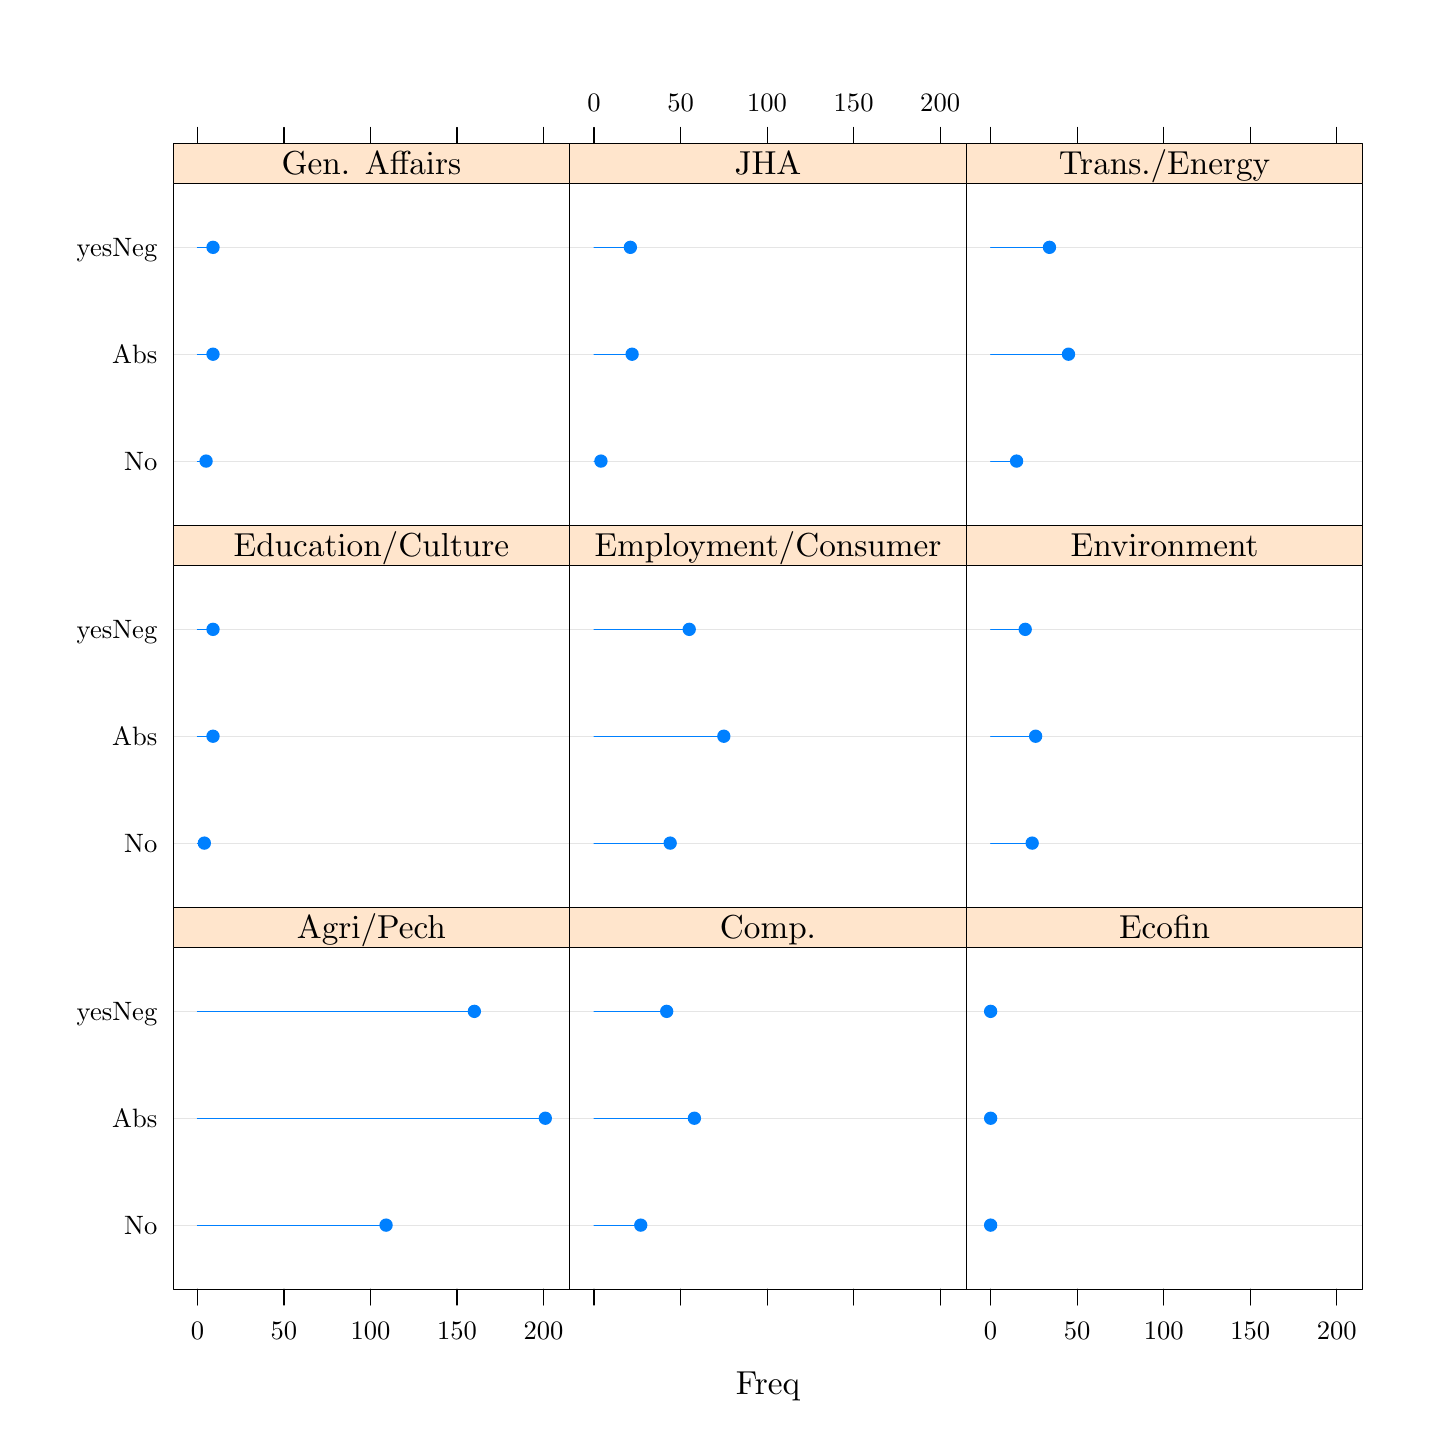
\begin{tikzpicture}[x=1pt,y=1pt]
\definecolor[named]{drawColor}{rgb}{0.00,0.00,0.00}
\definecolor[named]{fillColor}{rgb}{1.00,1.00,1.00}
\fill[color=fillColor,] (0,0) rectangle (505.89,505.89);
\begin{scope}
\path[clip] (  0.00,  0.00) rectangle (505.89,505.89);
\end{scope}
\begin{scope}
\path[clip] (  0.00,  0.00) rectangle (505.89,505.89);

\draw[fill opacity=0.00,draw opacity=0.00,] (  0.00,  0.00) rectangle (505.89,505.89);
\definecolor[named]{drawColor}{rgb}{0.00,0.00,0.00}

\node[color=drawColor,anchor=base,inner sep=0pt, outer sep=0pt, scale=  1.20] at (267.50, 12.04) {Freq%
};
\end{scope}
\begin{scope}
\path[clip] (  0.00,  0.00) rectangle (505.89,505.89);
\end{scope}
\begin{scope}
\path[clip] (  0.00,  0.00) rectangle (505.89,505.89);
\end{scope}
\begin{scope}
\path[clip] (  0.00,  0.00) rectangle (505.89,505.89);
\end{scope}
\begin{scope}
\path[clip] ( 52.54, 50.02) rectangle (195.85,173.60);
\end{scope}
\begin{scope}
\path[clip] (  0.00,  0.00) rectangle (505.89,505.89);
\end{scope}
\begin{scope}
\path[clip] (  0.00,  0.00) rectangle (505.89,505.89);
\end{scope}
\begin{scope}
\path[clip] (  0.00,  0.00) rectangle (505.89,505.89);
\end{scope}
\begin{scope}
\path[clip] (  0.00,  0.00) rectangle (505.89,505.89);
\definecolor[named]{drawColor}{rgb}{0.00,0.00,0.00}

\node[color=drawColor,anchor=base east,inner sep=0pt, outer sep=0pt, scale=  0.96] at ( 46.85, 69.88) {No%
};

\node[color=drawColor,anchor=base east,inner sep=0pt, outer sep=0pt, scale=  0.96] at ( 46.85,108.50) {Abs%
};

\node[color=drawColor,anchor=base east,inner sep=0pt, outer sep=0pt, scale=  0.96] at ( 46.85,147.12) {yesNeg%
};
\end{scope}
\begin{scope}
\path[clip] (  0.00,  0.00) rectangle (505.89,505.89);
\end{scope}
\begin{scope}
\path[clip] (  0.00,  0.00) rectangle (505.89,505.89);
\definecolor[named]{drawColor}{rgb}{0.00,0.00,0.00}

\draw[color=drawColor,line cap=round,line join=round,fill opacity=0.00,] ( 61.34, 50.02) -- ( 61.34, 44.32);

\draw[color=drawColor,line cap=round,line join=round,fill opacity=0.00,] ( 92.61, 50.02) -- ( 92.61, 44.32);

\draw[color=drawColor,line cap=round,line join=round,fill opacity=0.00,] (123.88, 50.02) -- (123.88, 44.32);

\draw[color=drawColor,line cap=round,line join=round,fill opacity=0.00,] (155.15, 50.02) -- (155.15, 44.32);

\draw[color=drawColor,line cap=round,line join=round,fill opacity=0.00,] (186.42, 50.02) -- (186.42, 44.32);

\node[color=drawColor,anchor=base,inner sep=0pt, outer sep=0pt, scale=  0.96] at ( 61.34, 32.02) {0%
};

\node[color=drawColor,anchor=base,inner sep=0pt, outer sep=0pt, scale=  0.96] at ( 92.61, 32.02) {50%
};

\node[color=drawColor,anchor=base,inner sep=0pt, outer sep=0pt, scale=  0.96] at (123.88, 32.02) {100%
};

\node[color=drawColor,anchor=base,inner sep=0pt, outer sep=0pt, scale=  0.96] at (155.15, 32.02) {150%
};

\node[color=drawColor,anchor=base,inner sep=0pt, outer sep=0pt, scale=  0.96] at (186.42, 32.02) {200%
};
\end{scope}
\begin{scope}
\path[clip] (  0.00,  0.00) rectangle (505.89,505.89);
\end{scope}
\begin{scope}
\path[clip] ( 52.54, 50.02) rectangle (195.85,173.60);
\definecolor[named]{drawColor}{rgb}{0.90,0.90,0.90}

\draw[color=drawColor,line cap=round,line join=round,fill opacity=0.00,] ( 52.54, 73.19) -- (195.85, 73.19);

\draw[color=drawColor,line cap=round,line join=round,fill opacity=0.00,] ( 52.54,111.81) -- (195.85,111.81);

\draw[color=drawColor,line cap=round,line join=round,fill opacity=0.00,] ( 52.54,150.43) -- (195.85,150.43);
\definecolor[named]{fillColor}{rgb}{0.00,0.50,1.00}

\draw[fill=fillColor,draw opacity=0.00,] (129.51, 73.19) circle (  2.41);

\draw[fill=fillColor,draw opacity=0.00,] (187.05,111.81) circle (  2.41);

\draw[fill=fillColor,draw opacity=0.00,] (161.41,150.43) circle (  2.41);
\definecolor[named]{drawColor}{rgb}{0.00,0.50,1.00}

\draw[color=drawColor,line cap=round,line join=round,fill opacity=0.00,] (129.51, 73.19) -- ( 61.34, 73.19);

\draw[color=drawColor,line cap=round,line join=round,fill opacity=0.00,] (187.05,111.81) -- ( 61.34,111.81);

\draw[color=drawColor,line cap=round,line join=round,fill opacity=0.00,] (161.41,150.43) -- ( 61.34,150.43);
\end{scope}
\begin{scope}
\path[clip] (  0.00,  0.00) rectangle (505.89,505.89);
\end{scope}
\begin{scope}
\path[clip] (  0.00,  0.00) rectangle (505.89,505.89);
\definecolor[named]{drawColor}{rgb}{0.00,0.00,0.00}

\draw[color=drawColor,line cap=round,line join=round,fill opacity=0.00,] ( 52.54, 50.02) rectangle (195.85,173.60);
\end{scope}
\begin{scope}
\path[clip] (  0.00,  0.00) rectangle (505.89,505.89);
\end{scope}
\begin{scope}
\path[clip] (  0.00,  0.00) rectangle (505.89,505.89);
\end{scope}
\begin{scope}
\path[clip] ( 52.54,173.60) rectangle (195.85,188.06);
\definecolor[named]{drawColor}{rgb}{1.00,0.90,0.80}
\definecolor[named]{fillColor}{rgb}{1.00,0.90,0.80}

\draw[color=drawColor,line cap=round,line join=round,fill=fillColor,] ( 52.54,173.60) rectangle (195.85,188.06);
\definecolor[named]{drawColor}{rgb}{0.00,0.00,0.00}

\node[color=drawColor,anchor=base west,inner sep=0pt, outer sep=0pt, scale=  1.20] at ( 97.27,176.70) {Agri/Pech%
};
\end{scope}
\begin{scope}
\path[clip] (  0.00,  0.00) rectangle (505.89,505.89);
\end{scope}
\begin{scope}
\path[clip] (  0.00,  0.00) rectangle (505.89,505.89);
\definecolor[named]{drawColor}{rgb}{0.00,0.00,0.00}

\draw[color=drawColor,line cap=round,line join=round,fill opacity=0.00,] ( 52.54,173.60) rectangle (195.85,188.06);
\end{scope}
\begin{scope}
\path[clip] (  0.00,  0.00) rectangle (505.89,505.89);
\end{scope}
\begin{scope}
\path[clip] (  0.00,  0.00) rectangle (505.89,505.89);
\end{scope}
\begin{scope}
\path[clip] (195.85, 50.02) rectangle (339.16,173.60);
\end{scope}
\begin{scope}
\path[clip] (  0.00,  0.00) rectangle (505.89,505.89);
\end{scope}
\begin{scope}
\path[clip] (  0.00,  0.00) rectangle (505.89,505.89);
\end{scope}
\begin{scope}
\path[clip] (  0.00,  0.00) rectangle (505.89,505.89);
\end{scope}
\begin{scope}
\path[clip] (  0.00,  0.00) rectangle (505.89,505.89);
\end{scope}
\begin{scope}
\path[clip] (  0.00,  0.00) rectangle (505.89,505.89);
\end{scope}
\begin{scope}
\path[clip] (  0.00,  0.00) rectangle (505.89,505.89);
\definecolor[named]{drawColor}{rgb}{0.00,0.00,0.00}

\draw[color=drawColor,line cap=round,line join=round,fill opacity=0.00,] (204.65, 50.02) -- (204.65, 44.32);

\draw[color=drawColor,line cap=round,line join=round,fill opacity=0.00,] (235.92, 50.02) -- (235.92, 44.32);

\draw[color=drawColor,line cap=round,line join=round,fill opacity=0.00,] (267.19, 50.02) -- (267.19, 44.32);

\draw[color=drawColor,line cap=round,line join=round,fill opacity=0.00,] (298.46, 50.02) -- (298.46, 44.32);

\draw[color=drawColor,line cap=round,line join=round,fill opacity=0.00,] (329.73, 50.02) -- (329.73, 44.32);
\end{scope}
\begin{scope}
\path[clip] (  0.00,  0.00) rectangle (505.89,505.89);
\end{scope}
\begin{scope}
\path[clip] (195.85, 50.02) rectangle (339.16,173.60);
\definecolor[named]{drawColor}{rgb}{0.90,0.90,0.90}

\draw[color=drawColor,line cap=round,line join=round,fill opacity=0.00,] (195.85, 73.19) -- (339.16, 73.19);

\draw[color=drawColor,line cap=round,line join=round,fill opacity=0.00,] (195.85,111.81) -- (339.16,111.81);

\draw[color=drawColor,line cap=round,line join=round,fill opacity=0.00,] (195.85,150.43) -- (339.16,150.43);
\definecolor[named]{fillColor}{rgb}{0.00,0.50,1.00}

\draw[fill=fillColor,draw opacity=0.00,] (221.53, 73.19) circle (  2.41);

\draw[fill=fillColor,draw opacity=0.00,] (240.92,111.81) circle (  2.41);

\draw[fill=fillColor,draw opacity=0.00,] (230.91,150.43) circle (  2.41);
\definecolor[named]{drawColor}{rgb}{0.00,0.50,1.00}

\draw[color=drawColor,line cap=round,line join=round,fill opacity=0.00,] (221.53, 73.19) -- (204.65, 73.19);

\draw[color=drawColor,line cap=round,line join=round,fill opacity=0.00,] (240.92,111.81) -- (204.65,111.81);

\draw[color=drawColor,line cap=round,line join=round,fill opacity=0.00,] (230.91,150.43) -- (204.65,150.43);
\end{scope}
\begin{scope}
\path[clip] (  0.00,  0.00) rectangle (505.89,505.89);
\end{scope}
\begin{scope}
\path[clip] (  0.00,  0.00) rectangle (505.89,505.89);
\definecolor[named]{drawColor}{rgb}{0.00,0.00,0.00}

\draw[color=drawColor,line cap=round,line join=round,fill opacity=0.00,] (195.85, 50.02) rectangle (339.16,173.60);
\end{scope}
\begin{scope}
\path[clip] (  0.00,  0.00) rectangle (505.89,505.89);
\end{scope}
\begin{scope}
\path[clip] (  0.00,  0.00) rectangle (505.89,505.89);
\end{scope}
\begin{scope}
\path[clip] (195.85,173.60) rectangle (339.16,188.06);
\definecolor[named]{drawColor}{rgb}{1.00,0.90,0.80}
\definecolor[named]{fillColor}{rgb}{1.00,0.90,0.80}

\draw[color=drawColor,line cap=round,line join=round,fill=fillColor,] (195.85,173.60) rectangle (339.16,188.06);
\definecolor[named]{drawColor}{rgb}{0.00,0.00,0.00}

\node[color=drawColor,anchor=base west,inner sep=0pt, outer sep=0pt, scale=  1.20] at (250.17,176.70) {Comp.%
};
\end{scope}
\begin{scope}
\path[clip] (  0.00,  0.00) rectangle (505.89,505.89);
\end{scope}
\begin{scope}
\path[clip] (  0.00,  0.00) rectangle (505.89,505.89);
\definecolor[named]{drawColor}{rgb}{0.00,0.00,0.00}

\draw[color=drawColor,line cap=round,line join=round,fill opacity=0.00,] (195.85,173.60) rectangle (339.16,188.06);
\end{scope}
\begin{scope}
\path[clip] (  0.00,  0.00) rectangle (505.89,505.89);
\end{scope}
\begin{scope}
\path[clip] (  0.00,  0.00) rectangle (505.89,505.89);
\end{scope}
\begin{scope}
\path[clip] (339.16, 50.02) rectangle (482.46,173.60);
\end{scope}
\begin{scope}
\path[clip] (  0.00,  0.00) rectangle (505.89,505.89);
\end{scope}
\begin{scope}
\path[clip] (  0.00,  0.00) rectangle (505.89,505.89);
\end{scope}
\begin{scope}
\path[clip] (  0.00,  0.00) rectangle (505.89,505.89);
\end{scope}
\begin{scope}
\path[clip] (  0.00,  0.00) rectangle (505.89,505.89);
\end{scope}
\begin{scope}
\path[clip] (  0.00,  0.00) rectangle (505.89,505.89);
\end{scope}
\begin{scope}
\path[clip] (  0.00,  0.00) rectangle (505.89,505.89);
\definecolor[named]{drawColor}{rgb}{0.00,0.00,0.00}

\draw[color=drawColor,line cap=round,line join=round,fill opacity=0.00,] (347.96, 50.02) -- (347.96, 44.32);

\draw[color=drawColor,line cap=round,line join=round,fill opacity=0.00,] (379.23, 50.02) -- (379.23, 44.32);

\draw[color=drawColor,line cap=round,line join=round,fill opacity=0.00,] (410.50, 50.02) -- (410.50, 44.32);

\draw[color=drawColor,line cap=round,line join=round,fill opacity=0.00,] (441.77, 50.02) -- (441.77, 44.32);

\draw[color=drawColor,line cap=round,line join=round,fill opacity=0.00,] (473.04, 50.02) -- (473.04, 44.32);

\node[color=drawColor,anchor=base,inner sep=0pt, outer sep=0pt, scale=  0.96] at (347.96, 32.02) {0%
};

\node[color=drawColor,anchor=base,inner sep=0pt, outer sep=0pt, scale=  0.96] at (379.23, 32.02) {50%
};

\node[color=drawColor,anchor=base,inner sep=0pt, outer sep=0pt, scale=  0.96] at (410.50, 32.02) {100%
};

\node[color=drawColor,anchor=base,inner sep=0pt, outer sep=0pt, scale=  0.96] at (441.77, 32.02) {150%
};

\node[color=drawColor,anchor=base,inner sep=0pt, outer sep=0pt, scale=  0.96] at (473.04, 32.02) {200%
};
\end{scope}
\begin{scope}
\path[clip] (  0.00,  0.00) rectangle (505.89,505.89);
\end{scope}
\begin{scope}
\path[clip] (339.16, 50.02) rectangle (482.46,173.60);
\definecolor[named]{drawColor}{rgb}{0.90,0.90,0.90}

\draw[color=drawColor,line cap=round,line join=round,fill opacity=0.00,] (339.16, 73.19) -- (482.46, 73.19);

\draw[color=drawColor,line cap=round,line join=round,fill opacity=0.00,] (339.16,111.81) -- (482.46,111.81);

\draw[color=drawColor,line cap=round,line join=round,fill opacity=0.00,] (339.16,150.43) -- (482.46,150.43);
\definecolor[named]{fillColor}{rgb}{0.00,0.50,1.00}

\draw[fill=fillColor,draw opacity=0.00,] (347.96, 73.19) circle (  2.41);

\draw[fill=fillColor,draw opacity=0.00,] (347.96,111.81) circle (  2.41);

\draw[fill=fillColor,draw opacity=0.00,] (347.96,150.43) circle (  2.41);
\definecolor[named]{drawColor}{rgb}{0.00,0.50,1.00}

\draw[color=drawColor,line cap=round,line join=round,fill opacity=0.00,] (347.96, 73.19) -- (347.96, 73.19);

\draw[color=drawColor,line cap=round,line join=round,fill opacity=0.00,] (347.96,111.81) -- (347.96,111.81);

\draw[color=drawColor,line cap=round,line join=round,fill opacity=0.00,] (347.96,150.43) -- (347.96,150.43);
\end{scope}
\begin{scope}
\path[clip] (  0.00,  0.00) rectangle (505.89,505.89);
\end{scope}
\begin{scope}
\path[clip] (  0.00,  0.00) rectangle (505.89,505.89);
\definecolor[named]{drawColor}{rgb}{0.00,0.00,0.00}

\draw[color=drawColor,line cap=round,line join=round,fill opacity=0.00,] (339.16, 50.02) rectangle (482.46,173.60);
\end{scope}
\begin{scope}
\path[clip] (  0.00,  0.00) rectangle (505.89,505.89);
\end{scope}
\begin{scope}
\path[clip] (  0.00,  0.00) rectangle (505.89,505.89);
\end{scope}
\begin{scope}
\path[clip] (339.16,173.60) rectangle (482.46,188.06);
\definecolor[named]{drawColor}{rgb}{1.00,0.90,0.80}
\definecolor[named]{fillColor}{rgb}{1.00,0.90,0.80}

\draw[color=drawColor,line cap=round,line join=round,fill=fillColor,] (339.16,173.60) rectangle (482.46,188.06);
\definecolor[named]{drawColor}{rgb}{0.00,0.00,0.00}

\node[color=drawColor,anchor=base west,inner sep=0pt, outer sep=0pt, scale=  1.20] at (394.40,176.70) {Ecofin%
};
\end{scope}
\begin{scope}
\path[clip] (  0.00,  0.00) rectangle (505.89,505.89);
\end{scope}
\begin{scope}
\path[clip] (  0.00,  0.00) rectangle (505.89,505.89);
\definecolor[named]{drawColor}{rgb}{0.00,0.00,0.00}

\draw[color=drawColor,line cap=round,line join=round,fill opacity=0.00,] (339.16,173.60) rectangle (482.46,188.06);
\end{scope}
\begin{scope}
\path[clip] (  0.00,  0.00) rectangle (505.89,505.89);
\end{scope}
\begin{scope}
\path[clip] (  0.00,  0.00) rectangle (505.89,505.89);
\end{scope}
\begin{scope}
\path[clip] ( 52.54,188.06) rectangle (195.85,311.64);
\end{scope}
\begin{scope}
\path[clip] (  0.00,  0.00) rectangle (505.89,505.89);
\end{scope}
\begin{scope}
\path[clip] (  0.00,  0.00) rectangle (505.89,505.89);
\end{scope}
\begin{scope}
\path[clip] (  0.00,  0.00) rectangle (505.89,505.89);
\end{scope}
\begin{scope}
\path[clip] (  0.00,  0.00) rectangle (505.89,505.89);
\definecolor[named]{drawColor}{rgb}{0.00,0.00,0.00}

\node[color=drawColor,anchor=base east,inner sep=0pt, outer sep=0pt, scale=  0.96] at ( 46.85,207.92) {No%
};

\node[color=drawColor,anchor=base east,inner sep=0pt, outer sep=0pt, scale=  0.96] at ( 46.85,246.54) {Abs%
};

\node[color=drawColor,anchor=base east,inner sep=0pt, outer sep=0pt, scale=  0.96] at ( 46.85,285.17) {yesNeg%
};
\end{scope}
\begin{scope}
\path[clip] (  0.00,  0.00) rectangle (505.89,505.89);
\end{scope}
\begin{scope}
\path[clip] (  0.00,  0.00) rectangle (505.89,505.89);
\end{scope}
\begin{scope}
\path[clip] (  0.00,  0.00) rectangle (505.89,505.89);
\end{scope}
\begin{scope}
\path[clip] ( 52.54,188.06) rectangle (195.85,311.64);
\definecolor[named]{drawColor}{rgb}{0.90,0.90,0.90}

\draw[color=drawColor,line cap=round,line join=round,fill opacity=0.00,] ( 52.54,211.23) -- (195.85,211.23);

\draw[color=drawColor,line cap=round,line join=round,fill opacity=0.00,] ( 52.54,249.85) -- (195.85,249.85);

\draw[color=drawColor,line cap=round,line join=round,fill opacity=0.00,] ( 52.54,288.47) -- (195.85,288.47);
\definecolor[named]{fillColor}{rgb}{0.00,0.50,1.00}

\draw[fill=fillColor,draw opacity=0.00,] ( 63.84,211.23) circle (  2.41);

\draw[fill=fillColor,draw opacity=0.00,] ( 66.97,249.85) circle (  2.41);

\draw[fill=fillColor,draw opacity=0.00,] ( 66.97,288.47) circle (  2.41);
\definecolor[named]{drawColor}{rgb}{0.00,0.50,1.00}

\draw[color=drawColor,line cap=round,line join=round,fill opacity=0.00,] ( 63.84,211.23) -- ( 61.34,211.23);

\draw[color=drawColor,line cap=round,line join=round,fill opacity=0.00,] ( 66.97,249.85) -- ( 61.34,249.85);

\draw[color=drawColor,line cap=round,line join=round,fill opacity=0.00,] ( 66.97,288.47) -- ( 61.34,288.47);
\end{scope}
\begin{scope}
\path[clip] (  0.00,  0.00) rectangle (505.89,505.89);
\end{scope}
\begin{scope}
\path[clip] (  0.00,  0.00) rectangle (505.89,505.89);
\definecolor[named]{drawColor}{rgb}{0.00,0.00,0.00}

\draw[color=drawColor,line cap=round,line join=round,fill opacity=0.00,] ( 52.54,188.06) rectangle (195.85,311.64);
\end{scope}
\begin{scope}
\path[clip] (  0.00,  0.00) rectangle (505.89,505.89);
\end{scope}
\begin{scope}
\path[clip] (  0.00,  0.00) rectangle (505.89,505.89);
\end{scope}
\begin{scope}
\path[clip] ( 52.54,311.64) rectangle (195.85,326.10);
\definecolor[named]{drawColor}{rgb}{1.00,0.90,0.80}
\definecolor[named]{fillColor}{rgb}{1.00,0.90,0.80}

\draw[color=drawColor,line cap=round,line join=round,fill=fillColor,] ( 52.54,311.64) rectangle (195.85,326.10);
\definecolor[named]{drawColor}{rgb}{0.00,0.00,0.00}

\node[color=drawColor,anchor=base west,inner sep=0pt, outer sep=0pt, scale=  1.20] at ( 74.44,314.74) {Education/Culture%
};
\end{scope}
\begin{scope}
\path[clip] (  0.00,  0.00) rectangle (505.89,505.89);
\end{scope}
\begin{scope}
\path[clip] (  0.00,  0.00) rectangle (505.89,505.89);
\definecolor[named]{drawColor}{rgb}{0.00,0.00,0.00}

\draw[color=drawColor,line cap=round,line join=round,fill opacity=0.00,] ( 52.54,311.64) rectangle (195.85,326.10);
\end{scope}
\begin{scope}
\path[clip] (  0.00,  0.00) rectangle (505.89,505.89);
\end{scope}
\begin{scope}
\path[clip] (  0.00,  0.00) rectangle (505.89,505.89);
\end{scope}
\begin{scope}
\path[clip] (195.85,188.06) rectangle (339.16,311.64);
\end{scope}
\begin{scope}
\path[clip] (  0.00,  0.00) rectangle (505.89,505.89);
\end{scope}
\begin{scope}
\path[clip] (  0.00,  0.00) rectangle (505.89,505.89);
\end{scope}
\begin{scope}
\path[clip] (  0.00,  0.00) rectangle (505.89,505.89);
\end{scope}
\begin{scope}
\path[clip] (  0.00,  0.00) rectangle (505.89,505.89);
\end{scope}
\begin{scope}
\path[clip] (  0.00,  0.00) rectangle (505.89,505.89);
\end{scope}
\begin{scope}
\path[clip] (  0.00,  0.00) rectangle (505.89,505.89);
\end{scope}
\begin{scope}
\path[clip] (  0.00,  0.00) rectangle (505.89,505.89);
\end{scope}
\begin{scope}
\path[clip] (195.85,188.06) rectangle (339.16,311.64);
\definecolor[named]{drawColor}{rgb}{0.90,0.90,0.90}

\draw[color=drawColor,line cap=round,line join=round,fill opacity=0.00,] (195.85,211.23) -- (339.16,211.23);

\draw[color=drawColor,line cap=round,line join=round,fill opacity=0.00,] (195.85,249.85) -- (339.16,249.85);

\draw[color=drawColor,line cap=round,line join=round,fill opacity=0.00,] (195.85,288.47) -- (339.16,288.47);
\definecolor[named]{fillColor}{rgb}{0.00,0.50,1.00}

\draw[fill=fillColor,draw opacity=0.00,] (232.17,211.23) circle (  2.41);

\draw[fill=fillColor,draw opacity=0.00,] (251.55,249.85) circle (  2.41);

\draw[fill=fillColor,draw opacity=0.00,] (239.05,288.47) circle (  2.41);
\definecolor[named]{drawColor}{rgb}{0.00,0.50,1.00}

\draw[color=drawColor,line cap=round,line join=round,fill opacity=0.00,] (232.17,211.23) -- (204.65,211.23);

\draw[color=drawColor,line cap=round,line join=round,fill opacity=0.00,] (251.55,249.85) -- (204.65,249.85);

\draw[color=drawColor,line cap=round,line join=round,fill opacity=0.00,] (239.05,288.47) -- (204.65,288.47);
\end{scope}
\begin{scope}
\path[clip] (  0.00,  0.00) rectangle (505.89,505.89);
\end{scope}
\begin{scope}
\path[clip] (  0.00,  0.00) rectangle (505.89,505.89);
\definecolor[named]{drawColor}{rgb}{0.00,0.00,0.00}

\draw[color=drawColor,line cap=round,line join=round,fill opacity=0.00,] (195.85,188.06) rectangle (339.16,311.64);
\end{scope}
\begin{scope}
\path[clip] (  0.00,  0.00) rectangle (505.89,505.89);
\end{scope}
\begin{scope}
\path[clip] (  0.00,  0.00) rectangle (505.89,505.89);
\end{scope}
\begin{scope}
\path[clip] (195.85,311.64) rectangle (339.16,326.10);
\definecolor[named]{drawColor}{rgb}{1.00,0.90,0.80}
\definecolor[named]{fillColor}{rgb}{1.00,0.90,0.80}

\draw[color=drawColor,line cap=round,line join=round,fill=fillColor,] (195.85,311.64) rectangle (339.16,326.10);
\definecolor[named]{drawColor}{rgb}{0.00,0.00,0.00}

\node[color=drawColor,anchor=base west,inner sep=0pt, outer sep=0pt, scale=  1.20] at (204.88,314.74) {Employment/Consumer%
};
\end{scope}
\begin{scope}
\path[clip] (  0.00,  0.00) rectangle (505.89,505.89);
\end{scope}
\begin{scope}
\path[clip] (  0.00,  0.00) rectangle (505.89,505.89);
\definecolor[named]{drawColor}{rgb}{0.00,0.00,0.00}

\draw[color=drawColor,line cap=round,line join=round,fill opacity=0.00,] (195.85,311.64) rectangle (339.16,326.10);
\end{scope}
\begin{scope}
\path[clip] (  0.00,  0.00) rectangle (505.89,505.89);
\end{scope}
\begin{scope}
\path[clip] (  0.00,  0.00) rectangle (505.89,505.89);
\end{scope}
\begin{scope}
\path[clip] (339.16,188.06) rectangle (482.46,311.64);
\end{scope}
\begin{scope}
\path[clip] (  0.00,  0.00) rectangle (505.89,505.89);
\end{scope}
\begin{scope}
\path[clip] (  0.00,  0.00) rectangle (505.89,505.89);
\end{scope}
\begin{scope}
\path[clip] (  0.00,  0.00) rectangle (505.89,505.89);
\end{scope}
\begin{scope}
\path[clip] (  0.00,  0.00) rectangle (505.89,505.89);
\end{scope}
\begin{scope}
\path[clip] (  0.00,  0.00) rectangle (505.89,505.89);
\end{scope}
\begin{scope}
\path[clip] (  0.00,  0.00) rectangle (505.89,505.89);
\end{scope}
\begin{scope}
\path[clip] (  0.00,  0.00) rectangle (505.89,505.89);
\end{scope}
\begin{scope}
\path[clip] (339.16,188.06) rectangle (482.46,311.64);
\definecolor[named]{drawColor}{rgb}{0.90,0.90,0.90}

\draw[color=drawColor,line cap=round,line join=round,fill opacity=0.00,] (339.16,211.23) -- (482.46,211.23);

\draw[color=drawColor,line cap=round,line join=round,fill opacity=0.00,] (339.16,249.85) -- (482.46,249.85);

\draw[color=drawColor,line cap=round,line join=round,fill opacity=0.00,] (339.16,288.47) -- (482.46,288.47);
\definecolor[named]{fillColor}{rgb}{0.00,0.50,1.00}

\draw[fill=fillColor,draw opacity=0.00,] (362.97,211.23) circle (  2.41);

\draw[fill=fillColor,draw opacity=0.00,] (364.22,249.85) circle (  2.41);

\draw[fill=fillColor,draw opacity=0.00,] (360.46,288.47) circle (  2.41);
\definecolor[named]{drawColor}{rgb}{0.00,0.50,1.00}

\draw[color=drawColor,line cap=round,line join=round,fill opacity=0.00,] (362.97,211.23) -- (347.96,211.23);

\draw[color=drawColor,line cap=round,line join=round,fill opacity=0.00,] (364.22,249.85) -- (347.96,249.85);

\draw[color=drawColor,line cap=round,line join=round,fill opacity=0.00,] (360.46,288.47) -- (347.96,288.47);
\end{scope}
\begin{scope}
\path[clip] (  0.00,  0.00) rectangle (505.89,505.89);
\end{scope}
\begin{scope}
\path[clip] (  0.00,  0.00) rectangle (505.89,505.89);
\definecolor[named]{drawColor}{rgb}{0.00,0.00,0.00}

\draw[color=drawColor,line cap=round,line join=round,fill opacity=0.00,] (339.16,188.06) rectangle (482.46,311.64);
\end{scope}
\begin{scope}
\path[clip] (  0.00,  0.00) rectangle (505.89,505.89);
\end{scope}
\begin{scope}
\path[clip] (  0.00,  0.00) rectangle (505.89,505.89);
\end{scope}
\begin{scope}
\path[clip] (339.16,311.64) rectangle (482.46,326.10);
\definecolor[named]{drawColor}{rgb}{1.00,0.90,0.80}
\definecolor[named]{fillColor}{rgb}{1.00,0.90,0.80}

\draw[color=drawColor,line cap=round,line join=round,fill=fillColor,] (339.16,311.64) rectangle (482.46,326.10);
\definecolor[named]{drawColor}{rgb}{0.00,0.00,0.00}

\node[color=drawColor,anchor=base west,inner sep=0pt, outer sep=0pt, scale=  1.20] at (376.88,314.74) {Environment%
};
\end{scope}
\begin{scope}
\path[clip] (  0.00,  0.00) rectangle (505.89,505.89);
\end{scope}
\begin{scope}
\path[clip] (  0.00,  0.00) rectangle (505.89,505.89);
\definecolor[named]{drawColor}{rgb}{0.00,0.00,0.00}

\draw[color=drawColor,line cap=round,line join=round,fill opacity=0.00,] (339.16,311.64) rectangle (482.46,326.10);
\end{scope}
\begin{scope}
\path[clip] (  0.00,  0.00) rectangle (505.89,505.89);
\end{scope}
\begin{scope}
\path[clip] (  0.00,  0.00) rectangle (505.89,505.89);
\end{scope}
\begin{scope}
\path[clip] ( 52.54,326.10) rectangle (195.85,449.69);
\end{scope}
\begin{scope}
\path[clip] (  0.00,  0.00) rectangle (505.89,505.89);
\end{scope}
\begin{scope}
\path[clip] (  0.00,  0.00) rectangle (505.89,505.89);
\definecolor[named]{drawColor}{rgb}{0.00,0.00,0.00}

\draw[color=drawColor,line cap=round,line join=round,fill opacity=0.00,] ( 61.34,464.14) -- ( 61.34,469.83);

\draw[color=drawColor,line cap=round,line join=round,fill opacity=0.00,] ( 92.61,464.14) -- ( 92.61,469.83);

\draw[color=drawColor,line cap=round,line join=round,fill opacity=0.00,] (123.88,464.14) -- (123.88,469.83);

\draw[color=drawColor,line cap=round,line join=round,fill opacity=0.00,] (155.15,464.14) -- (155.15,469.83);

\draw[color=drawColor,line cap=round,line join=round,fill opacity=0.00,] (186.42,464.14) -- (186.42,469.83);
\end{scope}
\begin{scope}
\path[clip] (  0.00,  0.00) rectangle (505.89,505.89);
\end{scope}
\begin{scope}
\path[clip] (  0.00,  0.00) rectangle (505.89,505.89);
\definecolor[named]{drawColor}{rgb}{0.00,0.00,0.00}

\node[color=drawColor,anchor=base east,inner sep=0pt, outer sep=0pt, scale=  0.96] at ( 46.85,345.96) {No%
};

\node[color=drawColor,anchor=base east,inner sep=0pt, outer sep=0pt, scale=  0.96] at ( 46.85,384.59) {Abs%
};

\node[color=drawColor,anchor=base east,inner sep=0pt, outer sep=0pt, scale=  0.96] at ( 46.85,423.21) {yesNeg%
};
\end{scope}
\begin{scope}
\path[clip] (  0.00,  0.00) rectangle (505.89,505.89);
\end{scope}
\begin{scope}
\path[clip] (  0.00,  0.00) rectangle (505.89,505.89);
\end{scope}
\begin{scope}
\path[clip] (  0.00,  0.00) rectangle (505.89,505.89);
\end{scope}
\begin{scope}
\path[clip] ( 52.54,326.10) rectangle (195.85,449.69);
\definecolor[named]{drawColor}{rgb}{0.90,0.90,0.90}

\draw[color=drawColor,line cap=round,line join=round,fill opacity=0.00,] ( 52.54,349.27) -- (195.85,349.27);

\draw[color=drawColor,line cap=round,line join=round,fill opacity=0.00,] ( 52.54,387.89) -- (195.85,387.89);

\draw[color=drawColor,line cap=round,line join=round,fill opacity=0.00,] ( 52.54,426.51) -- (195.85,426.51);
\definecolor[named]{fillColor}{rgb}{0.00,0.50,1.00}

\draw[fill=fillColor,draw opacity=0.00,] ( 64.47,349.27) circle (  2.41);

\draw[fill=fillColor,draw opacity=0.00,] ( 66.97,387.89) circle (  2.41);

\draw[fill=fillColor,draw opacity=0.00,] ( 66.97,426.51) circle (  2.41);
\definecolor[named]{drawColor}{rgb}{0.00,0.50,1.00}

\draw[color=drawColor,line cap=round,line join=round,fill opacity=0.00,] ( 64.47,349.27) -- ( 61.34,349.27);

\draw[color=drawColor,line cap=round,line join=round,fill opacity=0.00,] ( 66.97,387.89) -- ( 61.34,387.89);

\draw[color=drawColor,line cap=round,line join=round,fill opacity=0.00,] ( 66.97,426.51) -- ( 61.34,426.51);
\end{scope}
\begin{scope}
\path[clip] (  0.00,  0.00) rectangle (505.89,505.89);
\end{scope}
\begin{scope}
\path[clip] (  0.00,  0.00) rectangle (505.89,505.89);
\definecolor[named]{drawColor}{rgb}{0.00,0.00,0.00}

\draw[color=drawColor,line cap=round,line join=round,fill opacity=0.00,] ( 52.54,326.10) rectangle (195.85,449.69);
\end{scope}
\begin{scope}
\path[clip] (  0.00,  0.00) rectangle (505.89,505.89);
\end{scope}
\begin{scope}
\path[clip] (  0.00,  0.00) rectangle (505.89,505.89);
\end{scope}
\begin{scope}
\path[clip] ( 52.54,449.69) rectangle (195.85,464.14);
\definecolor[named]{drawColor}{rgb}{1.00,0.90,0.80}
\definecolor[named]{fillColor}{rgb}{1.00,0.90,0.80}

\draw[color=drawColor,line cap=round,line join=round,fill=fillColor,] ( 52.54,449.69) rectangle (195.85,464.14);
\definecolor[named]{drawColor}{rgb}{0.00,0.00,0.00}

\node[color=drawColor,anchor=base west,inner sep=0pt, outer sep=0pt, scale=  1.20] at ( 91.78,452.78) {Gen. Affairs%
};
\end{scope}
\begin{scope}
\path[clip] (  0.00,  0.00) rectangle (505.89,505.89);
\end{scope}
\begin{scope}
\path[clip] (  0.00,  0.00) rectangle (505.89,505.89);
\definecolor[named]{drawColor}{rgb}{0.00,0.00,0.00}

\draw[color=drawColor,line cap=round,line join=round,fill opacity=0.00,] ( 52.54,449.69) rectangle (195.85,464.14);
\end{scope}
\begin{scope}
\path[clip] (  0.00,  0.00) rectangle (505.89,505.89);
\end{scope}
\begin{scope}
\path[clip] (  0.00,  0.00) rectangle (505.89,505.89);
\end{scope}
\begin{scope}
\path[clip] (195.85,326.10) rectangle (339.16,449.69);
\end{scope}
\begin{scope}
\path[clip] (  0.00,  0.00) rectangle (505.89,505.89);
\end{scope}
\begin{scope}
\path[clip] (  0.00,  0.00) rectangle (505.89,505.89);
\definecolor[named]{drawColor}{rgb}{0.00,0.00,0.00}

\draw[color=drawColor,line cap=round,line join=round,fill opacity=0.00,] (204.65,464.14) -- (204.65,469.83);

\draw[color=drawColor,line cap=round,line join=round,fill opacity=0.00,] (235.92,464.14) -- (235.92,469.83);

\draw[color=drawColor,line cap=round,line join=round,fill opacity=0.00,] (267.19,464.14) -- (267.19,469.83);

\draw[color=drawColor,line cap=round,line join=round,fill opacity=0.00,] (298.46,464.14) -- (298.46,469.83);

\draw[color=drawColor,line cap=round,line join=round,fill opacity=0.00,] (329.73,464.14) -- (329.73,469.83);

\node[color=drawColor,anchor=base,inner sep=0pt, outer sep=0pt, scale=  0.96] at (204.65,475.52) {0%
};

\node[color=drawColor,anchor=base,inner sep=0pt, outer sep=0pt, scale=  0.96] at (235.92,475.52) {50%
};

\node[color=drawColor,anchor=base,inner sep=0pt, outer sep=0pt, scale=  0.96] at (267.19,475.52) {100%
};

\node[color=drawColor,anchor=base,inner sep=0pt, outer sep=0pt, scale=  0.96] at (298.46,475.52) {150%
};

\node[color=drawColor,anchor=base,inner sep=0pt, outer sep=0pt, scale=  0.96] at (329.73,475.52) {200%
};
\end{scope}
\begin{scope}
\path[clip] (  0.00,  0.00) rectangle (505.89,505.89);
\end{scope}
\begin{scope}
\path[clip] (  0.00,  0.00) rectangle (505.89,505.89);
\end{scope}
\begin{scope}
\path[clip] (  0.00,  0.00) rectangle (505.89,505.89);
\end{scope}
\begin{scope}
\path[clip] (  0.00,  0.00) rectangle (505.89,505.89);
\end{scope}
\begin{scope}
\path[clip] (  0.00,  0.00) rectangle (505.89,505.89);
\end{scope}
\begin{scope}
\path[clip] (195.85,326.10) rectangle (339.16,449.69);
\definecolor[named]{drawColor}{rgb}{0.90,0.90,0.90}

\draw[color=drawColor,line cap=round,line join=round,fill opacity=0.00,] (195.85,349.27) -- (339.16,349.27);

\draw[color=drawColor,line cap=round,line join=round,fill opacity=0.00,] (195.85,387.89) -- (339.16,387.89);

\draw[color=drawColor,line cap=round,line join=round,fill opacity=0.00,] (195.85,426.51) -- (339.16,426.51);
\definecolor[named]{fillColor}{rgb}{0.00,0.50,1.00}

\draw[fill=fillColor,draw opacity=0.00,] (207.15,349.27) circle (  2.41);

\draw[fill=fillColor,draw opacity=0.00,] (218.41,387.89) circle (  2.41);

\draw[fill=fillColor,draw opacity=0.00,] (217.78,426.51) circle (  2.41);
\definecolor[named]{drawColor}{rgb}{0.00,0.50,1.00}

\draw[color=drawColor,line cap=round,line join=round,fill opacity=0.00,] (207.15,349.27) -- (204.65,349.27);

\draw[color=drawColor,line cap=round,line join=round,fill opacity=0.00,] (218.41,387.89) -- (204.65,387.89);

\draw[color=drawColor,line cap=round,line join=round,fill opacity=0.00,] (217.78,426.51) -- (204.65,426.51);
\end{scope}
\begin{scope}
\path[clip] (  0.00,  0.00) rectangle (505.89,505.89);
\end{scope}
\begin{scope}
\path[clip] (  0.00,  0.00) rectangle (505.89,505.89);
\definecolor[named]{drawColor}{rgb}{0.00,0.00,0.00}

\draw[color=drawColor,line cap=round,line join=round,fill opacity=0.00,] (195.85,326.10) rectangle (339.16,449.69);
\end{scope}
\begin{scope}
\path[clip] (  0.00,  0.00) rectangle (505.89,505.89);
\end{scope}
\begin{scope}
\path[clip] (  0.00,  0.00) rectangle (505.89,505.89);
\end{scope}
\begin{scope}
\path[clip] (195.85,449.69) rectangle (339.16,464.14);
\definecolor[named]{drawColor}{rgb}{1.00,0.90,0.80}
\definecolor[named]{fillColor}{rgb}{1.00,0.90,0.80}

\draw[color=drawColor,line cap=round,line join=round,fill=fillColor,] (195.85,449.69) rectangle (339.16,464.14);
\definecolor[named]{drawColor}{rgb}{0.00,0.00,0.00}

\node[color=drawColor,anchor=base west,inner sep=0pt, outer sep=0pt, scale=  1.20] at (255.42,452.78) {JHA%
};
\end{scope}
\begin{scope}
\path[clip] (  0.00,  0.00) rectangle (505.89,505.89);
\end{scope}
\begin{scope}
\path[clip] (  0.00,  0.00) rectangle (505.89,505.89);
\definecolor[named]{drawColor}{rgb}{0.00,0.00,0.00}

\draw[color=drawColor,line cap=round,line join=round,fill opacity=0.00,] (195.85,449.69) rectangle (339.16,464.14);
\end{scope}
\begin{scope}
\path[clip] (  0.00,  0.00) rectangle (505.89,505.89);
\end{scope}
\begin{scope}
\path[clip] (  0.00,  0.00) rectangle (505.89,505.89);
\end{scope}
\begin{scope}
\path[clip] (339.16,326.10) rectangle (482.46,449.69);
\end{scope}
\begin{scope}
\path[clip] (  0.00,  0.00) rectangle (505.89,505.89);
\end{scope}
\begin{scope}
\path[clip] (  0.00,  0.00) rectangle (505.89,505.89);
\definecolor[named]{drawColor}{rgb}{0.00,0.00,0.00}

\draw[color=drawColor,line cap=round,line join=round,fill opacity=0.00,] (347.96,464.14) -- (347.96,469.83);

\draw[color=drawColor,line cap=round,line join=round,fill opacity=0.00,] (379.23,464.14) -- (379.23,469.83);

\draw[color=drawColor,line cap=round,line join=round,fill opacity=0.00,] (410.50,464.14) -- (410.50,469.83);

\draw[color=drawColor,line cap=round,line join=round,fill opacity=0.00,] (441.77,464.14) -- (441.77,469.83);

\draw[color=drawColor,line cap=round,line join=round,fill opacity=0.00,] (473.04,464.14) -- (473.04,469.83);
\end{scope}
\begin{scope}
\path[clip] (  0.00,  0.00) rectangle (505.89,505.89);
\end{scope}
\begin{scope}
\path[clip] (  0.00,  0.00) rectangle (505.89,505.89);
\end{scope}
\begin{scope}
\path[clip] (  0.00,  0.00) rectangle (505.89,505.89);
\end{scope}
\begin{scope}
\path[clip] (  0.00,  0.00) rectangle (505.89,505.89);
\end{scope}
\begin{scope}
\path[clip] (  0.00,  0.00) rectangle (505.89,505.89);
\end{scope}
\begin{scope}
\path[clip] (339.16,326.10) rectangle (482.46,449.69);
\definecolor[named]{drawColor}{rgb}{0.90,0.90,0.90}

\draw[color=drawColor,line cap=round,line join=round,fill opacity=0.00,] (339.16,349.27) -- (482.46,349.27);

\draw[color=drawColor,line cap=round,line join=round,fill opacity=0.00,] (339.16,387.89) -- (482.46,387.89);

\draw[color=drawColor,line cap=round,line join=round,fill opacity=0.00,] (339.16,426.51) -- (482.46,426.51);
\definecolor[named]{fillColor}{rgb}{0.00,0.50,1.00}

\draw[fill=fillColor,draw opacity=0.00,] (357.34,349.27) circle (  2.41);

\draw[fill=fillColor,draw opacity=0.00,] (376.10,387.89) circle (  2.41);

\draw[fill=fillColor,draw opacity=0.00,] (369.22,426.51) circle (  2.41);
\definecolor[named]{drawColor}{rgb}{0.00,0.50,1.00}

\draw[color=drawColor,line cap=round,line join=round,fill opacity=0.00,] (357.34,349.27) -- (347.96,349.27);

\draw[color=drawColor,line cap=round,line join=round,fill opacity=0.00,] (376.10,387.89) -- (347.96,387.89);

\draw[color=drawColor,line cap=round,line join=round,fill opacity=0.00,] (369.22,426.51) -- (347.96,426.51);
\end{scope}
\begin{scope}
\path[clip] (  0.00,  0.00) rectangle (505.89,505.89);
\end{scope}
\begin{scope}
\path[clip] (  0.00,  0.00) rectangle (505.89,505.89);
\definecolor[named]{drawColor}{rgb}{0.00,0.00,0.00}

\draw[color=drawColor,line cap=round,line join=round,fill opacity=0.00,] (339.16,326.10) rectangle (482.46,449.69);
\end{scope}
\begin{scope}
\path[clip] (  0.00,  0.00) rectangle (505.89,505.89);
\end{scope}
\begin{scope}
\path[clip] (  0.00,  0.00) rectangle (505.89,505.89);
\end{scope}
\begin{scope}
\path[clip] (339.16,449.69) rectangle (482.46,464.14);
\definecolor[named]{drawColor}{rgb}{1.00,0.90,0.80}
\definecolor[named]{fillColor}{rgb}{1.00,0.90,0.80}

\draw[color=drawColor,line cap=round,line join=round,fill=fillColor,] (339.16,449.69) rectangle (482.46,464.14);
\definecolor[named]{drawColor}{rgb}{0.00,0.00,0.00}

\node[color=drawColor,anchor=base west,inner sep=0pt, outer sep=0pt, scale=  1.20] at (372.67,452.78) {Trans./Energy%
};
\end{scope}
\begin{scope}
\path[clip] (  0.00,  0.00) rectangle (505.89,505.89);
\end{scope}
\begin{scope}
\path[clip] (  0.00,  0.00) rectangle (505.89,505.89);
\definecolor[named]{drawColor}{rgb}{0.00,0.00,0.00}

\draw[color=drawColor,line cap=round,line join=round,fill opacity=0.00,] (339.16,449.69) rectangle (482.46,464.14);
\end{scope}
\begin{scope}
\path[clip] (  0.00,  0.00) rectangle (505.89,505.89);
\end{scope}
\begin{scope}
\path[clip] (  0.00,  0.00) rectangle (505.89,505.89);
\end{scope}
\begin{scope}
\path[clip] (  0.00,  0.00) rectangle (505.89,505.89);
\end{scope}
\begin{scope}
\path[clip] (  0.00,  0.00) rectangle (505.89,505.89);
\end{scope}
\end{tikzpicture}
}
\caption{}
\label{fig:depvar}
\end{figure}

In order to gauge the possible effect of the posited explanatory variables it is useful to tabulate them against the dependent variable. In figure \ref{fig:scatter} the squared government distance to the mean government left-right position in the Council has been plotted against the number of abstentions, no votes and yes votes with dissenting statements for each government. The plot is conditioned on whether a government is from an old or new member states, and for each category a regression line has been overlaid. 

\begin{figure}[htp]
\centering
\scalebox{.6}{\subfloat[][]{% Created by tikzDevice version 0.6.1 on 2011-07-25 15:12:06
% !TEX encoding = UTF-8 Unicode
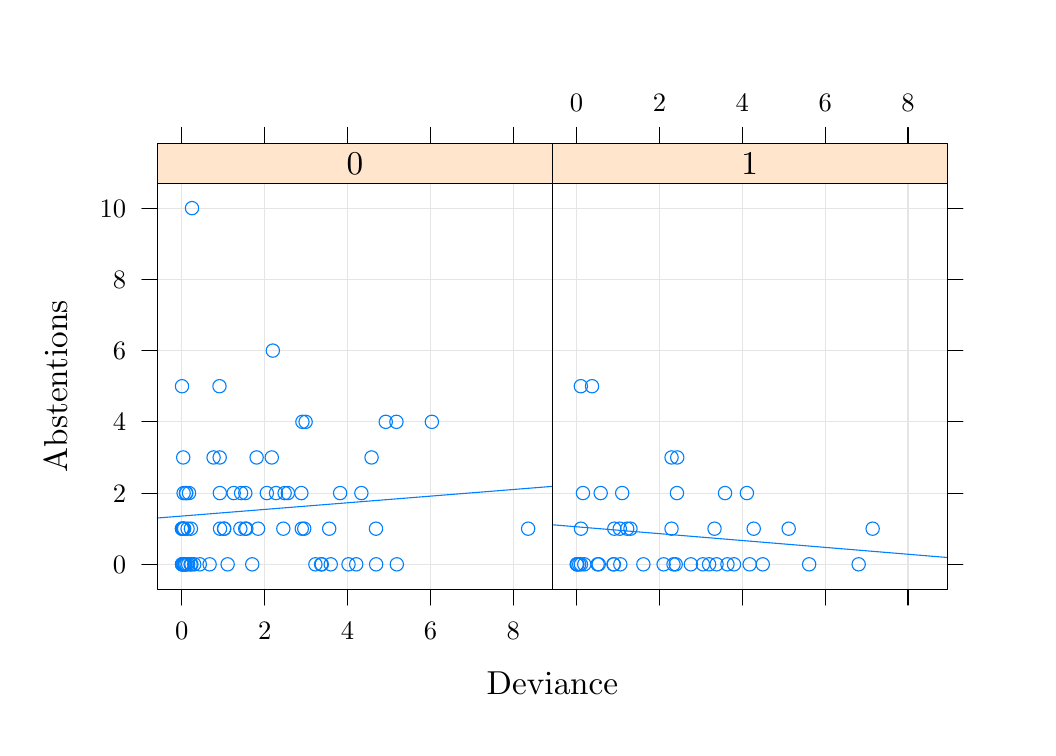
\begin{tikzpicture}[x=1pt,y=1pt]
\definecolor[named]{drawColor}{rgb}{0.00,0.00,0.00}
\definecolor[named]{fillColor}{rgb}{1.00,1.00,1.00}
\fill[color=fillColor,] (0,0) rectangle (361.35,252.94);
\begin{scope}
\path[clip] (  0.00,  0.00) rectangle (361.35,252.94);
\end{scope}
\begin{scope}
\path[clip] (  0.00,  0.00) rectangle (361.35,252.94);

\draw[fill opacity=0.00,draw opacity=0.00,] (  0.00,  0.00) rectangle (361.35,252.94);
\definecolor[named]{drawColor}{rgb}{0.00,0.00,0.00}

\node[color=drawColor,anchor=base,inner sep=0pt, outer sep=0pt, scale=  1.20] at (189.61, 12.04) {Deviance%
};
\end{scope}
\begin{scope}
\path[clip] (  0.00,  0.00) rectangle (361.35,252.94);
\definecolor[named]{drawColor}{rgb}{0.00,0.00,0.00}

\node[rotate= 90.00,color=drawColor,anchor=base,inner sep=0pt, outer sep=0pt, scale=  1.20] at ( 14.29,123.38) {Abstentions%
};
\end{scope}
\begin{scope}
\path[clip] (  0.00,  0.00) rectangle (361.35,252.94);
\end{scope}
\begin{scope}
\path[clip] (  0.00,  0.00) rectangle (361.35,252.94);
\end{scope}
\begin{scope}
\path[clip] (  0.00,  0.00) rectangle (361.35,252.94);
\end{scope}
\begin{scope}
\path[clip] ( 46.98, 50.02) rectangle (189.61,196.74);
\end{scope}
\begin{scope}
\path[clip] (  0.00,  0.00) rectangle (361.35,252.94);
\end{scope}
\begin{scope}
\path[clip] (  0.00,  0.00) rectangle (361.35,252.94);
\definecolor[named]{drawColor}{rgb}{0.00,0.00,0.00}

\draw[color=drawColor,line cap=round,line join=round,fill opacity=0.00,] ( 55.71,211.19) -- ( 55.71,216.88);

\draw[color=drawColor,line cap=round,line join=round,fill opacity=0.00,] ( 85.66,211.19) -- ( 85.66,216.88);

\draw[color=drawColor,line cap=round,line join=round,fill opacity=0.00,] (115.60,211.19) -- (115.60,216.88);

\draw[color=drawColor,line cap=round,line join=round,fill opacity=0.00,] (145.54,211.19) -- (145.54,216.88);

\draw[color=drawColor,line cap=round,line join=round,fill opacity=0.00,] (175.48,211.19) -- (175.48,216.88);
\end{scope}
\begin{scope}
\path[clip] (  0.00,  0.00) rectangle (361.35,252.94);
\end{scope}
\begin{scope}
\path[clip] (  0.00,  0.00) rectangle (361.35,252.94);
\definecolor[named]{drawColor}{rgb}{0.00,0.00,0.00}

\draw[color=drawColor,line cap=round,line join=round,fill opacity=0.00,] ( 46.98, 59.02) -- ( 41.29, 59.02);

\draw[color=drawColor,line cap=round,line join=round,fill opacity=0.00,] ( 46.98, 84.77) -- ( 41.29, 84.77);

\draw[color=drawColor,line cap=round,line join=round,fill opacity=0.00,] ( 46.98,110.51) -- ( 41.29,110.51);

\draw[color=drawColor,line cap=round,line join=round,fill opacity=0.00,] ( 46.98,136.25) -- ( 41.29,136.25);

\draw[color=drawColor,line cap=round,line join=round,fill opacity=0.00,] ( 46.98,161.99) -- ( 41.29,161.99);

\draw[color=drawColor,line cap=round,line join=round,fill opacity=0.00,] ( 46.98,187.73) -- ( 41.29,187.73);

\node[color=drawColor,anchor=base east,inner sep=0pt, outer sep=0pt, scale=  0.96] at ( 35.60, 55.72) {0%
};

\node[color=drawColor,anchor=base east,inner sep=0pt, outer sep=0pt, scale=  0.96] at ( 35.60, 81.46) {2%
};

\node[color=drawColor,anchor=base east,inner sep=0pt, outer sep=0pt, scale=  0.96] at ( 35.60,107.20) {4%
};

\node[color=drawColor,anchor=base east,inner sep=0pt, outer sep=0pt, scale=  0.96] at ( 35.60,132.94) {6%
};

\node[color=drawColor,anchor=base east,inner sep=0pt, outer sep=0pt, scale=  0.96] at ( 35.60,158.68) {8%
};

\node[color=drawColor,anchor=base east,inner sep=0pt, outer sep=0pt, scale=  0.96] at ( 35.60,184.42) {10%
};
\end{scope}
\begin{scope}
\path[clip] (  0.00,  0.00) rectangle (361.35,252.94);
\end{scope}
\begin{scope}
\path[clip] (  0.00,  0.00) rectangle (361.35,252.94);
\definecolor[named]{drawColor}{rgb}{0.00,0.00,0.00}

\draw[color=drawColor,line cap=round,line join=round,fill opacity=0.00,] ( 55.71, 50.02) -- ( 55.71, 44.32);

\draw[color=drawColor,line cap=round,line join=round,fill opacity=0.00,] ( 85.66, 50.02) -- ( 85.66, 44.32);

\draw[color=drawColor,line cap=round,line join=round,fill opacity=0.00,] (115.60, 50.02) -- (115.60, 44.32);

\draw[color=drawColor,line cap=round,line join=round,fill opacity=0.00,] (145.54, 50.02) -- (145.54, 44.32);

\draw[color=drawColor,line cap=round,line join=round,fill opacity=0.00,] (175.48, 50.02) -- (175.48, 44.32);

\node[color=drawColor,anchor=base,inner sep=0pt, outer sep=0pt, scale=  0.96] at ( 55.71, 32.02) {0%
};

\node[color=drawColor,anchor=base,inner sep=0pt, outer sep=0pt, scale=  0.96] at ( 85.66, 32.02) {2%
};

\node[color=drawColor,anchor=base,inner sep=0pt, outer sep=0pt, scale=  0.96] at (115.60, 32.02) {4%
};

\node[color=drawColor,anchor=base,inner sep=0pt, outer sep=0pt, scale=  0.96] at (145.54, 32.02) {6%
};

\node[color=drawColor,anchor=base,inner sep=0pt, outer sep=0pt, scale=  0.96] at (175.48, 32.02) {8%
};
\end{scope}
\begin{scope}
\path[clip] (  0.00,  0.00) rectangle (361.35,252.94);
\end{scope}
\begin{scope}
\path[clip] ( 46.98, 50.02) rectangle (189.61,196.74);
\definecolor[named]{drawColor}{rgb}{0.90,0.90,0.90}

\draw[color=drawColor,line cap=round,line join=round,fill opacity=0.00,] ( 46.98, 59.02) -- (189.61, 59.02);

\draw[color=drawColor,line cap=round,line join=round,fill opacity=0.00,] ( 46.98, 84.77) -- (189.61, 84.77);

\draw[color=drawColor,line cap=round,line join=round,fill opacity=0.00,] ( 46.98,110.51) -- (189.61,110.51);

\draw[color=drawColor,line cap=round,line join=round,fill opacity=0.00,] ( 46.98,136.25) -- (189.61,136.25);

\draw[color=drawColor,line cap=round,line join=round,fill opacity=0.00,] ( 46.98,161.99) -- (189.61,161.99);

\draw[color=drawColor,line cap=round,line join=round,fill opacity=0.00,] ( 46.98,187.73) -- (189.61,187.73);

\draw[color=drawColor,line cap=round,line join=round,fill opacity=0.00,] ( 55.71, 50.02) -- ( 55.71,196.74);

\draw[color=drawColor,line cap=round,line join=round,fill opacity=0.00,] ( 85.66, 50.02) -- ( 85.66,196.74);

\draw[color=drawColor,line cap=round,line join=round,fill opacity=0.00,] (115.60, 50.02) -- (115.60,196.74);

\draw[color=drawColor,line cap=round,line join=round,fill opacity=0.00,] (145.54, 50.02) -- (145.54,196.74);

\draw[color=drawColor,line cap=round,line join=round,fill opacity=0.00,] (175.48, 50.02) -- (175.48,196.74);
\definecolor[named]{drawColor}{rgb}{0.00,0.50,1.00}

\draw[color=drawColor,line cap=round,line join=round,fill opacity=0.00,] ( 58.00, 59.02) circle (  2.41);

\draw[color=drawColor,line cap=round,line join=round,fill opacity=0.00,] ( 58.30, 84.77) circle (  2.41);

\draw[color=drawColor,line cap=round,line join=round,fill opacity=0.00,] ( 59.17, 59.02) circle (  2.41);

\draw[color=drawColor,line cap=round,line join=round,fill opacity=0.00,] (125.86, 71.90) circle (  2.41);

\draw[color=drawColor,line cap=round,line join=round,fill opacity=0.00,] ( 60.19, 59.02) circle (  2.41);

\draw[color=drawColor,line cap=round,line join=round,fill opacity=0.00,] ( 92.38, 71.90) circle (  2.41);

\draw[color=drawColor,line cap=round,line join=round,fill opacity=0.00,] ( 70.94, 71.90) circle (  2.41);

\draw[color=drawColor,line cap=round,line join=round,fill opacity=0.00,] ( 55.79, 59.02) circle (  2.41);

\draw[color=drawColor,line cap=round,line join=round,fill opacity=0.00,] ( 56.21, 97.64) circle (  2.41);

\draw[color=drawColor,line cap=round,line join=round,fill opacity=0.00,] ( 56.64, 59.02) circle (  2.41);

\draw[color=drawColor,line cap=round,line join=round,fill opacity=0.00,] ( 69.31,123.38) circle (  2.41);

\draw[color=drawColor,line cap=round,line join=round,fill opacity=0.00,] ( 59.38,187.73) circle (  2.41);

\draw[color=drawColor,line cap=round,line join=round,fill opacity=0.00,] ( 56.81, 59.02) circle (  2.41);

\draw[color=drawColor,line cap=round,line join=round,fill opacity=0.00,] ( 57.40, 59.02) circle (  2.41);

\draw[color=drawColor,line cap=round,line join=round,fill opacity=0.00,] ( 89.74, 84.77) circle (  2.41);

\draw[color=drawColor,line cap=round,line join=round,fill opacity=0.00,] (106.27, 59.02) circle (  2.41);

\draw[color=drawColor,line cap=round,line join=round,fill opacity=0.00,] (103.97, 59.02) circle (  2.41);

\draw[color=drawColor,line cap=round,line join=round,fill opacity=0.00,] (106.03, 59.02) circle (  2.41);

\draw[color=drawColor,line cap=round,line join=round,fill opacity=0.00,] ( 56.94, 59.02) circle (  2.41);

\draw[color=drawColor,line cap=round,line join=round,fill opacity=0.00,] ( 62.20, 59.02) circle (  2.41);

\draw[color=drawColor,line cap=round,line join=round,fill opacity=0.00,] ( 55.86, 59.02) circle (  2.41);

\draw[color=drawColor,line cap=round,line join=round,fill opacity=0.00,] ( 56.54, 71.90) circle (  2.41);

\draw[color=drawColor,line cap=round,line join=round,fill opacity=0.00,] ( 69.51, 71.90) circle (  2.41);

\draw[color=drawColor,line cap=round,line join=round,fill opacity=0.00,] ( 57.77, 71.90) circle (  2.41);

\draw[color=drawColor,line cap=round,line join=round,fill opacity=0.00,] ( 57.32, 84.77) circle (  2.41);

\draw[color=drawColor,line cap=round,line join=round,fill opacity=0.00,] (115.94, 59.02) circle (  2.41);

\draw[color=drawColor,line cap=round,line join=round,fill opacity=0.00,] (120.58, 84.77) circle (  2.41);

\draw[color=drawColor,line cap=round,line join=round,fill opacity=0.00,] (129.39,110.51) circle (  2.41);

\draw[color=drawColor,line cap=round,line join=round,fill opacity=0.00,] ( 72.25, 59.02) circle (  2.41);

\draw[color=drawColor,line cap=round,line join=round,fill opacity=0.00,] ( 69.44, 84.77) circle (  2.41);

\draw[color=drawColor,line cap=round,line join=round,fill opacity=0.00,] ( 77.12, 84.77) circle (  2.41);

\draw[color=drawColor,line cap=round,line join=round,fill opacity=0.00,] ( 86.42, 84.77) circle (  2.41);

\draw[color=drawColor,line cap=round,line join=round,fill opacity=0.00,] ( 57.17, 84.77) circle (  2.41);

\draw[color=drawColor,line cap=round,line join=round,fill opacity=0.00,] (100.43,110.51) circle (  2.41);

\draw[color=drawColor,line cap=round,line join=round,fill opacity=0.00,] (146.05,110.51) circle (  2.41);

\draw[color=drawColor,line cap=round,line join=round,fill opacity=0.00,] ( 69.38, 97.64) circle (  2.41);

\draw[color=drawColor,line cap=round,line join=round,fill opacity=0.00,] ( 71.04, 71.90) circle (  2.41);

\draw[color=drawColor,line cap=round,line join=round,fill opacity=0.00,] ( 56.33, 59.02) circle (  2.41);

\draw[color=drawColor,line cap=round,line join=round,fill opacity=0.00,] ( 74.44, 84.77) circle (  2.41);

\draw[color=drawColor,line cap=round,line join=round,fill opacity=0.00,] (125.92, 59.02) circle (  2.41);

\draw[color=drawColor,line cap=round,line join=round,fill opacity=0.00,] ( 83.26, 71.90) circle (  2.41);

\draw[color=drawColor,line cap=round,line join=round,fill opacity=0.00,] ( 55.78, 71.90) circle (  2.41);

\draw[color=drawColor,line cap=round,line join=round,fill opacity=0.00,] ( 55.74, 71.90) circle (  2.41);

\draw[color=drawColor,line cap=round,line join=round,fill opacity=0.00,] (124.26, 97.64) circle (  2.41);

\draw[color=drawColor,line cap=round,line join=round,fill opacity=0.00,] ( 88.58,136.25) circle (  2.41);

\draw[color=drawColor,line cap=round,line join=round,fill opacity=0.00,] ( 99.94, 71.90) circle (  2.41);

\draw[color=drawColor,line cap=round,line join=round,fill opacity=0.00,] (108.96, 71.90) circle (  2.41);

\draw[color=drawColor,line cap=round,line join=round,fill opacity=0.00,] (109.51, 59.02) circle (  2.41);

\draw[color=drawColor,line cap=round,line join=round,fill opacity=0.00,] (118.72, 59.02) circle (  2.41);

\draw[color=drawColor,line cap=round,line join=round,fill opacity=0.00,] (133.39, 59.02) circle (  2.41);

\draw[color=drawColor,line cap=round,line join=round,fill opacity=0.00,] ( 65.74, 59.02) circle (  2.41);

\draw[color=drawColor,line cap=round,line join=round,fill opacity=0.00,] ( 92.85, 84.77) circle (  2.41);

\draw[color=drawColor,line cap=round,line join=round,fill opacity=0.00,] ( 55.77,123.38) circle (  2.41);

\draw[color=drawColor,line cap=round,line join=round,fill opacity=0.00,] ( 55.80, 59.02) circle (  2.41);

\draw[color=drawColor,line cap=round,line join=round,fill opacity=0.00,] ( 81.15, 59.02) circle (  2.41);

\draw[color=drawColor,line cap=round,line join=round,fill opacity=0.00,] ( 56.28, 59.02) circle (  2.41);

\draw[color=drawColor,line cap=round,line join=round,fill opacity=0.00,] ( 56.35, 84.77) circle (  2.41);

\draw[color=drawColor,line cap=round,line join=round,fill opacity=0.00,] ( 56.32, 71.90) circle (  2.41);

\draw[color=drawColor,line cap=round,line join=round,fill opacity=0.00,] ( 56.06, 71.90) circle (  2.41);

\draw[color=drawColor,line cap=round,line join=round,fill opacity=0.00,] ( 78.61, 71.90) circle (  2.41);

\draw[color=drawColor,line cap=round,line join=round,fill opacity=0.00,] ( 58.87, 59.02) circle (  2.41);

\draw[color=drawColor,line cap=round,line join=round,fill opacity=0.00,] ( 67.17, 97.64) circle (  2.41);

\draw[color=drawColor,line cap=round,line join=round,fill opacity=0.00,] ( 99.05, 71.90) circle (  2.41);

\draw[color=drawColor,line cap=round,line join=round,fill opacity=0.00,] ( 82.73, 97.64) circle (  2.41);

\draw[color=drawColor,line cap=round,line join=round,fill opacity=0.00,] (180.85, 71.90) circle (  2.41);

\draw[color=drawColor,line cap=round,line join=round,fill opacity=0.00,] (112.90, 84.77) circle (  2.41);

\draw[color=drawColor,line cap=round,line join=round,fill opacity=0.00,] ( 99.28,110.51) circle (  2.41);

\draw[color=drawColor,line cap=round,line join=round,fill opacity=0.00,] ( 98.89, 84.77) circle (  2.41);

\draw[color=drawColor,line cap=round,line join=round,fill opacity=0.00,] ( 94.02, 84.77) circle (  2.41);

\draw[color=drawColor,line cap=round,line join=round,fill opacity=0.00,] (133.25,110.51) circle (  2.41);

\draw[color=drawColor,line cap=round,line join=round,fill opacity=0.00,] ( 79.01, 71.90) circle (  2.41);

\draw[color=drawColor,line cap=round,line join=round,fill opacity=0.00,] ( 58.98, 71.90) circle (  2.41);

\draw[color=drawColor,line cap=round,line join=round,fill opacity=0.00,] ( 88.20, 97.64) circle (  2.41);

\draw[color=drawColor,line cap=round,line join=round,fill opacity=0.00,] ( 76.85, 71.90) circle (  2.41);

\draw[color=drawColor,line cap=round,line join=round,fill opacity=0.00,] ( 78.64, 84.77) circle (  2.41);

\draw[color=drawColor,line cap=round,line join=round,fill opacity=0.00,] (189.61, 87.19) --
	( 46.98, 75.76);
\end{scope}
\begin{scope}
\path[clip] (  0.00,  0.00) rectangle (361.35,252.94);
\end{scope}
\begin{scope}
\path[clip] (  0.00,  0.00) rectangle (361.35,252.94);
\definecolor[named]{drawColor}{rgb}{0.00,0.00,0.00}

\draw[color=drawColor,line cap=round,line join=round,fill opacity=0.00,] ( 46.98, 50.02) rectangle (189.61,196.74);
\end{scope}
\begin{scope}
\path[clip] (  0.00,  0.00) rectangle (361.35,252.94);
\end{scope}
\begin{scope}
\path[clip] (  0.00,  0.00) rectangle (361.35,252.94);
\end{scope}
\begin{scope}
\path[clip] ( 46.98,196.74) rectangle (189.61,211.19);
\definecolor[named]{drawColor}{rgb}{1.00,0.90,0.80}
\definecolor[named]{fillColor}{rgb}{1.00,0.90,0.80}

\draw[color=drawColor,line cap=round,line join=round,fill=fillColor,] ( 46.98,196.74) rectangle (189.61,211.19);
\definecolor[named]{drawColor}{rgb}{0.00,0.00,0.00}

\node[color=drawColor,anchor=base west,inner sep=0pt, outer sep=0pt, scale=  1.20] at (115.29,199.83) {0%
};
\end{scope}
\begin{scope}
\path[clip] (  0.00,  0.00) rectangle (361.35,252.94);
\end{scope}
\begin{scope}
\path[clip] (  0.00,  0.00) rectangle (361.35,252.94);
\definecolor[named]{drawColor}{rgb}{0.00,0.00,0.00}

\draw[color=drawColor,line cap=round,line join=round,fill opacity=0.00,] ( 46.98,196.74) rectangle (189.61,211.19);
\end{scope}
\begin{scope}
\path[clip] (  0.00,  0.00) rectangle (361.35,252.94);
\end{scope}
\begin{scope}
\path[clip] (  0.00,  0.00) rectangle (361.35,252.94);
\end{scope}
\begin{scope}
\path[clip] (189.61, 50.02) rectangle (332.23,196.74);
\end{scope}
\begin{scope}
\path[clip] (  0.00,  0.00) rectangle (361.35,252.94);
\end{scope}
\begin{scope}
\path[clip] (  0.00,  0.00) rectangle (361.35,252.94);
\definecolor[named]{drawColor}{rgb}{0.00,0.00,0.00}

\draw[color=drawColor,line cap=round,line join=round,fill opacity=0.00,] (198.34,211.19) -- (198.34,216.88);

\draw[color=drawColor,line cap=round,line join=round,fill opacity=0.00,] (228.28,211.19) -- (228.28,216.88);

\draw[color=drawColor,line cap=round,line join=round,fill opacity=0.00,] (258.23,211.19) -- (258.23,216.88);

\draw[color=drawColor,line cap=round,line join=round,fill opacity=0.00,] (288.17,211.19) -- (288.17,216.88);

\draw[color=drawColor,line cap=round,line join=round,fill opacity=0.00,] (318.11,211.19) -- (318.11,216.88);

\node[color=drawColor,anchor=base,inner sep=0pt, outer sep=0pt, scale=  0.96] at (198.34,222.58) {0%
};

\node[color=drawColor,anchor=base,inner sep=0pt, outer sep=0pt, scale=  0.96] at (228.28,222.58) {2%
};

\node[color=drawColor,anchor=base,inner sep=0pt, outer sep=0pt, scale=  0.96] at (258.23,222.58) {4%
};

\node[color=drawColor,anchor=base,inner sep=0pt, outer sep=0pt, scale=  0.96] at (288.17,222.58) {6%
};

\node[color=drawColor,anchor=base,inner sep=0pt, outer sep=0pt, scale=  0.96] at (318.11,222.58) {8%
};
\end{scope}
\begin{scope}
\path[clip] (  0.00,  0.00) rectangle (361.35,252.94);
\end{scope}
\begin{scope}
\path[clip] (  0.00,  0.00) rectangle (361.35,252.94);
\end{scope}
\begin{scope}
\path[clip] (  0.00,  0.00) rectangle (361.35,252.94);
\end{scope}
\begin{scope}
\path[clip] (  0.00,  0.00) rectangle (361.35,252.94);
\definecolor[named]{drawColor}{rgb}{0.00,0.00,0.00}

\draw[color=drawColor,line cap=round,line join=round,fill opacity=0.00,] (198.34, 50.02) -- (198.34, 44.32);

\draw[color=drawColor,line cap=round,line join=round,fill opacity=0.00,] (228.28, 50.02) -- (228.28, 44.32);

\draw[color=drawColor,line cap=round,line join=round,fill opacity=0.00,] (258.23, 50.02) -- (258.23, 44.32);

\draw[color=drawColor,line cap=round,line join=round,fill opacity=0.00,] (288.17, 50.02) -- (288.17, 44.32);

\draw[color=drawColor,line cap=round,line join=round,fill opacity=0.00,] (318.11, 50.02) -- (318.11, 44.32);

\draw[color=drawColor,line cap=round,line join=round,fill opacity=0.00,] (332.23, 59.02) -- (337.92, 59.02);

\draw[color=drawColor,line cap=round,line join=round,fill opacity=0.00,] (332.23, 84.77) -- (337.92, 84.77);

\draw[color=drawColor,line cap=round,line join=round,fill opacity=0.00,] (332.23,110.51) -- (337.92,110.51);

\draw[color=drawColor,line cap=round,line join=round,fill opacity=0.00,] (332.23,136.25) -- (337.92,136.25);

\draw[color=drawColor,line cap=round,line join=round,fill opacity=0.00,] (332.23,161.99) -- (337.92,161.99);

\draw[color=drawColor,line cap=round,line join=round,fill opacity=0.00,] (332.23,187.73) -- (337.92,187.73);
\end{scope}
\begin{scope}
\path[clip] (  0.00,  0.00) rectangle (361.35,252.94);
\end{scope}
\begin{scope}
\path[clip] (189.61, 50.02) rectangle (332.23,196.74);
\definecolor[named]{drawColor}{rgb}{0.90,0.90,0.90}

\draw[color=drawColor,line cap=round,line join=round,fill opacity=0.00,] (189.61, 59.02) -- (332.23, 59.02);

\draw[color=drawColor,line cap=round,line join=round,fill opacity=0.00,] (189.61, 84.77) -- (332.23, 84.77);

\draw[color=drawColor,line cap=round,line join=round,fill opacity=0.00,] (189.61,110.51) -- (332.23,110.51);

\draw[color=drawColor,line cap=round,line join=round,fill opacity=0.00,] (189.61,136.25) -- (332.23,136.25);

\draw[color=drawColor,line cap=round,line join=round,fill opacity=0.00,] (189.61,161.99) -- (332.23,161.99);

\draw[color=drawColor,line cap=round,line join=round,fill opacity=0.00,] (189.61,187.73) -- (332.23,187.73);

\draw[color=drawColor,line cap=round,line join=round,fill opacity=0.00,] (198.34, 50.02) -- (198.34,196.74);

\draw[color=drawColor,line cap=round,line join=round,fill opacity=0.00,] (228.28, 50.02) -- (228.28,196.74);

\draw[color=drawColor,line cap=round,line join=round,fill opacity=0.00,] (258.23, 50.02) -- (258.23,196.74);

\draw[color=drawColor,line cap=round,line join=round,fill opacity=0.00,] (288.17, 50.02) -- (288.17,196.74);

\draw[color=drawColor,line cap=round,line join=round,fill opacity=0.00,] (318.11, 50.02) -- (318.11,196.74);
\definecolor[named]{drawColor}{rgb}{0.00,0.50,1.00}

\draw[color=drawColor,line cap=round,line join=round,fill opacity=0.00,] (211.98, 71.90) circle (  2.41);

\draw[color=drawColor,line cap=round,line join=round,fill opacity=0.00,] (262.35, 71.90) circle (  2.41);

\draw[color=drawColor,line cap=round,line join=round,fill opacity=0.00,] (234.72, 97.64) circle (  2.41);

\draw[color=drawColor,line cap=round,line join=round,fill opacity=0.00,] (214.15, 59.02) circle (  2.41);

\draw[color=drawColor,line cap=round,line join=round,fill opacity=0.00,] (198.57, 59.02) circle (  2.41);

\draw[color=drawColor,line cap=round,line join=round,fill opacity=0.00,] (198.38, 59.02) circle (  2.41);

\draw[color=drawColor,line cap=round,line join=round,fill opacity=0.00,] (198.60, 59.02) circle (  2.41);

\draw[color=drawColor,line cap=round,line join=round,fill opacity=0.00,] (246.22, 59.02) circle (  2.41);

\draw[color=drawColor,line cap=round,line join=round,fill opacity=0.00,] (203.93,123.38) circle (  2.41);

\draw[color=drawColor,line cap=round,line join=round,fill opacity=0.00,] (199.93, 71.90) circle (  2.41);

\draw[color=drawColor,line cap=round,line join=round,fill opacity=0.00,] (214.83, 84.77) circle (  2.41);

\draw[color=drawColor,line cap=round,line join=round,fill opacity=0.00,] (274.99, 71.90) circle (  2.41);

\draw[color=drawColor,line cap=round,line join=round,fill opacity=0.00,] (217.82, 71.90) circle (  2.41);

\draw[color=drawColor,line cap=round,line join=round,fill opacity=0.00,] (300.27, 59.02) circle (  2.41);

\draw[color=drawColor,line cap=round,line join=round,fill opacity=0.00,] (259.89, 84.77) circle (  2.41);

\draw[color=drawColor,line cap=round,line join=round,fill opacity=0.00,] (305.32, 71.90) circle (  2.41);

\draw[color=drawColor,line cap=round,line join=round,fill opacity=0.00,] (252.86, 59.02) circle (  2.41);

\draw[color=drawColor,line cap=round,line join=round,fill opacity=0.00,] (255.23, 59.02) circle (  2.41);

\draw[color=drawColor,line cap=round,line join=round,fill opacity=0.00,] (234.62, 84.77) circle (  2.41);

\draw[color=drawColor,line cap=round,line join=round,fill opacity=0.00,] (211.67, 59.02) circle (  2.41);

\draw[color=drawColor,line cap=round,line join=round,fill opacity=0.00,] (233.37, 59.02) circle (  2.41);

\draw[color=drawColor,line cap=round,line join=round,fill opacity=0.00,] (216.63, 71.90) circle (  2.41);

\draw[color=drawColor,line cap=round,line join=round,fill opacity=0.00,] (211.81, 59.02) circle (  2.41);

\draw[color=drawColor,line cap=round,line join=round,fill opacity=0.00,] (232.66, 97.64) circle (  2.41);

\draw[color=drawColor,line cap=round,line join=round,fill opacity=0.00,] (234.16, 59.02) circle (  2.41);

\draw[color=drawColor,line cap=round,line join=round,fill opacity=0.00,] (232.65, 71.90) circle (  2.41);

\draw[color=drawColor,line cap=round,line join=round,fill opacity=0.00,] (239.63, 59.02) circle (  2.41);

\draw[color=drawColor,line cap=round,line join=round,fill opacity=0.00,] (199.88,123.38) circle (  2.41);

\draw[color=drawColor,line cap=round,line join=round,fill opacity=0.00,] (265.62, 59.02) circle (  2.41);

\draw[color=drawColor,line cap=round,line join=round,fill opacity=0.00,] (205.95, 59.02) circle (  2.41);

\draw[color=drawColor,line cap=round,line join=round,fill opacity=0.00,] (207.05, 84.77) circle (  2.41);

\draw[color=drawColor,line cap=round,line join=round,fill opacity=0.00,] (251.99, 84.77) circle (  2.41);

\draw[color=drawColor,line cap=round,line join=round,fill opacity=0.00,] (248.19, 71.90) circle (  2.41);

\draw[color=drawColor,line cap=round,line join=round,fill opacity=0.00,] (282.38, 59.02) circle (  2.41);

\draw[color=drawColor,line cap=round,line join=round,fill opacity=0.00,] (260.87, 59.02) circle (  2.41);

\draw[color=drawColor,line cap=round,line join=round,fill opacity=0.00,] (199.29, 59.02) circle (  2.41);

\draw[color=drawColor,line cap=round,line join=round,fill opacity=0.00,] (213.95, 71.90) circle (  2.41);

\draw[color=drawColor,line cap=round,line join=round,fill opacity=0.00,] (199.91, 59.02) circle (  2.41);

\draw[color=drawColor,line cap=round,line join=round,fill opacity=0.00,] (200.65, 84.77) circle (  2.41);

\draw[color=drawColor,line cap=round,line join=round,fill opacity=0.00,] (229.79, 59.02) circle (  2.41);

\draw[color=drawColor,line cap=round,line join=round,fill opacity=0.00,] (222.48, 59.02) circle (  2.41);

\draw[color=drawColor,line cap=round,line join=round,fill opacity=0.00,] (201.13, 59.02) circle (  2.41);

\draw[color=drawColor,line cap=round,line join=round,fill opacity=0.00,] (206.35, 59.02) circle (  2.41);

\draw[color=drawColor,line cap=round,line join=round,fill opacity=0.00,] (248.92, 59.02) circle (  2.41);

\draw[color=drawColor,line cap=round,line join=round,fill opacity=0.00,] (244.00, 59.02) circle (  2.41);

\draw[color=drawColor,line cap=round,line join=round,fill opacity=0.00,] (332.23, 61.49) --
	(189.61, 73.31);
\end{scope}
\begin{scope}
\path[clip] (  0.00,  0.00) rectangle (361.35,252.94);
\end{scope}
\begin{scope}
\path[clip] (  0.00,  0.00) rectangle (361.35,252.94);
\definecolor[named]{drawColor}{rgb}{0.00,0.00,0.00}

\draw[color=drawColor,line cap=round,line join=round,fill opacity=0.00,] (189.61, 50.02) rectangle (332.23,196.74);
\end{scope}
\begin{scope}
\path[clip] (  0.00,  0.00) rectangle (361.35,252.94);
\end{scope}
\begin{scope}
\path[clip] (  0.00,  0.00) rectangle (361.35,252.94);
\end{scope}
\begin{scope}
\path[clip] (189.61,196.74) rectangle (332.23,211.19);
\definecolor[named]{drawColor}{rgb}{1.00,0.90,0.80}
\definecolor[named]{fillColor}{rgb}{1.00,0.90,0.80}

\draw[color=drawColor,line cap=round,line join=round,fill=fillColor,] (189.61,196.74) rectangle (332.23,211.19);
\definecolor[named]{drawColor}{rgb}{0.00,0.00,0.00}

\node[color=drawColor,anchor=base west,inner sep=0pt, outer sep=0pt, scale=  1.20] at (257.92,199.83) {1%
};
\end{scope}
\begin{scope}
\path[clip] (  0.00,  0.00) rectangle (361.35,252.94);
\end{scope}
\begin{scope}
\path[clip] (  0.00,  0.00) rectangle (361.35,252.94);
\definecolor[named]{drawColor}{rgb}{0.00,0.00,0.00}

\draw[color=drawColor,line cap=round,line join=round,fill opacity=0.00,] (189.61,196.74) rectangle (332.23,211.19);
\end{scope}
\begin{scope}
\path[clip] (  0.00,  0.00) rectangle (361.35,252.94);
\end{scope}
\begin{scope}
\path[clip] (  0.00,  0.00) rectangle (361.35,252.94);
\end{scope}
\begin{scope}
\path[clip] (  0.00,  0.00) rectangle (361.35,252.94);
\end{scope}
\begin{scope}
\path[clip] (  0.00,  0.00) rectangle (361.35,252.94);
\end{scope}
\end{tikzpicture}
}}\quad
\scalebox{.6}{\subfloat[][]{% Created by tikzDevice version 0.6.1 on 2011-07-25 15:12:07
% !TEX encoding = UTF-8 Unicode
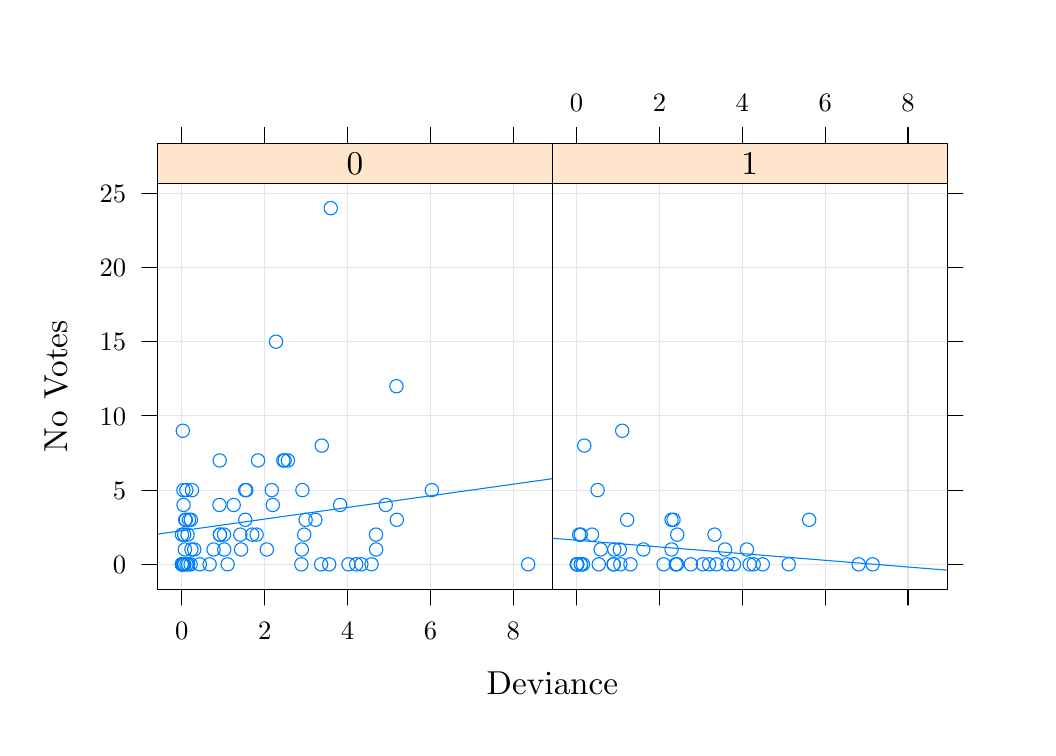
\begin{tikzpicture}[x=1pt,y=1pt]
\definecolor[named]{drawColor}{rgb}{0.00,0.00,0.00}
\definecolor[named]{fillColor}{rgb}{1.00,1.00,1.00}
\fill[color=fillColor,] (0,0) rectangle (361.35,252.94);
\begin{scope}
\path[clip] (  0.00,  0.00) rectangle (361.35,252.94);
\end{scope}
\begin{scope}
\path[clip] (  0.00,  0.00) rectangle (361.35,252.94);

\draw[fill opacity=0.00,draw opacity=0.00,] (  0.00,  0.00) rectangle (361.35,252.94);
\definecolor[named]{drawColor}{rgb}{0.00,0.00,0.00}

\node[color=drawColor,anchor=base,inner sep=0pt, outer sep=0pt, scale=  1.20] at (189.61, 12.04) {Deviance%
};
\end{scope}
\begin{scope}
\path[clip] (  0.00,  0.00) rectangle (361.35,252.94);
\definecolor[named]{drawColor}{rgb}{0.00,0.00,0.00}

\node[rotate= 90.00,color=drawColor,anchor=base,inner sep=0pt, outer sep=0pt, scale=  1.20] at ( 14.29,123.38) {No Votes%
};
\end{scope}
\begin{scope}
\path[clip] (  0.00,  0.00) rectangle (361.35,252.94);
\end{scope}
\begin{scope}
\path[clip] (  0.00,  0.00) rectangle (361.35,252.94);
\end{scope}
\begin{scope}
\path[clip] (  0.00,  0.00) rectangle (361.35,252.94);
\end{scope}
\begin{scope}
\path[clip] ( 46.98, 50.02) rectangle (189.61,196.74);
\end{scope}
\begin{scope}
\path[clip] (  0.00,  0.00) rectangle (361.35,252.94);
\end{scope}
\begin{scope}
\path[clip] (  0.00,  0.00) rectangle (361.35,252.94);
\definecolor[named]{drawColor}{rgb}{0.00,0.00,0.00}

\draw[color=drawColor,line cap=round,line join=round,fill opacity=0.00,] ( 55.71,211.19) -- ( 55.71,216.88);

\draw[color=drawColor,line cap=round,line join=round,fill opacity=0.00,] ( 85.66,211.19) -- ( 85.66,216.88);

\draw[color=drawColor,line cap=round,line join=round,fill opacity=0.00,] (115.60,211.19) -- (115.60,216.88);

\draw[color=drawColor,line cap=round,line join=round,fill opacity=0.00,] (145.54,211.19) -- (145.54,216.88);

\draw[color=drawColor,line cap=round,line join=round,fill opacity=0.00,] (175.48,211.19) -- (175.48,216.88);
\end{scope}
\begin{scope}
\path[clip] (  0.00,  0.00) rectangle (361.35,252.94);
\end{scope}
\begin{scope}
\path[clip] (  0.00,  0.00) rectangle (361.35,252.94);
\definecolor[named]{drawColor}{rgb}{0.00,0.00,0.00}

\draw[color=drawColor,line cap=round,line join=round,fill opacity=0.00,] ( 46.98, 59.02) -- ( 41.29, 59.02);

\draw[color=drawColor,line cap=round,line join=round,fill opacity=0.00,] ( 46.98, 85.84) -- ( 41.29, 85.84);

\draw[color=drawColor,line cap=round,line join=round,fill opacity=0.00,] ( 46.98,112.65) -- ( 41.29,112.65);

\draw[color=drawColor,line cap=round,line join=round,fill opacity=0.00,] ( 46.98,139.47) -- ( 41.29,139.47);

\draw[color=drawColor,line cap=round,line join=round,fill opacity=0.00,] ( 46.98,166.28) -- ( 41.29,166.28);

\draw[color=drawColor,line cap=round,line join=round,fill opacity=0.00,] ( 46.98,193.09) -- ( 41.29,193.09);

\node[color=drawColor,anchor=base east,inner sep=0pt, outer sep=0pt, scale=  0.96] at ( 35.60, 55.72) {0%
};

\node[color=drawColor,anchor=base east,inner sep=0pt, outer sep=0pt, scale=  0.96] at ( 35.60, 82.53) {5%
};

\node[color=drawColor,anchor=base east,inner sep=0pt, outer sep=0pt, scale=  0.96] at ( 35.60,109.35) {10%
};

\node[color=drawColor,anchor=base east,inner sep=0pt, outer sep=0pt, scale=  0.96] at ( 35.60,136.16) {15%
};

\node[color=drawColor,anchor=base east,inner sep=0pt, outer sep=0pt, scale=  0.96] at ( 35.60,162.97) {20%
};

\node[color=drawColor,anchor=base east,inner sep=0pt, outer sep=0pt, scale=  0.96] at ( 35.60,189.79) {25%
};
\end{scope}
\begin{scope}
\path[clip] (  0.00,  0.00) rectangle (361.35,252.94);
\end{scope}
\begin{scope}
\path[clip] (  0.00,  0.00) rectangle (361.35,252.94);
\definecolor[named]{drawColor}{rgb}{0.00,0.00,0.00}

\draw[color=drawColor,line cap=round,line join=round,fill opacity=0.00,] ( 55.71, 50.02) -- ( 55.71, 44.32);

\draw[color=drawColor,line cap=round,line join=round,fill opacity=0.00,] ( 85.66, 50.02) -- ( 85.66, 44.32);

\draw[color=drawColor,line cap=round,line join=round,fill opacity=0.00,] (115.60, 50.02) -- (115.60, 44.32);

\draw[color=drawColor,line cap=round,line join=round,fill opacity=0.00,] (145.54, 50.02) -- (145.54, 44.32);

\draw[color=drawColor,line cap=round,line join=round,fill opacity=0.00,] (175.48, 50.02) -- (175.48, 44.32);

\node[color=drawColor,anchor=base,inner sep=0pt, outer sep=0pt, scale=  0.96] at ( 55.71, 32.02) {0%
};

\node[color=drawColor,anchor=base,inner sep=0pt, outer sep=0pt, scale=  0.96] at ( 85.66, 32.02) {2%
};

\node[color=drawColor,anchor=base,inner sep=0pt, outer sep=0pt, scale=  0.96] at (115.60, 32.02) {4%
};

\node[color=drawColor,anchor=base,inner sep=0pt, outer sep=0pt, scale=  0.96] at (145.54, 32.02) {6%
};

\node[color=drawColor,anchor=base,inner sep=0pt, outer sep=0pt, scale=  0.96] at (175.48, 32.02) {8%
};
\end{scope}
\begin{scope}
\path[clip] (  0.00,  0.00) rectangle (361.35,252.94);
\end{scope}
\begin{scope}
\path[clip] ( 46.98, 50.02) rectangle (189.61,196.74);
\definecolor[named]{drawColor}{rgb}{0.90,0.90,0.90}

\draw[color=drawColor,line cap=round,line join=round,fill opacity=0.00,] ( 46.98, 59.02) -- (189.61, 59.02);

\draw[color=drawColor,line cap=round,line join=round,fill opacity=0.00,] ( 46.98, 85.84) -- (189.61, 85.84);

\draw[color=drawColor,line cap=round,line join=round,fill opacity=0.00,] ( 46.98,112.65) -- (189.61,112.65);

\draw[color=drawColor,line cap=round,line join=round,fill opacity=0.00,] ( 46.98,139.47) -- (189.61,139.47);

\draw[color=drawColor,line cap=round,line join=round,fill opacity=0.00,] ( 46.98,166.28) -- (189.61,166.28);

\draw[color=drawColor,line cap=round,line join=round,fill opacity=0.00,] ( 46.98,193.09) -- (189.61,193.09);

\draw[color=drawColor,line cap=round,line join=round,fill opacity=0.00,] ( 55.71, 50.02) -- ( 55.71,196.74);

\draw[color=drawColor,line cap=round,line join=round,fill opacity=0.00,] ( 85.66, 50.02) -- ( 85.66,196.74);

\draw[color=drawColor,line cap=round,line join=round,fill opacity=0.00,] (115.60, 50.02) -- (115.60,196.74);

\draw[color=drawColor,line cap=round,line join=round,fill opacity=0.00,] (145.54, 50.02) -- (145.54,196.74);

\draw[color=drawColor,line cap=round,line join=round,fill opacity=0.00,] (175.48, 50.02) -- (175.48,196.74);
\definecolor[named]{drawColor}{rgb}{0.00,0.50,1.00}

\draw[color=drawColor,line cap=round,line join=round,fill opacity=0.00,] ( 58.00, 59.02) circle (  2.41);

\draw[color=drawColor,line cap=round,line join=round,fill opacity=0.00,] ( 58.30, 75.11) circle (  2.41);

\draw[color=drawColor,line cap=round,line join=round,fill opacity=0.00,] ( 59.17, 64.39) circle (  2.41);

\draw[color=drawColor,line cap=round,line join=round,fill opacity=0.00,] (125.86, 69.75) circle (  2.41);

\draw[color=drawColor,line cap=round,line join=round,fill opacity=0.00,] ( 60.19, 64.39) circle (  2.41);

\draw[color=drawColor,line cap=round,line join=round,fill opacity=0.00,] ( 92.38, 96.56) circle (  2.41);

\draw[color=drawColor,line cap=round,line join=round,fill opacity=0.00,] ( 70.94, 69.75) circle (  2.41);

\draw[color=drawColor,line cap=round,line join=round,fill opacity=0.00,] ( 55.79, 59.02) circle (  2.41);

\draw[color=drawColor,line cap=round,line join=round,fill opacity=0.00,] ( 56.21, 59.02) circle (  2.41);

\draw[color=drawColor,line cap=round,line join=round,fill opacity=0.00,] ( 56.64, 59.02) circle (  2.41);

\draw[color=drawColor,line cap=round,line join=round,fill opacity=0.00,] ( 69.31, 80.48) circle (  2.41);

\draw[color=drawColor,line cap=round,line join=round,fill opacity=0.00,] ( 59.38, 85.84) circle (  2.41);

\draw[color=drawColor,line cap=round,line join=round,fill opacity=0.00,] ( 56.81, 64.39) circle (  2.41);

\draw[color=drawColor,line cap=round,line join=round,fill opacity=0.00,] ( 57.40, 59.02) circle (  2.41);

\draw[color=drawColor,line cap=round,line join=round,fill opacity=0.00,] ( 89.74,139.47) circle (  2.41);

\draw[color=drawColor,line cap=round,line join=round,fill opacity=0.00,] (106.27,101.93) circle (  2.41);

\draw[color=drawColor,line cap=round,line join=round,fill opacity=0.00,] (103.97, 75.11) circle (  2.41);

\draw[color=drawColor,line cap=round,line join=round,fill opacity=0.00,] (106.03, 59.02) circle (  2.41);

\draw[color=drawColor,line cap=round,line join=round,fill opacity=0.00,] ( 56.94, 75.11) circle (  2.41);

\draw[color=drawColor,line cap=round,line join=round,fill opacity=0.00,] ( 62.20, 59.02) circle (  2.41);

\draw[color=drawColor,line cap=round,line join=round,fill opacity=0.00,] ( 55.86, 59.02) circle (  2.41);

\draw[color=drawColor,line cap=round,line join=round,fill opacity=0.00,] ( 56.54, 69.75) circle (  2.41);

\draw[color=drawColor,line cap=round,line join=round,fill opacity=0.00,] ( 69.51, 69.75) circle (  2.41);

\draw[color=drawColor,line cap=round,line join=round,fill opacity=0.00,] ( 57.77, 69.75) circle (  2.41);

\draw[color=drawColor,line cap=round,line join=round,fill opacity=0.00,] ( 57.32, 85.84) circle (  2.41);

\draw[color=drawColor,line cap=round,line join=round,fill opacity=0.00,] (115.94, 59.02) circle (  2.41);

\draw[color=drawColor,line cap=round,line join=round,fill opacity=0.00,] (120.58, 59.02) circle (  2.41);

\draw[color=drawColor,line cap=round,line join=round,fill opacity=0.00,] (129.39, 80.48) circle (  2.41);

\draw[color=drawColor,line cap=round,line join=round,fill opacity=0.00,] ( 72.25, 59.02) circle (  2.41);

\draw[color=drawColor,line cap=round,line join=round,fill opacity=0.00,] ( 69.44, 69.75) circle (  2.41);

\draw[color=drawColor,line cap=round,line join=round,fill opacity=0.00,] ( 77.12, 64.39) circle (  2.41);

\draw[color=drawColor,line cap=round,line join=round,fill opacity=0.00,] ( 86.42, 64.39) circle (  2.41);

\draw[color=drawColor,line cap=round,line join=round,fill opacity=0.00,] ( 57.17, 75.11) circle (  2.41);

\draw[color=drawColor,line cap=round,line join=round,fill opacity=0.00,] (100.43, 75.11) circle (  2.41);

\draw[color=drawColor,line cap=round,line join=round,fill opacity=0.00,] (146.05, 85.84) circle (  2.41);

\draw[color=drawColor,line cap=round,line join=round,fill opacity=0.00,] ( 69.38, 96.56) circle (  2.41);

\draw[color=drawColor,line cap=round,line join=round,fill opacity=0.00,] ( 71.04, 64.39) circle (  2.41);

\draw[color=drawColor,line cap=round,line join=round,fill opacity=0.00,] ( 56.33, 59.02) circle (  2.41);

\draw[color=drawColor,line cap=round,line join=round,fill opacity=0.00,] ( 74.44, 80.48) circle (  2.41);

\draw[color=drawColor,line cap=round,line join=round,fill opacity=0.00,] (125.92, 64.39) circle (  2.41);

\draw[color=drawColor,line cap=round,line join=round,fill opacity=0.00,] ( 83.26, 96.56) circle (  2.41);

\draw[color=drawColor,line cap=round,line join=round,fill opacity=0.00,] ( 55.78, 59.02) circle (  2.41);

\draw[color=drawColor,line cap=round,line join=round,fill opacity=0.00,] ( 55.74, 59.02) circle (  2.41);

\draw[color=drawColor,line cap=round,line join=round,fill opacity=0.00,] (124.26, 59.02) circle (  2.41);

\draw[color=drawColor,line cap=round,line join=round,fill opacity=0.00,] ( 88.58, 80.48) circle (  2.41);

\draw[color=drawColor,line cap=round,line join=round,fill opacity=0.00,] ( 99.94, 69.75) circle (  2.41);

\draw[color=drawColor,line cap=round,line join=round,fill opacity=0.00,] (108.96, 59.02) circle (  2.41);

\draw[color=drawColor,line cap=round,line join=round,fill opacity=0.00,] (109.51,187.73) circle (  2.41);

\draw[color=drawColor,line cap=round,line join=round,fill opacity=0.00,] (118.72, 59.02) circle (  2.41);

\draw[color=drawColor,line cap=round,line join=round,fill opacity=0.00,] (133.39, 75.11) circle (  2.41);

\draw[color=drawColor,line cap=round,line join=round,fill opacity=0.00,] ( 65.74, 59.02) circle (  2.41);

\draw[color=drawColor,line cap=round,line join=round,fill opacity=0.00,] ( 92.85, 96.56) circle (  2.41);

\draw[color=drawColor,line cap=round,line join=round,fill opacity=0.00,] ( 55.77, 69.75) circle (  2.41);

\draw[color=drawColor,line cap=round,line join=round,fill opacity=0.00,] ( 55.80, 59.02) circle (  2.41);

\draw[color=drawColor,line cap=round,line join=round,fill opacity=0.00,] ( 81.15, 69.75) circle (  2.41);

\draw[color=drawColor,line cap=round,line join=round,fill opacity=0.00,] ( 56.28, 85.84) circle (  2.41);

\draw[color=drawColor,line cap=round,line join=round,fill opacity=0.00,] ( 56.35, 59.02) circle (  2.41);

\draw[color=drawColor,line cap=round,line join=round,fill opacity=0.00,] ( 56.32, 80.48) circle (  2.41);

\draw[color=drawColor,line cap=round,line join=round,fill opacity=0.00,] ( 56.06,107.29) circle (  2.41);

\draw[color=drawColor,line cap=round,line join=round,fill opacity=0.00,] ( 78.61, 85.84) circle (  2.41);

\draw[color=drawColor,line cap=round,line join=round,fill opacity=0.00,] ( 58.87, 59.02) circle (  2.41);

\draw[color=drawColor,line cap=round,line join=round,fill opacity=0.00,] ( 67.17, 64.39) circle (  2.41);

\draw[color=drawColor,line cap=round,line join=round,fill opacity=0.00,] ( 99.05, 64.39) circle (  2.41);

\draw[color=drawColor,line cap=round,line join=round,fill opacity=0.00,] ( 82.73, 69.75) circle (  2.41);

\draw[color=drawColor,line cap=round,line join=round,fill opacity=0.00,] (180.85, 59.02) circle (  2.41);

\draw[color=drawColor,line cap=round,line join=round,fill opacity=0.00,] (112.90, 80.48) circle (  2.41);

\draw[color=drawColor,line cap=round,line join=round,fill opacity=0.00,] ( 99.28, 85.84) circle (  2.41);

\draw[color=drawColor,line cap=round,line join=round,fill opacity=0.00,] ( 98.89, 59.02) circle (  2.41);

\draw[color=drawColor,line cap=round,line join=round,fill opacity=0.00,] ( 94.02, 96.56) circle (  2.41);

\draw[color=drawColor,line cap=round,line join=round,fill opacity=0.00,] (133.25,123.38) circle (  2.41);

\draw[color=drawColor,line cap=round,line join=round,fill opacity=0.00,] ( 79.01, 85.84) circle (  2.41);

\draw[color=drawColor,line cap=round,line join=round,fill opacity=0.00,] ( 58.98, 75.11) circle (  2.41);

\draw[color=drawColor,line cap=round,line join=round,fill opacity=0.00,] ( 88.20, 85.84) circle (  2.41);

\draw[color=drawColor,line cap=round,line join=round,fill opacity=0.00,] ( 76.85, 69.75) circle (  2.41);

\draw[color=drawColor,line cap=round,line join=round,fill opacity=0.00,] ( 78.64, 75.11) circle (  2.41);

\draw[color=drawColor,line cap=round,line join=round,fill opacity=0.00,] (189.61, 89.97) --
	( 46.98, 69.94);
\end{scope}
\begin{scope}
\path[clip] (  0.00,  0.00) rectangle (361.35,252.94);
\end{scope}
\begin{scope}
\path[clip] (  0.00,  0.00) rectangle (361.35,252.94);
\definecolor[named]{drawColor}{rgb}{0.00,0.00,0.00}

\draw[color=drawColor,line cap=round,line join=round,fill opacity=0.00,] ( 46.98, 50.02) rectangle (189.61,196.74);
\end{scope}
\begin{scope}
\path[clip] (  0.00,  0.00) rectangle (361.35,252.94);
\end{scope}
\begin{scope}
\path[clip] (  0.00,  0.00) rectangle (361.35,252.94);
\end{scope}
\begin{scope}
\path[clip] ( 46.98,196.74) rectangle (189.61,211.19);
\definecolor[named]{drawColor}{rgb}{1.00,0.90,0.80}
\definecolor[named]{fillColor}{rgb}{1.00,0.90,0.80}

\draw[color=drawColor,line cap=round,line join=round,fill=fillColor,] ( 46.98,196.74) rectangle (189.61,211.19);
\definecolor[named]{drawColor}{rgb}{0.00,0.00,0.00}

\node[color=drawColor,anchor=base west,inner sep=0pt, outer sep=0pt, scale=  1.20] at (115.29,199.83) {0%
};
\end{scope}
\begin{scope}
\path[clip] (  0.00,  0.00) rectangle (361.35,252.94);
\end{scope}
\begin{scope}
\path[clip] (  0.00,  0.00) rectangle (361.35,252.94);
\definecolor[named]{drawColor}{rgb}{0.00,0.00,0.00}

\draw[color=drawColor,line cap=round,line join=round,fill opacity=0.00,] ( 46.98,196.74) rectangle (189.61,211.19);
\end{scope}
\begin{scope}
\path[clip] (  0.00,  0.00) rectangle (361.35,252.94);
\end{scope}
\begin{scope}
\path[clip] (  0.00,  0.00) rectangle (361.35,252.94);
\end{scope}
\begin{scope}
\path[clip] (189.61, 50.02) rectangle (332.23,196.74);
\end{scope}
\begin{scope}
\path[clip] (  0.00,  0.00) rectangle (361.35,252.94);
\end{scope}
\begin{scope}
\path[clip] (  0.00,  0.00) rectangle (361.35,252.94);
\definecolor[named]{drawColor}{rgb}{0.00,0.00,0.00}

\draw[color=drawColor,line cap=round,line join=round,fill opacity=0.00,] (198.34,211.19) -- (198.34,216.88);

\draw[color=drawColor,line cap=round,line join=round,fill opacity=0.00,] (228.28,211.19) -- (228.28,216.88);

\draw[color=drawColor,line cap=round,line join=round,fill opacity=0.00,] (258.23,211.19) -- (258.23,216.88);

\draw[color=drawColor,line cap=round,line join=round,fill opacity=0.00,] (288.17,211.19) -- (288.17,216.88);

\draw[color=drawColor,line cap=round,line join=round,fill opacity=0.00,] (318.11,211.19) -- (318.11,216.88);

\node[color=drawColor,anchor=base,inner sep=0pt, outer sep=0pt, scale=  0.96] at (198.34,222.58) {0%
};

\node[color=drawColor,anchor=base,inner sep=0pt, outer sep=0pt, scale=  0.96] at (228.28,222.58) {2%
};

\node[color=drawColor,anchor=base,inner sep=0pt, outer sep=0pt, scale=  0.96] at (258.23,222.58) {4%
};

\node[color=drawColor,anchor=base,inner sep=0pt, outer sep=0pt, scale=  0.96] at (288.17,222.58) {6%
};

\node[color=drawColor,anchor=base,inner sep=0pt, outer sep=0pt, scale=  0.96] at (318.11,222.58) {8%
};
\end{scope}
\begin{scope}
\path[clip] (  0.00,  0.00) rectangle (361.35,252.94);
\end{scope}
\begin{scope}
\path[clip] (  0.00,  0.00) rectangle (361.35,252.94);
\end{scope}
\begin{scope}
\path[clip] (  0.00,  0.00) rectangle (361.35,252.94);
\end{scope}
\begin{scope}
\path[clip] (  0.00,  0.00) rectangle (361.35,252.94);
\definecolor[named]{drawColor}{rgb}{0.00,0.00,0.00}

\draw[color=drawColor,line cap=round,line join=round,fill opacity=0.00,] (198.34, 50.02) -- (198.34, 44.32);

\draw[color=drawColor,line cap=round,line join=round,fill opacity=0.00,] (228.28, 50.02) -- (228.28, 44.32);

\draw[color=drawColor,line cap=round,line join=round,fill opacity=0.00,] (258.23, 50.02) -- (258.23, 44.32);

\draw[color=drawColor,line cap=round,line join=round,fill opacity=0.00,] (288.17, 50.02) -- (288.17, 44.32);

\draw[color=drawColor,line cap=round,line join=round,fill opacity=0.00,] (318.11, 50.02) -- (318.11, 44.32);

\draw[color=drawColor,line cap=round,line join=round,fill opacity=0.00,] (332.23, 59.02) -- (337.92, 59.02);

\draw[color=drawColor,line cap=round,line join=round,fill opacity=0.00,] (332.23, 85.84) -- (337.92, 85.84);

\draw[color=drawColor,line cap=round,line join=round,fill opacity=0.00,] (332.23,112.65) -- (337.92,112.65);

\draw[color=drawColor,line cap=round,line join=round,fill opacity=0.00,] (332.23,139.47) -- (337.92,139.47);

\draw[color=drawColor,line cap=round,line join=round,fill opacity=0.00,] (332.23,166.28) -- (337.92,166.28);

\draw[color=drawColor,line cap=round,line join=round,fill opacity=0.00,] (332.23,193.09) -- (337.92,193.09);
\end{scope}
\begin{scope}
\path[clip] (  0.00,  0.00) rectangle (361.35,252.94);
\end{scope}
\begin{scope}
\path[clip] (189.61, 50.02) rectangle (332.23,196.74);
\definecolor[named]{drawColor}{rgb}{0.90,0.90,0.90}

\draw[color=drawColor,line cap=round,line join=round,fill opacity=0.00,] (189.61, 59.02) -- (332.23, 59.02);

\draw[color=drawColor,line cap=round,line join=round,fill opacity=0.00,] (189.61, 85.84) -- (332.23, 85.84);

\draw[color=drawColor,line cap=round,line join=round,fill opacity=0.00,] (189.61,112.65) -- (332.23,112.65);

\draw[color=drawColor,line cap=round,line join=round,fill opacity=0.00,] (189.61,139.47) -- (332.23,139.47);

\draw[color=drawColor,line cap=round,line join=round,fill opacity=0.00,] (189.61,166.28) -- (332.23,166.28);

\draw[color=drawColor,line cap=round,line join=round,fill opacity=0.00,] (189.61,193.09) -- (332.23,193.09);

\draw[color=drawColor,line cap=round,line join=round,fill opacity=0.00,] (198.34, 50.02) -- (198.34,196.74);

\draw[color=drawColor,line cap=round,line join=round,fill opacity=0.00,] (228.28, 50.02) -- (228.28,196.74);

\draw[color=drawColor,line cap=round,line join=round,fill opacity=0.00,] (258.23, 50.02) -- (258.23,196.74);

\draw[color=drawColor,line cap=round,line join=round,fill opacity=0.00,] (288.17, 50.02) -- (288.17,196.74);

\draw[color=drawColor,line cap=round,line join=round,fill opacity=0.00,] (318.11, 50.02) -- (318.11,196.74);
\definecolor[named]{drawColor}{rgb}{0.00,0.50,1.00}

\draw[color=drawColor,line cap=round,line join=round,fill opacity=0.00,] (211.98, 64.39) circle (  2.41);

\draw[color=drawColor,line cap=round,line join=round,fill opacity=0.00,] (262.35, 59.02) circle (  2.41);

\draw[color=drawColor,line cap=round,line join=round,fill opacity=0.00,] (234.72, 69.75) circle (  2.41);

\draw[color=drawColor,line cap=round,line join=round,fill opacity=0.00,] (214.15, 59.02) circle (  2.41);

\draw[color=drawColor,line cap=round,line join=round,fill opacity=0.00,] (198.57, 59.02) circle (  2.41);

\draw[color=drawColor,line cap=round,line join=round,fill opacity=0.00,] (198.38, 59.02) circle (  2.41);

\draw[color=drawColor,line cap=round,line join=round,fill opacity=0.00,] (198.60, 59.02) circle (  2.41);

\draw[color=drawColor,line cap=round,line join=round,fill opacity=0.00,] (246.22, 59.02) circle (  2.41);

\draw[color=drawColor,line cap=round,line join=round,fill opacity=0.00,] (203.93, 69.75) circle (  2.41);

\draw[color=drawColor,line cap=round,line join=round,fill opacity=0.00,] (199.93, 59.02) circle (  2.41);

\draw[color=drawColor,line cap=round,line join=round,fill opacity=0.00,] (214.83,107.29) circle (  2.41);

\draw[color=drawColor,line cap=round,line join=round,fill opacity=0.00,] (274.99, 59.02) circle (  2.41);

\draw[color=drawColor,line cap=round,line join=round,fill opacity=0.00,] (217.82, 59.02) circle (  2.41);

\draw[color=drawColor,line cap=round,line join=round,fill opacity=0.00,] (300.27, 59.02) circle (  2.41);

\draw[color=drawColor,line cap=round,line join=round,fill opacity=0.00,] (259.89, 64.39) circle (  2.41);

\draw[color=drawColor,line cap=round,line join=round,fill opacity=0.00,] (305.32, 59.02) circle (  2.41);

\draw[color=drawColor,line cap=round,line join=round,fill opacity=0.00,] (252.86, 59.02) circle (  2.41);

\draw[color=drawColor,line cap=round,line join=round,fill opacity=0.00,] (255.23, 59.02) circle (  2.41);

\draw[color=drawColor,line cap=round,line join=round,fill opacity=0.00,] (234.62, 59.02) circle (  2.41);

\draw[color=drawColor,line cap=round,line join=round,fill opacity=0.00,] (211.67, 59.02) circle (  2.41);

\draw[color=drawColor,line cap=round,line join=round,fill opacity=0.00,] (233.37, 75.11) circle (  2.41);

\draw[color=drawColor,line cap=round,line join=round,fill opacity=0.00,] (216.63, 75.11) circle (  2.41);

\draw[color=drawColor,line cap=round,line join=round,fill opacity=0.00,] (211.81, 59.02) circle (  2.41);

\draw[color=drawColor,line cap=round,line join=round,fill opacity=0.00,] (232.66, 64.39) circle (  2.41);

\draw[color=drawColor,line cap=round,line join=round,fill opacity=0.00,] (234.16, 59.02) circle (  2.41);

\draw[color=drawColor,line cap=round,line join=round,fill opacity=0.00,] (232.65, 75.11) circle (  2.41);

\draw[color=drawColor,line cap=round,line join=round,fill opacity=0.00,] (239.63, 59.02) circle (  2.41);

\draw[color=drawColor,line cap=round,line join=round,fill opacity=0.00,] (199.88, 69.75) circle (  2.41);

\draw[color=drawColor,line cap=round,line join=round,fill opacity=0.00,] (265.62, 59.02) circle (  2.41);

\draw[color=drawColor,line cap=round,line join=round,fill opacity=0.00,] (205.95, 85.84) circle (  2.41);

\draw[color=drawColor,line cap=round,line join=round,fill opacity=0.00,] (207.05, 64.39) circle (  2.41);

\draw[color=drawColor,line cap=round,line join=round,fill opacity=0.00,] (251.99, 64.39) circle (  2.41);

\draw[color=drawColor,line cap=round,line join=round,fill opacity=0.00,] (248.19, 69.75) circle (  2.41);

\draw[color=drawColor,line cap=round,line join=round,fill opacity=0.00,] (282.38, 75.11) circle (  2.41);

\draw[color=drawColor,line cap=round,line join=round,fill opacity=0.00,] (260.87, 59.02) circle (  2.41);

\draw[color=drawColor,line cap=round,line join=round,fill opacity=0.00,] (199.29, 69.75) circle (  2.41);

\draw[color=drawColor,line cap=round,line join=round,fill opacity=0.00,] (213.95, 64.39) circle (  2.41);

\draw[color=drawColor,line cap=round,line join=round,fill opacity=0.00,] (199.91, 59.02) circle (  2.41);

\draw[color=drawColor,line cap=round,line join=round,fill opacity=0.00,] (200.65, 59.02) circle (  2.41);

\draw[color=drawColor,line cap=round,line join=round,fill opacity=0.00,] (229.79, 59.02) circle (  2.41);

\draw[color=drawColor,line cap=round,line join=round,fill opacity=0.00,] (222.48, 64.39) circle (  2.41);

\draw[color=drawColor,line cap=round,line join=round,fill opacity=0.00,] (201.13,101.93) circle (  2.41);

\draw[color=drawColor,line cap=round,line join=round,fill opacity=0.00,] (206.35, 59.02) circle (  2.41);

\draw[color=drawColor,line cap=round,line join=round,fill opacity=0.00,] (248.92, 59.02) circle (  2.41);

\draw[color=drawColor,line cap=round,line join=round,fill opacity=0.00,] (244.00, 59.02) circle (  2.41);

\draw[color=drawColor,line cap=round,line join=round,fill opacity=0.00,] (332.23, 56.91) --
	(189.61, 68.43);
\end{scope}
\begin{scope}
\path[clip] (  0.00,  0.00) rectangle (361.35,252.94);
\end{scope}
\begin{scope}
\path[clip] (  0.00,  0.00) rectangle (361.35,252.94);
\definecolor[named]{drawColor}{rgb}{0.00,0.00,0.00}

\draw[color=drawColor,line cap=round,line join=round,fill opacity=0.00,] (189.61, 50.02) rectangle (332.23,196.74);
\end{scope}
\begin{scope}
\path[clip] (  0.00,  0.00) rectangle (361.35,252.94);
\end{scope}
\begin{scope}
\path[clip] (  0.00,  0.00) rectangle (361.35,252.94);
\end{scope}
\begin{scope}
\path[clip] (189.61,196.74) rectangle (332.23,211.19);
\definecolor[named]{drawColor}{rgb}{1.00,0.90,0.80}
\definecolor[named]{fillColor}{rgb}{1.00,0.90,0.80}

\draw[color=drawColor,line cap=round,line join=round,fill=fillColor,] (189.61,196.74) rectangle (332.23,211.19);
\definecolor[named]{drawColor}{rgb}{0.00,0.00,0.00}

\node[color=drawColor,anchor=base west,inner sep=0pt, outer sep=0pt, scale=  1.20] at (257.92,199.83) {1%
};
\end{scope}
\begin{scope}
\path[clip] (  0.00,  0.00) rectangle (361.35,252.94);
\end{scope}
\begin{scope}
\path[clip] (  0.00,  0.00) rectangle (361.35,252.94);
\definecolor[named]{drawColor}{rgb}{0.00,0.00,0.00}

\draw[color=drawColor,line cap=round,line join=round,fill opacity=0.00,] (189.61,196.74) rectangle (332.23,211.19);
\end{scope}
\begin{scope}
\path[clip] (  0.00,  0.00) rectangle (361.35,252.94);
\end{scope}
\begin{scope}
\path[clip] (  0.00,  0.00) rectangle (361.35,252.94);
\end{scope}
\begin{scope}
\path[clip] (  0.00,  0.00) rectangle (361.35,252.94);
\end{scope}
\begin{scope}
\path[clip] (  0.00,  0.00) rectangle (361.35,252.94);
\end{scope}
\end{tikzpicture}
}}\quad
\scalebox{.6}{\subfloat[][]{% Created by tikzDevice version 0.6.1 on 2011-07-24 13:32:06
% !TEX encoding = UTF-8 Unicode
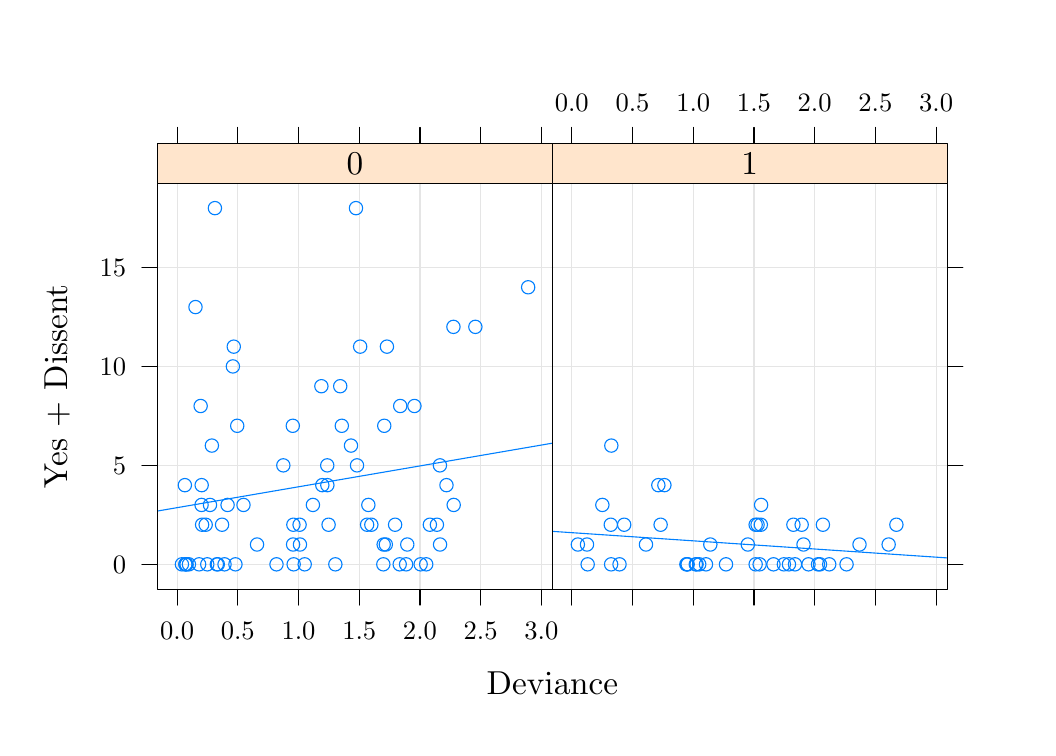
\begin{tikzpicture}[x=1pt,y=1pt]
\definecolor[named]{drawColor}{rgb}{0.00,0.00,0.00}
\definecolor[named]{fillColor}{rgb}{1.00,1.00,1.00}
\fill[color=fillColor,] (0,0) rectangle (361.35,252.94);
\begin{scope}
\path[clip] (  0.00,  0.00) rectangle (361.35,252.94);
\end{scope}
\begin{scope}
\path[clip] (  0.00,  0.00) rectangle (361.35,252.94);

\draw[fill opacity=0.00,draw opacity=0.00,] (  0.00,  0.00) rectangle (361.35,252.94);
\definecolor[named]{drawColor}{rgb}{0.00,0.00,0.00}

\node[color=drawColor,anchor=base,inner sep=0pt, outer sep=0pt, scale=  1.20] at (189.61, 12.04) {Deviance%
};
\end{scope}
\begin{scope}
\path[clip] (  0.00,  0.00) rectangle (361.35,252.94);
\definecolor[named]{drawColor}{rgb}{0.00,0.00,0.00}

\node[rotate= 90.00,color=drawColor,anchor=base,inner sep=0pt, outer sep=0pt, scale=  1.20] at ( 14.29,123.38) {Yes + Dissent%
};
\end{scope}
\begin{scope}
\path[clip] (  0.00,  0.00) rectangle (361.35,252.94);
\end{scope}
\begin{scope}
\path[clip] (  0.00,  0.00) rectangle (361.35,252.94);
\end{scope}
\begin{scope}
\path[clip] (  0.00,  0.00) rectangle (361.35,252.94);
\end{scope}
\begin{scope}
\path[clip] ( 46.98, 50.02) rectangle (189.61,196.74);
\end{scope}
\begin{scope}
\path[clip] (  0.00,  0.00) rectangle (361.35,252.94);
\end{scope}
\begin{scope}
\path[clip] (  0.00,  0.00) rectangle (361.35,252.94);
\definecolor[named]{drawColor}{rgb}{0.00,0.00,0.00}

\draw[color=drawColor,line cap=round,line join=round,fill opacity=0.00,] ( 53.99,211.19) -- ( 53.99,216.88);

\draw[color=drawColor,line cap=round,line join=round,fill opacity=0.00,] ( 75.93,211.19) -- ( 75.93,216.88);

\draw[color=drawColor,line cap=round,line join=round,fill opacity=0.00,] ( 97.87,211.19) -- ( 97.87,216.88);

\draw[color=drawColor,line cap=round,line join=round,fill opacity=0.00,] (119.81,211.19) -- (119.81,216.88);

\draw[color=drawColor,line cap=round,line join=round,fill opacity=0.00,] (141.75,211.19) -- (141.75,216.88);

\draw[color=drawColor,line cap=round,line join=round,fill opacity=0.00,] (163.69,211.19) -- (163.69,216.88);

\draw[color=drawColor,line cap=round,line join=round,fill opacity=0.00,] (185.63,211.19) -- (185.63,216.88);
\end{scope}
\begin{scope}
\path[clip] (  0.00,  0.00) rectangle (361.35,252.94);
\end{scope}
\begin{scope}
\path[clip] (  0.00,  0.00) rectangle (361.35,252.94);
\definecolor[named]{drawColor}{rgb}{0.00,0.00,0.00}

\draw[color=drawColor,line cap=round,line join=round,fill opacity=0.00,] ( 46.98, 59.02) -- ( 41.29, 59.02);

\draw[color=drawColor,line cap=round,line join=round,fill opacity=0.00,] ( 46.98, 94.78) -- ( 41.29, 94.78);

\draw[color=drawColor,line cap=round,line join=round,fill opacity=0.00,] ( 46.98,130.53) -- ( 41.29,130.53);

\draw[color=drawColor,line cap=round,line join=round,fill opacity=0.00,] ( 46.98,166.28) -- ( 41.29,166.28);

\node[color=drawColor,anchor=base east,inner sep=0pt, outer sep=0pt, scale=  0.96] at ( 35.60, 55.72) {0%
};

\node[color=drawColor,anchor=base east,inner sep=0pt, outer sep=0pt, scale=  0.96] at ( 35.60, 91.47) {5%
};

\node[color=drawColor,anchor=base east,inner sep=0pt, outer sep=0pt, scale=  0.96] at ( 35.60,127.22) {10%
};

\node[color=drawColor,anchor=base east,inner sep=0pt, outer sep=0pt, scale=  0.96] at ( 35.60,162.97) {15%
};
\end{scope}
\begin{scope}
\path[clip] (  0.00,  0.00) rectangle (361.35,252.94);
\end{scope}
\begin{scope}
\path[clip] (  0.00,  0.00) rectangle (361.35,252.94);
\definecolor[named]{drawColor}{rgb}{0.00,0.00,0.00}

\draw[color=drawColor,line cap=round,line join=round,fill opacity=0.00,] ( 53.99, 50.02) -- ( 53.99, 44.32);

\draw[color=drawColor,line cap=round,line join=round,fill opacity=0.00,] ( 75.93, 50.02) -- ( 75.93, 44.32);

\draw[color=drawColor,line cap=round,line join=round,fill opacity=0.00,] ( 97.87, 50.02) -- ( 97.87, 44.32);

\draw[color=drawColor,line cap=round,line join=round,fill opacity=0.00,] (119.81, 50.02) -- (119.81, 44.32);

\draw[color=drawColor,line cap=round,line join=round,fill opacity=0.00,] (141.75, 50.02) -- (141.75, 44.32);

\draw[color=drawColor,line cap=round,line join=round,fill opacity=0.00,] (163.69, 50.02) -- (163.69, 44.32);

\draw[color=drawColor,line cap=round,line join=round,fill opacity=0.00,] (185.63, 50.02) -- (185.63, 44.32);

\node[color=drawColor,anchor=base,inner sep=0pt, outer sep=0pt, scale=  0.96] at ( 53.99, 32.02) {0.0%
};

\node[color=drawColor,anchor=base,inner sep=0pt, outer sep=0pt, scale=  0.96] at ( 75.93, 32.02) {0.5%
};

\node[color=drawColor,anchor=base,inner sep=0pt, outer sep=0pt, scale=  0.96] at ( 97.87, 32.02) {1.0%
};

\node[color=drawColor,anchor=base,inner sep=0pt, outer sep=0pt, scale=  0.96] at (119.81, 32.02) {1.5%
};

\node[color=drawColor,anchor=base,inner sep=0pt, outer sep=0pt, scale=  0.96] at (141.75, 32.02) {2.0%
};

\node[color=drawColor,anchor=base,inner sep=0pt, outer sep=0pt, scale=  0.96] at (163.69, 32.02) {2.5%
};

\node[color=drawColor,anchor=base,inner sep=0pt, outer sep=0pt, scale=  0.96] at (185.63, 32.02) {3.0%
};
\end{scope}
\begin{scope}
\path[clip] (  0.00,  0.00) rectangle (361.35,252.94);
\end{scope}
\begin{scope}
\path[clip] ( 46.98, 50.02) rectangle (189.61,196.74);
\definecolor[named]{drawColor}{rgb}{0.90,0.90,0.90}

\draw[color=drawColor,line cap=round,line join=round,fill opacity=0.00,] ( 46.98, 59.02) -- (189.61, 59.02);

\draw[color=drawColor,line cap=round,line join=round,fill opacity=0.00,] ( 46.98, 94.78) -- (189.61, 94.78);

\draw[color=drawColor,line cap=round,line join=round,fill opacity=0.00,] ( 46.98,130.53) -- (189.61,130.53);

\draw[color=drawColor,line cap=round,line join=round,fill opacity=0.00,] ( 46.98,166.28) -- (189.61,166.28);

\draw[color=drawColor,line cap=round,line join=round,fill opacity=0.00,] ( 53.99, 50.02) -- ( 53.99,196.74);

\draw[color=drawColor,line cap=round,line join=round,fill opacity=0.00,] ( 75.93, 50.02) -- ( 75.93,196.74);

\draw[color=drawColor,line cap=round,line join=round,fill opacity=0.00,] ( 97.87, 50.02) -- ( 97.87,196.74);

\draw[color=drawColor,line cap=round,line join=round,fill opacity=0.00,] (119.81, 50.02) -- (119.81,196.74);

\draw[color=drawColor,line cap=round,line join=round,fill opacity=0.00,] (141.75, 50.02) -- (141.75,196.74);

\draw[color=drawColor,line cap=round,line join=round,fill opacity=0.00,] (163.69, 50.02) -- (163.69,196.74);

\draw[color=drawColor,line cap=round,line join=round,fill opacity=0.00,] (185.63, 50.02) -- (185.63,196.74);
\definecolor[named]{drawColor}{rgb}{0.00,0.50,1.00}

\draw[color=drawColor,line cap=round,line join=round,fill opacity=0.00,] ( 71.13, 59.02) circle (  2.41);

\draw[color=drawColor,line cap=round,line join=round,fill opacity=0.00,] ( 72.23, 80.48) circle (  2.41);

\draw[color=drawColor,line cap=round,line join=round,fill opacity=0.00,] ( 75.08, 59.02) circle (  2.41);

\draw[color=drawColor,line cap=round,line join=round,fill opacity=0.00,] (148.97, 94.78) circle (  2.41);

\draw[color=drawColor,line cap=round,line join=round,fill opacity=0.00,] ( 77.98, 80.48) circle (  2.41);

\draw[color=drawColor,line cap=round,line join=round,fill opacity=0.00,] (122.66, 73.33) circle (  2.41);

\draw[color=drawColor,line cap=round,line join=round,fill opacity=0.00,] ( 98.25, 73.33) circle (  2.41);

\draw[color=drawColor,line cap=round,line join=round,fill opacity=0.00,] ( 57.07, 59.02) circle (  2.41);

\draw[color=drawColor,line cap=round,line join=round,fill opacity=0.00,] ( 61.95, 59.02) circle (  2.41);

\draw[color=drawColor,line cap=round,line join=round,fill opacity=0.00,] ( 64.90, 59.02) circle (  2.41);

\draw[color=drawColor,line cap=round,line join=round,fill opacity=0.00,] ( 95.80,109.08) circle (  2.41);

\draw[color=drawColor,line cap=round,line join=round,fill opacity=0.00,] ( 75.72,109.08) circle (  2.41);

\draw[color=drawColor,line cap=round,line join=round,fill opacity=0.00,] ( 65.88, 80.48) circle (  2.41);

\draw[color=drawColor,line cap=round,line join=round,fill opacity=0.00,] ( 68.70, 59.02) circle (  2.41);

\draw[color=drawColor,line cap=round,line join=round,fill opacity=0.00,] (120.14,137.68) circle (  2.41);

\draw[color=drawColor,line cap=round,line join=round,fill opacity=0.00,] (134.62,116.23) circle (  2.41);

\draw[color=drawColor,line cap=round,line join=round,fill opacity=0.00,] (132.77, 73.33) circle (  2.41);

\draw[color=drawColor,line cap=round,line join=round,fill opacity=0.00,] (134.43, 59.02) circle (  2.41);

\draw[color=drawColor,line cap=round,line join=round,fill opacity=0.00,] ( 66.56,101.93) circle (  2.41);

\draw[color=drawColor,line cap=round,line join=round,fill opacity=0.00,] ( 82.88, 66.18) circle (  2.41);

\draw[color=drawColor,line cap=round,line join=round,fill opacity=0.00,] ( 58.27, 59.02) circle (  2.41);

\draw[color=drawColor,line cap=round,line join=round,fill opacity=0.00,] ( 64.32, 73.33) circle (  2.41);

\draw[color=drawColor,line cap=round,line join=round,fill opacity=0.00,] ( 96.11, 59.02) circle (  2.41);

\draw[color=drawColor,line cap=round,line join=round,fill opacity=0.00,] ( 70.24, 73.33) circle (  2.41);

\draw[color=drawColor,line cap=round,line join=round,fill opacity=0.00,] ( 68.35, 59.02) circle (  2.41);

\draw[color=drawColor,line cap=round,line join=round,fill opacity=0.00,] (142.00, 59.02) circle (  2.41);

\draw[color=drawColor,line cap=round,line join=round,fill opacity=0.00,] (145.33, 73.33) circle (  2.41);

\draw[color=drawColor,line cap=round,line join=round,fill opacity=0.00,] (151.33, 87.63) circle (  2.41);

\draw[color=drawColor,line cap=round,line join=round,fill opacity=0.00,] (100.10, 59.02) circle (  2.41);

\draw[color=drawColor,line cap=round,line join=round,fill opacity=0.00,] ( 96.01, 73.33) circle (  2.41);

\draw[color=drawColor,line cap=round,line join=round,fill opacity=0.00,] (106.46, 87.63) circle (  2.41);

\draw[color=drawColor,line cap=round,line join=round,fill opacity=0.00,] (116.83,101.93) circle (  2.41);

\draw[color=drawColor,line cap=round,line join=round,fill opacity=0.00,] ( 67.66,187.73) circle (  2.41);

\draw[color=drawColor,line cap=round,line join=round,fill opacity=0.00,] (129.82,137.68) circle (  2.41);

\draw[color=drawColor,line cap=round,line join=round,fill opacity=0.00,] (161.77,144.83) circle (  2.41);

\draw[color=drawColor,line cap=round,line join=round,fill opacity=0.00,] ( 95.91, 66.18) circle (  2.41);

\draw[color=drawColor,line cap=round,line join=round,fill opacity=0.00,] ( 98.39, 66.18) circle (  2.41);

\draw[color=drawColor,line cap=round,line join=round,fill opacity=0.00,] ( 62.87, 87.63) circle (  2.41);

\draw[color=drawColor,line cap=round,line join=round,fill opacity=0.00,] (103.07, 80.48) circle (  2.41);

\draw[color=drawColor,line cap=round,line join=round,fill opacity=0.00,] (149.01, 66.18) circle (  2.41);

\draw[color=drawColor,line cap=round,line join=round,fill opacity=0.00,] (113.51,109.08) circle (  2.41);

\draw[color=drawColor,line cap=round,line join=round,fill opacity=0.00,] ( 56.97, 59.02) circle (  2.41);

\draw[color=drawColor,line cap=round,line join=round,fill opacity=0.00,] ( 55.74, 59.02) circle (  2.41);

\draw[color=drawColor,line cap=round,line join=round,fill opacity=0.00,] (147.88, 73.33) circle (  2.41);

\draw[color=drawColor,line cap=round,line join=round,fill opacity=0.00,] (119.01, 94.78) circle (  2.41);

\draw[color=drawColor,line cap=round,line join=round,fill opacity=0.00,] (129.41, 66.18) circle (  2.41);

\draw[color=drawColor,line cap=round,line join=round,fill opacity=0.00,] (136.74, 59.02) circle (  2.41);

\draw[color=drawColor,line cap=round,line join=round,fill opacity=0.00,] (137.17, 66.18) circle (  2.41);

\draw[color=drawColor,line cap=round,line join=round,fill opacity=0.00,] (144.01, 59.02) circle (  2.41);

\draw[color=drawColor,line cap=round,line join=round,fill opacity=0.00,] (153.94, 80.48) circle (  2.41);

\draw[color=drawColor,line cap=round,line join=round,fill opacity=0.00,] ( 89.91, 59.02) circle (  2.41);

\draw[color=drawColor,line cap=round,line join=round,fill opacity=0.00,] (123.10, 80.48) circle (  2.41);

\draw[color=drawColor,line cap=round,line join=round,fill opacity=0.00,] ( 56.80, 87.63) circle (  2.41);

\draw[color=drawColor,line cap=round,line join=round,fill opacity=0.00,] ( 57.42, 59.02) circle (  2.41);

\draw[color=drawColor,line cap=round,line join=round,fill opacity=0.00,] (111.18, 59.02) circle (  2.41);

\draw[color=drawColor,line cap=round,line join=round,fill opacity=0.00,] ( 62.50,116.23) circle (  2.41);

\draw[color=drawColor,line cap=round,line join=round,fill opacity=0.00,] ( 63.03, 73.33) circle (  2.41);

\draw[color=drawColor,line cap=round,line join=round,fill opacity=0.00,] ( 62.83, 80.48) circle (  2.41);

\draw[color=drawColor,line cap=round,line join=round,fill opacity=0.00,] ( 60.64,151.98) circle (  2.41);

\draw[color=drawColor,line cap=round,line join=round,fill opacity=0.00,] (108.25, 94.78) circle (  2.41);

\draw[color=drawColor,line cap=round,line join=round,fill opacity=0.00,] ( 74.15,130.53) circle (  2.41);

\draw[color=drawColor,line cap=round,line join=round,fill opacity=0.00,] ( 92.38, 94.78) circle (  2.41);

\draw[color=drawColor,line cap=round,line join=round,fill opacity=0.00,] (128.64, 66.18) circle (  2.41);

\draw[color=drawColor,line cap=round,line join=round,fill opacity=0.00,] (112.94,123.38) circle (  2.41);

\draw[color=drawColor,line cap=round,line join=round,fill opacity=0.00,] (180.85,159.13) circle (  2.41);

\draw[color=drawColor,line cap=round,line join=round,fill opacity=0.00,] (139.75,116.23) circle (  2.41);

\draw[color=drawColor,line cap=round,line join=round,fill opacity=0.00,] (128.85,109.08) circle (  2.41);

\draw[color=drawColor,line cap=round,line join=round,fill opacity=0.00,] (128.51, 59.02) circle (  2.41);

\draw[color=drawColor,line cap=round,line join=round,fill opacity=0.00,] (124.18, 73.33) circle (  2.41);

\draw[color=drawColor,line cap=round,line join=round,fill opacity=0.00,] (153.85,144.83) circle (  2.41);

\draw[color=drawColor,line cap=round,line join=round,fill opacity=0.00,] (108.73, 73.33) circle (  2.41);

\draw[color=drawColor,line cap=round,line join=round,fill opacity=0.00,] ( 74.47,137.68) circle (  2.41);

\draw[color=drawColor,line cap=round,line join=round,fill opacity=0.00,] (118.63,187.73) circle (  2.41);

\draw[color=drawColor,line cap=round,line join=round,fill opacity=0.00,] (106.13,123.38) circle (  2.41);

\draw[color=drawColor,line cap=round,line join=round,fill opacity=0.00,] (108.29, 87.63) circle (  2.41);

\draw[color=drawColor,line cap=round,line join=round,fill opacity=0.00,] (189.61,102.80) --
	( 46.98, 78.29);
\end{scope}
\begin{scope}
\path[clip] (  0.00,  0.00) rectangle (361.35,252.94);
\end{scope}
\begin{scope}
\path[clip] (  0.00,  0.00) rectangle (361.35,252.94);
\definecolor[named]{drawColor}{rgb}{0.00,0.00,0.00}

\draw[color=drawColor,line cap=round,line join=round,fill opacity=0.00,] ( 46.98, 50.02) rectangle (189.61,196.74);
\end{scope}
\begin{scope}
\path[clip] (  0.00,  0.00) rectangle (361.35,252.94);
\end{scope}
\begin{scope}
\path[clip] (  0.00,  0.00) rectangle (361.35,252.94);
\end{scope}
\begin{scope}
\path[clip] ( 46.98,196.74) rectangle (189.61,211.19);
\definecolor[named]{drawColor}{rgb}{1.00,0.90,0.80}
\definecolor[named]{fillColor}{rgb}{1.00,0.90,0.80}

\draw[color=drawColor,line cap=round,line join=round,fill=fillColor,] ( 46.98,196.74) rectangle (189.61,211.19);
\definecolor[named]{drawColor}{rgb}{0.00,0.00,0.00}

\node[color=drawColor,anchor=base west,inner sep=0pt, outer sep=0pt, scale=  1.20] at (115.29,199.83) {0%
};
\end{scope}
\begin{scope}
\path[clip] (  0.00,  0.00) rectangle (361.35,252.94);
\end{scope}
\begin{scope}
\path[clip] (  0.00,  0.00) rectangle (361.35,252.94);
\definecolor[named]{drawColor}{rgb}{0.00,0.00,0.00}

\draw[color=drawColor,line cap=round,line join=round,fill opacity=0.00,] ( 46.98,196.74) rectangle (189.61,211.19);
\end{scope}
\begin{scope}
\path[clip] (  0.00,  0.00) rectangle (361.35,252.94);
\end{scope}
\begin{scope}
\path[clip] (  0.00,  0.00) rectangle (361.35,252.94);
\end{scope}
\begin{scope}
\path[clip] (189.61, 50.02) rectangle (332.23,196.74);
\end{scope}
\begin{scope}
\path[clip] (  0.00,  0.00) rectangle (361.35,252.94);
\end{scope}
\begin{scope}
\path[clip] (  0.00,  0.00) rectangle (361.35,252.94);
\definecolor[named]{drawColor}{rgb}{0.00,0.00,0.00}

\draw[color=drawColor,line cap=round,line join=round,fill opacity=0.00,] (196.62,211.19) -- (196.62,216.88);

\draw[color=drawColor,line cap=round,line join=round,fill opacity=0.00,] (218.56,211.19) -- (218.56,216.88);

\draw[color=drawColor,line cap=round,line join=round,fill opacity=0.00,] (240.50,211.19) -- (240.50,216.88);

\draw[color=drawColor,line cap=round,line join=round,fill opacity=0.00,] (262.44,211.19) -- (262.44,216.88);

\draw[color=drawColor,line cap=round,line join=round,fill opacity=0.00,] (284.38,211.19) -- (284.38,216.88);

\draw[color=drawColor,line cap=round,line join=round,fill opacity=0.00,] (306.32,211.19) -- (306.32,216.88);

\draw[color=drawColor,line cap=round,line join=round,fill opacity=0.00,] (328.25,211.19) -- (328.25,216.88);

\node[color=drawColor,anchor=base,inner sep=0pt, outer sep=0pt, scale=  0.96] at (196.62,222.58) {0.0%
};

\node[color=drawColor,anchor=base,inner sep=0pt, outer sep=0pt, scale=  0.96] at (218.56,222.58) {0.5%
};

\node[color=drawColor,anchor=base,inner sep=0pt, outer sep=0pt, scale=  0.96] at (240.50,222.58) {1.0%
};

\node[color=drawColor,anchor=base,inner sep=0pt, outer sep=0pt, scale=  0.96] at (262.44,222.58) {1.5%
};

\node[color=drawColor,anchor=base,inner sep=0pt, outer sep=0pt, scale=  0.96] at (284.38,222.58) {2.0%
};

\node[color=drawColor,anchor=base,inner sep=0pt, outer sep=0pt, scale=  0.96] at (306.32,222.58) {2.5%
};

\node[color=drawColor,anchor=base,inner sep=0pt, outer sep=0pt, scale=  0.96] at (328.25,222.58) {3.0%
};
\end{scope}
\begin{scope}
\path[clip] (  0.00,  0.00) rectangle (361.35,252.94);
\end{scope}
\begin{scope}
\path[clip] (  0.00,  0.00) rectangle (361.35,252.94);
\end{scope}
\begin{scope}
\path[clip] (  0.00,  0.00) rectangle (361.35,252.94);
\end{scope}
\begin{scope}
\path[clip] (  0.00,  0.00) rectangle (361.35,252.94);
\definecolor[named]{drawColor}{rgb}{0.00,0.00,0.00}

\draw[color=drawColor,line cap=round,line join=round,fill opacity=0.00,] (196.62, 50.02) -- (196.62, 44.32);

\draw[color=drawColor,line cap=round,line join=round,fill opacity=0.00,] (218.56, 50.02) -- (218.56, 44.32);

\draw[color=drawColor,line cap=round,line join=round,fill opacity=0.00,] (240.50, 50.02) -- (240.50, 44.32);

\draw[color=drawColor,line cap=round,line join=round,fill opacity=0.00,] (262.44, 50.02) -- (262.44, 44.32);

\draw[color=drawColor,line cap=round,line join=round,fill opacity=0.00,] (284.38, 50.02) -- (284.38, 44.32);

\draw[color=drawColor,line cap=round,line join=round,fill opacity=0.00,] (306.32, 50.02) -- (306.32, 44.32);

\draw[color=drawColor,line cap=round,line join=round,fill opacity=0.00,] (328.25, 50.02) -- (328.25, 44.32);

\draw[color=drawColor,line cap=round,line join=round,fill opacity=0.00,] (332.23, 59.02) -- (337.92, 59.02);

\draw[color=drawColor,line cap=round,line join=round,fill opacity=0.00,] (332.23, 94.78) -- (337.92, 94.78);

\draw[color=drawColor,line cap=round,line join=round,fill opacity=0.00,] (332.23,130.53) -- (337.92,130.53);

\draw[color=drawColor,line cap=round,line join=round,fill opacity=0.00,] (332.23,166.28) -- (337.92,166.28);
\end{scope}
\begin{scope}
\path[clip] (  0.00,  0.00) rectangle (361.35,252.94);
\end{scope}
\begin{scope}
\path[clip] (189.61, 50.02) rectangle (332.23,196.74);
\definecolor[named]{drawColor}{rgb}{0.90,0.90,0.90}

\draw[color=drawColor,line cap=round,line join=round,fill opacity=0.00,] (189.61, 59.02) -- (332.23, 59.02);

\draw[color=drawColor,line cap=round,line join=round,fill opacity=0.00,] (189.61, 94.78) -- (332.23, 94.78);

\draw[color=drawColor,line cap=round,line join=round,fill opacity=0.00,] (189.61,130.53) -- (332.23,130.53);

\draw[color=drawColor,line cap=round,line join=round,fill opacity=0.00,] (189.61,166.28) -- (332.23,166.28);

\draw[color=drawColor,line cap=round,line join=round,fill opacity=0.00,] (196.62, 50.02) -- (196.62,196.74);

\draw[color=drawColor,line cap=round,line join=round,fill opacity=0.00,] (218.56, 50.02) -- (218.56,196.74);

\draw[color=drawColor,line cap=round,line join=round,fill opacity=0.00,] (240.50, 50.02) -- (240.50,196.74);

\draw[color=drawColor,line cap=round,line join=round,fill opacity=0.00,] (262.44, 50.02) -- (262.44,196.74);

\draw[color=drawColor,line cap=round,line join=round,fill opacity=0.00,] (284.38, 50.02) -- (284.38,196.74);

\draw[color=drawColor,line cap=round,line join=round,fill opacity=0.00,] (306.32, 50.02) -- (306.32,196.74);

\draw[color=drawColor,line cap=round,line join=round,fill opacity=0.00,] (328.25, 50.02) -- (328.25,196.74);
\definecolor[named]{drawColor}{rgb}{0.00,0.50,1.00}

\draw[color=drawColor,line cap=round,line join=round,fill opacity=0.00,] (238.49, 59.02) circle (  2.41);

\draw[color=drawColor,line cap=round,line join=round,fill opacity=0.00,] (287.35, 73.33) circle (  2.41);

\draw[color=drawColor,line cap=round,line join=round,fill opacity=0.00,] (265.02, 80.48) circle (  2.41);

\draw[color=drawColor,line cap=round,line join=round,fill opacity=0.00,] (241.71, 59.02) circle (  2.41);

\draw[color=drawColor,line cap=round,line join=round,fill opacity=0.00,] (202.11, 66.18) circle (  2.41);

\draw[color=drawColor,line cap=round,line join=round,fill opacity=0.00,] (198.81, 66.18) circle (  2.41);

\draw[color=drawColor,line cap=round,line join=round,fill opacity=0.00,] (202.35, 59.02) circle (  2.41);

\draw[color=drawColor,line cap=round,line join=round,fill opacity=0.00,] (275.09, 59.02) circle (  2.41);

\draw[color=drawColor,line cap=round,line join=round,fill opacity=0.00,] (223.42, 66.18) circle (  2.41);

\draw[color=drawColor,line cap=round,line join=round,fill opacity=0.00,] (210.90,101.93) circle (  2.41);

\draw[color=drawColor,line cap=round,line join=round,fill opacity=0.00,] (242.67, 59.02) circle (  2.41);

\draw[color=drawColor,line cap=round,line join=round,fill opacity=0.00,] (295.90, 59.02) circle (  2.41);

\draw[color=drawColor,line cap=round,line join=round,fill opacity=0.00,] (246.67, 66.18) circle (  2.41);

\draw[color=drawColor,line cap=round,line join=round,fill opacity=0.00,] (311.11, 66.18) circle (  2.41);

\draw[color=drawColor,line cap=round,line join=round,fill opacity=0.00,] (285.58, 59.02) circle (  2.41);

\draw[color=drawColor,line cap=round,line join=round,fill opacity=0.00,] (313.91, 73.33) circle (  2.41);

\draw[color=drawColor,line cap=round,line join=round,fill opacity=0.00,] (280.35, 66.18) circle (  2.41);

\draw[color=drawColor,line cap=round,line join=round,fill opacity=0.00,] (282.15, 59.02) circle (  2.41);

\draw[color=drawColor,line cap=round,line join=round,fill opacity=0.00,] (264.92, 73.33) circle (  2.41);

\draw[color=drawColor,line cap=round,line join=round,fill opacity=0.00,] (238.02, 59.02) circle (  2.41);

\draw[color=drawColor,line cap=round,line join=round,fill opacity=0.00,] (263.74, 73.33) circle (  2.41);

\draw[color=drawColor,line cap=round,line join=round,fill opacity=0.00,] (245.11, 59.02) circle (  2.41);

\draw[color=drawColor,line cap=round,line join=round,fill opacity=0.00,] (238.24, 59.02) circle (  2.41);

\draw[color=drawColor,line cap=round,line join=round,fill opacity=0.00,] (263.05, 59.02) circle (  2.41);

\draw[color=drawColor,line cap=round,line join=round,fill opacity=0.00,] (264.49, 59.02) circle (  2.41);

\draw[color=drawColor,line cap=round,line join=round,fill opacity=0.00,] (263.05, 73.33) circle (  2.41);

\draw[color=drawColor,line cap=round,line join=round,fill opacity=0.00,] (269.49, 59.02) circle (  2.41);

\draw[color=drawColor,line cap=round,line join=round,fill opacity=0.00,] (210.70, 73.33) circle (  2.41);

\draw[color=drawColor,line cap=round,line join=round,fill opacity=0.00,] (289.64, 59.02) circle (  2.41);

\draw[color=drawColor,line cap=round,line join=round,fill opacity=0.00,] (227.89, 87.63) circle (  2.41);

\draw[color=drawColor,line cap=round,line join=round,fill opacity=0.00,] (230.08, 87.63) circle (  2.41);

\draw[color=drawColor,line cap=round,line join=round,fill opacity=0.00,] (279.68, 73.33) circle (  2.41);

\draw[color=drawColor,line cap=round,line join=round,fill opacity=0.00,] (276.69, 73.33) circle (  2.41);

\draw[color=drawColor,line cap=round,line join=round,fill opacity=0.00,] (300.58, 66.18) circle (  2.41);

\draw[color=drawColor,line cap=round,line join=round,fill opacity=0.00,] (286.30, 59.02) circle (  2.41);

\draw[color=drawColor,line cap=round,line join=round,fill opacity=0.00,] (207.66, 80.48) circle (  2.41);

\draw[color=drawColor,line cap=round,line join=round,fill opacity=0.00,] (241.42, 59.02) circle (  2.41);

\draw[color=drawColor,line cap=round,line join=round,fill opacity=0.00,] (210.83, 59.02) circle (  2.41);

\draw[color=drawColor,line cap=round,line join=round,fill opacity=0.00,] (213.86, 59.02) circle (  2.41);

\draw[color=drawColor,line cap=round,line join=round,fill opacity=0.00,] (260.22, 66.18) circle (  2.41);

\draw[color=drawColor,line cap=round,line join=round,fill opacity=0.00,] (252.34, 59.02) circle (  2.41);

\draw[color=drawColor,line cap=round,line join=round,fill opacity=0.00,] (215.55, 73.33) circle (  2.41);

\draw[color=drawColor,line cap=round,line join=round,fill opacity=0.00,] (228.71, 73.33) circle (  2.41);

\draw[color=drawColor,line cap=round,line join=round,fill opacity=0.00,] (277.27, 59.02) circle (  2.41);

\draw[color=drawColor,line cap=round,line join=round,fill opacity=0.00,] (273.25, 59.02) circle (  2.41);

\draw[color=drawColor,line cap=round,line join=round,fill opacity=0.00,] (332.23, 61.34) --
	(189.61, 70.93);
\end{scope}
\begin{scope}
\path[clip] (  0.00,  0.00) rectangle (361.35,252.94);
\end{scope}
\begin{scope}
\path[clip] (  0.00,  0.00) rectangle (361.35,252.94);
\definecolor[named]{drawColor}{rgb}{0.00,0.00,0.00}

\draw[color=drawColor,line cap=round,line join=round,fill opacity=0.00,] (189.61, 50.02) rectangle (332.23,196.74);
\end{scope}
\begin{scope}
\path[clip] (  0.00,  0.00) rectangle (361.35,252.94);
\end{scope}
\begin{scope}
\path[clip] (  0.00,  0.00) rectangle (361.35,252.94);
\end{scope}
\begin{scope}
\path[clip] (189.61,196.74) rectangle (332.23,211.19);
\definecolor[named]{drawColor}{rgb}{1.00,0.90,0.80}
\definecolor[named]{fillColor}{rgb}{1.00,0.90,0.80}

\draw[color=drawColor,line cap=round,line join=round,fill=fillColor,] (189.61,196.74) rectangle (332.23,211.19);
\definecolor[named]{drawColor}{rgb}{0.00,0.00,0.00}

\node[color=drawColor,anchor=base west,inner sep=0pt, outer sep=0pt, scale=  1.20] at (257.92,199.83) {1%
};
\end{scope}
\begin{scope}
\path[clip] (  0.00,  0.00) rectangle (361.35,252.94);
\end{scope}
\begin{scope}
\path[clip] (  0.00,  0.00) rectangle (361.35,252.94);
\definecolor[named]{drawColor}{rgb}{0.00,0.00,0.00}

\draw[color=drawColor,line cap=round,line join=round,fill opacity=0.00,] (189.61,196.74) rectangle (332.23,211.19);
\end{scope}
\begin{scope}
\path[clip] (  0.00,  0.00) rectangle (361.35,252.94);
\end{scope}
\begin{scope}
\path[clip] (  0.00,  0.00) rectangle (361.35,252.94);
\end{scope}
\begin{scope}
\path[clip] (  0.00,  0.00) rectangle (361.35,252.94);
\end{scope}
\begin{scope}
\path[clip] (  0.00,  0.00) rectangle (361.35,252.94);
\end{scope}
\end{tikzpicture}
}}\quad
\caption{The plot show the squared deviance from the mean left-right position in the Council on the x-axis, and the number of abstentions on the y-axis. The values have been conditioned on whether a government was from an old or new member state.}
\label{fig:scatter}
\end{figure}

Consistently across all categories we see a positive relationship between deviance and the number of dissenting votes for old member states, and the opposite, although very weak, relationship for new member states. The plots show a somewhat surprising result as most of the literature on the Council show that there was no large effect of the eastern enlargement, but there does seem to be quite a large difference in voting behavior between governments from new and old member states. Hypothesis two is partly supported by Figure \ref{fig:scatter}, but only for old member states. New member states do not engage in dissenting behavior to the same extent as old member states, the modus operandi seem to be supportive of the outcome of Council negotiations, regardless of how much the deviate from the Council mean left-right position. Panel (b) in Figure \ref{fig:scatter} is not entirely expected, as the theory of diffuse reciprocity do not link no votes to being an outlier within in the Council, they are supposed to signal back home, despite that a government might be in favor of a dossier. One should be careful in interpreting the figures, though, as we cannot know how many cases there were an overlap of an outlying government that was also under domestic pressure to resist the result of the Council negotiations. We also see that yes votes with a dissenting statement increase as a government becomes more of an outlier in the Council, this is also what we would expect as in these instances the norm of diffuse reciprocity should be effective.  

The examine hypothesis three initially presents some obstacles. To avoid the effect of time, i.e. the longer a government has been in the Council the more likely it is to have cast a dissenting vote, the number of votes in a given choice category relative to the time spend in the Council were plotted, conditioned on the time spend in the council. The y-axis show the density within each category, while the x-axis show the relative voting frequency.

 
\begin{figure}[htp]
\centering
\scalebox{.6}{\subfloat[][No Votes]{% Created by tikzDevice version 0.6.1 on 2011-07-24 21:12:39
% !TEX encoding = UTF-8 Unicode
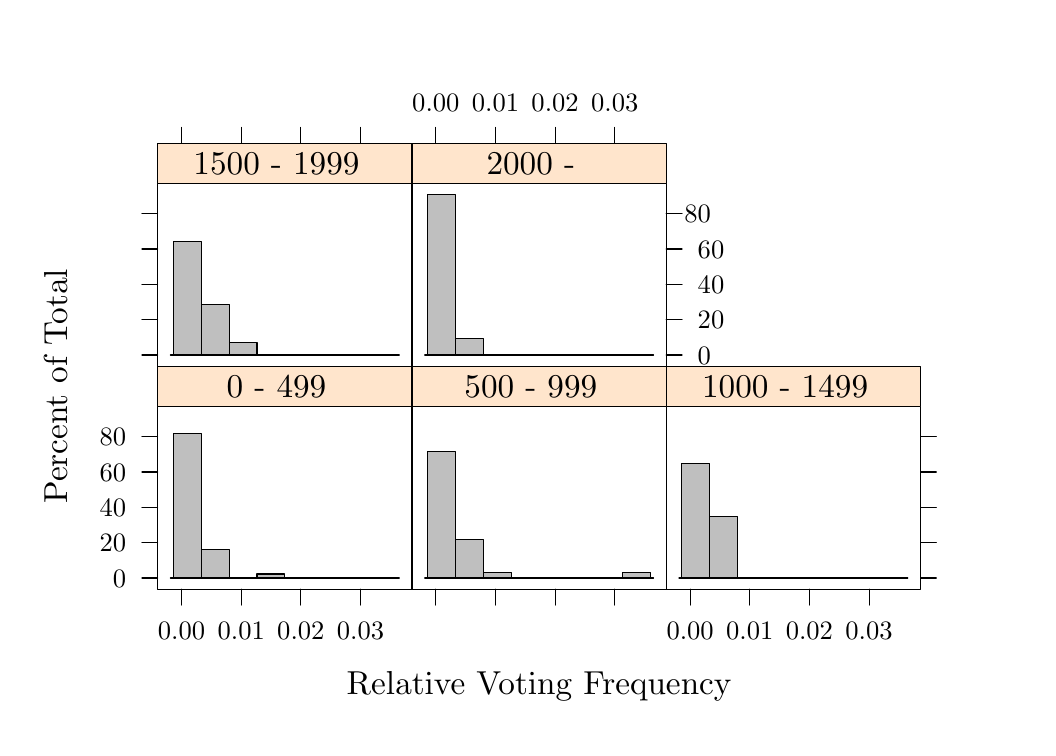
\begin{tikzpicture}[x=1pt,y=1pt]
\definecolor[named]{drawColor}{rgb}{0.00,0.00,0.00}
\definecolor[named]{fillColor}{rgb}{1.00,1.00,1.00}
\fill[color=fillColor,] (0,0) rectangle (361.35,252.94);
\begin{scope}
\path[clip] (  0.00,  0.00) rectangle (361.35,252.94);
\end{scope}
\begin{scope}
\path[clip] (  0.00,  0.00) rectangle (361.35,252.94);

\draw[fill opacity=0.00,draw opacity=0.00,] (  0.00,  0.00) rectangle (361.35,252.94);
\definecolor[named]{drawColor}{rgb}{0.00,0.00,0.00}

\node[color=drawColor,anchor=base,inner sep=0pt, outer sep=0pt, scale=  1.20] at (184.81, 12.04) {Relative Voting Frequency%
};
\end{scope}
\begin{scope}
\path[clip] (  0.00,  0.00) rectangle (361.35,252.94);
\definecolor[named]{drawColor}{rgb}{0.00,0.00,0.00}

\node[rotate= 90.00,color=drawColor,anchor=base,inner sep=0pt, outer sep=0pt, scale=  1.20] at ( 14.29,123.38) {Percent of Total%
};
\end{scope}
\begin{scope}
\path[clip] (  0.00,  0.00) rectangle (361.35,252.94);
\end{scope}
\begin{scope}
\path[clip] (  0.00,  0.00) rectangle (361.35,252.94);
\end{scope}
\begin{scope}
\path[clip] (  0.00,  0.00) rectangle (361.35,252.94);
\end{scope}
\begin{scope}
\path[clip] ( 46.98, 50.02) rectangle (138.86,116.15);
\end{scope}
\begin{scope}
\path[clip] (  0.00,  0.00) rectangle (361.35,252.94);
\end{scope}
\begin{scope}
\path[clip] (  0.00,  0.00) rectangle (361.35,252.94);
\end{scope}
\begin{scope}
\path[clip] (  0.00,  0.00) rectangle (361.35,252.94);
\end{scope}
\begin{scope}
\path[clip] (  0.00,  0.00) rectangle (361.35,252.94);
\definecolor[named]{drawColor}{rgb}{0.00,0.00,0.00}

\draw[color=drawColor,line cap=round,line join=round,fill opacity=0.00,] ( 46.98, 54.08) -- ( 41.29, 54.08);

\draw[color=drawColor,line cap=round,line join=round,fill opacity=0.00,] ( 46.98, 66.84) -- ( 41.29, 66.84);

\draw[color=drawColor,line cap=round,line join=round,fill opacity=0.00,] ( 46.98, 79.60) -- ( 41.29, 79.60);

\draw[color=drawColor,line cap=round,line join=round,fill opacity=0.00,] ( 46.98, 92.37) -- ( 41.29, 92.37);

\draw[color=drawColor,line cap=round,line join=round,fill opacity=0.00,] ( 46.98,105.13) -- ( 41.29,105.13);

\node[color=drawColor,anchor=base east,inner sep=0pt, outer sep=0pt, scale=  0.96] at ( 35.60, 50.77) {0%
};

\node[color=drawColor,anchor=base east,inner sep=0pt, outer sep=0pt, scale=  0.96] at ( 35.60, 63.53) {20%
};

\node[color=drawColor,anchor=base east,inner sep=0pt, outer sep=0pt, scale=  0.96] at ( 35.60, 76.30) {40%
};

\node[color=drawColor,anchor=base east,inner sep=0pt, outer sep=0pt, scale=  0.96] at ( 35.60, 89.06) {60%
};

\node[color=drawColor,anchor=base east,inner sep=0pt, outer sep=0pt, scale=  0.96] at ( 35.60,101.82) {80%
};
\end{scope}
\begin{scope}
\path[clip] (  0.00,  0.00) rectangle (361.35,252.94);
\end{scope}
\begin{scope}
\path[clip] (  0.00,  0.00) rectangle (361.35,252.94);
\definecolor[named]{drawColor}{rgb}{0.00,0.00,0.00}

\draw[color=drawColor,line cap=round,line join=round,fill opacity=0.00,] ( 55.61, 50.02) -- ( 55.61, 44.32);

\draw[color=drawColor,line cap=round,line join=round,fill opacity=0.00,] ( 77.16, 50.02) -- ( 77.16, 44.32);

\draw[color=drawColor,line cap=round,line join=round,fill opacity=0.00,] ( 98.71, 50.02) -- ( 98.71, 44.32);

\draw[color=drawColor,line cap=round,line join=round,fill opacity=0.00,] (120.26, 50.02) -- (120.26, 44.32);

\node[color=drawColor,anchor=base,inner sep=0pt, outer sep=0pt, scale=  0.96] at ( 55.61, 32.02) {0.00%
};

\node[color=drawColor,anchor=base,inner sep=0pt, outer sep=0pt, scale=  0.96] at ( 77.16, 32.02) {0.01%
};

\node[color=drawColor,anchor=base,inner sep=0pt, outer sep=0pt, scale=  0.96] at ( 98.71, 32.02) {0.02%
};

\node[color=drawColor,anchor=base,inner sep=0pt, outer sep=0pt, scale=  0.96] at (120.26, 32.02) {0.03%
};
\end{scope}
\begin{scope}
\path[clip] (  0.00,  0.00) rectangle (361.35,252.94);
\end{scope}
\begin{scope}
\path[clip] ( 46.98, 50.02) rectangle (138.86,116.15);
\definecolor[named]{drawColor}{rgb}{0.00,0.00,0.00}

\draw[color=drawColor,line cap=round,line join=round,fill opacity=0.00,] ( 51.57, 54.08) --
	(134.27, 54.08);
\definecolor[named]{fillColor}{rgb}{0.75,0.75,0.75}

\draw[color=drawColor,line cap=round,line join=round,fill=fillColor,] ( 52.62, 54.08) rectangle ( 62.70,106.29);

\draw[color=drawColor,line cap=round,line join=round,fill=fillColor,] ( 62.70, 54.08) rectangle ( 72.77, 64.23);

\draw[color=drawColor,line cap=round,line join=round,fill=fillColor,] ( 72.77, 54.08) rectangle ( 82.85, 54.08);

\draw[color=drawColor,line cap=round,line join=round,fill=fillColor,] ( 82.85, 54.08) rectangle ( 92.92, 55.53);

\draw[color=drawColor,line cap=round,line join=round,fill=fillColor,] ( 92.92, 54.08) rectangle (103.00, 54.08);

\draw[color=drawColor,line cap=round,line join=round,fill=fillColor,] (103.00, 54.08) rectangle (113.07, 54.08);

\draw[color=drawColor,line cap=round,line join=round,fill=fillColor,] (113.07, 54.08) rectangle (123.15, 54.08);

\draw[color=drawColor,line cap=round,line join=round,fill=fillColor,] (123.15, 54.08) rectangle (133.22, 54.08);
\end{scope}
\begin{scope}
\path[clip] (  0.00,  0.00) rectangle (361.35,252.94);
\end{scope}
\begin{scope}
\path[clip] (  0.00,  0.00) rectangle (361.35,252.94);
\definecolor[named]{drawColor}{rgb}{0.00,0.00,0.00}

\draw[color=drawColor,line cap=round,line join=round,fill opacity=0.00,] ( 46.98, 50.02) rectangle (138.86,116.15);
\end{scope}
\begin{scope}
\path[clip] (  0.00,  0.00) rectangle (361.35,252.94);
\end{scope}
\begin{scope}
\path[clip] (  0.00,  0.00) rectangle (361.35,252.94);
\end{scope}
\begin{scope}
\path[clip] ( 46.98,116.15) rectangle (138.86,130.60);
\definecolor[named]{drawColor}{rgb}{1.00,0.90,0.80}
\definecolor[named]{fillColor}{rgb}{1.00,0.90,0.80}

\draw[color=drawColor,line cap=round,line join=round,fill=fillColor,] ( 46.98,116.15) rectangle (138.86,130.60);
\definecolor[named]{drawColor}{rgb}{0.00,0.00,0.00}

\node[color=drawColor,anchor=base ,inner sep=0pt, outer sep=0pt, scale=  1.20] at ( 89.92,119.25) { 0 - 499%
};
\end{scope}
\begin{scope}
\path[clip] (  0.00,  0.00) rectangle (361.35,252.94);
\end{scope}
\begin{scope}
\path[clip] (  0.00,  0.00) rectangle (361.35,252.94);
\definecolor[named]{drawColor}{rgb}{0.00,0.00,0.00}

\draw[color=drawColor,line cap=round,line join=round,fill opacity=0.00,] ( 46.98,116.15) rectangle (138.86,130.60);
\end{scope}
\begin{scope}
\path[clip] (  0.00,  0.00) rectangle (361.35,252.94);
\end{scope}
\begin{scope}
\path[clip] (  0.00,  0.00) rectangle (361.35,252.94);
\end{scope}
\begin{scope}
\path[clip] (138.86, 50.02) rectangle (230.75,116.15);
\end{scope}
\begin{scope}
\path[clip] (  0.00,  0.00) rectangle (361.35,252.94);
\end{scope}
\begin{scope}
\path[clip] (  0.00,  0.00) rectangle (361.35,252.94);
\end{scope}
\begin{scope}
\path[clip] (  0.00,  0.00) rectangle (361.35,252.94);
\end{scope}
\begin{scope}
\path[clip] (  0.00,  0.00) rectangle (361.35,252.94);
\end{scope}
\begin{scope}
\path[clip] (  0.00,  0.00) rectangle (361.35,252.94);
\end{scope}
\begin{scope}
\path[clip] (  0.00,  0.00) rectangle (361.35,252.94);
\definecolor[named]{drawColor}{rgb}{0.00,0.00,0.00}

\draw[color=drawColor,line cap=round,line join=round,fill opacity=0.00,] (147.49, 50.02) -- (147.49, 44.32);

\draw[color=drawColor,line cap=round,line join=round,fill opacity=0.00,] (169.04, 50.02) -- (169.04, 44.32);

\draw[color=drawColor,line cap=round,line join=round,fill opacity=0.00,] (190.59, 50.02) -- (190.59, 44.32);

\draw[color=drawColor,line cap=round,line join=round,fill opacity=0.00,] (212.14, 50.02) -- (212.14, 44.32);
\end{scope}
\begin{scope}
\path[clip] (  0.00,  0.00) rectangle (361.35,252.94);
\end{scope}
\begin{scope}
\path[clip] (138.86, 50.02) rectangle (230.75,116.15);
\definecolor[named]{drawColor}{rgb}{0.00,0.00,0.00}

\draw[color=drawColor,line cap=round,line join=round,fill opacity=0.00,] (143.46, 54.08) --
	(226.16, 54.08);
\definecolor[named]{fillColor}{rgb}{0.75,0.75,0.75}

\draw[color=drawColor,line cap=round,line join=round,fill=fillColor,] (144.51, 54.08) rectangle (154.58, 99.94);

\draw[color=drawColor,line cap=round,line join=round,fill=fillColor,] (154.58, 54.08) rectangle (164.66, 68.04);

\draw[color=drawColor,line cap=round,line join=round,fill=fillColor,] (164.66, 54.08) rectangle (174.73, 56.07);

\draw[color=drawColor,line cap=round,line join=round,fill=fillColor,] (174.73, 54.08) rectangle (184.81, 54.08);

\draw[color=drawColor,line cap=round,line join=round,fill=fillColor,] (184.81, 54.08) rectangle (194.88, 54.08);

\draw[color=drawColor,line cap=round,line join=round,fill=fillColor,] (194.88, 54.08) rectangle (204.96, 54.08);

\draw[color=drawColor,line cap=round,line join=round,fill=fillColor,] (204.96, 54.08) rectangle (215.03, 54.08);

\draw[color=drawColor,line cap=round,line join=round,fill=fillColor,] (215.03, 54.08) rectangle (225.11, 56.07);
\end{scope}
\begin{scope}
\path[clip] (  0.00,  0.00) rectangle (361.35,252.94);
\end{scope}
\begin{scope}
\path[clip] (  0.00,  0.00) rectangle (361.35,252.94);
\definecolor[named]{drawColor}{rgb}{0.00,0.00,0.00}

\draw[color=drawColor,line cap=round,line join=round,fill opacity=0.00,] (138.86, 50.02) rectangle (230.75,116.15);
\end{scope}
\begin{scope}
\path[clip] (  0.00,  0.00) rectangle (361.35,252.94);
\end{scope}
\begin{scope}
\path[clip] (  0.00,  0.00) rectangle (361.35,252.94);
\end{scope}
\begin{scope}
\path[clip] (138.86,116.15) rectangle (230.75,130.60);
\definecolor[named]{drawColor}{rgb}{1.00,0.90,0.80}
\definecolor[named]{fillColor}{rgb}{1.00,0.90,0.80}

\draw[color=drawColor,line cap=round,line join=round,fill=fillColor,] (138.86,116.15) rectangle (230.75,130.60);
\definecolor[named]{drawColor}{rgb}{0.00,0.00,0.00}

\node[color=drawColor,anchor=base ,inner sep=0pt, outer sep=0pt, scale=  1.20] at (181.81,119.25) {500 - 999%
};
\end{scope}
\begin{scope}
\path[clip] (  0.00,  0.00) rectangle (361.35,252.94);
\end{scope}
\begin{scope}
\path[clip] (  0.00,  0.00) rectangle (361.35,252.94);
\definecolor[named]{drawColor}{rgb}{0.00,0.00,0.00}

\draw[color=drawColor,line cap=round,line join=round,fill opacity=0.00,] (138.86,116.15) rectangle (230.75,130.60);
\end{scope}
\begin{scope}
\path[clip] (  0.00,  0.00) rectangle (361.35,252.94);
\end{scope}
\begin{scope}
\path[clip] (  0.00,  0.00) rectangle (361.35,252.94);
\end{scope}
\begin{scope}
\path[clip] (230.75, 50.02) rectangle (322.64,116.15);
\end{scope}
\begin{scope}
\path[clip] (  0.00,  0.00) rectangle (361.35,252.94);
\end{scope}
\begin{scope}
\path[clip] (  0.00,  0.00) rectangle (361.35,252.94);
\end{scope}
\begin{scope}
\path[clip] (  0.00,  0.00) rectangle (361.35,252.94);
\end{scope}
\begin{scope}
\path[clip] (  0.00,  0.00) rectangle (361.35,252.94);
\end{scope}
\begin{scope}
\path[clip] (  0.00,  0.00) rectangle (361.35,252.94);
\end{scope}
\begin{scope}
\path[clip] (  0.00,  0.00) rectangle (361.35,252.94);
\definecolor[named]{drawColor}{rgb}{0.00,0.00,0.00}

\draw[color=drawColor,line cap=round,line join=round,fill opacity=0.00,] (239.38, 50.02) -- (239.38, 44.32);

\draw[color=drawColor,line cap=round,line join=round,fill opacity=0.00,] (260.93, 50.02) -- (260.93, 44.32);

\draw[color=drawColor,line cap=round,line join=round,fill opacity=0.00,] (282.48, 50.02) -- (282.48, 44.32);

\draw[color=drawColor,line cap=round,line join=round,fill opacity=0.00,] (304.03, 50.02) -- (304.03, 44.32);

\node[color=drawColor,anchor=base,inner sep=0pt, outer sep=0pt, scale=  0.96] at (239.38, 32.02) {0.00%
};

\node[color=drawColor,anchor=base,inner sep=0pt, outer sep=0pt, scale=  0.96] at (260.93, 32.02) {0.01%
};

\node[color=drawColor,anchor=base,inner sep=0pt, outer sep=0pt, scale=  0.96] at (282.48, 32.02) {0.02%
};

\node[color=drawColor,anchor=base,inner sep=0pt, outer sep=0pt, scale=  0.96] at (304.03, 32.02) {0.03%
};

\draw[color=drawColor,line cap=round,line join=round,fill opacity=0.00,] (322.64, 54.08) -- (328.33, 54.08);

\draw[color=drawColor,line cap=round,line join=round,fill opacity=0.00,] (322.64, 66.84) -- (328.33, 66.84);

\draw[color=drawColor,line cap=round,line join=round,fill opacity=0.00,] (322.64, 79.60) -- (328.33, 79.60);

\draw[color=drawColor,line cap=round,line join=round,fill opacity=0.00,] (322.64, 92.37) -- (328.33, 92.37);

\draw[color=drawColor,line cap=round,line join=round,fill opacity=0.00,] (322.64,105.13) -- (328.33,105.13);
\end{scope}
\begin{scope}
\path[clip] (  0.00,  0.00) rectangle (361.35,252.94);
\end{scope}
\begin{scope}
\path[clip] (230.75, 50.02) rectangle (322.64,116.15);
\definecolor[named]{drawColor}{rgb}{0.00,0.00,0.00}

\draw[color=drawColor,line cap=round,line join=round,fill opacity=0.00,] (235.34, 54.08) --
	(318.04, 54.08);
\definecolor[named]{fillColor}{rgb}{0.75,0.75,0.75}

\draw[color=drawColor,line cap=round,line join=round,fill=fillColor,] (236.39, 54.08) rectangle (246.47, 95.56);

\draw[color=drawColor,line cap=round,line join=round,fill=fillColor,] (246.47, 54.08) rectangle (256.54, 76.41);

\draw[color=drawColor,line cap=round,line join=round,fill=fillColor,] (256.54, 54.08) rectangle (266.62, 54.08);

\draw[color=drawColor,line cap=round,line join=round,fill=fillColor,] (266.62, 54.08) rectangle (276.69, 54.08);

\draw[color=drawColor,line cap=round,line join=round,fill=fillColor,] (276.69, 54.08) rectangle (286.77, 54.08);

\draw[color=drawColor,line cap=round,line join=round,fill=fillColor,] (286.77, 54.08) rectangle (296.84, 54.08);

\draw[color=drawColor,line cap=round,line join=round,fill=fillColor,] (296.84, 54.08) rectangle (306.92, 54.08);

\draw[color=drawColor,line cap=round,line join=round,fill=fillColor,] (306.92, 54.08) rectangle (316.99, 54.08);
\end{scope}
\begin{scope}
\path[clip] (  0.00,  0.00) rectangle (361.35,252.94);
\end{scope}
\begin{scope}
\path[clip] (  0.00,  0.00) rectangle (361.35,252.94);
\definecolor[named]{drawColor}{rgb}{0.00,0.00,0.00}

\draw[color=drawColor,line cap=round,line join=round,fill opacity=0.00,] (230.75, 50.02) rectangle (322.64,116.15);
\end{scope}
\begin{scope}
\path[clip] (  0.00,  0.00) rectangle (361.35,252.94);
\end{scope}
\begin{scope}
\path[clip] (  0.00,  0.00) rectangle (361.35,252.94);
\end{scope}
\begin{scope}
\path[clip] (230.75,116.15) rectangle (322.64,130.60);
\definecolor[named]{drawColor}{rgb}{1.00,0.90,0.80}
\definecolor[named]{fillColor}{rgb}{1.00,0.90,0.80}

\draw[color=drawColor,line cap=round,line join=round,fill=fillColor,] (230.75,116.15) rectangle (322.64,130.60);
\definecolor[named]{drawColor}{rgb}{0.00,0.00,0.00}

\node[color=drawColor,anchor=base ,inner sep=0pt, outer sep=0pt, scale=  1.20] at (273.69,119.25) {1000 - 1499%
};
\end{scope}
\begin{scope}
\path[clip] (  0.00,  0.00) rectangle (361.35,252.94);
\end{scope}
\begin{scope}
\path[clip] (  0.00,  0.00) rectangle (361.35,252.94);
\definecolor[named]{drawColor}{rgb}{0.00,0.00,0.00}

\draw[color=drawColor,line cap=round,line join=round,fill opacity=0.00,] (230.75,116.15) rectangle (322.64,130.60);
\end{scope}
\begin{scope}
\path[clip] (  0.00,  0.00) rectangle (361.35,252.94);
\end{scope}
\begin{scope}
\path[clip] (  0.00,  0.00) rectangle (361.35,252.94);
\end{scope}
\begin{scope}
\path[clip] ( 46.98,130.60) rectangle (138.86,196.74);
\end{scope}
\begin{scope}
\path[clip] (  0.00,  0.00) rectangle (361.35,252.94);
\end{scope}
\begin{scope}
\path[clip] (  0.00,  0.00) rectangle (361.35,252.94);
\definecolor[named]{drawColor}{rgb}{0.00,0.00,0.00}

\draw[color=drawColor,line cap=round,line join=round,fill opacity=0.00,] ( 55.61,211.19) -- ( 55.61,216.88);

\draw[color=drawColor,line cap=round,line join=round,fill opacity=0.00,] ( 77.16,211.19) -- ( 77.16,216.88);

\draw[color=drawColor,line cap=round,line join=round,fill opacity=0.00,] ( 98.71,211.19) -- ( 98.71,216.88);

\draw[color=drawColor,line cap=round,line join=round,fill opacity=0.00,] (120.26,211.19) -- (120.26,216.88);
\end{scope}
\begin{scope}
\path[clip] (  0.00,  0.00) rectangle (361.35,252.94);
\end{scope}
\begin{scope}
\path[clip] (  0.00,  0.00) rectangle (361.35,252.94);
\definecolor[named]{drawColor}{rgb}{0.00,0.00,0.00}

\draw[color=drawColor,line cap=round,line join=round,fill opacity=0.00,] ( 46.98,134.67) -- ( 41.29,134.67);

\draw[color=drawColor,line cap=round,line join=round,fill opacity=0.00,] ( 46.98,147.43) -- ( 41.29,147.43);

\draw[color=drawColor,line cap=round,line join=round,fill opacity=0.00,] ( 46.98,160.19) -- ( 41.29,160.19);

\draw[color=drawColor,line cap=round,line join=round,fill opacity=0.00,] ( 46.98,172.95) -- ( 41.29,172.95);

\draw[color=drawColor,line cap=round,line join=round,fill opacity=0.00,] ( 46.98,185.72) -- ( 41.29,185.72);
\end{scope}
\begin{scope}
\path[clip] (  0.00,  0.00) rectangle (361.35,252.94);
\end{scope}
\begin{scope}
\path[clip] (  0.00,  0.00) rectangle (361.35,252.94);
\end{scope}
\begin{scope}
\path[clip] (  0.00,  0.00) rectangle (361.35,252.94);
\end{scope}
\begin{scope}
\path[clip] ( 46.98,130.60) rectangle (138.86,196.74);
\definecolor[named]{drawColor}{rgb}{0.00,0.00,0.00}

\draw[color=drawColor,line cap=round,line join=round,fill opacity=0.00,] ( 51.57,134.67) --
	(134.27,134.67);
\definecolor[named]{fillColor}{rgb}{0.75,0.75,0.75}

\draw[color=drawColor,line cap=round,line join=round,fill=fillColor,] ( 52.62,134.67) rectangle ( 62.70,175.69);

\draw[color=drawColor,line cap=round,line join=round,fill=fillColor,] ( 62.70,134.67) rectangle ( 72.77,152.90);

\draw[color=drawColor,line cap=round,line join=round,fill=fillColor,] ( 72.77,134.67) rectangle ( 82.85,139.22);

\draw[color=drawColor,line cap=round,line join=round,fill=fillColor,] ( 82.85,134.67) rectangle ( 92.92,134.67);

\draw[color=drawColor,line cap=round,line join=round,fill=fillColor,] ( 92.92,134.67) rectangle (103.00,134.67);

\draw[color=drawColor,line cap=round,line join=round,fill=fillColor,] (103.00,134.67) rectangle (113.07,134.67);

\draw[color=drawColor,line cap=round,line join=round,fill=fillColor,] (113.07,134.67) rectangle (123.15,134.67);

\draw[color=drawColor,line cap=round,line join=round,fill=fillColor,] (123.15,134.67) rectangle (133.22,134.67);
\end{scope}
\begin{scope}
\path[clip] (  0.00,  0.00) rectangle (361.35,252.94);
\end{scope}
\begin{scope}
\path[clip] (  0.00,  0.00) rectangle (361.35,252.94);
\definecolor[named]{drawColor}{rgb}{0.00,0.00,0.00}

\draw[color=drawColor,line cap=round,line join=round,fill opacity=0.00,] ( 46.98,130.60) rectangle (138.86,196.74);
\end{scope}
\begin{scope}
\path[clip] (  0.00,  0.00) rectangle (361.35,252.94);
\end{scope}
\begin{scope}
\path[clip] (  0.00,  0.00) rectangle (361.35,252.94);
\end{scope}
\begin{scope}
\path[clip] ( 46.98,196.74) rectangle (138.86,211.19);
\definecolor[named]{drawColor}{rgb}{1.00,0.90,0.80}
\definecolor[named]{fillColor}{rgb}{1.00,0.90,0.80}

\draw[color=drawColor,line cap=round,line join=round,fill=fillColor,] ( 46.98,196.74) rectangle (138.86,211.19);
\definecolor[named]{drawColor}{rgb}{0.00,0.00,0.00}

\node[color=drawColor,anchor=base ,inner sep=0pt, outer sep=0pt, scale=  1.20] at ( 89.92,199.83) {1500 - 1999%
};
\end{scope}
\begin{scope}
\path[clip] (  0.00,  0.00) rectangle (361.35,252.94);
\end{scope}
\begin{scope}
\path[clip] (  0.00,  0.00) rectangle (361.35,252.94);
\definecolor[named]{drawColor}{rgb}{0.00,0.00,0.00}

\draw[color=drawColor,line cap=round,line join=round,fill opacity=0.00,] ( 46.98,196.74) rectangle (138.86,211.19);
\end{scope}
\begin{scope}
\path[clip] (  0.00,  0.00) rectangle (361.35,252.94);
\end{scope}
\begin{scope}
\path[clip] (  0.00,  0.00) rectangle (361.35,252.94);
\end{scope}
\begin{scope}
\path[clip] (138.86,130.60) rectangle (230.75,196.74);
\end{scope}
\begin{scope}
\path[clip] (  0.00,  0.00) rectangle (361.35,252.94);
\end{scope}
\begin{scope}
\path[clip] (  0.00,  0.00) rectangle (361.35,252.94);
\definecolor[named]{drawColor}{rgb}{0.00,0.00,0.00}

\draw[color=drawColor,line cap=round,line join=round,fill opacity=0.00,] (147.49,211.19) -- (147.49,216.88);

\draw[color=drawColor,line cap=round,line join=round,fill opacity=0.00,] (169.04,211.19) -- (169.04,216.88);

\draw[color=drawColor,line cap=round,line join=round,fill opacity=0.00,] (190.59,211.19) -- (190.59,216.88);

\draw[color=drawColor,line cap=round,line join=round,fill opacity=0.00,] (212.14,211.19) -- (212.14,216.88);

\node[color=drawColor,anchor=base,inner sep=0pt, outer sep=0pt, scale=  0.96] at (147.49,222.58) {0.00%
};

\node[color=drawColor,anchor=base,inner sep=0pt, outer sep=0pt, scale=  0.96] at (169.04,222.58) {0.01%
};

\node[color=drawColor,anchor=base,inner sep=0pt, outer sep=0pt, scale=  0.96] at (190.59,222.58) {0.02%
};

\node[color=drawColor,anchor=base,inner sep=0pt, outer sep=0pt, scale=  0.96] at (212.14,222.58) {0.03%
};
\end{scope}
\begin{scope}
\path[clip] (  0.00,  0.00) rectangle (361.35,252.94);
\end{scope}
\begin{scope}
\path[clip] (  0.00,  0.00) rectangle (361.35,252.94);
\end{scope}
\begin{scope}
\path[clip] (  0.00,  0.00) rectangle (361.35,252.94);
\end{scope}
\begin{scope}
\path[clip] (  0.00,  0.00) rectangle (361.35,252.94);
\definecolor[named]{drawColor}{rgb}{0.00,0.00,0.00}

\draw[color=drawColor,line cap=round,line join=round,fill opacity=0.00,] (230.75,134.67) -- (236.44,134.67);

\draw[color=drawColor,line cap=round,line join=round,fill opacity=0.00,] (230.75,147.43) -- (236.44,147.43);

\draw[color=drawColor,line cap=round,line join=round,fill opacity=0.00,] (230.75,160.19) -- (236.44,160.19);

\draw[color=drawColor,line cap=round,line join=round,fill opacity=0.00,] (230.75,172.95) -- (236.44,172.95);

\draw[color=drawColor,line cap=round,line join=round,fill opacity=0.00,] (230.75,185.72) -- (236.44,185.72);

\node[color=drawColor,anchor=base west,inner sep=0pt, outer sep=0pt, scale=  0.96] at (242.13,131.36) {0%
};

\node[color=drawColor,anchor=base west,inner sep=0pt, outer sep=0pt, scale=  0.96] at (242.13,144.12) {20%
};

\node[color=drawColor,anchor=base west,inner sep=0pt, outer sep=0pt, scale=  0.96] at (242.13,156.89) {40%
};

\node[color=drawColor,anchor=base west,inner sep=0pt, outer sep=0pt, scale=  0.96] at (242.13,169.65) {60%
};

\node[color=drawColor,anchor=base ,inner sep=0pt, outer sep=0pt, scale=  0.96] at (242.13,182.41) {80%
};
\end{scope}
\begin{scope}
\path[clip] (  0.00,  0.00) rectangle (361.35,252.94);
\end{scope}
\begin{scope}
\path[clip] (138.86,130.60) rectangle (230.75,196.74);
\definecolor[named]{drawColor}{rgb}{0.00,0.00,0.00}

\draw[color=drawColor,line cap=round,line join=round,fill opacity=0.00,] (143.46,134.67) --
	(226.16,134.67);
\definecolor[named]{fillColor}{rgb}{0.75,0.75,0.75}

\draw[color=drawColor,line cap=round,line join=round,fill=fillColor,] (144.51,134.67) rectangle (154.58,192.68);

\draw[color=drawColor,line cap=round,line join=round,fill=fillColor,] (154.58,134.67) rectangle (164.66,140.47);

\draw[color=drawColor,line cap=round,line join=round,fill=fillColor,] (164.66,134.67) rectangle (174.73,134.67);

\draw[color=drawColor,line cap=round,line join=round,fill=fillColor,] (174.73,134.67) rectangle (184.81,134.67);

\draw[color=drawColor,line cap=round,line join=round,fill=fillColor,] (184.81,134.67) rectangle (194.88,134.67);

\draw[color=drawColor,line cap=round,line join=round,fill=fillColor,] (194.88,134.67) rectangle (204.96,134.67);

\draw[color=drawColor,line cap=round,line join=round,fill=fillColor,] (204.96,134.67) rectangle (215.03,134.67);

\draw[color=drawColor,line cap=round,line join=round,fill=fillColor,] (215.03,134.67) rectangle (225.11,134.67);
\end{scope}
\begin{scope}
\path[clip] (  0.00,  0.00) rectangle (361.35,252.94);
\end{scope}
\begin{scope}
\path[clip] (  0.00,  0.00) rectangle (361.35,252.94);
\definecolor[named]{drawColor}{rgb}{0.00,0.00,0.00}

\draw[color=drawColor,line cap=round,line join=round,fill opacity=0.00,] (138.86,130.60) rectangle (230.75,196.74);
\end{scope}
\begin{scope}
\path[clip] (  0.00,  0.00) rectangle (361.35,252.94);
\end{scope}
\begin{scope}
\path[clip] (  0.00,  0.00) rectangle (361.35,252.94);
\end{scope}
\begin{scope}
\path[clip] (138.86,196.74) rectangle (230.75,211.19);
\definecolor[named]{drawColor}{rgb}{1.00,0.90,0.80}
\definecolor[named]{fillColor}{rgb}{1.00,0.90,0.80}

\draw[color=drawColor,line cap=round,line join=round,fill=fillColor,] (138.86,196.74) rectangle (230.75,211.19);
\definecolor[named]{drawColor}{rgb}{0.00,0.00,0.00}

\node[color=drawColor,anchor=base ,inner sep=0pt, outer sep=0pt, scale=  1.20] at (181.81,199.83) {2000 -%
};
\end{scope}
\begin{scope}
\path[clip] (  0.00,  0.00) rectangle (361.35,252.94);
\end{scope}
\begin{scope}
\path[clip] (  0.00,  0.00) rectangle (361.35,252.94);
\definecolor[named]{drawColor}{rgb}{0.00,0.00,0.00}

\draw[color=drawColor,line cap=round,line join=round,fill opacity=0.00,] (138.86,196.74) rectangle (230.75,211.19);
\end{scope}
\begin{scope}
\path[clip] (  0.00,  0.00) rectangle (361.35,252.94);
\end{scope}
\begin{scope}
\path[clip] (  0.00,  0.00) rectangle (361.35,252.94);
\end{scope}
\begin{scope}
\path[clip] (  0.00,  0.00) rectangle (361.35,252.94);
\end{scope}
\begin{scope}
\path[clip] (  0.00,  0.00) rectangle (361.35,252.94);
\end{scope}
\end{tikzpicture}
}}\quad
\scalebox{.6}{\subfloat[][Abstentions]{% Created by tikzDevice version 0.6.1 on 2011-07-24 21:12:41
% !TEX encoding = UTF-8 Unicode
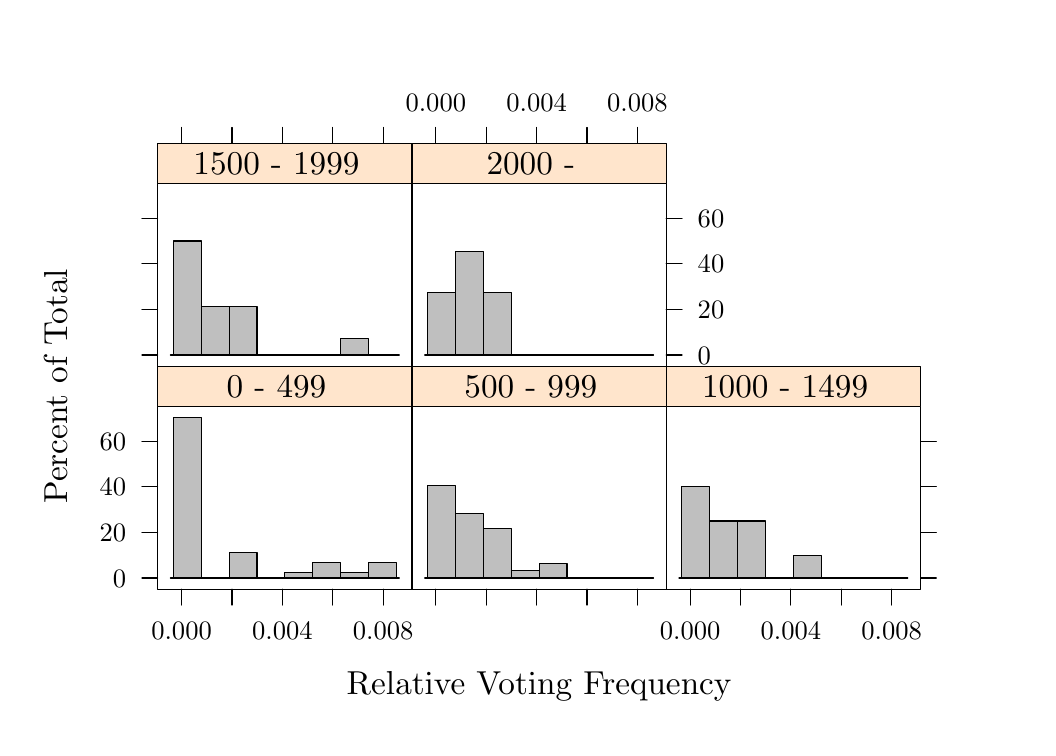
\begin{tikzpicture}[x=1pt,y=1pt]
\definecolor[named]{drawColor}{rgb}{0.00,0.00,0.00}
\definecolor[named]{fillColor}{rgb}{1.00,1.00,1.00}
\fill[color=fillColor,] (0,0) rectangle (361.35,252.94);
\begin{scope}
\path[clip] (  0.00,  0.00) rectangle (361.35,252.94);
\end{scope}
\begin{scope}
\path[clip] (  0.00,  0.00) rectangle (361.35,252.94);

\draw[fill opacity=0.00,draw opacity=0.00,] (  0.00,  0.00) rectangle (361.35,252.94);
\definecolor[named]{drawColor}{rgb}{0.00,0.00,0.00}

\node[color=drawColor,anchor=base,inner sep=0pt, outer sep=0pt, scale=  1.20] at (184.81, 12.04) {Relative Voting Frequency%
};
\end{scope}
\begin{scope}
\path[clip] (  0.00,  0.00) rectangle (361.35,252.94);
\definecolor[named]{drawColor}{rgb}{0.00,0.00,0.00}

\node[rotate= 90.00,color=drawColor,anchor=base,inner sep=0pt, outer sep=0pt, scale=  1.20] at ( 14.29,123.38) {Percent of Total%
};
\end{scope}
\begin{scope}
\path[clip] (  0.00,  0.00) rectangle (361.35,252.94);
\end{scope}
\begin{scope}
\path[clip] (  0.00,  0.00) rectangle (361.35,252.94);
\end{scope}
\begin{scope}
\path[clip] (  0.00,  0.00) rectangle (361.35,252.94);
\end{scope}
\begin{scope}
\path[clip] ( 46.98, 50.02) rectangle (138.86,116.15);
\end{scope}
\begin{scope}
\path[clip] (  0.00,  0.00) rectangle (361.35,252.94);
\end{scope}
\begin{scope}
\path[clip] (  0.00,  0.00) rectangle (361.35,252.94);
\end{scope}
\begin{scope}
\path[clip] (  0.00,  0.00) rectangle (361.35,252.94);
\end{scope}
\begin{scope}
\path[clip] (  0.00,  0.00) rectangle (361.35,252.94);
\definecolor[named]{drawColor}{rgb}{0.00,0.00,0.00}

\draw[color=drawColor,line cap=round,line join=round,fill opacity=0.00,] ( 46.98, 54.08) -- ( 41.29, 54.08);

\draw[color=drawColor,line cap=round,line join=round,fill opacity=0.00,] ( 46.98, 70.54) -- ( 41.29, 70.54);

\draw[color=drawColor,line cap=round,line join=round,fill opacity=0.00,] ( 46.98, 87.01) -- ( 41.29, 87.01);

\draw[color=drawColor,line cap=round,line join=round,fill opacity=0.00,] ( 46.98,103.48) -- ( 41.29,103.48);

\node[color=drawColor,anchor=base east,inner sep=0pt, outer sep=0pt, scale=  0.96] at ( 35.60, 50.77) {0%
};

\node[color=drawColor,anchor=base east,inner sep=0pt, outer sep=0pt, scale=  0.96] at ( 35.60, 67.24) {20%
};

\node[color=drawColor,anchor=base east,inner sep=0pt, outer sep=0pt, scale=  0.96] at ( 35.60, 83.71) {40%
};

\node[color=drawColor,anchor=base east,inner sep=0pt, outer sep=0pt, scale=  0.96] at ( 35.60,100.18) {60%
};
\end{scope}
\begin{scope}
\path[clip] (  0.00,  0.00) rectangle (361.35,252.94);
\end{scope}
\begin{scope}
\path[clip] (  0.00,  0.00) rectangle (361.35,252.94);
\definecolor[named]{drawColor}{rgb}{0.00,0.00,0.00}

\draw[color=drawColor,line cap=round,line join=round,fill opacity=0.00,] ( 55.61, 50.02) -- ( 55.61, 44.32);

\draw[color=drawColor,line cap=round,line join=round,fill opacity=0.00,] ( 73.82, 50.02) -- ( 73.82, 44.32);

\draw[color=drawColor,line cap=round,line join=round,fill opacity=0.00,] ( 92.03, 50.02) -- ( 92.03, 44.32);

\draw[color=drawColor,line cap=round,line join=round,fill opacity=0.00,] (110.24, 50.02) -- (110.24, 44.32);

\draw[color=drawColor,line cap=round,line join=round,fill opacity=0.00,] (128.45, 50.02) -- (128.45, 44.32);

\node[color=drawColor,anchor=base,inner sep=0pt, outer sep=0pt, scale=  0.96] at ( 55.61, 32.02) {0.000%
};

\node[color=drawColor,anchor=base,inner sep=0pt, outer sep=0pt, scale=  0.96] at ( 92.03, 32.02) {0.004%
};

\node[color=drawColor,anchor=base,inner sep=0pt, outer sep=0pt, scale=  0.96] at (128.45, 32.02) {0.008%
};
\end{scope}
\begin{scope}
\path[clip] (  0.00,  0.00) rectangle (361.35,252.94);
\end{scope}
\begin{scope}
\path[clip] ( 46.98, 50.02) rectangle (138.86,116.15);
\definecolor[named]{drawColor}{rgb}{0.00,0.00,0.00}

\draw[color=drawColor,line cap=round,line join=round,fill opacity=0.00,] ( 51.57, 54.08) --
	(134.27, 54.08);
\definecolor[named]{fillColor}{rgb}{0.75,0.75,0.75}

\draw[color=drawColor,line cap=round,line join=round,fill=fillColor,] ( 52.62, 54.08) rectangle ( 62.70,112.09);

\draw[color=drawColor,line cap=round,line join=round,fill=fillColor,] ( 62.70, 54.08) rectangle ( 72.77, 54.08);

\draw[color=drawColor,line cap=round,line join=round,fill=fillColor,] ( 72.77, 54.08) rectangle ( 82.85, 63.43);

\draw[color=drawColor,line cap=round,line join=round,fill=fillColor,] ( 82.85, 54.08) rectangle ( 92.92, 54.08);

\draw[color=drawColor,line cap=round,line join=round,fill=fillColor,] ( 92.92, 54.08) rectangle (103.00, 55.95);

\draw[color=drawColor,line cap=round,line join=round,fill=fillColor,] (103.00, 54.08) rectangle (113.07, 59.69);

\draw[color=drawColor,line cap=round,line join=round,fill=fillColor,] (113.07, 54.08) rectangle (123.15, 55.95);

\draw[color=drawColor,line cap=round,line join=round,fill=fillColor,] (123.15, 54.08) rectangle (133.22, 59.69);
\end{scope}
\begin{scope}
\path[clip] (  0.00,  0.00) rectangle (361.35,252.94);
\end{scope}
\begin{scope}
\path[clip] (  0.00,  0.00) rectangle (361.35,252.94);
\definecolor[named]{drawColor}{rgb}{0.00,0.00,0.00}

\draw[color=drawColor,line cap=round,line join=round,fill opacity=0.00,] ( 46.98, 50.02) rectangle (138.86,116.15);
\end{scope}
\begin{scope}
\path[clip] (  0.00,  0.00) rectangle (361.35,252.94);
\end{scope}
\begin{scope}
\path[clip] (  0.00,  0.00) rectangle (361.35,252.94);
\end{scope}
\begin{scope}
\path[clip] ( 46.98,116.15) rectangle (138.86,130.60);
\definecolor[named]{drawColor}{rgb}{1.00,0.90,0.80}
\definecolor[named]{fillColor}{rgb}{1.00,0.90,0.80}

\draw[color=drawColor,line cap=round,line join=round,fill=fillColor,] ( 46.98,116.15) rectangle (138.86,130.60);
\definecolor[named]{drawColor}{rgb}{0.00,0.00,0.00}

\node[color=drawColor,anchor=base ,inner sep=0pt, outer sep=0pt, scale=  1.20] at ( 89.92,119.25) {0 - 499%
};
\end{scope}
\begin{scope}
\path[clip] (  0.00,  0.00) rectangle (361.35,252.94);
\end{scope}
\begin{scope}
\path[clip] (  0.00,  0.00) rectangle (361.35,252.94);
\definecolor[named]{drawColor}{rgb}{0.00,0.00,0.00}

\draw[color=drawColor,line cap=round,line join=round,fill opacity=0.00,] ( 46.98,116.15) rectangle (138.86,130.60);
\end{scope}
\begin{scope}
\path[clip] (  0.00,  0.00) rectangle (361.35,252.94);
\end{scope}
\begin{scope}
\path[clip] (  0.00,  0.00) rectangle (361.35,252.94);
\end{scope}
\begin{scope}
\path[clip] (138.86, 50.02) rectangle (230.75,116.15);
\end{scope}
\begin{scope}
\path[clip] (  0.00,  0.00) rectangle (361.35,252.94);
\end{scope}
\begin{scope}
\path[clip] (  0.00,  0.00) rectangle (361.35,252.94);
\end{scope}
\begin{scope}
\path[clip] (  0.00,  0.00) rectangle (361.35,252.94);
\end{scope}
\begin{scope}
\path[clip] (  0.00,  0.00) rectangle (361.35,252.94);
\end{scope}
\begin{scope}
\path[clip] (  0.00,  0.00) rectangle (361.35,252.94);
\end{scope}
\begin{scope}
\path[clip] (  0.00,  0.00) rectangle (361.35,252.94);
\definecolor[named]{drawColor}{rgb}{0.00,0.00,0.00}

\draw[color=drawColor,line cap=round,line join=round,fill opacity=0.00,] (147.49, 50.02) -- (147.49, 44.32);

\draw[color=drawColor,line cap=round,line join=round,fill opacity=0.00,] (165.70, 50.02) -- (165.70, 44.32);

\draw[color=drawColor,line cap=round,line join=round,fill opacity=0.00,] (183.91, 50.02) -- (183.91, 44.32);

\draw[color=drawColor,line cap=round,line join=round,fill opacity=0.00,] (202.12, 50.02) -- (202.12, 44.32);

\draw[color=drawColor,line cap=round,line join=round,fill opacity=0.00,] (220.33, 50.02) -- (220.33, 44.32);
\end{scope}
\begin{scope}
\path[clip] (  0.00,  0.00) rectangle (361.35,252.94);
\end{scope}
\begin{scope}
\path[clip] (138.86, 50.02) rectangle (230.75,116.15);
\definecolor[named]{drawColor}{rgb}{0.00,0.00,0.00}

\draw[color=drawColor,line cap=round,line join=round,fill opacity=0.00,] (143.46, 54.08) --
	(226.16, 54.08);
\definecolor[named]{fillColor}{rgb}{0.75,0.75,0.75}

\draw[color=drawColor,line cap=round,line join=round,fill=fillColor,] (144.51, 54.08) rectangle (154.58, 87.53);

\draw[color=drawColor,line cap=round,line join=round,fill=fillColor,] (154.58, 54.08) rectangle (164.66, 77.24);

\draw[color=drawColor,line cap=round,line join=round,fill=fillColor,] (164.66, 54.08) rectangle (174.73, 72.09);

\draw[color=drawColor,line cap=round,line join=round,fill=fillColor,] (174.73, 54.08) rectangle (184.81, 56.65);

\draw[color=drawColor,line cap=round,line join=round,fill=fillColor,] (184.81, 54.08) rectangle (194.88, 59.22);

\draw[color=drawColor,line cap=round,line join=round,fill=fillColor,] (194.88, 54.08) rectangle (204.96, 54.08);

\draw[color=drawColor,line cap=round,line join=round,fill=fillColor,] (204.96, 54.08) rectangle (215.03, 54.08);

\draw[color=drawColor,line cap=round,line join=round,fill=fillColor,] (215.03, 54.08) rectangle (225.11, 54.08);
\end{scope}
\begin{scope}
\path[clip] (  0.00,  0.00) rectangle (361.35,252.94);
\end{scope}
\begin{scope}
\path[clip] (  0.00,  0.00) rectangle (361.35,252.94);
\definecolor[named]{drawColor}{rgb}{0.00,0.00,0.00}

\draw[color=drawColor,line cap=round,line join=round,fill opacity=0.00,] (138.86, 50.02) rectangle (230.75,116.15);
\end{scope}
\begin{scope}
\path[clip] (  0.00,  0.00) rectangle (361.35,252.94);
\end{scope}
\begin{scope}
\path[clip] (  0.00,  0.00) rectangle (361.35,252.94);
\end{scope}
\begin{scope}
\path[clip] (138.86,116.15) rectangle (230.75,130.60);
\definecolor[named]{drawColor}{rgb}{1.00,0.90,0.80}
\definecolor[named]{fillColor}{rgb}{1.00,0.90,0.80}

\draw[color=drawColor,line cap=round,line join=round,fill=fillColor,] (138.86,116.15) rectangle (230.75,130.60);
\definecolor[named]{drawColor}{rgb}{0.00,0.00,0.00}

\node[color=drawColor,anchor=base ,inner sep=0pt, outer sep=0pt, scale=  1.20] at (181.81,119.25) {500 - 999%
};
\end{scope}
\begin{scope}
\path[clip] (  0.00,  0.00) rectangle (361.35,252.94);
\end{scope}
\begin{scope}
\path[clip] (  0.00,  0.00) rectangle (361.35,252.94);
\definecolor[named]{drawColor}{rgb}{0.00,0.00,0.00}

\draw[color=drawColor,line cap=round,line join=round,fill opacity=0.00,] (138.86,116.15) rectangle (230.75,130.60);
\end{scope}
\begin{scope}
\path[clip] (  0.00,  0.00) rectangle (361.35,252.94);
\end{scope}
\begin{scope}
\path[clip] (  0.00,  0.00) rectangle (361.35,252.94);
\end{scope}
\begin{scope}
\path[clip] (230.75, 50.02) rectangle (322.64,116.15);
\end{scope}
\begin{scope}
\path[clip] (  0.00,  0.00) rectangle (361.35,252.94);
\end{scope}
\begin{scope}
\path[clip] (  0.00,  0.00) rectangle (361.35,252.94);
\end{scope}
\begin{scope}
\path[clip] (  0.00,  0.00) rectangle (361.35,252.94);
\end{scope}
\begin{scope}
\path[clip] (  0.00,  0.00) rectangle (361.35,252.94);
\end{scope}
\begin{scope}
\path[clip] (  0.00,  0.00) rectangle (361.35,252.94);
\end{scope}
\begin{scope}
\path[clip] (  0.00,  0.00) rectangle (361.35,252.94);
\definecolor[named]{drawColor}{rgb}{0.00,0.00,0.00}

\draw[color=drawColor,line cap=round,line join=round,fill opacity=0.00,] (239.38, 50.02) -- (239.38, 44.32);

\draw[color=drawColor,line cap=round,line join=round,fill opacity=0.00,] (257.59, 50.02) -- (257.59, 44.32);

\draw[color=drawColor,line cap=round,line join=round,fill opacity=0.00,] (275.80, 50.02) -- (275.80, 44.32);

\draw[color=drawColor,line cap=round,line join=round,fill opacity=0.00,] (294.01, 50.02) -- (294.01, 44.32);

\draw[color=drawColor,line cap=round,line join=round,fill opacity=0.00,] (312.22, 50.02) -- (312.22, 44.32);

\node[color=drawColor,anchor=base,inner sep=0pt, outer sep=0pt, scale=  0.96] at (239.38, 32.02) {0.000%
};

\node[color=drawColor,anchor=base,inner sep=0pt, outer sep=0pt, scale=  0.96] at (275.80, 32.02) {0.004%
};

\node[color=drawColor,anchor=base,inner sep=0pt, outer sep=0pt, scale=  0.96] at (312.22, 32.02) {0.008%
};

\draw[color=drawColor,line cap=round,line join=round,fill opacity=0.00,] (322.64, 54.08) -- (328.33, 54.08);

\draw[color=drawColor,line cap=round,line join=round,fill opacity=0.00,] (322.64, 70.54) -- (328.33, 70.54);

\draw[color=drawColor,line cap=round,line join=round,fill opacity=0.00,] (322.64, 87.01) -- (328.33, 87.01);

\draw[color=drawColor,line cap=round,line join=round,fill opacity=0.00,] (322.64,103.48) -- (328.33,103.48);
\end{scope}
\begin{scope}
\path[clip] (  0.00,  0.00) rectangle (361.35,252.94);
\end{scope}
\begin{scope}
\path[clip] (230.75, 50.02) rectangle (322.64,116.15);
\definecolor[named]{drawColor}{rgb}{0.00,0.00,0.00}

\draw[color=drawColor,line cap=round,line join=round,fill opacity=0.00,] (235.34, 54.08) --
	(318.04, 54.08);
\definecolor[named]{fillColor}{rgb}{0.75,0.75,0.75}

\draw[color=drawColor,line cap=round,line join=round,fill=fillColor,] (236.39, 54.08) rectangle (246.47, 87.01);

\draw[color=drawColor,line cap=round,line join=round,fill=fillColor,] (246.47, 54.08) rectangle (256.54, 74.66);

\draw[color=drawColor,line cap=round,line join=round,fill=fillColor,] (256.54, 54.08) rectangle (266.62, 74.66);

\draw[color=drawColor,line cap=round,line join=round,fill=fillColor,] (266.62, 54.08) rectangle (276.69, 54.08);

\draw[color=drawColor,line cap=round,line join=round,fill=fillColor,] (276.69, 54.08) rectangle (286.77, 62.31);

\draw[color=drawColor,line cap=round,line join=round,fill=fillColor,] (286.77, 54.08) rectangle (296.84, 54.08);

\draw[color=drawColor,line cap=round,line join=round,fill=fillColor,] (296.84, 54.08) rectangle (306.92, 54.08);

\draw[color=drawColor,line cap=round,line join=round,fill=fillColor,] (306.92, 54.08) rectangle (316.99, 54.08);
\end{scope}
\begin{scope}
\path[clip] (  0.00,  0.00) rectangle (361.35,252.94);
\end{scope}
\begin{scope}
\path[clip] (  0.00,  0.00) rectangle (361.35,252.94);
\definecolor[named]{drawColor}{rgb}{0.00,0.00,0.00}

\draw[color=drawColor,line cap=round,line join=round,fill opacity=0.00,] (230.75, 50.02) rectangle (322.64,116.15);
\end{scope}
\begin{scope}
\path[clip] (  0.00,  0.00) rectangle (361.35,252.94);
\end{scope}
\begin{scope}
\path[clip] (  0.00,  0.00) rectangle (361.35,252.94);
\end{scope}
\begin{scope}
\path[clip] (230.75,116.15) rectangle (322.64,130.60);
\definecolor[named]{drawColor}{rgb}{1.00,0.90,0.80}
\definecolor[named]{fillColor}{rgb}{1.00,0.90,0.80}

\draw[color=drawColor,line cap=round,line join=round,fill=fillColor,] (230.75,116.15) rectangle (322.64,130.60);
\definecolor[named]{drawColor}{rgb}{0.00,0.00,0.00}

\node[color=drawColor,anchor=base ,inner sep=0pt, outer sep=0pt, scale=  1.20] at (273.69,119.25) {1000 - 1499%
};
\end{scope}
\begin{scope}
\path[clip] (  0.00,  0.00) rectangle (361.35,252.94);
\end{scope}
\begin{scope}
\path[clip] (  0.00,  0.00) rectangle (361.35,252.94);
\definecolor[named]{drawColor}{rgb}{0.00,0.00,0.00}

\draw[color=drawColor,line cap=round,line join=round,fill opacity=0.00,] (230.75,116.15) rectangle (322.64,130.60);
\end{scope}
\begin{scope}
\path[clip] (  0.00,  0.00) rectangle (361.35,252.94);
\end{scope}
\begin{scope}
\path[clip] (  0.00,  0.00) rectangle (361.35,252.94);
\end{scope}
\begin{scope}
\path[clip] ( 46.98,130.60) rectangle (138.86,196.74);
\end{scope}
\begin{scope}
\path[clip] (  0.00,  0.00) rectangle (361.35,252.94);
\end{scope}
\begin{scope}
\path[clip] (  0.00,  0.00) rectangle (361.35,252.94);
\definecolor[named]{drawColor}{rgb}{0.00,0.00,0.00}

\draw[color=drawColor,line cap=round,line join=round,fill opacity=0.00,] ( 55.61,211.19) -- ( 55.61,216.88);

\draw[color=drawColor,line cap=round,line join=round,fill opacity=0.00,] ( 73.82,211.19) -- ( 73.82,216.88);

\draw[color=drawColor,line cap=round,line join=round,fill opacity=0.00,] ( 92.03,211.19) -- ( 92.03,216.88);

\draw[color=drawColor,line cap=round,line join=round,fill opacity=0.00,] (110.24,211.19) -- (110.24,216.88);

\draw[color=drawColor,line cap=round,line join=round,fill opacity=0.00,] (128.45,211.19) -- (128.45,216.88);
\end{scope}
\begin{scope}
\path[clip] (  0.00,  0.00) rectangle (361.35,252.94);
\end{scope}
\begin{scope}
\path[clip] (  0.00,  0.00) rectangle (361.35,252.94);
\definecolor[named]{drawColor}{rgb}{0.00,0.00,0.00}

\draw[color=drawColor,line cap=round,line join=round,fill opacity=0.00,] ( 46.98,134.67) -- ( 41.29,134.67);

\draw[color=drawColor,line cap=round,line join=round,fill opacity=0.00,] ( 46.98,151.13) -- ( 41.29,151.13);

\draw[color=drawColor,line cap=round,line join=round,fill opacity=0.00,] ( 46.98,167.60) -- ( 41.29,167.60);

\draw[color=drawColor,line cap=round,line join=round,fill opacity=0.00,] ( 46.98,184.07) -- ( 41.29,184.07);
\end{scope}
\begin{scope}
\path[clip] (  0.00,  0.00) rectangle (361.35,252.94);
\end{scope}
\begin{scope}
\path[clip] (  0.00,  0.00) rectangle (361.35,252.94);
\end{scope}
\begin{scope}
\path[clip] (  0.00,  0.00) rectangle (361.35,252.94);
\end{scope}
\begin{scope}
\path[clip] ( 46.98,130.60) rectangle (138.86,196.74);
\definecolor[named]{drawColor}{rgb}{0.00,0.00,0.00}

\draw[color=drawColor,line cap=round,line join=round,fill opacity=0.00,] ( 51.57,134.67) --
	(134.27,134.67);
\definecolor[named]{fillColor}{rgb}{0.75,0.75,0.75}

\draw[color=drawColor,line cap=round,line join=round,fill=fillColor,] ( 52.62,134.67) rectangle ( 62.70,175.84);

\draw[color=drawColor,line cap=round,line join=round,fill=fillColor,] ( 62.70,134.67) rectangle ( 72.77,152.31);

\draw[color=drawColor,line cap=round,line join=round,fill=fillColor,] ( 72.77,134.67) rectangle ( 82.85,152.31);

\draw[color=drawColor,line cap=round,line join=round,fill=fillColor,] ( 82.85,134.67) rectangle ( 92.92,134.67);

\draw[color=drawColor,line cap=round,line join=round,fill=fillColor,] ( 92.92,134.67) rectangle (103.00,134.67);

\draw[color=drawColor,line cap=round,line join=round,fill=fillColor,] (103.00,134.67) rectangle (113.07,134.67);

\draw[color=drawColor,line cap=round,line join=round,fill=fillColor,] (113.07,134.67) rectangle (123.15,140.55);

\draw[color=drawColor,line cap=round,line join=round,fill=fillColor,] (123.15,134.67) rectangle (133.22,134.67);
\end{scope}
\begin{scope}
\path[clip] (  0.00,  0.00) rectangle (361.35,252.94);
\end{scope}
\begin{scope}
\path[clip] (  0.00,  0.00) rectangle (361.35,252.94);
\definecolor[named]{drawColor}{rgb}{0.00,0.00,0.00}

\draw[color=drawColor,line cap=round,line join=round,fill opacity=0.00,] ( 46.98,130.60) rectangle (138.86,196.74);
\end{scope}
\begin{scope}
\path[clip] (  0.00,  0.00) rectangle (361.35,252.94);
\end{scope}
\begin{scope}
\path[clip] (  0.00,  0.00) rectangle (361.35,252.94);
\end{scope}
\begin{scope}
\path[clip] ( 46.98,196.74) rectangle (138.86,211.19);
\definecolor[named]{drawColor}{rgb}{1.00,0.90,0.80}
\definecolor[named]{fillColor}{rgb}{1.00,0.90,0.80}

\draw[color=drawColor,line cap=round,line join=round,fill=fillColor,] ( 46.98,196.74) rectangle (138.86,211.19);
\definecolor[named]{drawColor}{rgb}{0.00,0.00,0.00}

\node[color=drawColor,anchor=base ,inner sep=0pt, outer sep=0pt, scale=  1.20] at ( 89.92,199.83) {1500 - 1999%
};
\end{scope}
\begin{scope}
\path[clip] (  0.00,  0.00) rectangle (361.35,252.94);
\end{scope}
\begin{scope}
\path[clip] (  0.00,  0.00) rectangle (361.35,252.94);
\definecolor[named]{drawColor}{rgb}{0.00,0.00,0.00}

\draw[color=drawColor,line cap=round,line join=round,fill opacity=0.00,] ( 46.98,196.74) rectangle (138.86,211.19);
\end{scope}
\begin{scope}
\path[clip] (  0.00,  0.00) rectangle (361.35,252.94);
\end{scope}
\begin{scope}
\path[clip] (  0.00,  0.00) rectangle (361.35,252.94);
\end{scope}
\begin{scope}
\path[clip] (138.86,130.60) rectangle (230.75,196.74);
\end{scope}
\begin{scope}
\path[clip] (  0.00,  0.00) rectangle (361.35,252.94);
\end{scope}
\begin{scope}
\path[clip] (  0.00,  0.00) rectangle (361.35,252.94);
\definecolor[named]{drawColor}{rgb}{0.00,0.00,0.00}

\draw[color=drawColor,line cap=round,line join=round,fill opacity=0.00,] (147.49,211.19) -- (147.49,216.88);

\draw[color=drawColor,line cap=round,line join=round,fill opacity=0.00,] (165.70,211.19) -- (165.70,216.88);

\draw[color=drawColor,line cap=round,line join=round,fill opacity=0.00,] (183.91,211.19) -- (183.91,216.88);

\draw[color=drawColor,line cap=round,line join=round,fill opacity=0.00,] (202.12,211.19) -- (202.12,216.88);

\draw[color=drawColor,line cap=round,line join=round,fill opacity=0.00,] (220.33,211.19) -- (220.33,216.88);

\node[color=drawColor,anchor=base,inner sep=0pt, outer sep=0pt, scale=  0.96] at (147.49,222.58) {0.000%
};

\node[color=drawColor,anchor=base,inner sep=0pt, outer sep=0pt, scale=  0.96] at (183.91,222.58) {0.004%
};

\node[color=drawColor,anchor=base,inner sep=0pt, outer sep=0pt, scale=  0.96] at (220.33,222.58) {0.008%
};
\end{scope}
\begin{scope}
\path[clip] (  0.00,  0.00) rectangle (361.35,252.94);
\end{scope}
\begin{scope}
\path[clip] (  0.00,  0.00) rectangle (361.35,252.94);
\end{scope}
\begin{scope}
\path[clip] (  0.00,  0.00) rectangle (361.35,252.94);
\end{scope}
\begin{scope}
\path[clip] (  0.00,  0.00) rectangle (361.35,252.94);
\definecolor[named]{drawColor}{rgb}{0.00,0.00,0.00}

\draw[color=drawColor,line cap=round,line join=round,fill opacity=0.00,] (230.75,134.67) -- (236.44,134.67);

\draw[color=drawColor,line cap=round,line join=round,fill opacity=0.00,] (230.75,151.13) -- (236.44,151.13);

\draw[color=drawColor,line cap=round,line join=round,fill opacity=0.00,] (230.75,167.60) -- (236.44,167.60);

\draw[color=drawColor,line cap=round,line join=round,fill opacity=0.00,] (230.75,184.07) -- (236.44,184.07);

\node[color=drawColor,anchor=base west,inner sep=0pt, outer sep=0pt, scale=  0.96] at (242.13,131.36) {0%
};

\node[color=drawColor,anchor=base west,inner sep=0pt, outer sep=0pt, scale=  0.96] at (242.13,147.83) {20%
};

\node[color=drawColor,anchor=base west,inner sep=0pt, outer sep=0pt, scale=  0.96] at (242.13,164.30) {40%
};

\node[color=drawColor,anchor=base west,inner sep=0pt, outer sep=0pt, scale=  0.96] at (242.13,180.76) {60%
};
\end{scope}
\begin{scope}
\path[clip] (  0.00,  0.00) rectangle (361.35,252.94);
\end{scope}
\begin{scope}
\path[clip] (138.86,130.60) rectangle (230.75,196.74);
\definecolor[named]{drawColor}{rgb}{0.00,0.00,0.00}

\draw[color=drawColor,line cap=round,line join=round,fill opacity=0.00,] (143.46,134.67) --
	(226.16,134.67);
\definecolor[named]{fillColor}{rgb}{0.75,0.75,0.75}

\draw[color=drawColor,line cap=round,line join=round,fill=fillColor,] (144.51,134.67) rectangle (154.58,157.12);

\draw[color=drawColor,line cap=round,line join=round,fill=fillColor,] (154.58,134.67) rectangle (164.66,172.09);

\draw[color=drawColor,line cap=round,line join=round,fill=fillColor,] (164.66,134.67) rectangle (174.73,157.12);

\draw[color=drawColor,line cap=round,line join=round,fill=fillColor,] (174.73,134.67) rectangle (184.81,134.67);

\draw[color=drawColor,line cap=round,line join=round,fill=fillColor,] (184.81,134.67) rectangle (194.88,134.67);

\draw[color=drawColor,line cap=round,line join=round,fill=fillColor,] (194.88,134.67) rectangle (204.96,134.67);

\draw[color=drawColor,line cap=round,line join=round,fill=fillColor,] (204.96,134.67) rectangle (215.03,134.67);

\draw[color=drawColor,line cap=round,line join=round,fill=fillColor,] (215.03,134.67) rectangle (225.11,134.67);
\end{scope}
\begin{scope}
\path[clip] (  0.00,  0.00) rectangle (361.35,252.94);
\end{scope}
\begin{scope}
\path[clip] (  0.00,  0.00) rectangle (361.35,252.94);
\definecolor[named]{drawColor}{rgb}{0.00,0.00,0.00}

\draw[color=drawColor,line cap=round,line join=round,fill opacity=0.00,] (138.86,130.60) rectangle (230.75,196.74);
\end{scope}
\begin{scope}
\path[clip] (  0.00,  0.00) rectangle (361.35,252.94);
\end{scope}
\begin{scope}
\path[clip] (  0.00,  0.00) rectangle (361.35,252.94);
\end{scope}
\begin{scope}
\path[clip] (138.86,196.74) rectangle (230.75,211.19);
\definecolor[named]{drawColor}{rgb}{1.00,0.90,0.80}
\definecolor[named]{fillColor}{rgb}{1.00,0.90,0.80}

\draw[color=drawColor,line cap=round,line join=round,fill=fillColor,] (138.86,196.74) rectangle (230.75,211.19);
\definecolor[named]{drawColor}{rgb}{0.00,0.00,0.00}

\node[color=drawColor,anchor=base ,inner sep=0pt, outer sep=0pt, scale=  1.20] at (181.81,199.83) {2000 -%
};
\end{scope}
\begin{scope}
\path[clip] (  0.00,  0.00) rectangle (361.35,252.94);
\end{scope}
\begin{scope}
\path[clip] (  0.00,  0.00) rectangle (361.35,252.94);
\definecolor[named]{drawColor}{rgb}{0.00,0.00,0.00}

\draw[color=drawColor,line cap=round,line join=round,fill opacity=0.00,] (138.86,196.74) rectangle (230.75,211.19);
\end{scope}
\begin{scope}
\path[clip] (  0.00,  0.00) rectangle (361.35,252.94);
\end{scope}
\begin{scope}
\path[clip] (  0.00,  0.00) rectangle (361.35,252.94);
\end{scope}
\begin{scope}
\path[clip] (  0.00,  0.00) rectangle (361.35,252.94);
\end{scope}
\begin{scope}
\path[clip] (  0.00,  0.00) rectangle (361.35,252.94);
\end{scope}
\end{tikzpicture}
}}\quad
\scalebox{.6}{\subfloat[][Yes Votes with a Dissenting Statement]{% Created by tikzDevice version 0.6.1 on 2011-07-24 21:12:33
% !TEX encoding = UTF-8 Unicode
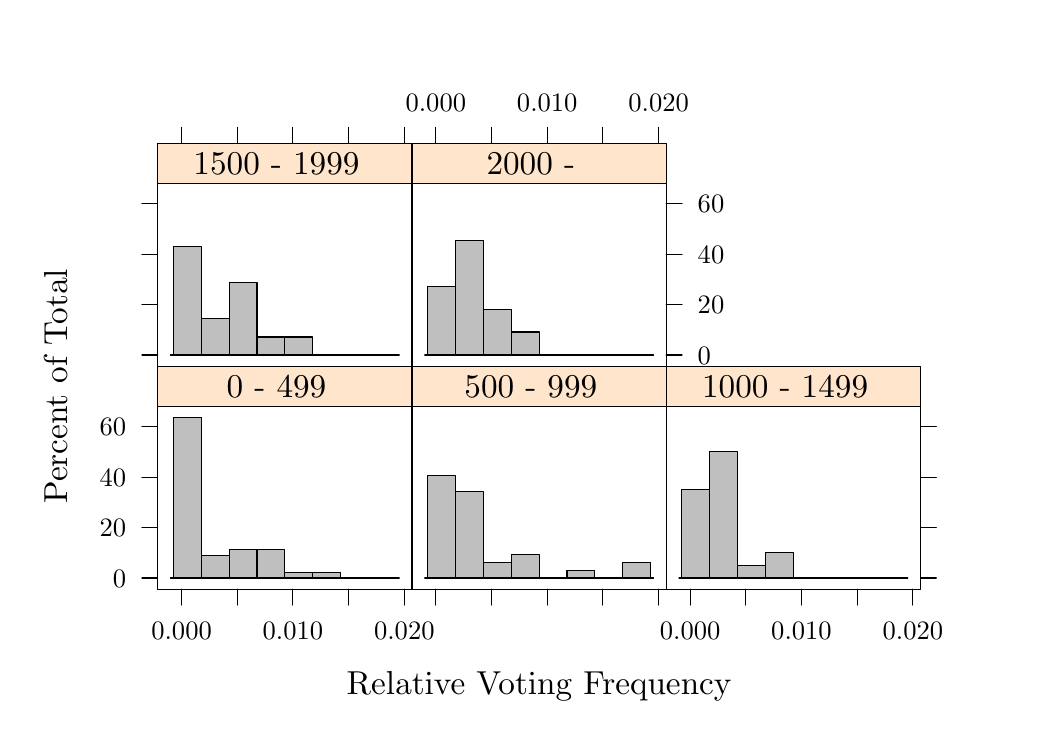
\begin{tikzpicture}[x=1pt,y=1pt]
\definecolor[named]{drawColor}{rgb}{0.00,0.00,0.00}
\definecolor[named]{fillColor}{rgb}{1.00,1.00,1.00}
\fill[color=fillColor,] (0,0) rectangle (361.35,252.94);
\begin{scope}
\path[clip] (  0.00,  0.00) rectangle (361.35,252.94);
\end{scope}
\begin{scope}
\path[clip] (  0.00,  0.00) rectangle (361.35,252.94);

\draw[fill opacity=0.00,draw opacity=0.00,] (  0.00,  0.00) rectangle (361.35,252.94);
\definecolor[named]{drawColor}{rgb}{0.00,0.00,0.00}

\node[color=drawColor,anchor=base,inner sep=0pt, outer sep=0pt, scale=  1.20] at (184.81, 12.04) {Relative Voting Frequency%
};
\end{scope}
\begin{scope}
\path[clip] (  0.00,  0.00) rectangle (361.35,252.94);
\definecolor[named]{drawColor}{rgb}{0.00,0.00,0.00}

\node[rotate= 90.00,color=drawColor,anchor=base,inner sep=0pt, outer sep=0pt, scale=  1.20] at ( 14.29,123.38) {Percent of Total%
};
\end{scope}
\begin{scope}
\path[clip] (  0.00,  0.00) rectangle (361.35,252.94);
\end{scope}
\begin{scope}
\path[clip] (  0.00,  0.00) rectangle (361.35,252.94);
\end{scope}
\begin{scope}
\path[clip] (  0.00,  0.00) rectangle (361.35,252.94);
\end{scope}
\begin{scope}
\path[clip] ( 46.98, 50.02) rectangle (138.86,116.15);
\end{scope}
\begin{scope}
\path[clip] (  0.00,  0.00) rectangle (361.35,252.94);
\end{scope}
\begin{scope}
\path[clip] (  0.00,  0.00) rectangle (361.35,252.94);
\end{scope}
\begin{scope}
\path[clip] (  0.00,  0.00) rectangle (361.35,252.94);
\end{scope}
\begin{scope}
\path[clip] (  0.00,  0.00) rectangle (361.35,252.94);
\definecolor[named]{drawColor}{rgb}{0.00,0.00,0.00}

\draw[color=drawColor,line cap=round,line join=round,fill opacity=0.00,] ( 46.98, 54.08) -- ( 41.29, 54.08);

\draw[color=drawColor,line cap=round,line join=round,fill opacity=0.00,] ( 46.98, 72.31) -- ( 41.29, 72.31);

\draw[color=drawColor,line cap=round,line join=round,fill opacity=0.00,] ( 46.98, 90.54) -- ( 41.29, 90.54);

\draw[color=drawColor,line cap=round,line join=round,fill opacity=0.00,] ( 46.98,108.77) -- ( 41.29,108.77);

\node[color=drawColor,anchor=base east,inner sep=0pt, outer sep=0pt, scale=  0.96] at ( 35.60, 50.77) {0%
};

\node[color=drawColor,anchor=base east,inner sep=0pt, outer sep=0pt, scale=  0.96] at ( 35.60, 69.00) {20%
};

\node[color=drawColor,anchor=base east,inner sep=0pt, outer sep=0pt, scale=  0.96] at ( 35.60, 87.24) {40%
};

\node[color=drawColor,anchor=base east,inner sep=0pt, outer sep=0pt, scale=  0.96] at ( 35.60,105.47) {60%
};
\end{scope}
\begin{scope}
\path[clip] (  0.00,  0.00) rectangle (361.35,252.94);
\end{scope}
\begin{scope}
\path[clip] (  0.00,  0.00) rectangle (361.35,252.94);
\definecolor[named]{drawColor}{rgb}{0.00,0.00,0.00}

\draw[color=drawColor,line cap=round,line join=round,fill opacity=0.00,] ( 55.61, 50.02) -- ( 55.61, 44.32);

\draw[color=drawColor,line cap=round,line join=round,fill opacity=0.00,] ( 75.73, 50.02) -- ( 75.73, 44.32);

\draw[color=drawColor,line cap=round,line join=round,fill opacity=0.00,] ( 95.85, 50.02) -- ( 95.85, 44.32);

\draw[color=drawColor,line cap=round,line join=round,fill opacity=0.00,] (115.98, 50.02) -- (115.98, 44.32);

\draw[color=drawColor,line cap=round,line join=round,fill opacity=0.00,] (136.10, 50.02) -- (136.10, 44.32);

\node[color=drawColor,anchor=base,inner sep=0pt, outer sep=0pt, scale=  0.96] at ( 55.61, 32.02) {0.000%
};

\node[color=drawColor,anchor=base,inner sep=0pt, outer sep=0pt, scale=  0.96] at ( 95.85, 32.02) {0.010%
};

\node[color=drawColor,anchor=base,inner sep=0pt, outer sep=0pt, scale=  0.96] at (136.10, 32.02) {0.020%
};
\end{scope}
\begin{scope}
\path[clip] (  0.00,  0.00) rectangle (361.35,252.94);
\end{scope}
\begin{scope}
\path[clip] ( 46.98, 50.02) rectangle (138.86,116.15);
\definecolor[named]{drawColor}{rgb}{0.00,0.00,0.00}

\draw[color=drawColor,line cap=round,line join=round,fill opacity=0.00,] ( 51.57, 54.08) --
	(134.27, 54.08);
\definecolor[named]{fillColor}{rgb}{0.75,0.75,0.75}

\draw[color=drawColor,line cap=round,line join=round,fill=fillColor,] ( 52.62, 54.08) rectangle ( 62.70,112.09);

\draw[color=drawColor,line cap=round,line join=round,fill=fillColor,] ( 62.70, 54.08) rectangle ( 72.77, 62.36);

\draw[color=drawColor,line cap=round,line join=round,fill=fillColor,] ( 72.77, 54.08) rectangle ( 82.85, 64.44);

\draw[color=drawColor,line cap=round,line join=round,fill=fillColor,] ( 82.85, 54.08) rectangle ( 92.92, 64.44);

\draw[color=drawColor,line cap=round,line join=round,fill=fillColor,] ( 92.92, 54.08) rectangle (103.00, 56.15);

\draw[color=drawColor,line cap=round,line join=round,fill=fillColor,] (103.00, 54.08) rectangle (113.07, 56.15);

\draw[color=drawColor,line cap=round,line join=round,fill=fillColor,] (113.07, 54.08) rectangle (123.15, 54.08);

\draw[color=drawColor,line cap=round,line join=round,fill=fillColor,] (123.15, 54.08) rectangle (133.22, 54.08);
\end{scope}
\begin{scope}
\path[clip] (  0.00,  0.00) rectangle (361.35,252.94);
\end{scope}
\begin{scope}
\path[clip] (  0.00,  0.00) rectangle (361.35,252.94);
\definecolor[named]{drawColor}{rgb}{0.00,0.00,0.00}

\draw[color=drawColor,line cap=round,line join=round,fill opacity=0.00,] ( 46.98, 50.02) rectangle (138.86,116.15);
\end{scope}
\begin{scope}
\path[clip] (  0.00,  0.00) rectangle (361.35,252.94);
\end{scope}
\begin{scope}
\path[clip] (  0.00,  0.00) rectangle (361.35,252.94);
\end{scope}
\begin{scope}
\path[clip] ( 46.98,116.15) rectangle (138.86,130.60);
\definecolor[named]{drawColor}{rgb}{1.00,0.90,0.80}
\definecolor[named]{fillColor}{rgb}{1.00,0.90,0.80}

\draw[color=drawColor,line cap=round,line join=round,fill=fillColor,] ( 46.98,116.15) rectangle (138.86,130.60);
\definecolor[named]{drawColor}{rgb}{0.00,0.00,0.00}

\node[color=drawColor,anchor=base ,inner sep=0pt, outer sep=0pt, scale=  1.20] at ( 89.92,119.25) {0 - 499%
};
\end{scope}
\begin{scope}
\path[clip] (  0.00,  0.00) rectangle (361.35,252.94);
\end{scope}
\begin{scope}
\path[clip] (  0.00,  0.00) rectangle (361.35,252.94);
\definecolor[named]{drawColor}{rgb}{0.00,0.00,0.00}

\draw[color=drawColor,line cap=round,line join=round,fill opacity=0.00,] ( 46.98,116.15) rectangle (138.86,130.60);
\end{scope}
\begin{scope}
\path[clip] (  0.00,  0.00) rectangle (361.35,252.94);
\end{scope}
\begin{scope}
\path[clip] (  0.00,  0.00) rectangle (361.35,252.94);
\end{scope}
\begin{scope}
\path[clip] (138.86, 50.02) rectangle (230.75,116.15);
\end{scope}
\begin{scope}
\path[clip] (  0.00,  0.00) rectangle (361.35,252.94);
\end{scope}
\begin{scope}
\path[clip] (  0.00,  0.00) rectangle (361.35,252.94);
\end{scope}
\begin{scope}
\path[clip] (  0.00,  0.00) rectangle (361.35,252.94);
\end{scope}
\begin{scope}
\path[clip] (  0.00,  0.00) rectangle (361.35,252.94);
\end{scope}
\begin{scope}
\path[clip] (  0.00,  0.00) rectangle (361.35,252.94);
\end{scope}
\begin{scope}
\path[clip] (  0.00,  0.00) rectangle (361.35,252.94);
\definecolor[named]{drawColor}{rgb}{0.00,0.00,0.00}

\draw[color=drawColor,line cap=round,line join=round,fill opacity=0.00,] (147.49, 50.02) -- (147.49, 44.32);

\draw[color=drawColor,line cap=round,line join=round,fill opacity=0.00,] (167.62, 50.02) -- (167.62, 44.32);

\draw[color=drawColor,line cap=round,line join=round,fill opacity=0.00,] (187.74, 50.02) -- (187.74, 44.32);

\draw[color=drawColor,line cap=round,line join=round,fill opacity=0.00,] (207.86, 50.02) -- (207.86, 44.32);

\draw[color=drawColor,line cap=round,line join=round,fill opacity=0.00,] (227.99, 50.02) -- (227.99, 44.32);
\end{scope}
\begin{scope}
\path[clip] (  0.00,  0.00) rectangle (361.35,252.94);
\end{scope}
\begin{scope}
\path[clip] (138.86, 50.02) rectangle (230.75,116.15);
\definecolor[named]{drawColor}{rgb}{0.00,0.00,0.00}

\draw[color=drawColor,line cap=round,line join=round,fill opacity=0.00,] (143.46, 54.08) --
	(226.16, 54.08);
\definecolor[named]{fillColor}{rgb}{0.75,0.75,0.75}

\draw[color=drawColor,line cap=round,line join=round,fill=fillColor,] (144.51, 54.08) rectangle (154.58, 91.11);

\draw[color=drawColor,line cap=round,line join=round,fill=fillColor,] (154.58, 54.08) rectangle (164.66, 85.41);

\draw[color=drawColor,line cap=round,line join=round,fill=fillColor,] (164.66, 54.08) rectangle (174.73, 59.77);

\draw[color=drawColor,line cap=round,line join=round,fill=fillColor,] (174.73, 54.08) rectangle (184.81, 62.62);

\draw[color=drawColor,line cap=round,line join=round,fill=fillColor,] (184.81, 54.08) rectangle (194.88, 54.08);

\draw[color=drawColor,line cap=round,line join=round,fill=fillColor,] (194.88, 54.08) rectangle (204.96, 56.93);

\draw[color=drawColor,line cap=round,line join=round,fill=fillColor,] (204.96, 54.08) rectangle (215.03, 54.08);

\draw[color=drawColor,line cap=round,line join=round,fill=fillColor,] (215.03, 54.08) rectangle (225.11, 59.77);
\end{scope}
\begin{scope}
\path[clip] (  0.00,  0.00) rectangle (361.35,252.94);
\end{scope}
\begin{scope}
\path[clip] (  0.00,  0.00) rectangle (361.35,252.94);
\definecolor[named]{drawColor}{rgb}{0.00,0.00,0.00}

\draw[color=drawColor,line cap=round,line join=round,fill opacity=0.00,] (138.86, 50.02) rectangle (230.75,116.15);
\end{scope}
\begin{scope}
\path[clip] (  0.00,  0.00) rectangle (361.35,252.94);
\end{scope}
\begin{scope}
\path[clip] (  0.00,  0.00) rectangle (361.35,252.94);
\end{scope}
\begin{scope}
\path[clip] (138.86,116.15) rectangle (230.75,130.60);
\definecolor[named]{drawColor}{rgb}{1.00,0.90,0.80}
\definecolor[named]{fillColor}{rgb}{1.00,0.90,0.80}

\draw[color=drawColor,line cap=round,line join=round,fill=fillColor,] (138.86,116.15) rectangle (230.75,130.60);
\definecolor[named]{drawColor}{rgb}{0.00,0.00,0.00}

\node[color=drawColor,anchor=base ,inner sep=0pt, outer sep=0pt, scale=  1.20] at (181.81,119.25) {500 - 999%
};
\end{scope}
\begin{scope}
\path[clip] (  0.00,  0.00) rectangle (361.35,252.94);
\end{scope}
\begin{scope}
\path[clip] (  0.00,  0.00) rectangle (361.35,252.94);
\definecolor[named]{drawColor}{rgb}{0.00,0.00,0.00}

\draw[color=drawColor,line cap=round,line join=round,fill opacity=0.00,] (138.86,116.15) rectangle (230.75,130.60);
\end{scope}
\begin{scope}
\path[clip] (  0.00,  0.00) rectangle (361.35,252.94);
\end{scope}
\begin{scope}
\path[clip] (  0.00,  0.00) rectangle (361.35,252.94);
\end{scope}
\begin{scope}
\path[clip] (230.75, 50.02) rectangle (322.64,116.15);
\end{scope}
\begin{scope}
\path[clip] (  0.00,  0.00) rectangle (361.35,252.94);
\end{scope}
\begin{scope}
\path[clip] (  0.00,  0.00) rectangle (361.35,252.94);
\end{scope}
\begin{scope}
\path[clip] (  0.00,  0.00) rectangle (361.35,252.94);
\end{scope}
\begin{scope}
\path[clip] (  0.00,  0.00) rectangle (361.35,252.94);
\end{scope}
\begin{scope}
\path[clip] (  0.00,  0.00) rectangle (361.35,252.94);
\end{scope}
\begin{scope}
\path[clip] (  0.00,  0.00) rectangle (361.35,252.94);
\definecolor[named]{drawColor}{rgb}{0.00,0.00,0.00}

\draw[color=drawColor,line cap=round,line join=round,fill opacity=0.00,] (239.38, 50.02) -- (239.38, 44.32);

\draw[color=drawColor,line cap=round,line join=round,fill opacity=0.00,] (259.50, 50.02) -- (259.50, 44.32);

\draw[color=drawColor,line cap=round,line join=round,fill opacity=0.00,] (279.62, 50.02) -- (279.62, 44.32);

\draw[color=drawColor,line cap=round,line join=round,fill opacity=0.00,] (299.75, 50.02) -- (299.75, 44.32);

\draw[color=drawColor,line cap=round,line join=round,fill opacity=0.00,] (319.87, 50.02) -- (319.87, 44.32);

\node[color=drawColor,anchor=base,inner sep=0pt, outer sep=0pt, scale=  0.96] at (239.38, 32.02) {0.000%
};

\node[color=drawColor,anchor=base,inner sep=0pt, outer sep=0pt, scale=  0.96] at (279.62, 32.02) {0.010%
};

\node[color=drawColor,anchor=base,inner sep=0pt, outer sep=0pt, scale=  0.96] at (319.87, 32.02) {0.020%
};

\draw[color=drawColor,line cap=round,line join=round,fill opacity=0.00,] (322.64, 54.08) -- (328.33, 54.08);

\draw[color=drawColor,line cap=round,line join=round,fill opacity=0.00,] (322.64, 72.31) -- (328.33, 72.31);

\draw[color=drawColor,line cap=round,line join=round,fill opacity=0.00,] (322.64, 90.54) -- (328.33, 90.54);

\draw[color=drawColor,line cap=round,line join=round,fill opacity=0.00,] (322.64,108.77) -- (328.33,108.77);
\end{scope}
\begin{scope}
\path[clip] (  0.00,  0.00) rectangle (361.35,252.94);
\end{scope}
\begin{scope}
\path[clip] (230.75, 50.02) rectangle (322.64,116.15);
\definecolor[named]{drawColor}{rgb}{0.00,0.00,0.00}

\draw[color=drawColor,line cap=round,line join=round,fill opacity=0.00,] (235.34, 54.08) --
	(318.04, 54.08);
\definecolor[named]{fillColor}{rgb}{0.75,0.75,0.75}

\draw[color=drawColor,line cap=round,line join=round,fill=fillColor,] (236.39, 54.08) rectangle (246.47, 85.98);

\draw[color=drawColor,line cap=round,line join=round,fill=fillColor,] (246.47, 54.08) rectangle (256.54, 99.66);

\draw[color=drawColor,line cap=round,line join=round,fill=fillColor,] (256.54, 54.08) rectangle (266.62, 58.63);

\draw[color=drawColor,line cap=round,line join=round,fill=fillColor,] (266.62, 54.08) rectangle (276.69, 63.19);

\draw[color=drawColor,line cap=round,line join=round,fill=fillColor,] (276.69, 54.08) rectangle (286.77, 54.08);

\draw[color=drawColor,line cap=round,line join=round,fill=fillColor,] (286.77, 54.08) rectangle (296.84, 54.08);

\draw[color=drawColor,line cap=round,line join=round,fill=fillColor,] (296.84, 54.08) rectangle (306.92, 54.08);

\draw[color=drawColor,line cap=round,line join=round,fill=fillColor,] (306.92, 54.08) rectangle (316.99, 54.08);
\end{scope}
\begin{scope}
\path[clip] (  0.00,  0.00) rectangle (361.35,252.94);
\end{scope}
\begin{scope}
\path[clip] (  0.00,  0.00) rectangle (361.35,252.94);
\definecolor[named]{drawColor}{rgb}{0.00,0.00,0.00}

\draw[color=drawColor,line cap=round,line join=round,fill opacity=0.00,] (230.75, 50.02) rectangle (322.64,116.15);
\end{scope}
\begin{scope}
\path[clip] (  0.00,  0.00) rectangle (361.35,252.94);
\end{scope}
\begin{scope}
\path[clip] (  0.00,  0.00) rectangle (361.35,252.94);
\end{scope}
\begin{scope}
\path[clip] (230.75,116.15) rectangle (322.64,130.60);
\definecolor[named]{drawColor}{rgb}{1.00,0.90,0.80}
\definecolor[named]{fillColor}{rgb}{1.00,0.90,0.80}

\draw[color=drawColor,line cap=round,line join=round,fill=fillColor,] (230.75,116.15) rectangle (322.64,130.60);
\definecolor[named]{drawColor}{rgb}{0.00,0.00,0.00}

\node[color=drawColor,anchor=base ,inner sep=0pt, outer sep=0pt, scale=  1.20] at (273.69,119.25) {1000 - 1499%
};
\end{scope}
\begin{scope}
\path[clip] (  0.00,  0.00) rectangle (361.35,252.94);
\end{scope}
\begin{scope}
\path[clip] (  0.00,  0.00) rectangle (361.35,252.94);
\definecolor[named]{drawColor}{rgb}{0.00,0.00,0.00}

\draw[color=drawColor,line cap=round,line join=round,fill opacity=0.00,] (230.75,116.15) rectangle (322.64,130.60);
\end{scope}
\begin{scope}
\path[clip] (  0.00,  0.00) rectangle (361.35,252.94);
\end{scope}
\begin{scope}
\path[clip] (  0.00,  0.00) rectangle (361.35,252.94);
\end{scope}
\begin{scope}
\path[clip] ( 46.98,130.60) rectangle (138.86,196.74);
\end{scope}
\begin{scope}
\path[clip] (  0.00,  0.00) rectangle (361.35,252.94);
\end{scope}
\begin{scope}
\path[clip] (  0.00,  0.00) rectangle (361.35,252.94);
\definecolor[named]{drawColor}{rgb}{0.00,0.00,0.00}

\draw[color=drawColor,line cap=round,line join=round,fill opacity=0.00,] ( 55.61,211.19) -- ( 55.61,216.88);

\draw[color=drawColor,line cap=round,line join=round,fill opacity=0.00,] ( 75.73,211.19) -- ( 75.73,216.88);

\draw[color=drawColor,line cap=round,line join=round,fill opacity=0.00,] ( 95.85,211.19) -- ( 95.85,216.88);

\draw[color=drawColor,line cap=round,line join=round,fill opacity=0.00,] (115.98,211.19) -- (115.98,216.88);

\draw[color=drawColor,line cap=round,line join=round,fill opacity=0.00,] (136.10,211.19) -- (136.10,216.88);
\end{scope}
\begin{scope}
\path[clip] (  0.00,  0.00) rectangle (361.35,252.94);
\end{scope}
\begin{scope}
\path[clip] (  0.00,  0.00) rectangle (361.35,252.94);
\definecolor[named]{drawColor}{rgb}{0.00,0.00,0.00}

\draw[color=drawColor,line cap=round,line join=round,fill opacity=0.00,] ( 46.98,134.67) -- ( 41.29,134.67);

\draw[color=drawColor,line cap=round,line join=round,fill opacity=0.00,] ( 46.98,152.90) -- ( 41.29,152.90);

\draw[color=drawColor,line cap=round,line join=round,fill opacity=0.00,] ( 46.98,171.13) -- ( 41.29,171.13);

\draw[color=drawColor,line cap=round,line join=round,fill opacity=0.00,] ( 46.98,189.36) -- ( 41.29,189.36);
\end{scope}
\begin{scope}
\path[clip] (  0.00,  0.00) rectangle (361.35,252.94);
\end{scope}
\begin{scope}
\path[clip] (  0.00,  0.00) rectangle (361.35,252.94);
\end{scope}
\begin{scope}
\path[clip] (  0.00,  0.00) rectangle (361.35,252.94);
\end{scope}
\begin{scope}
\path[clip] ( 46.98,130.60) rectangle (138.86,196.74);
\definecolor[named]{drawColor}{rgb}{0.00,0.00,0.00}

\draw[color=drawColor,line cap=round,line join=round,fill opacity=0.00,] ( 51.57,134.67) --
	(134.27,134.67);
\definecolor[named]{fillColor}{rgb}{0.75,0.75,0.75}

\draw[color=drawColor,line cap=round,line join=round,fill=fillColor,] ( 52.62,134.67) rectangle ( 62.70,173.74);

\draw[color=drawColor,line cap=round,line join=round,fill=fillColor,] ( 62.70,134.67) rectangle ( 72.77,147.69);

\draw[color=drawColor,line cap=round,line join=round,fill=fillColor,] ( 72.77,134.67) rectangle ( 82.85,160.71);

\draw[color=drawColor,line cap=round,line join=round,fill=fillColor,] ( 82.85,134.67) rectangle ( 92.92,141.18);

\draw[color=drawColor,line cap=round,line join=round,fill=fillColor,] ( 92.92,134.67) rectangle (103.00,141.18);

\draw[color=drawColor,line cap=round,line join=round,fill=fillColor,] (103.00,134.67) rectangle (113.07,134.67);

\draw[color=drawColor,line cap=round,line join=round,fill=fillColor,] (113.07,134.67) rectangle (123.15,134.67);

\draw[color=drawColor,line cap=round,line join=round,fill=fillColor,] (123.15,134.67) rectangle (133.22,134.67);
\end{scope}
\begin{scope}
\path[clip] (  0.00,  0.00) rectangle (361.35,252.94);
\end{scope}
\begin{scope}
\path[clip] (  0.00,  0.00) rectangle (361.35,252.94);
\definecolor[named]{drawColor}{rgb}{0.00,0.00,0.00}

\draw[color=drawColor,line cap=round,line join=round,fill opacity=0.00,] ( 46.98,130.60) rectangle (138.86,196.74);
\end{scope}
\begin{scope}
\path[clip] (  0.00,  0.00) rectangle (361.35,252.94);
\end{scope}
\begin{scope}
\path[clip] (  0.00,  0.00) rectangle (361.35,252.94);
\end{scope}
\begin{scope}
\path[clip] ( 46.98,196.74) rectangle (138.86,211.19);
\definecolor[named]{drawColor}{rgb}{1.00,0.90,0.80}
\definecolor[named]{fillColor}{rgb}{1.00,0.90,0.80}

\draw[color=drawColor,line cap=round,line join=round,fill=fillColor,] ( 46.98,196.74) rectangle (138.86,211.19);
\definecolor[named]{drawColor}{rgb}{0.00,0.00,0.00}

\node[color=drawColor,anchor=base ,inner sep=0pt, outer sep=0pt, scale=  1.20] at ( 89.92,199.83) {1500 - 1999%
};
\end{scope}
\begin{scope}
\path[clip] (  0.00,  0.00) rectangle (361.35,252.94);
\end{scope}
\begin{scope}
\path[clip] (  0.00,  0.00) rectangle (361.35,252.94);
\definecolor[named]{drawColor}{rgb}{0.00,0.00,0.00}

\draw[color=drawColor,line cap=round,line join=round,fill opacity=0.00,] ( 46.98,196.74) rectangle (138.86,211.19);
\end{scope}
\begin{scope}
\path[clip] (  0.00,  0.00) rectangle (361.35,252.94);
\end{scope}
\begin{scope}
\path[clip] (  0.00,  0.00) rectangle (361.35,252.94);
\end{scope}
\begin{scope}
\path[clip] (138.86,130.60) rectangle (230.75,196.74);
\end{scope}
\begin{scope}
\path[clip] (  0.00,  0.00) rectangle (361.35,252.94);
\end{scope}
\begin{scope}
\path[clip] (  0.00,  0.00) rectangle (361.35,252.94);
\definecolor[named]{drawColor}{rgb}{0.00,0.00,0.00}

\draw[color=drawColor,line cap=round,line join=round,fill opacity=0.00,] (147.49,211.19) -- (147.49,216.88);

\draw[color=drawColor,line cap=round,line join=round,fill opacity=0.00,] (167.62,211.19) -- (167.62,216.88);

\draw[color=drawColor,line cap=round,line join=round,fill opacity=0.00,] (187.74,211.19) -- (187.74,216.88);

\draw[color=drawColor,line cap=round,line join=round,fill opacity=0.00,] (207.86,211.19) -- (207.86,216.88);

\draw[color=drawColor,line cap=round,line join=round,fill opacity=0.00,] (227.99,211.19) -- (227.99,216.88);

\node[color=drawColor,anchor=base,inner sep=0pt, outer sep=0pt, scale=  0.96] at (147.49,222.58) {0.000%
};

\node[color=drawColor,anchor=base,inner sep=0pt, outer sep=0pt, scale=  0.96] at (187.74,222.58) {0.010%
};

\node[color=drawColor,anchor=base,inner sep=0pt, outer sep=0pt, scale=  0.96] at (227.99,222.58) {0.020%
};
\end{scope}
\begin{scope}
\path[clip] (  0.00,  0.00) rectangle (361.35,252.94);
\end{scope}
\begin{scope}
\path[clip] (  0.00,  0.00) rectangle (361.35,252.94);
\end{scope}
\begin{scope}
\path[clip] (  0.00,  0.00) rectangle (361.35,252.94);
\end{scope}
\begin{scope}
\path[clip] (  0.00,  0.00) rectangle (361.35,252.94);
\definecolor[named]{drawColor}{rgb}{0.00,0.00,0.00}

\draw[color=drawColor,line cap=round,line join=round,fill opacity=0.00,] (230.75,134.67) -- (236.44,134.67);

\draw[color=drawColor,line cap=round,line join=round,fill opacity=0.00,] (230.75,152.90) -- (236.44,152.90);

\draw[color=drawColor,line cap=round,line join=round,fill opacity=0.00,] (230.75,171.13) -- (236.44,171.13);

\draw[color=drawColor,line cap=round,line join=round,fill opacity=0.00,] (230.75,189.36) -- (236.44,189.36);

\node[color=drawColor,anchor=base west,inner sep=0pt, outer sep=0pt, scale=  0.96] at (242.13,131.36) {0%
};

\node[color=drawColor,anchor=base west,inner sep=0pt, outer sep=0pt, scale=  0.96] at (242.13,149.59) {20%
};

\node[color=drawColor,anchor=base west,inner sep=0pt, outer sep=0pt, scale=  0.96] at (242.13,167.83) {40%
};

\node[color=drawColor,anchor=base west,inner sep=0pt, outer sep=0pt, scale=  0.96] at (242.13,186.06) {60%
};
\end{scope}
\begin{scope}
\path[clip] (  0.00,  0.00) rectangle (361.35,252.94);
\end{scope}
\begin{scope}
\path[clip] (138.86,130.60) rectangle (230.75,196.74);
\definecolor[named]{drawColor}{rgb}{0.00,0.00,0.00}

\draw[color=drawColor,line cap=round,line join=round,fill opacity=0.00,] (143.46,134.67) --
	(226.16,134.67);
\definecolor[named]{fillColor}{rgb}{0.75,0.75,0.75}

\draw[color=drawColor,line cap=round,line join=round,fill=fillColor,] (144.51,134.67) rectangle (154.58,159.53);

\draw[color=drawColor,line cap=round,line join=round,fill=fillColor,] (154.58,134.67) rectangle (164.66,176.10);

\draw[color=drawColor,line cap=round,line join=round,fill=fillColor,] (164.66,134.67) rectangle (174.73,151.24);

\draw[color=drawColor,line cap=round,line join=round,fill=fillColor,] (174.73,134.67) rectangle (184.81,142.95);

\draw[color=drawColor,line cap=round,line join=round,fill=fillColor,] (184.81,134.67) rectangle (194.88,134.67);

\draw[color=drawColor,line cap=round,line join=round,fill=fillColor,] (194.88,134.67) rectangle (204.96,134.67);

\draw[color=drawColor,line cap=round,line join=round,fill=fillColor,] (204.96,134.67) rectangle (215.03,134.67);

\draw[color=drawColor,line cap=round,line join=round,fill=fillColor,] (215.03,134.67) rectangle (225.11,134.67);
\end{scope}
\begin{scope}
\path[clip] (  0.00,  0.00) rectangle (361.35,252.94);
\end{scope}
\begin{scope}
\path[clip] (  0.00,  0.00) rectangle (361.35,252.94);
\definecolor[named]{drawColor}{rgb}{0.00,0.00,0.00}

\draw[color=drawColor,line cap=round,line join=round,fill opacity=0.00,] (138.86,130.60) rectangle (230.75,196.74);
\end{scope}
\begin{scope}
\path[clip] (  0.00,  0.00) rectangle (361.35,252.94);
\end{scope}
\begin{scope}
\path[clip] (  0.00,  0.00) rectangle (361.35,252.94);
\end{scope}
\begin{scope}
\path[clip] (138.86,196.74) rectangle (230.75,211.19);
\definecolor[named]{drawColor}{rgb}{1.00,0.90,0.80}
\definecolor[named]{fillColor}{rgb}{1.00,0.90,0.80}

\draw[color=drawColor,line cap=round,line join=round,fill=fillColor,] (138.86,196.74) rectangle (230.75,211.19);
\definecolor[named]{drawColor}{rgb}{0.00,0.00,0.00}

\node[color=drawColor,anchor=base ,inner sep=0pt, outer sep=0pt, scale=  1.20] at (181.81,199.83) {2000 -%
};
\end{scope}
\begin{scope}
\path[clip] (  0.00,  0.00) rectangle (361.35,252.94);
\end{scope}
\begin{scope}
\path[clip] (  0.00,  0.00) rectangle (361.35,252.94);
\definecolor[named]{drawColor}{rgb}{0.00,0.00,0.00}

\draw[color=drawColor,line cap=round,line join=round,fill opacity=0.00,] (138.86,196.74) rectangle (230.75,211.19);
\end{scope}
\begin{scope}
\path[clip] (  0.00,  0.00) rectangle (361.35,252.94);
\end{scope}
\begin{scope}
\path[clip] (  0.00,  0.00) rectangle (361.35,252.94);
\end{scope}
\begin{scope}
\path[clip] (  0.00,  0.00) rectangle (361.35,252.94);
\end{scope}
\begin{scope}
\path[clip] (  0.00,  0.00) rectangle (361.35,252.94);
\end{scope}
\end{tikzpicture}
}}\quad
\caption{The plots show the conditional distribution of relative voting frequencies within each time category.}
\label{fig:histogram}
\end{figure}

The important aspect to notice in Figure \ref{fig:histogram} is that for the no votes, conditioning on meeting frequency does not change the distribution in any significant way. The choice to cast a no vote is independent of the time spend in the Council. This corroborates the thesis that no votes are signaling devices aimed at domestic audiences, as the interest of domestic audiences in the dossiers coming from the Commission are independent of time. For abstentions and yes votes with a dissenting statement we see that the number of governments that has not cast a vote in this category decrease as time passes, lending partial corroborating evidence for hypothesis three.




\section{Inferential Analysis}
In order to further test the hypotheses we turn to statistical modeling. The dependent variable is the vote choice of the individual government, since it is difficult to rank the variable a multinomial logistic choice model is appropriate. The multinomial model is a generalization of the logistic regression model, basically dividing the choice categories into pairs, and estimating a logit model for each pair. The model equations can be written as:

\begin{equation}
  \label{eq:3}
  Pr(y_i = k) = \frac{exp(x_i\beta_k)}{\sum_{j = 1}^j exp(x_i \beta_j)}
\end{equation}

Where for the $i$th individual $y_i$ is the observed outcome, $x_i$ is a vector of explanatory variables, and $\beta_k$ is a vector of parameters associated with the single choice, and $\beta_j$ is a vector of parameters associated with the alternative choices. Equation \ref{eq:3} nicely illustrate that coefficients in the multinomial model are relative to each other, i.e. unlike in most regression models we cannot make any absolute statements about effect, but only make statements about effect sizes relative to different choices. Furthermore the coefficients, bar the last statement, can be interpreted much like any standard logit model. 


The multinomial model is suitable first and foremost as they do not make any assumptions about the ordinality of a variable, furthermore they do not make any assumption about normality, linearity and homogeneity of variance of the independent variables. Thus these models represent a very flexible modeling framework when dealing with choice categories. However there are two crucial assumptions made in these models which must be justified. The first assumption is commonly labelled independence of irrelevant alternatives (IIA). This assumes that the results from the analysis would not change if we threw in another choice category which would clearly be irrelevant to the problem being modeled. The classic example is the study of modes of transport. If subjects has to make a choice between taking the bus, ride a bike or taking the car to work, then the results from such an analysis should not change if we added two bus categories, one with red busses and one with blue busses. Since the color coding of busses should be irrelevant we would expect the subjects to randomly choose between the two busses. In the Council data we already have an exhaustive list of choice options, and it is not cleat which alternatives that could be added, hence the IIA assumption is not judged to be a problem with the data at hand. The second, more serious, assumption is that we have enough data to cover the different cells created by the tabulation of the dependent and independent variables. Because the model uses multiple equations and a maximum likelihood estimation technique there are high demands on sample size. A rule of thumb is that the case to variable ratio should at least 20:1, in the analysis conducted here the maximum number of variables used are 100, since we have a sample size of 13527 this gives a ratio of ca. 135:1. Hence sample size is not a problem for the analysis. 

Hypothesis one states that the choice to vote no is governed by domestic pressure. It is very difficult to get a measure of domestic pressure for each government on each dossier, hence the testing of this hypothesis presents some difficulties. It is well known that some member states have national interests that are independent of the government in office. Spain, for instance, commands the largest fishing fleet in the EU, and the fishing industry employs a large share of the Spanish workforce. Thus Spain is under pressure to ensure optimal conditions for the fishing industry, including making sure that the vessels are allowed to catch as many fish as possible. Likewise Germany is a heavily export oriented economy, hence with regards to the internal market they are likely to resist any attempt to restrict the free movement of goods. The considerations laid forward here implies that there can be country and policy specific domestic constituencies that can pressure governments. In order to account for this we have included a separate analysis for the major policy areas and in each model member state dummies are included. If a member state dummy is significant we can attribute this to member state specific effects. Controlling for other relevant variables, any effect is likely due to domestic political concerns.  

With regards to hypothesis two a continuous direct measure of outlier status is calculated by the following formula:

\begin{equation}
  \label{eq:4}
  O_i = (a_{pi} - \bar{x}_{p})^2
\end{equation}

Where $O_i$ is the outlier status of government $i$, $a_{pi}$ is the left-right position of government i, and $\bar{x}_{p}$ is the mean government position in the Council. This variable should be highly significant in determining whether a government will abstain or not on a given dossier. 

Finally, for hypothesis three we use a measure of meeting activity within the Council configuration under which a dossier was treated. The measure is a count of all the meetings in a given year for a given Council configuration, and thus only varies on a  yearly basis. One potential issue with this variable is that it assumes the same degree of socialization at the beginning and end of a year, thus any governments entering the Council will be associated with a degree of socialization that might not be appropriate. This is, however, mitigated by the fact that the permanent representatives in the Council usually survive the governments, and thus they can be counted on to pass on their knowledge of Council negotiations to new governments. 

\subsection{Control Variables}

There are a number of possible confounding variables that must be included in the analysis to properly estimate the independent effect of our main variables. The usual suspect are power, the presidency and budget considerations, below each variable will be considered in detail. 

Many scholars argue that more powerful member states use their power to influence the final outcome. Power is a difficult concept to measure. Most studies on the Council distinguish between powerful actors along three closely related dimensions, namely number of votes in the Council, size of a member state and GDP (either per capita or absolute). Number of votes and population size are closely, although not linearly, related. Indeed number of votes in the Council is a function of the population of a given member state. There is a large literature on a priori power of member states utilizing voting power indexes. It is well known that often the raw number of votes do not translate directly into influence \citep{Gelman2003a}. However in the Council the shapley-shubik index provides the same ranking of member states as the raw number of votes. Measures of GDP have been used in a number of studies as a measure of economic power \citep{DeSoysa1997}. However the use of GDP per capita in a EU context poses significant problems. In the EU there are a num- ber of smaller very affluent states (Luxembourg is the classic example). These states all score very high on this measure, even surpassing the UK, Germany and France, whereas in absolute terms they are dwarfed by the big member states. That big member states enjoy more latitude due to their dominance in terms of population and GDP at the sum- mit level has been documented by \citet{Tallberg2008} In a series of elite interviews with heads of state and senior negotiators he find a general consensus among summit participants that population and economic size is directly related to the influence a member state can wield. how- ever at the Council level there does not seem to be much of an effect of GDP and decision making in the Council (Heisenberg 2005). In the literature power is hypothesized to have two effects. First, influential states will be able to move outcomes closer to their ideal, and thus we should expect states witha high GDP and votes in the Council to vote yes more often than their counterparts. Second, influential states will be more willing to make their differences with the Council majority public, and thus they will tend to vote no or abstain more often than small member states (Mattila, 2004). These two effects are not mutually exclusive, instead they refer to the situation where large member states might find themselves being preference outliers, and hence not able to move outcome close enough to their ideal point. In these situations it is hypothesized that large member states,having a high degree of influence, and being involved on more issues than smaller member states will express their dissatisfaction. The underlying mechanism is one where powerful member states (in terms of size and GDP) will have more ressources available when negotiating in Bruxelles. This allows them to be active on more dossiers, thus increasing the chance they might find themselves in a minority position. Smaller member states will focus their ressources on key dossiers. This implies that there is an interaction effect between preferences and power. Large member states who are also preference outliers will vote no more often than small member states, regardless of whether the smaller member state is a preference outlier or not. Hence it is important to control for the potential power of a given government. To make the variables easier to interpret in the analysis the raw vote count of each member state is used in the analysis as a control for the potential power of governments.

The Council of the EU has unique institutional feature in the rotating presidency. The presidency follows a six month rotation, and it is custom that each presidency identifies key issues that will be the focus for the next period. The original intention with the rotating presidency was to distribute authority within the EU, in order to avoid concen- trating agenda setting powers on any group or member state (Kollman, 2003, p. 54). The presidency has recently been studied in quite some detail. From a qualitative perspective Tallberg (2004, 2001, 2003) has provided a series of in depth case studies detailing how member states can use the presidency to influence negotiations. Tallberg locates the source of the influence the presidency can wield in its position as an “honest” broker. By virtue of this position the presidency gains insight into the positions of the conflicting parties. It is not unusual in Council negotiations that the presidency has private “confessionals” with member states that prevent a decision to be reached (Tallberg, 2004, p. 1004). The presidency also has a praxis of touring the capitals of member states in order to collect information on difficult dossiers. All Council sessions are managed by the Presidency, which can con- trol the agenda and style of session (i.e. with or without senior civil servants). FInally the presidency has the prerogative of proposing a compromise text which, if agreed upon in the Council, will supplant the text from the Commission. These attributes of the presidency gives the government currently in the seat considerable scope for influencing the outcomes of negotiations. However there are limits as the presidency is build on an informal praxis, and has very few formal powers. Thus if a presidency blatantly misuses the information gained in the confessionals, the member state risks not only that the other Council members will not accept any compromise proposals put forth, but also undermining the foundation on which the presidency is build. How- ever, that member states do use the presidency for their own gain has been amply documented in literature. During the end negotiations of the transparency regulation in 2001, the Swedish presidency where actively promoting their own agenda, but:

\begin{quote}
``Swedish activities during the transparency negotiations brought considerable criticism. The constraining force of the norm is still evidenced by the efforts made to keep the appearance of being impartial''
\flushright{- \citealt[264]{BjurulfElgstrom2004}}
\end{quote}

From a quantitative perspective the presidency has also attracted considerable attention. Schalk et al. (2007) use the DEU data to test whether the member state holding the Council presidency is able to influence the outcomes. They find that there is only an effect of the presidency in the final stages of negotiation, where as government that precede when a dossier is introduced do not have any significant influence. This finding has been replicated by Warntjen (2008) in a regression analysis controlling for process, voting rule, and type of legal act (using the same data). He finds that the effect of holding the presidency during the final stages of a negotiation shifts the outcome closer to the member states preferences by a factor between 2 and 4, depending on the model, in comparison to not having the presidency.
The evidence speaks for an effect of the presidency in the Council, although one should keep in mind that the DEU data used only contain dossiers from 2000-2001. Thus it is not clear if the presidency effect is consistent over time or not. However the effect on voting behavior is straight forward. If the council presidency has to give the impression of being impartial, and the presidency is able to influence the outcome considerably, we should expect to see governments holding the presidency exhibit a markedly non-conflictual voting behavior. 

A popular distinction between member states in the literature on the Council is between net contributors to the budget and net beneficiaries from the budget. A common argument is that member states that contribute more than they gain from the EU budget will be more inclined to demand to keep expenses to redistributive programs as low as possible. In the words of Zimmer et al.:

\begin{quote}
``To a certain extent, the wealthy member states are willing to buy of the consent of the poorer nations by means of sub- sidies.''
\flushright{- \citealt[407]{ZimmerSchneiderDobbins2005}}
\end{quote}


One proposed mechanism behind this ``buy-out'' of poor member states, is that typically the more wealthy member states are also export oriented. In order to have a functioning internal market the poorer member states must allow the import of goods from other member states, but they stand to gain less from the opening up of the other markets. In order to compensate for this perceived injustice more of the EU budget is allocated to these states, with the implicit understanding that they will not block the decision making process in the Council \citep{Hix2005}. The implication is that member states that receive large amounts of funding through the different funds of the EU, should be less conflictual in Council negotiations, as long as their subsides remain untouched. Given that subsides are mainly given in the agricultural and regional policy areas, we should expect net beneficiaries to oppose any change in these areas, whereas they will act consensual in other policy areas. In this sense it is important to control for whether a member state is a net-beneficiary or not, and introduce a dummy for agricultural and regional policy areas. 

It is also important to account for any procedural aspects that might confound the results, hence the voting rule and legislative instrument are included as control variables. The independent variables are measured on two levels, namely the dossier level and the member state government level. The member state government is the lowest level in the data, and are nested with the dossier level, such that for each dossier we have recorded between 15 and 27 votes that are attributed to governments from the member states. Table \ref{tab:variables} show the independent variables along with the source and descriptive statistics. 

\begin{table}[ht]
  \centering
   \resizebox{\textwidth}{!}{
  \begin{tabular}{l p{5cm} l c c} \toprule
    Variable & Description & Source &  Mean/Mode/Median & Standard Deviation \\ \midrule
    Left-Right & The position of each government on a 0 to 10 scale, where 0 is most left and 10 is most right. & \citet{DoringMannow2010} & 5.33 & 1.42 \\ 
    Votes & The number of votes a given member state has at its disposal. & Council & 5 & 6.98 \\
    Presidency & Categorical variable coding for which member state holds the Presidency at the time of voting. & Council & - & - \\
    Net Beneficiary & The net amount of contributions to the EU mins the net amount of funds received from the EU. & EU Budget Reports & -0.16 & 178.84 \\
Meeting Frequency & The number of sessions per year for the different Council configurations & Council  & 8 & 4.64 \\
Voting Rule & A dummy variable coding 0 for unanimity and 1 for QMV. & Council & - & - \\
Type of Legal Act & A categorical variable coding whether a dossier was a directive, regulation or decision & PreLex  & - & - \\
   \bottomrule
  \end{tabular}
  }
  \caption{Independent Variables}
  \label{tab:variables}
\end{table}

\subsection{Analysis}

Due to a high degree of collienarity between some variables and the presence of many empty cells in the data set, the analysis will focus on three policy areas in which the data is sufficient. These policy areas are agriculture and fisheries, competition and employment and consumer affairs. Two variables in the data set are highly collinear, namely the raw vote count and the member state dummy variable. Two models were estimated for each policy area, one with the raw vote count of member states, and one with member state dummies.  There were no substantial difference between the two models, and in order to account for member state specific effects, the results from the model with member state dummies are reported in this section. Due to the complexity of the models, in this section only the predicted probabilities from the models are presented. 

In figures \ref{fig:devEmplCons} and \ref{fig:meetEmplCons} the predicted probabilities from the employment and consumer affairs model are depicted. For each choice category the other variables have been held constant at their mean/median values. The effect of the variables allowed to vary has been plotted for each member state. The reference category has been defined as voting no, hence the probabilities plotted are all relative to the probability of voting no. 

\begin{figure}[htp]
  \centering
  \scalebox{.7}{
    % Created by tikzDevice version 0.6.1 on 2011-08-02 12:45:09
% !TEX encoding = UTF-8 Unicode
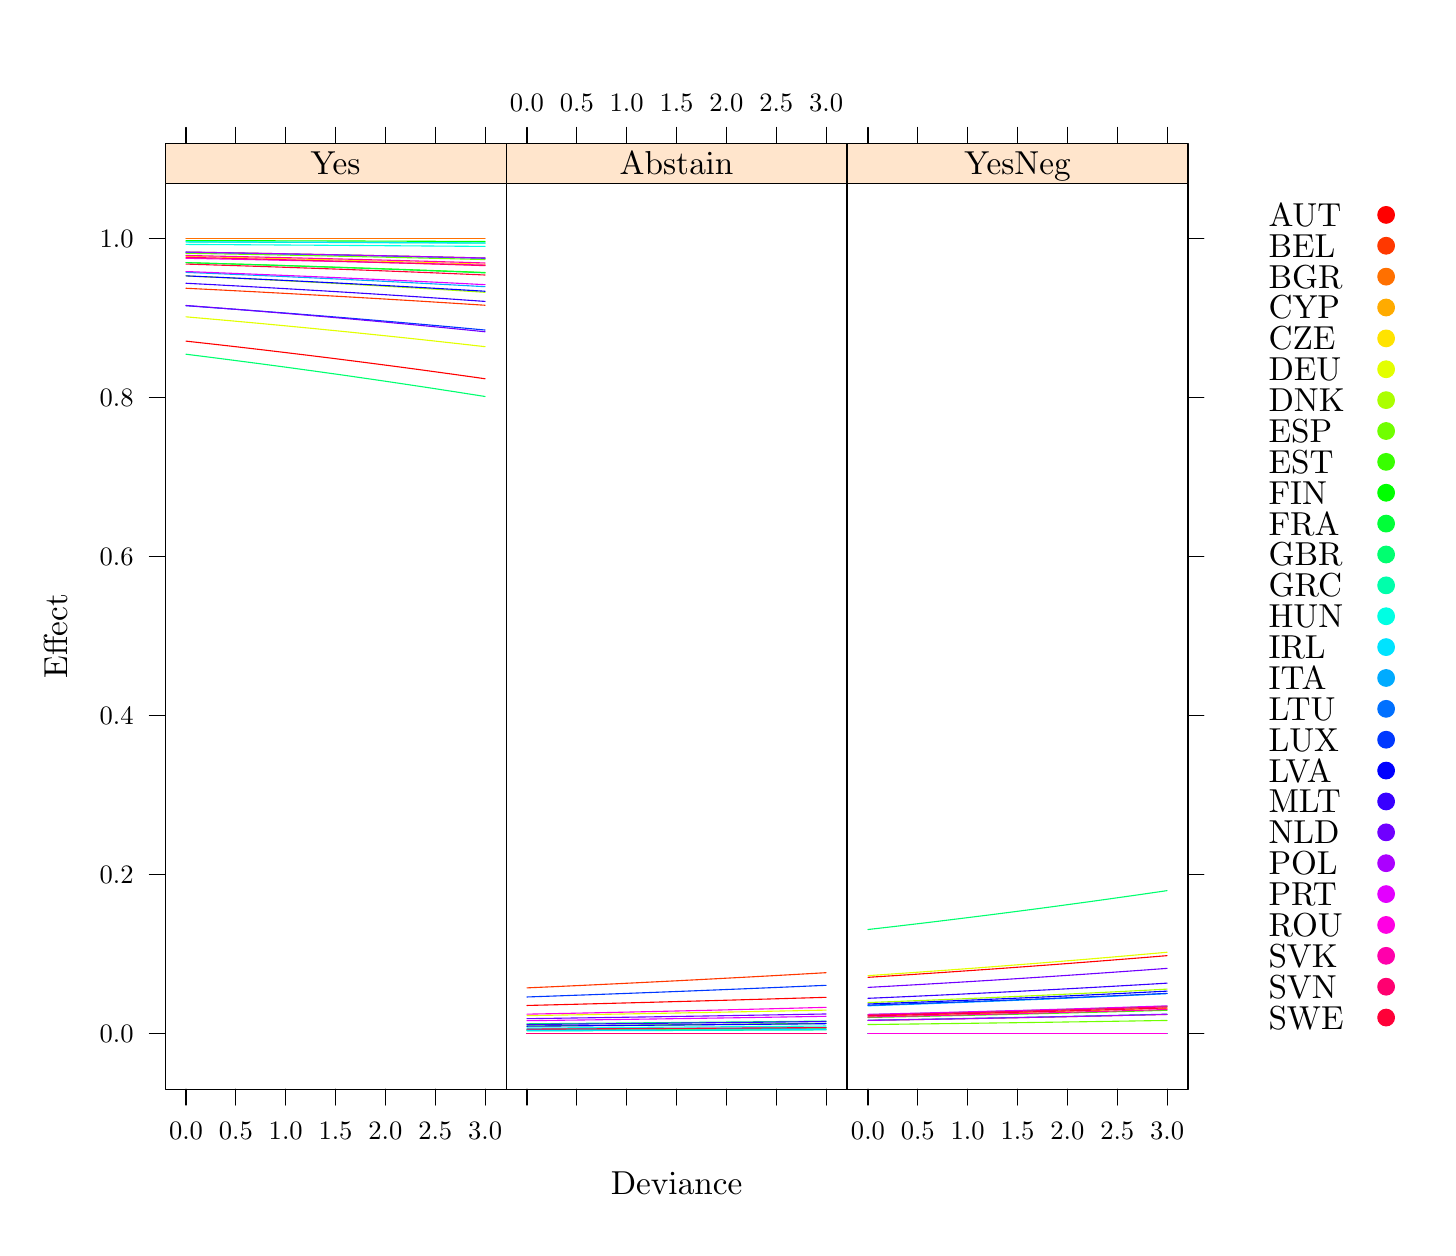
\begin{tikzpicture}[x=1pt,y=1pt]
\definecolor[named]{drawColor}{rgb}{0.00,0.00,0.00}
\definecolor[named]{fillColor}{rgb}{1.00,1.00,1.00}
\fill[color=fillColor,] (0,0) rectangle (505.89,433.62);
\begin{scope}
\path[clip] (  0.00,  0.00) rectangle (505.89,433.62);
\definecolor[named]{fillColor}{rgb}{0.00,0.00,0.00}
\end{scope}
\begin{scope}
\path[clip] (  0.00,  0.00) rectangle (505.89,433.62);
\definecolor[named]{fillColor}{rgb}{0.00,0.00,0.00}

\draw[fill opacity=0.00,draw opacity=0.00,] (  0.00,  0.00) rectangle (505.89,433.62);
\end{scope}
\begin{scope}
\path[clip] (  0.00,  0.00) rectangle (505.89,433.62);
\definecolor[named]{fillColor}{rgb}{0.00,0.00,0.00}
\end{scope}
\begin{scope}
\path[clip] (  0.00,  0.00) rectangle (505.89,433.62);
\definecolor[named]{fillColor}{rgb}{0.00,0.00,0.00}
\definecolor[named]{drawColor}{rgb}{0.00,0.00,0.00}

\node[color=drawColor,anchor=base,inner sep=0pt, outer sep=0pt, scale=  1.20] at (234.47, 12.04) {Deviance%
};
\end{scope}
\begin{scope}
\path[clip] (  0.00,  0.00) rectangle (505.89,433.62);
\definecolor[named]{fillColor}{rgb}{0.00,0.00,0.00}
\definecolor[named]{drawColor}{rgb}{0.00,0.00,0.00}

\node[rotate= 90.00,color=drawColor,anchor=base,inner sep=0pt, outer sep=0pt, scale=  1.20] at ( 14.29,213.72) {Effect%
};
\end{scope}
\begin{scope}
\path[clip] (  0.00,  0.00) rectangle (505.89,433.62);
\definecolor[named]{fillColor}{rgb}{0.00,0.00,0.00}
\end{scope}
\begin{scope}
\path[clip] (  0.00,  0.00) rectangle (505.89,433.62);
\definecolor[named]{fillColor}{rgb}{0.00,0.00,0.00}
\end{scope}
\begin{scope}
\path[clip] (  0.00,  0.00) rectangle (505.89,433.62);
\definecolor[named]{fillColor}{rgb}{0.00,0.00,0.00}
\end{scope}
\begin{scope}
\path[clip] ( 49.65, 50.02) rectangle (172.86,377.42);
\definecolor[named]{fillColor}{rgb}{0.00,0.00,0.00}
\end{scope}
\begin{scope}
\path[clip] (  0.00,  0.00) rectangle (505.89,433.62);
\definecolor[named]{fillColor}{rgb}{0.00,0.00,0.00}
\end{scope}
\begin{scope}
\path[clip] (  0.00,  0.00) rectangle (505.89,433.62);
\definecolor[named]{fillColor}{rgb}{0.00,0.00,0.00}
\definecolor[named]{drawColor}{rgb}{0.00,0.00,0.00}

\draw[color=drawColor,line cap=round,line join=round,fill opacity=0.00,] ( 57.21,391.87) -- ( 57.21,397.56);

\draw[color=drawColor,line cap=round,line join=round,fill opacity=0.00,] ( 75.22,391.87) -- ( 75.22,397.56);

\draw[color=drawColor,line cap=round,line join=round,fill opacity=0.00,] ( 93.24,391.87) -- ( 93.24,397.56);

\draw[color=drawColor,line cap=round,line join=round,fill opacity=0.00,] (111.25,391.87) -- (111.25,397.56);

\draw[color=drawColor,line cap=round,line join=round,fill opacity=0.00,] (129.27,391.87) -- (129.27,397.56);

\draw[color=drawColor,line cap=round,line join=round,fill opacity=0.00,] (147.28,391.87) -- (147.28,397.56);

\draw[color=drawColor,line cap=round,line join=round,fill opacity=0.00,] (165.29,391.87) -- (165.29,397.56);
\end{scope}
\begin{scope}
\path[clip] (  0.00,  0.00) rectangle (505.89,433.62);
\definecolor[named]{fillColor}{rgb}{0.00,0.00,0.00}
\end{scope}
\begin{scope}
\path[clip] (  0.00,  0.00) rectangle (505.89,433.62);
\definecolor[named]{fillColor}{rgb}{0.00,0.00,0.00}
\definecolor[named]{drawColor}{rgb}{0.00,0.00,0.00}

\draw[color=drawColor,line cap=round,line join=round,fill opacity=0.00,] ( 49.65, 70.12) -- ( 43.95, 70.12);

\draw[color=drawColor,line cap=round,line join=round,fill opacity=0.00,] ( 49.65,127.56) -- ( 43.95,127.56);

\draw[color=drawColor,line cap=round,line join=round,fill opacity=0.00,] ( 49.65,185.00) -- ( 43.95,185.00);

\draw[color=drawColor,line cap=round,line join=round,fill opacity=0.00,] ( 49.65,242.43) -- ( 43.95,242.43);

\draw[color=drawColor,line cap=round,line join=round,fill opacity=0.00,] ( 49.65,299.87) -- ( 43.95,299.87);

\draw[color=drawColor,line cap=round,line join=round,fill opacity=0.00,] ( 49.65,357.31) -- ( 43.95,357.31);

\node[color=drawColor,anchor=base east,inner sep=0pt, outer sep=0pt, scale=  0.96] at ( 38.26, 66.81) {0.0%
};

\node[color=drawColor,anchor=base east,inner sep=0pt, outer sep=0pt, scale=  0.96] at ( 38.26,124.25) {0.2%
};

\node[color=drawColor,anchor=base east,inner sep=0pt, outer sep=0pt, scale=  0.96] at ( 38.26,181.69) {0.4%
};

\node[color=drawColor,anchor=base east,inner sep=0pt, outer sep=0pt, scale=  0.96] at ( 38.26,239.13) {0.6%
};

\node[color=drawColor,anchor=base east,inner sep=0pt, outer sep=0pt, scale=  0.96] at ( 38.26,296.57) {0.8%
};

\node[color=drawColor,anchor=base east,inner sep=0pt, outer sep=0pt, scale=  0.96] at ( 38.26,354.01) {1.0%
};
\end{scope}
\begin{scope}
\path[clip] (  0.00,  0.00) rectangle (505.89,433.62);
\definecolor[named]{fillColor}{rgb}{0.00,0.00,0.00}
\end{scope}
\begin{scope}
\path[clip] (  0.00,  0.00) rectangle (505.89,433.62);
\definecolor[named]{fillColor}{rgb}{0.00,0.00,0.00}
\definecolor[named]{drawColor}{rgb}{0.00,0.00,0.00}

\draw[color=drawColor,line cap=round,line join=round,fill opacity=0.00,] ( 57.21, 50.02) -- ( 57.21, 44.32);

\draw[color=drawColor,line cap=round,line join=round,fill opacity=0.00,] ( 75.22, 50.02) -- ( 75.22, 44.32);

\draw[color=drawColor,line cap=round,line join=round,fill opacity=0.00,] ( 93.24, 50.02) -- ( 93.24, 44.32);

\draw[color=drawColor,line cap=round,line join=round,fill opacity=0.00,] (111.25, 50.02) -- (111.25, 44.32);

\draw[color=drawColor,line cap=round,line join=round,fill opacity=0.00,] (129.27, 50.02) -- (129.27, 44.32);

\draw[color=drawColor,line cap=round,line join=round,fill opacity=0.00,] (147.28, 50.02) -- (147.28, 44.32);

\draw[color=drawColor,line cap=round,line join=round,fill opacity=0.00,] (165.29, 50.02) -- (165.29, 44.32);

\node[color=drawColor,anchor=base,inner sep=0pt, outer sep=0pt, scale=  0.96] at ( 57.21, 32.02) {0.0%
};

\node[color=drawColor,anchor=base,inner sep=0pt, outer sep=0pt, scale=  0.96] at ( 75.22, 32.02) {0.5%
};

\node[color=drawColor,anchor=base,inner sep=0pt, outer sep=0pt, scale=  0.96] at ( 93.24, 32.02) {1.0%
};

\node[color=drawColor,anchor=base,inner sep=0pt, outer sep=0pt, scale=  0.96] at (111.25, 32.02) {1.5%
};

\node[color=drawColor,anchor=base,inner sep=0pt, outer sep=0pt, scale=  0.96] at (129.27, 32.02) {2.0%
};

\node[color=drawColor,anchor=base,inner sep=0pt, outer sep=0pt, scale=  0.96] at (147.28, 32.02) {2.5%
};

\node[color=drawColor,anchor=base,inner sep=0pt, outer sep=0pt, scale=  0.96] at (165.29, 32.02) {3.0%
};
\end{scope}
\begin{scope}
\path[clip] (  0.00,  0.00) rectangle (505.89,433.62);
\definecolor[named]{fillColor}{rgb}{0.00,0.00,0.00}
\end{scope}
\begin{scope}
\path[clip] ( 49.65, 50.02) rectangle (172.86,377.42);
\definecolor[named]{fillColor}{rgb}{0.00,0.00,0.00}
\definecolor[named]{drawColor}{rgb}{1.00,0.00,0.00}

\draw[color=drawColor,line cap=round,line join=round,fill opacity=0.00,] ( 57.21,320.35) --
	( 60.81,319.95) --
	( 64.42,319.55) --
	( 68.02,319.15) --
	( 71.62,318.74) --
	( 75.22,318.33) --
	( 78.83,317.91) --
	( 82.43,317.49) --
	( 86.03,317.07) --
	( 89.64,316.64) --
	( 93.24,316.21) --
	( 96.84,315.77) --
	(100.44,315.34) --
	(104.05,314.89) --
	(107.65,314.45) --
	(111.25,314.00) --
	(114.85,313.54) --
	(118.46,313.08) --
	(122.06,312.62) --
	(125.66,312.15) --
	(129.27,311.68) --
	(132.87,311.21) --
	(136.47,310.73) --
	(140.07,310.25) --
	(143.68,309.76) --
	(147.28,309.27) --
	(150.88,308.77) --
	(154.49,308.28) --
	(158.09,307.77) --
	(161.69,307.27) --
	(165.29,306.75);
\definecolor[named]{drawColor}{rgb}{1.00,0.22,0.00}

\draw[color=drawColor,line cap=round,line join=round,fill opacity=0.00,] ( 57.21,339.45) --
	( 60.81,339.27) --
	( 64.42,339.09) --
	( 68.02,338.91) --
	( 71.62,338.73) --
	( 75.22,338.54) --
	( 78.83,338.35) --
	( 82.43,338.17) --
	( 86.03,337.97) --
	( 89.64,337.78) --
	( 93.24,337.59) --
	( 96.84,337.39) --
	(100.44,337.19) --
	(104.05,337.00) --
	(107.65,336.79) --
	(111.25,336.59) --
	(114.85,336.39) --
	(118.46,336.18) --
	(122.06,335.97) --
	(125.66,335.76) --
	(129.27,335.55) --
	(132.87,335.33) --
	(136.47,335.12) --
	(140.07,334.90) --
	(143.68,334.68) --
	(147.28,334.45) --
	(150.88,334.23) --
	(154.49,334.00) --
	(158.09,333.77) --
	(161.69,333.54) --
	(165.29,333.31);
\definecolor[named]{drawColor}{rgb}{1.00,0.44,0.00}

\draw[color=drawColor,line cap=round,line join=round,fill opacity=0.00,] ( 57.21,357.31) --
	( 60.81,357.31) --
	( 64.42,357.31) --
	( 68.02,357.31) --
	( 71.62,357.31) --
	( 75.22,357.31) --
	( 78.83,357.31) --
	( 82.43,357.31) --
	( 86.03,357.31) --
	( 89.64,357.31) --
	( 93.24,357.31) --
	( 96.84,357.31) --
	(100.44,357.31) --
	(104.05,357.31) --
	(107.65,357.31) --
	(111.25,357.31) --
	(114.85,357.31) --
	(118.46,357.31) --
	(122.06,357.31) --
	(125.66,357.31) --
	(129.27,357.31) --
	(132.87,357.31) --
	(136.47,357.31) --
	(140.07,357.31) --
	(143.68,357.31) --
	(147.28,357.31) --
	(150.88,357.31) --
	(154.49,357.31) --
	(158.09,357.31) --
	(161.69,357.31) --
	(165.29,357.31);
\definecolor[named]{drawColor}{rgb}{1.00,0.67,0.00}

\draw[color=drawColor,line cap=round,line join=round,fill opacity=0.00,] ( 57.21,352.53) --
	( 60.81,352.47) --
	( 64.42,352.41) --
	( 68.02,352.35) --
	( 71.62,352.29) --
	( 75.22,352.23) --
	( 78.83,352.16) --
	( 82.43,352.10) --
	( 86.03,352.03) --
	( 89.64,351.97) --
	( 93.24,351.90) --
	( 96.84,351.83) --
	(100.44,351.76) --
	(104.05,351.69) --
	(107.65,351.62) --
	(111.25,351.55) --
	(114.85,351.48) --
	(118.46,351.40) --
	(122.06,351.33) --
	(125.66,351.26) --
	(129.27,351.18) --
	(132.87,351.10) --
	(136.47,351.03) --
	(140.07,350.95) --
	(143.68,350.87) --
	(147.28,350.79) --
	(150.88,350.71) --
	(154.49,350.62) --
	(158.09,350.54) --
	(161.69,350.45) --
	(165.29,350.37);
\definecolor[named]{drawColor}{rgb}{1.00,0.89,0.00}

\draw[color=drawColor,line cap=round,line join=round,fill opacity=0.00,] ( 57.21,350.98) --
	( 60.81,350.90) --
	( 64.42,350.82) --
	( 68.02,350.74) --
	( 71.62,350.65) --
	( 75.22,350.57) --
	( 78.83,350.49) --
	( 82.43,350.40) --
	( 86.03,350.32) --
	( 89.64,350.23) --
	( 93.24,350.14) --
	( 96.84,350.05) --
	(100.44,349.96) --
	(104.05,349.87) --
	(107.65,349.78) --
	(111.25,349.68) --
	(114.85,349.59) --
	(118.46,349.49) --
	(122.06,349.39) --
	(125.66,349.29) --
	(129.27,349.19) --
	(132.87,349.09) --
	(136.47,348.99) --
	(140.07,348.89) --
	(143.68,348.78) --
	(147.28,348.68) --
	(150.88,348.57) --
	(154.49,348.46) --
	(158.09,348.35) --
	(161.69,348.24) --
	(165.29,348.13);
\definecolor[named]{drawColor}{rgb}{0.89,1.00,0.00}

\draw[color=drawColor,line cap=round,line join=round,fill opacity=0.00,] ( 57.21,329.13) --
	( 60.81,328.81) --
	( 64.42,328.50) --
	( 68.02,328.18) --
	( 71.62,327.86) --
	( 75.22,327.54) --
	( 78.83,327.21) --
	( 82.43,326.88) --
	( 86.03,326.55) --
	( 89.64,326.21) --
	( 93.24,325.87) --
	( 96.84,325.52) --
	(100.44,325.18) --
	(104.05,324.83) --
	(107.65,324.47) --
	(111.25,324.12) --
	(114.85,323.76) --
	(118.46,323.39) --
	(122.06,323.02) --
	(125.66,322.65) --
	(129.27,322.28) --
	(132.87,321.90) --
	(136.47,321.52) --
	(140.07,321.14) --
	(143.68,320.75) --
	(147.28,320.36) --
	(150.88,319.96) --
	(154.49,319.56) --
	(158.09,319.16) --
	(161.69,318.75) --
	(165.29,318.34);
\definecolor[named]{drawColor}{rgb}{0.67,1.00,0.00}

\draw[color=drawColor,line cap=round,line join=round,fill opacity=0.00,] ( 57.21,343.91) --
	( 60.81,343.74) --
	( 64.42,343.58) --
	( 68.02,343.41) --
	( 71.62,343.23) --
	( 75.22,343.06) --
	( 78.83,342.88) --
	( 82.43,342.71) --
	( 86.03,342.53) --
	( 89.64,342.34) --
	( 93.24,342.16) --
	( 96.84,341.97) --
	(100.44,341.78) --
	(104.05,341.59) --
	(107.65,341.40) --
	(111.25,341.20) --
	(114.85,341.01) --
	(118.46,340.81) --
	(122.06,340.60) --
	(125.66,340.40) --
	(129.27,340.19) --
	(132.87,339.98) --
	(136.47,339.77) --
	(140.07,339.56) --
	(143.68,339.34) --
	(147.28,339.12) --
	(150.88,338.90) --
	(154.49,338.68) --
	(158.09,338.45) --
	(161.69,338.22) --
	(165.29,337.99);
\definecolor[named]{drawColor}{rgb}{0.44,1.00,0.00}

\draw[color=drawColor,line cap=round,line join=round,fill opacity=0.00,] ( 57.21,352.10) --
	( 60.81,352.04) --
	( 64.42,351.97) --
	( 68.02,351.91) --
	( 71.62,351.84) --
	( 75.22,351.78) --
	( 78.83,351.71) --
	( 82.43,351.64) --
	( 86.03,351.57) --
	( 89.64,351.50) --
	( 93.24,351.43) --
	( 96.84,351.36) --
	(100.44,351.29) --
	(104.05,351.21) --
	(107.65,351.14) --
	(111.25,351.06) --
	(114.85,350.99) --
	(118.46,350.91) --
	(122.06,350.83) --
	(125.66,350.75) --
	(129.27,350.68) --
	(132.87,350.59) --
	(136.47,350.51) --
	(140.07,350.43) --
	(143.68,350.35) --
	(147.28,350.26) --
	(150.88,350.18) --
	(154.49,350.09) --
	(158.09,350.00) --
	(161.69,349.91) --
	(165.29,349.82);
\definecolor[named]{drawColor}{rgb}{0.22,1.00,0.00}

\draw[color=drawColor,line cap=round,line join=round,fill opacity=0.00,] ( 57.21,348.71) --
	( 60.81,348.61) --
	( 64.42,348.51) --
	( 68.02,348.41) --
	( 71.62,348.30) --
	( 75.22,348.20) --
	( 78.83,348.09) --
	( 82.43,347.98) --
	( 86.03,347.88) --
	( 89.64,347.77) --
	( 93.24,347.65) --
	( 96.84,347.54) --
	(100.44,347.43) --
	(104.05,347.31) --
	(107.65,347.20) --
	(111.25,347.08) --
	(114.85,346.96) --
	(118.46,346.84) --
	(122.06,346.72) --
	(125.66,346.60) --
	(129.27,346.47) --
	(132.87,346.35) --
	(136.47,346.22) --
	(140.07,346.09) --
	(143.68,345.96) --
	(147.28,345.83) --
	(150.88,345.70) --
	(154.49,345.56) --
	(158.09,345.43) --
	(161.69,345.29) --
	(165.29,345.15);
\definecolor[named]{drawColor}{rgb}{0.00,1.00,0.00}

\draw[color=drawColor,line cap=round,line join=round,fill opacity=0.00,] ( 57.21,356.68) --
	( 60.81,356.68) --
	( 64.42,356.67) --
	( 68.02,356.66) --
	( 71.62,356.65) --
	( 75.22,356.64) --
	( 78.83,356.63) --
	( 82.43,356.62) --
	( 86.03,356.61) --
	( 89.64,356.60) --
	( 93.24,356.59) --
	( 96.84,356.58) --
	(100.44,356.57) --
	(104.05,356.56) --
	(107.65,356.55) --
	(111.25,356.54) --
	(114.85,356.53) --
	(118.46,356.52) --
	(122.06,356.51) --
	(125.66,356.49) --
	(129.27,356.48) --
	(132.87,356.47) --
	(136.47,356.46) --
	(140.07,356.45) --
	(143.68,356.44) --
	(147.28,356.42) --
	(150.88,356.41) --
	(154.49,356.40) --
	(158.09,356.39) --
	(161.69,356.37) --
	(165.29,356.36);
\definecolor[named]{drawColor}{rgb}{0.00,1.00,0.22}

\draw[color=drawColor,line cap=round,line join=round,fill opacity=0.00,] ( 57.21,348.71) --
	( 60.81,348.61) --
	( 64.42,348.50) --
	( 68.02,348.39) --
	( 71.62,348.29) --
	( 75.22,348.18) --
	( 78.83,348.07) --
	( 82.43,347.96) --
	( 86.03,347.85) --
	( 89.64,347.73) --
	( 93.24,347.62) --
	( 96.84,347.50) --
	(100.44,347.38) --
	(104.05,347.26) --
	(107.65,347.14) --
	(111.25,347.02) --
	(114.85,346.90) --
	(118.46,346.77) --
	(122.06,346.65) --
	(125.66,346.52) --
	(129.27,346.39) --
	(132.87,346.26) --
	(136.47,346.13) --
	(140.07,346.00) --
	(143.68,345.86) --
	(147.28,345.72) --
	(150.88,345.59) --
	(154.49,345.45) --
	(158.09,345.31) --
	(161.69,345.16) --
	(165.29,345.02);
\definecolor[named]{drawColor}{rgb}{0.00,1.00,0.44}

\draw[color=drawColor,line cap=round,line join=round,fill opacity=0.00,] ( 57.21,315.61) --
	( 60.81,315.16) --
	( 64.42,314.71) --
	( 68.02,314.25) --
	( 71.62,313.79) --
	( 75.22,313.32) --
	( 78.83,312.85) --
	( 82.43,312.38) --
	( 86.03,311.90) --
	( 89.64,311.42) --
	( 93.24,310.94) --
	( 96.84,310.45) --
	(100.44,309.95) --
	(104.05,309.46) --
	(107.65,308.95) --
	(111.25,308.45) --
	(114.85,307.94) --
	(118.46,307.42) --
	(122.06,306.90) --
	(125.66,306.38) --
	(129.27,305.85) --
	(132.87,305.32) --
	(136.47,304.78) --
	(140.07,304.24) --
	(143.68,303.70) --
	(147.28,303.15) --
	(150.88,302.59) --
	(154.49,302.04) --
	(158.09,301.47) --
	(161.69,300.91) --
	(165.29,300.34);
\definecolor[named]{drawColor}{rgb}{0.00,1.00,0.67}

\draw[color=drawColor,line cap=round,line join=round,fill opacity=0.00,] ( 57.21,356.19) --
	( 60.81,356.18) --
	( 64.42,356.17) --
	( 68.02,356.15) --
	( 71.62,356.14) --
	( 75.22,356.13) --
	( 78.83,356.12) --
	( 82.43,356.10) --
	( 86.03,356.09) --
	( 89.64,356.08) --
	( 93.24,356.06) --
	( 96.84,356.05) --
	(100.44,356.04) --
	(104.05,356.02) --
	(107.65,356.01) --
	(111.25,356.00) --
	(114.85,355.98) --
	(118.46,355.97) --
	(122.06,355.95) --
	(125.66,355.94) --
	(129.27,355.92) --
	(132.87,355.91) --
	(136.47,355.89) --
	(140.07,355.88) --
	(143.68,355.86) --
	(147.28,355.85) --
	(150.88,355.83) --
	(154.49,355.81) --
	(158.09,355.80) --
	(161.69,355.78) --
	(165.29,355.77);
\definecolor[named]{drawColor}{rgb}{0.00,1.00,0.89}

\draw[color=drawColor,line cap=round,line join=round,fill opacity=0.00,] ( 57.21,355.29) --
	( 60.81,355.27) --
	( 64.42,355.25) --
	( 68.02,355.23) --
	( 71.62,355.21) --
	( 75.22,355.19) --
	( 78.83,355.17) --
	( 82.43,355.14) --
	( 86.03,355.12) --
	( 89.64,355.10) --
	( 93.24,355.08) --
	( 96.84,355.05) --
	(100.44,355.03) --
	(104.05,355.01) --
	(107.65,354.98) --
	(111.25,354.96) --
	(114.85,354.93) --
	(118.46,354.91) --
	(122.06,354.88) --
	(125.66,354.86) --
	(129.27,354.83) --
	(132.87,354.81) --
	(136.47,354.78) --
	(140.07,354.76) --
	(143.68,354.73) --
	(147.28,354.70) --
	(150.88,354.68) --
	(154.49,354.65) --
	(158.09,354.62) --
	(161.69,354.60) --
	(165.29,354.57);
\definecolor[named]{drawColor}{rgb}{0.00,0.89,1.00}

\draw[color=drawColor,line cap=round,line join=round,fill opacity=0.00,] ( 57.21,356.23) --
	( 60.81,356.22) --
	( 64.42,356.21) --
	( 68.02,356.19) --
	( 71.62,356.18) --
	( 75.22,356.17) --
	( 78.83,356.16) --
	( 82.43,356.15) --
	( 86.03,356.14) --
	( 89.64,356.12) --
	( 93.24,356.11) --
	( 96.84,356.10) --
	(100.44,356.09) --
	(104.05,356.07) --
	(107.65,356.06) --
	(111.25,356.05) --
	(114.85,356.03) --
	(118.46,356.02) --
	(122.06,356.01) --
	(125.66,355.99) --
	(129.27,355.98) --
	(132.87,355.97) --
	(136.47,355.95) --
	(140.07,355.94) --
	(143.68,355.92) --
	(147.28,355.91) --
	(150.88,355.90) --
	(154.49,355.88) --
	(158.09,355.87) --
	(161.69,355.85) --
	(165.29,355.84);
\definecolor[named]{drawColor}{rgb}{0.00,0.67,1.00}

\draw[color=drawColor,line cap=round,line join=round,fill opacity=0.00,] ( 57.21,345.19) --
	( 60.81,345.04) --
	( 64.42,344.90) --
	( 68.02,344.75) --
	( 71.62,344.60) --
	( 75.22,344.44) --
	( 78.83,344.29) --
	( 82.43,344.13) --
	( 86.03,343.98) --
	( 89.64,343.82) --
	( 93.24,343.66) --
	( 96.84,343.49) --
	(100.44,343.33) --
	(104.05,343.16) --
	(107.65,342.99) --
	(111.25,342.82) --
	(114.85,342.65) --
	(118.46,342.47) --
	(122.06,342.30) --
	(125.66,342.12) --
	(129.27,341.94) --
	(132.87,341.76) --
	(136.47,341.57) --
	(140.07,341.38) --
	(143.68,341.20) --
	(147.28,341.00) --
	(150.88,340.81) --
	(154.49,340.62) --
	(158.09,340.42) --
	(161.69,340.22) --
	(165.29,340.02);
\definecolor[named]{drawColor}{rgb}{0.00,0.44,1.00}

\draw[color=drawColor,line cap=round,line join=round,fill opacity=0.00,] ( 57.21,352.47) --
	( 60.81,352.41) --
	( 64.42,352.35) --
	( 68.02,352.29) --
	( 71.62,352.23) --
	( 75.22,352.16) --
	( 78.83,352.10) --
	( 82.43,352.03) --
	( 86.03,351.97) --
	( 89.64,351.90) --
	( 93.24,351.83) --
	( 96.84,351.76) --
	(100.44,351.69) --
	(104.05,351.62) --
	(107.65,351.55) --
	(111.25,351.48) --
	(114.85,351.41) --
	(118.46,351.33) --
	(122.06,351.26) --
	(125.66,351.18) --
	(129.27,351.10) --
	(132.87,351.03) --
	(136.47,350.95) --
	(140.07,350.87) --
	(143.68,350.79) --
	(147.28,350.71) --
	(150.88,350.62) --
	(154.49,350.54) --
	(158.09,350.45) --
	(161.69,350.37) --
	(165.29,350.28);
\definecolor[named]{drawColor}{rgb}{0.00,0.22,1.00}

\draw[color=drawColor,line cap=round,line join=round,fill opacity=0.00,] ( 57.21,333.15) --
	( 60.81,332.89) --
	( 64.42,332.63) --
	( 68.02,332.37) --
	( 71.62,332.11) --
	( 75.22,331.85) --
	( 78.83,331.58) --
	( 82.43,331.31) --
	( 86.03,331.04) --
	( 89.64,330.76) --
	( 93.24,330.49) --
	( 96.84,330.21) --
	(100.44,329.92) --
	(104.05,329.64) --
	(107.65,329.35) --
	(111.25,329.06) --
	(114.85,328.77) --
	(118.46,328.47) --
	(122.06,328.17) --
	(125.66,327.87) --
	(129.27,327.56) --
	(132.87,327.26) --
	(136.47,326.95) --
	(140.07,326.63) --
	(143.68,326.32) --
	(147.28,326.00) --
	(150.88,325.68) --
	(154.49,325.35) --
	(158.09,325.02) --
	(161.69,324.69) --
	(165.29,324.36);
\definecolor[named]{drawColor}{rgb}{0.00,0.00,1.00}

\draw[color=drawColor,line cap=round,line join=round,fill opacity=0.00,] ( 57.21,343.93) --
	( 60.81,343.77) --
	( 64.42,343.61) --
	( 68.02,343.45) --
	( 71.62,343.29) --
	( 75.22,343.13) --
	( 78.83,342.96) --
	( 82.43,342.79) --
	( 86.03,342.62) --
	( 89.64,342.45) --
	( 93.24,342.28) --
	( 96.84,342.10) --
	(100.44,341.92) --
	(104.05,341.74) --
	(107.65,341.56) --
	(111.25,341.38) --
	(114.85,341.19) --
	(118.46,341.01) --
	(122.06,340.82) --
	(125.66,340.63) --
	(129.27,340.43) --
	(132.87,340.24) --
	(136.47,340.04) --
	(140.07,339.84) --
	(143.68,339.64) --
	(147.28,339.43) --
	(150.88,339.22) --
	(154.49,339.02) --
	(158.09,338.80) --
	(161.69,338.59) --
	(165.29,338.37);
\definecolor[named]{drawColor}{rgb}{0.22,0.00,1.00}

\draw[color=drawColor,line cap=round,line join=round,fill opacity=0.00,] ( 57.21,341.26) --
	( 60.81,341.07) --
	( 64.42,340.89) --
	( 68.02,340.70) --
	( 71.62,340.50) --
	( 75.22,340.31) --
	( 78.83,340.11) --
	( 82.43,339.91) --
	( 86.03,339.71) --
	( 89.64,339.51) --
	( 93.24,339.30) --
	( 96.84,339.09) --
	(100.44,338.88) --
	(104.05,338.67) --
	(107.65,338.46) --
	(111.25,338.24) --
	(114.85,338.02) --
	(118.46,337.80) --
	(122.06,337.58) --
	(125.66,337.35) --
	(129.27,337.12) --
	(132.87,336.89) --
	(136.47,336.66) --
	(140.07,336.42) --
	(143.68,336.18) --
	(147.28,335.94) --
	(150.88,335.70) --
	(154.49,335.45) --
	(158.09,335.20) --
	(161.69,334.95) --
	(165.29,334.70);
\definecolor[named]{drawColor}{rgb}{0.44,0.00,1.00}

\draw[color=drawColor,line cap=round,line join=round,fill opacity=0.00,] ( 57.21,333.23) --
	( 60.81,332.96) --
	( 64.42,332.68) --
	( 68.02,332.40) --
	( 71.62,332.12) --
	( 75.22,331.84) --
	( 78.83,331.55) --
	( 82.43,331.26) --
	( 86.03,330.97) --
	( 89.64,330.67) --
	( 93.24,330.37) --
	( 96.84,330.07) --
	(100.44,329.77) --
	(104.05,329.46) --
	(107.65,329.15) --
	(111.25,328.83) --
	(114.85,328.52) --
	(118.46,328.20) --
	(122.06,327.87) --
	(125.66,327.55) --
	(129.27,327.22) --
	(132.87,326.88) --
	(136.47,326.55) --
	(140.07,326.21) --
	(143.68,325.86) --
	(147.28,325.52) --
	(150.88,325.17) --
	(154.49,324.81) --
	(158.09,324.46) --
	(161.69,324.10) --
	(165.29,323.73);
\definecolor[named]{drawColor}{rgb}{0.67,0.00,1.00}

\draw[color=drawColor,line cap=round,line join=round,fill opacity=0.00,] ( 57.21,352.54) --
	( 60.81,352.48) --
	( 64.42,352.42) --
	( 68.02,352.36) --
	( 71.62,352.30) --
	( 75.22,352.23) --
	( 78.83,352.17) --
	( 82.43,352.10) --
	( 86.03,352.04) --
	( 89.64,351.97) --
	( 93.24,351.90) --
	( 96.84,351.84) --
	(100.44,351.77) --
	(104.05,351.70) --
	(107.65,351.63) --
	(111.25,351.56) --
	(114.85,351.48) --
	(118.46,351.41) --
	(122.06,351.34) --
	(125.66,351.26) --
	(129.27,351.19) --
	(132.87,351.11) --
	(136.47,351.03) --
	(140.07,350.95) --
	(143.68,350.87) --
	(147.28,350.79) --
	(150.88,350.71) --
	(154.49,350.63) --
	(158.09,350.55) --
	(161.69,350.46) --
	(165.29,350.38);
\definecolor[named]{drawColor}{rgb}{0.89,0.00,1.00}

\draw[color=drawColor,line cap=round,line join=round,fill opacity=0.00,] ( 57.21,345.49) --
	( 60.81,345.36) --
	( 64.42,345.22) --
	( 68.02,345.08) --
	( 71.62,344.94) --
	( 75.22,344.80) --
	( 78.83,344.66) --
	( 82.43,344.52) --
	( 86.03,344.37) --
	( 89.64,344.23) --
	( 93.24,344.08) --
	( 96.84,343.93) --
	(100.44,343.78) --
	(104.05,343.62) --
	(107.65,343.47) --
	(111.25,343.31) --
	(114.85,343.15) --
	(118.46,342.99) --
	(122.06,342.83) --
	(125.66,342.67) --
	(129.27,342.50) --
	(132.87,342.34) --
	(136.47,342.17) --
	(140.07,342.00) --
	(143.68,341.82) --
	(147.28,341.65) --
	(150.88,341.47) --
	(154.49,341.30) --
	(158.09,341.12) --
	(161.69,340.93) --
	(165.29,340.75);
\definecolor[named]{drawColor}{rgb}{1.00,0.00,0.89}

\draw[color=drawColor,line cap=round,line join=round,fill opacity=0.00,] ( 57.21,350.29) --
	( 60.81,350.21) --
	( 64.42,350.14) --
	( 68.02,350.07) --
	( 71.62,350.00) --
	( 75.22,349.92) --
	( 78.83,349.85) --
	( 82.43,349.77) --
	( 86.03,349.70) --
	( 89.64,349.62) --
	( 93.24,349.54) --
	( 96.84,349.46) --
	(100.44,349.38) --
	(104.05,349.30) --
	(107.65,349.22) --
	(111.25,349.14) --
	(114.85,349.06) --
	(118.46,348.98) --
	(122.06,348.89) --
	(125.66,348.81) --
	(129.27,348.72) --
	(132.87,348.63) --
	(136.47,348.55) --
	(140.07,348.46) --
	(143.68,348.37) --
	(147.28,348.28) --
	(150.88,348.19) --
	(154.49,348.10) --
	(158.09,348.00) --
	(161.69,347.91) --
	(165.29,347.82);
\definecolor[named]{drawColor}{rgb}{1.00,0.00,0.67}

\draw[color=drawColor,line cap=round,line join=round,fill opacity=0.00,] ( 57.21,351.30) --
	( 60.81,351.23) --
	( 64.42,351.15) --
	( 68.02,351.07) --
	( 71.62,351.00) --
	( 75.22,350.92) --
	( 78.83,350.84) --
	( 82.43,350.76) --
	( 86.03,350.67) --
	( 89.64,350.59) --
	( 93.24,350.51) --
	( 96.84,350.42) --
	(100.44,350.34) --
	(104.05,350.25) --
	(107.65,350.16) --
	(111.25,350.07) --
	(114.85,349.98) --
	(118.46,349.89) --
	(122.06,349.80) --
	(125.66,349.70) --
	(129.27,349.61) --
	(132.87,349.51) --
	(136.47,349.42) --
	(140.07,349.32) --
	(143.68,349.22) --
	(147.28,349.12) --
	(150.88,349.01) --
	(154.49,348.91) --
	(158.09,348.81) --
	(161.69,348.70) --
	(165.29,348.59);
\definecolor[named]{drawColor}{rgb}{1.00,0.00,0.44}

\draw[color=drawColor,line cap=round,line join=round,fill opacity=0.00,] ( 57.21,350.62) --
	( 60.81,350.54) --
	( 64.42,350.46) --
	( 68.02,350.37) --
	( 71.62,350.28) --
	( 75.22,350.20) --
	( 78.83,350.11) --
	( 82.43,350.02) --
	( 86.03,349.93) --
	( 89.64,349.83) --
	( 93.24,349.74) --
	( 96.84,349.65) --
	(100.44,349.55) --
	(104.05,349.45) --
	(107.65,349.36) --
	(111.25,349.26) --
	(114.85,349.16) --
	(118.46,349.06) --
	(122.06,348.95) --
	(125.66,348.85) --
	(129.27,348.74) --
	(132.87,348.64) --
	(136.47,348.53) --
	(140.07,348.42) --
	(143.68,348.31) --
	(147.28,348.20) --
	(150.88,348.09) --
	(154.49,347.97) --
	(158.09,347.86) --
	(161.69,347.74) --
	(165.29,347.62);
\definecolor[named]{drawColor}{rgb}{1.00,0.00,0.22}

\draw[color=drawColor,line cap=round,line join=round,fill opacity=0.00,] ( 57.21,348.19) --
	( 60.81,348.08) --
	( 64.42,347.97) --
	( 68.02,347.85) --
	( 71.62,347.74) --
	( 75.22,347.62) --
	( 78.83,347.51) --
	( 82.43,347.39) --
	( 86.03,347.27) --
	( 89.64,347.15) --
	( 93.24,347.02) --
	( 96.84,346.90) --
	(100.44,346.77) --
	(104.05,346.65) --
	(107.65,346.52) --
	(111.25,346.39) --
	(114.85,346.26) --
	(118.46,346.12) --
	(122.06,345.99) --
	(125.66,345.85) --
	(129.27,345.71) --
	(132.87,345.57) --
	(136.47,345.43) --
	(140.07,345.29) --
	(143.68,345.15) --
	(147.28,345.00) --
	(150.88,344.85) --
	(154.49,344.70) --
	(158.09,344.55) --
	(161.69,344.40) --
	(165.29,344.24);
\end{scope}
\begin{scope}
\path[clip] (  0.00,  0.00) rectangle (505.89,433.62);
\definecolor[named]{fillColor}{rgb}{0.00,0.00,0.00}
\end{scope}
\begin{scope}
\path[clip] (  0.00,  0.00) rectangle (505.89,433.62);
\definecolor[named]{fillColor}{rgb}{0.00,0.00,0.00}
\definecolor[named]{drawColor}{rgb}{0.00,0.00,0.00}

\draw[color=drawColor,line cap=round,line join=round,fill opacity=0.00,] ( 49.65, 50.02) rectangle (172.86,377.42);
\end{scope}
\begin{scope}
\path[clip] (  0.00,  0.00) rectangle (505.89,433.62);
\definecolor[named]{fillColor}{rgb}{0.00,0.00,0.00}
\end{scope}
\begin{scope}
\path[clip] (  0.00,  0.00) rectangle (505.89,433.62);
\definecolor[named]{fillColor}{rgb}{0.00,0.00,0.00}
\end{scope}
\begin{scope}
\path[clip] ( 49.65,377.42) rectangle (172.86,391.87);
\definecolor[named]{fillColor}{rgb}{0.00,0.00,0.00}
\definecolor[named]{drawColor}{rgb}{1.00,0.90,0.80}
\definecolor[named]{fillColor}{rgb}{1.00,0.90,0.80}

\draw[color=drawColor,line cap=round,line join=round,fill=fillColor,] ( 49.65,377.42) rectangle (172.86,391.87);
\definecolor[named]{drawColor}{rgb}{0.00,0.00,0.00}

\node[color=drawColor,anchor=base west,inner sep=0pt, outer sep=0pt, scale=  1.20] at (102.22,380.51) {Yes%
};
\end{scope}
\begin{scope}
\path[clip] (  0.00,  0.00) rectangle (505.89,433.62);
\definecolor[named]{fillColor}{rgb}{0.00,0.00,0.00}
\end{scope}
\begin{scope}
\path[clip] (  0.00,  0.00) rectangle (505.89,433.62);
\definecolor[named]{fillColor}{rgb}{0.00,0.00,0.00}
\definecolor[named]{drawColor}{rgb}{0.00,0.00,0.00}

\draw[color=drawColor,line cap=round,line join=round,fill opacity=0.00,] ( 49.65,377.42) rectangle (172.86,391.87);
\end{scope}
\begin{scope}
\path[clip] (  0.00,  0.00) rectangle (505.89,433.62);
\definecolor[named]{fillColor}{rgb}{0.00,0.00,0.00}
\end{scope}
\begin{scope}
\path[clip] (  0.00,  0.00) rectangle (505.89,433.62);
\definecolor[named]{fillColor}{rgb}{0.00,0.00,0.00}
\end{scope}
\begin{scope}
\path[clip] (172.86, 50.02) rectangle (296.07,377.42);
\definecolor[named]{fillColor}{rgb}{0.00,0.00,0.00}
\end{scope}
\begin{scope}
\path[clip] (  0.00,  0.00) rectangle (505.89,433.62);
\definecolor[named]{fillColor}{rgb}{0.00,0.00,0.00}
\end{scope}
\begin{scope}
\path[clip] (  0.00,  0.00) rectangle (505.89,433.62);
\definecolor[named]{fillColor}{rgb}{0.00,0.00,0.00}
\definecolor[named]{drawColor}{rgb}{0.00,0.00,0.00}

\draw[color=drawColor,line cap=round,line join=round,fill opacity=0.00,] (180.42,391.87) -- (180.42,397.56);

\draw[color=drawColor,line cap=round,line join=round,fill opacity=0.00,] (198.44,391.87) -- (198.44,397.56);

\draw[color=drawColor,line cap=round,line join=round,fill opacity=0.00,] (216.45,391.87) -- (216.45,397.56);

\draw[color=drawColor,line cap=round,line join=round,fill opacity=0.00,] (234.47,391.87) -- (234.47,397.56);

\draw[color=drawColor,line cap=round,line join=round,fill opacity=0.00,] (252.48,391.87) -- (252.48,397.56);

\draw[color=drawColor,line cap=round,line join=round,fill opacity=0.00,] (270.49,391.87) -- (270.49,397.56);

\draw[color=drawColor,line cap=round,line join=round,fill opacity=0.00,] (288.51,391.87) -- (288.51,397.56);

\node[color=drawColor,anchor=base,inner sep=0pt, outer sep=0pt, scale=  0.96] at (180.42,403.25) {0.0%
};

\node[color=drawColor,anchor=base,inner sep=0pt, outer sep=0pt, scale=  0.96] at (198.44,403.25) {0.5%
};

\node[color=drawColor,anchor=base,inner sep=0pt, outer sep=0pt, scale=  0.96] at (216.45,403.25) {1.0%
};

\node[color=drawColor,anchor=base,inner sep=0pt, outer sep=0pt, scale=  0.96] at (234.47,403.25) {1.5%
};

\node[color=drawColor,anchor=base,inner sep=0pt, outer sep=0pt, scale=  0.96] at (252.48,403.25) {2.0%
};

\node[color=drawColor,anchor=base,inner sep=0pt, outer sep=0pt, scale=  0.96] at (270.49,403.25) {2.5%
};

\node[color=drawColor,anchor=base,inner sep=0pt, outer sep=0pt, scale=  0.96] at (288.51,403.25) {3.0%
};
\end{scope}
\begin{scope}
\path[clip] (  0.00,  0.00) rectangle (505.89,433.62);
\definecolor[named]{fillColor}{rgb}{0.00,0.00,0.00}
\end{scope}
\begin{scope}
\path[clip] (  0.00,  0.00) rectangle (505.89,433.62);
\definecolor[named]{fillColor}{rgb}{0.00,0.00,0.00}
\end{scope}
\begin{scope}
\path[clip] (  0.00,  0.00) rectangle (505.89,433.62);
\definecolor[named]{fillColor}{rgb}{0.00,0.00,0.00}
\end{scope}
\begin{scope}
\path[clip] (  0.00,  0.00) rectangle (505.89,433.62);
\definecolor[named]{fillColor}{rgb}{0.00,0.00,0.00}
\definecolor[named]{drawColor}{rgb}{0.00,0.00,0.00}

\draw[color=drawColor,line cap=round,line join=round,fill opacity=0.00,] (180.42, 50.02) -- (180.42, 44.32);

\draw[color=drawColor,line cap=round,line join=round,fill opacity=0.00,] (198.44, 50.02) -- (198.44, 44.32);

\draw[color=drawColor,line cap=round,line join=round,fill opacity=0.00,] (216.45, 50.02) -- (216.45, 44.32);

\draw[color=drawColor,line cap=round,line join=round,fill opacity=0.00,] (234.47, 50.02) -- (234.47, 44.32);

\draw[color=drawColor,line cap=round,line join=round,fill opacity=0.00,] (252.48, 50.02) -- (252.48, 44.32);

\draw[color=drawColor,line cap=round,line join=round,fill opacity=0.00,] (270.49, 50.02) -- (270.49, 44.32);

\draw[color=drawColor,line cap=round,line join=round,fill opacity=0.00,] (288.51, 50.02) -- (288.51, 44.32);
\end{scope}
\begin{scope}
\path[clip] (  0.00,  0.00) rectangle (505.89,433.62);
\definecolor[named]{fillColor}{rgb}{0.00,0.00,0.00}
\end{scope}
\begin{scope}
\path[clip] (172.86, 50.02) rectangle (296.07,377.42);
\definecolor[named]{fillColor}{rgb}{0.00,0.00,0.00}
\definecolor[named]{drawColor}{rgb}{1.00,0.00,0.00}

\draw[color=drawColor,line cap=round,line join=round,fill opacity=0.00,] (180.42, 80.29) --
	(184.03, 80.38) --
	(187.63, 80.47) --
	(191.23, 80.56) --
	(194.84, 80.65) --
	(198.44, 80.74) --
	(202.04, 80.84) --
	(205.64, 80.93) --
	(209.25, 81.02) --
	(212.85, 81.12) --
	(216.45, 81.21) --
	(220.06, 81.31) --
	(223.66, 81.40) --
	(227.26, 81.50) --
	(230.86, 81.60) --
	(234.47, 81.70) --
	(238.07, 81.79) --
	(241.67, 81.89) --
	(245.27, 81.99) --
	(248.88, 82.09) --
	(252.48, 82.19) --
	(256.08, 82.29) --
	(259.69, 82.40) --
	(263.29, 82.50) --
	(266.89, 82.60) --
	(270.49, 82.71) --
	(274.10, 82.81) --
	(277.70, 82.92) --
	(281.30, 83.02) --
	(284.90, 83.13) --
	(288.51, 83.23);
\definecolor[named]{drawColor}{rgb}{1.00,0.22,0.00}

\draw[color=drawColor,line cap=round,line join=round,fill opacity=0.00,] (180.42, 86.65) --
	(184.03, 86.81) --
	(187.63, 86.97) --
	(191.23, 87.13) --
	(194.84, 87.30) --
	(198.44, 87.46) --
	(202.04, 87.63) --
	(205.64, 87.80) --
	(209.25, 87.97) --
	(212.85, 88.14) --
	(216.45, 88.32) --
	(220.06, 88.49) --
	(223.66, 88.67) --
	(227.26, 88.85) --
	(230.86, 89.03) --
	(234.47, 89.21) --
	(238.07, 89.40) --
	(241.67, 89.58) --
	(245.27, 89.77) --
	(248.88, 89.96) --
	(252.48, 90.15) --
	(256.08, 90.34) --
	(259.69, 90.53) --
	(263.29, 90.73) --
	(266.89, 90.92) --
	(270.49, 91.12) --
	(274.10, 91.32) --
	(277.70, 91.52) --
	(281.30, 91.73) --
	(284.90, 91.93) --
	(288.51, 92.14);
\definecolor[named]{drawColor}{rgb}{1.00,0.44,0.00}

\draw[color=drawColor,line cap=round,line join=round,fill opacity=0.00,] (180.42, 70.12) --
	(184.03, 70.12) --
	(187.63, 70.12) --
	(191.23, 70.12) --
	(194.84, 70.12) --
	(198.44, 70.12) --
	(202.04, 70.12) --
	(205.64, 70.12) --
	(209.25, 70.12) --
	(212.85, 70.12) --
	(216.45, 70.12) --
	(220.06, 70.12) --
	(223.66, 70.12) --
	(227.26, 70.12) --
	(230.86, 70.12) --
	(234.47, 70.12) --
	(238.07, 70.12) --
	(241.67, 70.12) --
	(245.27, 70.12) --
	(248.88, 70.12) --
	(252.48, 70.12) --
	(256.08, 70.12) --
	(259.69, 70.12) --
	(263.29, 70.12) --
	(266.89, 70.12) --
	(270.49, 70.12) --
	(274.10, 70.12) --
	(277.70, 70.12) --
	(281.30, 70.12) --
	(284.90, 70.12) --
	(288.51, 70.12);
\definecolor[named]{drawColor}{rgb}{1.00,0.67,0.00}

\draw[color=drawColor,line cap=round,line join=round,fill opacity=0.00,] (180.42, 70.12) --
	(184.03, 70.12) --
	(187.63, 70.12) --
	(191.23, 70.12) --
	(194.84, 70.12) --
	(198.44, 70.12) --
	(202.04, 70.12) --
	(205.64, 70.12) --
	(209.25, 70.12) --
	(212.85, 70.12) --
	(216.45, 70.12) --
	(220.06, 70.12) --
	(223.66, 70.12) --
	(227.26, 70.12) --
	(230.86, 70.12) --
	(234.47, 70.12) --
	(238.07, 70.12) --
	(241.67, 70.12) --
	(245.27, 70.12) --
	(248.88, 70.12) --
	(252.48, 70.12) --
	(256.08, 70.12) --
	(259.69, 70.12) --
	(263.29, 70.12) --
	(266.89, 70.12) --
	(270.49, 70.12) --
	(274.10, 70.12) --
	(277.70, 70.12) --
	(281.30, 70.12) --
	(284.90, 70.12) --
	(288.51, 70.12);
\definecolor[named]{drawColor}{rgb}{1.00,0.89,0.00}

\draw[color=drawColor,line cap=round,line join=round,fill opacity=0.00,] (180.42, 70.12) --
	(184.03, 70.12) --
	(187.63, 70.12) --
	(191.23, 70.12) --
	(194.84, 70.12) --
	(198.44, 70.12) --
	(202.04, 70.12) --
	(205.64, 70.12) --
	(209.25, 70.12) --
	(212.85, 70.12) --
	(216.45, 70.12) --
	(220.06, 70.12) --
	(223.66, 70.12) --
	(227.26, 70.12) --
	(230.86, 70.12) --
	(234.47, 70.12) --
	(238.07, 70.12) --
	(241.67, 70.12) --
	(245.27, 70.12) --
	(248.88, 70.12) --
	(252.48, 70.12) --
	(256.08, 70.12) --
	(259.69, 70.12) --
	(263.29, 70.12) --
	(266.89, 70.12) --
	(270.49, 70.12) --
	(274.10, 70.12) --
	(277.70, 70.12) --
	(281.30, 70.12) --
	(284.90, 70.12) --
	(288.51, 70.12);
\definecolor[named]{drawColor}{rgb}{0.89,1.00,0.00}

\draw[color=drawColor,line cap=round,line join=round,fill opacity=0.00,] (180.42, 76.62) --
	(184.03, 76.68) --
	(187.63, 76.74) --
	(191.23, 76.80) --
	(194.84, 76.86) --
	(198.44, 76.92) --
	(202.04, 76.98) --
	(205.64, 77.05) --
	(209.25, 77.11) --
	(212.85, 77.17) --
	(216.45, 77.24) --
	(220.06, 77.30) --
	(223.66, 77.36) --
	(227.26, 77.43) --
	(230.86, 77.50) --
	(234.47, 77.56) --
	(238.07, 77.63) --
	(241.67, 77.70) --
	(245.27, 77.76) --
	(248.88, 77.83) --
	(252.48, 77.90) --
	(256.08, 77.97) --
	(259.69, 78.04) --
	(263.29, 78.11) --
	(266.89, 78.18) --
	(270.49, 78.25) --
	(274.10, 78.32) --
	(277.70, 78.39) --
	(281.30, 78.47) --
	(284.90, 78.54) --
	(288.51, 78.61);
\definecolor[named]{drawColor}{rgb}{0.67,1.00,0.00}

\draw[color=drawColor,line cap=round,line join=round,fill opacity=0.00,] (180.42, 70.12) --
	(184.03, 70.12) --
	(187.63, 70.12) --
	(191.23, 70.12) --
	(194.84, 70.12) --
	(198.44, 70.12) --
	(202.04, 70.12) --
	(205.64, 70.12) --
	(209.25, 70.12) --
	(212.85, 70.12) --
	(216.45, 70.12) --
	(220.06, 70.12) --
	(223.66, 70.12) --
	(227.26, 70.12) --
	(230.86, 70.12) --
	(234.47, 70.12) --
	(238.07, 70.12) --
	(241.67, 70.12) --
	(245.27, 70.12) --
	(248.88, 70.12) --
	(252.48, 70.12) --
	(256.08, 70.12) --
	(259.69, 70.12) --
	(263.29, 70.12) --
	(266.89, 70.12) --
	(270.49, 70.12) --
	(274.10, 70.12) --
	(277.70, 70.12) --
	(281.30, 70.12) --
	(284.90, 70.12) --
	(288.51, 70.12);
\definecolor[named]{drawColor}{rgb}{0.44,1.00,0.00}

\draw[color=drawColor,line cap=round,line join=round,fill opacity=0.00,] (180.42, 71.33) --
	(184.03, 71.34) --
	(187.63, 71.35) --
	(191.23, 71.37) --
	(194.84, 71.38) --
	(198.44, 71.39) --
	(202.04, 71.40) --
	(205.64, 71.42) --
	(209.25, 71.43) --
	(212.85, 71.44) --
	(216.45, 71.46) --
	(220.06, 71.47) --
	(223.66, 71.48) --
	(227.26, 71.50) --
	(230.86, 71.51) --
	(234.47, 71.53) --
	(238.07, 71.54) --
	(241.67, 71.55) --
	(245.27, 71.57) --
	(248.88, 71.58) --
	(252.48, 71.60) --
	(256.08, 71.61) --
	(259.69, 71.63) --
	(263.29, 71.64) --
	(266.89, 71.66) --
	(270.49, 71.67) --
	(274.10, 71.69) --
	(277.70, 71.71) --
	(281.30, 71.72) --
	(284.90, 71.74) --
	(288.51, 71.75);
\definecolor[named]{drawColor}{rgb}{0.22,1.00,0.00}

\draw[color=drawColor,line cap=round,line join=round,fill opacity=0.00,] (180.42, 72.89) --
	(184.03, 72.92) --
	(187.63, 72.94) --
	(191.23, 72.97) --
	(194.84, 73.00) --
	(198.44, 73.03) --
	(202.04, 73.06) --
	(205.64, 73.09) --
	(209.25, 73.12) --
	(212.85, 73.15) --
	(216.45, 73.18) --
	(220.06, 73.21) --
	(223.66, 73.24) --
	(227.26, 73.27) --
	(230.86, 73.30) --
	(234.47, 73.33) --
	(238.07, 73.37) --
	(241.67, 73.40) --
	(245.27, 73.43) --
	(248.88, 73.46) --
	(252.48, 73.50) --
	(256.08, 73.53) --
	(259.69, 73.57) --
	(263.29, 73.60) --
	(266.89, 73.63) --
	(270.49, 73.67) --
	(274.10, 73.70) --
	(277.70, 73.74) --
	(281.30, 73.78) --
	(284.90, 73.81) --
	(288.51, 73.85);
\definecolor[named]{drawColor}{rgb}{0.00,1.00,0.00}

\draw[color=drawColor,line cap=round,line join=round,fill opacity=0.00,] (180.42, 70.12) --
	(184.03, 70.12) --
	(187.63, 70.12) --
	(191.23, 70.12) --
	(194.84, 70.12) --
	(198.44, 70.12) --
	(202.04, 70.12) --
	(205.64, 70.12) --
	(209.25, 70.12) --
	(212.85, 70.12) --
	(216.45, 70.12) --
	(220.06, 70.12) --
	(223.66, 70.12) --
	(227.26, 70.12) --
	(230.86, 70.12) --
	(234.47, 70.12) --
	(238.07, 70.12) --
	(241.67, 70.12) --
	(245.27, 70.12) --
	(248.88, 70.12) --
	(252.48, 70.12) --
	(256.08, 70.12) --
	(259.69, 70.12) --
	(263.29, 70.12) --
	(266.89, 70.12) --
	(270.49, 70.12) --
	(274.10, 70.12) --
	(277.70, 70.12) --
	(281.30, 70.12) --
	(284.90, 70.12) --
	(288.51, 70.12);
\definecolor[named]{drawColor}{rgb}{0.00,1.00,0.22}

\draw[color=drawColor,line cap=round,line join=round,fill opacity=0.00,] (180.42, 71.64) --
	(184.03, 71.66) --
	(187.63, 71.67) --
	(191.23, 71.69) --
	(194.84, 71.70) --
	(198.44, 71.72) --
	(202.04, 71.74) --
	(205.64, 71.75) --
	(209.25, 71.77) --
	(212.85, 71.79) --
	(216.45, 71.80) --
	(220.06, 71.82) --
	(223.66, 71.84) --
	(227.26, 71.85) --
	(230.86, 71.87) --
	(234.47, 71.89) --
	(238.07, 71.90) --
	(241.67, 71.92) --
	(245.27, 71.94) --
	(248.88, 71.96) --
	(252.48, 71.98) --
	(256.08, 72.00) --
	(259.69, 72.01) --
	(263.29, 72.03) --
	(266.89, 72.05) --
	(270.49, 72.07) --
	(274.10, 72.09) --
	(277.70, 72.11) --
	(281.30, 72.13) --
	(284.90, 72.15) --
	(288.51, 72.17);
\definecolor[named]{drawColor}{rgb}{0.00,1.00,0.44}

\draw[color=drawColor,line cap=round,line join=round,fill opacity=0.00,] (180.42, 73.66) --
	(184.03, 73.69) --
	(187.63, 73.72) --
	(191.23, 73.75) --
	(194.84, 73.78) --
	(198.44, 73.81) --
	(202.04, 73.85) --
	(205.64, 73.88) --
	(209.25, 73.91) --
	(212.85, 73.94) --
	(216.45, 73.97) --
	(220.06, 74.00) --
	(223.66, 74.04) --
	(227.26, 74.07) --
	(230.86, 74.10) --
	(234.47, 74.14) --
	(238.07, 74.17) --
	(241.67, 74.20) --
	(245.27, 74.23) --
	(248.88, 74.27) --
	(252.48, 74.30) --
	(256.08, 74.34) --
	(259.69, 74.37) --
	(263.29, 74.40) --
	(266.89, 74.44) --
	(270.49, 74.47) --
	(274.10, 74.51) --
	(277.70, 74.54) --
	(281.30, 74.58) --
	(284.90, 74.61) --
	(288.51, 74.65);
\definecolor[named]{drawColor}{rgb}{0.00,1.00,0.67}

\draw[color=drawColor,line cap=round,line join=round,fill opacity=0.00,] (180.42, 71.11) --
	(184.03, 71.12) --
	(187.63, 71.13) --
	(191.23, 71.14) --
	(194.84, 71.15) --
	(198.44, 71.16) --
	(202.04, 71.17) --
	(205.64, 71.18) --
	(209.25, 71.19) --
	(212.85, 71.20) --
	(216.45, 71.21) --
	(220.06, 71.23) --
	(223.66, 71.24) --
	(227.26, 71.25) --
	(230.86, 71.26) --
	(234.47, 71.27) --
	(238.07, 71.28) --
	(241.67, 71.30) --
	(245.27, 71.31) --
	(248.88, 71.32) --
	(252.48, 71.33) --
	(256.08, 71.35) --
	(259.69, 71.36) --
	(263.29, 71.37) --
	(266.89, 71.38) --
	(270.49, 71.40) --
	(274.10, 71.41) --
	(277.70, 71.42) --
	(281.30, 71.44) --
	(284.90, 71.45) --
	(288.51, 71.47);
\definecolor[named]{drawColor}{rgb}{0.00,1.00,0.89}

\draw[color=drawColor,line cap=round,line join=round,fill opacity=0.00,] (180.42, 72.14) --
	(184.03, 72.16) --
	(187.63, 72.18) --
	(191.23, 72.20) --
	(194.84, 72.22) --
	(198.44, 72.24) --
	(202.04, 72.26) --
	(205.64, 72.29) --
	(209.25, 72.31) --
	(212.85, 72.33) --
	(216.45, 72.35) --
	(220.06, 72.38) --
	(223.66, 72.40) --
	(227.26, 72.42) --
	(230.86, 72.45) --
	(234.47, 72.47) --
	(238.07, 72.50) --
	(241.67, 72.52) --
	(245.27, 72.55) --
	(248.88, 72.57) --
	(252.48, 72.60) --
	(256.08, 72.62) --
	(259.69, 72.65) --
	(263.29, 72.67) --
	(266.89, 72.70) --
	(270.49, 72.73) --
	(274.10, 72.75) --
	(277.70, 72.78) --
	(281.30, 72.81) --
	(284.90, 72.84) --
	(288.51, 72.86);
\definecolor[named]{drawColor}{rgb}{0.00,0.89,1.00}

\draw[color=drawColor,line cap=round,line join=round,fill opacity=0.00,] (180.42, 71.20) --
	(184.03, 71.21) --
	(187.63, 71.23) --
	(191.23, 71.24) --
	(194.84, 71.25) --
	(198.44, 71.26) --
	(202.04, 71.27) --
	(205.64, 71.28) --
	(209.25, 71.30) --
	(212.85, 71.31) --
	(216.45, 71.32) --
	(220.06, 71.33) --
	(223.66, 71.34) --
	(227.26, 71.36) --
	(230.86, 71.37) --
	(234.47, 71.38) --
	(238.07, 71.40) --
	(241.67, 71.41) --
	(245.27, 71.42) --
	(248.88, 71.44) --
	(252.48, 71.45) --
	(256.08, 71.46) --
	(259.69, 71.48) --
	(263.29, 71.49) --
	(266.89, 71.51) --
	(270.49, 71.52) --
	(274.10, 71.53) --
	(277.70, 71.55) --
	(281.30, 71.56) --
	(284.90, 71.58) --
	(288.51, 71.59);
\definecolor[named]{drawColor}{rgb}{0.00,0.67,1.00}

\draw[color=drawColor,line cap=round,line join=round,fill opacity=0.00,] (180.42, 71.69) --
	(184.03, 71.70) --
	(187.63, 71.72) --
	(191.23, 71.73) --
	(194.84, 71.75) --
	(198.44, 71.77) --
	(202.04, 71.78) --
	(205.64, 71.80) --
	(209.25, 71.82) --
	(212.85, 71.83) --
	(216.45, 71.85) --
	(220.06, 71.87) --
	(223.66, 71.88) --
	(227.26, 71.90) --
	(230.86, 71.92) --
	(234.47, 71.94) --
	(238.07, 71.95) --
	(241.67, 71.97) --
	(245.27, 71.99) --
	(248.88, 72.01) --
	(252.48, 72.03) --
	(256.08, 72.04) --
	(259.69, 72.06) --
	(263.29, 72.08) --
	(266.89, 72.10) --
	(270.49, 72.12) --
	(274.10, 72.14) --
	(277.70, 72.16) --
	(281.30, 72.18) --
	(284.90, 72.20) --
	(288.51, 72.22);
\definecolor[named]{drawColor}{rgb}{0.00,0.44,1.00}

\draw[color=drawColor,line cap=round,line join=round,fill opacity=0.00,] (180.42, 70.12) --
	(184.03, 70.12) --
	(187.63, 70.12) --
	(191.23, 70.12) --
	(194.84, 70.12) --
	(198.44, 70.12) --
	(202.04, 70.12) --
	(205.64, 70.12) --
	(209.25, 70.12) --
	(212.85, 70.12) --
	(216.45, 70.12) --
	(220.06, 70.12) --
	(223.66, 70.12) --
	(227.26, 70.12) --
	(230.86, 70.12) --
	(234.47, 70.12) --
	(238.07, 70.12) --
	(241.67, 70.12) --
	(245.27, 70.12) --
	(248.88, 70.12) --
	(252.48, 70.12) --
	(256.08, 70.12) --
	(259.69, 70.12) --
	(263.29, 70.12) --
	(266.89, 70.12) --
	(270.49, 70.12) --
	(274.10, 70.12) --
	(277.70, 70.12) --
	(281.30, 70.12) --
	(284.90, 70.12) --
	(288.51, 70.12);
\definecolor[named]{drawColor}{rgb}{0.00,0.22,1.00}

\draw[color=drawColor,line cap=round,line join=round,fill opacity=0.00,] (180.42, 83.36) --
	(184.03, 83.49) --
	(187.63, 83.61) --
	(191.23, 83.74) --
	(194.84, 83.87) --
	(198.44, 84.00) --
	(202.04, 84.12) --
	(205.64, 84.26) --
	(209.25, 84.39) --
	(212.85, 84.52) --
	(216.45, 84.65) --
	(220.06, 84.79) --
	(223.66, 84.93) --
	(227.26, 85.06) --
	(230.86, 85.20) --
	(234.47, 85.34) --
	(238.07, 85.48) --
	(241.67, 85.62) --
	(245.27, 85.77) --
	(248.88, 85.91) --
	(252.48, 86.06) --
	(256.08, 86.20) --
	(259.69, 86.35) --
	(263.29, 86.50) --
	(266.89, 86.65) --
	(270.49, 86.80) --
	(274.10, 86.95) --
	(277.70, 87.11) --
	(281.30, 87.26) --
	(284.90, 87.42) --
	(288.51, 87.57);
\definecolor[named]{drawColor}{rgb}{0.00,0.00,1.00}

\draw[color=drawColor,line cap=round,line join=round,fill opacity=0.00,] (180.42, 72.80) --
	(184.03, 72.83) --
	(187.63, 72.86) --
	(191.23, 72.88) --
	(194.84, 72.91) --
	(198.44, 72.94) --
	(202.04, 72.97) --
	(205.64, 72.99) --
	(209.25, 73.02) --
	(212.85, 73.05) --
	(216.45, 73.08) --
	(220.06, 73.11) --
	(223.66, 73.14) --
	(227.26, 73.17) --
	(230.86, 73.20) --
	(234.47, 73.23) --
	(238.07, 73.26) --
	(241.67, 73.29) --
	(245.27, 73.32) --
	(248.88, 73.35) --
	(252.48, 73.38) --
	(256.08, 73.41) --
	(259.69, 73.44) --
	(263.29, 73.47) --
	(266.89, 73.51) --
	(270.49, 73.54) --
	(274.10, 73.57) --
	(277.70, 73.61) --
	(281.30, 73.64) --
	(284.90, 73.67) --
	(288.51, 73.71);
\definecolor[named]{drawColor}{rgb}{0.22,0.00,1.00}

\draw[color=drawColor,line cap=round,line join=round,fill opacity=0.00,] (180.42, 73.41) --
	(184.03, 73.44) --
	(187.63, 73.47) --
	(191.23, 73.51) --
	(194.84, 73.54) --
	(198.44, 73.57) --
	(202.04, 73.61) --
	(205.64, 73.64) --
	(209.25, 73.67) --
	(212.85, 73.71) --
	(216.45, 73.74) --
	(220.06, 73.78) --
	(223.66, 73.81) --
	(227.26, 73.85) --
	(230.86, 73.88) --
	(234.47, 73.92) --
	(238.07, 73.96) --
	(241.67, 73.99) --
	(245.27, 74.03) --
	(248.88, 74.07) --
	(252.48, 74.10) --
	(256.08, 74.14) --
	(259.69, 74.18) --
	(263.29, 74.22) --
	(266.89, 74.26) --
	(270.49, 74.30) --
	(274.10, 74.34) --
	(277.70, 74.38) --
	(281.30, 74.42) --
	(284.90, 74.46) --
	(288.51, 74.50);
\definecolor[named]{drawColor}{rgb}{0.44,0.00,1.00}

\draw[color=drawColor,line cap=round,line join=round,fill opacity=0.00,] (180.42, 75.52) --
	(184.03, 75.57) --
	(187.63, 75.62) --
	(191.23, 75.67) --
	(194.84, 75.72) --
	(198.44, 75.78) --
	(202.04, 75.83) --
	(205.64, 75.88) --
	(209.25, 75.94) --
	(212.85, 75.99) --
	(216.45, 76.04) --
	(220.06, 76.10) --
	(223.66, 76.15) --
	(227.26, 76.21) --
	(230.86, 76.26) --
	(234.47, 76.32) --
	(238.07, 76.38) --
	(241.67, 76.43) --
	(245.27, 76.49) --
	(248.88, 76.55) --
	(252.48, 76.61) --
	(256.08, 76.67) --
	(259.69, 76.73) --
	(263.29, 76.79) --
	(266.89, 76.85) --
	(270.49, 76.91) --
	(274.10, 76.97) --
	(277.70, 77.03) --
	(281.30, 77.09) --
	(284.90, 77.15) --
	(288.51, 77.22);
\definecolor[named]{drawColor}{rgb}{0.67,0.00,1.00}

\draw[color=drawColor,line cap=round,line join=round,fill opacity=0.00,] (180.42, 70.12) --
	(184.03, 70.12) --
	(187.63, 70.12) --
	(191.23, 70.12) --
	(194.84, 70.12) --
	(198.44, 70.12) --
	(202.04, 70.12) --
	(205.64, 70.12) --
	(209.25, 70.12) --
	(212.85, 70.12) --
	(216.45, 70.12) --
	(220.06, 70.12) --
	(223.66, 70.12) --
	(227.26, 70.12) --
	(230.86, 70.12) --
	(234.47, 70.12) --
	(238.07, 70.12) --
	(241.67, 70.12) --
	(245.27, 70.12) --
	(248.88, 70.12) --
	(252.48, 70.12) --
	(256.08, 70.12) --
	(259.69, 70.12) --
	(263.29, 70.12) --
	(266.89, 70.12) --
	(270.49, 70.12) --
	(274.10, 70.12) --
	(277.70, 70.12) --
	(281.30, 70.12) --
	(284.90, 70.12) --
	(288.51, 70.12);
\definecolor[named]{drawColor}{rgb}{0.89,0.00,1.00}

\draw[color=drawColor,line cap=round,line join=round,fill opacity=0.00,] (180.42, 74.79) --
	(184.03, 74.83) --
	(187.63, 74.88) --
	(191.23, 74.93) --
	(194.84, 74.98) --
	(198.44, 75.02) --
	(202.04, 75.07) --
	(205.64, 75.12) --
	(209.25, 75.17) --
	(212.85, 75.22) --
	(216.45, 75.27) --
	(220.06, 75.32) --
	(223.66, 75.37) --
	(227.26, 75.42) --
	(230.86, 75.48) --
	(234.47, 75.53) --
	(238.07, 75.58) --
	(241.67, 75.63) --
	(245.27, 75.69) --
	(248.88, 75.74) --
	(252.48, 75.80) --
	(256.08, 75.85) --
	(259.69, 75.91) --
	(263.29, 75.97) --
	(266.89, 76.02) --
	(270.49, 76.08) --
	(274.10, 76.14) --
	(277.70, 76.20) --
	(281.30, 76.26) --
	(284.90, 76.32) --
	(288.51, 76.38);
\definecolor[named]{drawColor}{rgb}{1.00,0.00,0.89}

\draw[color=drawColor,line cap=round,line join=round,fill opacity=0.00,] (180.42, 77.15) --
	(184.03, 77.22) --
	(187.63, 77.29) --
	(191.23, 77.36) --
	(194.84, 77.43) --
	(198.44, 77.51) --
	(202.04, 77.58) --
	(205.64, 77.66) --
	(209.25, 77.73) --
	(212.85, 77.81) --
	(216.45, 77.89) --
	(220.06, 77.97) --
	(223.66, 78.05) --
	(227.26, 78.13) --
	(230.86, 78.21) --
	(234.47, 78.29) --
	(238.07, 78.37) --
	(241.67, 78.46) --
	(245.27, 78.54) --
	(248.88, 78.62) --
	(252.48, 78.71) --
	(256.08, 78.80) --
	(259.69, 78.88) --
	(263.29, 78.97) --
	(266.89, 79.06) --
	(270.49, 79.15) --
	(274.10, 79.24) --
	(277.70, 79.33) --
	(281.30, 79.43) --
	(284.90, 79.52) --
	(288.51, 79.61);
\definecolor[named]{drawColor}{rgb}{1.00,0.00,0.67}

\draw[color=drawColor,line cap=round,line join=round,fill opacity=0.00,] (180.42, 70.12) --
	(184.03, 70.12) --
	(187.63, 70.12) --
	(191.23, 70.12) --
	(194.84, 70.12) --
	(198.44, 70.12) --
	(202.04, 70.12) --
	(205.64, 70.12) --
	(209.25, 70.12) --
	(212.85, 70.12) --
	(216.45, 70.12) --
	(220.06, 70.12) --
	(223.66, 70.12) --
	(227.26, 70.12) --
	(230.86, 70.12) --
	(234.47, 70.12) --
	(238.07, 70.12) --
	(241.67, 70.12) --
	(245.27, 70.12) --
	(248.88, 70.12) --
	(252.48, 70.12) --
	(256.08, 70.12) --
	(259.69, 70.12) --
	(263.29, 70.12) --
	(266.89, 70.12) --
	(270.49, 70.12) --
	(274.10, 70.12) --
	(277.70, 70.12) --
	(281.30, 70.12) --
	(284.90, 70.12) --
	(288.51, 70.12);
\definecolor[named]{drawColor}{rgb}{1.00,0.00,0.44}

\draw[color=drawColor,line cap=round,line join=round,fill opacity=0.00,] (180.42, 70.12) --
	(184.03, 70.12) --
	(187.63, 70.12) --
	(191.23, 70.12) --
	(194.84, 70.12) --
	(198.44, 70.12) --
	(202.04, 70.12) --
	(205.64, 70.12) --
	(209.25, 70.12) --
	(212.85, 70.12) --
	(216.45, 70.12) --
	(220.06, 70.12) --
	(223.66, 70.12) --
	(227.26, 70.12) --
	(230.86, 70.12) --
	(234.47, 70.12) --
	(238.07, 70.12) --
	(241.67, 70.12) --
	(245.27, 70.12) --
	(248.88, 70.12) --
	(252.48, 70.12) --
	(256.08, 70.12) --
	(259.69, 70.12) --
	(263.29, 70.12) --
	(266.89, 70.12) --
	(270.49, 70.12) --
	(274.10, 70.12) --
	(277.70, 70.12) --
	(281.30, 70.12) --
	(284.90, 70.12) --
	(288.51, 70.12);
\definecolor[named]{drawColor}{rgb}{1.00,0.00,0.22}

\draw[color=drawColor,line cap=round,line join=round,fill opacity=0.00,] (180.42, 71.75) --
	(184.03, 71.76) --
	(187.63, 71.78) --
	(191.23, 71.79) --
	(194.84, 71.81) --
	(198.44, 71.83) --
	(202.04, 71.85) --
	(205.64, 71.86) --
	(209.25, 71.88) --
	(212.85, 71.90) --
	(216.45, 71.92) --
	(220.06, 71.93) --
	(223.66, 71.95) --
	(227.26, 71.97) --
	(230.86, 71.99) --
	(234.47, 72.01) --
	(238.07, 72.02) --
	(241.67, 72.04) --
	(245.27, 72.06) --
	(248.88, 72.08) --
	(252.48, 72.10) --
	(256.08, 72.12) --
	(259.69, 72.14) --
	(263.29, 72.16) --
	(266.89, 72.18) --
	(270.49, 72.20) --
	(274.10, 72.22) --
	(277.70, 72.24) --
	(281.30, 72.26) --
	(284.90, 72.28) --
	(288.51, 72.31);
\end{scope}
\begin{scope}
\path[clip] (  0.00,  0.00) rectangle (505.89,433.62);
\definecolor[named]{fillColor}{rgb}{0.00,0.00,0.00}
\end{scope}
\begin{scope}
\path[clip] (  0.00,  0.00) rectangle (505.89,433.62);
\definecolor[named]{fillColor}{rgb}{0.00,0.00,0.00}
\definecolor[named]{drawColor}{rgb}{0.00,0.00,0.00}

\draw[color=drawColor,line cap=round,line join=round,fill opacity=0.00,] (172.86, 50.02) rectangle (296.07,377.42);
\end{scope}
\begin{scope}
\path[clip] (  0.00,  0.00) rectangle (505.89,433.62);
\definecolor[named]{fillColor}{rgb}{0.00,0.00,0.00}
\end{scope}
\begin{scope}
\path[clip] (  0.00,  0.00) rectangle (505.89,433.62);
\definecolor[named]{fillColor}{rgb}{0.00,0.00,0.00}
\end{scope}
\begin{scope}
\path[clip] (172.86,377.42) rectangle (296.07,391.87);
\definecolor[named]{fillColor}{rgb}{0.00,0.00,0.00}
\definecolor[named]{drawColor}{rgb}{1.00,0.90,0.80}
\definecolor[named]{fillColor}{rgb}{1.00,0.90,0.80}

\draw[color=drawColor,line cap=round,line join=round,fill=fillColor,] (172.86,377.42) rectangle (296.07,391.87);
\definecolor[named]{drawColor}{rgb}{0.00,0.00,0.00}

\node[color=drawColor,anchor=base west,inner sep=0pt, outer sep=0pt, scale=  1.20] at (213.94,380.51) {Abstain%
};
\end{scope}
\begin{scope}
\path[clip] (  0.00,  0.00) rectangle (505.89,433.62);
\definecolor[named]{fillColor}{rgb}{0.00,0.00,0.00}
\end{scope}
\begin{scope}
\path[clip] (  0.00,  0.00) rectangle (505.89,433.62);
\definecolor[named]{fillColor}{rgb}{0.00,0.00,0.00}
\definecolor[named]{drawColor}{rgb}{0.00,0.00,0.00}

\draw[color=drawColor,line cap=round,line join=round,fill opacity=0.00,] (172.86,377.42) rectangle (296.07,391.87);
\end{scope}
\begin{scope}
\path[clip] (  0.00,  0.00) rectangle (505.89,433.62);
\definecolor[named]{fillColor}{rgb}{0.00,0.00,0.00}
\end{scope}
\begin{scope}
\path[clip] (  0.00,  0.00) rectangle (505.89,433.62);
\definecolor[named]{fillColor}{rgb}{0.00,0.00,0.00}
\end{scope}
\begin{scope}
\path[clip] (296.07, 50.02) rectangle (419.29,377.42);
\definecolor[named]{fillColor}{rgb}{0.00,0.00,0.00}
\end{scope}
\begin{scope}
\path[clip] (  0.00,  0.00) rectangle (505.89,433.62);
\definecolor[named]{fillColor}{rgb}{0.00,0.00,0.00}
\end{scope}
\begin{scope}
\path[clip] (  0.00,  0.00) rectangle (505.89,433.62);
\definecolor[named]{fillColor}{rgb}{0.00,0.00,0.00}
\definecolor[named]{drawColor}{rgb}{0.00,0.00,0.00}

\draw[color=drawColor,line cap=round,line join=round,fill opacity=0.00,] (303.64,391.87) -- (303.64,397.56);

\draw[color=drawColor,line cap=round,line join=round,fill opacity=0.00,] (321.65,391.87) -- (321.65,397.56);

\draw[color=drawColor,line cap=round,line join=round,fill opacity=0.00,] (339.67,391.87) -- (339.67,397.56);

\draw[color=drawColor,line cap=round,line join=round,fill opacity=0.00,] (357.68,391.87) -- (357.68,397.56);

\draw[color=drawColor,line cap=round,line join=round,fill opacity=0.00,] (375.69,391.87) -- (375.69,397.56);

\draw[color=drawColor,line cap=round,line join=round,fill opacity=0.00,] (393.71,391.87) -- (393.71,397.56);

\draw[color=drawColor,line cap=round,line join=round,fill opacity=0.00,] (411.72,391.87) -- (411.72,397.56);
\end{scope}
\begin{scope}
\path[clip] (  0.00,  0.00) rectangle (505.89,433.62);
\definecolor[named]{fillColor}{rgb}{0.00,0.00,0.00}
\end{scope}
\begin{scope}
\path[clip] (  0.00,  0.00) rectangle (505.89,433.62);
\definecolor[named]{fillColor}{rgb}{0.00,0.00,0.00}
\end{scope}
\begin{scope}
\path[clip] (  0.00,  0.00) rectangle (505.89,433.62);
\definecolor[named]{fillColor}{rgb}{0.00,0.00,0.00}
\end{scope}
\begin{scope}
\path[clip] (  0.00,  0.00) rectangle (505.89,433.62);
\definecolor[named]{fillColor}{rgb}{0.00,0.00,0.00}
\definecolor[named]{drawColor}{rgb}{0.00,0.00,0.00}

\draw[color=drawColor,line cap=round,line join=round,fill opacity=0.00,] (303.64, 50.02) -- (303.64, 44.32);

\draw[color=drawColor,line cap=round,line join=round,fill opacity=0.00,] (321.65, 50.02) -- (321.65, 44.32);

\draw[color=drawColor,line cap=round,line join=round,fill opacity=0.00,] (339.67, 50.02) -- (339.67, 44.32);

\draw[color=drawColor,line cap=round,line join=round,fill opacity=0.00,] (357.68, 50.02) -- (357.68, 44.32);

\draw[color=drawColor,line cap=round,line join=round,fill opacity=0.00,] (375.69, 50.02) -- (375.69, 44.32);

\draw[color=drawColor,line cap=round,line join=round,fill opacity=0.00,] (393.71, 50.02) -- (393.71, 44.32);

\draw[color=drawColor,line cap=round,line join=round,fill opacity=0.00,] (411.72, 50.02) -- (411.72, 44.32);

\node[color=drawColor,anchor=base,inner sep=0pt, outer sep=0pt, scale=  0.96] at (303.64, 32.02) {0.0%
};

\node[color=drawColor,anchor=base,inner sep=0pt, outer sep=0pt, scale=  0.96] at (321.65, 32.02) {0.5%
};

\node[color=drawColor,anchor=base,inner sep=0pt, outer sep=0pt, scale=  0.96] at (339.67, 32.02) {1.0%
};

\node[color=drawColor,anchor=base,inner sep=0pt, outer sep=0pt, scale=  0.96] at (357.68, 32.02) {1.5%
};

\node[color=drawColor,anchor=base,inner sep=0pt, outer sep=0pt, scale=  0.96] at (375.69, 32.02) {2.0%
};

\node[color=drawColor,anchor=base,inner sep=0pt, outer sep=0pt, scale=  0.96] at (393.71, 32.02) {2.5%
};

\node[color=drawColor,anchor=base,inner sep=0pt, outer sep=0pt, scale=  0.96] at (411.72, 32.02) {3.0%
};

\draw[color=drawColor,line cap=round,line join=round,fill opacity=0.00,] (419.29, 70.12) -- (424.98, 70.12);

\draw[color=drawColor,line cap=round,line join=round,fill opacity=0.00,] (419.29,127.56) -- (424.98,127.56);

\draw[color=drawColor,line cap=round,line join=round,fill opacity=0.00,] (419.29,185.00) -- (424.98,185.00);

\draw[color=drawColor,line cap=round,line join=round,fill opacity=0.00,] (419.29,242.43) -- (424.98,242.43);

\draw[color=drawColor,line cap=round,line join=round,fill opacity=0.00,] (419.29,299.87) -- (424.98,299.87);

\draw[color=drawColor,line cap=round,line join=round,fill opacity=0.00,] (419.29,357.31) -- (424.98,357.31);
\end{scope}
\begin{scope}
\path[clip] (  0.00,  0.00) rectangle (505.89,433.62);
\definecolor[named]{fillColor}{rgb}{0.00,0.00,0.00}
\end{scope}
\begin{scope}
\path[clip] (296.07, 50.02) rectangle (419.29,377.42);
\definecolor[named]{fillColor}{rgb}{0.00,0.00,0.00}
\definecolor[named]{drawColor}{rgb}{1.00,0.00,0.00}

\draw[color=drawColor,line cap=round,line join=round,fill opacity=0.00,] (303.64, 90.46) --
	(307.24, 90.69) --
	(310.84, 90.92) --
	(314.45, 91.15) --
	(318.05, 91.38) --
	(321.65, 91.62) --
	(325.26, 91.86) --
	(328.86, 92.10) --
	(332.46, 92.34) --
	(336.06, 92.59) --
	(339.67, 92.84) --
	(343.27, 93.09) --
	(346.87, 93.34) --
	(350.47, 93.59) --
	(354.08, 93.85) --
	(357.68, 94.11) --
	(361.28, 94.37) --
	(364.89, 94.64) --
	(368.49, 94.90) --
	(372.09, 95.17) --
	(375.69, 95.44) --
	(379.30, 95.72) --
	(382.90, 95.99) --
	(386.50, 96.27) --
	(390.11, 96.55) --
	(393.71, 96.84) --
	(397.31, 97.12) --
	(400.91, 97.41) --
	(404.52, 97.70) --
	(408.12, 98.00) --
	(411.72, 98.29);
\definecolor[named]{drawColor}{rgb}{1.00,0.22,0.00}

\draw[color=drawColor,line cap=round,line join=round,fill opacity=0.00,] (303.64, 70.12) --
	(307.24, 70.12) --
	(310.84, 70.12) --
	(314.45, 70.12) --
	(318.05, 70.12) --
	(321.65, 70.12) --
	(325.26, 70.12) --
	(328.86, 70.12) --
	(332.46, 70.12) --
	(336.06, 70.12) --
	(339.67, 70.12) --
	(343.27, 70.12) --
	(346.87, 70.12) --
	(350.47, 70.12) --
	(354.08, 70.12) --
	(357.68, 70.12) --
	(361.28, 70.12) --
	(364.89, 70.12) --
	(368.49, 70.12) --
	(372.09, 70.12) --
	(375.69, 70.12) --
	(379.30, 70.12) --
	(382.90, 70.12) --
	(386.50, 70.12) --
	(390.11, 70.12) --
	(393.71, 70.12) --
	(397.31, 70.12) --
	(400.91, 70.12) --
	(404.52, 70.12) --
	(408.12, 70.12) --
	(411.72, 70.12);
\definecolor[named]{drawColor}{rgb}{1.00,0.44,0.00}

\draw[color=drawColor,line cap=round,line join=round,fill opacity=0.00,] (303.64, 70.12) --
	(307.24, 70.12) --
	(310.84, 70.12) --
	(314.45, 70.12) --
	(318.05, 70.12) --
	(321.65, 70.12) --
	(325.26, 70.12) --
	(328.86, 70.12) --
	(332.46, 70.12) --
	(336.06, 70.12) --
	(339.67, 70.12) --
	(343.27, 70.12) --
	(346.87, 70.12) --
	(350.47, 70.12) --
	(354.08, 70.12) --
	(357.68, 70.12) --
	(361.28, 70.12) --
	(364.89, 70.12) --
	(368.49, 70.12) --
	(372.09, 70.12) --
	(375.69, 70.12) --
	(379.30, 70.12) --
	(382.90, 70.12) --
	(386.50, 70.12) --
	(390.11, 70.12) --
	(393.71, 70.12) --
	(397.31, 70.12) --
	(400.91, 70.12) --
	(404.52, 70.12) --
	(408.12, 70.12) --
	(411.72, 70.12);
\definecolor[named]{drawColor}{rgb}{1.00,0.67,0.00}

\draw[color=drawColor,line cap=round,line join=round,fill opacity=0.00,] (303.64, 74.90) --
	(307.24, 74.96) --
	(310.84, 75.02) --
	(314.45, 75.08) --
	(318.05, 75.14) --
	(321.65, 75.20) --
	(325.26, 75.27) --
	(328.86, 75.33) --
	(332.46, 75.40) --
	(336.06, 75.46) --
	(339.67, 75.53) --
	(343.27, 75.60) --
	(346.87, 75.67) --
	(350.47, 75.74) --
	(354.08, 75.81) --
	(357.68, 75.88) --
	(361.28, 75.95) --
	(364.89, 76.03) --
	(368.49, 76.10) --
	(372.09, 76.17) --
	(375.69, 76.25) --
	(379.30, 76.33) --
	(382.90, 76.41) --
	(386.50, 76.48) --
	(390.11, 76.56) --
	(393.71, 76.64) --
	(397.31, 76.73) --
	(400.91, 76.81) --
	(404.52, 76.89) --
	(408.12, 76.98) --
	(411.72, 77.06);
\definecolor[named]{drawColor}{rgb}{1.00,0.89,0.00}

\draw[color=drawColor,line cap=round,line join=round,fill opacity=0.00,] (303.64, 76.45) --
	(307.24, 76.53) --
	(310.84, 76.61) --
	(314.45, 76.69) --
	(318.05, 76.78) --
	(321.65, 76.86) --
	(325.26, 76.94) --
	(328.86, 77.03) --
	(332.46, 77.11) --
	(336.06, 77.20) --
	(339.67, 77.29) --
	(343.27, 77.38) --
	(346.87, 77.47) --
	(350.47, 77.56) --
	(354.08, 77.66) --
	(357.68, 77.75) --
	(361.28, 77.84) --
	(364.89, 77.94) --
	(368.49, 78.04) --
	(372.09, 78.14) --
	(375.69, 78.24) --
	(379.30, 78.34) --
	(382.90, 78.44) --
	(386.50, 78.54) --
	(390.11, 78.65) --
	(393.71, 78.75) --
	(397.31, 78.86) --
	(400.91, 78.97) --
	(404.52, 79.08) --
	(408.12, 79.19) --
	(411.72, 79.30);
\definecolor[named]{drawColor}{rgb}{0.89,1.00,0.00}

\draw[color=drawColor,line cap=round,line join=round,fill opacity=0.00,] (303.64, 91.07) --
	(307.24, 91.31) --
	(310.84, 91.56) --
	(314.45, 91.81) --
	(318.05, 92.06) --
	(321.65, 92.31) --
	(325.26, 92.57) --
	(328.86, 92.82) --
	(332.46, 93.08) --
	(336.06, 93.35) --
	(339.67, 93.61) --
	(343.27, 93.88) --
	(346.87, 94.15) --
	(350.47, 94.43) --
	(354.08, 94.71) --
	(357.68, 94.99) --
	(361.28, 95.27) --
	(364.89, 95.55) --
	(368.49, 95.84) --
	(372.09, 96.13) --
	(375.69, 96.43) --
	(379.30, 96.72) --
	(382.90, 97.02) --
	(386.50, 97.33) --
	(390.11, 97.63) --
	(393.71, 97.94) --
	(397.31, 98.25) --
	(400.91, 98.57) --
	(404.52, 98.88) --
	(408.12, 99.20) --
	(411.72, 99.53);
\definecolor[named]{drawColor}{rgb}{0.67,1.00,0.00}

\draw[color=drawColor,line cap=round,line join=round,fill opacity=0.00,] (303.64, 81.34) --
	(307.24, 81.48) --
	(310.84, 81.62) --
	(314.45, 81.76) --
	(318.05, 81.90) --
	(321.65, 82.04) --
	(325.26, 82.18) --
	(328.86, 82.33) --
	(332.46, 82.48) --
	(336.06, 82.63) --
	(339.67, 82.78) --
	(343.27, 82.93) --
	(346.87, 83.09) --
	(350.47, 83.25) --
	(354.08, 83.40) --
	(357.68, 83.57) --
	(361.28, 83.73) --
	(364.89, 83.89) --
	(368.49, 84.06) --
	(372.09, 84.22) --
	(375.69, 84.39) --
	(379.30, 84.57) --
	(382.90, 84.74) --
	(386.50, 84.91) --
	(390.11, 85.09) --
	(393.71, 85.27) --
	(397.31, 85.45) --
	(400.91, 85.64) --
	(404.52, 85.82) --
	(408.12, 86.01) --
	(411.72, 86.20);
\definecolor[named]{drawColor}{rgb}{0.44,1.00,0.00}

\draw[color=drawColor,line cap=round,line join=round,fill opacity=0.00,] (303.64, 73.40) --
	(307.24, 73.44) --
	(310.84, 73.48) --
	(314.45, 73.52) --
	(318.05, 73.57) --
	(321.65, 73.61) --
	(325.26, 73.65) --
	(328.86, 73.70) --
	(332.46, 73.74) --
	(336.06, 73.79) --
	(339.67, 73.83) --
	(343.27, 73.88) --
	(346.87, 73.93) --
	(350.47, 73.98) --
	(354.08, 74.02) --
	(357.68, 74.07) --
	(361.28, 74.12) --
	(364.89, 74.17) --
	(368.49, 74.22) --
	(372.09, 74.27) --
	(375.69, 74.33) --
	(379.30, 74.38) --
	(382.90, 74.43) --
	(386.50, 74.49) --
	(390.11, 74.54) --
	(393.71, 74.60) --
	(397.31, 74.65) --
	(400.91, 74.71) --
	(404.52, 74.77) --
	(408.12, 74.82) --
	(411.72, 74.88);
\definecolor[named]{drawColor}{rgb}{0.22,1.00,0.00}

\draw[color=drawColor,line cap=round,line join=round,fill opacity=0.00,] (303.64, 75.95) --
	(307.24, 76.02) --
	(310.84, 76.10) --
	(314.45, 76.17) --
	(318.05, 76.25) --
	(321.65, 76.32) --
	(325.26, 76.40) --
	(328.86, 76.48) --
	(332.46, 76.56) --
	(336.06, 76.64) --
	(339.67, 76.72) --
	(343.27, 76.80) --
	(346.87, 76.88) --
	(350.47, 76.96) --
	(354.08, 77.05) --
	(357.68, 77.13) --
	(361.28, 77.22) --
	(364.89, 77.31) --
	(368.49, 77.40) --
	(372.09, 77.49) --
	(375.69, 77.58) --
	(379.30, 77.67) --
	(382.90, 77.76) --
	(386.50, 77.86) --
	(390.11, 77.95) --
	(393.71, 78.05) --
	(397.31, 78.15) --
	(400.91, 78.25) --
	(404.52, 78.35) --
	(408.12, 78.45) --
	(411.72, 78.55);
\definecolor[named]{drawColor}{rgb}{0.00,1.00,0.00}

\draw[color=drawColor,line cap=round,line join=round,fill opacity=0.00,] (303.64, 70.12) --
	(307.24, 70.12) --
	(310.84, 70.12) --
	(314.45, 70.12) --
	(318.05, 70.12) --
	(321.65, 70.12) --
	(325.26, 70.12) --
	(328.86, 70.12) --
	(332.46, 70.12) --
	(336.06, 70.12) --
	(339.67, 70.12) --
	(343.27, 70.12) --
	(346.87, 70.12) --
	(350.47, 70.12) --
	(354.08, 70.12) --
	(357.68, 70.12) --
	(361.28, 70.12) --
	(364.89, 70.12) --
	(368.49, 70.12) --
	(372.09, 70.12) --
	(375.69, 70.12) --
	(379.30, 70.12) --
	(382.90, 70.12) --
	(386.50, 70.12) --
	(390.11, 70.12) --
	(393.71, 70.12) --
	(397.31, 70.12) --
	(400.91, 70.12) --
	(404.52, 70.12) --
	(408.12, 70.12) --
	(411.72, 70.12);
\definecolor[named]{drawColor}{rgb}{0.00,1.00,0.22}

\draw[color=drawColor,line cap=round,line join=round,fill opacity=0.00,] (303.64, 76.97) --
	(307.24, 77.05) --
	(310.84, 77.14) --
	(314.45, 77.23) --
	(318.05, 77.31) --
	(321.65, 77.40) --
	(325.26, 77.49) --
	(328.86, 77.58) --
	(332.46, 77.68) --
	(336.06, 77.77) --
	(339.67, 77.87) --
	(343.27, 77.96) --
	(346.87, 78.06) --
	(350.47, 78.16) --
	(354.08, 78.26) --
	(357.68, 78.36) --
	(361.28, 78.46) --
	(364.89, 78.56) --
	(368.49, 78.67) --
	(372.09, 78.77) --
	(375.69, 78.88) --
	(379.30, 78.99) --
	(382.90, 79.09) --
	(386.50, 79.20) --
	(390.11, 79.32) --
	(393.71, 79.43) --
	(397.31, 79.54) --
	(400.91, 79.66) --
	(404.52, 79.78) --
	(408.12, 79.90) --
	(411.72, 80.02);
\definecolor[named]{drawColor}{rgb}{0.00,1.00,0.44}

\draw[color=drawColor,line cap=round,line join=round,fill opacity=0.00,] (303.64,107.74) --
	(307.24,108.15) --
	(310.84,108.56) --
	(314.45,108.98) --
	(318.05,109.41) --
	(321.65,109.83) --
	(325.26,110.26) --
	(328.86,110.70) --
	(332.46,111.14) --
	(336.06,111.58) --
	(339.67,112.03) --
	(343.27,112.48) --
	(346.87,112.93) --
	(350.47,113.39) --
	(354.08,113.85) --
	(357.68,114.32) --
	(361.28,114.79) --
	(364.89,115.26) --
	(368.49,115.74) --
	(372.09,116.22) --
	(375.69,116.71) --
	(379.30,117.20) --
	(382.90,117.69) --
	(386.50,118.19) --
	(390.11,118.69) --
	(393.71,119.20) --
	(397.31,119.71) --
	(400.91,120.22) --
	(404.52,120.74) --
	(408.12,121.26) --
	(411.72,121.79);
\definecolor[named]{drawColor}{rgb}{0.00,1.00,0.67}

\draw[color=drawColor,line cap=round,line join=round,fill opacity=0.00,] (303.64, 70.12) --
	(307.24, 70.12) --
	(310.84, 70.12) --
	(314.45, 70.12) --
	(318.05, 70.12) --
	(321.65, 70.12) --
	(325.26, 70.12) --
	(328.86, 70.12) --
	(332.46, 70.12) --
	(336.06, 70.12) --
	(339.67, 70.12) --
	(343.27, 70.12) --
	(346.87, 70.12) --
	(350.47, 70.12) --
	(354.08, 70.12) --
	(357.68, 70.12) --
	(361.28, 70.12) --
	(364.89, 70.12) --
	(368.49, 70.12) --
	(372.09, 70.12) --
	(375.69, 70.12) --
	(379.30, 70.12) --
	(382.90, 70.12) --
	(386.50, 70.12) --
	(390.11, 70.12) --
	(393.71, 70.12) --
	(397.31, 70.12) --
	(400.91, 70.12) --
	(404.52, 70.12) --
	(408.12, 70.12) --
	(411.72, 70.12);
\definecolor[named]{drawColor}{rgb}{0.00,1.00,0.89}

\draw[color=drawColor,line cap=round,line join=round,fill opacity=0.00,] (303.64, 70.12) --
	(307.24, 70.12) --
	(310.84, 70.12) --
	(314.45, 70.12) --
	(318.05, 70.12) --
	(321.65, 70.12) --
	(325.26, 70.12) --
	(328.86, 70.12) --
	(332.46, 70.12) --
	(336.06, 70.12) --
	(339.67, 70.12) --
	(343.27, 70.12) --
	(346.87, 70.12) --
	(350.47, 70.12) --
	(354.08, 70.12) --
	(357.68, 70.12) --
	(361.28, 70.12) --
	(364.89, 70.12) --
	(368.49, 70.12) --
	(372.09, 70.12) --
	(375.69, 70.12) --
	(379.30, 70.12) --
	(382.90, 70.12) --
	(386.50, 70.12) --
	(390.11, 70.12) --
	(393.71, 70.12) --
	(397.31, 70.12) --
	(400.91, 70.12) --
	(404.52, 70.12) --
	(408.12, 70.12) --
	(411.72, 70.12);
\definecolor[named]{drawColor}{rgb}{0.00,0.89,1.00}

\draw[color=drawColor,line cap=round,line join=round,fill opacity=0.00,] (303.64, 70.12) --
	(307.24, 70.12) --
	(310.84, 70.12) --
	(314.45, 70.12) --
	(318.05, 70.12) --
	(321.65, 70.12) --
	(325.26, 70.12) --
	(328.86, 70.12) --
	(332.46, 70.12) --
	(336.06, 70.12) --
	(339.67, 70.12) --
	(343.27, 70.12) --
	(346.87, 70.12) --
	(350.47, 70.12) --
	(354.08, 70.12) --
	(357.68, 70.12) --
	(361.28, 70.12) --
	(364.89, 70.12) --
	(368.49, 70.12) --
	(372.09, 70.12) --
	(375.69, 70.12) --
	(379.30, 70.12) --
	(382.90, 70.12) --
	(386.50, 70.12) --
	(390.11, 70.12) --
	(393.71, 70.12) --
	(397.31, 70.12) --
	(400.91, 70.12) --
	(404.52, 70.12) --
	(408.12, 70.12) --
	(411.72, 70.12);
\definecolor[named]{drawColor}{rgb}{0.00,0.67,1.00}

\draw[color=drawColor,line cap=round,line join=round,fill opacity=0.00,] (303.64, 80.17) --
	(307.24, 80.29) --
	(310.84, 80.42) --
	(314.45, 80.55) --
	(318.05, 80.67) --
	(321.65, 80.80) --
	(325.26, 80.93) --
	(328.86, 81.07) --
	(332.46, 81.20) --
	(336.06, 81.33) --
	(339.67, 81.47) --
	(343.27, 81.61) --
	(346.87, 81.75) --
	(350.47, 81.89) --
	(354.08, 82.03) --
	(357.68, 82.18) --
	(361.28, 82.33) --
	(364.89, 82.47) --
	(368.49, 82.62) --
	(372.09, 82.78) --
	(375.69, 82.93) --
	(379.30, 83.09) --
	(382.90, 83.24) --
	(386.50, 83.40) --
	(390.11, 83.56) --
	(393.71, 83.72) --
	(397.31, 83.89) --
	(400.91, 84.06) --
	(404.52, 84.22) --
	(408.12, 84.39) --
	(411.72, 84.57);
\definecolor[named]{drawColor}{rgb}{0.00,0.44,1.00}

\draw[color=drawColor,line cap=round,line join=round,fill opacity=0.00,] (303.64, 74.96) --
	(307.24, 75.02) --
	(310.84, 75.08) --
	(314.45, 75.14) --
	(318.05, 75.20) --
	(321.65, 75.27) --
	(325.26, 75.33) --
	(328.86, 75.40) --
	(332.46, 75.46) --
	(336.06, 75.53) --
	(339.67, 75.60) --
	(343.27, 75.67) --
	(346.87, 75.74) --
	(350.47, 75.81) --
	(354.08, 75.88) --
	(357.68, 75.95) --
	(361.28, 76.02) --
	(364.89, 76.10) --
	(368.49, 76.17) --
	(372.09, 76.25) --
	(375.69, 76.33) --
	(379.30, 76.40) --
	(382.90, 76.48) --
	(386.50, 76.56) --
	(390.11, 76.64) --
	(393.71, 76.72) --
	(397.31, 76.81) --
	(400.91, 76.89) --
	(404.52, 76.98) --
	(408.12, 77.06) --
	(411.72, 77.15);
\definecolor[named]{drawColor}{rgb}{0.00,0.22,1.00}

\draw[color=drawColor,line cap=round,line join=round,fill opacity=0.00,] (303.64, 80.39) --
	(307.24, 80.51) --
	(310.84, 80.63) --
	(314.45, 80.76) --
	(318.05, 80.88) --
	(321.65, 81.01) --
	(325.26, 81.14) --
	(328.86, 81.27) --
	(332.46, 81.40) --
	(336.06, 81.53) --
	(339.67, 81.67) --
	(343.27, 81.80) --
	(346.87, 81.94) --
	(350.47, 82.08) --
	(354.08, 82.22) --
	(357.68, 82.36) --
	(361.28, 82.50) --
	(364.89, 82.64) --
	(368.49, 82.79) --
	(372.09, 82.94) --
	(375.69, 83.09) --
	(379.30, 83.24) --
	(382.90, 83.39) --
	(386.50, 83.54) --
	(390.11, 83.70) --
	(393.71, 83.85) --
	(397.31, 84.01) --
	(400.91, 84.17) --
	(404.52, 84.33) --
	(408.12, 84.50) --
	(411.72, 84.66);
\definecolor[named]{drawColor}{rgb}{0.00,0.00,1.00}

\draw[color=drawColor,line cap=round,line join=round,fill opacity=0.00,] (303.64, 80.82) --
	(307.24, 80.95) --
	(310.84, 81.08) --
	(314.45, 81.21) --
	(318.05, 81.35) --
	(321.65, 81.48) --
	(325.26, 81.62) --
	(328.86, 81.76) --
	(332.46, 81.90) --
	(336.06, 82.05) --
	(339.67, 82.19) --
	(343.27, 82.34) --
	(346.87, 82.49) --
	(350.47, 82.64) --
	(354.08, 82.79) --
	(357.68, 82.94) --
	(361.28, 83.10) --
	(364.89, 83.26) --
	(368.49, 83.42) --
	(372.09, 83.58) --
	(375.69, 83.74) --
	(379.30, 83.90) --
	(382.90, 84.07) --
	(386.50, 84.24) --
	(390.11, 84.41) --
	(393.71, 84.58) --
	(397.31, 84.75) --
	(400.91, 84.93) --
	(404.52, 85.11) --
	(408.12, 85.29) --
	(411.72, 85.47);
\definecolor[named]{drawColor}{rgb}{0.22,0.00,1.00}

\draw[color=drawColor,line cap=round,line join=round,fill opacity=0.00,] (303.64, 82.88) --
	(307.24, 83.03) --
	(310.84, 83.19) --
	(314.45, 83.35) --
	(318.05, 83.51) --
	(321.65, 83.67) --
	(325.26, 83.83) --
	(328.86, 84.00) --
	(332.46, 84.17) --
	(336.06, 84.33) --
	(339.67, 84.51) --
	(343.27, 84.68) --
	(346.87, 84.85) --
	(350.47, 85.03) --
	(354.08, 85.21) --
	(357.68, 85.39) --
	(361.28, 85.57) --
	(364.89, 85.76) --
	(368.49, 85.94) --
	(372.09, 86.13) --
	(375.69, 86.32) --
	(379.30, 86.52) --
	(382.90, 86.71) --
	(386.50, 86.91) --
	(390.11, 87.11) --
	(393.71, 87.31) --
	(397.31, 87.52) --
	(400.91, 87.72) --
	(404.52, 87.93) --
	(408.12, 88.14) --
	(411.72, 88.36);
\definecolor[named]{drawColor}{rgb}{0.44,0.00,1.00}

\draw[color=drawColor,line cap=round,line join=round,fill opacity=0.00,] (303.64, 86.82) --
	(307.24, 87.02) --
	(310.84, 87.21) --
	(314.45, 87.42) --
	(318.05, 87.62) --
	(321.65, 87.82) --
	(325.26, 88.03) --
	(328.86, 88.24) --
	(332.46, 88.45) --
	(336.06, 88.66) --
	(339.67, 88.88) --
	(343.27, 89.10) --
	(346.87, 89.32) --
	(350.47, 89.54) --
	(354.08, 89.77) --
	(357.68, 89.99) --
	(361.28, 90.22) --
	(364.89, 90.46) --
	(368.49, 90.69) --
	(372.09, 90.93) --
	(375.69, 91.17) --
	(379.30, 91.41) --
	(382.90, 91.65) --
	(386.50, 91.90) --
	(390.11, 92.15) --
	(393.71, 92.40) --
	(397.31, 92.65) --
	(400.91, 92.91) --
	(404.52, 93.17) --
	(408.12, 93.43) --
	(411.72, 93.70);
\definecolor[named]{drawColor}{rgb}{0.67,0.00,1.00}

\draw[color=drawColor,line cap=round,line join=round,fill opacity=0.00,] (303.64, 74.89) --
	(307.24, 74.95) --
	(310.84, 75.01) --
	(314.45, 75.07) --
	(318.05, 75.14) --
	(321.65, 75.20) --
	(325.26, 75.26) --
	(328.86, 75.33) --
	(332.46, 75.39) --
	(336.06, 75.46) --
	(339.67, 75.53) --
	(343.27, 75.59) --
	(346.87, 75.66) --
	(350.47, 75.73) --
	(354.08, 75.80) --
	(357.68, 75.87) --
	(361.28, 75.95) --
	(364.89, 76.02) --
	(368.49, 76.09) --
	(372.09, 76.17) --
	(375.69, 76.24) --
	(379.30, 76.32) --
	(382.90, 76.40) --
	(386.50, 76.48) --
	(390.11, 76.56) --
	(393.71, 76.64) --
	(397.31, 76.72) --
	(400.91, 76.80) --
	(404.52, 76.88) --
	(408.12, 76.97) --
	(411.72, 77.05);
\definecolor[named]{drawColor}{rgb}{0.89,0.00,1.00}

\draw[color=drawColor,line cap=round,line join=round,fill opacity=0.00,] (303.64, 77.09) --
	(307.24, 77.18) --
	(310.84, 77.26) --
	(314.45, 77.35) --
	(318.05, 77.44) --
	(321.65, 77.53) --
	(325.26, 77.62) --
	(328.86, 77.71) --
	(332.46, 77.81) --
	(336.06, 77.90) --
	(339.67, 78.00) --
	(343.27, 78.09) --
	(346.87, 78.19) --
	(350.47, 78.29) --
	(354.08, 78.39) --
	(357.68, 78.49) --
	(361.28, 78.59) --
	(364.89, 78.70) --
	(368.49, 78.80) --
	(372.09, 78.91) --
	(375.69, 79.01) --
	(379.30, 79.12) --
	(382.90, 79.23) --
	(386.50, 79.34) --
	(390.11, 79.45) --
	(393.71, 79.57) --
	(397.31, 79.68) --
	(400.91, 79.80) --
	(404.52, 79.92) --
	(408.12, 80.03) --
	(411.72, 80.15);
\definecolor[named]{drawColor}{rgb}{1.00,0.00,0.89}

\draw[color=drawColor,line cap=round,line join=round,fill opacity=0.00,] (303.64, 70.12) --
	(307.24, 70.12) --
	(310.84, 70.12) --
	(314.45, 70.12) --
	(318.05, 70.12) --
	(321.65, 70.12) --
	(325.26, 70.12) --
	(328.86, 70.12) --
	(332.46, 70.12) --
	(336.06, 70.12) --
	(339.67, 70.12) --
	(343.27, 70.12) --
	(346.87, 70.12) --
	(350.47, 70.12) --
	(354.08, 70.12) --
	(357.68, 70.12) --
	(361.28, 70.12) --
	(364.89, 70.12) --
	(368.49, 70.12) --
	(372.09, 70.12) --
	(375.69, 70.12) --
	(379.30, 70.12) --
	(382.90, 70.12) --
	(386.50, 70.12) --
	(390.11, 70.12) --
	(393.71, 70.12) --
	(397.31, 70.12) --
	(400.91, 70.12) --
	(404.52, 70.12) --
	(408.12, 70.12) --
	(411.72, 70.12);
\definecolor[named]{drawColor}{rgb}{1.00,0.00,0.67}

\draw[color=drawColor,line cap=round,line join=round,fill opacity=0.00,] (303.64, 76.13) --
	(307.24, 76.20) --
	(310.84, 76.28) --
	(314.45, 76.36) --
	(318.05, 76.44) --
	(321.65, 76.51) --
	(325.26, 76.59) --
	(328.86, 76.68) --
	(332.46, 76.76) --
	(336.06, 76.84) --
	(339.67, 76.92) --
	(343.27, 77.01) --
	(346.87, 77.10) --
	(350.47, 77.18) --
	(354.08, 77.27) --
	(357.68, 77.36) --
	(361.28, 77.45) --
	(364.89, 77.54) --
	(368.49, 77.63) --
	(372.09, 77.73) --
	(375.69, 77.82) --
	(379.30, 77.92) --
	(382.90, 78.02) --
	(386.50, 78.11) --
	(390.11, 78.21) --
	(393.71, 78.31) --
	(397.31, 78.42) --
	(400.91, 78.52) --
	(404.52, 78.62) --
	(408.12, 78.73) --
	(411.72, 78.84);
\definecolor[named]{drawColor}{rgb}{1.00,0.00,0.44}

\draw[color=drawColor,line cap=round,line join=round,fill opacity=0.00,] (303.64, 76.81) --
	(307.24, 76.89) --
	(310.84, 76.98) --
	(314.45, 77.06) --
	(318.05, 77.15) --
	(321.65, 77.24) --
	(325.26, 77.32) --
	(328.86, 77.41) --
	(332.46, 77.51) --
	(336.06, 77.60) --
	(339.67, 77.69) --
	(343.27, 77.78) --
	(346.87, 77.88) --
	(350.47, 77.98) --
	(354.08, 78.07) --
	(357.68, 78.17) --
	(361.28, 78.27) --
	(364.89, 78.38) --
	(368.49, 78.48) --
	(372.09, 78.58) --
	(375.69, 78.69) --
	(379.30, 78.79) --
	(382.90, 78.90) --
	(386.50, 79.01) --
	(390.11, 79.12) --
	(393.71, 79.23) --
	(397.31, 79.34) --
	(400.91, 79.46) --
	(404.52, 79.57) --
	(408.12, 79.69) --
	(411.72, 79.81);
\definecolor[named]{drawColor}{rgb}{1.00,0.00,0.22}

\draw[color=drawColor,line cap=round,line join=round,fill opacity=0.00,] (303.64, 76.55) --
	(307.24, 76.63) --
	(310.84, 76.71) --
	(314.45, 76.79) --
	(318.05, 76.88) --
	(321.65, 76.96) --
	(325.26, 77.05) --
	(328.86, 77.13) --
	(332.46, 77.22) --
	(336.06, 77.31) --
	(339.67, 77.39) --
	(343.27, 77.48) --
	(346.87, 77.57) --
	(350.47, 77.67) --
	(354.08, 77.76) --
	(357.68, 77.85) --
	(361.28, 77.95) --
	(364.89, 78.05) --
	(368.49, 78.14) --
	(372.09, 78.24) --
	(375.69, 78.34) --
	(379.30, 78.44) --
	(382.90, 78.55) --
	(386.50, 78.65) --
	(390.11, 78.75) --
	(393.71, 78.86) --
	(397.31, 78.97) --
	(400.91, 79.07) --
	(404.52, 79.18) --
	(408.12, 79.30) --
	(411.72, 79.41);
\end{scope}
\begin{scope}
\path[clip] (  0.00,  0.00) rectangle (505.89,433.62);
\definecolor[named]{fillColor}{rgb}{0.00,0.00,0.00}
\end{scope}
\begin{scope}
\path[clip] (  0.00,  0.00) rectangle (505.89,433.62);
\definecolor[named]{fillColor}{rgb}{0.00,0.00,0.00}
\definecolor[named]{drawColor}{rgb}{0.00,0.00,0.00}

\draw[color=drawColor,line cap=round,line join=round,fill opacity=0.00,] (296.07, 50.02) rectangle (419.29,377.42);
\end{scope}
\begin{scope}
\path[clip] (  0.00,  0.00) rectangle (505.89,433.62);
\definecolor[named]{fillColor}{rgb}{0.00,0.00,0.00}
\end{scope}
\begin{scope}
\path[clip] (  0.00,  0.00) rectangle (505.89,433.62);
\definecolor[named]{fillColor}{rgb}{0.00,0.00,0.00}
\end{scope}
\begin{scope}
\path[clip] (296.07,377.42) rectangle (419.29,391.87);
\definecolor[named]{fillColor}{rgb}{0.00,0.00,0.00}
\definecolor[named]{drawColor}{rgb}{1.00,0.90,0.80}
\definecolor[named]{fillColor}{rgb}{1.00,0.90,0.80}

\draw[color=drawColor,line cap=round,line join=round,fill=fillColor,] (296.07,377.42) rectangle (419.29,391.87);
\definecolor[named]{drawColor}{rgb}{0.00,0.00,0.00}

\node[color=drawColor,anchor=base west,inner sep=0pt, outer sep=0pt, scale=  1.20] at (338.49,380.51) {YesNeg%
};
\end{scope}
\begin{scope}
\path[clip] (  0.00,  0.00) rectangle (505.89,433.62);
\definecolor[named]{fillColor}{rgb}{0.00,0.00,0.00}
\end{scope}
\begin{scope}
\path[clip] (  0.00,  0.00) rectangle (505.89,433.62);
\definecolor[named]{fillColor}{rgb}{0.00,0.00,0.00}
\definecolor[named]{drawColor}{rgb}{0.00,0.00,0.00}

\draw[color=drawColor,line cap=round,line join=round,fill opacity=0.00,] (296.07,377.42) rectangle (419.29,391.87);
\end{scope}
\begin{scope}
\path[clip] (  0.00,  0.00) rectangle (505.89,433.62);
\definecolor[named]{fillColor}{rgb}{0.00,0.00,0.00}
\end{scope}
\begin{scope}
\path[clip] (  0.00,  0.00) rectangle (505.89,433.62);
\definecolor[named]{fillColor}{rgb}{0.00,0.00,0.00}

\draw[fill opacity=0.00,draw opacity=0.00,] (442.38, 70.34) rectangle (499.87,371.54);
\end{scope}
\begin{scope}
\path[clip] (  0.00,  0.00) rectangle (505.89,433.62);
\definecolor[named]{fillColor}{rgb}{0.00,0.00,0.00}
\definecolor[named]{drawColor}{rgb}{0.00,0.00,0.00}

\node[color=drawColor,anchor=base west,inner sep=0pt, outer sep=0pt, scale=  1.20] at (448.38,361.83) {AUT%
};
\end{scope}
\begin{scope}
\path[clip] (  0.00,  0.00) rectangle (505.89,433.62);
\definecolor[named]{fillColor}{rgb}{0.00,0.00,0.00}
\definecolor[named]{drawColor}{rgb}{0.00,0.00,0.00}

\node[color=drawColor,anchor=base west,inner sep=0pt, outer sep=0pt, scale=  1.20] at (448.38,350.68) {BEL%
};
\end{scope}
\begin{scope}
\path[clip] (  0.00,  0.00) rectangle (505.89,433.62);
\definecolor[named]{fillColor}{rgb}{0.00,0.00,0.00}
\definecolor[named]{drawColor}{rgb}{0.00,0.00,0.00}

\node[color=drawColor,anchor=base west,inner sep=0pt, outer sep=0pt, scale=  1.20] at (448.38,339.52) {BGR%
};
\end{scope}
\begin{scope}
\path[clip] (  0.00,  0.00) rectangle (505.89,433.62);
\definecolor[named]{fillColor}{rgb}{0.00,0.00,0.00}
\definecolor[named]{drawColor}{rgb}{0.00,0.00,0.00}

\node[color=drawColor,anchor=base west,inner sep=0pt, outer sep=0pt, scale=  1.20] at (448.38,328.36) {CYP%
};
\end{scope}
\begin{scope}
\path[clip] (  0.00,  0.00) rectangle (505.89,433.62);
\definecolor[named]{fillColor}{rgb}{0.00,0.00,0.00}
\definecolor[named]{drawColor}{rgb}{0.00,0.00,0.00}

\node[color=drawColor,anchor=base west,inner sep=0pt, outer sep=0pt, scale=  1.20] at (448.38,317.21) {CZE%
};
\end{scope}
\begin{scope}
\path[clip] (  0.00,  0.00) rectangle (505.89,433.62);
\definecolor[named]{fillColor}{rgb}{0.00,0.00,0.00}
\definecolor[named]{drawColor}{rgb}{0.00,0.00,0.00}

\node[color=drawColor,anchor=base west,inner sep=0pt, outer sep=0pt, scale=  1.20] at (448.38,306.05) {DEU%
};
\end{scope}
\begin{scope}
\path[clip] (  0.00,  0.00) rectangle (505.89,433.62);
\definecolor[named]{fillColor}{rgb}{0.00,0.00,0.00}
\definecolor[named]{drawColor}{rgb}{0.00,0.00,0.00}

\node[color=drawColor,anchor=base west,inner sep=0pt, outer sep=0pt, scale=  1.20] at (448.38,294.90) {DNK%
};
\end{scope}
\begin{scope}
\path[clip] (  0.00,  0.00) rectangle (505.89,433.62);
\definecolor[named]{fillColor}{rgb}{0.00,0.00,0.00}
\definecolor[named]{drawColor}{rgb}{0.00,0.00,0.00}

\node[color=drawColor,anchor=base west,inner sep=0pt, outer sep=0pt, scale=  1.20] at (448.38,283.74) {ESP%
};
\end{scope}
\begin{scope}
\path[clip] (  0.00,  0.00) rectangle (505.89,433.62);
\definecolor[named]{fillColor}{rgb}{0.00,0.00,0.00}
\definecolor[named]{drawColor}{rgb}{0.00,0.00,0.00}

\node[color=drawColor,anchor=base west,inner sep=0pt, outer sep=0pt, scale=  1.20] at (448.38,272.59) {EST%
};
\end{scope}
\begin{scope}
\path[clip] (  0.00,  0.00) rectangle (505.89,433.62);
\definecolor[named]{fillColor}{rgb}{0.00,0.00,0.00}
\definecolor[named]{drawColor}{rgb}{0.00,0.00,0.00}

\node[color=drawColor,anchor=base west,inner sep=0pt, outer sep=0pt, scale=  1.20] at (448.38,261.43) {FIN%
};
\end{scope}
\begin{scope}
\path[clip] (  0.00,  0.00) rectangle (505.89,433.62);
\definecolor[named]{fillColor}{rgb}{0.00,0.00,0.00}
\definecolor[named]{drawColor}{rgb}{0.00,0.00,0.00}

\node[color=drawColor,anchor=base west,inner sep=0pt, outer sep=0pt, scale=  1.20] at (448.38,250.28) {FRA%
};
\end{scope}
\begin{scope}
\path[clip] (  0.00,  0.00) rectangle (505.89,433.62);
\definecolor[named]{fillColor}{rgb}{0.00,0.00,0.00}
\definecolor[named]{drawColor}{rgb}{0.00,0.00,0.00}

\node[color=drawColor,anchor=base west,inner sep=0pt, outer sep=0pt, scale=  1.20] at (448.38,239.12) {GBR%
};
\end{scope}
\begin{scope}
\path[clip] (  0.00,  0.00) rectangle (505.89,433.62);
\definecolor[named]{fillColor}{rgb}{0.00,0.00,0.00}
\definecolor[named]{drawColor}{rgb}{0.00,0.00,0.00}

\node[color=drawColor,anchor=base west,inner sep=0pt, outer sep=0pt, scale=  1.20] at (448.38,227.97) {GRC%
};
\end{scope}
\begin{scope}
\path[clip] (  0.00,  0.00) rectangle (505.89,433.62);
\definecolor[named]{fillColor}{rgb}{0.00,0.00,0.00}
\definecolor[named]{drawColor}{rgb}{0.00,0.00,0.00}

\node[color=drawColor,anchor=base west,inner sep=0pt, outer sep=0pt, scale=  1.20] at (448.38,216.81) {HUN%
};
\end{scope}
\begin{scope}
\path[clip] (  0.00,  0.00) rectangle (505.89,433.62);
\definecolor[named]{fillColor}{rgb}{0.00,0.00,0.00}
\definecolor[named]{drawColor}{rgb}{0.00,0.00,0.00}

\node[color=drawColor,anchor=base west,inner sep=0pt, outer sep=0pt, scale=  1.20] at (448.38,205.65) {IRL%
};
\end{scope}
\begin{scope}
\path[clip] (  0.00,  0.00) rectangle (505.89,433.62);
\definecolor[named]{fillColor}{rgb}{0.00,0.00,0.00}
\definecolor[named]{drawColor}{rgb}{0.00,0.00,0.00}

\node[color=drawColor,anchor=base west,inner sep=0pt, outer sep=0pt, scale=  1.20] at (448.38,194.50) {ITA%
};
\end{scope}
\begin{scope}
\path[clip] (  0.00,  0.00) rectangle (505.89,433.62);
\definecolor[named]{fillColor}{rgb}{0.00,0.00,0.00}
\definecolor[named]{drawColor}{rgb}{0.00,0.00,0.00}

\node[color=drawColor,anchor=base west,inner sep=0pt, outer sep=0pt, scale=  1.20] at (448.38,183.34) {LTU%
};
\end{scope}
\begin{scope}
\path[clip] (  0.00,  0.00) rectangle (505.89,433.62);
\definecolor[named]{fillColor}{rgb}{0.00,0.00,0.00}
\definecolor[named]{drawColor}{rgb}{0.00,0.00,0.00}

\node[color=drawColor,anchor=base west,inner sep=0pt, outer sep=0pt, scale=  1.20] at (448.38,172.19) {LUX%
};
\end{scope}
\begin{scope}
\path[clip] (  0.00,  0.00) rectangle (505.89,433.62);
\definecolor[named]{fillColor}{rgb}{0.00,0.00,0.00}
\definecolor[named]{drawColor}{rgb}{0.00,0.00,0.00}

\node[color=drawColor,anchor=base west,inner sep=0pt, outer sep=0pt, scale=  1.20] at (448.38,161.03) {LVA%
};
\end{scope}
\begin{scope}
\path[clip] (  0.00,  0.00) rectangle (505.89,433.62);
\definecolor[named]{fillColor}{rgb}{0.00,0.00,0.00}
\definecolor[named]{drawColor}{rgb}{0.00,0.00,0.00}

\node[color=drawColor,anchor=base west,inner sep=0pt, outer sep=0pt, scale=  1.20] at (448.38,149.88) {MLT%
};
\end{scope}
\begin{scope}
\path[clip] (  0.00,  0.00) rectangle (505.89,433.62);
\definecolor[named]{fillColor}{rgb}{0.00,0.00,0.00}
\definecolor[named]{drawColor}{rgb}{0.00,0.00,0.00}

\node[color=drawColor,anchor=base west,inner sep=0pt, outer sep=0pt, scale=  1.20] at (448.38,138.72) {NLD%
};
\end{scope}
\begin{scope}
\path[clip] (  0.00,  0.00) rectangle (505.89,433.62);
\definecolor[named]{fillColor}{rgb}{0.00,0.00,0.00}
\definecolor[named]{drawColor}{rgb}{0.00,0.00,0.00}

\node[color=drawColor,anchor=base west,inner sep=0pt, outer sep=0pt, scale=  1.20] at (448.38,127.57) {POL%
};
\end{scope}
\begin{scope}
\path[clip] (  0.00,  0.00) rectangle (505.89,433.62);
\definecolor[named]{fillColor}{rgb}{0.00,0.00,0.00}
\definecolor[named]{drawColor}{rgb}{0.00,0.00,0.00}

\node[color=drawColor,anchor=base west,inner sep=0pt, outer sep=0pt, scale=  1.20] at (448.38,116.41) {PRT%
};
\end{scope}
\begin{scope}
\path[clip] (  0.00,  0.00) rectangle (505.89,433.62);
\definecolor[named]{fillColor}{rgb}{0.00,0.00,0.00}
\definecolor[named]{drawColor}{rgb}{0.00,0.00,0.00}

\node[color=drawColor,anchor=base west,inner sep=0pt, outer sep=0pt, scale=  1.20] at (448.38,105.26) {ROU%
};
\end{scope}
\begin{scope}
\path[clip] (  0.00,  0.00) rectangle (505.89,433.62);
\definecolor[named]{fillColor}{rgb}{0.00,0.00,0.00}
\definecolor[named]{drawColor}{rgb}{0.00,0.00,0.00}

\node[color=drawColor,anchor=base west,inner sep=0pt, outer sep=0pt, scale=  1.20] at (448.38, 94.10) {SVK%
};
\end{scope}
\begin{scope}
\path[clip] (  0.00,  0.00) rectangle (505.89,433.62);
\definecolor[named]{fillColor}{rgb}{0.00,0.00,0.00}
\definecolor[named]{drawColor}{rgb}{0.00,0.00,0.00}

\node[color=drawColor,anchor=base west,inner sep=0pt, outer sep=0pt, scale=  1.20] at (448.38, 82.94) {SVN%
};
\end{scope}
\begin{scope}
\path[clip] (  0.00,  0.00) rectangle (505.89,433.62);
\definecolor[named]{fillColor}{rgb}{0.00,0.00,0.00}
\definecolor[named]{drawColor}{rgb}{0.00,0.00,0.00}

\node[color=drawColor,anchor=base west,inner sep=0pt, outer sep=0pt, scale=  1.20] at (448.38, 71.79) {SWE%
};
\end{scope}
\begin{scope}
\path[clip] (  0.00,  0.00) rectangle (505.89,433.62);
\definecolor[named]{fillColor}{rgb}{0.00,0.00,0.00}
\definecolor[named]{drawColor}{rgb}{1.00,0.00,0.00}
\definecolor[named]{fillColor}{rgb}{1.00,0.00,0.00}

\draw[color=drawColor,line cap=round,line join=round,fill=fillColor,] (490.87,365.96) circle (  3.01);
\end{scope}
\begin{scope}
\path[clip] (  0.00,  0.00) rectangle (505.89,433.62);
\definecolor[named]{fillColor}{rgb}{0.00,0.00,0.00}
\definecolor[named]{drawColor}{rgb}{1.00,0.22,0.00}
\definecolor[named]{fillColor}{rgb}{1.00,0.22,0.00}

\draw[color=drawColor,line cap=round,line join=round,fill=fillColor,] (490.87,354.81) circle (  3.01);
\end{scope}
\begin{scope}
\path[clip] (  0.00,  0.00) rectangle (505.89,433.62);
\definecolor[named]{fillColor}{rgb}{0.00,0.00,0.00}
\definecolor[named]{drawColor}{rgb}{1.00,0.44,0.00}
\definecolor[named]{fillColor}{rgb}{1.00,0.44,0.00}

\draw[color=drawColor,line cap=round,line join=round,fill=fillColor,] (490.87,343.65) circle (  3.01);
\end{scope}
\begin{scope}
\path[clip] (  0.00,  0.00) rectangle (505.89,433.62);
\definecolor[named]{fillColor}{rgb}{0.00,0.00,0.00}
\definecolor[named]{drawColor}{rgb}{1.00,0.67,0.00}
\definecolor[named]{fillColor}{rgb}{1.00,0.67,0.00}

\draw[color=drawColor,line cap=round,line join=round,fill=fillColor,] (490.87,332.50) circle (  3.01);
\end{scope}
\begin{scope}
\path[clip] (  0.00,  0.00) rectangle (505.89,433.62);
\definecolor[named]{fillColor}{rgb}{0.00,0.00,0.00}
\definecolor[named]{drawColor}{rgb}{1.00,0.89,0.00}
\definecolor[named]{fillColor}{rgb}{1.00,0.89,0.00}

\draw[color=drawColor,line cap=round,line join=round,fill=fillColor,] (490.87,321.34) circle (  3.01);
\end{scope}
\begin{scope}
\path[clip] (  0.00,  0.00) rectangle (505.89,433.62);
\definecolor[named]{fillColor}{rgb}{0.00,0.00,0.00}
\definecolor[named]{drawColor}{rgb}{0.89,1.00,0.00}
\definecolor[named]{fillColor}{rgb}{0.89,1.00,0.00}

\draw[color=drawColor,line cap=round,line join=round,fill=fillColor,] (490.87,310.19) circle (  3.01);
\end{scope}
\begin{scope}
\path[clip] (  0.00,  0.00) rectangle (505.89,433.62);
\definecolor[named]{fillColor}{rgb}{0.00,0.00,0.00}
\definecolor[named]{drawColor}{rgb}{0.67,1.00,0.00}
\definecolor[named]{fillColor}{rgb}{0.67,1.00,0.00}

\draw[color=drawColor,line cap=round,line join=round,fill=fillColor,] (490.87,299.03) circle (  3.01);
\end{scope}
\begin{scope}
\path[clip] (  0.00,  0.00) rectangle (505.89,433.62);
\definecolor[named]{fillColor}{rgb}{0.00,0.00,0.00}
\definecolor[named]{drawColor}{rgb}{0.44,1.00,0.00}
\definecolor[named]{fillColor}{rgb}{0.44,1.00,0.00}

\draw[color=drawColor,line cap=round,line join=round,fill=fillColor,] (490.87,287.87) circle (  3.01);
\end{scope}
\begin{scope}
\path[clip] (  0.00,  0.00) rectangle (505.89,433.62);
\definecolor[named]{fillColor}{rgb}{0.00,0.00,0.00}
\definecolor[named]{drawColor}{rgb}{0.22,1.00,0.00}
\definecolor[named]{fillColor}{rgb}{0.22,1.00,0.00}

\draw[color=drawColor,line cap=round,line join=round,fill=fillColor,] (490.87,276.72) circle (  3.01);
\end{scope}
\begin{scope}
\path[clip] (  0.00,  0.00) rectangle (505.89,433.62);
\definecolor[named]{fillColor}{rgb}{0.00,0.00,0.00}
\definecolor[named]{drawColor}{rgb}{0.00,1.00,0.00}
\definecolor[named]{fillColor}{rgb}{0.00,1.00,0.00}

\draw[color=drawColor,line cap=round,line join=round,fill=fillColor,] (490.87,265.56) circle (  3.01);
\end{scope}
\begin{scope}
\path[clip] (  0.00,  0.00) rectangle (505.89,433.62);
\definecolor[named]{fillColor}{rgb}{0.00,0.00,0.00}
\definecolor[named]{drawColor}{rgb}{0.00,1.00,0.22}
\definecolor[named]{fillColor}{rgb}{0.00,1.00,0.22}

\draw[color=drawColor,line cap=round,line join=round,fill=fillColor,] (490.87,254.41) circle (  3.01);
\end{scope}
\begin{scope}
\path[clip] (  0.00,  0.00) rectangle (505.89,433.62);
\definecolor[named]{fillColor}{rgb}{0.00,0.00,0.00}
\definecolor[named]{drawColor}{rgb}{0.00,1.00,0.44}
\definecolor[named]{fillColor}{rgb}{0.00,1.00,0.44}

\draw[color=drawColor,line cap=round,line join=round,fill=fillColor,] (490.87,243.25) circle (  3.01);
\end{scope}
\begin{scope}
\path[clip] (  0.00,  0.00) rectangle (505.89,433.62);
\definecolor[named]{fillColor}{rgb}{0.00,0.00,0.00}
\definecolor[named]{drawColor}{rgb}{0.00,1.00,0.67}
\definecolor[named]{fillColor}{rgb}{0.00,1.00,0.67}

\draw[color=drawColor,line cap=round,line join=round,fill=fillColor,] (490.87,232.10) circle (  3.01);
\end{scope}
\begin{scope}
\path[clip] (  0.00,  0.00) rectangle (505.89,433.62);
\definecolor[named]{fillColor}{rgb}{0.00,0.00,0.00}
\definecolor[named]{drawColor}{rgb}{0.00,1.00,0.89}
\definecolor[named]{fillColor}{rgb}{0.00,1.00,0.89}

\draw[color=drawColor,line cap=round,line join=round,fill=fillColor,] (490.87,220.94) circle (  3.01);
\end{scope}
\begin{scope}
\path[clip] (  0.00,  0.00) rectangle (505.89,433.62);
\definecolor[named]{fillColor}{rgb}{0.00,0.00,0.00}
\definecolor[named]{drawColor}{rgb}{0.00,0.89,1.00}
\definecolor[named]{fillColor}{rgb}{0.00,0.89,1.00}

\draw[color=drawColor,line cap=round,line join=round,fill=fillColor,] (490.87,209.79) circle (  3.01);
\end{scope}
\begin{scope}
\path[clip] (  0.00,  0.00) rectangle (505.89,433.62);
\definecolor[named]{fillColor}{rgb}{0.00,0.00,0.00}
\definecolor[named]{drawColor}{rgb}{0.00,0.67,1.00}
\definecolor[named]{fillColor}{rgb}{0.00,0.67,1.00}

\draw[color=drawColor,line cap=round,line join=round,fill=fillColor,] (490.87,198.63) circle (  3.01);
\end{scope}
\begin{scope}
\path[clip] (  0.00,  0.00) rectangle (505.89,433.62);
\definecolor[named]{fillColor}{rgb}{0.00,0.00,0.00}
\definecolor[named]{drawColor}{rgb}{0.00,0.44,1.00}
\definecolor[named]{fillColor}{rgb}{0.00,0.44,1.00}

\draw[color=drawColor,line cap=round,line join=round,fill=fillColor,] (490.87,187.48) circle (  3.01);
\end{scope}
\begin{scope}
\path[clip] (  0.00,  0.00) rectangle (505.89,433.62);
\definecolor[named]{fillColor}{rgb}{0.00,0.00,0.00}
\definecolor[named]{drawColor}{rgb}{0.00,0.22,1.00}
\definecolor[named]{fillColor}{rgb}{0.00,0.22,1.00}

\draw[color=drawColor,line cap=round,line join=round,fill=fillColor,] (490.87,176.32) circle (  3.01);
\end{scope}
\begin{scope}
\path[clip] (  0.00,  0.00) rectangle (505.89,433.62);
\definecolor[named]{fillColor}{rgb}{0.00,0.00,0.00}
\definecolor[named]{drawColor}{rgb}{0.00,0.00,1.00}
\definecolor[named]{fillColor}{rgb}{0.00,0.00,1.00}

\draw[color=drawColor,line cap=round,line join=round,fill=fillColor,] (490.87,165.17) circle (  3.01);
\end{scope}
\begin{scope}
\path[clip] (  0.00,  0.00) rectangle (505.89,433.62);
\definecolor[named]{fillColor}{rgb}{0.00,0.00,0.00}
\definecolor[named]{drawColor}{rgb}{0.22,0.00,1.00}
\definecolor[named]{fillColor}{rgb}{0.22,0.00,1.00}

\draw[color=drawColor,line cap=round,line join=round,fill=fillColor,] (490.87,154.01) circle (  3.01);
\end{scope}
\begin{scope}
\path[clip] (  0.00,  0.00) rectangle (505.89,433.62);
\definecolor[named]{fillColor}{rgb}{0.00,0.00,0.00}
\definecolor[named]{drawColor}{rgb}{0.44,0.00,1.00}
\definecolor[named]{fillColor}{rgb}{0.44,0.00,1.00}

\draw[color=drawColor,line cap=round,line join=round,fill=fillColor,] (490.87,142.85) circle (  3.01);
\end{scope}
\begin{scope}
\path[clip] (  0.00,  0.00) rectangle (505.89,433.62);
\definecolor[named]{fillColor}{rgb}{0.00,0.00,0.00}
\definecolor[named]{drawColor}{rgb}{0.67,0.00,1.00}
\definecolor[named]{fillColor}{rgb}{0.67,0.00,1.00}

\draw[color=drawColor,line cap=round,line join=round,fill=fillColor,] (490.87,131.70) circle (  3.01);
\end{scope}
\begin{scope}
\path[clip] (  0.00,  0.00) rectangle (505.89,433.62);
\definecolor[named]{fillColor}{rgb}{0.00,0.00,0.00}
\definecolor[named]{drawColor}{rgb}{0.89,0.00,1.00}
\definecolor[named]{fillColor}{rgb}{0.89,0.00,1.00}

\draw[color=drawColor,line cap=round,line join=round,fill=fillColor,] (490.87,120.54) circle (  3.01);
\end{scope}
\begin{scope}
\path[clip] (  0.00,  0.00) rectangle (505.89,433.62);
\definecolor[named]{fillColor}{rgb}{0.00,0.00,0.00}
\definecolor[named]{drawColor}{rgb}{1.00,0.00,0.89}
\definecolor[named]{fillColor}{rgb}{1.00,0.00,0.89}

\draw[color=drawColor,line cap=round,line join=round,fill=fillColor,] (490.87,109.39) circle (  3.01);
\end{scope}
\begin{scope}
\path[clip] (  0.00,  0.00) rectangle (505.89,433.62);
\definecolor[named]{fillColor}{rgb}{0.00,0.00,0.00}
\definecolor[named]{drawColor}{rgb}{1.00,0.00,0.67}
\definecolor[named]{fillColor}{rgb}{1.00,0.00,0.67}

\draw[color=drawColor,line cap=round,line join=round,fill=fillColor,] (490.87, 98.23) circle (  3.01);
\end{scope}
\begin{scope}
\path[clip] (  0.00,  0.00) rectangle (505.89,433.62);
\definecolor[named]{fillColor}{rgb}{0.00,0.00,0.00}
\definecolor[named]{drawColor}{rgb}{1.00,0.00,0.44}
\definecolor[named]{fillColor}{rgb}{1.00,0.00,0.44}

\draw[color=drawColor,line cap=round,line join=round,fill=fillColor,] (490.87, 87.08) circle (  3.01);
\end{scope}
\begin{scope}
\path[clip] (  0.00,  0.00) rectangle (505.89,433.62);
\definecolor[named]{fillColor}{rgb}{0.00,0.00,0.00}
\definecolor[named]{drawColor}{rgb}{1.00,0.00,0.22}
\definecolor[named]{fillColor}{rgb}{1.00,0.00,0.22}

\draw[color=drawColor,line cap=round,line join=round,fill=fillColor,] (490.87, 75.92) circle (  3.01);
\end{scope}
\begin{scope}
\path[clip] (  0.00,  0.00) rectangle (505.89,433.62);
\definecolor[named]{fillColor}{rgb}{0.00,0.00,0.00}
\end{scope}
\begin{scope}
\path[clip] (  0.00,  0.00) rectangle (505.89,433.62);
\definecolor[named]{fillColor}{rgb}{0.00,0.00,0.00}
\end{scope}
\begin{scope}
\path[clip] (  0.00,  0.00) rectangle (505.89,433.62);
\definecolor[named]{fillColor}{rgb}{0.00,0.00,0.00}
\end{scope}
\begin{scope}
\path[clip] (  0.00,  0.00) rectangle (505.89,433.62);
\definecolor[named]{fillColor}{rgb}{0.00,0.00,0.00}
\end{scope}
\begin{scope}
\path[clip] (  0.00,  0.00) rectangle (505.89,433.62);
\definecolor[named]{fillColor}{rgb}{0.00,0.00,0.00}
\end{scope}
\end{tikzpicture}

  }
\caption{EMPLOYMENT AND CONSUMER AFFAIRS: The effect of deviance from the mean left-right position on voting either yes, abstain, or attach a dissenting statement to a yes vote, relativ to voting no, in the employment and consumer affairs Council.}
\label{fig:devEmplCons}
\end{figure}

\begin{figure}[htp]
  \centering
  \scalebox{.7}{
    % Created by tikzDevice version 0.6.1 on 2011-08-02 12:45:25
% !TEX encoding = UTF-8 Unicode
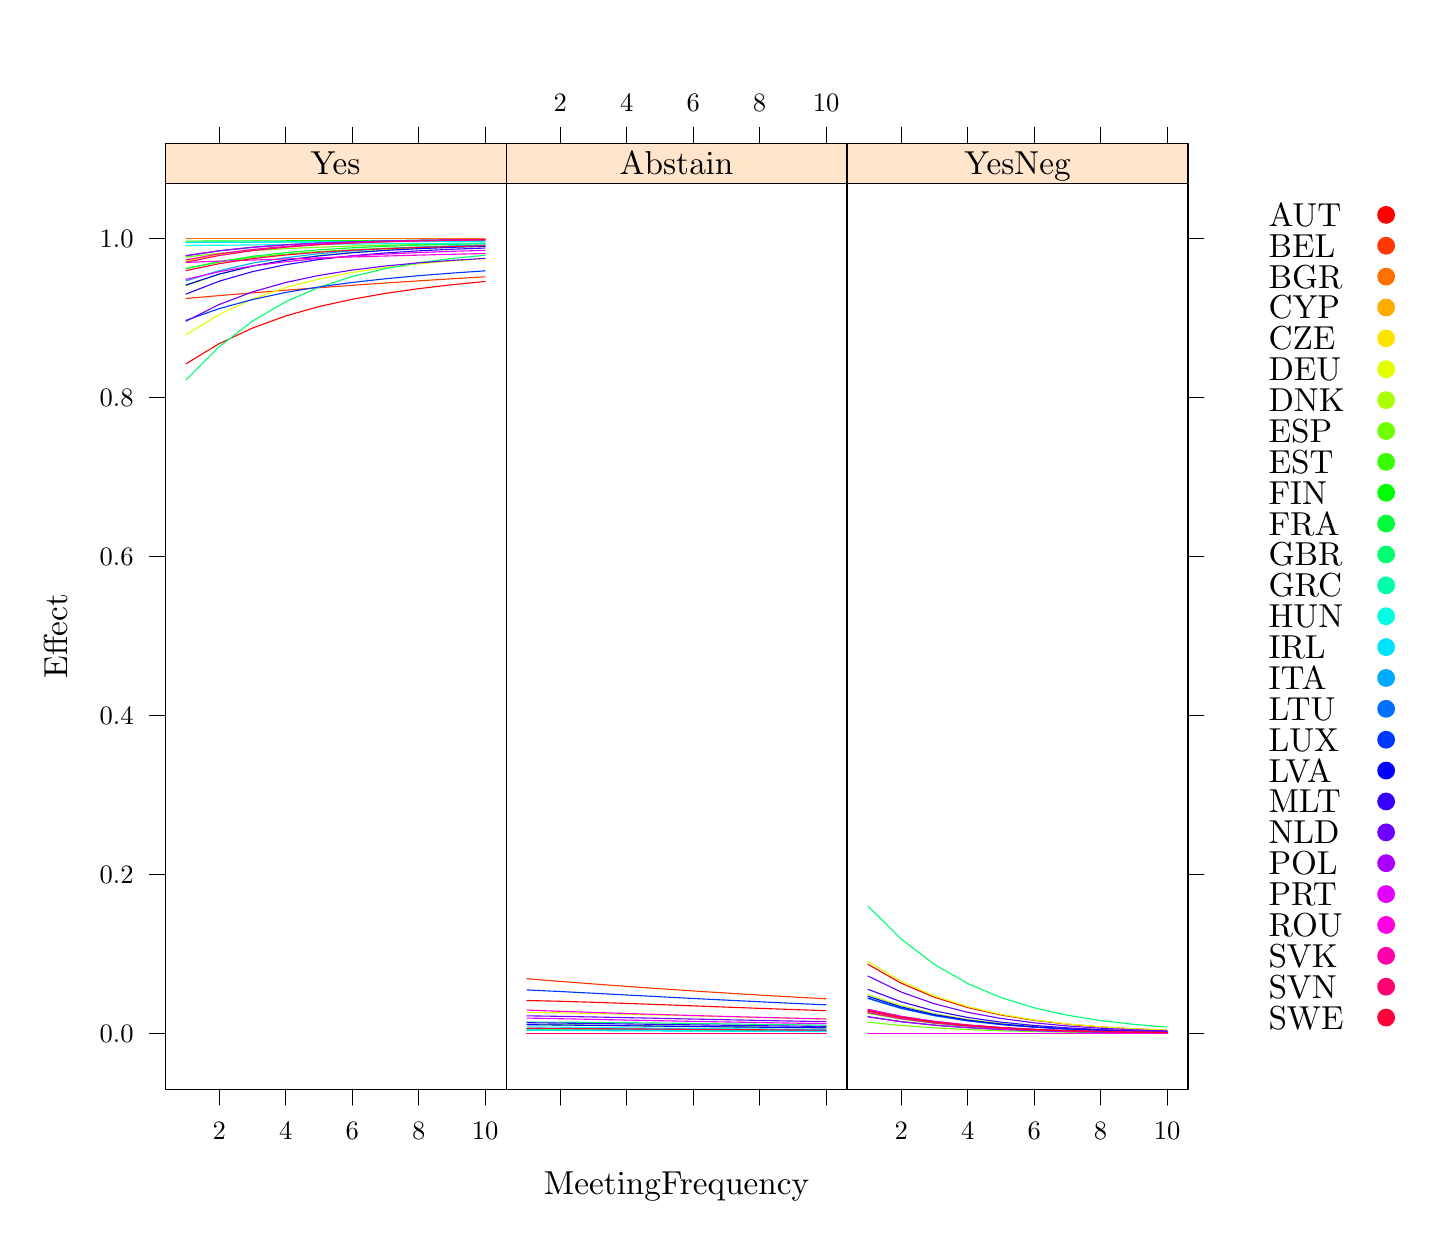
\begin{tikzpicture}[x=1pt,y=1pt]
\definecolor[named]{drawColor}{rgb}{0.00,0.00,0.00}
\definecolor[named]{fillColor}{rgb}{1.00,1.00,1.00}
\fill[color=fillColor,] (0,0) rectangle (505.89,433.62);
\begin{scope}
\path[clip] (  0.00,  0.00) rectangle (505.89,433.62);
\definecolor[named]{fillColor}{rgb}{0.00,0.00,0.00}
\end{scope}
\begin{scope}
\path[clip] (  0.00,  0.00) rectangle (505.89,433.62);
\definecolor[named]{fillColor}{rgb}{0.00,0.00,0.00}

\draw[fill opacity=0.00,draw opacity=0.00,] (  0.00,  0.00) rectangle (505.89,433.62);
\end{scope}
\begin{scope}
\path[clip] (  0.00,  0.00) rectangle (505.89,433.62);
\definecolor[named]{fillColor}{rgb}{0.00,0.00,0.00}
\end{scope}
\begin{scope}
\path[clip] (  0.00,  0.00) rectangle (505.89,433.62);
\definecolor[named]{fillColor}{rgb}{0.00,0.00,0.00}
\definecolor[named]{drawColor}{rgb}{0.00,0.00,0.00}

\node[color=drawColor,anchor=base,inner sep=0pt, outer sep=0pt, scale=  1.20] at (234.47, 12.04) {MeetingFrequency%
};
\end{scope}
\begin{scope}
\path[clip] (  0.00,  0.00) rectangle (505.89,433.62);
\definecolor[named]{fillColor}{rgb}{0.00,0.00,0.00}
\definecolor[named]{drawColor}{rgb}{0.00,0.00,0.00}

\node[rotate= 90.00,color=drawColor,anchor=base,inner sep=0pt, outer sep=0pt, scale=  1.20] at ( 14.29,213.72) {Effect%
};
\end{scope}
\begin{scope}
\path[clip] (  0.00,  0.00) rectangle (505.89,433.62);
\definecolor[named]{fillColor}{rgb}{0.00,0.00,0.00}
\end{scope}
\begin{scope}
\path[clip] (  0.00,  0.00) rectangle (505.89,433.62);
\definecolor[named]{fillColor}{rgb}{0.00,0.00,0.00}
\end{scope}
\begin{scope}
\path[clip] (  0.00,  0.00) rectangle (505.89,433.62);
\definecolor[named]{fillColor}{rgb}{0.00,0.00,0.00}
\end{scope}
\begin{scope}
\path[clip] ( 49.65, 50.02) rectangle (172.86,377.42);
\definecolor[named]{fillColor}{rgb}{0.00,0.00,0.00}
\end{scope}
\begin{scope}
\path[clip] (  0.00,  0.00) rectangle (505.89,433.62);
\definecolor[named]{fillColor}{rgb}{0.00,0.00,0.00}
\end{scope}
\begin{scope}
\path[clip] (  0.00,  0.00) rectangle (505.89,433.62);
\definecolor[named]{fillColor}{rgb}{0.00,0.00,0.00}
\definecolor[named]{drawColor}{rgb}{0.00,0.00,0.00}

\draw[color=drawColor,line cap=round,line join=round,fill opacity=0.00,] ( 69.22,391.87) -- ( 69.22,397.56);

\draw[color=drawColor,line cap=round,line join=round,fill opacity=0.00,] ( 93.24,391.87) -- ( 93.24,397.56);

\draw[color=drawColor,line cap=round,line join=round,fill opacity=0.00,] (117.26,391.87) -- (117.26,397.56);

\draw[color=drawColor,line cap=round,line join=round,fill opacity=0.00,] (141.28,391.87) -- (141.28,397.56);

\draw[color=drawColor,line cap=round,line join=round,fill opacity=0.00,] (165.29,391.87) -- (165.29,397.56);
\end{scope}
\begin{scope}
\path[clip] (  0.00,  0.00) rectangle (505.89,433.62);
\definecolor[named]{fillColor}{rgb}{0.00,0.00,0.00}
\end{scope}
\begin{scope}
\path[clip] (  0.00,  0.00) rectangle (505.89,433.62);
\definecolor[named]{fillColor}{rgb}{0.00,0.00,0.00}
\definecolor[named]{drawColor}{rgb}{0.00,0.00,0.00}

\draw[color=drawColor,line cap=round,line join=round,fill opacity=0.00,] ( 49.65, 70.12) -- ( 43.95, 70.12);

\draw[color=drawColor,line cap=round,line join=round,fill opacity=0.00,] ( 49.65,127.56) -- ( 43.95,127.56);

\draw[color=drawColor,line cap=round,line join=round,fill opacity=0.00,] ( 49.65,185.00) -- ( 43.95,185.00);

\draw[color=drawColor,line cap=round,line join=round,fill opacity=0.00,] ( 49.65,242.43) -- ( 43.95,242.43);

\draw[color=drawColor,line cap=round,line join=round,fill opacity=0.00,] ( 49.65,299.87) -- ( 43.95,299.87);

\draw[color=drawColor,line cap=round,line join=round,fill opacity=0.00,] ( 49.65,357.31) -- ( 43.95,357.31);

\node[color=drawColor,anchor=base east,inner sep=0pt, outer sep=0pt, scale=  0.96] at ( 38.26, 66.81) {0.0%
};

\node[color=drawColor,anchor=base east,inner sep=0pt, outer sep=0pt, scale=  0.96] at ( 38.26,124.25) {0.2%
};

\node[color=drawColor,anchor=base east,inner sep=0pt, outer sep=0pt, scale=  0.96] at ( 38.26,181.69) {0.4%
};

\node[color=drawColor,anchor=base east,inner sep=0pt, outer sep=0pt, scale=  0.96] at ( 38.26,239.13) {0.6%
};

\node[color=drawColor,anchor=base east,inner sep=0pt, outer sep=0pt, scale=  0.96] at ( 38.26,296.57) {0.8%
};

\node[color=drawColor,anchor=base east,inner sep=0pt, outer sep=0pt, scale=  0.96] at ( 38.26,354.01) {1.0%
};
\end{scope}
\begin{scope}
\path[clip] (  0.00,  0.00) rectangle (505.89,433.62);
\definecolor[named]{fillColor}{rgb}{0.00,0.00,0.00}
\end{scope}
\begin{scope}
\path[clip] (  0.00,  0.00) rectangle (505.89,433.62);
\definecolor[named]{fillColor}{rgb}{0.00,0.00,0.00}
\definecolor[named]{drawColor}{rgb}{0.00,0.00,0.00}

\draw[color=drawColor,line cap=round,line join=round,fill opacity=0.00,] ( 69.22, 50.02) -- ( 69.22, 44.32);

\draw[color=drawColor,line cap=round,line join=round,fill opacity=0.00,] ( 93.24, 50.02) -- ( 93.24, 44.32);

\draw[color=drawColor,line cap=round,line join=round,fill opacity=0.00,] (117.26, 50.02) -- (117.26, 44.32);

\draw[color=drawColor,line cap=round,line join=round,fill opacity=0.00,] (141.28, 50.02) -- (141.28, 44.32);

\draw[color=drawColor,line cap=round,line join=round,fill opacity=0.00,] (165.29, 50.02) -- (165.29, 44.32);

\node[color=drawColor,anchor=base,inner sep=0pt, outer sep=0pt, scale=  0.96] at ( 69.22, 32.02) {2%
};

\node[color=drawColor,anchor=base,inner sep=0pt, outer sep=0pt, scale=  0.96] at ( 93.24, 32.02) {4%
};

\node[color=drawColor,anchor=base,inner sep=0pt, outer sep=0pt, scale=  0.96] at (117.26, 32.02) {6%
};

\node[color=drawColor,anchor=base,inner sep=0pt, outer sep=0pt, scale=  0.96] at (141.28, 32.02) {8%
};

\node[color=drawColor,anchor=base,inner sep=0pt, outer sep=0pt, scale=  0.96] at (165.29, 32.02) {10%
};
\end{scope}
\begin{scope}
\path[clip] (  0.00,  0.00) rectangle (505.89,433.62);
\definecolor[named]{fillColor}{rgb}{0.00,0.00,0.00}
\end{scope}
\begin{scope}
\path[clip] ( 49.65, 50.02) rectangle (172.86,377.42);
\definecolor[named]{fillColor}{rgb}{0.00,0.00,0.00}
\definecolor[named]{drawColor}{rgb}{1.00,0.00,0.00}

\draw[color=drawColor,line cap=round,line join=round,fill opacity=0.00,] ( 57.21,312.15) --
	( 69.22,319.44) --
	( 81.23,325.08) --
	( 93.24,329.44) --
	(105.25,332.83) --
	(117.26,335.48) --
	(129.27,337.60) --
	(141.28,339.31) --
	(153.28,340.72) --
	(165.29,341.91);
\definecolor[named]{drawColor}{rgb}{1.00,0.22,0.00}

\draw[color=drawColor,line cap=round,line join=round,fill opacity=0.00,] ( 57.21,335.76) --
	( 69.22,336.80) --
	( 81.23,337.79) --
	( 93.24,338.74) --
	(105.25,339.65) --
	(117.26,340.52) --
	(129.27,341.34) --
	(141.28,342.13) --
	(153.28,342.88) --
	(165.29,343.59);
\definecolor[named]{drawColor}{rgb}{1.00,0.44,0.00}

\draw[color=drawColor,line cap=round,line join=round,fill opacity=0.00,] ( 57.21,357.31) --
	( 69.22,357.31) --
	( 81.23,357.31) --
	( 93.24,357.31) --
	(105.25,357.31) --
	(117.26,357.31) --
	(129.27,357.31) --
	(141.28,357.31) --
	(153.28,357.31) --
	(165.29,357.31);
\definecolor[named]{drawColor}{rgb}{1.00,0.67,0.00}

\draw[color=drawColor,line cap=round,line join=round,fill opacity=0.00,] ( 57.21,351.26) --
	( 69.22,353.01) --
	( 81.23,354.27) --
	( 93.24,355.16) --
	(105.25,355.79) --
	(117.26,356.23) --
	(129.27,356.55) --
	(141.28,356.77) --
	(153.28,356.93) --
	(165.29,357.04);
\definecolor[named]{drawColor}{rgb}{1.00,0.89,0.00}

\draw[color=drawColor,line cap=round,line join=round,fill opacity=0.00,] ( 57.21,349.29) --
	( 69.22,351.61) --
	( 81.23,353.26) --
	( 93.24,354.44) --
	(105.25,355.28) --
	(117.26,355.88) --
	(129.27,356.30) --
	(141.28,356.60) --
	(153.28,356.81) --
	(165.29,356.96);
\definecolor[named]{drawColor}{rgb}{0.89,1.00,0.00}

\draw[color=drawColor,line cap=round,line join=round,fill opacity=0.00,] ( 57.21,322.65) --
	( 69.22,329.99) --
	( 81.23,335.54) --
	( 93.24,339.70) --
	(105.25,342.81) --
	(117.26,345.15) --
	(129.27,346.91) --
	(141.28,348.26) --
	(153.28,349.31) --
	(165.29,350.13);
\definecolor[named]{drawColor}{rgb}{0.67,1.00,0.00}

\draw[color=drawColor,line cap=round,line join=round,fill opacity=0.00,] ( 57.21,340.40) --
	( 69.22,344.49) --
	( 81.23,347.49) --
	( 93.24,349.68) --
	(105.25,351.27) --
	(117.26,352.44) --
	(129.27,353.29) --
	(141.28,353.92) --
	(153.28,354.40) --
	(165.29,354.76);
\definecolor[named]{drawColor}{rgb}{0.44,1.00,0.00}

\draw[color=drawColor,line cap=round,line join=round,fill opacity=0.00,] ( 57.21,350.75) --
	( 69.22,352.08) --
	( 81.23,353.04) --
	( 93.24,353.76) --
	(105.25,354.29) --
	(117.26,354.70) --
	(129.27,355.00) --
	(141.28,355.25) --
	(153.28,355.44) --
	(165.29,355.59);
\definecolor[named]{drawColor}{rgb}{0.22,1.00,0.00}

\draw[color=drawColor,line cap=round,line join=round,fill opacity=0.00,] ( 57.21,346.60) --
	( 69.22,348.87) --
	( 81.23,350.54) --
	( 93.24,351.78) --
	(105.25,352.69) --
	(117.26,353.37) --
	(129.27,353.89) --
	(141.28,354.29) --
	(153.28,354.61) --
	(165.29,354.86);
\definecolor[named]{drawColor}{rgb}{0.00,1.00,0.00}

\draw[color=drawColor,line cap=round,line join=round,fill opacity=0.00,] ( 57.21,356.49) --
	( 69.22,356.53) --
	( 81.23,356.57) --
	( 93.24,356.60) --
	(105.25,356.64) --
	(117.26,356.67) --
	(129.27,356.70) --
	(141.28,356.73) --
	(153.28,356.76) --
	(165.29,356.78);
\definecolor[named]{drawColor}{rgb}{0.00,1.00,0.22}

\draw[color=drawColor,line cap=round,line join=round,fill opacity=0.00,] ( 57.21,346.52) --
	( 69.22,349.10) --
	( 81.23,350.98) --
	( 93.24,352.35) --
	(105.25,353.34) --
	(117.26,354.07) --
	(129.27,354.61) --
	(141.28,355.02) --
	(153.28,355.32) --
	(165.29,355.56);
\definecolor[named]{drawColor}{rgb}{0.00,1.00,0.44}

\draw[color=drawColor,line cap=round,line join=round,fill opacity=0.00,] ( 57.21,306.38) --
	( 69.22,318.33) --
	( 81.23,327.57) --
	( 93.24,334.58) --
	(105.25,339.81) --
	(117.26,343.69) --
	(129.27,346.55) --
	(141.28,348.66) --
	(153.28,350.21) --
	(165.29,351.37);
\definecolor[named]{drawColor}{rgb}{0.00,1.00,0.67}

\draw[color=drawColor,line cap=round,line join=round,fill opacity=0.00,] ( 57.21,355.94) --
	( 69.22,356.01) --
	( 81.23,356.08) --
	( 93.24,356.14) --
	(105.25,356.20) --
	(117.26,356.26) --
	(129.27,356.31) --
	(141.28,356.36) --
	(153.28,356.41) --
	(165.29,356.46);
\definecolor[named]{drawColor}{rgb}{0.00,1.00,0.89}

\draw[color=drawColor,line cap=round,line join=round,fill opacity=0.00,] ( 57.21,354.86) --
	( 69.22,354.99) --
	( 81.23,355.11) --
	( 93.24,355.22) --
	(105.25,355.33) --
	(117.26,355.43) --
	(129.27,355.53) --
	(141.28,355.63) --
	(153.28,355.71) --
	(165.29,355.80);
\definecolor[named]{drawColor}{rgb}{0.00,0.89,1.00}

\draw[color=drawColor,line cap=round,line join=round,fill opacity=0.00,] ( 57.21,355.99) --
	( 69.22,356.06) --
	( 81.23,356.13) --
	( 93.24,356.19) --
	(105.25,356.25) --
	(117.26,356.30) --
	(129.27,356.36) --
	(141.28,356.41) --
	(153.28,356.45) --
	(165.29,356.50);
\definecolor[named]{drawColor}{rgb}{0.00,0.67,1.00}

\draw[color=drawColor,line cap=round,line join=round,fill opacity=0.00,] ( 57.21,342.12) --
	( 69.22,345.82) --
	( 81.23,348.53) --
	( 93.24,350.50) --
	(105.25,351.93) --
	(117.26,352.98) --
	(129.27,353.75) --
	(141.28,354.33) --
	(153.28,354.75) --
	(165.29,355.08);
\definecolor[named]{drawColor}{rgb}{0.00,0.44,1.00}

\draw[color=drawColor,line cap=round,line join=round,fill opacity=0.00,] ( 57.21,351.18) --
	( 69.22,352.96) --
	( 81.23,354.23) --
	( 93.24,355.13) --
	(105.25,355.77) --
	(117.26,356.22) --
	(129.27,356.54) --
	(141.28,356.77) --
	(153.28,356.93) --
	(165.29,357.04);
\definecolor[named]{drawColor}{rgb}{0.00,0.22,1.00}

\draw[color=drawColor,line cap=round,line join=round,fill opacity=0.00,] ( 57.21,327.87) --
	( 69.22,332.10) --
	( 81.23,335.38) --
	( 93.24,337.93) --
	(105.25,339.94) --
	(117.26,341.56) --
	(129.27,342.88) --
	(141.28,343.99) --
	(153.28,344.93) --
	(165.29,345.74);
\definecolor[named]{drawColor}{rgb}{0.00,0.00,1.00}

\draw[color=drawColor,line cap=round,line join=round,fill opacity=0.00,] ( 57.21,340.63) --
	( 69.22,344.58) --
	( 81.23,347.47) --
	( 93.24,349.59) --
	(105.25,351.14) --
	(117.26,352.29) --
	(129.27,353.13) --
	(141.28,353.76) --
	(153.28,354.24) --
	(165.29,354.61);
\definecolor[named]{drawColor}{rgb}{0.22,0.00,1.00}

\draw[color=drawColor,line cap=round,line join=round,fill opacity=0.00,] ( 57.21,337.35) --
	( 69.22,342.01) --
	( 81.23,345.45) --
	( 93.24,347.97) --
	(105.25,349.83) --
	(117.26,351.20) --
	(129.27,352.21) --
	(141.28,352.97) --
	(153.28,353.55) --
	(165.29,353.99);
\definecolor[named]{drawColor}{rgb}{0.44,0.00,1.00}

\draw[color=drawColor,line cap=round,line join=round,fill opacity=0.00,] ( 57.21,327.55) --
	( 69.22,333.59) --
	( 81.23,338.13) --
	( 93.24,341.54) --
	(105.25,344.09) --
	(117.26,346.02) --
	(129.27,347.50) --
	(141.28,348.63) --
	(153.28,349.53) --
	(165.29,350.24);
\definecolor[named]{drawColor}{rgb}{0.67,0.00,1.00}

\draw[color=drawColor,line cap=round,line join=round,fill opacity=0.00,] ( 57.21,351.26) --
	( 69.22,353.02) --
	( 81.23,354.27) --
	( 93.24,355.16) --
	(105.25,355.79) --
	(117.26,356.24) --
	(129.27,356.55) --
	(141.28,356.78) --
	(153.28,356.93) --
	(165.29,357.04);
\definecolor[named]{drawColor}{rgb}{0.89,0.00,1.00}

\draw[color=drawColor,line cap=round,line join=round,fill opacity=0.00,] ( 57.21,342.67) --
	( 69.22,345.44) --
	( 81.23,347.51) --
	( 93.24,349.05) --
	(105.25,350.22) --
	(117.26,351.11) --
	(129.27,351.80) --
	(141.28,352.35) --
	(153.28,352.80) --
	(165.29,353.16);
\definecolor[named]{drawColor}{rgb}{1.00,0.00,0.89}

\draw[color=drawColor,line cap=round,line join=round,fill opacity=0.00,] ( 57.21,348.81) --
	( 69.22,349.24) --
	( 81.23,349.65) --
	( 93.24,350.04) --
	(105.25,350.41) --
	(117.26,350.77) --
	(129.27,351.10) --
	(141.28,351.42) --
	(153.28,351.73) --
	(165.29,352.01);
\definecolor[named]{drawColor}{rgb}{1.00,0.00,0.67}

\draw[color=drawColor,line cap=round,line join=round,fill opacity=0.00,] ( 57.21,349.70) --
	( 69.22,351.90) --
	( 81.23,353.47) --
	( 93.24,354.59) --
	(105.25,355.39) --
	(117.26,355.95) --
	(129.27,356.35) --
	(141.28,356.63) --
	(153.28,356.83) --
	(165.29,356.97);
\definecolor[named]{drawColor}{rgb}{1.00,0.00,0.44}

\draw[color=drawColor,line cap=round,line join=round,fill opacity=0.00,] ( 57.21,348.85) --
	( 69.22,351.29) --
	( 81.23,353.04) --
	( 93.24,354.28) --
	(105.25,355.17) --
	(117.26,355.80) --
	(129.27,356.24) --
	(141.28,356.56) --
	(153.28,356.78) --
	(165.29,356.93);
\definecolor[named]{drawColor}{rgb}{1.00,0.00,0.22}

\draw[color=drawColor,line cap=round,line join=round,fill opacity=0.00,] ( 57.21,345.85) --
	( 69.22,348.33) --
	( 81.23,350.15) --
	( 93.24,351.48) --
	(105.25,352.47) --
	(117.26,353.21) --
	(129.27,353.76) --
	(141.28,354.19) --
	(153.28,354.52) --
	(165.29,354.78);
\end{scope}
\begin{scope}
\path[clip] (  0.00,  0.00) rectangle (505.89,433.62);
\definecolor[named]{fillColor}{rgb}{0.00,0.00,0.00}
\end{scope}
\begin{scope}
\path[clip] (  0.00,  0.00) rectangle (505.89,433.62);
\definecolor[named]{fillColor}{rgb}{0.00,0.00,0.00}
\definecolor[named]{drawColor}{rgb}{0.00,0.00,0.00}

\draw[color=drawColor,line cap=round,line join=round,fill opacity=0.00,] ( 49.65, 50.02) rectangle (172.86,377.42);
\end{scope}
\begin{scope}
\path[clip] (  0.00,  0.00) rectangle (505.89,433.62);
\definecolor[named]{fillColor}{rgb}{0.00,0.00,0.00}
\end{scope}
\begin{scope}
\path[clip] (  0.00,  0.00) rectangle (505.89,433.62);
\definecolor[named]{fillColor}{rgb}{0.00,0.00,0.00}
\end{scope}
\begin{scope}
\path[clip] ( 49.65,377.42) rectangle (172.86,391.87);
\definecolor[named]{fillColor}{rgb}{0.00,0.00,0.00}
\definecolor[named]{drawColor}{rgb}{1.00,0.90,0.80}
\definecolor[named]{fillColor}{rgb}{1.00,0.90,0.80}

\draw[color=drawColor,line cap=round,line join=round,fill=fillColor,] ( 49.65,377.42) rectangle (172.86,391.87);
\definecolor[named]{drawColor}{rgb}{0.00,0.00,0.00}

\node[color=drawColor,anchor=base west,inner sep=0pt, outer sep=0pt, scale=  1.20] at (102.22,380.51) {Yes%
};
\end{scope}
\begin{scope}
\path[clip] (  0.00,  0.00) rectangle (505.89,433.62);
\definecolor[named]{fillColor}{rgb}{0.00,0.00,0.00}
\end{scope}
\begin{scope}
\path[clip] (  0.00,  0.00) rectangle (505.89,433.62);
\definecolor[named]{fillColor}{rgb}{0.00,0.00,0.00}
\definecolor[named]{drawColor}{rgb}{0.00,0.00,0.00}

\draw[color=drawColor,line cap=round,line join=round,fill opacity=0.00,] ( 49.65,377.42) rectangle (172.86,391.87);
\end{scope}
\begin{scope}
\path[clip] (  0.00,  0.00) rectangle (505.89,433.62);
\definecolor[named]{fillColor}{rgb}{0.00,0.00,0.00}
\end{scope}
\begin{scope}
\path[clip] (  0.00,  0.00) rectangle (505.89,433.62);
\definecolor[named]{fillColor}{rgb}{0.00,0.00,0.00}
\end{scope}
\begin{scope}
\path[clip] (172.86, 50.02) rectangle (296.07,377.42);
\definecolor[named]{fillColor}{rgb}{0.00,0.00,0.00}
\end{scope}
\begin{scope}
\path[clip] (  0.00,  0.00) rectangle (505.89,433.62);
\definecolor[named]{fillColor}{rgb}{0.00,0.00,0.00}
\end{scope}
\begin{scope}
\path[clip] (  0.00,  0.00) rectangle (505.89,433.62);
\definecolor[named]{fillColor}{rgb}{0.00,0.00,0.00}
\definecolor[named]{drawColor}{rgb}{0.00,0.00,0.00}

\draw[color=drawColor,line cap=round,line join=round,fill opacity=0.00,] (192.43,391.87) -- (192.43,397.56);

\draw[color=drawColor,line cap=round,line join=round,fill opacity=0.00,] (216.45,391.87) -- (216.45,397.56);

\draw[color=drawColor,line cap=round,line join=round,fill opacity=0.00,] (240.47,391.87) -- (240.47,397.56);

\draw[color=drawColor,line cap=round,line join=round,fill opacity=0.00,] (264.49,391.87) -- (264.49,397.56);

\draw[color=drawColor,line cap=round,line join=round,fill opacity=0.00,] (288.51,391.87) -- (288.51,397.56);

\node[color=drawColor,anchor=base,inner sep=0pt, outer sep=0pt, scale=  0.96] at (192.43,403.25) {2%
};

\node[color=drawColor,anchor=base,inner sep=0pt, outer sep=0pt, scale=  0.96] at (216.45,403.25) {4%
};

\node[color=drawColor,anchor=base,inner sep=0pt, outer sep=0pt, scale=  0.96] at (240.47,403.25) {6%
};

\node[color=drawColor,anchor=base,inner sep=0pt, outer sep=0pt, scale=  0.96] at (264.49,403.25) {8%
};

\node[color=drawColor,anchor=base,inner sep=0pt, outer sep=0pt, scale=  0.96] at (288.51,403.25) {10%
};
\end{scope}
\begin{scope}
\path[clip] (  0.00,  0.00) rectangle (505.89,433.62);
\definecolor[named]{fillColor}{rgb}{0.00,0.00,0.00}
\end{scope}
\begin{scope}
\path[clip] (  0.00,  0.00) rectangle (505.89,433.62);
\definecolor[named]{fillColor}{rgb}{0.00,0.00,0.00}
\end{scope}
\begin{scope}
\path[clip] (  0.00,  0.00) rectangle (505.89,433.62);
\definecolor[named]{fillColor}{rgb}{0.00,0.00,0.00}
\end{scope}
\begin{scope}
\path[clip] (  0.00,  0.00) rectangle (505.89,433.62);
\definecolor[named]{fillColor}{rgb}{0.00,0.00,0.00}
\definecolor[named]{drawColor}{rgb}{0.00,0.00,0.00}

\draw[color=drawColor,line cap=round,line join=round,fill opacity=0.00,] (192.43, 50.02) -- (192.43, 44.32);

\draw[color=drawColor,line cap=round,line join=round,fill opacity=0.00,] (216.45, 50.02) -- (216.45, 44.32);

\draw[color=drawColor,line cap=round,line join=round,fill opacity=0.00,] (240.47, 50.02) -- (240.47, 44.32);

\draw[color=drawColor,line cap=round,line join=round,fill opacity=0.00,] (264.49, 50.02) -- (264.49, 44.32);

\draw[color=drawColor,line cap=round,line join=round,fill opacity=0.00,] (288.51, 50.02) -- (288.51, 44.32);
\end{scope}
\begin{scope}
\path[clip] (  0.00,  0.00) rectangle (505.89,433.62);
\definecolor[named]{fillColor}{rgb}{0.00,0.00,0.00}
\end{scope}
\begin{scope}
\path[clip] (172.86, 50.02) rectangle (296.07,377.42);
\definecolor[named]{fillColor}{rgb}{0.00,0.00,0.00}
\definecolor[named]{drawColor}{rgb}{1.00,0.00,0.00}

\draw[color=drawColor,line cap=round,line join=round,fill opacity=0.00,] (180.42, 82.09) --
	(192.43, 81.81) --
	(204.44, 81.44) --
	(216.45, 81.03) --
	(228.46, 80.60) --
	(240.47, 80.15) --
	(252.48, 79.70) --
	(264.49, 79.25) --
	(276.50, 78.82) --
	(288.51, 78.40);
\definecolor[named]{drawColor}{rgb}{1.00,0.22,0.00}

\draw[color=drawColor,line cap=round,line join=round,fill opacity=0.00,] (180.42, 89.96) --
	(192.43, 88.99) --
	(204.44, 88.07) --
	(216.45, 87.19) --
	(228.46, 86.35) --
	(240.47, 85.54) --
	(252.48, 84.78) --
	(264.49, 84.05) --
	(276.50, 83.36) --
	(288.51, 82.70);
\definecolor[named]{drawColor}{rgb}{1.00,0.44,0.00}

\draw[color=drawColor,line cap=round,line join=round,fill opacity=0.00,] (180.42, 70.12) --
	(192.43, 70.12) --
	(204.44, 70.12) --
	(216.45, 70.12) --
	(228.46, 70.12) --
	(240.47, 70.12) --
	(252.48, 70.12) --
	(264.49, 70.12) --
	(276.50, 70.12) --
	(288.51, 70.12);
\definecolor[named]{drawColor}{rgb}{1.00,0.67,0.00}

\draw[color=drawColor,line cap=round,line join=round,fill opacity=0.00,] (180.42, 70.12) --
	(192.43, 70.12) --
	(204.44, 70.12) --
	(216.45, 70.12) --
	(228.46, 70.12) --
	(240.47, 70.12) --
	(252.48, 70.12) --
	(264.49, 70.12) --
	(276.50, 70.12) --
	(288.51, 70.12);
\definecolor[named]{drawColor}{rgb}{1.00,0.89,0.00}

\draw[color=drawColor,line cap=round,line join=round,fill opacity=0.00,] (180.42, 70.12) --
	(192.43, 70.12) --
	(204.44, 70.12) --
	(216.45, 70.12) --
	(228.46, 70.12) --
	(240.47, 70.12) --
	(252.48, 70.12) --
	(264.49, 70.12) --
	(276.50, 70.12) --
	(288.51, 70.12);
\definecolor[named]{drawColor}{rgb}{0.89,1.00,0.00}

\draw[color=drawColor,line cap=round,line join=round,fill opacity=0.00,] (180.42, 77.83) --
	(192.43, 77.64) --
	(204.44, 77.40) --
	(216.45, 77.12) --
	(228.46, 76.83) --
	(240.47, 76.54) --
	(252.48, 76.24) --
	(264.49, 75.95) --
	(276.50, 75.66) --
	(288.51, 75.39);
\definecolor[named]{drawColor}{rgb}{0.67,1.00,0.00}

\draw[color=drawColor,line cap=round,line join=round,fill opacity=0.00,] (180.42, 70.12) --
	(192.43, 70.12) --
	(204.44, 70.12) --
	(216.45, 70.12) --
	(228.46, 70.12) --
	(240.47, 70.12) --
	(252.48, 70.12) --
	(264.49, 70.12) --
	(276.50, 70.12) --
	(288.51, 70.12);
\definecolor[named]{drawColor}{rgb}{0.44,1.00,0.00}

\draw[color=drawColor,line cap=round,line join=round,fill opacity=0.00,] (180.42, 71.58) --
	(192.43, 71.51) --
	(204.44, 71.45) --
	(216.45, 71.38) --
	(228.46, 71.31) --
	(240.47, 71.25) --
	(252.48, 71.20) --
	(264.49, 71.14) --
	(276.50, 71.09) --
	(288.51, 71.04);
\definecolor[named]{drawColor}{rgb}{0.22,1.00,0.00}

\draw[color=drawColor,line cap=round,line join=round,fill opacity=0.00,] (180.42, 73.46) --
	(192.43, 73.32) --
	(204.44, 73.17) --
	(216.45, 73.02) --
	(228.46, 72.88) --
	(240.47, 72.74) --
	(252.48, 72.60) --
	(264.49, 72.48) --
	(276.50, 72.36) --
	(288.51, 72.24);
\definecolor[named]{drawColor}{rgb}{0.00,1.00,0.00}

\draw[color=drawColor,line cap=round,line join=round,fill opacity=0.00,] (180.42, 70.12) --
	(192.43, 70.12) --
	(204.44, 70.12) --
	(216.45, 70.12) --
	(228.46, 70.12) --
	(240.47, 70.12) --
	(252.48, 70.12) --
	(264.49, 70.12) --
	(276.50, 70.12) --
	(288.51, 70.12);
\definecolor[named]{drawColor}{rgb}{0.00,1.00,0.22}

\draw[color=drawColor,line cap=round,line join=round,fill opacity=0.00,] (180.42, 71.96) --
	(192.43, 71.88) --
	(204.44, 71.80) --
	(216.45, 71.72) --
	(228.46, 71.64) --
	(240.47, 71.56) --
	(252.48, 71.49) --
	(264.49, 71.42) --
	(276.50, 71.35) --
	(288.51, 71.29);
\definecolor[named]{drawColor}{rgb}{0.00,1.00,0.44}

\draw[color=drawColor,line cap=round,line join=round,fill opacity=0.00,] (180.42, 74.27) --
	(192.43, 74.25) --
	(204.44, 74.18) --
	(216.45, 74.07) --
	(228.46, 73.94) --
	(240.47, 73.79) --
	(252.48, 73.63) --
	(264.49, 73.47) --
	(276.50, 73.32) --
	(288.51, 73.16);
\definecolor[named]{drawColor}{rgb}{0.00,1.00,0.67}

\draw[color=drawColor,line cap=round,line join=round,fill opacity=0.00,] (180.42, 71.32) --
	(192.43, 71.26) --
	(204.44, 71.20) --
	(216.45, 71.14) --
	(228.46, 71.09) --
	(240.47, 71.04) --
	(252.48, 70.99) --
	(264.49, 70.94) --
	(276.50, 70.90) --
	(288.51, 70.86);
\definecolor[named]{drawColor}{rgb}{0.00,1.00,0.89}

\draw[color=drawColor,line cap=round,line join=round,fill opacity=0.00,] (180.42, 72.57) --
	(192.43, 72.44) --
	(204.44, 72.32) --
	(216.45, 72.21) --
	(228.46, 72.10) --
	(240.47, 72.00) --
	(252.48, 71.90) --
	(264.49, 71.81) --
	(276.50, 71.72) --
	(288.51, 71.63);
\definecolor[named]{drawColor}{rgb}{0.00,0.89,1.00}

\draw[color=drawColor,line cap=round,line join=round,fill opacity=0.00,] (180.42, 71.44) --
	(192.43, 71.37) --
	(204.44, 71.30) --
	(216.45, 71.24) --
	(228.46, 71.18) --
	(240.47, 71.13) --
	(252.48, 71.07) --
	(264.49, 71.02) --
	(276.50, 70.98) --
	(288.51, 70.93);
\definecolor[named]{drawColor}{rgb}{0.00,0.67,1.00}

\draw[color=drawColor,line cap=round,line join=round,fill opacity=0.00,] (180.42, 72.01) --
	(192.43, 71.93) --
	(204.44, 71.85) --
	(216.45, 71.77) --
	(228.46, 71.70) --
	(240.47, 71.62) --
	(252.48, 71.54) --
	(264.49, 71.47) --
	(276.50, 71.40) --
	(288.51, 71.34);
\definecolor[named]{drawColor}{rgb}{0.00,0.44,1.00}

\draw[color=drawColor,line cap=round,line join=round,fill opacity=0.00,] (180.42, 70.12) --
	(192.43, 70.12) --
	(204.44, 70.12) --
	(216.45, 70.12) --
	(228.46, 70.12) --
	(240.47, 70.12) --
	(252.48, 70.12) --
	(264.49, 70.12) --
	(276.50, 70.12) --
	(288.51, 70.12);
\definecolor[named]{drawColor}{rgb}{0.00,0.22,1.00}

\draw[color=drawColor,line cap=round,line join=round,fill opacity=0.00,] (180.42, 85.91) --
	(192.43, 85.33) --
	(204.44, 84.71) --
	(216.45, 84.08) --
	(228.46, 83.45) --
	(240.47, 82.82) --
	(252.48, 82.22) --
	(264.49, 81.63) --
	(276.50, 81.06) --
	(288.51, 80.52);
\definecolor[named]{drawColor}{rgb}{0.00,0.00,1.00}

\draw[color=drawColor,line cap=round,line join=round,fill opacity=0.00,] (180.42, 73.35) --
	(192.43, 73.22) --
	(204.44, 73.09) --
	(216.45, 72.96) --
	(228.46, 72.82) --
	(240.47, 72.69) --
	(252.48, 72.56) --
	(264.49, 72.44) --
	(276.50, 72.32) --
	(288.51, 72.21);
\definecolor[named]{drawColor}{rgb}{0.22,0.00,1.00}

\draw[color=drawColor,line cap=round,line join=round,fill opacity=0.00,] (180.42, 74.07) --
	(192.43, 73.92) --
	(204.44, 73.77) --
	(216.45, 73.61) --
	(228.46, 73.45) --
	(240.47, 73.29) --
	(252.48, 73.14) --
	(264.49, 72.98) --
	(276.50, 72.84) --
	(288.51, 72.70);
\definecolor[named]{drawColor}{rgb}{0.44,0.00,1.00}

\draw[color=drawColor,line cap=round,line join=round,fill opacity=0.00,] (180.42, 76.55) --
	(192.43, 76.36) --
	(204.44, 76.13) --
	(216.45, 75.89) --
	(228.46, 75.64) --
	(240.47, 75.38) --
	(252.48, 75.14) --
	(264.49, 74.89) --
	(276.50, 74.66) --
	(288.51, 74.43);
\definecolor[named]{drawColor}{rgb}{0.67,0.00,1.00}

\draw[color=drawColor,line cap=round,line join=round,fill opacity=0.00,] (180.42, 70.12) --
	(192.43, 70.12) --
	(204.44, 70.12) --
	(216.45, 70.12) --
	(228.46, 70.12) --
	(240.47, 70.12) --
	(252.48, 70.12) --
	(264.49, 70.12) --
	(276.50, 70.12) --
	(288.51, 70.12);
\definecolor[named]{drawColor}{rgb}{0.89,0.00,1.00}

\draw[color=drawColor,line cap=round,line join=round,fill opacity=0.00,] (180.42, 75.74) --
	(192.43, 75.50) --
	(204.44, 75.26) --
	(216.45, 75.02) --
	(228.46, 74.78) --
	(240.47, 74.55) --
	(252.48, 74.33) --
	(264.49, 74.11) --
	(276.50, 73.91) --
	(288.51, 73.72);
\definecolor[named]{drawColor}{rgb}{1.00,0.00,0.89}

\draw[color=drawColor,line cap=round,line join=round,fill opacity=0.00,] (180.42, 78.62) --
	(192.43, 78.19) --
	(204.44, 77.78) --
	(216.45, 77.39) --
	(228.46, 77.02) --
	(240.47, 76.66) --
	(252.48, 76.33) --
	(264.49, 76.01) --
	(276.50, 75.71) --
	(288.51, 75.42);
\definecolor[named]{drawColor}{rgb}{1.00,0.00,0.67}

\draw[color=drawColor,line cap=round,line join=round,fill opacity=0.00,] (180.42, 70.12) --
	(192.43, 70.12) --
	(204.44, 70.12) --
	(216.45, 70.12) --
	(228.46, 70.12) --
	(240.47, 70.12) --
	(252.48, 70.12) --
	(264.49, 70.12) --
	(276.50, 70.12) --
	(288.51, 70.12);
\definecolor[named]{drawColor}{rgb}{1.00,0.00,0.44}

\draw[color=drawColor,line cap=round,line join=round,fill opacity=0.00,] (180.42, 70.12) --
	(192.43, 70.12) --
	(204.44, 70.12) --
	(216.45, 70.12) --
	(228.46, 70.12) --
	(240.47, 70.12) --
	(252.48, 70.12) --
	(264.49, 70.12) --
	(276.50, 70.12) --
	(288.51, 70.12);
\definecolor[named]{drawColor}{rgb}{1.00,0.00,0.22}

\draw[color=drawColor,line cap=round,line join=round,fill opacity=0.00,] (180.42, 72.08) --
	(192.43, 72.00) --
	(204.44, 71.91) --
	(216.45, 71.82) --
	(228.46, 71.74) --
	(240.47, 71.66) --
	(252.48, 71.58) --
	(264.49, 71.51) --
	(276.50, 71.43) --
	(288.51, 71.37);
\end{scope}
\begin{scope}
\path[clip] (  0.00,  0.00) rectangle (505.89,433.62);
\definecolor[named]{fillColor}{rgb}{0.00,0.00,0.00}
\end{scope}
\begin{scope}
\path[clip] (  0.00,  0.00) rectangle (505.89,433.62);
\definecolor[named]{fillColor}{rgb}{0.00,0.00,0.00}
\definecolor[named]{drawColor}{rgb}{0.00,0.00,0.00}

\draw[color=drawColor,line cap=round,line join=round,fill opacity=0.00,] (172.86, 50.02) rectangle (296.07,377.42);
\end{scope}
\begin{scope}
\path[clip] (  0.00,  0.00) rectangle (505.89,433.62);
\definecolor[named]{fillColor}{rgb}{0.00,0.00,0.00}
\end{scope}
\begin{scope}
\path[clip] (  0.00,  0.00) rectangle (505.89,433.62);
\definecolor[named]{fillColor}{rgb}{0.00,0.00,0.00}
\end{scope}
\begin{scope}
\path[clip] (172.86,377.42) rectangle (296.07,391.87);
\definecolor[named]{fillColor}{rgb}{0.00,0.00,0.00}
\definecolor[named]{drawColor}{rgb}{1.00,0.90,0.80}
\definecolor[named]{fillColor}{rgb}{1.00,0.90,0.80}

\draw[color=drawColor,line cap=round,line join=round,fill=fillColor,] (172.86,377.42) rectangle (296.07,391.87);
\definecolor[named]{drawColor}{rgb}{0.00,0.00,0.00}

\node[color=drawColor,anchor=base west,inner sep=0pt, outer sep=0pt, scale=  1.20] at (213.94,380.51) {Abstain%
};
\end{scope}
\begin{scope}
\path[clip] (  0.00,  0.00) rectangle (505.89,433.62);
\definecolor[named]{fillColor}{rgb}{0.00,0.00,0.00}
\end{scope}
\begin{scope}
\path[clip] (  0.00,  0.00) rectangle (505.89,433.62);
\definecolor[named]{fillColor}{rgb}{0.00,0.00,0.00}
\definecolor[named]{drawColor}{rgb}{0.00,0.00,0.00}

\draw[color=drawColor,line cap=round,line join=round,fill opacity=0.00,] (172.86,377.42) rectangle (296.07,391.87);
\end{scope}
\begin{scope}
\path[clip] (  0.00,  0.00) rectangle (505.89,433.62);
\definecolor[named]{fillColor}{rgb}{0.00,0.00,0.00}
\end{scope}
\begin{scope}
\path[clip] (  0.00,  0.00) rectangle (505.89,433.62);
\definecolor[named]{fillColor}{rgb}{0.00,0.00,0.00}
\end{scope}
\begin{scope}
\path[clip] (296.07, 50.02) rectangle (419.29,377.42);
\definecolor[named]{fillColor}{rgb}{0.00,0.00,0.00}
\end{scope}
\begin{scope}
\path[clip] (  0.00,  0.00) rectangle (505.89,433.62);
\definecolor[named]{fillColor}{rgb}{0.00,0.00,0.00}
\end{scope}
\begin{scope}
\path[clip] (  0.00,  0.00) rectangle (505.89,433.62);
\definecolor[named]{fillColor}{rgb}{0.00,0.00,0.00}
\definecolor[named]{drawColor}{rgb}{0.00,0.00,0.00}

\draw[color=drawColor,line cap=round,line join=round,fill opacity=0.00,] (315.65,391.87) -- (315.65,397.56);

\draw[color=drawColor,line cap=round,line join=round,fill opacity=0.00,] (339.67,391.87) -- (339.67,397.56);

\draw[color=drawColor,line cap=round,line join=round,fill opacity=0.00,] (363.69,391.87) -- (363.69,397.56);

\draw[color=drawColor,line cap=round,line join=round,fill opacity=0.00,] (387.70,391.87) -- (387.70,397.56);

\draw[color=drawColor,line cap=round,line join=round,fill opacity=0.00,] (411.72,391.87) -- (411.72,397.56);
\end{scope}
\begin{scope}
\path[clip] (  0.00,  0.00) rectangle (505.89,433.62);
\definecolor[named]{fillColor}{rgb}{0.00,0.00,0.00}
\end{scope}
\begin{scope}
\path[clip] (  0.00,  0.00) rectangle (505.89,433.62);
\definecolor[named]{fillColor}{rgb}{0.00,0.00,0.00}
\end{scope}
\begin{scope}
\path[clip] (  0.00,  0.00) rectangle (505.89,433.62);
\definecolor[named]{fillColor}{rgb}{0.00,0.00,0.00}
\end{scope}
\begin{scope}
\path[clip] (  0.00,  0.00) rectangle (505.89,433.62);
\definecolor[named]{fillColor}{rgb}{0.00,0.00,0.00}
\definecolor[named]{drawColor}{rgb}{0.00,0.00,0.00}

\draw[color=drawColor,line cap=round,line join=round,fill opacity=0.00,] (315.65, 50.02) -- (315.65, 44.32);

\draw[color=drawColor,line cap=round,line join=round,fill opacity=0.00,] (339.67, 50.02) -- (339.67, 44.32);

\draw[color=drawColor,line cap=round,line join=round,fill opacity=0.00,] (363.69, 50.02) -- (363.69, 44.32);

\draw[color=drawColor,line cap=round,line join=round,fill opacity=0.00,] (387.70, 50.02) -- (387.70, 44.32);

\draw[color=drawColor,line cap=round,line join=round,fill opacity=0.00,] (411.72, 50.02) -- (411.72, 44.32);

\node[color=drawColor,anchor=base,inner sep=0pt, outer sep=0pt, scale=  0.96] at (315.65, 32.02) {2%
};

\node[color=drawColor,anchor=base,inner sep=0pt, outer sep=0pt, scale=  0.96] at (339.67, 32.02) {4%
};

\node[color=drawColor,anchor=base,inner sep=0pt, outer sep=0pt, scale=  0.96] at (363.69, 32.02) {6%
};

\node[color=drawColor,anchor=base,inner sep=0pt, outer sep=0pt, scale=  0.96] at (387.70, 32.02) {8%
};

\node[color=drawColor,anchor=base,inner sep=0pt, outer sep=0pt, scale=  0.96] at (411.72, 32.02) {10%
};

\draw[color=drawColor,line cap=round,line join=round,fill opacity=0.00,] (419.29, 70.12) -- (424.98, 70.12);

\draw[color=drawColor,line cap=round,line join=round,fill opacity=0.00,] (419.29,127.56) -- (424.98,127.56);

\draw[color=drawColor,line cap=round,line join=round,fill opacity=0.00,] (419.29,185.00) -- (424.98,185.00);

\draw[color=drawColor,line cap=round,line join=round,fill opacity=0.00,] (419.29,242.43) -- (424.98,242.43);

\draw[color=drawColor,line cap=round,line join=round,fill opacity=0.00,] (419.29,299.87) -- (424.98,299.87);

\draw[color=drawColor,line cap=round,line join=round,fill opacity=0.00,] (419.29,357.31) -- (424.98,357.31);
\end{scope}
\begin{scope}
\path[clip] (  0.00,  0.00) rectangle (505.89,433.62);
\definecolor[named]{fillColor}{rgb}{0.00,0.00,0.00}
\end{scope}
\begin{scope}
\path[clip] (296.07, 50.02) rectangle (419.29,377.42);
\definecolor[named]{fillColor}{rgb}{0.00,0.00,0.00}
\definecolor[named]{drawColor}{rgb}{1.00,0.00,0.00}

\draw[color=drawColor,line cap=round,line join=round,fill opacity=0.00,] (303.64, 95.17) --
	(315.65, 88.33) --
	(327.66, 83.25) --
	(339.67, 79.54) --
	(351.68, 76.85) --
	(363.69, 74.92) --
	(375.69, 73.53) --
	(387.70, 72.54) --
	(399.71, 71.84) --
	(411.72, 71.34);
\definecolor[named]{drawColor}{rgb}{1.00,0.22,0.00}

\draw[color=drawColor,line cap=round,line join=round,fill opacity=0.00,] (303.64, 70.12) --
	(315.65, 70.12) --
	(327.66, 70.12) --
	(339.67, 70.12) --
	(351.68, 70.12) --
	(363.69, 70.12) --
	(375.69, 70.12) --
	(387.70, 70.12) --
	(399.71, 70.12) --
	(411.72, 70.12);
\definecolor[named]{drawColor}{rgb}{1.00,0.44,0.00}

\draw[color=drawColor,line cap=round,line join=round,fill opacity=0.00,] (303.64, 70.12) --
	(315.65, 70.12) --
	(327.66, 70.12) --
	(339.67, 70.12) --
	(351.68, 70.12) --
	(363.69, 70.12) --
	(375.69, 70.12) --
	(387.70, 70.12) --
	(399.71, 70.12) --
	(411.72, 70.12);
\definecolor[named]{drawColor}{rgb}{1.00,0.67,0.00}

\draw[color=drawColor,line cap=round,line join=round,fill opacity=0.00,] (303.64, 76.17) --
	(315.65, 74.42) --
	(327.66, 73.17) --
	(339.67, 72.27) --
	(351.68, 71.64) --
	(363.69, 71.20) --
	(375.69, 70.88) --
	(387.70, 70.66) --
	(399.71, 70.50) --
	(411.72, 70.39);
\definecolor[named]{drawColor}{rgb}{1.00,0.89,0.00}

\draw[color=drawColor,line cap=round,line join=round,fill opacity=0.00,] (303.64, 78.14) --
	(315.65, 75.82) --
	(327.66, 74.17) --
	(339.67, 72.99) --
	(351.68, 72.15) --
	(363.69, 71.55) --
	(375.69, 71.13) --
	(387.70, 70.83) --
	(399.71, 70.62) --
	(411.72, 70.48);
\definecolor[named]{drawColor}{rgb}{0.89,1.00,0.00}

\draw[color=drawColor,line cap=round,line join=round,fill opacity=0.00,] (303.64, 96.13) --
	(315.65, 89.00) --
	(327.66, 83.73) --
	(339.67, 79.87) --
	(351.68, 77.08) --
	(363.69, 75.07) --
	(375.69, 73.63) --
	(387.70, 72.61) --
	(399.71, 71.88) --
	(411.72, 71.37);
\definecolor[named]{drawColor}{rgb}{0.67,1.00,0.00}

\draw[color=drawColor,line cap=round,line join=round,fill opacity=0.00,] (303.64, 84.22) --
	(315.65, 80.22) --
	(327.66, 77.32) --
	(339.67, 75.24) --
	(351.68, 73.75) --
	(363.69, 72.69) --
	(375.69, 71.94) --
	(387.70, 71.41) --
	(399.71, 71.03) --
	(411.72, 70.76);
\definecolor[named]{drawColor}{rgb}{0.44,1.00,0.00}

\draw[color=drawColor,line cap=round,line join=round,fill opacity=0.00,] (303.64, 74.27) --
	(315.65, 73.06) --
	(327.66, 72.20) --
	(339.67, 71.59) --
	(351.68, 71.16) --
	(363.69, 70.86) --
	(375.69, 70.64) --
	(387.70, 70.49) --
	(399.71, 70.38) --
	(411.72, 70.30);
\definecolor[named]{drawColor}{rgb}{0.22,1.00,0.00}

\draw[color=drawColor,line cap=round,line join=round,fill opacity=0.00,] (303.64, 77.49) --
	(315.65, 75.36) --
	(327.66, 73.84) --
	(339.67, 72.75) --
	(351.68, 71.98) --
	(363.69, 71.44) --
	(375.69, 71.05) --
	(387.70, 70.78) --
	(399.71, 70.58) --
	(411.72, 70.45);
\definecolor[named]{drawColor}{rgb}{0.00,1.00,0.00}

\draw[color=drawColor,line cap=round,line join=round,fill opacity=0.00,] (303.64, 70.12) --
	(315.65, 70.12) --
	(327.66, 70.12) --
	(339.67, 70.12) --
	(351.68, 70.12) --
	(363.69, 70.12) --
	(375.69, 70.12) --
	(387.70, 70.12) --
	(399.71, 70.12) --
	(411.72, 70.12);
\definecolor[named]{drawColor}{rgb}{0.00,1.00,0.22}

\draw[color=drawColor,line cap=round,line join=round,fill opacity=0.00,] (303.64, 78.77) --
	(315.65, 76.28) --
	(327.66, 74.49) --
	(339.67, 73.22) --
	(351.68, 72.31) --
	(363.69, 71.67) --
	(375.69, 71.22) --
	(387.70, 70.89) --
	(399.71, 70.67) --
	(411.72, 70.51);
\definecolor[named]{drawColor}{rgb}{0.00,1.00,0.44}

\draw[color=drawColor,line cap=round,line join=round,fill opacity=0.00,] (303.64,116.22) --
	(315.65,104.29) --
	(327.66, 95.12) --
	(339.67, 88.24) --
	(351.68, 83.15) --
	(363.69, 79.45) --
	(375.69, 76.77) --
	(387.70, 74.85) --
	(399.71, 73.47) --
	(411.72, 72.49);
\definecolor[named]{drawColor}{rgb}{0.00,1.00,0.67}

\draw[color=drawColor,line cap=round,line join=round,fill opacity=0.00,] (303.64, 70.12) --
	(315.65, 70.12) --
	(327.66, 70.12) --
	(339.67, 70.12) --
	(351.68, 70.12) --
	(363.69, 70.12) --
	(375.69, 70.12) --
	(387.70, 70.12) --
	(399.71, 70.12) --
	(411.72, 70.12);
\definecolor[named]{drawColor}{rgb}{0.00,1.00,0.89}

\draw[color=drawColor,line cap=round,line join=round,fill opacity=0.00,] (303.64, 70.12) --
	(315.65, 70.12) --
	(327.66, 70.12) --
	(339.67, 70.12) --
	(351.68, 70.12) --
	(363.69, 70.12) --
	(375.69, 70.12) --
	(387.70, 70.12) --
	(399.71, 70.12) --
	(411.72, 70.12);
\definecolor[named]{drawColor}{rgb}{0.00,0.89,1.00}

\draw[color=drawColor,line cap=round,line join=round,fill opacity=0.00,] (303.64, 70.12) --
	(315.65, 70.12) --
	(327.66, 70.12) --
	(339.67, 70.12) --
	(351.68, 70.12) --
	(363.69, 70.12) --
	(375.69, 70.12) --
	(387.70, 70.12) --
	(399.71, 70.12) --
	(411.72, 70.12);
\definecolor[named]{drawColor}{rgb}{0.00,0.67,1.00}

\draw[color=drawColor,line cap=round,line join=round,fill opacity=0.00,] (303.64, 82.78) --
	(315.65, 79.17) --
	(327.66, 76.57) --
	(339.67, 74.70) --
	(351.68, 73.37) --
	(363.69, 72.42) --
	(375.69, 71.75) --
	(387.70, 71.27) --
	(399.71, 70.93) --
	(411.72, 70.69);
\definecolor[named]{drawColor}{rgb}{0.00,0.44,1.00}

\draw[color=drawColor,line cap=round,line join=round,fill opacity=0.00,] (303.64, 76.25) --
	(315.65, 74.47) --
	(327.66, 73.20) --
	(339.67, 72.30) --
	(351.68, 71.66) --
	(363.69, 71.21) --
	(375.69, 70.89) --
	(387.70, 70.66) --
	(399.71, 70.50) --
	(411.72, 70.39);
\definecolor[named]{drawColor}{rgb}{0.00,0.22,1.00}

\draw[color=drawColor,line cap=round,line join=round,fill opacity=0.00,] (303.64, 82.94) --
	(315.65, 79.31) --
	(327.66, 76.68) --
	(339.67, 74.80) --
	(351.68, 73.44) --
	(363.69, 72.48) --
	(375.69, 71.79) --
	(387.70, 71.30) --
	(399.71, 70.96) --
	(411.72, 70.71);
\definecolor[named]{drawColor}{rgb}{0.00,0.00,1.00}

\draw[color=drawColor,line cap=round,line join=round,fill opacity=0.00,] (303.64, 83.58) --
	(315.65, 79.75) --
	(327.66, 76.99) --
	(339.67, 75.00) --
	(351.68, 73.58) --
	(363.69, 72.57) --
	(375.69, 71.85) --
	(387.70, 71.35) --
	(399.71, 70.99) --
	(411.72, 70.73);
\definecolor[named]{drawColor}{rgb}{0.22,0.00,1.00}

\draw[color=drawColor,line cap=round,line join=round,fill opacity=0.00,] (303.64, 86.13) --
	(315.65, 81.61) --
	(327.66, 78.33) --
	(339.67, 75.97) --
	(351.68, 74.27) --
	(363.69, 73.06) --
	(375.69, 72.20) --
	(387.70, 71.59) --
	(399.71, 71.16) --
	(411.72, 70.86);
\definecolor[named]{drawColor}{rgb}{0.44,0.00,1.00}

\draw[color=drawColor,line cap=round,line join=round,fill opacity=0.00,] (303.64, 90.93) --
	(315.65, 85.14) --
	(327.66, 80.90) --
	(339.67, 77.82) --
	(351.68, 75.60) --
	(363.69, 74.02) --
	(375.69, 72.88) --
	(387.70, 72.08) --
	(399.71, 71.50) --
	(411.72, 71.10);
\definecolor[named]{drawColor}{rgb}{0.67,0.00,1.00}

\draw[color=drawColor,line cap=round,line join=round,fill opacity=0.00,] (303.64, 76.17) --
	(315.65, 74.41) --
	(327.66, 73.16) --
	(339.67, 72.27) --
	(351.68, 71.64) --
	(363.69, 71.19) --
	(375.69, 70.88) --
	(387.70, 70.66) --
	(399.71, 70.50) --
	(411.72, 70.39);
\definecolor[named]{drawColor}{rgb}{0.89,0.00,1.00}

\draw[color=drawColor,line cap=round,line join=round,fill opacity=0.00,] (303.64, 78.91) --
	(315.65, 76.38) --
	(327.66, 74.57) --
	(339.67, 73.28) --
	(351.68, 72.36) --
	(363.69, 71.70) --
	(375.69, 71.24) --
	(387.70, 70.91) --
	(399.71, 70.68) --
	(411.72, 70.51);
\definecolor[named]{drawColor}{rgb}{1.00,0.00,0.89}

\draw[color=drawColor,line cap=round,line join=round,fill opacity=0.00,] (303.64, 70.12) --
	(315.65, 70.12) --
	(327.66, 70.12) --
	(339.67, 70.12) --
	(351.68, 70.12) --
	(363.69, 70.12) --
	(375.69, 70.12) --
	(387.70, 70.12) --
	(399.71, 70.12) --
	(411.72, 70.12);
\definecolor[named]{drawColor}{rgb}{1.00,0.00,0.67}

\draw[color=drawColor,line cap=round,line join=round,fill opacity=0.00,] (303.64, 77.73) --
	(315.65, 75.53) --
	(327.66, 73.96) --
	(339.67, 72.84) --
	(351.68, 72.04) --
	(363.69, 71.48) --
	(375.69, 71.08) --
	(387.70, 70.80) --
	(399.71, 70.60) --
	(411.72, 70.46);
\definecolor[named]{drawColor}{rgb}{1.00,0.00,0.44}

\draw[color=drawColor,line cap=round,line join=round,fill opacity=0.00,] (303.64, 78.58) --
	(315.65, 76.14) --
	(327.66, 74.39) --
	(339.67, 73.15) --
	(351.68, 72.26) --
	(363.69, 71.63) --
	(375.69, 71.19) --
	(387.70, 70.88) --
	(399.71, 70.65) --
	(411.72, 70.50);
\definecolor[named]{drawColor}{rgb}{1.00,0.00,0.22}

\draw[color=drawColor,line cap=round,line join=round,fill opacity=0.00,] (303.64, 78.24) --
	(315.65, 75.90) --
	(327.66, 74.22) --
	(339.67, 73.03) --
	(351.68, 72.18) --
	(363.69, 71.58) --
	(375.69, 71.15) --
	(387.70, 70.85) --
	(399.71, 70.63) --
	(411.72, 70.48);
\end{scope}
\begin{scope}
\path[clip] (  0.00,  0.00) rectangle (505.89,433.62);
\definecolor[named]{fillColor}{rgb}{0.00,0.00,0.00}
\end{scope}
\begin{scope}
\path[clip] (  0.00,  0.00) rectangle (505.89,433.62);
\definecolor[named]{fillColor}{rgb}{0.00,0.00,0.00}
\definecolor[named]{drawColor}{rgb}{0.00,0.00,0.00}

\draw[color=drawColor,line cap=round,line join=round,fill opacity=0.00,] (296.07, 50.02) rectangle (419.29,377.42);
\end{scope}
\begin{scope}
\path[clip] (  0.00,  0.00) rectangle (505.89,433.62);
\definecolor[named]{fillColor}{rgb}{0.00,0.00,0.00}
\end{scope}
\begin{scope}
\path[clip] (  0.00,  0.00) rectangle (505.89,433.62);
\definecolor[named]{fillColor}{rgb}{0.00,0.00,0.00}
\end{scope}
\begin{scope}
\path[clip] (296.07,377.42) rectangle (419.29,391.87);
\definecolor[named]{fillColor}{rgb}{0.00,0.00,0.00}
\definecolor[named]{drawColor}{rgb}{1.00,0.90,0.80}
\definecolor[named]{fillColor}{rgb}{1.00,0.90,0.80}

\draw[color=drawColor,line cap=round,line join=round,fill=fillColor,] (296.07,377.42) rectangle (419.29,391.87);
\definecolor[named]{drawColor}{rgb}{0.00,0.00,0.00}

\node[color=drawColor,anchor=base west,inner sep=0pt, outer sep=0pt, scale=  1.20] at (338.49,380.51) {YesNeg%
};
\end{scope}
\begin{scope}
\path[clip] (  0.00,  0.00) rectangle (505.89,433.62);
\definecolor[named]{fillColor}{rgb}{0.00,0.00,0.00}
\end{scope}
\begin{scope}
\path[clip] (  0.00,  0.00) rectangle (505.89,433.62);
\definecolor[named]{fillColor}{rgb}{0.00,0.00,0.00}
\definecolor[named]{drawColor}{rgb}{0.00,0.00,0.00}

\draw[color=drawColor,line cap=round,line join=round,fill opacity=0.00,] (296.07,377.42) rectangle (419.29,391.87);
\end{scope}
\begin{scope}
\path[clip] (  0.00,  0.00) rectangle (505.89,433.62);
\definecolor[named]{fillColor}{rgb}{0.00,0.00,0.00}
\end{scope}
\begin{scope}
\path[clip] (  0.00,  0.00) rectangle (505.89,433.62);
\definecolor[named]{fillColor}{rgb}{0.00,0.00,0.00}

\draw[fill opacity=0.00,draw opacity=0.00,] (442.38, 70.34) rectangle (499.87,371.54);
\end{scope}
\begin{scope}
\path[clip] (  0.00,  0.00) rectangle (505.89,433.62);
\definecolor[named]{fillColor}{rgb}{0.00,0.00,0.00}
\definecolor[named]{drawColor}{rgb}{0.00,0.00,0.00}

\node[color=drawColor,anchor=base west,inner sep=0pt, outer sep=0pt, scale=  1.20] at (448.38,361.83) {AUT%
};
\end{scope}
\begin{scope}
\path[clip] (  0.00,  0.00) rectangle (505.89,433.62);
\definecolor[named]{fillColor}{rgb}{0.00,0.00,0.00}
\definecolor[named]{drawColor}{rgb}{0.00,0.00,0.00}

\node[color=drawColor,anchor=base west,inner sep=0pt, outer sep=0pt, scale=  1.20] at (448.38,350.68) {BEL%
};
\end{scope}
\begin{scope}
\path[clip] (  0.00,  0.00) rectangle (505.89,433.62);
\definecolor[named]{fillColor}{rgb}{0.00,0.00,0.00}
\definecolor[named]{drawColor}{rgb}{0.00,0.00,0.00}

\node[color=drawColor,anchor=base west,inner sep=0pt, outer sep=0pt, scale=  1.20] at (448.38,339.52) {BGR%
};
\end{scope}
\begin{scope}
\path[clip] (  0.00,  0.00) rectangle (505.89,433.62);
\definecolor[named]{fillColor}{rgb}{0.00,0.00,0.00}
\definecolor[named]{drawColor}{rgb}{0.00,0.00,0.00}

\node[color=drawColor,anchor=base west,inner sep=0pt, outer sep=0pt, scale=  1.20] at (448.38,328.36) {CYP%
};
\end{scope}
\begin{scope}
\path[clip] (  0.00,  0.00) rectangle (505.89,433.62);
\definecolor[named]{fillColor}{rgb}{0.00,0.00,0.00}
\definecolor[named]{drawColor}{rgb}{0.00,0.00,0.00}

\node[color=drawColor,anchor=base west,inner sep=0pt, outer sep=0pt, scale=  1.20] at (448.38,317.21) {CZE%
};
\end{scope}
\begin{scope}
\path[clip] (  0.00,  0.00) rectangle (505.89,433.62);
\definecolor[named]{fillColor}{rgb}{0.00,0.00,0.00}
\definecolor[named]{drawColor}{rgb}{0.00,0.00,0.00}

\node[color=drawColor,anchor=base west,inner sep=0pt, outer sep=0pt, scale=  1.20] at (448.38,306.05) {DEU%
};
\end{scope}
\begin{scope}
\path[clip] (  0.00,  0.00) rectangle (505.89,433.62);
\definecolor[named]{fillColor}{rgb}{0.00,0.00,0.00}
\definecolor[named]{drawColor}{rgb}{0.00,0.00,0.00}

\node[color=drawColor,anchor=base west,inner sep=0pt, outer sep=0pt, scale=  1.20] at (448.38,294.90) {DNK%
};
\end{scope}
\begin{scope}
\path[clip] (  0.00,  0.00) rectangle (505.89,433.62);
\definecolor[named]{fillColor}{rgb}{0.00,0.00,0.00}
\definecolor[named]{drawColor}{rgb}{0.00,0.00,0.00}

\node[color=drawColor,anchor=base west,inner sep=0pt, outer sep=0pt, scale=  1.20] at (448.38,283.74) {ESP%
};
\end{scope}
\begin{scope}
\path[clip] (  0.00,  0.00) rectangle (505.89,433.62);
\definecolor[named]{fillColor}{rgb}{0.00,0.00,0.00}
\definecolor[named]{drawColor}{rgb}{0.00,0.00,0.00}

\node[color=drawColor,anchor=base west,inner sep=0pt, outer sep=0pt, scale=  1.20] at (448.38,272.59) {EST%
};
\end{scope}
\begin{scope}
\path[clip] (  0.00,  0.00) rectangle (505.89,433.62);
\definecolor[named]{fillColor}{rgb}{0.00,0.00,0.00}
\definecolor[named]{drawColor}{rgb}{0.00,0.00,0.00}

\node[color=drawColor,anchor=base west,inner sep=0pt, outer sep=0pt, scale=  1.20] at (448.38,261.43) {FIN%
};
\end{scope}
\begin{scope}
\path[clip] (  0.00,  0.00) rectangle (505.89,433.62);
\definecolor[named]{fillColor}{rgb}{0.00,0.00,0.00}
\definecolor[named]{drawColor}{rgb}{0.00,0.00,0.00}

\node[color=drawColor,anchor=base west,inner sep=0pt, outer sep=0pt, scale=  1.20] at (448.38,250.28) {FRA%
};
\end{scope}
\begin{scope}
\path[clip] (  0.00,  0.00) rectangle (505.89,433.62);
\definecolor[named]{fillColor}{rgb}{0.00,0.00,0.00}
\definecolor[named]{drawColor}{rgb}{0.00,0.00,0.00}

\node[color=drawColor,anchor=base west,inner sep=0pt, outer sep=0pt, scale=  1.20] at (448.38,239.12) {GBR%
};
\end{scope}
\begin{scope}
\path[clip] (  0.00,  0.00) rectangle (505.89,433.62);
\definecolor[named]{fillColor}{rgb}{0.00,0.00,0.00}
\definecolor[named]{drawColor}{rgb}{0.00,0.00,0.00}

\node[color=drawColor,anchor=base west,inner sep=0pt, outer sep=0pt, scale=  1.20] at (448.38,227.97) {GRC%
};
\end{scope}
\begin{scope}
\path[clip] (  0.00,  0.00) rectangle (505.89,433.62);
\definecolor[named]{fillColor}{rgb}{0.00,0.00,0.00}
\definecolor[named]{drawColor}{rgb}{0.00,0.00,0.00}

\node[color=drawColor,anchor=base west,inner sep=0pt, outer sep=0pt, scale=  1.20] at (448.38,216.81) {HUN%
};
\end{scope}
\begin{scope}
\path[clip] (  0.00,  0.00) rectangle (505.89,433.62);
\definecolor[named]{fillColor}{rgb}{0.00,0.00,0.00}
\definecolor[named]{drawColor}{rgb}{0.00,0.00,0.00}

\node[color=drawColor,anchor=base west,inner sep=0pt, outer sep=0pt, scale=  1.20] at (448.38,205.65) {IRL%
};
\end{scope}
\begin{scope}
\path[clip] (  0.00,  0.00) rectangle (505.89,433.62);
\definecolor[named]{fillColor}{rgb}{0.00,0.00,0.00}
\definecolor[named]{drawColor}{rgb}{0.00,0.00,0.00}

\node[color=drawColor,anchor=base west,inner sep=0pt, outer sep=0pt, scale=  1.20] at (448.38,194.50) {ITA%
};
\end{scope}
\begin{scope}
\path[clip] (  0.00,  0.00) rectangle (505.89,433.62);
\definecolor[named]{fillColor}{rgb}{0.00,0.00,0.00}
\definecolor[named]{drawColor}{rgb}{0.00,0.00,0.00}

\node[color=drawColor,anchor=base west,inner sep=0pt, outer sep=0pt, scale=  1.20] at (448.38,183.34) {LTU%
};
\end{scope}
\begin{scope}
\path[clip] (  0.00,  0.00) rectangle (505.89,433.62);
\definecolor[named]{fillColor}{rgb}{0.00,0.00,0.00}
\definecolor[named]{drawColor}{rgb}{0.00,0.00,0.00}

\node[color=drawColor,anchor=base west,inner sep=0pt, outer sep=0pt, scale=  1.20] at (448.38,172.19) {LUX%
};
\end{scope}
\begin{scope}
\path[clip] (  0.00,  0.00) rectangle (505.89,433.62);
\definecolor[named]{fillColor}{rgb}{0.00,0.00,0.00}
\definecolor[named]{drawColor}{rgb}{0.00,0.00,0.00}

\node[color=drawColor,anchor=base west,inner sep=0pt, outer sep=0pt, scale=  1.20] at (448.38,161.03) {LVA%
};
\end{scope}
\begin{scope}
\path[clip] (  0.00,  0.00) rectangle (505.89,433.62);
\definecolor[named]{fillColor}{rgb}{0.00,0.00,0.00}
\definecolor[named]{drawColor}{rgb}{0.00,0.00,0.00}

\node[color=drawColor,anchor=base west,inner sep=0pt, outer sep=0pt, scale=  1.20] at (448.38,149.88) {MLT%
};
\end{scope}
\begin{scope}
\path[clip] (  0.00,  0.00) rectangle (505.89,433.62);
\definecolor[named]{fillColor}{rgb}{0.00,0.00,0.00}
\definecolor[named]{drawColor}{rgb}{0.00,0.00,0.00}

\node[color=drawColor,anchor=base west,inner sep=0pt, outer sep=0pt, scale=  1.20] at (448.38,138.72) {NLD%
};
\end{scope}
\begin{scope}
\path[clip] (  0.00,  0.00) rectangle (505.89,433.62);
\definecolor[named]{fillColor}{rgb}{0.00,0.00,0.00}
\definecolor[named]{drawColor}{rgb}{0.00,0.00,0.00}

\node[color=drawColor,anchor=base west,inner sep=0pt, outer sep=0pt, scale=  1.20] at (448.38,127.57) {POL%
};
\end{scope}
\begin{scope}
\path[clip] (  0.00,  0.00) rectangle (505.89,433.62);
\definecolor[named]{fillColor}{rgb}{0.00,0.00,0.00}
\definecolor[named]{drawColor}{rgb}{0.00,0.00,0.00}

\node[color=drawColor,anchor=base west,inner sep=0pt, outer sep=0pt, scale=  1.20] at (448.38,116.41) {PRT%
};
\end{scope}
\begin{scope}
\path[clip] (  0.00,  0.00) rectangle (505.89,433.62);
\definecolor[named]{fillColor}{rgb}{0.00,0.00,0.00}
\definecolor[named]{drawColor}{rgb}{0.00,0.00,0.00}

\node[color=drawColor,anchor=base west,inner sep=0pt, outer sep=0pt, scale=  1.20] at (448.38,105.26) {ROU%
};
\end{scope}
\begin{scope}
\path[clip] (  0.00,  0.00) rectangle (505.89,433.62);
\definecolor[named]{fillColor}{rgb}{0.00,0.00,0.00}
\definecolor[named]{drawColor}{rgb}{0.00,0.00,0.00}

\node[color=drawColor,anchor=base west,inner sep=0pt, outer sep=0pt, scale=  1.20] at (448.38, 94.10) {SVK%
};
\end{scope}
\begin{scope}
\path[clip] (  0.00,  0.00) rectangle (505.89,433.62);
\definecolor[named]{fillColor}{rgb}{0.00,0.00,0.00}
\definecolor[named]{drawColor}{rgb}{0.00,0.00,0.00}

\node[color=drawColor,anchor=base west,inner sep=0pt, outer sep=0pt, scale=  1.20] at (448.38, 82.94) {SVN%
};
\end{scope}
\begin{scope}
\path[clip] (  0.00,  0.00) rectangle (505.89,433.62);
\definecolor[named]{fillColor}{rgb}{0.00,0.00,0.00}
\definecolor[named]{drawColor}{rgb}{0.00,0.00,0.00}

\node[color=drawColor,anchor=base west,inner sep=0pt, outer sep=0pt, scale=  1.20] at (448.38, 71.79) {SWE%
};
\end{scope}
\begin{scope}
\path[clip] (  0.00,  0.00) rectangle (505.89,433.62);
\definecolor[named]{fillColor}{rgb}{0.00,0.00,0.00}
\definecolor[named]{drawColor}{rgb}{1.00,0.00,0.00}
\definecolor[named]{fillColor}{rgb}{1.00,0.00,0.00}

\draw[color=drawColor,line cap=round,line join=round,fill=fillColor,] (490.87,365.96) circle (  3.01);
\end{scope}
\begin{scope}
\path[clip] (  0.00,  0.00) rectangle (505.89,433.62);
\definecolor[named]{fillColor}{rgb}{0.00,0.00,0.00}
\definecolor[named]{drawColor}{rgb}{1.00,0.22,0.00}
\definecolor[named]{fillColor}{rgb}{1.00,0.22,0.00}

\draw[color=drawColor,line cap=round,line join=round,fill=fillColor,] (490.87,354.81) circle (  3.01);
\end{scope}
\begin{scope}
\path[clip] (  0.00,  0.00) rectangle (505.89,433.62);
\definecolor[named]{fillColor}{rgb}{0.00,0.00,0.00}
\definecolor[named]{drawColor}{rgb}{1.00,0.44,0.00}
\definecolor[named]{fillColor}{rgb}{1.00,0.44,0.00}

\draw[color=drawColor,line cap=round,line join=round,fill=fillColor,] (490.87,343.65) circle (  3.01);
\end{scope}
\begin{scope}
\path[clip] (  0.00,  0.00) rectangle (505.89,433.62);
\definecolor[named]{fillColor}{rgb}{0.00,0.00,0.00}
\definecolor[named]{drawColor}{rgb}{1.00,0.67,0.00}
\definecolor[named]{fillColor}{rgb}{1.00,0.67,0.00}

\draw[color=drawColor,line cap=round,line join=round,fill=fillColor,] (490.87,332.50) circle (  3.01);
\end{scope}
\begin{scope}
\path[clip] (  0.00,  0.00) rectangle (505.89,433.62);
\definecolor[named]{fillColor}{rgb}{0.00,0.00,0.00}
\definecolor[named]{drawColor}{rgb}{1.00,0.89,0.00}
\definecolor[named]{fillColor}{rgb}{1.00,0.89,0.00}

\draw[color=drawColor,line cap=round,line join=round,fill=fillColor,] (490.87,321.34) circle (  3.01);
\end{scope}
\begin{scope}
\path[clip] (  0.00,  0.00) rectangle (505.89,433.62);
\definecolor[named]{fillColor}{rgb}{0.00,0.00,0.00}
\definecolor[named]{drawColor}{rgb}{0.89,1.00,0.00}
\definecolor[named]{fillColor}{rgb}{0.89,1.00,0.00}

\draw[color=drawColor,line cap=round,line join=round,fill=fillColor,] (490.87,310.19) circle (  3.01);
\end{scope}
\begin{scope}
\path[clip] (  0.00,  0.00) rectangle (505.89,433.62);
\definecolor[named]{fillColor}{rgb}{0.00,0.00,0.00}
\definecolor[named]{drawColor}{rgb}{0.67,1.00,0.00}
\definecolor[named]{fillColor}{rgb}{0.67,1.00,0.00}

\draw[color=drawColor,line cap=round,line join=round,fill=fillColor,] (490.87,299.03) circle (  3.01);
\end{scope}
\begin{scope}
\path[clip] (  0.00,  0.00) rectangle (505.89,433.62);
\definecolor[named]{fillColor}{rgb}{0.00,0.00,0.00}
\definecolor[named]{drawColor}{rgb}{0.44,1.00,0.00}
\definecolor[named]{fillColor}{rgb}{0.44,1.00,0.00}

\draw[color=drawColor,line cap=round,line join=round,fill=fillColor,] (490.87,287.87) circle (  3.01);
\end{scope}
\begin{scope}
\path[clip] (  0.00,  0.00) rectangle (505.89,433.62);
\definecolor[named]{fillColor}{rgb}{0.00,0.00,0.00}
\definecolor[named]{drawColor}{rgb}{0.22,1.00,0.00}
\definecolor[named]{fillColor}{rgb}{0.22,1.00,0.00}

\draw[color=drawColor,line cap=round,line join=round,fill=fillColor,] (490.87,276.72) circle (  3.01);
\end{scope}
\begin{scope}
\path[clip] (  0.00,  0.00) rectangle (505.89,433.62);
\definecolor[named]{fillColor}{rgb}{0.00,0.00,0.00}
\definecolor[named]{drawColor}{rgb}{0.00,1.00,0.00}
\definecolor[named]{fillColor}{rgb}{0.00,1.00,0.00}

\draw[color=drawColor,line cap=round,line join=round,fill=fillColor,] (490.87,265.56) circle (  3.01);
\end{scope}
\begin{scope}
\path[clip] (  0.00,  0.00) rectangle (505.89,433.62);
\definecolor[named]{fillColor}{rgb}{0.00,0.00,0.00}
\definecolor[named]{drawColor}{rgb}{0.00,1.00,0.22}
\definecolor[named]{fillColor}{rgb}{0.00,1.00,0.22}

\draw[color=drawColor,line cap=round,line join=round,fill=fillColor,] (490.87,254.41) circle (  3.01);
\end{scope}
\begin{scope}
\path[clip] (  0.00,  0.00) rectangle (505.89,433.62);
\definecolor[named]{fillColor}{rgb}{0.00,0.00,0.00}
\definecolor[named]{drawColor}{rgb}{0.00,1.00,0.44}
\definecolor[named]{fillColor}{rgb}{0.00,1.00,0.44}

\draw[color=drawColor,line cap=round,line join=round,fill=fillColor,] (490.87,243.25) circle (  3.01);
\end{scope}
\begin{scope}
\path[clip] (  0.00,  0.00) rectangle (505.89,433.62);
\definecolor[named]{fillColor}{rgb}{0.00,0.00,0.00}
\definecolor[named]{drawColor}{rgb}{0.00,1.00,0.67}
\definecolor[named]{fillColor}{rgb}{0.00,1.00,0.67}

\draw[color=drawColor,line cap=round,line join=round,fill=fillColor,] (490.87,232.10) circle (  3.01);
\end{scope}
\begin{scope}
\path[clip] (  0.00,  0.00) rectangle (505.89,433.62);
\definecolor[named]{fillColor}{rgb}{0.00,0.00,0.00}
\definecolor[named]{drawColor}{rgb}{0.00,1.00,0.89}
\definecolor[named]{fillColor}{rgb}{0.00,1.00,0.89}

\draw[color=drawColor,line cap=round,line join=round,fill=fillColor,] (490.87,220.94) circle (  3.01);
\end{scope}
\begin{scope}
\path[clip] (  0.00,  0.00) rectangle (505.89,433.62);
\definecolor[named]{fillColor}{rgb}{0.00,0.00,0.00}
\definecolor[named]{drawColor}{rgb}{0.00,0.89,1.00}
\definecolor[named]{fillColor}{rgb}{0.00,0.89,1.00}

\draw[color=drawColor,line cap=round,line join=round,fill=fillColor,] (490.87,209.79) circle (  3.01);
\end{scope}
\begin{scope}
\path[clip] (  0.00,  0.00) rectangle (505.89,433.62);
\definecolor[named]{fillColor}{rgb}{0.00,0.00,0.00}
\definecolor[named]{drawColor}{rgb}{0.00,0.67,1.00}
\definecolor[named]{fillColor}{rgb}{0.00,0.67,1.00}

\draw[color=drawColor,line cap=round,line join=round,fill=fillColor,] (490.87,198.63) circle (  3.01);
\end{scope}
\begin{scope}
\path[clip] (  0.00,  0.00) rectangle (505.89,433.62);
\definecolor[named]{fillColor}{rgb}{0.00,0.00,0.00}
\definecolor[named]{drawColor}{rgb}{0.00,0.44,1.00}
\definecolor[named]{fillColor}{rgb}{0.00,0.44,1.00}

\draw[color=drawColor,line cap=round,line join=round,fill=fillColor,] (490.87,187.48) circle (  3.01);
\end{scope}
\begin{scope}
\path[clip] (  0.00,  0.00) rectangle (505.89,433.62);
\definecolor[named]{fillColor}{rgb}{0.00,0.00,0.00}
\definecolor[named]{drawColor}{rgb}{0.00,0.22,1.00}
\definecolor[named]{fillColor}{rgb}{0.00,0.22,1.00}

\draw[color=drawColor,line cap=round,line join=round,fill=fillColor,] (490.87,176.32) circle (  3.01);
\end{scope}
\begin{scope}
\path[clip] (  0.00,  0.00) rectangle (505.89,433.62);
\definecolor[named]{fillColor}{rgb}{0.00,0.00,0.00}
\definecolor[named]{drawColor}{rgb}{0.00,0.00,1.00}
\definecolor[named]{fillColor}{rgb}{0.00,0.00,1.00}

\draw[color=drawColor,line cap=round,line join=round,fill=fillColor,] (490.87,165.17) circle (  3.01);
\end{scope}
\begin{scope}
\path[clip] (  0.00,  0.00) rectangle (505.89,433.62);
\definecolor[named]{fillColor}{rgb}{0.00,0.00,0.00}
\definecolor[named]{drawColor}{rgb}{0.22,0.00,1.00}
\definecolor[named]{fillColor}{rgb}{0.22,0.00,1.00}

\draw[color=drawColor,line cap=round,line join=round,fill=fillColor,] (490.87,154.01) circle (  3.01);
\end{scope}
\begin{scope}
\path[clip] (  0.00,  0.00) rectangle (505.89,433.62);
\definecolor[named]{fillColor}{rgb}{0.00,0.00,0.00}
\definecolor[named]{drawColor}{rgb}{0.44,0.00,1.00}
\definecolor[named]{fillColor}{rgb}{0.44,0.00,1.00}

\draw[color=drawColor,line cap=round,line join=round,fill=fillColor,] (490.87,142.85) circle (  3.01);
\end{scope}
\begin{scope}
\path[clip] (  0.00,  0.00) rectangle (505.89,433.62);
\definecolor[named]{fillColor}{rgb}{0.00,0.00,0.00}
\definecolor[named]{drawColor}{rgb}{0.67,0.00,1.00}
\definecolor[named]{fillColor}{rgb}{0.67,0.00,1.00}

\draw[color=drawColor,line cap=round,line join=round,fill=fillColor,] (490.87,131.70) circle (  3.01);
\end{scope}
\begin{scope}
\path[clip] (  0.00,  0.00) rectangle (505.89,433.62);
\definecolor[named]{fillColor}{rgb}{0.00,0.00,0.00}
\definecolor[named]{drawColor}{rgb}{0.89,0.00,1.00}
\definecolor[named]{fillColor}{rgb}{0.89,0.00,1.00}

\draw[color=drawColor,line cap=round,line join=round,fill=fillColor,] (490.87,120.54) circle (  3.01);
\end{scope}
\begin{scope}
\path[clip] (  0.00,  0.00) rectangle (505.89,433.62);
\definecolor[named]{fillColor}{rgb}{0.00,0.00,0.00}
\definecolor[named]{drawColor}{rgb}{1.00,0.00,0.89}
\definecolor[named]{fillColor}{rgb}{1.00,0.00,0.89}

\draw[color=drawColor,line cap=round,line join=round,fill=fillColor,] (490.87,109.39) circle (  3.01);
\end{scope}
\begin{scope}
\path[clip] (  0.00,  0.00) rectangle (505.89,433.62);
\definecolor[named]{fillColor}{rgb}{0.00,0.00,0.00}
\definecolor[named]{drawColor}{rgb}{1.00,0.00,0.67}
\definecolor[named]{fillColor}{rgb}{1.00,0.00,0.67}

\draw[color=drawColor,line cap=round,line join=round,fill=fillColor,] (490.87, 98.23) circle (  3.01);
\end{scope}
\begin{scope}
\path[clip] (  0.00,  0.00) rectangle (505.89,433.62);
\definecolor[named]{fillColor}{rgb}{0.00,0.00,0.00}
\definecolor[named]{drawColor}{rgb}{1.00,0.00,0.44}
\definecolor[named]{fillColor}{rgb}{1.00,0.00,0.44}

\draw[color=drawColor,line cap=round,line join=round,fill=fillColor,] (490.87, 87.08) circle (  3.01);
\end{scope}
\begin{scope}
\path[clip] (  0.00,  0.00) rectangle (505.89,433.62);
\definecolor[named]{fillColor}{rgb}{0.00,0.00,0.00}
\definecolor[named]{drawColor}{rgb}{1.00,0.00,0.22}
\definecolor[named]{fillColor}{rgb}{1.00,0.00,0.22}

\draw[color=drawColor,line cap=round,line join=round,fill=fillColor,] (490.87, 75.92) circle (  3.01);
\end{scope}
\begin{scope}
\path[clip] (  0.00,  0.00) rectangle (505.89,433.62);
\definecolor[named]{fillColor}{rgb}{0.00,0.00,0.00}
\end{scope}
\begin{scope}
\path[clip] (  0.00,  0.00) rectangle (505.89,433.62);
\definecolor[named]{fillColor}{rgb}{0.00,0.00,0.00}
\end{scope}
\begin{scope}
\path[clip] (  0.00,  0.00) rectangle (505.89,433.62);
\definecolor[named]{fillColor}{rgb}{0.00,0.00,0.00}
\end{scope}
\begin{scope}
\path[clip] (  0.00,  0.00) rectangle (505.89,433.62);
\definecolor[named]{fillColor}{rgb}{0.00,0.00,0.00}
\end{scope}
\begin{scope}
\path[clip] (  0.00,  0.00) rectangle (505.89,433.62);
\definecolor[named]{fillColor}{rgb}{0.00,0.00,0.00}
\end{scope}
\end{tikzpicture}

  }
\caption{EMPLOYMENT AND CONSUMER AFFAIRS: The effect of meeting frequency on voting either yes, abstain or attach a dissenting statement to a yes vote, relative to voting no,  in the employment and consumer affairs Council}
\label{fig:meetEmplCons}
\end{figure}

In agreement with hypothesis two there is a substantial effect of the deviance variable. The more a government deviates from the mean left-right position in the Council, the more likely it is that said government will either abstain or attach a dissenting statement to a yes vote. Likewise the chance of simply voting yes on a dossier decreases with the deviance. It is corroborative of the diffuse reciprocity theory of voting, that we do not see a simply decrease in all the plotted choice categories, which would indicate that there is a corresponding increase in the probability of voting no. Rather we see that there is also a relative decrease in the probability of voting no, compared to abstaining and attaching a dissenting statement to a yes vote. Furthermore there are some strong member state specific effects. Given that policy area is controlled for by estimating separate models for the three most active policy areas, and that the models include controls for the major theoretical explanations of voting in the Council, the member state effect can be attributed to idiosyncrasies within the member states. The most likely type of idiosyncrasy to effect voting in the Council are domestic political concerns, specifically domestic interest groups. Finally we also see that the new vs. old pattern found in Figure \ref{fig:scatter} is to some degree present in the fields of employment and consumer affairs. The strongest effects are found for large member states that were members before the eastern enlargement, whereas smaller member states that joined after 2004 tend to vote yes more often than other member states. However, one should not overstate the effects, as the differences between most member states are not significant. Hypothesis three does not find strong support in the employment and consumer affairs policy area. An increase in meeting activity increases the number of affirmative votes, and at the same time lowers votes in the abstention, no votes and dissenting statement categories. The effects of the meeting frequency variable are, however, not very large. As the meeting frequency approaches 10, most member states will prefer to vote yes compared to no, but they will also rather vote no than abstain or attach a dissenting statement to their yes votes. One should not overestimate the impact of this variable, the increases and decreases in the probability of voting anything other than yes, are for most member states very small. The one exception to this patter is the UK, which sees quite a large effect in meeting frequency, making the UK considerably more likely to vote yes when the ministers meet 10 or more times a year. Of course at this meeting frequency all member states will practically vote yes with a probability close to .9. The probability of attaching a negative statement to a affirmative vote is at the highest meeting frequency practically zero, which is in direct opposition to the hypothesized effect.

In Figures \ref{fig:devAgriPech} and \ref{fig:meetAgriPech} the predicted probabilities for the agriculture and fisheries Council are shown. Just as with the models for the employment and consumer affairs models, the predicted probabilities are based on models where the control variables have been held constant at their mean/median values, and the reference category has been set to no votes. 

\begin{figure}[htp]
  \centering
  \scalebox{.7}{
    % Created by tikzDevice version 0.6.1 on 2011-08-02 12:45:45
% !TEX encoding = UTF-8 Unicode
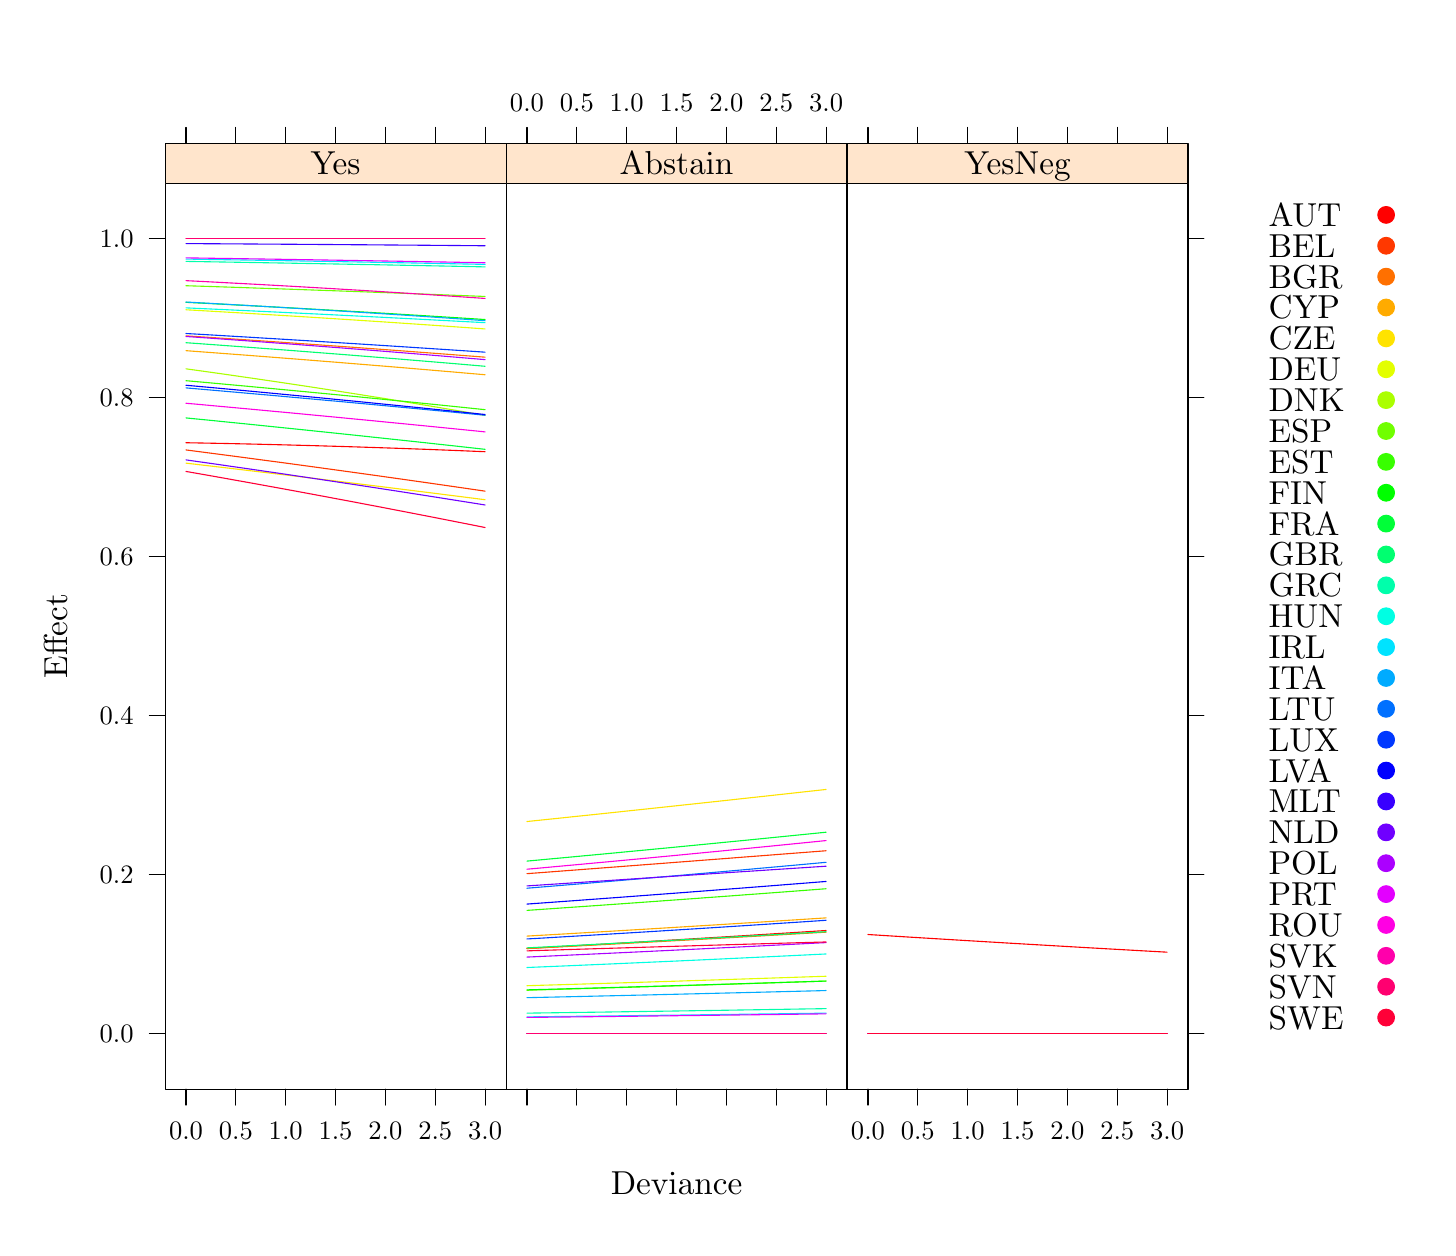
\begin{tikzpicture}[x=1pt,y=1pt]
\definecolor[named]{drawColor}{rgb}{0.00,0.00,0.00}
\definecolor[named]{fillColor}{rgb}{1.00,1.00,1.00}
\fill[color=fillColor,] (0,0) rectangle (505.89,433.62);
\begin{scope}
\path[clip] (  0.00,  0.00) rectangle (505.89,433.62);
\definecolor[named]{fillColor}{rgb}{0.00,0.00,0.00}
\end{scope}
\begin{scope}
\path[clip] (  0.00,  0.00) rectangle (505.89,433.62);
\definecolor[named]{fillColor}{rgb}{0.00,0.00,0.00}

\draw[fill opacity=0.00,draw opacity=0.00,] (  0.00,  0.00) rectangle (505.89,433.62);
\end{scope}
\begin{scope}
\path[clip] (  0.00,  0.00) rectangle (505.89,433.62);
\definecolor[named]{fillColor}{rgb}{0.00,0.00,0.00}
\end{scope}
\begin{scope}
\path[clip] (  0.00,  0.00) rectangle (505.89,433.62);
\definecolor[named]{fillColor}{rgb}{0.00,0.00,0.00}
\definecolor[named]{drawColor}{rgb}{0.00,0.00,0.00}

\node[color=drawColor,anchor=base,inner sep=0pt, outer sep=0pt, scale=  1.20] at (234.47, 12.04) {Deviance%
};
\end{scope}
\begin{scope}
\path[clip] (  0.00,  0.00) rectangle (505.89,433.62);
\definecolor[named]{fillColor}{rgb}{0.00,0.00,0.00}
\definecolor[named]{drawColor}{rgb}{0.00,0.00,0.00}

\node[rotate= 90.00,color=drawColor,anchor=base,inner sep=0pt, outer sep=0pt, scale=  1.20] at ( 14.29,213.72) {Effect%
};
\end{scope}
\begin{scope}
\path[clip] (  0.00,  0.00) rectangle (505.89,433.62);
\definecolor[named]{fillColor}{rgb}{0.00,0.00,0.00}
\end{scope}
\begin{scope}
\path[clip] (  0.00,  0.00) rectangle (505.89,433.62);
\definecolor[named]{fillColor}{rgb}{0.00,0.00,0.00}
\end{scope}
\begin{scope}
\path[clip] (  0.00,  0.00) rectangle (505.89,433.62);
\definecolor[named]{fillColor}{rgb}{0.00,0.00,0.00}
\end{scope}
\begin{scope}
\path[clip] ( 49.65, 50.02) rectangle (172.86,377.42);
\definecolor[named]{fillColor}{rgb}{0.00,0.00,0.00}
\end{scope}
\begin{scope}
\path[clip] (  0.00,  0.00) rectangle (505.89,433.62);
\definecolor[named]{fillColor}{rgb}{0.00,0.00,0.00}
\end{scope}
\begin{scope}
\path[clip] (  0.00,  0.00) rectangle (505.89,433.62);
\definecolor[named]{fillColor}{rgb}{0.00,0.00,0.00}
\definecolor[named]{drawColor}{rgb}{0.00,0.00,0.00}

\draw[color=drawColor,line cap=round,line join=round,fill opacity=0.00,] ( 57.21,391.87) -- ( 57.21,397.56);

\draw[color=drawColor,line cap=round,line join=round,fill opacity=0.00,] ( 75.22,391.87) -- ( 75.22,397.56);

\draw[color=drawColor,line cap=round,line join=round,fill opacity=0.00,] ( 93.24,391.87) -- ( 93.24,397.56);

\draw[color=drawColor,line cap=round,line join=round,fill opacity=0.00,] (111.25,391.87) -- (111.25,397.56);

\draw[color=drawColor,line cap=round,line join=round,fill opacity=0.00,] (129.27,391.87) -- (129.27,397.56);

\draw[color=drawColor,line cap=round,line join=round,fill opacity=0.00,] (147.28,391.87) -- (147.28,397.56);

\draw[color=drawColor,line cap=round,line join=round,fill opacity=0.00,] (165.29,391.87) -- (165.29,397.56);
\end{scope}
\begin{scope}
\path[clip] (  0.00,  0.00) rectangle (505.89,433.62);
\definecolor[named]{fillColor}{rgb}{0.00,0.00,0.00}
\end{scope}
\begin{scope}
\path[clip] (  0.00,  0.00) rectangle (505.89,433.62);
\definecolor[named]{fillColor}{rgb}{0.00,0.00,0.00}
\definecolor[named]{drawColor}{rgb}{0.00,0.00,0.00}

\draw[color=drawColor,line cap=round,line join=round,fill opacity=0.00,] ( 49.65, 70.12) -- ( 43.95, 70.12);

\draw[color=drawColor,line cap=round,line join=round,fill opacity=0.00,] ( 49.65,127.56) -- ( 43.95,127.56);

\draw[color=drawColor,line cap=round,line join=round,fill opacity=0.00,] ( 49.65,185.00) -- ( 43.95,185.00);

\draw[color=drawColor,line cap=round,line join=round,fill opacity=0.00,] ( 49.65,242.43) -- ( 43.95,242.43);

\draw[color=drawColor,line cap=round,line join=round,fill opacity=0.00,] ( 49.65,299.87) -- ( 43.95,299.87);

\draw[color=drawColor,line cap=round,line join=round,fill opacity=0.00,] ( 49.65,357.31) -- ( 43.95,357.31);

\node[color=drawColor,anchor=base east,inner sep=0pt, outer sep=0pt, scale=  0.96] at ( 38.26, 66.81) {0.0%
};

\node[color=drawColor,anchor=base east,inner sep=0pt, outer sep=0pt, scale=  0.96] at ( 38.26,124.25) {0.2%
};

\node[color=drawColor,anchor=base east,inner sep=0pt, outer sep=0pt, scale=  0.96] at ( 38.26,181.69) {0.4%
};

\node[color=drawColor,anchor=base east,inner sep=0pt, outer sep=0pt, scale=  0.96] at ( 38.26,239.13) {0.6%
};

\node[color=drawColor,anchor=base east,inner sep=0pt, outer sep=0pt, scale=  0.96] at ( 38.26,296.57) {0.8%
};

\node[color=drawColor,anchor=base east,inner sep=0pt, outer sep=0pt, scale=  0.96] at ( 38.26,354.01) {1.0%
};
\end{scope}
\begin{scope}
\path[clip] (  0.00,  0.00) rectangle (505.89,433.62);
\definecolor[named]{fillColor}{rgb}{0.00,0.00,0.00}
\end{scope}
\begin{scope}
\path[clip] (  0.00,  0.00) rectangle (505.89,433.62);
\definecolor[named]{fillColor}{rgb}{0.00,0.00,0.00}
\definecolor[named]{drawColor}{rgb}{0.00,0.00,0.00}

\draw[color=drawColor,line cap=round,line join=round,fill opacity=0.00,] ( 57.21, 50.02) -- ( 57.21, 44.32);

\draw[color=drawColor,line cap=round,line join=round,fill opacity=0.00,] ( 75.22, 50.02) -- ( 75.22, 44.32);

\draw[color=drawColor,line cap=round,line join=round,fill opacity=0.00,] ( 93.24, 50.02) -- ( 93.24, 44.32);

\draw[color=drawColor,line cap=round,line join=round,fill opacity=0.00,] (111.25, 50.02) -- (111.25, 44.32);

\draw[color=drawColor,line cap=round,line join=round,fill opacity=0.00,] (129.27, 50.02) -- (129.27, 44.32);

\draw[color=drawColor,line cap=round,line join=round,fill opacity=0.00,] (147.28, 50.02) -- (147.28, 44.32);

\draw[color=drawColor,line cap=round,line join=round,fill opacity=0.00,] (165.29, 50.02) -- (165.29, 44.32);

\node[color=drawColor,anchor=base,inner sep=0pt, outer sep=0pt, scale=  0.96] at ( 57.21, 32.02) {0.0%
};

\node[color=drawColor,anchor=base,inner sep=0pt, outer sep=0pt, scale=  0.96] at ( 75.22, 32.02) {0.5%
};

\node[color=drawColor,anchor=base,inner sep=0pt, outer sep=0pt, scale=  0.96] at ( 93.24, 32.02) {1.0%
};

\node[color=drawColor,anchor=base,inner sep=0pt, outer sep=0pt, scale=  0.96] at (111.25, 32.02) {1.5%
};

\node[color=drawColor,anchor=base,inner sep=0pt, outer sep=0pt, scale=  0.96] at (129.27, 32.02) {2.0%
};

\node[color=drawColor,anchor=base,inner sep=0pt, outer sep=0pt, scale=  0.96] at (147.28, 32.02) {2.5%
};

\node[color=drawColor,anchor=base,inner sep=0pt, outer sep=0pt, scale=  0.96] at (165.29, 32.02) {3.0%
};
\end{scope}
\begin{scope}
\path[clip] (  0.00,  0.00) rectangle (505.89,433.62);
\definecolor[named]{fillColor}{rgb}{0.00,0.00,0.00}
\end{scope}
\begin{scope}
\path[clip] ( 49.65, 50.02) rectangle (172.86,377.42);
\definecolor[named]{fillColor}{rgb}{0.00,0.00,0.00}
\definecolor[named]{drawColor}{rgb}{1.00,0.00,0.00}

\draw[color=drawColor,line cap=round,line join=round,fill opacity=0.00,] ( 57.21,283.63) --
	( 60.81,283.57) --
	( 64.42,283.50) --
	( 68.02,283.43) --
	( 71.62,283.36) --
	( 75.22,283.28) --
	( 78.83,283.20) --
	( 82.43,283.12) --
	( 86.03,283.03) --
	( 89.64,282.94) --
	( 93.24,282.85) --
	( 96.84,282.75) --
	(100.44,282.66) --
	(104.05,282.56) --
	(107.65,282.45) --
	(111.25,282.35) --
	(114.85,282.24) --
	(118.46,282.13) --
	(122.06,282.01) --
	(125.66,281.89) --
	(129.27,281.77) --
	(132.87,281.65) --
	(136.47,281.52) --
	(140.07,281.39) --
	(143.68,281.26) --
	(147.28,281.12) --
	(150.88,280.98) --
	(154.49,280.84) --
	(158.09,280.69) --
	(161.69,280.54) --
	(165.29,280.39);
\definecolor[named]{drawColor}{rgb}{1.00,0.22,0.00}

\draw[color=drawColor,line cap=round,line join=round,fill opacity=0.00,] ( 57.21,281.03) --
	( 60.81,280.56) --
	( 64.42,280.09) --
	( 68.02,279.62) --
	( 71.62,279.15) --
	( 75.22,278.68) --
	( 78.83,278.20) --
	( 82.43,277.72) --
	( 86.03,277.24) --
	( 89.64,276.76) --
	( 93.24,276.28) --
	( 96.84,275.79) --
	(100.44,275.30) --
	(104.05,274.81) --
	(107.65,274.31) --
	(111.25,273.82) --
	(114.85,273.32) --
	(118.46,272.82) --
	(122.06,272.32) --
	(125.66,271.82) --
	(129.27,271.31) --
	(132.87,270.80) --
	(136.47,270.29) --
	(140.07,269.78) --
	(143.68,269.27) --
	(147.28,268.75) --
	(150.88,268.23) --
	(154.49,267.71) --
	(158.09,267.19) --
	(161.69,266.66) --
	(165.29,266.14);
\definecolor[named]{drawColor}{rgb}{1.00,0.44,0.00}

\draw[color=drawColor,line cap=round,line join=round,fill opacity=0.00,] ( 57.21,322.26) --
	( 60.81,322.02) --
	( 64.42,321.79) --
	( 68.02,321.55) --
	( 71.62,321.31) --
	( 75.22,321.07) --
	( 78.83,320.83) --
	( 82.43,320.58) --
	( 86.03,320.34) --
	( 89.64,320.09) --
	( 93.24,319.84) --
	( 96.84,319.59) --
	(100.44,319.34) --
	(104.05,319.09) --
	(107.65,318.83) --
	(111.25,318.58) --
	(114.85,318.32) --
	(118.46,318.06) --
	(122.06,317.80) --
	(125.66,317.54) --
	(129.27,317.27) --
	(132.87,317.01) --
	(136.47,316.74) --
	(140.07,316.47) --
	(143.68,316.20) --
	(147.28,315.93) --
	(150.88,315.66) --
	(154.49,315.38) --
	(158.09,315.10) --
	(161.69,314.83) --
	(165.29,314.55);
\definecolor[named]{drawColor}{rgb}{1.00,0.67,0.00}

\draw[color=drawColor,line cap=round,line join=round,fill opacity=0.00,] ( 57.21,316.90) --
	( 60.81,316.63) --
	( 64.42,316.36) --
	( 68.02,316.09) --
	( 71.62,315.82) --
	( 75.22,315.55) --
	( 78.83,315.28) --
	( 82.43,315.00) --
	( 86.03,314.72) --
	( 89.64,314.44) --
	( 93.24,314.16) --
	( 96.84,313.88) --
	(100.44,313.60) --
	(104.05,313.31) --
	(107.65,313.02) --
	(111.25,312.74) --
	(114.85,312.44) --
	(118.46,312.15) --
	(122.06,311.86) --
	(125.66,311.56) --
	(129.27,311.27) --
	(132.87,310.97) --
	(136.47,310.67) --
	(140.07,310.36) --
	(143.68,310.06) --
	(147.28,309.75) --
	(150.88,309.44) --
	(154.49,309.14) --
	(158.09,308.82) --
	(161.69,308.51) --
	(165.29,308.20);
\definecolor[named]{drawColor}{rgb}{1.00,0.89,0.00}

\draw[color=drawColor,line cap=round,line join=round,fill opacity=0.00,] ( 57.21,276.26) --
	( 60.81,275.84) --
	( 64.42,275.41) --
	( 68.02,274.99) --
	( 71.62,274.57) --
	( 75.22,274.14) --
	( 78.83,273.71) --
	( 82.43,273.28) --
	( 86.03,272.85) --
	( 89.64,272.42) --
	( 93.24,271.99) --
	( 96.84,271.55) --
	(100.44,271.12) --
	(104.05,270.68) --
	(107.65,270.24) --
	(111.25,269.80) --
	(114.85,269.36) --
	(118.46,268.92) --
	(122.06,268.47) --
	(125.66,268.03) --
	(129.27,267.58) --
	(132.87,267.13) --
	(136.47,266.68) --
	(140.07,266.23) --
	(143.68,265.78) --
	(147.28,265.33) --
	(150.88,264.87) --
	(154.49,264.42) --
	(158.09,263.96) --
	(161.69,263.50) --
	(165.29,263.04);
\definecolor[named]{drawColor}{rgb}{0.89,1.00,0.00}

\draw[color=drawColor,line cap=round,line join=round,fill opacity=0.00,] ( 57.21,331.68) --
	( 60.81,331.48) --
	( 64.42,331.27) --
	( 68.02,331.06) --
	( 71.62,330.85) --
	( 75.22,330.64) --
	( 78.83,330.43) --
	( 82.43,330.21) --
	( 86.03,329.99) --
	( 89.64,329.77) --
	( 93.24,329.55) --
	( 96.84,329.33) --
	(100.44,329.11) --
	(104.05,328.88) --
	(107.65,328.65) --
	(111.25,328.42) --
	(114.85,328.19) --
	(118.46,327.96) --
	(122.06,327.72) --
	(125.66,327.49) --
	(129.27,327.25) --
	(132.87,327.01) --
	(136.47,326.76) --
	(140.07,326.52) --
	(143.68,326.27) --
	(147.28,326.03) --
	(150.88,325.78) --
	(154.49,325.52) --
	(158.09,325.27) --
	(161.69,325.01) --
	(165.29,324.75);
\definecolor[named]{drawColor}{rgb}{0.67,1.00,0.00}

\draw[color=drawColor,line cap=round,line join=round,fill opacity=0.00,] ( 57.21,310.34) --
	( 60.81,309.84) --
	( 64.42,309.34) --
	( 68.02,308.83) --
	( 71.62,308.32) --
	( 75.22,307.80) --
	( 78.83,307.28) --
	( 82.43,306.76) --
	( 86.03,306.23) --
	( 89.64,305.70) --
	( 93.24,305.16) --
	( 96.84,304.62) --
	(100.44,304.08) --
	(104.05,303.53) --
	(107.65,302.97) --
	(111.25,302.41) --
	(114.85,301.85) --
	(118.46,301.28) --
	(122.06,300.71) --
	(125.66,300.14) --
	(129.27,299.56) --
	(132.87,298.97) --
	(136.47,298.38) --
	(140.07,297.79) --
	(143.68,297.19) --
	(147.28,296.59) --
	(150.88,295.98) --
	(154.49,295.37) --
	(158.09,294.75) --
	(161.69,294.13) --
	(165.29,293.51);
\definecolor[named]{drawColor}{rgb}{0.44,1.00,0.00}

\draw[color=drawColor,line cap=round,line join=round,fill opacity=0.00,] ( 57.21,340.37) --
	( 60.81,340.25) --
	( 64.42,340.14) --
	( 68.02,340.02) --
	( 71.62,339.90) --
	( 75.22,339.78) --
	( 78.83,339.66) --
	( 82.43,339.53) --
	( 86.03,339.41) --
	( 89.64,339.29) --
	( 93.24,339.16) --
	( 96.84,339.04) --
	(100.44,338.91) --
	(104.05,338.78) --
	(107.65,338.66) --
	(111.25,338.53) --
	(114.85,338.40) --
	(118.46,338.27) --
	(122.06,338.14) --
	(125.66,338.00) --
	(129.27,337.87) --
	(132.87,337.74) --
	(136.47,337.60) --
	(140.07,337.46) --
	(143.68,337.33) --
	(147.28,337.19) --
	(150.88,337.05) --
	(154.49,336.91) --
	(158.09,336.77) --
	(161.69,336.63) --
	(165.29,336.49);
\definecolor[named]{drawColor}{rgb}{0.22,1.00,0.00}

\draw[color=drawColor,line cap=round,line join=round,fill opacity=0.00,] ( 57.21,306.05) --
	( 60.81,305.73) --
	( 64.42,305.41) --
	( 68.02,305.08) --
	( 71.62,304.75) --
	( 75.22,304.42) --
	( 78.83,304.09) --
	( 82.43,303.75) --
	( 86.03,303.42) --
	( 89.64,303.08) --
	( 93.24,302.74) --
	( 96.84,302.40) --
	(100.44,302.06) --
	(104.05,301.71) --
	(107.65,301.37) --
	(111.25,301.02) --
	(114.85,300.67) --
	(118.46,300.32) --
	(122.06,299.96) --
	(125.66,299.61) --
	(129.27,299.25) --
	(132.87,298.89) --
	(136.47,298.53) --
	(140.07,298.17) --
	(143.68,297.80) --
	(147.28,297.44) --
	(150.88,297.07) --
	(154.49,296.70) --
	(158.09,296.33) --
	(161.69,295.95) --
	(165.29,295.58);
\definecolor[named]{drawColor}{rgb}{0.00,1.00,0.00}

\draw[color=drawColor,line cap=round,line join=round,fill opacity=0.00,] ( 57.21,334.37) --
	( 60.81,334.18) --
	( 64.42,334.00) --
	( 68.02,333.81) --
	( 71.62,333.62) --
	( 75.22,333.43) --
	( 78.83,333.24) --
	( 82.43,333.05) --
	( 86.03,332.85) --
	( 89.64,332.66) --
	( 93.24,332.46) --
	( 96.84,332.26) --
	(100.44,332.06) --
	(104.05,331.85) --
	(107.65,331.65) --
	(111.25,331.44) --
	(114.85,331.24) --
	(118.46,331.03) --
	(122.06,330.82) --
	(125.66,330.60) --
	(129.27,330.39) --
	(132.87,330.17) --
	(136.47,329.95) --
	(140.07,329.73) --
	(143.68,329.51) --
	(147.28,329.29) --
	(150.88,329.06) --
	(154.49,328.84) --
	(158.09,328.61) --
	(161.69,328.38) --
	(165.29,328.15);
\definecolor[named]{drawColor}{rgb}{0.00,1.00,0.22}

\draw[color=drawColor,line cap=round,line join=round,fill opacity=0.00,] ( 57.21,292.60) --
	( 60.81,292.24) --
	( 64.42,291.89) --
	( 68.02,291.53) --
	( 71.62,291.16) --
	( 75.22,290.80) --
	( 78.83,290.44) --
	( 82.43,290.07) --
	( 86.03,289.70) --
	( 89.64,289.33) --
	( 93.24,288.96) --
	( 96.84,288.59) --
	(100.44,288.22) --
	(104.05,287.84) --
	(107.65,287.47) --
	(111.25,287.09) --
	(114.85,286.71) --
	(118.46,286.33) --
	(122.06,285.95) --
	(125.66,285.56) --
	(129.27,285.18) --
	(132.87,284.79) --
	(136.47,284.41) --
	(140.07,284.02) --
	(143.68,283.63) --
	(147.28,283.23) --
	(150.88,282.84) --
	(154.49,282.45) --
	(158.09,282.05) --
	(161.69,281.65) --
	(165.29,281.25);
\definecolor[named]{drawColor}{rgb}{0.00,1.00,0.44}

\draw[color=drawColor,line cap=round,line join=round,fill opacity=0.00,] ( 57.21,319.78) --
	( 60.81,319.52) --
	( 64.42,319.26) --
	( 68.02,319.00) --
	( 71.62,318.73) --
	( 75.22,318.47) --
	( 78.83,318.20) --
	( 82.43,317.93) --
	( 86.03,317.66) --
	( 89.64,317.39) --
	( 93.24,317.12) --
	( 96.84,316.84) --
	(100.44,316.56) --
	(104.05,316.28) --
	(107.65,316.00) --
	(111.25,315.72) --
	(114.85,315.44) --
	(118.46,315.15) --
	(122.06,314.86) --
	(125.66,314.57) --
	(129.27,314.28) --
	(132.87,313.99) --
	(136.47,313.69) --
	(140.07,313.39) --
	(143.68,313.09) --
	(147.28,312.79) --
	(150.88,312.49) --
	(154.49,312.19) --
	(158.09,311.88) --
	(161.69,311.57) --
	(165.29,311.26);
\definecolor[named]{drawColor}{rgb}{0.00,1.00,0.67}

\draw[color=drawColor,line cap=round,line join=round,fill opacity=0.00,] ( 57.21,349.16) --
	( 60.81,349.10) --
	( 64.42,349.04) --
	( 68.02,348.98) --
	( 71.62,348.92) --
	( 75.22,348.86) --
	( 78.83,348.80) --
	( 82.43,348.74) --
	( 86.03,348.67) --
	( 89.64,348.61) --
	( 93.24,348.55) --
	( 96.84,348.48) --
	(100.44,348.42) --
	(104.05,348.36) --
	(107.65,348.29) --
	(111.25,348.22) --
	(114.85,348.16) --
	(118.46,348.09) --
	(122.06,348.02) --
	(125.66,347.96) --
	(129.27,347.89) --
	(132.87,347.82) --
	(136.47,347.75) --
	(140.07,347.68) --
	(143.68,347.61) --
	(147.28,347.54) --
	(150.88,347.47) --
	(154.49,347.40) --
	(158.09,347.33) --
	(161.69,347.25) --
	(165.29,347.18);
\definecolor[named]{drawColor}{rgb}{0.00,1.00,0.89}

\draw[color=drawColor,line cap=round,line join=round,fill opacity=0.00,] ( 57.21,332.37) --
	( 60.81,332.20) --
	( 64.42,332.04) --
	( 68.02,331.87) --
	( 71.62,331.71) --
	( 75.22,331.54) --
	( 78.83,331.37) --
	( 82.43,331.20) --
	( 86.03,331.03) --
	( 89.64,330.86) --
	( 93.24,330.69) --
	( 96.84,330.52) --
	(100.44,330.34) --
	(104.05,330.17) --
	(107.65,329.99) --
	(111.25,329.81) --
	(114.85,329.63) --
	(118.46,329.45) --
	(122.06,329.27) --
	(125.66,329.09) --
	(129.27,328.91) --
	(132.87,328.72) --
	(136.47,328.54) --
	(140.07,328.35) --
	(143.68,328.16) --
	(147.28,327.97) --
	(150.88,327.78) --
	(154.49,327.59) --
	(158.09,327.40) --
	(161.69,327.21) --
	(165.29,327.01);
\definecolor[named]{drawColor}{rgb}{0.00,0.89,1.00}

\draw[color=drawColor,line cap=round,line join=round,fill opacity=0.00,] ( 57.21,349.99) --
	( 60.81,349.94) --
	( 64.42,349.88) --
	( 68.02,349.82) --
	( 71.62,349.76) --
	( 75.22,349.71) --
	( 78.83,349.65) --
	( 82.43,349.59) --
	( 86.03,349.53) --
	( 89.64,349.47) --
	( 93.24,349.41) --
	( 96.84,349.35) --
	(100.44,349.28) --
	(104.05,349.22) --
	(107.65,349.16) --
	(111.25,349.10) --
	(114.85,349.03) --
	(118.46,348.97) --
	(122.06,348.90) --
	(125.66,348.84) --
	(129.27,348.77) --
	(132.87,348.70) --
	(136.47,348.64) --
	(140.07,348.57) --
	(143.68,348.50) --
	(147.28,348.43) --
	(150.88,348.36) --
	(154.49,348.29) --
	(158.09,348.22) --
	(161.69,348.15) --
	(165.29,348.08);
\definecolor[named]{drawColor}{rgb}{0.00,0.67,1.00}

\draw[color=drawColor,line cap=round,line join=round,fill opacity=0.00,] ( 57.21,334.48) --
	( 60.81,334.28) --
	( 64.42,334.08) --
	( 68.02,333.88) --
	( 71.62,333.68) --
	( 75.22,333.47) --
	( 78.83,333.27) --
	( 82.43,333.06) --
	( 86.03,332.85) --
	( 89.64,332.64) --
	( 93.24,332.42) --
	( 96.84,332.21) --
	(100.44,331.99) --
	(104.05,331.77) --
	(107.65,331.55) --
	(111.25,331.33) --
	(114.85,331.10) --
	(118.46,330.87) --
	(122.06,330.64) --
	(125.66,330.41) --
	(129.27,330.18) --
	(132.87,329.94) --
	(136.47,329.71) --
	(140.07,329.47) --
	(143.68,329.23) --
	(147.28,328.98) --
	(150.88,328.74) --
	(154.49,328.49) --
	(158.09,328.24) --
	(161.69,327.99) --
	(165.29,327.73);
\definecolor[named]{drawColor}{rgb}{0.00,0.44,1.00}

\draw[color=drawColor,line cap=round,line join=round,fill opacity=0.00,] ( 57.21,303.45) --
	( 60.81,303.14) --
	( 64.42,302.83) --
	( 68.02,302.52) --
	( 71.62,302.20) --
	( 75.22,301.89) --
	( 78.83,301.57) --
	( 82.43,301.25) --
	( 86.03,300.94) --
	( 89.64,300.62) --
	( 93.24,300.29) --
	( 96.84,299.97) --
	(100.44,299.65) --
	(104.05,299.32) --
	(107.65,298.99) --
	(111.25,298.67) --
	(114.85,298.34) --
	(118.46,298.00) --
	(122.06,297.67) --
	(125.66,297.34) --
	(129.27,297.00) --
	(132.87,296.66) --
	(136.47,296.32) --
	(140.07,295.99) --
	(143.68,295.64) --
	(147.28,295.30) --
	(150.88,294.96) --
	(154.49,294.61) --
	(158.09,294.26) --
	(161.69,293.92) --
	(165.29,293.57);
\definecolor[named]{drawColor}{rgb}{0.00,0.22,1.00}

\draw[color=drawColor,line cap=round,line join=round,fill opacity=0.00,] ( 57.21,323.10) --
	( 60.81,322.90) --
	( 64.42,322.69) --
	( 68.02,322.48) --
	( 71.62,322.26) --
	( 75.22,322.05) --
	( 78.83,321.84) --
	( 82.43,321.62) --
	( 86.03,321.40) --
	( 89.64,321.19) --
	( 93.24,320.97) --
	( 96.84,320.75) --
	(100.44,320.53) --
	(104.05,320.31) --
	(107.65,320.08) --
	(111.25,319.86) --
	(114.85,319.63) --
	(118.46,319.41) --
	(122.06,319.18) --
	(125.66,318.95) --
	(129.27,318.72) --
	(132.87,318.49) --
	(136.47,318.26) --
	(140.07,318.02) --
	(143.68,317.79) --
	(147.28,317.55) --
	(150.88,317.32) --
	(154.49,317.08) --
	(158.09,316.84) --
	(161.69,316.60) --
	(165.29,316.35);
\definecolor[named]{drawColor}{rgb}{0.00,0.00,1.00}

\draw[color=drawColor,line cap=round,line join=round,fill opacity=0.00,] ( 57.21,304.40) --
	( 60.81,304.08) --
	( 64.42,303.75) --
	( 68.02,303.42) --
	( 71.62,303.09) --
	( 75.22,302.75) --
	( 78.83,302.42) --
	( 82.43,302.08) --
	( 86.03,301.74) --
	( 89.64,301.40) --
	( 93.24,301.05) --
	( 96.84,300.71) --
	(100.44,300.36) --
	(104.05,300.02) --
	(107.65,299.67) --
	(111.25,299.31) --
	(114.85,298.96) --
	(118.46,298.61) --
	(122.06,298.25) --
	(125.66,297.89) --
	(129.27,297.53) --
	(132.87,297.17) --
	(136.47,296.80) --
	(140.07,296.44) --
	(143.68,296.07) --
	(147.28,295.70) --
	(150.88,295.33) --
	(154.49,294.96) --
	(158.09,294.58) --
	(161.69,294.21) --
	(165.29,293.83);
\definecolor[named]{drawColor}{rgb}{0.22,0.00,1.00}

\draw[color=drawColor,line cap=round,line join=round,fill opacity=0.00,] ( 57.21,355.59) --
	( 60.81,355.57) --
	( 64.42,355.55) --
	( 68.02,355.53) --
	( 71.62,355.50) --
	( 75.22,355.48) --
	( 78.83,355.46) --
	( 82.43,355.43) --
	( 86.03,355.41) --
	( 89.64,355.39) --
	( 93.24,355.36) --
	( 96.84,355.34) --
	(100.44,355.31) --
	(104.05,355.29) --
	(107.65,355.26) --
	(111.25,355.24) --
	(114.85,355.21) --
	(118.46,355.18) --
	(122.06,355.16) --
	(125.66,355.13) --
	(129.27,355.10) --
	(132.87,355.07) --
	(136.47,355.05) --
	(140.07,355.02) --
	(143.68,354.99) --
	(147.28,354.96) --
	(150.88,354.93) --
	(154.49,354.90) --
	(158.09,354.87) --
	(161.69,354.84) --
	(165.29,354.81);
\definecolor[named]{drawColor}{rgb}{0.44,0.00,1.00}

\draw[color=drawColor,line cap=round,line join=round,fill opacity=0.00,] ( 57.21,277.43) --
	( 60.81,276.92) --
	( 64.42,276.41) --
	( 68.02,275.90) --
	( 71.62,275.38) --
	( 75.22,274.86) --
	( 78.83,274.34) --
	( 82.43,273.82) --
	( 86.03,273.29) --
	( 89.64,272.77) --
	( 93.24,272.24) --
	( 96.84,271.70) --
	(100.44,271.17) --
	(104.05,270.63) --
	(107.65,270.09) --
	(111.25,269.55) --
	(114.85,269.00) --
	(118.46,268.46) --
	(122.06,267.91) --
	(125.66,267.36) --
	(129.27,266.80) --
	(132.87,266.25) --
	(136.47,265.69) --
	(140.07,265.13) --
	(143.68,264.57) --
	(147.28,264.00) --
	(150.88,263.43) --
	(154.49,262.86) --
	(158.09,262.29) --
	(161.69,261.72) --
	(165.29,261.14);
\definecolor[named]{drawColor}{rgb}{0.67,0.00,1.00}

\draw[color=drawColor,line cap=round,line join=round,fill opacity=0.00,] ( 57.21,322.03) --
	( 60.81,321.78) --
	( 64.42,321.53) --
	( 68.02,321.27) --
	( 71.62,321.01) --
	( 75.22,320.75) --
	( 78.83,320.49) --
	( 82.43,320.23) --
	( 86.03,319.96) --
	( 89.64,319.69) --
	( 93.24,319.43) --
	( 96.84,319.16) --
	(100.44,318.88) --
	(104.05,318.61) --
	(107.65,318.33) --
	(111.25,318.06) --
	(114.85,317.78) --
	(118.46,317.49) --
	(122.06,317.21) --
	(125.66,316.93) --
	(129.27,316.64) --
	(132.87,316.35) --
	(136.47,316.06) --
	(140.07,315.77) --
	(143.68,315.47) --
	(147.28,315.17) --
	(150.88,314.87) --
	(154.49,314.57) --
	(158.09,314.27) --
	(161.69,313.97) --
	(165.29,313.66);
\definecolor[named]{drawColor}{rgb}{0.89,0.00,1.00}

\draw[color=drawColor,line cap=round,line join=round,fill opacity=0.00,] ( 57.21,350.43) --
	( 60.81,350.38) --
	( 64.42,350.33) --
	( 68.02,350.27) --
	( 71.62,350.22) --
	( 75.22,350.17) --
	( 78.83,350.11) --
	( 82.43,350.06) --
	( 86.03,350.00) --
	( 89.64,349.95) --
	( 93.24,349.89) --
	( 96.84,349.83) --
	(100.44,349.78) --
	(104.05,349.72) --
	(107.65,349.66) --
	(111.25,349.60) --
	(114.85,349.54) --
	(118.46,349.48) --
	(122.06,349.42) --
	(125.66,349.36) --
	(129.27,349.30) --
	(132.87,349.24) --
	(136.47,349.18) --
	(140.07,349.12) --
	(143.68,349.05) --
	(147.28,348.99) --
	(150.88,348.93) --
	(154.49,348.86) --
	(158.09,348.80) --
	(161.69,348.73) --
	(165.29,348.67);
\definecolor[named]{drawColor}{rgb}{1.00,0.00,0.89}

\draw[color=drawColor,line cap=round,line join=round,fill opacity=0.00,] ( 57.21,297.90) --
	( 60.81,297.58) --
	( 64.42,297.25) --
	( 68.02,296.92) --
	( 71.62,296.59) --
	( 75.22,296.26) --
	( 78.83,295.93) --
	( 82.43,295.59) --
	( 86.03,295.26) --
	( 89.64,294.92) --
	( 93.24,294.59) --
	( 96.84,294.25) --
	(100.44,293.91) --
	(104.05,293.56) --
	(107.65,293.22) --
	(111.25,292.88) --
	(114.85,292.53) --
	(118.46,292.18) --
	(122.06,291.84) --
	(125.66,291.49) --
	(129.27,291.13) --
	(132.87,290.78) --
	(136.47,290.43) --
	(140.07,290.07) --
	(143.68,289.72) --
	(147.28,289.36) --
	(150.88,289.00) --
	(154.49,288.64) --
	(158.09,288.28) --
	(161.69,287.92) --
	(165.29,287.55);
\definecolor[named]{drawColor}{rgb}{1.00,0.00,0.67}

\draw[color=drawColor,line cap=round,line join=round,fill opacity=0.00,] ( 57.21,342.20) --
	( 60.81,342.02) --
	( 64.42,341.84) --
	( 68.02,341.65) --
	( 71.62,341.46) --
	( 75.22,341.27) --
	( 78.83,341.08) --
	( 82.43,340.89) --
	( 86.03,340.69) --
	( 89.64,340.49) --
	( 93.24,340.29) --
	( 96.84,340.09) --
	(100.44,339.88) --
	(104.05,339.67) --
	(107.65,339.46) --
	(111.25,339.25) --
	(114.85,339.03) --
	(118.46,338.82) --
	(122.06,338.60) --
	(125.66,338.38) --
	(129.27,338.15) --
	(132.87,337.92) --
	(136.47,337.69) --
	(140.07,337.46) --
	(143.68,337.23) --
	(147.28,336.99) --
	(150.88,336.75) --
	(154.49,336.51) --
	(158.09,336.26) --
	(161.69,336.02) --
	(165.29,335.77);
\definecolor[named]{drawColor}{rgb}{1.00,0.00,0.44}

\draw[color=drawColor,line cap=round,line join=round,fill opacity=0.00,] ( 57.21,357.31) --
	( 60.81,357.31) --
	( 64.42,357.31) --
	( 68.02,357.31) --
	( 71.62,357.31) --
	( 75.22,357.31) --
	( 78.83,357.31) --
	( 82.43,357.31) --
	( 86.03,357.31) --
	( 89.64,357.31) --
	( 93.24,357.31) --
	( 96.84,357.31) --
	(100.44,357.31) --
	(104.05,357.31) --
	(107.65,357.31) --
	(111.25,357.31) --
	(114.85,357.31) --
	(118.46,357.31) --
	(122.06,357.31) --
	(125.66,357.31) --
	(129.27,357.31) --
	(132.87,357.31) --
	(136.47,357.31) --
	(140.07,357.31) --
	(143.68,357.31) --
	(147.28,357.31) --
	(150.88,357.31) --
	(154.49,357.31) --
	(158.09,357.31) --
	(161.69,357.31) --
	(165.29,357.31);
\definecolor[named]{drawColor}{rgb}{1.00,0.00,0.22}

\draw[color=drawColor,line cap=round,line join=round,fill opacity=0.00,] ( 57.21,273.26) --
	( 60.81,272.63) --
	( 64.42,272.00) --
	( 68.02,271.36) --
	( 71.62,270.72) --
	( 75.22,270.07) --
	( 78.83,269.43) --
	( 82.43,268.78) --
	( 86.03,268.12) --
	( 89.64,267.47) --
	( 93.24,266.81) --
	( 96.84,266.15) --
	(100.44,265.48) --
	(104.05,264.81) --
	(107.65,264.14) --
	(111.25,263.46) --
	(114.85,262.79) --
	(118.46,262.11) --
	(122.06,261.42) --
	(125.66,260.74) --
	(129.27,260.05) --
	(132.87,259.35) --
	(136.47,258.66) --
	(140.07,257.96) --
	(143.68,257.26) --
	(147.28,256.56) --
	(150.88,255.85) --
	(154.49,255.14) --
	(158.09,254.43) --
	(161.69,253.72) --
	(165.29,253.00);
\end{scope}
\begin{scope}
\path[clip] (  0.00,  0.00) rectangle (505.89,433.62);
\definecolor[named]{fillColor}{rgb}{0.00,0.00,0.00}
\end{scope}
\begin{scope}
\path[clip] (  0.00,  0.00) rectangle (505.89,433.62);
\definecolor[named]{fillColor}{rgb}{0.00,0.00,0.00}
\definecolor[named]{drawColor}{rgb}{0.00,0.00,0.00}

\draw[color=drawColor,line cap=round,line join=round,fill opacity=0.00,] ( 49.65, 50.02) rectangle (172.86,377.42);
\end{scope}
\begin{scope}
\path[clip] (  0.00,  0.00) rectangle (505.89,433.62);
\definecolor[named]{fillColor}{rgb}{0.00,0.00,0.00}
\end{scope}
\begin{scope}
\path[clip] (  0.00,  0.00) rectangle (505.89,433.62);
\definecolor[named]{fillColor}{rgb}{0.00,0.00,0.00}
\end{scope}
\begin{scope}
\path[clip] ( 49.65,377.42) rectangle (172.86,391.87);
\definecolor[named]{fillColor}{rgb}{0.00,0.00,0.00}
\definecolor[named]{drawColor}{rgb}{1.00,0.90,0.80}
\definecolor[named]{fillColor}{rgb}{1.00,0.90,0.80}

\draw[color=drawColor,line cap=round,line join=round,fill=fillColor,] ( 49.65,377.42) rectangle (172.86,391.87);
\definecolor[named]{drawColor}{rgb}{0.00,0.00,0.00}

\node[color=drawColor,anchor=base west,inner sep=0pt, outer sep=0pt, scale=  1.20] at (102.22,380.51) {Yes%
};
\end{scope}
\begin{scope}
\path[clip] (  0.00,  0.00) rectangle (505.89,433.62);
\definecolor[named]{fillColor}{rgb}{0.00,0.00,0.00}
\end{scope}
\begin{scope}
\path[clip] (  0.00,  0.00) rectangle (505.89,433.62);
\definecolor[named]{fillColor}{rgb}{0.00,0.00,0.00}
\definecolor[named]{drawColor}{rgb}{0.00,0.00,0.00}

\draw[color=drawColor,line cap=round,line join=round,fill opacity=0.00,] ( 49.65,377.42) rectangle (172.86,391.87);
\end{scope}
\begin{scope}
\path[clip] (  0.00,  0.00) rectangle (505.89,433.62);
\definecolor[named]{fillColor}{rgb}{0.00,0.00,0.00}
\end{scope}
\begin{scope}
\path[clip] (  0.00,  0.00) rectangle (505.89,433.62);
\definecolor[named]{fillColor}{rgb}{0.00,0.00,0.00}
\end{scope}
\begin{scope}
\path[clip] (172.86, 50.02) rectangle (296.07,377.42);
\definecolor[named]{fillColor}{rgb}{0.00,0.00,0.00}
\end{scope}
\begin{scope}
\path[clip] (  0.00,  0.00) rectangle (505.89,433.62);
\definecolor[named]{fillColor}{rgb}{0.00,0.00,0.00}
\end{scope}
\begin{scope}
\path[clip] (  0.00,  0.00) rectangle (505.89,433.62);
\definecolor[named]{fillColor}{rgb}{0.00,0.00,0.00}
\definecolor[named]{drawColor}{rgb}{0.00,0.00,0.00}

\draw[color=drawColor,line cap=round,line join=round,fill opacity=0.00,] (180.42,391.87) -- (180.42,397.56);

\draw[color=drawColor,line cap=round,line join=round,fill opacity=0.00,] (198.44,391.87) -- (198.44,397.56);

\draw[color=drawColor,line cap=round,line join=round,fill opacity=0.00,] (216.45,391.87) -- (216.45,397.56);

\draw[color=drawColor,line cap=round,line join=round,fill opacity=0.00,] (234.47,391.87) -- (234.47,397.56);

\draw[color=drawColor,line cap=round,line join=round,fill opacity=0.00,] (252.48,391.87) -- (252.48,397.56);

\draw[color=drawColor,line cap=round,line join=round,fill opacity=0.00,] (270.49,391.87) -- (270.49,397.56);

\draw[color=drawColor,line cap=round,line join=round,fill opacity=0.00,] (288.51,391.87) -- (288.51,397.56);

\node[color=drawColor,anchor=base,inner sep=0pt, outer sep=0pt, scale=  0.96] at (180.42,403.25) {0.0%
};

\node[color=drawColor,anchor=base,inner sep=0pt, outer sep=0pt, scale=  0.96] at (198.44,403.25) {0.5%
};

\node[color=drawColor,anchor=base,inner sep=0pt, outer sep=0pt, scale=  0.96] at (216.45,403.25) {1.0%
};

\node[color=drawColor,anchor=base,inner sep=0pt, outer sep=0pt, scale=  0.96] at (234.47,403.25) {1.5%
};

\node[color=drawColor,anchor=base,inner sep=0pt, outer sep=0pt, scale=  0.96] at (252.48,403.25) {2.0%
};

\node[color=drawColor,anchor=base,inner sep=0pt, outer sep=0pt, scale=  0.96] at (270.49,403.25) {2.5%
};

\node[color=drawColor,anchor=base,inner sep=0pt, outer sep=0pt, scale=  0.96] at (288.51,403.25) {3.0%
};
\end{scope}
\begin{scope}
\path[clip] (  0.00,  0.00) rectangle (505.89,433.62);
\definecolor[named]{fillColor}{rgb}{0.00,0.00,0.00}
\end{scope}
\begin{scope}
\path[clip] (  0.00,  0.00) rectangle (505.89,433.62);
\definecolor[named]{fillColor}{rgb}{0.00,0.00,0.00}
\end{scope}
\begin{scope}
\path[clip] (  0.00,  0.00) rectangle (505.89,433.62);
\definecolor[named]{fillColor}{rgb}{0.00,0.00,0.00}
\end{scope}
\begin{scope}
\path[clip] (  0.00,  0.00) rectangle (505.89,433.62);
\definecolor[named]{fillColor}{rgb}{0.00,0.00,0.00}
\definecolor[named]{drawColor}{rgb}{0.00,0.00,0.00}

\draw[color=drawColor,line cap=round,line join=round,fill opacity=0.00,] (180.42, 50.02) -- (180.42, 44.32);

\draw[color=drawColor,line cap=round,line join=round,fill opacity=0.00,] (198.44, 50.02) -- (198.44, 44.32);

\draw[color=drawColor,line cap=round,line join=round,fill opacity=0.00,] (216.45, 50.02) -- (216.45, 44.32);

\draw[color=drawColor,line cap=round,line join=round,fill opacity=0.00,] (234.47, 50.02) -- (234.47, 44.32);

\draw[color=drawColor,line cap=round,line join=round,fill opacity=0.00,] (252.48, 50.02) -- (252.48, 44.32);

\draw[color=drawColor,line cap=round,line join=round,fill opacity=0.00,] (270.49, 50.02) -- (270.49, 44.32);

\draw[color=drawColor,line cap=round,line join=round,fill opacity=0.00,] (288.51, 50.02) -- (288.51, 44.32);
\end{scope}
\begin{scope}
\path[clip] (  0.00,  0.00) rectangle (505.89,433.62);
\definecolor[named]{fillColor}{rgb}{0.00,0.00,0.00}
\end{scope}
\begin{scope}
\path[clip] (172.86, 50.02) rectangle (296.07,377.42);
\definecolor[named]{fillColor}{rgb}{0.00,0.00,0.00}
\definecolor[named]{drawColor}{rgb}{1.00,0.00,0.00}

\draw[color=drawColor,line cap=round,line join=round,fill opacity=0.00,] (180.42,100.87) --
	(184.03,101.08) --
	(187.63,101.28) --
	(191.23,101.49) --
	(194.84,101.69) --
	(198.44,101.90) --
	(202.04,102.11) --
	(205.64,102.32) --
	(209.25,102.53) --
	(212.85,102.74) --
	(216.45,102.95) --
	(220.06,103.16) --
	(223.66,103.38) --
	(227.26,103.59) --
	(230.86,103.81) --
	(234.47,104.02) --
	(238.07,104.24) --
	(241.67,104.46) --
	(245.27,104.68) --
	(248.88,104.90) --
	(252.48,105.12) --
	(256.08,105.34) --
	(259.69,105.56) --
	(263.29,105.79) --
	(266.89,106.01) --
	(270.49,106.24) --
	(274.10,106.46) --
	(277.70,106.69) --
	(281.30,106.92) --
	(284.90,107.15) --
	(288.51,107.38);
\definecolor[named]{drawColor}{rgb}{1.00,0.22,0.00}

\draw[color=drawColor,line cap=round,line join=round,fill opacity=0.00,] (180.42,127.92) --
	(184.03,128.19) --
	(187.63,128.46) --
	(191.23,128.74) --
	(194.84,129.01) --
	(198.44,129.28) --
	(202.04,129.56) --
	(205.64,129.83) --
	(209.25,130.11) --
	(212.85,130.38) --
	(216.45,130.66) --
	(220.06,130.93) --
	(223.66,131.21) --
	(227.26,131.48) --
	(230.86,131.76) --
	(234.47,132.04) --
	(238.07,132.31) --
	(241.67,132.59) --
	(245.27,132.87) --
	(248.88,133.14) --
	(252.48,133.42) --
	(256.08,133.70) --
	(259.69,133.98) --
	(263.29,134.25) --
	(266.89,134.53) --
	(270.49,134.81) --
	(274.10,135.09) --
	(277.70,135.37) --
	(281.30,135.64) --
	(284.90,135.92) --
	(288.51,136.20);
\definecolor[named]{drawColor}{rgb}{1.00,0.44,0.00}

\draw[color=drawColor,line cap=round,line join=round,fill opacity=0.00,] (180.42,100.86) --
	(184.03,101.04) --
	(187.63,101.23) --
	(191.23,101.42) --
	(194.84,101.60) --
	(198.44,101.79) --
	(202.04,101.98) --
	(205.64,102.17) --
	(209.25,102.36) --
	(212.85,102.55) --
	(216.45,102.74) --
	(220.06,102.94) --
	(223.66,103.13) --
	(227.26,103.32) --
	(230.86,103.52) --
	(234.47,103.72) --
	(238.07,103.91) --
	(241.67,104.11) --
	(245.27,104.31) --
	(248.88,104.51) --
	(252.48,104.71) --
	(256.08,104.92) --
	(259.69,105.12) --
	(263.29,105.32) --
	(266.89,105.53) --
	(270.49,105.74) --
	(274.10,105.94) --
	(277.70,106.15) --
	(281.30,106.36) --
	(284.90,106.57) --
	(288.51,106.78);
\definecolor[named]{drawColor}{rgb}{1.00,0.67,0.00}

\draw[color=drawColor,line cap=round,line join=round,fill opacity=0.00,] (180.42,105.36) --
	(184.03,105.57) --
	(187.63,105.77) --
	(191.23,105.98) --
	(194.84,106.19) --
	(198.44,106.40) --
	(202.04,106.61) --
	(205.64,106.82) --
	(209.25,107.03) --
	(212.85,107.25) --
	(216.45,107.46) --
	(220.06,107.68) --
	(223.66,107.89) --
	(227.26,108.11) --
	(230.86,108.33) --
	(234.47,108.55) --
	(238.07,108.77) --
	(241.67,108.99) --
	(245.27,109.21) --
	(248.88,109.43) --
	(252.48,109.66) --
	(256.08,109.88) --
	(259.69,110.11) --
	(263.29,110.33) --
	(266.89,110.56) --
	(270.49,110.79) --
	(274.10,111.02) --
	(277.70,111.25) --
	(281.30,111.48) --
	(284.90,111.71) --
	(288.51,111.94);
\definecolor[named]{drawColor}{rgb}{1.00,0.89,0.00}

\draw[color=drawColor,line cap=round,line join=round,fill opacity=0.00,] (180.42,146.76) --
	(184.03,147.13) --
	(187.63,147.51) --
	(191.23,147.88) --
	(194.84,148.26) --
	(198.44,148.64) --
	(202.04,149.01) --
	(205.64,149.39) --
	(209.25,149.77) --
	(212.85,150.15) --
	(216.45,150.54) --
	(220.06,150.92) --
	(223.66,151.30) --
	(227.26,151.69) --
	(230.86,152.07) --
	(234.47,152.46) --
	(238.07,152.85) --
	(241.67,153.23) --
	(245.27,153.62) --
	(248.88,154.01) --
	(252.48,154.40) --
	(256.08,154.80) --
	(259.69,155.19) --
	(263.29,155.58) --
	(266.89,155.97) --
	(270.49,156.37) --
	(274.10,156.76) --
	(277.70,157.16) --
	(281.30,157.56) --
	(284.90,157.95) --
	(288.51,158.35);
\definecolor[named]{drawColor}{rgb}{0.89,1.00,0.00}

\draw[color=drawColor,line cap=round,line join=round,fill opacity=0.00,] (180.42, 87.43) --
	(184.03, 87.54) --
	(187.63, 87.65) --
	(191.23, 87.75) --
	(194.84, 87.86) --
	(198.44, 87.97) --
	(202.04, 88.08) --
	(205.64, 88.19) --
	(209.25, 88.30) --
	(212.85, 88.41) --
	(216.45, 88.52) --
	(220.06, 88.63) --
	(223.66, 88.74) --
	(227.26, 88.86) --
	(230.86, 88.97) --
	(234.47, 89.08) --
	(238.07, 89.20) --
	(241.67, 89.31) --
	(245.27, 89.43) --
	(248.88, 89.54) --
	(252.48, 89.66) --
	(256.08, 89.78) --
	(259.69, 89.89) --
	(263.29, 90.01) --
	(266.89, 90.13) --
	(270.49, 90.25) --
	(274.10, 90.37) --
	(277.70, 90.49) --
	(281.30, 90.61) --
	(284.90, 90.73) --
	(288.51, 90.85);
\definecolor[named]{drawColor}{rgb}{0.67,1.00,0.00}

\draw[color=drawColor,line cap=round,line join=round,fill opacity=0.00,] (180.42, 70.12) --
	(184.03, 70.12) --
	(187.63, 70.12) --
	(191.23, 70.12) --
	(194.84, 70.12) --
	(198.44, 70.12) --
	(202.04, 70.12) --
	(205.64, 70.12) --
	(209.25, 70.12) --
	(212.85, 70.12) --
	(216.45, 70.12) --
	(220.06, 70.12) --
	(223.66, 70.12) --
	(227.26, 70.12) --
	(230.86, 70.12) --
	(234.47, 70.12) --
	(238.07, 70.12) --
	(241.67, 70.12) --
	(245.27, 70.12) --
	(248.88, 70.12) --
	(252.48, 70.12) --
	(256.08, 70.12) --
	(259.69, 70.12) --
	(263.29, 70.12) --
	(266.89, 70.12) --
	(270.49, 70.12) --
	(274.10, 70.12) --
	(277.70, 70.12) --
	(281.30, 70.12) --
	(284.90, 70.12) --
	(288.51, 70.12);
\definecolor[named]{drawColor}{rgb}{0.44,1.00,0.00}

\draw[color=drawColor,line cap=round,line join=round,fill opacity=0.00,] (180.42, 85.79) --
	(184.03, 85.90) --
	(187.63, 86.00) --
	(191.23, 86.10) --
	(194.84, 86.21) --
	(198.44, 86.31) --
	(202.04, 86.41) --
	(205.64, 86.52) --
	(209.25, 86.63) --
	(212.85, 86.73) --
	(216.45, 86.84) --
	(220.06, 86.95) --
	(223.66, 87.06) --
	(227.26, 87.17) --
	(230.86, 87.28) --
	(234.47, 87.39) --
	(238.07, 87.50) --
	(241.67, 87.61) --
	(245.27, 87.72) --
	(248.88, 87.84) --
	(252.48, 87.95) --
	(256.08, 88.06) --
	(259.69, 88.18) --
	(263.29, 88.29) --
	(266.89, 88.41) --
	(270.49, 88.53) --
	(274.10, 88.65) --
	(277.70, 88.76) --
	(281.30, 88.88) --
	(284.90, 89.00) --
	(288.51, 89.12);
\definecolor[named]{drawColor}{rgb}{0.22,1.00,0.00}

\draw[color=drawColor,line cap=round,line join=round,fill opacity=0.00,] (180.42,114.65) --
	(184.03,114.90) --
	(187.63,115.15) --
	(191.23,115.40) --
	(194.84,115.65) --
	(198.44,115.90) --
	(202.04,116.15) --
	(205.64,116.40) --
	(209.25,116.66) --
	(212.85,116.91) --
	(216.45,117.17) --
	(220.06,117.42) --
	(223.66,117.68) --
	(227.26,117.94) --
	(230.86,118.20) --
	(234.47,118.46) --
	(238.07,118.72) --
	(241.67,118.98) --
	(245.27,119.25) --
	(248.88,119.51) --
	(252.48,119.77) --
	(256.08,120.04) --
	(259.69,120.31) --
	(263.29,120.57) --
	(266.89,120.84) --
	(270.49,121.11) --
	(274.10,121.38) --
	(277.70,121.65) --
	(281.30,121.92) --
	(284.90,122.20) --
	(288.51,122.47);
\definecolor[named]{drawColor}{rgb}{0.00,1.00,0.00}

\draw[color=drawColor,line cap=round,line join=round,fill opacity=0.00,] (180.42, 85.93) --
	(184.03, 86.03) --
	(187.63, 86.12) --
	(191.23, 86.22) --
	(194.84, 86.32) --
	(198.44, 86.42) --
	(202.04, 86.52) --
	(205.64, 86.63) --
	(209.25, 86.73) --
	(212.85, 86.83) --
	(216.45, 86.93) --
	(220.06, 87.04) --
	(223.66, 87.14) --
	(227.26, 87.25) --
	(230.86, 87.35) --
	(234.47, 87.46) --
	(238.07, 87.56) --
	(241.67, 87.67) --
	(245.27, 87.78) --
	(248.88, 87.89) --
	(252.48, 87.99) --
	(256.08, 88.10) --
	(259.69, 88.21) --
	(263.29, 88.32) --
	(266.89, 88.43) --
	(270.49, 88.54) --
	(274.10, 88.66) --
	(277.70, 88.77) --
	(281.30, 88.88) --
	(284.90, 88.99) --
	(288.51, 89.11);
\definecolor[named]{drawColor}{rgb}{0.00,1.00,0.22}

\draw[color=drawColor,line cap=round,line join=round,fill opacity=0.00,] (180.42,132.46) --
	(184.03,132.79) --
	(187.63,133.13) --
	(191.23,133.46) --
	(194.84,133.79) --
	(198.44,134.13) --
	(202.04,134.47) --
	(205.64,134.80) --
	(209.25,135.14) --
	(212.85,135.48) --
	(216.45,135.83) --
	(220.06,136.17) --
	(223.66,136.51) --
	(227.26,136.86) --
	(230.86,137.20) --
	(234.47,137.55) --
	(238.07,137.90) --
	(241.67,138.25) --
	(245.27,138.60) --
	(248.88,138.95) --
	(252.48,139.31) --
	(256.08,139.66) --
	(259.69,140.01) --
	(263.29,140.37) --
	(266.89,140.73) --
	(270.49,141.09) --
	(274.10,141.45) --
	(277.70,141.81) --
	(281.30,142.17) --
	(284.90,142.53) --
	(288.51,142.90);
\definecolor[named]{drawColor}{rgb}{0.00,1.00,0.44}

\draw[color=drawColor,line cap=round,line join=round,fill opacity=0.00,] (180.42,101.11) --
	(184.03,101.29) --
	(187.63,101.48) --
	(191.23,101.66) --
	(194.84,101.85) --
	(198.44,102.03) --
	(202.04,102.22) --
	(205.64,102.41) --
	(209.25,102.59) --
	(212.85,102.78) --
	(216.45,102.97) --
	(220.06,103.16) --
	(223.66,103.35) --
	(227.26,103.55) --
	(230.86,103.74) --
	(234.47,103.93) --
	(238.07,104.13) --
	(241.67,104.32) --
	(245.27,104.52) --
	(248.88,104.72) --
	(252.48,104.92) --
	(256.08,105.12) --
	(259.69,105.32) --
	(263.29,105.52) --
	(266.89,105.72) --
	(270.49,105.92) --
	(274.10,106.12) --
	(277.70,106.33) --
	(281.30,106.53) --
	(284.90,106.74) --
	(288.51,106.94);
\definecolor[named]{drawColor}{rgb}{0.00,1.00,0.67}

\draw[color=drawColor,line cap=round,line join=round,fill opacity=0.00,] (180.42, 77.52) --
	(184.03, 77.57) --
	(187.63, 77.62) --
	(191.23, 77.67) --
	(194.84, 77.72) --
	(198.44, 77.77) --
	(202.04, 77.82) --
	(205.64, 77.87) --
	(209.25, 77.92) --
	(212.85, 77.98) --
	(216.45, 78.03) --
	(220.06, 78.08) --
	(223.66, 78.13) --
	(227.26, 78.19) --
	(230.86, 78.24) --
	(234.47, 78.30) --
	(238.07, 78.35) --
	(241.67, 78.41) --
	(245.27, 78.46) --
	(248.88, 78.52) --
	(252.48, 78.57) --
	(256.08, 78.63) --
	(259.69, 78.69) --
	(263.29, 78.74) --
	(266.89, 78.80) --
	(270.49, 78.86) --
	(274.10, 78.92) --
	(277.70, 78.98) --
	(281.30, 79.04) --
	(284.90, 79.09) --
	(288.51, 79.15);
\definecolor[named]{drawColor}{rgb}{0.00,1.00,0.89}

\draw[color=drawColor,line cap=round,line join=round,fill opacity=0.00,] (180.42, 94.01) --
	(184.03, 94.16) --
	(187.63, 94.31) --
	(191.23, 94.46) --
	(194.84, 94.61) --
	(198.44, 94.77) --
	(202.04, 94.92) --
	(205.64, 95.08) --
	(209.25, 95.23) --
	(212.85, 95.39) --
	(216.45, 95.55) --
	(220.06, 95.71) --
	(223.66, 95.87) --
	(227.26, 96.03) --
	(230.86, 96.19) --
	(234.47, 96.35) --
	(238.07, 96.52) --
	(241.67, 96.68) --
	(245.27, 96.85) --
	(248.88, 97.01) --
	(252.48, 97.18) --
	(256.08, 97.35) --
	(259.69, 97.52) --
	(263.29, 97.69) --
	(266.89, 97.86) --
	(270.49, 98.03) --
	(274.10, 98.20) --
	(277.70, 98.38) --
	(281.30, 98.55) --
	(284.90, 98.73) --
	(288.51, 98.90);
\definecolor[named]{drawColor}{rgb}{0.00,0.89,1.00}

\draw[color=drawColor,line cap=round,line join=round,fill opacity=0.00,] (180.42, 76.17) --
	(184.03, 76.21) --
	(187.63, 76.25) --
	(191.23, 76.30) --
	(194.84, 76.34) --
	(198.44, 76.38) --
	(202.04, 76.42) --
	(205.64, 76.46) --
	(209.25, 76.51) --
	(212.85, 76.55) --
	(216.45, 76.59) --
	(220.06, 76.64) --
	(223.66, 76.68) --
	(227.26, 76.72) --
	(230.86, 76.77) --
	(234.47, 76.81) --
	(238.07, 76.86) --
	(241.67, 76.90) --
	(245.27, 76.95) --
	(248.88, 76.99) --
	(252.48, 77.04) --
	(256.08, 77.09) --
	(259.69, 77.13) --
	(263.29, 77.18) --
	(266.89, 77.23) --
	(270.49, 77.27) --
	(274.10, 77.32) --
	(277.70, 77.37) --
	(281.30, 77.42) --
	(284.90, 77.47) --
	(288.51, 77.52);
\definecolor[named]{drawColor}{rgb}{0.00,0.67,1.00}

\draw[color=drawColor,line cap=round,line join=round,fill opacity=0.00,] (180.42, 83.11) --
	(184.03, 83.19) --
	(187.63, 83.27) --
	(191.23, 83.35) --
	(194.84, 83.43) --
	(198.44, 83.51) --
	(202.04, 83.59) --
	(205.64, 83.68) --
	(209.25, 83.76) --
	(212.85, 83.84) --
	(216.45, 83.93) --
	(220.06, 84.01) --
	(223.66, 84.09) --
	(227.26, 84.18) --
	(230.86, 84.27) --
	(234.47, 84.35) --
	(238.07, 84.44) --
	(241.67, 84.52) --
	(245.27, 84.61) --
	(248.88, 84.70) --
	(252.48, 84.79) --
	(256.08, 84.87) --
	(259.69, 84.96) --
	(263.29, 85.05) --
	(266.89, 85.14) --
	(270.49, 85.23) --
	(274.10, 85.32) --
	(277.70, 85.41) --
	(281.30, 85.50) --
	(284.90, 85.59) --
	(288.51, 85.69);
\definecolor[named]{drawColor}{rgb}{0.00,0.44,1.00}

\draw[color=drawColor,line cap=round,line join=round,fill opacity=0.00,] (180.42,122.66) --
	(184.03,122.96) --
	(187.63,123.25) --
	(191.23,123.55) --
	(194.84,123.85) --
	(198.44,124.14) --
	(202.04,124.44) --
	(205.64,124.75) --
	(209.25,125.05) --
	(212.85,125.35) --
	(216.45,125.66) --
	(220.06,125.96) --
	(223.66,126.27) --
	(227.26,126.58) --
	(230.86,126.89) --
	(234.47,127.20) --
	(238.07,127.51) --
	(241.67,127.83) --
	(245.27,128.14) --
	(248.88,128.46) --
	(252.48,128.78) --
	(256.08,129.09) --
	(259.69,129.41) --
	(263.29,129.74) --
	(266.89,130.06) --
	(270.49,130.38) --
	(274.10,130.71) --
	(277.70,131.03) --
	(281.30,131.36) --
	(284.90,131.69) --
	(288.51,132.02);
\definecolor[named]{drawColor}{rgb}{0.00,0.22,1.00}

\draw[color=drawColor,line cap=round,line join=round,fill opacity=0.00,] (180.42,104.33) --
	(184.03,104.53) --
	(187.63,104.74) --
	(191.23,104.96) --
	(194.84,105.17) --
	(198.44,105.38) --
	(202.04,105.59) --
	(205.64,105.81) --
	(209.25,106.03) --
	(212.85,106.24) --
	(216.45,106.46) --
	(220.06,106.68) --
	(223.66,106.90) --
	(227.26,107.12) --
	(230.86,107.35) --
	(234.47,107.57) --
	(238.07,107.80) --
	(241.67,108.02) --
	(245.27,108.25) --
	(248.88,108.48) --
	(252.48,108.71) --
	(256.08,108.94) --
	(259.69,109.17) --
	(263.29,109.41) --
	(266.89,109.64) --
	(270.49,109.88) --
	(274.10,110.12) --
	(277.70,110.35) --
	(281.30,110.59) --
	(284.90,110.83) --
	(288.51,111.08);
\definecolor[named]{drawColor}{rgb}{0.00,0.00,1.00}

\draw[color=drawColor,line cap=round,line join=round,fill opacity=0.00,] (180.42,116.93) --
	(184.03,117.19) --
	(187.63,117.45) --
	(191.23,117.71) --
	(194.84,117.97) --
	(198.44,118.23) --
	(202.04,118.50) --
	(205.64,118.76) --
	(209.25,119.03) --
	(212.85,119.29) --
	(216.45,119.56) --
	(220.06,119.83) --
	(223.66,120.10) --
	(227.26,120.37) --
	(230.86,120.64) --
	(234.47,120.91) --
	(238.07,121.18) --
	(241.67,121.46) --
	(245.27,121.73) --
	(248.88,122.01) --
	(252.48,122.29) --
	(256.08,122.56) --
	(259.69,122.84) --
	(263.29,123.12) --
	(266.89,123.40) --
	(270.49,123.68) --
	(274.10,123.97) --
	(277.70,124.25) --
	(281.30,124.53) --
	(284.90,124.82) --
	(288.51,125.10);
\definecolor[named]{drawColor}{rgb}{0.22,0.00,1.00}

\draw[color=drawColor,line cap=round,line join=round,fill opacity=0.00,] (180.42, 70.12) --
	(184.03, 70.12) --
	(187.63, 70.12) --
	(191.23, 70.12) --
	(194.84, 70.12) --
	(198.44, 70.12) --
	(202.04, 70.12) --
	(205.64, 70.12) --
	(209.25, 70.12) --
	(212.85, 70.12) --
	(216.45, 70.12) --
	(220.06, 70.12) --
	(223.66, 70.12) --
	(227.26, 70.12) --
	(230.86, 70.12) --
	(234.47, 70.12) --
	(238.07, 70.12) --
	(241.67, 70.12) --
	(245.27, 70.12) --
	(248.88, 70.12) --
	(252.48, 70.12) --
	(256.08, 70.12) --
	(259.69, 70.12) --
	(263.29, 70.12) --
	(266.89, 70.12) --
	(270.49, 70.12) --
	(274.10, 70.12) --
	(277.70, 70.12) --
	(281.30, 70.12) --
	(284.90, 70.12) --
	(288.51, 70.12);
\definecolor[named]{drawColor}{rgb}{0.44,0.00,1.00}

\draw[color=drawColor,line cap=round,line join=round,fill opacity=0.00,] (180.42,123.49) --
	(184.03,123.73) --
	(187.63,123.97) --
	(191.23,124.20) --
	(194.84,124.44) --
	(198.44,124.68) --
	(202.04,124.92) --
	(205.64,125.16) --
	(209.25,125.39) --
	(212.85,125.63) --
	(216.45,125.87) --
	(220.06,126.11) --
	(223.66,126.35) --
	(227.26,126.59) --
	(230.86,126.82) --
	(234.47,127.06) --
	(238.07,127.30) --
	(241.67,127.54) --
	(245.27,127.78) --
	(248.88,128.01) --
	(252.48,128.25) --
	(256.08,128.49) --
	(259.69,128.73) --
	(263.29,128.96) --
	(266.89,129.20) --
	(270.49,129.44) --
	(274.10,129.67) --
	(277.70,129.91) --
	(281.30,130.14) --
	(284.90,130.38) --
	(288.51,130.61);
\definecolor[named]{drawColor}{rgb}{0.67,0.00,1.00}

\draw[color=drawColor,line cap=round,line join=round,fill opacity=0.00,] (180.42, 97.78) --
	(184.03, 97.94) --
	(187.63, 98.11) --
	(191.23, 98.27) --
	(194.84, 98.44) --
	(198.44, 98.61) --
	(202.04, 98.77) --
	(205.64, 98.94) --
	(209.25, 99.11) --
	(212.85, 99.28) --
	(216.45, 99.45) --
	(220.06, 99.62) --
	(223.66, 99.79) --
	(227.26, 99.97) --
	(230.86,100.14) --
	(234.47,100.31) --
	(238.07,100.49) --
	(241.67,100.66) --
	(245.27,100.84) --
	(248.88,101.02) --
	(252.48,101.20) --
	(256.08,101.37) --
	(259.69,101.55) --
	(263.29,101.73) --
	(266.89,101.91) --
	(270.49,102.10) --
	(274.10,102.28) --
	(277.70,102.46) --
	(281.30,102.65) --
	(284.90,102.83) --
	(288.51,103.01);
\definecolor[named]{drawColor}{rgb}{0.89,0.00,1.00}

\draw[color=drawColor,line cap=round,line join=round,fill opacity=0.00,] (180.42, 75.97) --
	(184.03, 76.01) --
	(187.63, 76.05) --
	(191.23, 76.09) --
	(194.84, 76.13) --
	(198.44, 76.17) --
	(202.04, 76.21) --
	(205.64, 76.25) --
	(209.25, 76.29) --
	(212.85, 76.33) --
	(216.45, 76.37) --
	(220.06, 76.41) --
	(223.66, 76.46) --
	(227.26, 76.50) --
	(230.86, 76.54) --
	(234.47, 76.59) --
	(238.07, 76.63) --
	(241.67, 76.67) --
	(245.27, 76.72) --
	(248.88, 76.76) --
	(252.48, 76.81) --
	(256.08, 76.85) --
	(259.69, 76.90) --
	(263.29, 76.94) --
	(266.89, 76.99) --
	(270.49, 77.03) --
	(274.10, 77.08) --
	(277.70, 77.13) --
	(281.30, 77.17) --
	(284.90, 77.22) --
	(288.51, 77.27);
\definecolor[named]{drawColor}{rgb}{1.00,0.00,0.89}

\draw[color=drawColor,line cap=round,line join=round,fill opacity=0.00,] (180.42,129.53) --
	(184.03,129.85) --
	(187.63,130.18) --
	(191.23,130.51) --
	(194.84,130.84) --
	(198.44,131.17) --
	(202.04,131.50) --
	(205.64,131.84) --
	(209.25,132.17) --
	(212.85,132.51) --
	(216.45,132.85) --
	(220.06,133.18) --
	(223.66,133.52) --
	(227.26,133.87) --
	(230.86,134.21) --
	(234.47,134.55) --
	(238.07,134.90) --
	(241.67,135.25) --
	(245.27,135.60) --
	(248.88,135.94) --
	(252.48,136.30) --
	(256.08,136.65) --
	(259.69,137.00) --
	(263.29,137.36) --
	(266.89,137.71) --
	(270.49,138.07) --
	(274.10,138.43) --
	(277.70,138.79) --
	(281.30,139.15) --
	(284.90,139.51) --
	(288.51,139.88);
\definecolor[named]{drawColor}{rgb}{1.00,0.00,0.67}

\draw[color=drawColor,line cap=round,line join=round,fill opacity=0.00,] (180.42, 70.12) --
	(184.03, 70.12) --
	(187.63, 70.12) --
	(191.23, 70.12) --
	(194.84, 70.12) --
	(198.44, 70.12) --
	(202.04, 70.12) --
	(205.64, 70.12) --
	(209.25, 70.12) --
	(212.85, 70.12) --
	(216.45, 70.12) --
	(220.06, 70.12) --
	(223.66, 70.12) --
	(227.26, 70.12) --
	(230.86, 70.12) --
	(234.47, 70.12) --
	(238.07, 70.12) --
	(241.67, 70.12) --
	(245.27, 70.12) --
	(248.88, 70.12) --
	(252.48, 70.12) --
	(256.08, 70.12) --
	(259.69, 70.12) --
	(263.29, 70.12) --
	(266.89, 70.12) --
	(270.49, 70.12) --
	(274.10, 70.12) --
	(277.70, 70.12) --
	(281.30, 70.12) --
	(284.90, 70.12) --
	(288.51, 70.12);
\definecolor[named]{drawColor}{rgb}{1.00,0.00,0.44}

\draw[color=drawColor,line cap=round,line join=round,fill opacity=0.00,] (180.42, 70.12) --
	(184.03, 70.12) --
	(187.63, 70.12) --
	(191.23, 70.12) --
	(194.84, 70.12) --
	(198.44, 70.12) --
	(202.04, 70.12) --
	(205.64, 70.12) --
	(209.25, 70.12) --
	(212.85, 70.12) --
	(216.45, 70.12) --
	(220.06, 70.12) --
	(223.66, 70.12) --
	(227.26, 70.12) --
	(230.86, 70.12) --
	(234.47, 70.12) --
	(238.07, 70.12) --
	(241.67, 70.12) --
	(245.27, 70.12) --
	(248.88, 70.12) --
	(252.48, 70.12) --
	(256.08, 70.12) --
	(259.69, 70.12) --
	(263.29, 70.12) --
	(266.89, 70.12) --
	(270.49, 70.12) --
	(274.10, 70.12) --
	(277.70, 70.12) --
	(281.30, 70.12) --
	(284.90, 70.12) --
	(288.51, 70.12);
\definecolor[named]{drawColor}{rgb}{1.00,0.00,0.22}

\draw[color=drawColor,line cap=round,line join=round,fill opacity=0.00,] (180.42,100.02) --
	(184.03,100.14) --
	(187.63,100.25) --
	(191.23,100.36) --
	(194.84,100.48) --
	(198.44,100.59) --
	(202.04,100.70) --
	(205.64,100.81) --
	(209.25,100.92) --
	(212.85,101.03) --
	(216.45,101.14) --
	(220.06,101.25) --
	(223.66,101.36) --
	(227.26,101.47) --
	(230.86,101.58) --
	(234.47,101.69) --
	(238.07,101.79) --
	(241.67,101.90) --
	(245.27,102.01) --
	(248.88,102.11) --
	(252.48,102.22) --
	(256.08,102.32) --
	(259.69,102.43) --
	(263.29,102.53) --
	(266.89,102.63) --
	(270.49,102.73) --
	(274.10,102.84) --
	(277.70,102.94) --
	(281.30,103.04) --
	(284.90,103.14) --
	(288.51,103.24);
\end{scope}
\begin{scope}
\path[clip] (  0.00,  0.00) rectangle (505.89,433.62);
\definecolor[named]{fillColor}{rgb}{0.00,0.00,0.00}
\end{scope}
\begin{scope}
\path[clip] (  0.00,  0.00) rectangle (505.89,433.62);
\definecolor[named]{fillColor}{rgb}{0.00,0.00,0.00}
\definecolor[named]{drawColor}{rgb}{0.00,0.00,0.00}

\draw[color=drawColor,line cap=round,line join=round,fill opacity=0.00,] (172.86, 50.02) rectangle (296.07,377.42);
\end{scope}
\begin{scope}
\path[clip] (  0.00,  0.00) rectangle (505.89,433.62);
\definecolor[named]{fillColor}{rgb}{0.00,0.00,0.00}
\end{scope}
\begin{scope}
\path[clip] (  0.00,  0.00) rectangle (505.89,433.62);
\definecolor[named]{fillColor}{rgb}{0.00,0.00,0.00}
\end{scope}
\begin{scope}
\path[clip] (172.86,377.42) rectangle (296.07,391.87);
\definecolor[named]{fillColor}{rgb}{0.00,0.00,0.00}
\definecolor[named]{drawColor}{rgb}{1.00,0.90,0.80}
\definecolor[named]{fillColor}{rgb}{1.00,0.90,0.80}

\draw[color=drawColor,line cap=round,line join=round,fill=fillColor,] (172.86,377.42) rectangle (296.07,391.87);
\definecolor[named]{drawColor}{rgb}{0.00,0.00,0.00}

\node[color=drawColor,anchor=base west,inner sep=0pt, outer sep=0pt, scale=  1.20] at (213.94,380.51) {Abstain%
};
\end{scope}
\begin{scope}
\path[clip] (  0.00,  0.00) rectangle (505.89,433.62);
\definecolor[named]{fillColor}{rgb}{0.00,0.00,0.00}
\end{scope}
\begin{scope}
\path[clip] (  0.00,  0.00) rectangle (505.89,433.62);
\definecolor[named]{fillColor}{rgb}{0.00,0.00,0.00}
\definecolor[named]{drawColor}{rgb}{0.00,0.00,0.00}

\draw[color=drawColor,line cap=round,line join=round,fill opacity=0.00,] (172.86,377.42) rectangle (296.07,391.87);
\end{scope}
\begin{scope}
\path[clip] (  0.00,  0.00) rectangle (505.89,433.62);
\definecolor[named]{fillColor}{rgb}{0.00,0.00,0.00}
\end{scope}
\begin{scope}
\path[clip] (  0.00,  0.00) rectangle (505.89,433.62);
\definecolor[named]{fillColor}{rgb}{0.00,0.00,0.00}
\end{scope}
\begin{scope}
\path[clip] (296.07, 50.02) rectangle (419.29,377.42);
\definecolor[named]{fillColor}{rgb}{0.00,0.00,0.00}
\end{scope}
\begin{scope}
\path[clip] (  0.00,  0.00) rectangle (505.89,433.62);
\definecolor[named]{fillColor}{rgb}{0.00,0.00,0.00}
\end{scope}
\begin{scope}
\path[clip] (  0.00,  0.00) rectangle (505.89,433.62);
\definecolor[named]{fillColor}{rgb}{0.00,0.00,0.00}
\definecolor[named]{drawColor}{rgb}{0.00,0.00,0.00}

\draw[color=drawColor,line cap=round,line join=round,fill opacity=0.00,] (303.64,391.87) -- (303.64,397.56);

\draw[color=drawColor,line cap=round,line join=round,fill opacity=0.00,] (321.65,391.87) -- (321.65,397.56);

\draw[color=drawColor,line cap=round,line join=round,fill opacity=0.00,] (339.67,391.87) -- (339.67,397.56);

\draw[color=drawColor,line cap=round,line join=round,fill opacity=0.00,] (357.68,391.87) -- (357.68,397.56);

\draw[color=drawColor,line cap=round,line join=round,fill opacity=0.00,] (375.69,391.87) -- (375.69,397.56);

\draw[color=drawColor,line cap=round,line join=round,fill opacity=0.00,] (393.71,391.87) -- (393.71,397.56);

\draw[color=drawColor,line cap=round,line join=round,fill opacity=0.00,] (411.72,391.87) -- (411.72,397.56);
\end{scope}
\begin{scope}
\path[clip] (  0.00,  0.00) rectangle (505.89,433.62);
\definecolor[named]{fillColor}{rgb}{0.00,0.00,0.00}
\end{scope}
\begin{scope}
\path[clip] (  0.00,  0.00) rectangle (505.89,433.62);
\definecolor[named]{fillColor}{rgb}{0.00,0.00,0.00}
\end{scope}
\begin{scope}
\path[clip] (  0.00,  0.00) rectangle (505.89,433.62);
\definecolor[named]{fillColor}{rgb}{0.00,0.00,0.00}
\end{scope}
\begin{scope}
\path[clip] (  0.00,  0.00) rectangle (505.89,433.62);
\definecolor[named]{fillColor}{rgb}{0.00,0.00,0.00}
\definecolor[named]{drawColor}{rgb}{0.00,0.00,0.00}

\draw[color=drawColor,line cap=round,line join=round,fill opacity=0.00,] (303.64, 50.02) -- (303.64, 44.32);

\draw[color=drawColor,line cap=round,line join=round,fill opacity=0.00,] (321.65, 50.02) -- (321.65, 44.32);

\draw[color=drawColor,line cap=round,line join=round,fill opacity=0.00,] (339.67, 50.02) -- (339.67, 44.32);

\draw[color=drawColor,line cap=round,line join=round,fill opacity=0.00,] (357.68, 50.02) -- (357.68, 44.32);

\draw[color=drawColor,line cap=round,line join=round,fill opacity=0.00,] (375.69, 50.02) -- (375.69, 44.32);

\draw[color=drawColor,line cap=round,line join=round,fill opacity=0.00,] (393.71, 50.02) -- (393.71, 44.32);

\draw[color=drawColor,line cap=round,line join=round,fill opacity=0.00,] (411.72, 50.02) -- (411.72, 44.32);

\node[color=drawColor,anchor=base,inner sep=0pt, outer sep=0pt, scale=  0.96] at (303.64, 32.02) {0.0%
};

\node[color=drawColor,anchor=base,inner sep=0pt, outer sep=0pt, scale=  0.96] at (321.65, 32.02) {0.5%
};

\node[color=drawColor,anchor=base,inner sep=0pt, outer sep=0pt, scale=  0.96] at (339.67, 32.02) {1.0%
};

\node[color=drawColor,anchor=base,inner sep=0pt, outer sep=0pt, scale=  0.96] at (357.68, 32.02) {1.5%
};

\node[color=drawColor,anchor=base,inner sep=0pt, outer sep=0pt, scale=  0.96] at (375.69, 32.02) {2.0%
};

\node[color=drawColor,anchor=base,inner sep=0pt, outer sep=0pt, scale=  0.96] at (393.71, 32.02) {2.5%
};

\node[color=drawColor,anchor=base,inner sep=0pt, outer sep=0pt, scale=  0.96] at (411.72, 32.02) {3.0%
};

\draw[color=drawColor,line cap=round,line join=round,fill opacity=0.00,] (419.29, 70.12) -- (424.98, 70.12);

\draw[color=drawColor,line cap=round,line join=round,fill opacity=0.00,] (419.29,127.56) -- (424.98,127.56);

\draw[color=drawColor,line cap=round,line join=round,fill opacity=0.00,] (419.29,185.00) -- (424.98,185.00);

\draw[color=drawColor,line cap=round,line join=round,fill opacity=0.00,] (419.29,242.43) -- (424.98,242.43);

\draw[color=drawColor,line cap=round,line join=round,fill opacity=0.00,] (419.29,299.87) -- (424.98,299.87);

\draw[color=drawColor,line cap=round,line join=round,fill opacity=0.00,] (419.29,357.31) -- (424.98,357.31);
\end{scope}
\begin{scope}
\path[clip] (  0.00,  0.00) rectangle (505.89,433.62);
\definecolor[named]{fillColor}{rgb}{0.00,0.00,0.00}
\end{scope}
\begin{scope}
\path[clip] (296.07, 50.02) rectangle (419.29,377.42);
\definecolor[named]{fillColor}{rgb}{0.00,0.00,0.00}
\definecolor[named]{drawColor}{rgb}{1.00,0.00,0.00}

\draw[color=drawColor,line cap=round,line join=round,fill opacity=0.00,] (303.64,105.93) --
	(307.24,105.71) --
	(310.84,105.48) --
	(314.45,105.26) --
	(318.05,105.03) --
	(321.65,104.81) --
	(325.26,104.59) --
	(328.86,104.37) --
	(332.46,104.15) --
	(336.06,103.93) --
	(339.67,103.71) --
	(343.27,103.50) --
	(346.87,103.28) --
	(350.47,103.07) --
	(354.08,102.85) --
	(357.68,102.64) --
	(361.28,102.43) --
	(364.89,102.22) --
	(368.49,102.01) --
	(372.09,101.80) --
	(375.69,101.59) --
	(379.30,101.38) --
	(382.90,101.17) --
	(386.50,100.97) --
	(390.11,100.76) --
	(393.71,100.56) --
	(397.31,100.36) --
	(400.91,100.15) --
	(404.52, 99.95) --
	(408.12, 99.75) --
	(411.72, 99.55);
\definecolor[named]{drawColor}{rgb}{1.00,0.22,0.00}

\draw[color=drawColor,line cap=round,line join=round,fill opacity=0.00,] (303.64, 70.12) --
	(307.24, 70.12) --
	(310.84, 70.12) --
	(314.45, 70.12) --
	(318.05, 70.12) --
	(321.65, 70.12) --
	(325.26, 70.12) --
	(328.86, 70.12) --
	(332.46, 70.12) --
	(336.06, 70.12) --
	(339.67, 70.12) --
	(343.27, 70.12) --
	(346.87, 70.12) --
	(350.47, 70.12) --
	(354.08, 70.12) --
	(357.68, 70.12) --
	(361.28, 70.12) --
	(364.89, 70.12) --
	(368.49, 70.12) --
	(372.09, 70.12) --
	(375.69, 70.12) --
	(379.30, 70.12) --
	(382.90, 70.12) --
	(386.50, 70.12) --
	(390.11, 70.12) --
	(393.71, 70.12) --
	(397.31, 70.12) --
	(400.91, 70.12) --
	(404.52, 70.12) --
	(408.12, 70.12) --
	(411.72, 70.12);
\definecolor[named]{drawColor}{rgb}{1.00,0.44,0.00}

\draw[color=drawColor,line cap=round,line join=round,fill opacity=0.00,] (303.64, 70.12) --
	(307.24, 70.12) --
	(310.84, 70.12) --
	(314.45, 70.12) --
	(318.05, 70.12) --
	(321.65, 70.12) --
	(325.26, 70.12) --
	(328.86, 70.12) --
	(332.46, 70.12) --
	(336.06, 70.12) --
	(339.67, 70.12) --
	(343.27, 70.12) --
	(346.87, 70.12) --
	(350.47, 70.12) --
	(354.08, 70.12) --
	(357.68, 70.12) --
	(361.28, 70.12) --
	(364.89, 70.12) --
	(368.49, 70.12) --
	(372.09, 70.12) --
	(375.69, 70.12) --
	(379.30, 70.12) --
	(382.90, 70.12) --
	(386.50, 70.12) --
	(390.11, 70.12) --
	(393.71, 70.12) --
	(397.31, 70.12) --
	(400.91, 70.12) --
	(404.52, 70.12) --
	(408.12, 70.12) --
	(411.72, 70.12);
\definecolor[named]{drawColor}{rgb}{1.00,0.67,0.00}

\draw[color=drawColor,line cap=round,line join=round,fill opacity=0.00,] (303.64, 70.12) --
	(307.24, 70.12) --
	(310.84, 70.12) --
	(314.45, 70.12) --
	(318.05, 70.12) --
	(321.65, 70.12) --
	(325.26, 70.12) --
	(328.86, 70.12) --
	(332.46, 70.12) --
	(336.06, 70.12) --
	(339.67, 70.12) --
	(343.27, 70.12) --
	(346.87, 70.12) --
	(350.47, 70.12) --
	(354.08, 70.12) --
	(357.68, 70.12) --
	(361.28, 70.12) --
	(364.89, 70.12) --
	(368.49, 70.12) --
	(372.09, 70.12) --
	(375.69, 70.12) --
	(379.30, 70.12) --
	(382.90, 70.12) --
	(386.50, 70.12) --
	(390.11, 70.12) --
	(393.71, 70.12) --
	(397.31, 70.12) --
	(400.91, 70.12) --
	(404.52, 70.12) --
	(408.12, 70.12) --
	(411.72, 70.12);
\definecolor[named]{drawColor}{rgb}{1.00,0.89,0.00}

\draw[color=drawColor,line cap=round,line join=round,fill opacity=0.00,] (303.64, 70.12) --
	(307.24, 70.12) --
	(310.84, 70.12) --
	(314.45, 70.12) --
	(318.05, 70.12) --
	(321.65, 70.12) --
	(325.26, 70.12) --
	(328.86, 70.12) --
	(332.46, 70.12) --
	(336.06, 70.12) --
	(339.67, 70.12) --
	(343.27, 70.12) --
	(346.87, 70.12) --
	(350.47, 70.12) --
	(354.08, 70.12) --
	(357.68, 70.12) --
	(361.28, 70.12) --
	(364.89, 70.12) --
	(368.49, 70.12) --
	(372.09, 70.12) --
	(375.69, 70.12) --
	(379.30, 70.12) --
	(382.90, 70.12) --
	(386.50, 70.12) --
	(390.11, 70.12) --
	(393.71, 70.12) --
	(397.31, 70.12) --
	(400.91, 70.12) --
	(404.52, 70.12) --
	(408.12, 70.12) --
	(411.72, 70.12);
\definecolor[named]{drawColor}{rgb}{0.89,1.00,0.00}

\draw[color=drawColor,line cap=round,line join=round,fill opacity=0.00,] (303.64, 70.12) --
	(307.24, 70.12) --
	(310.84, 70.12) --
	(314.45, 70.12) --
	(318.05, 70.12) --
	(321.65, 70.12) --
	(325.26, 70.12) --
	(328.86, 70.12) --
	(332.46, 70.12) --
	(336.06, 70.12) --
	(339.67, 70.12) --
	(343.27, 70.12) --
	(346.87, 70.12) --
	(350.47, 70.12) --
	(354.08, 70.12) --
	(357.68, 70.12) --
	(361.28, 70.12) --
	(364.89, 70.12) --
	(368.49, 70.12) --
	(372.09, 70.12) --
	(375.69, 70.12) --
	(379.30, 70.12) --
	(382.90, 70.12) --
	(386.50, 70.12) --
	(390.11, 70.12) --
	(393.71, 70.12) --
	(397.31, 70.12) --
	(400.91, 70.12) --
	(404.52, 70.12) --
	(408.12, 70.12) --
	(411.72, 70.12);
\definecolor[named]{drawColor}{rgb}{0.67,1.00,0.00}

\draw[color=drawColor,line cap=round,line join=round,fill opacity=0.00,] (303.64, 70.12) --
	(307.24, 70.12) --
	(310.84, 70.12) --
	(314.45, 70.12) --
	(318.05, 70.12) --
	(321.65, 70.12) --
	(325.26, 70.12) --
	(328.86, 70.12) --
	(332.46, 70.12) --
	(336.06, 70.12) --
	(339.67, 70.12) --
	(343.27, 70.12) --
	(346.87, 70.12) --
	(350.47, 70.12) --
	(354.08, 70.12) --
	(357.68, 70.12) --
	(361.28, 70.12) --
	(364.89, 70.12) --
	(368.49, 70.12) --
	(372.09, 70.12) --
	(375.69, 70.12) --
	(379.30, 70.12) --
	(382.90, 70.12) --
	(386.50, 70.12) --
	(390.11, 70.12) --
	(393.71, 70.12) --
	(397.31, 70.12) --
	(400.91, 70.12) --
	(404.52, 70.12) --
	(408.12, 70.12) --
	(411.72, 70.12);
\definecolor[named]{drawColor}{rgb}{0.44,1.00,0.00}

\draw[color=drawColor,line cap=round,line join=round,fill opacity=0.00,] (303.64, 70.12) --
	(307.24, 70.12) --
	(310.84, 70.12) --
	(314.45, 70.12) --
	(318.05, 70.12) --
	(321.65, 70.12) --
	(325.26, 70.12) --
	(328.86, 70.12) --
	(332.46, 70.12) --
	(336.06, 70.12) --
	(339.67, 70.12) --
	(343.27, 70.12) --
	(346.87, 70.12) --
	(350.47, 70.12) --
	(354.08, 70.12) --
	(357.68, 70.12) --
	(361.28, 70.12) --
	(364.89, 70.12) --
	(368.49, 70.12) --
	(372.09, 70.12) --
	(375.69, 70.12) --
	(379.30, 70.12) --
	(382.90, 70.12) --
	(386.50, 70.12) --
	(390.11, 70.12) --
	(393.71, 70.12) --
	(397.31, 70.12) --
	(400.91, 70.12) --
	(404.52, 70.12) --
	(408.12, 70.12) --
	(411.72, 70.12);
\definecolor[named]{drawColor}{rgb}{0.22,1.00,0.00}

\draw[color=drawColor,line cap=round,line join=round,fill opacity=0.00,] (303.64, 70.12) --
	(307.24, 70.12) --
	(310.84, 70.12) --
	(314.45, 70.12) --
	(318.05, 70.12) --
	(321.65, 70.12) --
	(325.26, 70.12) --
	(328.86, 70.12) --
	(332.46, 70.12) --
	(336.06, 70.12) --
	(339.67, 70.12) --
	(343.27, 70.12) --
	(346.87, 70.12) --
	(350.47, 70.12) --
	(354.08, 70.12) --
	(357.68, 70.12) --
	(361.28, 70.12) --
	(364.89, 70.12) --
	(368.49, 70.12) --
	(372.09, 70.12) --
	(375.69, 70.12) --
	(379.30, 70.12) --
	(382.90, 70.12) --
	(386.50, 70.12) --
	(390.11, 70.12) --
	(393.71, 70.12) --
	(397.31, 70.12) --
	(400.91, 70.12) --
	(404.52, 70.12) --
	(408.12, 70.12) --
	(411.72, 70.12);
\definecolor[named]{drawColor}{rgb}{0.00,1.00,0.00}

\draw[color=drawColor,line cap=round,line join=round,fill opacity=0.00,] (303.64, 70.12) --
	(307.24, 70.12) --
	(310.84, 70.12) --
	(314.45, 70.12) --
	(318.05, 70.12) --
	(321.65, 70.12) --
	(325.26, 70.12) --
	(328.86, 70.12) --
	(332.46, 70.12) --
	(336.06, 70.12) --
	(339.67, 70.12) --
	(343.27, 70.12) --
	(346.87, 70.12) --
	(350.47, 70.12) --
	(354.08, 70.12) --
	(357.68, 70.12) --
	(361.28, 70.12) --
	(364.89, 70.12) --
	(368.49, 70.12) --
	(372.09, 70.12) --
	(375.69, 70.12) --
	(379.30, 70.12) --
	(382.90, 70.12) --
	(386.50, 70.12) --
	(390.11, 70.12) --
	(393.71, 70.12) --
	(397.31, 70.12) --
	(400.91, 70.12) --
	(404.52, 70.12) --
	(408.12, 70.12) --
	(411.72, 70.12);
\definecolor[named]{drawColor}{rgb}{0.00,1.00,0.22}

\draw[color=drawColor,line cap=round,line join=round,fill opacity=0.00,] (303.64, 70.12) --
	(307.24, 70.12) --
	(310.84, 70.12) --
	(314.45, 70.12) --
	(318.05, 70.12) --
	(321.65, 70.12) --
	(325.26, 70.12) --
	(328.86, 70.12) --
	(332.46, 70.12) --
	(336.06, 70.12) --
	(339.67, 70.12) --
	(343.27, 70.12) --
	(346.87, 70.12) --
	(350.47, 70.12) --
	(354.08, 70.12) --
	(357.68, 70.12) --
	(361.28, 70.12) --
	(364.89, 70.12) --
	(368.49, 70.12) --
	(372.09, 70.12) --
	(375.69, 70.12) --
	(379.30, 70.12) --
	(382.90, 70.12) --
	(386.50, 70.12) --
	(390.11, 70.12) --
	(393.71, 70.12) --
	(397.31, 70.12) --
	(400.91, 70.12) --
	(404.52, 70.12) --
	(408.12, 70.12) --
	(411.72, 70.12);
\definecolor[named]{drawColor}{rgb}{0.00,1.00,0.44}

\draw[color=drawColor,line cap=round,line join=round,fill opacity=0.00,] (303.64, 70.12) --
	(307.24, 70.12) --
	(310.84, 70.12) --
	(314.45, 70.12) --
	(318.05, 70.12) --
	(321.65, 70.12) --
	(325.26, 70.12) --
	(328.86, 70.12) --
	(332.46, 70.12) --
	(336.06, 70.12) --
	(339.67, 70.12) --
	(343.27, 70.12) --
	(346.87, 70.12) --
	(350.47, 70.12) --
	(354.08, 70.12) --
	(357.68, 70.12) --
	(361.28, 70.12) --
	(364.89, 70.12) --
	(368.49, 70.12) --
	(372.09, 70.12) --
	(375.69, 70.12) --
	(379.30, 70.12) --
	(382.90, 70.12) --
	(386.50, 70.12) --
	(390.11, 70.12) --
	(393.71, 70.12) --
	(397.31, 70.12) --
	(400.91, 70.12) --
	(404.52, 70.12) --
	(408.12, 70.12) --
	(411.72, 70.12);
\definecolor[named]{drawColor}{rgb}{0.00,1.00,0.67}

\draw[color=drawColor,line cap=round,line join=round,fill opacity=0.00,] (303.64, 70.12) --
	(307.24, 70.12) --
	(310.84, 70.12) --
	(314.45, 70.12) --
	(318.05, 70.12) --
	(321.65, 70.12) --
	(325.26, 70.12) --
	(328.86, 70.12) --
	(332.46, 70.12) --
	(336.06, 70.12) --
	(339.67, 70.12) --
	(343.27, 70.12) --
	(346.87, 70.12) --
	(350.47, 70.12) --
	(354.08, 70.12) --
	(357.68, 70.12) --
	(361.28, 70.12) --
	(364.89, 70.12) --
	(368.49, 70.12) --
	(372.09, 70.12) --
	(375.69, 70.12) --
	(379.30, 70.12) --
	(382.90, 70.12) --
	(386.50, 70.12) --
	(390.11, 70.12) --
	(393.71, 70.12) --
	(397.31, 70.12) --
	(400.91, 70.12) --
	(404.52, 70.12) --
	(408.12, 70.12) --
	(411.72, 70.12);
\definecolor[named]{drawColor}{rgb}{0.00,1.00,0.89}

\draw[color=drawColor,line cap=round,line join=round,fill opacity=0.00,] (303.64, 70.12) --
	(307.24, 70.12) --
	(310.84, 70.12) --
	(314.45, 70.12) --
	(318.05, 70.12) --
	(321.65, 70.12) --
	(325.26, 70.12) --
	(328.86, 70.12) --
	(332.46, 70.12) --
	(336.06, 70.12) --
	(339.67, 70.12) --
	(343.27, 70.12) --
	(346.87, 70.12) --
	(350.47, 70.12) --
	(354.08, 70.12) --
	(357.68, 70.12) --
	(361.28, 70.12) --
	(364.89, 70.12) --
	(368.49, 70.12) --
	(372.09, 70.12) --
	(375.69, 70.12) --
	(379.30, 70.12) --
	(382.90, 70.12) --
	(386.50, 70.12) --
	(390.11, 70.12) --
	(393.71, 70.12) --
	(397.31, 70.12) --
	(400.91, 70.12) --
	(404.52, 70.12) --
	(408.12, 70.12) --
	(411.72, 70.12);
\definecolor[named]{drawColor}{rgb}{0.00,0.89,1.00}

\draw[color=drawColor,line cap=round,line join=round,fill opacity=0.00,] (303.64, 70.12) --
	(307.24, 70.12) --
	(310.84, 70.12) --
	(314.45, 70.12) --
	(318.05, 70.12) --
	(321.65, 70.12) --
	(325.26, 70.12) --
	(328.86, 70.12) --
	(332.46, 70.12) --
	(336.06, 70.12) --
	(339.67, 70.12) --
	(343.27, 70.12) --
	(346.87, 70.12) --
	(350.47, 70.12) --
	(354.08, 70.12) --
	(357.68, 70.12) --
	(361.28, 70.12) --
	(364.89, 70.12) --
	(368.49, 70.12) --
	(372.09, 70.12) --
	(375.69, 70.12) --
	(379.30, 70.12) --
	(382.90, 70.12) --
	(386.50, 70.12) --
	(390.11, 70.12) --
	(393.71, 70.12) --
	(397.31, 70.12) --
	(400.91, 70.12) --
	(404.52, 70.12) --
	(408.12, 70.12) --
	(411.72, 70.12);
\definecolor[named]{drawColor}{rgb}{0.00,0.67,1.00}

\draw[color=drawColor,line cap=round,line join=round,fill opacity=0.00,] (303.64, 70.12) --
	(307.24, 70.12) --
	(310.84, 70.12) --
	(314.45, 70.12) --
	(318.05, 70.12) --
	(321.65, 70.12) --
	(325.26, 70.12) --
	(328.86, 70.12) --
	(332.46, 70.12) --
	(336.06, 70.12) --
	(339.67, 70.12) --
	(343.27, 70.12) --
	(346.87, 70.12) --
	(350.47, 70.12) --
	(354.08, 70.12) --
	(357.68, 70.12) --
	(361.28, 70.12) --
	(364.89, 70.12) --
	(368.49, 70.12) --
	(372.09, 70.12) --
	(375.69, 70.12) --
	(379.30, 70.12) --
	(382.90, 70.12) --
	(386.50, 70.12) --
	(390.11, 70.12) --
	(393.71, 70.12) --
	(397.31, 70.12) --
	(400.91, 70.12) --
	(404.52, 70.12) --
	(408.12, 70.12) --
	(411.72, 70.12);
\definecolor[named]{drawColor}{rgb}{0.00,0.44,1.00}

\draw[color=drawColor,line cap=round,line join=round,fill opacity=0.00,] (303.64, 70.12) --
	(307.24, 70.12) --
	(310.84, 70.12) --
	(314.45, 70.12) --
	(318.05, 70.12) --
	(321.65, 70.12) --
	(325.26, 70.12) --
	(328.86, 70.12) --
	(332.46, 70.12) --
	(336.06, 70.12) --
	(339.67, 70.12) --
	(343.27, 70.12) --
	(346.87, 70.12) --
	(350.47, 70.12) --
	(354.08, 70.12) --
	(357.68, 70.12) --
	(361.28, 70.12) --
	(364.89, 70.12) --
	(368.49, 70.12) --
	(372.09, 70.12) --
	(375.69, 70.12) --
	(379.30, 70.12) --
	(382.90, 70.12) --
	(386.50, 70.12) --
	(390.11, 70.12) --
	(393.71, 70.12) --
	(397.31, 70.12) --
	(400.91, 70.12) --
	(404.52, 70.12) --
	(408.12, 70.12) --
	(411.72, 70.12);
\definecolor[named]{drawColor}{rgb}{0.00,0.22,1.00}

\draw[color=drawColor,line cap=round,line join=round,fill opacity=0.00,] (303.64, 70.12) --
	(307.24, 70.12) --
	(310.84, 70.12) --
	(314.45, 70.12) --
	(318.05, 70.12) --
	(321.65, 70.12) --
	(325.26, 70.12) --
	(328.86, 70.12) --
	(332.46, 70.12) --
	(336.06, 70.12) --
	(339.67, 70.12) --
	(343.27, 70.12) --
	(346.87, 70.12) --
	(350.47, 70.12) --
	(354.08, 70.12) --
	(357.68, 70.12) --
	(361.28, 70.12) --
	(364.89, 70.12) --
	(368.49, 70.12) --
	(372.09, 70.12) --
	(375.69, 70.12) --
	(379.30, 70.12) --
	(382.90, 70.12) --
	(386.50, 70.12) --
	(390.11, 70.12) --
	(393.71, 70.12) --
	(397.31, 70.12) --
	(400.91, 70.12) --
	(404.52, 70.12) --
	(408.12, 70.12) --
	(411.72, 70.12);
\definecolor[named]{drawColor}{rgb}{0.00,0.00,1.00}

\draw[color=drawColor,line cap=round,line join=round,fill opacity=0.00,] (303.64, 70.12) --
	(307.24, 70.12) --
	(310.84, 70.12) --
	(314.45, 70.12) --
	(318.05, 70.12) --
	(321.65, 70.12) --
	(325.26, 70.12) --
	(328.86, 70.12) --
	(332.46, 70.12) --
	(336.06, 70.12) --
	(339.67, 70.12) --
	(343.27, 70.12) --
	(346.87, 70.12) --
	(350.47, 70.12) --
	(354.08, 70.12) --
	(357.68, 70.12) --
	(361.28, 70.12) --
	(364.89, 70.12) --
	(368.49, 70.12) --
	(372.09, 70.12) --
	(375.69, 70.12) --
	(379.30, 70.12) --
	(382.90, 70.12) --
	(386.50, 70.12) --
	(390.11, 70.12) --
	(393.71, 70.12) --
	(397.31, 70.12) --
	(400.91, 70.12) --
	(404.52, 70.12) --
	(408.12, 70.12) --
	(411.72, 70.12);
\definecolor[named]{drawColor}{rgb}{0.22,0.00,1.00}

\draw[color=drawColor,line cap=round,line join=round,fill opacity=0.00,] (303.64, 70.12) --
	(307.24, 70.12) --
	(310.84, 70.12) --
	(314.45, 70.12) --
	(318.05, 70.12) --
	(321.65, 70.12) --
	(325.26, 70.12) --
	(328.86, 70.12) --
	(332.46, 70.12) --
	(336.06, 70.12) --
	(339.67, 70.12) --
	(343.27, 70.12) --
	(346.87, 70.12) --
	(350.47, 70.12) --
	(354.08, 70.12) --
	(357.68, 70.12) --
	(361.28, 70.12) --
	(364.89, 70.12) --
	(368.49, 70.12) --
	(372.09, 70.12) --
	(375.69, 70.12) --
	(379.30, 70.12) --
	(382.90, 70.12) --
	(386.50, 70.12) --
	(390.11, 70.12) --
	(393.71, 70.12) --
	(397.31, 70.12) --
	(400.91, 70.12) --
	(404.52, 70.12) --
	(408.12, 70.12) --
	(411.72, 70.12);
\definecolor[named]{drawColor}{rgb}{0.44,0.00,1.00}

\draw[color=drawColor,line cap=round,line join=round,fill opacity=0.00,] (303.64, 70.12) --
	(307.24, 70.12) --
	(310.84, 70.12) --
	(314.45, 70.12) --
	(318.05, 70.12) --
	(321.65, 70.12) --
	(325.26, 70.12) --
	(328.86, 70.12) --
	(332.46, 70.12) --
	(336.06, 70.12) --
	(339.67, 70.12) --
	(343.27, 70.12) --
	(346.87, 70.12) --
	(350.47, 70.12) --
	(354.08, 70.12) --
	(357.68, 70.12) --
	(361.28, 70.12) --
	(364.89, 70.12) --
	(368.49, 70.12) --
	(372.09, 70.12) --
	(375.69, 70.12) --
	(379.30, 70.12) --
	(382.90, 70.12) --
	(386.50, 70.12) --
	(390.11, 70.12) --
	(393.71, 70.12) --
	(397.31, 70.12) --
	(400.91, 70.12) --
	(404.52, 70.12) --
	(408.12, 70.12) --
	(411.72, 70.12);
\definecolor[named]{drawColor}{rgb}{0.67,0.00,1.00}

\draw[color=drawColor,line cap=round,line join=round,fill opacity=0.00,] (303.64, 70.12) --
	(307.24, 70.12) --
	(310.84, 70.12) --
	(314.45, 70.12) --
	(318.05, 70.12) --
	(321.65, 70.12) --
	(325.26, 70.12) --
	(328.86, 70.12) --
	(332.46, 70.12) --
	(336.06, 70.12) --
	(339.67, 70.12) --
	(343.27, 70.12) --
	(346.87, 70.12) --
	(350.47, 70.12) --
	(354.08, 70.12) --
	(357.68, 70.12) --
	(361.28, 70.12) --
	(364.89, 70.12) --
	(368.49, 70.12) --
	(372.09, 70.12) --
	(375.69, 70.12) --
	(379.30, 70.12) --
	(382.90, 70.12) --
	(386.50, 70.12) --
	(390.11, 70.12) --
	(393.71, 70.12) --
	(397.31, 70.12) --
	(400.91, 70.12) --
	(404.52, 70.12) --
	(408.12, 70.12) --
	(411.72, 70.12);
\definecolor[named]{drawColor}{rgb}{0.89,0.00,1.00}

\draw[color=drawColor,line cap=round,line join=round,fill opacity=0.00,] (303.64, 70.12) --
	(307.24, 70.12) --
	(310.84, 70.12) --
	(314.45, 70.12) --
	(318.05, 70.12) --
	(321.65, 70.12) --
	(325.26, 70.12) --
	(328.86, 70.12) --
	(332.46, 70.12) --
	(336.06, 70.12) --
	(339.67, 70.12) --
	(343.27, 70.12) --
	(346.87, 70.12) --
	(350.47, 70.12) --
	(354.08, 70.12) --
	(357.68, 70.12) --
	(361.28, 70.12) --
	(364.89, 70.12) --
	(368.49, 70.12) --
	(372.09, 70.12) --
	(375.69, 70.12) --
	(379.30, 70.12) --
	(382.90, 70.12) --
	(386.50, 70.12) --
	(390.11, 70.12) --
	(393.71, 70.12) --
	(397.31, 70.12) --
	(400.91, 70.12) --
	(404.52, 70.12) --
	(408.12, 70.12) --
	(411.72, 70.12);
\definecolor[named]{drawColor}{rgb}{1.00,0.00,0.89}

\draw[color=drawColor,line cap=round,line join=round,fill opacity=0.00,] (303.64, 70.12) --
	(307.24, 70.12) --
	(310.84, 70.12) --
	(314.45, 70.12) --
	(318.05, 70.12) --
	(321.65, 70.12) --
	(325.26, 70.12) --
	(328.86, 70.12) --
	(332.46, 70.12) --
	(336.06, 70.12) --
	(339.67, 70.12) --
	(343.27, 70.12) --
	(346.87, 70.12) --
	(350.47, 70.12) --
	(354.08, 70.12) --
	(357.68, 70.12) --
	(361.28, 70.12) --
	(364.89, 70.12) --
	(368.49, 70.12) --
	(372.09, 70.12) --
	(375.69, 70.12) --
	(379.30, 70.12) --
	(382.90, 70.12) --
	(386.50, 70.12) --
	(390.11, 70.12) --
	(393.71, 70.12) --
	(397.31, 70.12) --
	(400.91, 70.12) --
	(404.52, 70.12) --
	(408.12, 70.12) --
	(411.72, 70.12);
\definecolor[named]{drawColor}{rgb}{1.00,0.00,0.67}

\draw[color=drawColor,line cap=round,line join=round,fill opacity=0.00,] (303.64, 70.12) --
	(307.24, 70.12) --
	(310.84, 70.12) --
	(314.45, 70.12) --
	(318.05, 70.12) --
	(321.65, 70.12) --
	(325.26, 70.12) --
	(328.86, 70.12) --
	(332.46, 70.12) --
	(336.06, 70.12) --
	(339.67, 70.12) --
	(343.27, 70.12) --
	(346.87, 70.12) --
	(350.47, 70.12) --
	(354.08, 70.12) --
	(357.68, 70.12) --
	(361.28, 70.12) --
	(364.89, 70.12) --
	(368.49, 70.12) --
	(372.09, 70.12) --
	(375.69, 70.12) --
	(379.30, 70.12) --
	(382.90, 70.12) --
	(386.50, 70.12) --
	(390.11, 70.12) --
	(393.71, 70.12) --
	(397.31, 70.12) --
	(400.91, 70.12) --
	(404.52, 70.12) --
	(408.12, 70.12) --
	(411.72, 70.12);
\definecolor[named]{drawColor}{rgb}{1.00,0.00,0.44}

\draw[color=drawColor,line cap=round,line join=round,fill opacity=0.00,] (303.64, 70.12) --
	(307.24, 70.12) --
	(310.84, 70.12) --
	(314.45, 70.12) --
	(318.05, 70.12) --
	(321.65, 70.12) --
	(325.26, 70.12) --
	(328.86, 70.12) --
	(332.46, 70.12) --
	(336.06, 70.12) --
	(339.67, 70.12) --
	(343.27, 70.12) --
	(346.87, 70.12) --
	(350.47, 70.12) --
	(354.08, 70.12) --
	(357.68, 70.12) --
	(361.28, 70.12) --
	(364.89, 70.12) --
	(368.49, 70.12) --
	(372.09, 70.12) --
	(375.69, 70.12) --
	(379.30, 70.12) --
	(382.90, 70.12) --
	(386.50, 70.12) --
	(390.11, 70.12) --
	(393.71, 70.12) --
	(397.31, 70.12) --
	(400.91, 70.12) --
	(404.52, 70.12) --
	(408.12, 70.12) --
	(411.72, 70.12);
\definecolor[named]{drawColor}{rgb}{1.00,0.00,0.22}

\draw[color=drawColor,line cap=round,line join=round,fill opacity=0.00,] (303.64, 70.12) --
	(307.24, 70.12) --
	(310.84, 70.12) --
	(314.45, 70.12) --
	(318.05, 70.12) --
	(321.65, 70.12) --
	(325.26, 70.12) --
	(328.86, 70.12) --
	(332.46, 70.12) --
	(336.06, 70.12) --
	(339.67, 70.12) --
	(343.27, 70.12) --
	(346.87, 70.12) --
	(350.47, 70.12) --
	(354.08, 70.12) --
	(357.68, 70.12) --
	(361.28, 70.12) --
	(364.89, 70.12) --
	(368.49, 70.12) --
	(372.09, 70.12) --
	(375.69, 70.12) --
	(379.30, 70.12) --
	(382.90, 70.12) --
	(386.50, 70.12) --
	(390.11, 70.12) --
	(393.71, 70.12) --
	(397.31, 70.12) --
	(400.91, 70.12) --
	(404.52, 70.12) --
	(408.12, 70.12) --
	(411.72, 70.12);
\end{scope}
\begin{scope}
\path[clip] (  0.00,  0.00) rectangle (505.89,433.62);
\definecolor[named]{fillColor}{rgb}{0.00,0.00,0.00}
\end{scope}
\begin{scope}
\path[clip] (  0.00,  0.00) rectangle (505.89,433.62);
\definecolor[named]{fillColor}{rgb}{0.00,0.00,0.00}
\definecolor[named]{drawColor}{rgb}{0.00,0.00,0.00}

\draw[color=drawColor,line cap=round,line join=round,fill opacity=0.00,] (296.07, 50.02) rectangle (419.29,377.42);
\end{scope}
\begin{scope}
\path[clip] (  0.00,  0.00) rectangle (505.89,433.62);
\definecolor[named]{fillColor}{rgb}{0.00,0.00,0.00}
\end{scope}
\begin{scope}
\path[clip] (  0.00,  0.00) rectangle (505.89,433.62);
\definecolor[named]{fillColor}{rgb}{0.00,0.00,0.00}
\end{scope}
\begin{scope}
\path[clip] (296.07,377.42) rectangle (419.29,391.87);
\definecolor[named]{fillColor}{rgb}{0.00,0.00,0.00}
\definecolor[named]{drawColor}{rgb}{1.00,0.90,0.80}
\definecolor[named]{fillColor}{rgb}{1.00,0.90,0.80}

\draw[color=drawColor,line cap=round,line join=round,fill=fillColor,] (296.07,377.42) rectangle (419.29,391.87);
\definecolor[named]{drawColor}{rgb}{0.00,0.00,0.00}

\node[color=drawColor,anchor=base west,inner sep=0pt, outer sep=0pt, scale=  1.20] at (338.49,380.51) {YesNeg%
};
\end{scope}
\begin{scope}
\path[clip] (  0.00,  0.00) rectangle (505.89,433.62);
\definecolor[named]{fillColor}{rgb}{0.00,0.00,0.00}
\end{scope}
\begin{scope}
\path[clip] (  0.00,  0.00) rectangle (505.89,433.62);
\definecolor[named]{fillColor}{rgb}{0.00,0.00,0.00}
\definecolor[named]{drawColor}{rgb}{0.00,0.00,0.00}

\draw[color=drawColor,line cap=round,line join=round,fill opacity=0.00,] (296.07,377.42) rectangle (419.29,391.87);
\end{scope}
\begin{scope}
\path[clip] (  0.00,  0.00) rectangle (505.89,433.62);
\definecolor[named]{fillColor}{rgb}{0.00,0.00,0.00}
\end{scope}
\begin{scope}
\path[clip] (  0.00,  0.00) rectangle (505.89,433.62);
\definecolor[named]{fillColor}{rgb}{0.00,0.00,0.00}

\draw[fill opacity=0.00,draw opacity=0.00,] (442.38, 70.34) rectangle (499.87,371.54);
\end{scope}
\begin{scope}
\path[clip] (  0.00,  0.00) rectangle (505.89,433.62);
\definecolor[named]{fillColor}{rgb}{0.00,0.00,0.00}
\definecolor[named]{drawColor}{rgb}{0.00,0.00,0.00}

\node[color=drawColor,anchor=base west,inner sep=0pt, outer sep=0pt, scale=  1.20] at (448.38,361.83) {AUT%
};
\end{scope}
\begin{scope}
\path[clip] (  0.00,  0.00) rectangle (505.89,433.62);
\definecolor[named]{fillColor}{rgb}{0.00,0.00,0.00}
\definecolor[named]{drawColor}{rgb}{0.00,0.00,0.00}

\node[color=drawColor,anchor=base west,inner sep=0pt, outer sep=0pt, scale=  1.20] at (448.38,350.68) {BEL%
};
\end{scope}
\begin{scope}
\path[clip] (  0.00,  0.00) rectangle (505.89,433.62);
\definecolor[named]{fillColor}{rgb}{0.00,0.00,0.00}
\definecolor[named]{drawColor}{rgb}{0.00,0.00,0.00}

\node[color=drawColor,anchor=base west,inner sep=0pt, outer sep=0pt, scale=  1.20] at (448.38,339.52) {BGR%
};
\end{scope}
\begin{scope}
\path[clip] (  0.00,  0.00) rectangle (505.89,433.62);
\definecolor[named]{fillColor}{rgb}{0.00,0.00,0.00}
\definecolor[named]{drawColor}{rgb}{0.00,0.00,0.00}

\node[color=drawColor,anchor=base west,inner sep=0pt, outer sep=0pt, scale=  1.20] at (448.38,328.36) {CYP%
};
\end{scope}
\begin{scope}
\path[clip] (  0.00,  0.00) rectangle (505.89,433.62);
\definecolor[named]{fillColor}{rgb}{0.00,0.00,0.00}
\definecolor[named]{drawColor}{rgb}{0.00,0.00,0.00}

\node[color=drawColor,anchor=base west,inner sep=0pt, outer sep=0pt, scale=  1.20] at (448.38,317.21) {CZE%
};
\end{scope}
\begin{scope}
\path[clip] (  0.00,  0.00) rectangle (505.89,433.62);
\definecolor[named]{fillColor}{rgb}{0.00,0.00,0.00}
\definecolor[named]{drawColor}{rgb}{0.00,0.00,0.00}

\node[color=drawColor,anchor=base west,inner sep=0pt, outer sep=0pt, scale=  1.20] at (448.38,306.05) {DEU%
};
\end{scope}
\begin{scope}
\path[clip] (  0.00,  0.00) rectangle (505.89,433.62);
\definecolor[named]{fillColor}{rgb}{0.00,0.00,0.00}
\definecolor[named]{drawColor}{rgb}{0.00,0.00,0.00}

\node[color=drawColor,anchor=base west,inner sep=0pt, outer sep=0pt, scale=  1.20] at (448.38,294.90) {DNK%
};
\end{scope}
\begin{scope}
\path[clip] (  0.00,  0.00) rectangle (505.89,433.62);
\definecolor[named]{fillColor}{rgb}{0.00,0.00,0.00}
\definecolor[named]{drawColor}{rgb}{0.00,0.00,0.00}

\node[color=drawColor,anchor=base west,inner sep=0pt, outer sep=0pt, scale=  1.20] at (448.38,283.74) {ESP%
};
\end{scope}
\begin{scope}
\path[clip] (  0.00,  0.00) rectangle (505.89,433.62);
\definecolor[named]{fillColor}{rgb}{0.00,0.00,0.00}
\definecolor[named]{drawColor}{rgb}{0.00,0.00,0.00}

\node[color=drawColor,anchor=base west,inner sep=0pt, outer sep=0pt, scale=  1.20] at (448.38,272.59) {EST%
};
\end{scope}
\begin{scope}
\path[clip] (  0.00,  0.00) rectangle (505.89,433.62);
\definecolor[named]{fillColor}{rgb}{0.00,0.00,0.00}
\definecolor[named]{drawColor}{rgb}{0.00,0.00,0.00}

\node[color=drawColor,anchor=base west,inner sep=0pt, outer sep=0pt, scale=  1.20] at (448.38,261.43) {FIN%
};
\end{scope}
\begin{scope}
\path[clip] (  0.00,  0.00) rectangle (505.89,433.62);
\definecolor[named]{fillColor}{rgb}{0.00,0.00,0.00}
\definecolor[named]{drawColor}{rgb}{0.00,0.00,0.00}

\node[color=drawColor,anchor=base west,inner sep=0pt, outer sep=0pt, scale=  1.20] at (448.38,250.28) {FRA%
};
\end{scope}
\begin{scope}
\path[clip] (  0.00,  0.00) rectangle (505.89,433.62);
\definecolor[named]{fillColor}{rgb}{0.00,0.00,0.00}
\definecolor[named]{drawColor}{rgb}{0.00,0.00,0.00}

\node[color=drawColor,anchor=base west,inner sep=0pt, outer sep=0pt, scale=  1.20] at (448.38,239.12) {GBR%
};
\end{scope}
\begin{scope}
\path[clip] (  0.00,  0.00) rectangle (505.89,433.62);
\definecolor[named]{fillColor}{rgb}{0.00,0.00,0.00}
\definecolor[named]{drawColor}{rgb}{0.00,0.00,0.00}

\node[color=drawColor,anchor=base west,inner sep=0pt, outer sep=0pt, scale=  1.20] at (448.38,227.97) {GRC%
};
\end{scope}
\begin{scope}
\path[clip] (  0.00,  0.00) rectangle (505.89,433.62);
\definecolor[named]{fillColor}{rgb}{0.00,0.00,0.00}
\definecolor[named]{drawColor}{rgb}{0.00,0.00,0.00}

\node[color=drawColor,anchor=base west,inner sep=0pt, outer sep=0pt, scale=  1.20] at (448.38,216.81) {HUN%
};
\end{scope}
\begin{scope}
\path[clip] (  0.00,  0.00) rectangle (505.89,433.62);
\definecolor[named]{fillColor}{rgb}{0.00,0.00,0.00}
\definecolor[named]{drawColor}{rgb}{0.00,0.00,0.00}

\node[color=drawColor,anchor=base west,inner sep=0pt, outer sep=0pt, scale=  1.20] at (448.38,205.65) {IRL%
};
\end{scope}
\begin{scope}
\path[clip] (  0.00,  0.00) rectangle (505.89,433.62);
\definecolor[named]{fillColor}{rgb}{0.00,0.00,0.00}
\definecolor[named]{drawColor}{rgb}{0.00,0.00,0.00}

\node[color=drawColor,anchor=base west,inner sep=0pt, outer sep=0pt, scale=  1.20] at (448.38,194.50) {ITA%
};
\end{scope}
\begin{scope}
\path[clip] (  0.00,  0.00) rectangle (505.89,433.62);
\definecolor[named]{fillColor}{rgb}{0.00,0.00,0.00}
\definecolor[named]{drawColor}{rgb}{0.00,0.00,0.00}

\node[color=drawColor,anchor=base west,inner sep=0pt, outer sep=0pt, scale=  1.20] at (448.38,183.34) {LTU%
};
\end{scope}
\begin{scope}
\path[clip] (  0.00,  0.00) rectangle (505.89,433.62);
\definecolor[named]{fillColor}{rgb}{0.00,0.00,0.00}
\definecolor[named]{drawColor}{rgb}{0.00,0.00,0.00}

\node[color=drawColor,anchor=base west,inner sep=0pt, outer sep=0pt, scale=  1.20] at (448.38,172.19) {LUX%
};
\end{scope}
\begin{scope}
\path[clip] (  0.00,  0.00) rectangle (505.89,433.62);
\definecolor[named]{fillColor}{rgb}{0.00,0.00,0.00}
\definecolor[named]{drawColor}{rgb}{0.00,0.00,0.00}

\node[color=drawColor,anchor=base west,inner sep=0pt, outer sep=0pt, scale=  1.20] at (448.38,161.03) {LVA%
};
\end{scope}
\begin{scope}
\path[clip] (  0.00,  0.00) rectangle (505.89,433.62);
\definecolor[named]{fillColor}{rgb}{0.00,0.00,0.00}
\definecolor[named]{drawColor}{rgb}{0.00,0.00,0.00}

\node[color=drawColor,anchor=base west,inner sep=0pt, outer sep=0pt, scale=  1.20] at (448.38,149.88) {MLT%
};
\end{scope}
\begin{scope}
\path[clip] (  0.00,  0.00) rectangle (505.89,433.62);
\definecolor[named]{fillColor}{rgb}{0.00,0.00,0.00}
\definecolor[named]{drawColor}{rgb}{0.00,0.00,0.00}

\node[color=drawColor,anchor=base west,inner sep=0pt, outer sep=0pt, scale=  1.20] at (448.38,138.72) {NLD%
};
\end{scope}
\begin{scope}
\path[clip] (  0.00,  0.00) rectangle (505.89,433.62);
\definecolor[named]{fillColor}{rgb}{0.00,0.00,0.00}
\definecolor[named]{drawColor}{rgb}{0.00,0.00,0.00}

\node[color=drawColor,anchor=base west,inner sep=0pt, outer sep=0pt, scale=  1.20] at (448.38,127.57) {POL%
};
\end{scope}
\begin{scope}
\path[clip] (  0.00,  0.00) rectangle (505.89,433.62);
\definecolor[named]{fillColor}{rgb}{0.00,0.00,0.00}
\definecolor[named]{drawColor}{rgb}{0.00,0.00,0.00}

\node[color=drawColor,anchor=base west,inner sep=0pt, outer sep=0pt, scale=  1.20] at (448.38,116.41) {PRT%
};
\end{scope}
\begin{scope}
\path[clip] (  0.00,  0.00) rectangle (505.89,433.62);
\definecolor[named]{fillColor}{rgb}{0.00,0.00,0.00}
\definecolor[named]{drawColor}{rgb}{0.00,0.00,0.00}

\node[color=drawColor,anchor=base west,inner sep=0pt, outer sep=0pt, scale=  1.20] at (448.38,105.26) {ROU%
};
\end{scope}
\begin{scope}
\path[clip] (  0.00,  0.00) rectangle (505.89,433.62);
\definecolor[named]{fillColor}{rgb}{0.00,0.00,0.00}
\definecolor[named]{drawColor}{rgb}{0.00,0.00,0.00}

\node[color=drawColor,anchor=base west,inner sep=0pt, outer sep=0pt, scale=  1.20] at (448.38, 94.10) {SVK%
};
\end{scope}
\begin{scope}
\path[clip] (  0.00,  0.00) rectangle (505.89,433.62);
\definecolor[named]{fillColor}{rgb}{0.00,0.00,0.00}
\definecolor[named]{drawColor}{rgb}{0.00,0.00,0.00}

\node[color=drawColor,anchor=base west,inner sep=0pt, outer sep=0pt, scale=  1.20] at (448.38, 82.94) {SVN%
};
\end{scope}
\begin{scope}
\path[clip] (  0.00,  0.00) rectangle (505.89,433.62);
\definecolor[named]{fillColor}{rgb}{0.00,0.00,0.00}
\definecolor[named]{drawColor}{rgb}{0.00,0.00,0.00}

\node[color=drawColor,anchor=base west,inner sep=0pt, outer sep=0pt, scale=  1.20] at (448.38, 71.79) {SWE%
};
\end{scope}
\begin{scope}
\path[clip] (  0.00,  0.00) rectangle (505.89,433.62);
\definecolor[named]{fillColor}{rgb}{0.00,0.00,0.00}
\definecolor[named]{drawColor}{rgb}{1.00,0.00,0.00}
\definecolor[named]{fillColor}{rgb}{1.00,0.00,0.00}

\draw[color=drawColor,line cap=round,line join=round,fill=fillColor,] (490.87,365.96) circle (  3.01);
\end{scope}
\begin{scope}
\path[clip] (  0.00,  0.00) rectangle (505.89,433.62);
\definecolor[named]{fillColor}{rgb}{0.00,0.00,0.00}
\definecolor[named]{drawColor}{rgb}{1.00,0.22,0.00}
\definecolor[named]{fillColor}{rgb}{1.00,0.22,0.00}

\draw[color=drawColor,line cap=round,line join=round,fill=fillColor,] (490.87,354.81) circle (  3.01);
\end{scope}
\begin{scope}
\path[clip] (  0.00,  0.00) rectangle (505.89,433.62);
\definecolor[named]{fillColor}{rgb}{0.00,0.00,0.00}
\definecolor[named]{drawColor}{rgb}{1.00,0.44,0.00}
\definecolor[named]{fillColor}{rgb}{1.00,0.44,0.00}

\draw[color=drawColor,line cap=round,line join=round,fill=fillColor,] (490.87,343.65) circle (  3.01);
\end{scope}
\begin{scope}
\path[clip] (  0.00,  0.00) rectangle (505.89,433.62);
\definecolor[named]{fillColor}{rgb}{0.00,0.00,0.00}
\definecolor[named]{drawColor}{rgb}{1.00,0.67,0.00}
\definecolor[named]{fillColor}{rgb}{1.00,0.67,0.00}

\draw[color=drawColor,line cap=round,line join=round,fill=fillColor,] (490.87,332.50) circle (  3.01);
\end{scope}
\begin{scope}
\path[clip] (  0.00,  0.00) rectangle (505.89,433.62);
\definecolor[named]{fillColor}{rgb}{0.00,0.00,0.00}
\definecolor[named]{drawColor}{rgb}{1.00,0.89,0.00}
\definecolor[named]{fillColor}{rgb}{1.00,0.89,0.00}

\draw[color=drawColor,line cap=round,line join=round,fill=fillColor,] (490.87,321.34) circle (  3.01);
\end{scope}
\begin{scope}
\path[clip] (  0.00,  0.00) rectangle (505.89,433.62);
\definecolor[named]{fillColor}{rgb}{0.00,0.00,0.00}
\definecolor[named]{drawColor}{rgb}{0.89,1.00,0.00}
\definecolor[named]{fillColor}{rgb}{0.89,1.00,0.00}

\draw[color=drawColor,line cap=round,line join=round,fill=fillColor,] (490.87,310.19) circle (  3.01);
\end{scope}
\begin{scope}
\path[clip] (  0.00,  0.00) rectangle (505.89,433.62);
\definecolor[named]{fillColor}{rgb}{0.00,0.00,0.00}
\definecolor[named]{drawColor}{rgb}{0.67,1.00,0.00}
\definecolor[named]{fillColor}{rgb}{0.67,1.00,0.00}

\draw[color=drawColor,line cap=round,line join=round,fill=fillColor,] (490.87,299.03) circle (  3.01);
\end{scope}
\begin{scope}
\path[clip] (  0.00,  0.00) rectangle (505.89,433.62);
\definecolor[named]{fillColor}{rgb}{0.00,0.00,0.00}
\definecolor[named]{drawColor}{rgb}{0.44,1.00,0.00}
\definecolor[named]{fillColor}{rgb}{0.44,1.00,0.00}

\draw[color=drawColor,line cap=round,line join=round,fill=fillColor,] (490.87,287.87) circle (  3.01);
\end{scope}
\begin{scope}
\path[clip] (  0.00,  0.00) rectangle (505.89,433.62);
\definecolor[named]{fillColor}{rgb}{0.00,0.00,0.00}
\definecolor[named]{drawColor}{rgb}{0.22,1.00,0.00}
\definecolor[named]{fillColor}{rgb}{0.22,1.00,0.00}

\draw[color=drawColor,line cap=round,line join=round,fill=fillColor,] (490.87,276.72) circle (  3.01);
\end{scope}
\begin{scope}
\path[clip] (  0.00,  0.00) rectangle (505.89,433.62);
\definecolor[named]{fillColor}{rgb}{0.00,0.00,0.00}
\definecolor[named]{drawColor}{rgb}{0.00,1.00,0.00}
\definecolor[named]{fillColor}{rgb}{0.00,1.00,0.00}

\draw[color=drawColor,line cap=round,line join=round,fill=fillColor,] (490.87,265.56) circle (  3.01);
\end{scope}
\begin{scope}
\path[clip] (  0.00,  0.00) rectangle (505.89,433.62);
\definecolor[named]{fillColor}{rgb}{0.00,0.00,0.00}
\definecolor[named]{drawColor}{rgb}{0.00,1.00,0.22}
\definecolor[named]{fillColor}{rgb}{0.00,1.00,0.22}

\draw[color=drawColor,line cap=round,line join=round,fill=fillColor,] (490.87,254.41) circle (  3.01);
\end{scope}
\begin{scope}
\path[clip] (  0.00,  0.00) rectangle (505.89,433.62);
\definecolor[named]{fillColor}{rgb}{0.00,0.00,0.00}
\definecolor[named]{drawColor}{rgb}{0.00,1.00,0.44}
\definecolor[named]{fillColor}{rgb}{0.00,1.00,0.44}

\draw[color=drawColor,line cap=round,line join=round,fill=fillColor,] (490.87,243.25) circle (  3.01);
\end{scope}
\begin{scope}
\path[clip] (  0.00,  0.00) rectangle (505.89,433.62);
\definecolor[named]{fillColor}{rgb}{0.00,0.00,0.00}
\definecolor[named]{drawColor}{rgb}{0.00,1.00,0.67}
\definecolor[named]{fillColor}{rgb}{0.00,1.00,0.67}

\draw[color=drawColor,line cap=round,line join=round,fill=fillColor,] (490.87,232.10) circle (  3.01);
\end{scope}
\begin{scope}
\path[clip] (  0.00,  0.00) rectangle (505.89,433.62);
\definecolor[named]{fillColor}{rgb}{0.00,0.00,0.00}
\definecolor[named]{drawColor}{rgb}{0.00,1.00,0.89}
\definecolor[named]{fillColor}{rgb}{0.00,1.00,0.89}

\draw[color=drawColor,line cap=round,line join=round,fill=fillColor,] (490.87,220.94) circle (  3.01);
\end{scope}
\begin{scope}
\path[clip] (  0.00,  0.00) rectangle (505.89,433.62);
\definecolor[named]{fillColor}{rgb}{0.00,0.00,0.00}
\definecolor[named]{drawColor}{rgb}{0.00,0.89,1.00}
\definecolor[named]{fillColor}{rgb}{0.00,0.89,1.00}

\draw[color=drawColor,line cap=round,line join=round,fill=fillColor,] (490.87,209.79) circle (  3.01);
\end{scope}
\begin{scope}
\path[clip] (  0.00,  0.00) rectangle (505.89,433.62);
\definecolor[named]{fillColor}{rgb}{0.00,0.00,0.00}
\definecolor[named]{drawColor}{rgb}{0.00,0.67,1.00}
\definecolor[named]{fillColor}{rgb}{0.00,0.67,1.00}

\draw[color=drawColor,line cap=round,line join=round,fill=fillColor,] (490.87,198.63) circle (  3.01);
\end{scope}
\begin{scope}
\path[clip] (  0.00,  0.00) rectangle (505.89,433.62);
\definecolor[named]{fillColor}{rgb}{0.00,0.00,0.00}
\definecolor[named]{drawColor}{rgb}{0.00,0.44,1.00}
\definecolor[named]{fillColor}{rgb}{0.00,0.44,1.00}

\draw[color=drawColor,line cap=round,line join=round,fill=fillColor,] (490.87,187.48) circle (  3.01);
\end{scope}
\begin{scope}
\path[clip] (  0.00,  0.00) rectangle (505.89,433.62);
\definecolor[named]{fillColor}{rgb}{0.00,0.00,0.00}
\definecolor[named]{drawColor}{rgb}{0.00,0.22,1.00}
\definecolor[named]{fillColor}{rgb}{0.00,0.22,1.00}

\draw[color=drawColor,line cap=round,line join=round,fill=fillColor,] (490.87,176.32) circle (  3.01);
\end{scope}
\begin{scope}
\path[clip] (  0.00,  0.00) rectangle (505.89,433.62);
\definecolor[named]{fillColor}{rgb}{0.00,0.00,0.00}
\definecolor[named]{drawColor}{rgb}{0.00,0.00,1.00}
\definecolor[named]{fillColor}{rgb}{0.00,0.00,1.00}

\draw[color=drawColor,line cap=round,line join=round,fill=fillColor,] (490.87,165.17) circle (  3.01);
\end{scope}
\begin{scope}
\path[clip] (  0.00,  0.00) rectangle (505.89,433.62);
\definecolor[named]{fillColor}{rgb}{0.00,0.00,0.00}
\definecolor[named]{drawColor}{rgb}{0.22,0.00,1.00}
\definecolor[named]{fillColor}{rgb}{0.22,0.00,1.00}

\draw[color=drawColor,line cap=round,line join=round,fill=fillColor,] (490.87,154.01) circle (  3.01);
\end{scope}
\begin{scope}
\path[clip] (  0.00,  0.00) rectangle (505.89,433.62);
\definecolor[named]{fillColor}{rgb}{0.00,0.00,0.00}
\definecolor[named]{drawColor}{rgb}{0.44,0.00,1.00}
\definecolor[named]{fillColor}{rgb}{0.44,0.00,1.00}

\draw[color=drawColor,line cap=round,line join=round,fill=fillColor,] (490.87,142.85) circle (  3.01);
\end{scope}
\begin{scope}
\path[clip] (  0.00,  0.00) rectangle (505.89,433.62);
\definecolor[named]{fillColor}{rgb}{0.00,0.00,0.00}
\definecolor[named]{drawColor}{rgb}{0.67,0.00,1.00}
\definecolor[named]{fillColor}{rgb}{0.67,0.00,1.00}

\draw[color=drawColor,line cap=round,line join=round,fill=fillColor,] (490.87,131.70) circle (  3.01);
\end{scope}
\begin{scope}
\path[clip] (  0.00,  0.00) rectangle (505.89,433.62);
\definecolor[named]{fillColor}{rgb}{0.00,0.00,0.00}
\definecolor[named]{drawColor}{rgb}{0.89,0.00,1.00}
\definecolor[named]{fillColor}{rgb}{0.89,0.00,1.00}

\draw[color=drawColor,line cap=round,line join=round,fill=fillColor,] (490.87,120.54) circle (  3.01);
\end{scope}
\begin{scope}
\path[clip] (  0.00,  0.00) rectangle (505.89,433.62);
\definecolor[named]{fillColor}{rgb}{0.00,0.00,0.00}
\definecolor[named]{drawColor}{rgb}{1.00,0.00,0.89}
\definecolor[named]{fillColor}{rgb}{1.00,0.00,0.89}

\draw[color=drawColor,line cap=round,line join=round,fill=fillColor,] (490.87,109.39) circle (  3.01);
\end{scope}
\begin{scope}
\path[clip] (  0.00,  0.00) rectangle (505.89,433.62);
\definecolor[named]{fillColor}{rgb}{0.00,0.00,0.00}
\definecolor[named]{drawColor}{rgb}{1.00,0.00,0.67}
\definecolor[named]{fillColor}{rgb}{1.00,0.00,0.67}

\draw[color=drawColor,line cap=round,line join=round,fill=fillColor,] (490.87, 98.23) circle (  3.01);
\end{scope}
\begin{scope}
\path[clip] (  0.00,  0.00) rectangle (505.89,433.62);
\definecolor[named]{fillColor}{rgb}{0.00,0.00,0.00}
\definecolor[named]{drawColor}{rgb}{1.00,0.00,0.44}
\definecolor[named]{fillColor}{rgb}{1.00,0.00,0.44}

\draw[color=drawColor,line cap=round,line join=round,fill=fillColor,] (490.87, 87.08) circle (  3.01);
\end{scope}
\begin{scope}
\path[clip] (  0.00,  0.00) rectangle (505.89,433.62);
\definecolor[named]{fillColor}{rgb}{0.00,0.00,0.00}
\definecolor[named]{drawColor}{rgb}{1.00,0.00,0.22}
\definecolor[named]{fillColor}{rgb}{1.00,0.00,0.22}

\draw[color=drawColor,line cap=round,line join=round,fill=fillColor,] (490.87, 75.92) circle (  3.01);
\end{scope}
\begin{scope}
\path[clip] (  0.00,  0.00) rectangle (505.89,433.62);
\definecolor[named]{fillColor}{rgb}{0.00,0.00,0.00}
\end{scope}
\begin{scope}
\path[clip] (  0.00,  0.00) rectangle (505.89,433.62);
\definecolor[named]{fillColor}{rgb}{0.00,0.00,0.00}
\end{scope}
\begin{scope}
\path[clip] (  0.00,  0.00) rectangle (505.89,433.62);
\definecolor[named]{fillColor}{rgb}{0.00,0.00,0.00}
\end{scope}
\begin{scope}
\path[clip] (  0.00,  0.00) rectangle (505.89,433.62);
\definecolor[named]{fillColor}{rgb}{0.00,0.00,0.00}
\end{scope}
\begin{scope}
\path[clip] (  0.00,  0.00) rectangle (505.89,433.62);
\definecolor[named]{fillColor}{rgb}{0.00,0.00,0.00}
\end{scope}
\end{tikzpicture}

  }
\caption{AGRICULTURE AND FISHERIES: The effect of deviance from the mean left-right position on voting either yes, abstain, or attach a dissenting statement to a yes vote, relativ to voting no, in the agriculture and fisheries Council.}
\label{fig:devAgriPech}
\end{figure}

\begin{figure}[htp]
  \centering
  \scalebox{.7}{
    % Created by tikzDevice version 0.6.1 on 2011-08-02 12:45:49
% !TEX encoding = UTF-8 Unicode
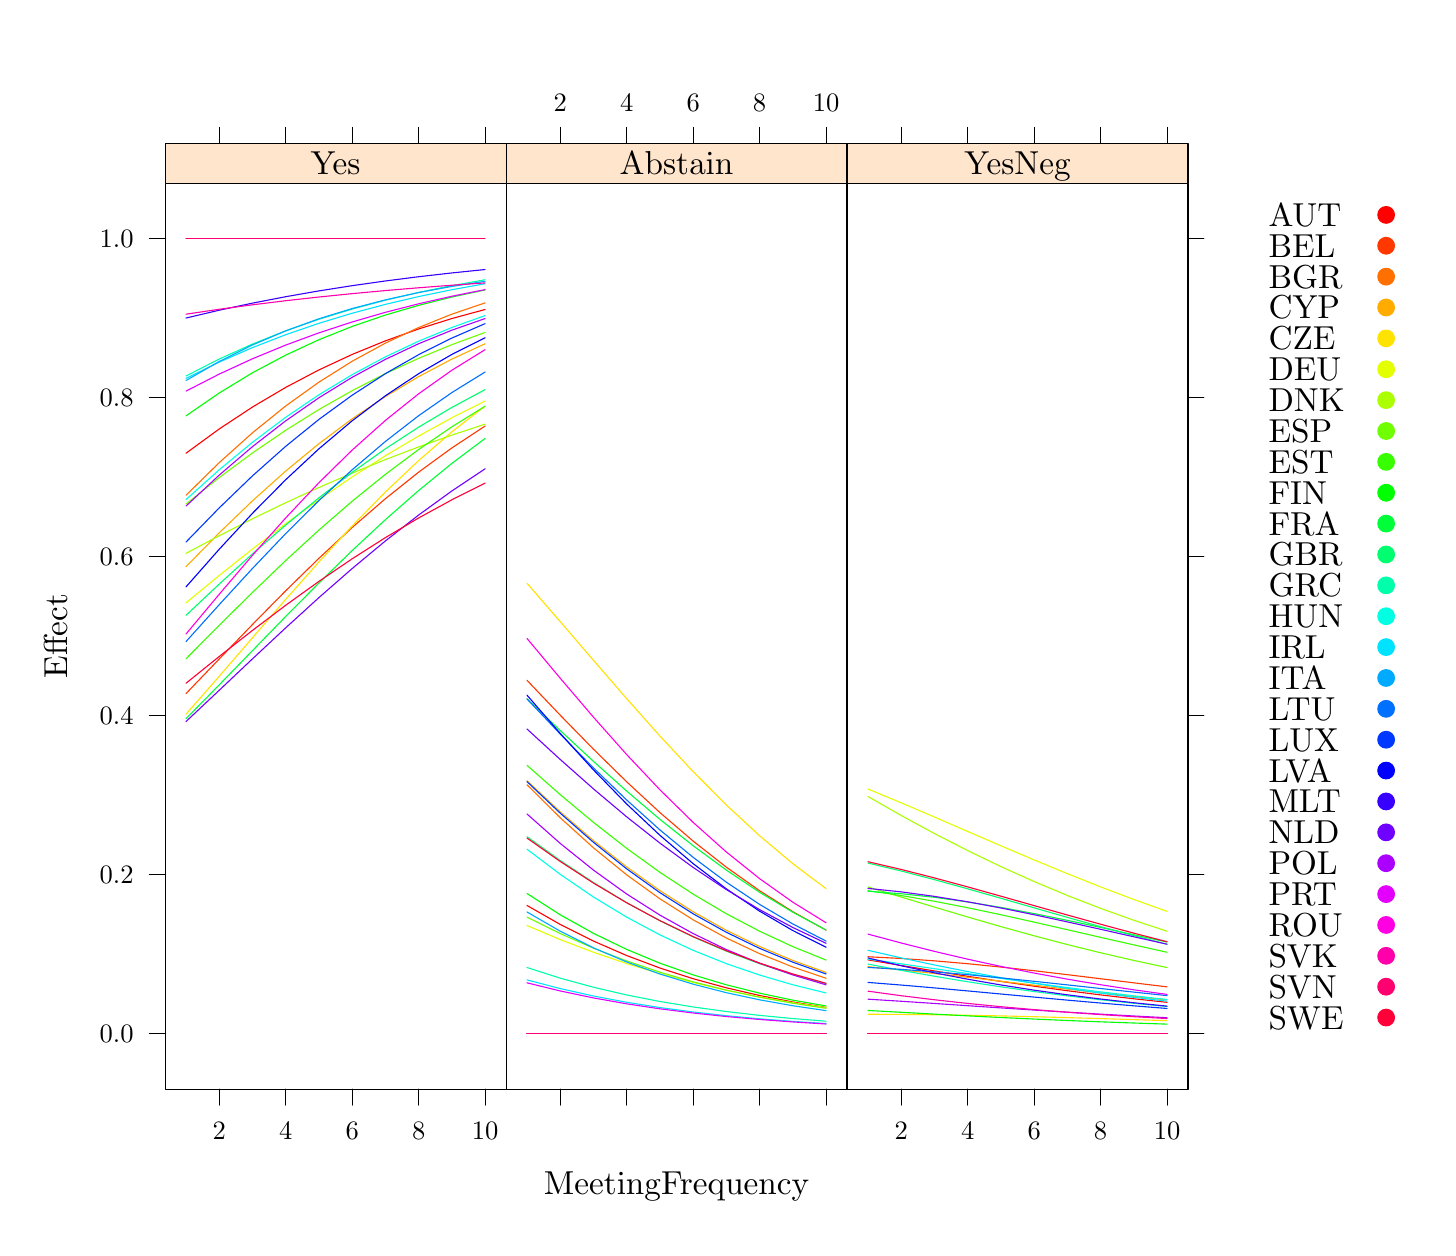
\begin{tikzpicture}[x=1pt,y=1pt]
\definecolor[named]{drawColor}{rgb}{0.00,0.00,0.00}
\definecolor[named]{fillColor}{rgb}{1.00,1.00,1.00}
\fill[color=fillColor,] (0,0) rectangle (505.89,433.62);
\begin{scope}
\path[clip] (  0.00,  0.00) rectangle (505.89,433.62);
\definecolor[named]{fillColor}{rgb}{0.00,0.00,0.00}
\end{scope}
\begin{scope}
\path[clip] (  0.00,  0.00) rectangle (505.89,433.62);
\definecolor[named]{fillColor}{rgb}{0.00,0.00,0.00}

\draw[fill opacity=0.00,draw opacity=0.00,] (  0.00,  0.00) rectangle (505.89,433.62);
\end{scope}
\begin{scope}
\path[clip] (  0.00,  0.00) rectangle (505.89,433.62);
\definecolor[named]{fillColor}{rgb}{0.00,0.00,0.00}
\end{scope}
\begin{scope}
\path[clip] (  0.00,  0.00) rectangle (505.89,433.62);
\definecolor[named]{fillColor}{rgb}{0.00,0.00,0.00}
\definecolor[named]{drawColor}{rgb}{0.00,0.00,0.00}

\node[color=drawColor,anchor=base,inner sep=0pt, outer sep=0pt, scale=  1.20] at (234.47, 12.04) {MeetingFrequency%
};
\end{scope}
\begin{scope}
\path[clip] (  0.00,  0.00) rectangle (505.89,433.62);
\definecolor[named]{fillColor}{rgb}{0.00,0.00,0.00}
\definecolor[named]{drawColor}{rgb}{0.00,0.00,0.00}

\node[rotate= 90.00,color=drawColor,anchor=base,inner sep=0pt, outer sep=0pt, scale=  1.20] at ( 14.29,213.72) {Effect%
};
\end{scope}
\begin{scope}
\path[clip] (  0.00,  0.00) rectangle (505.89,433.62);
\definecolor[named]{fillColor}{rgb}{0.00,0.00,0.00}
\end{scope}
\begin{scope}
\path[clip] (  0.00,  0.00) rectangle (505.89,433.62);
\definecolor[named]{fillColor}{rgb}{0.00,0.00,0.00}
\end{scope}
\begin{scope}
\path[clip] (  0.00,  0.00) rectangle (505.89,433.62);
\definecolor[named]{fillColor}{rgb}{0.00,0.00,0.00}
\end{scope}
\begin{scope}
\path[clip] ( 49.65, 50.02) rectangle (172.86,377.42);
\definecolor[named]{fillColor}{rgb}{0.00,0.00,0.00}
\end{scope}
\begin{scope}
\path[clip] (  0.00,  0.00) rectangle (505.89,433.62);
\definecolor[named]{fillColor}{rgb}{0.00,0.00,0.00}
\end{scope}
\begin{scope}
\path[clip] (  0.00,  0.00) rectangle (505.89,433.62);
\definecolor[named]{fillColor}{rgb}{0.00,0.00,0.00}
\definecolor[named]{drawColor}{rgb}{0.00,0.00,0.00}

\draw[color=drawColor,line cap=round,line join=round,fill opacity=0.00,] ( 69.22,391.87) -- ( 69.22,397.56);

\draw[color=drawColor,line cap=round,line join=round,fill opacity=0.00,] ( 93.24,391.87) -- ( 93.24,397.56);

\draw[color=drawColor,line cap=round,line join=round,fill opacity=0.00,] (117.26,391.87) -- (117.26,397.56);

\draw[color=drawColor,line cap=round,line join=round,fill opacity=0.00,] (141.28,391.87) -- (141.28,397.56);

\draw[color=drawColor,line cap=round,line join=round,fill opacity=0.00,] (165.29,391.87) -- (165.29,397.56);
\end{scope}
\begin{scope}
\path[clip] (  0.00,  0.00) rectangle (505.89,433.62);
\definecolor[named]{fillColor}{rgb}{0.00,0.00,0.00}
\end{scope}
\begin{scope}
\path[clip] (  0.00,  0.00) rectangle (505.89,433.62);
\definecolor[named]{fillColor}{rgb}{0.00,0.00,0.00}
\definecolor[named]{drawColor}{rgb}{0.00,0.00,0.00}

\draw[color=drawColor,line cap=round,line join=round,fill opacity=0.00,] ( 49.65, 70.12) -- ( 43.95, 70.12);

\draw[color=drawColor,line cap=round,line join=round,fill opacity=0.00,] ( 49.65,127.56) -- ( 43.95,127.56);

\draw[color=drawColor,line cap=round,line join=round,fill opacity=0.00,] ( 49.65,185.00) -- ( 43.95,185.00);

\draw[color=drawColor,line cap=round,line join=round,fill opacity=0.00,] ( 49.65,242.43) -- ( 43.95,242.43);

\draw[color=drawColor,line cap=round,line join=round,fill opacity=0.00,] ( 49.65,299.87) -- ( 43.95,299.87);

\draw[color=drawColor,line cap=round,line join=round,fill opacity=0.00,] ( 49.65,357.31) -- ( 43.95,357.31);

\node[color=drawColor,anchor=base east,inner sep=0pt, outer sep=0pt, scale=  0.96] at ( 38.26, 66.81) {0.0%
};

\node[color=drawColor,anchor=base east,inner sep=0pt, outer sep=0pt, scale=  0.96] at ( 38.26,124.25) {0.2%
};

\node[color=drawColor,anchor=base east,inner sep=0pt, outer sep=0pt, scale=  0.96] at ( 38.26,181.69) {0.4%
};

\node[color=drawColor,anchor=base east,inner sep=0pt, outer sep=0pt, scale=  0.96] at ( 38.26,239.13) {0.6%
};

\node[color=drawColor,anchor=base east,inner sep=0pt, outer sep=0pt, scale=  0.96] at ( 38.26,296.57) {0.8%
};

\node[color=drawColor,anchor=base east,inner sep=0pt, outer sep=0pt, scale=  0.96] at ( 38.26,354.01) {1.0%
};
\end{scope}
\begin{scope}
\path[clip] (  0.00,  0.00) rectangle (505.89,433.62);
\definecolor[named]{fillColor}{rgb}{0.00,0.00,0.00}
\end{scope}
\begin{scope}
\path[clip] (  0.00,  0.00) rectangle (505.89,433.62);
\definecolor[named]{fillColor}{rgb}{0.00,0.00,0.00}
\definecolor[named]{drawColor}{rgb}{0.00,0.00,0.00}

\draw[color=drawColor,line cap=round,line join=round,fill opacity=0.00,] ( 69.22, 50.02) -- ( 69.22, 44.32);

\draw[color=drawColor,line cap=round,line join=round,fill opacity=0.00,] ( 93.24, 50.02) -- ( 93.24, 44.32);

\draw[color=drawColor,line cap=round,line join=round,fill opacity=0.00,] (117.26, 50.02) -- (117.26, 44.32);

\draw[color=drawColor,line cap=round,line join=round,fill opacity=0.00,] (141.28, 50.02) -- (141.28, 44.32);

\draw[color=drawColor,line cap=round,line join=round,fill opacity=0.00,] (165.29, 50.02) -- (165.29, 44.32);

\node[color=drawColor,anchor=base,inner sep=0pt, outer sep=0pt, scale=  0.96] at ( 69.22, 32.02) {2%
};

\node[color=drawColor,anchor=base,inner sep=0pt, outer sep=0pt, scale=  0.96] at ( 93.24, 32.02) {4%
};

\node[color=drawColor,anchor=base,inner sep=0pt, outer sep=0pt, scale=  0.96] at (117.26, 32.02) {6%
};

\node[color=drawColor,anchor=base,inner sep=0pt, outer sep=0pt, scale=  0.96] at (141.28, 32.02) {8%
};

\node[color=drawColor,anchor=base,inner sep=0pt, outer sep=0pt, scale=  0.96] at (165.29, 32.02) {10%
};
\end{scope}
\begin{scope}
\path[clip] (  0.00,  0.00) rectangle (505.89,433.62);
\definecolor[named]{fillColor}{rgb}{0.00,0.00,0.00}
\end{scope}
\begin{scope}
\path[clip] ( 49.65, 50.02) rectangle (172.86,377.42);
\definecolor[named]{fillColor}{rgb}{0.00,0.00,0.00}
\definecolor[named]{drawColor}{rgb}{1.00,0.00,0.00}

\draw[color=drawColor,line cap=round,line join=round,fill opacity=0.00,] ( 57.21,279.84) --
	( 69.22,288.61) --
	( 81.23,296.53) --
	( 93.24,303.63) --
	(105.25,309.95) --
	(117.26,315.54) --
	(129.27,320.45) --
	(141.28,324.75) --
	(153.28,328.51) --
	(165.29,331.78);
\definecolor[named]{drawColor}{rgb}{1.00,0.22,0.00}

\draw[color=drawColor,line cap=round,line join=round,fill opacity=0.00,] ( 57.21,192.98) --
	( 69.22,205.49) --
	( 81.23,217.95) --
	( 93.24,230.14) --
	(105.25,241.88) --
	(117.26,253.01) --
	(129.27,263.41) --
	(141.28,273.01) --
	(153.28,281.76) --
	(165.29,289.67);
\definecolor[named]{drawColor}{rgb}{1.00,0.44,0.00}

\draw[color=drawColor,line cap=round,line join=round,fill opacity=0.00,] ( 57.21,264.63) --
	( 69.22,276.44) --
	( 81.23,287.22) --
	( 93.24,296.92) --
	(105.25,305.53) --
	(117.26,313.08) --
	(129.27,319.63) --
	(141.28,325.27) --
	(153.28,330.09) --
	(165.29,334.17);
\definecolor[named]{drawColor}{rgb}{1.00,0.67,0.00}

\draw[color=drawColor,line cap=round,line join=round,fill opacity=0.00,] ( 57.21,238.83) --
	( 69.22,251.07) --
	( 81.23,262.64) --
	( 93.24,273.40) --
	(105.25,283.30) --
	(117.26,292.28) --
	(129.27,300.34) --
	(141.28,307.52) --
	(153.28,313.85) --
	(165.29,319.40);
\definecolor[named]{drawColor}{rgb}{1.00,0.89,0.00}

\draw[color=drawColor,line cap=round,line join=round,fill opacity=0.00,] ( 57.21,185.54) --
	( 69.22,199.24) --
	( 81.23,213.15) --
	( 93.24,227.02) --
	(105.25,240.57) --
	(117.26,253.58) --
	(129.27,265.83) --
	(141.28,277.19) --
	(153.28,287.56) --
	(165.29,296.88);
\definecolor[named]{drawColor}{rgb}{0.89,1.00,0.00}

\draw[color=drawColor,line cap=round,line join=round,fill opacity=0.00,] ( 57.21,225.77) --
	( 69.22,235.67) --
	( 81.23,245.23) --
	( 93.24,254.39) --
	(105.25,263.08) --
	(117.26,271.27) --
	(129.27,278.94) --
	(141.28,286.06) --
	(153.28,292.64) --
	(165.29,298.69);
\definecolor[named]{drawColor}{rgb}{0.67,1.00,0.00}

\draw[color=drawColor,line cap=round,line join=round,fill opacity=0.00,] ( 57.21,243.66) --
	( 69.22,250.04) --
	( 81.23,256.15) --
	( 93.24,261.96) --
	(105.25,267.47) --
	(117.26,272.66) --
	(129.27,277.55) --
	(141.28,282.12) --
	(153.28,286.39) --
	(165.29,290.36);
\definecolor[named]{drawColor}{rgb}{0.44,1.00,0.00}

\draw[color=drawColor,line cap=round,line join=round,fill opacity=0.00,] ( 57.21,261.49) --
	( 69.22,271.05) --
	( 81.23,279.94) --
	( 93.24,288.14) --
	(105.25,295.64) --
	(117.26,302.45) --
	(129.27,308.61) --
	(141.28,314.14) --
	(153.28,319.08) --
	(165.29,323.49);
\definecolor[named]{drawColor}{rgb}{0.22,1.00,0.00}

\draw[color=drawColor,line cap=round,line join=round,fill opacity=0.00,] ( 57.21,205.56) --
	( 69.22,217.65) --
	( 81.23,229.54) --
	( 93.24,241.07) --
	(105.25,252.09) --
	(117.26,262.50) --
	(129.27,272.22) --
	(141.28,281.19) --
	(153.28,289.39) --
	(165.29,296.83);
\definecolor[named]{drawColor}{rgb}{0.00,1.00,0.00}

\draw[color=drawColor,line cap=round,line join=round,fill opacity=0.00,] ( 57.21,293.34) --
	( 69.22,301.61) --
	( 81.23,308.91) --
	( 93.24,315.30) --
	(105.25,320.86) --
	(117.26,325.66) --
	(129.27,329.77) --
	(141.28,333.29) --
	(153.28,336.30) --
	(165.29,338.85);
\definecolor[named]{drawColor}{rgb}{0.00,1.00,0.22}

\draw[color=drawColor,line cap=round,line join=round,fill opacity=0.00,] ( 57.21,183.92) --
	( 69.22,196.14) --
	( 81.23,208.51) --
	( 93.24,220.85) --
	(105.25,232.95) --
	(117.26,244.67) --
	(129.27,255.84) --
	(141.28,266.37) --
	(153.28,276.17) --
	(165.29,285.19);
\definecolor[named]{drawColor}{rgb}{0.00,1.00,0.44}

\draw[color=drawColor,line cap=round,line join=round,fill opacity=0.00,] ( 57.21,221.26) --
	( 69.22,232.56) --
	( 81.23,243.48) --
	( 93.24,253.90) --
	(105.25,263.75) --
	(117.26,272.94) --
	(129.27,281.45) --
	(141.28,289.27) --
	(153.28,296.39) --
	(165.29,302.84);
\definecolor[named]{drawColor}{rgb}{0.00,1.00,0.67}

\draw[color=drawColor,line cap=round,line join=round,fill opacity=0.00,] ( 57.21,307.77) --
	( 69.22,313.88) --
	( 81.23,319.29) --
	( 93.24,324.07) --
	(105.25,328.26) --
	(117.26,331.94) --
	(129.27,335.15) --
	(141.28,337.95) --
	(153.28,340.39) --
	(165.29,342.52);
\definecolor[named]{drawColor}{rgb}{0.00,1.00,0.89}

\draw[color=drawColor,line cap=round,line join=round,fill opacity=0.00,] ( 57.21,263.09) --
	( 69.22,273.86) --
	( 81.23,283.79) --
	( 93.24,292.83) --
	(105.25,300.97) --
	(117.26,308.23) --
	(129.27,314.67) --
	(141.28,320.33) --
	(153.28,325.28) --
	(165.29,329.58);
\definecolor[named]{drawColor}{rgb}{0.00,0.89,1.00}

\draw[color=drawColor,line cap=round,line join=round,fill opacity=0.00,] ( 57.21,306.90) --
	( 69.22,312.77) --
	( 81.23,318.01) --
	( 93.24,322.67) --
	(105.25,326.79) --
	(117.26,330.43) --
	(129.27,333.63) --
	(141.28,336.45) --
	(153.28,338.92) --
	(165.29,341.09);
\definecolor[named]{drawColor}{rgb}{0.00,0.67,1.00}

\draw[color=drawColor,line cap=round,line join=round,fill opacity=0.00,] ( 57.21,306.11) --
	( 69.22,312.99) --
	( 81.23,318.95) --
	( 93.24,324.06) --
	(105.25,328.43) --
	(117.26,332.13) --
	(129.27,335.26) --
	(141.28,337.90) --
	(153.28,340.11) --
	(165.29,341.98);
\definecolor[named]{drawColor}{rgb}{0.00,0.44,1.00}

\draw[color=drawColor,line cap=round,line join=round,fill opacity=0.00,] ( 57.21,211.77) --
	( 69.22,225.12) --
	( 81.23,238.20) --
	( 93.24,250.80) --
	(105.25,262.73) --
	(117.26,273.86) --
	(129.27,284.10) --
	(141.28,293.41) --
	(153.28,301.76) --
	(165.29,309.19);
\definecolor[named]{drawColor}{rgb}{0.00,0.22,1.00}

\draw[color=drawColor,line cap=round,line join=round,fill opacity=0.00,] ( 57.21,247.74) --
	( 69.22,260.09) --
	( 81.23,271.66) --
	( 93.24,282.34) --
	(105.25,292.07) --
	(117.26,300.81) --
	(129.27,308.60) --
	(141.28,315.46) --
	(153.28,321.46) --
	(165.29,326.67);
\definecolor[named]{drawColor}{rgb}{0.00,0.00,1.00}

\draw[color=drawColor,line cap=round,line join=round,fill opacity=0.00,] ( 57.21,231.54) --
	( 69.22,245.15) --
	( 81.23,258.13) --
	( 93.24,270.27) --
	(105.25,281.45) --
	(117.26,291.57) --
	(129.27,300.61) --
	(141.28,308.59) --
	(153.28,315.54) --
	(165.29,321.56);
\definecolor[named]{drawColor}{rgb}{0.22,0.00,1.00}

\draw[color=drawColor,line cap=round,line join=round,fill opacity=0.00,] ( 57.21,328.69) --
	( 69.22,331.52) --
	( 81.23,334.08) --
	( 93.24,336.40) --
	(105.25,338.50) --
	(117.26,340.39) --
	(129.27,342.09) --
	(141.28,343.62) --
	(153.28,344.99) --
	(165.29,346.22);
\definecolor[named]{drawColor}{rgb}{0.44,0.00,1.00}

\draw[color=drawColor,line cap=round,line join=round,fill opacity=0.00,] ( 57.21,182.88) --
	( 69.22,194.19) --
	( 81.23,205.54) --
	( 93.24,216.75) --
	(105.25,227.68) --
	(117.26,238.18) --
	(129.27,248.15) --
	(141.28,257.51) --
	(153.28,266.21) --
	(165.29,274.21);
\definecolor[named]{drawColor}{rgb}{0.67,0.00,1.00}

\draw[color=drawColor,line cap=round,line join=round,fill opacity=0.00,] ( 57.21,260.74) --
	( 69.22,271.95) --
	( 81.23,282.23) --
	( 93.24,291.55) --
	(105.25,299.89) --
	(117.26,307.28) --
	(129.27,313.76) --
	(141.28,319.41) --
	(153.28,324.30) --
	(165.29,328.51);
\definecolor[named]{drawColor}{rgb}{0.89,0.00,1.00}

\draw[color=drawColor,line cap=round,line join=round,fill opacity=0.00,] ( 57.21,302.28) --
	( 69.22,308.44) --
	( 81.23,313.97) --
	( 93.24,318.92) --
	(105.25,323.34) --
	(117.26,327.27) --
	(129.27,330.76) --
	(141.28,333.84) --
	(153.28,336.57) --
	(165.29,338.97);
\definecolor[named]{drawColor}{rgb}{1.00,0.00,0.89}

\draw[color=drawColor,line cap=round,line join=round,fill opacity=0.00,] ( 57.21,214.51) --
	( 69.22,228.88) --
	( 81.23,242.96) --
	( 93.24,256.47) --
	(105.25,269.20) --
	(117.26,280.98) --
	(129.27,291.70) --
	(141.28,301.32) --
	(153.28,309.83) --
	(165.29,317.27);
\definecolor[named]{drawColor}{rgb}{1.00,0.00,0.67}

\draw[color=drawColor,line cap=round,line join=round,fill opacity=0.00,] ( 57.21,330.08) --
	( 69.22,331.86) --
	( 81.23,333.48) --
	( 93.24,334.95) --
	(105.25,336.29) --
	(117.26,337.51) --
	(129.27,338.62) --
	(141.28,339.63) --
	(153.28,340.55) --
	(165.29,341.39);
\definecolor[named]{drawColor}{rgb}{1.00,0.00,0.44}

\draw[color=drawColor,line cap=round,line join=round,fill opacity=0.00,] ( 57.21,357.31) --
	( 69.22,357.31) --
	( 81.23,357.31) --
	( 93.24,357.31) --
	(105.25,357.31) --
	(117.26,357.31) --
	(129.27,357.31) --
	(141.28,357.31) --
	(153.28,357.31) --
	(165.29,357.31);
\definecolor[named]{drawColor}{rgb}{1.00,0.00,0.22}

\draw[color=drawColor,line cap=round,line join=round,fill opacity=0.00,] ( 57.21,196.72) --
	( 69.22,206.40) --
	( 81.23,215.82) --
	( 93.24,224.90) --
	(105.25,233.54) --
	(117.26,241.70) --
	(129.27,249.35) --
	(141.28,256.45) --
	(153.28,263.01) --
	(165.29,269.05);
\end{scope}
\begin{scope}
\path[clip] (  0.00,  0.00) rectangle (505.89,433.62);
\definecolor[named]{fillColor}{rgb}{0.00,0.00,0.00}
\end{scope}
\begin{scope}
\path[clip] (  0.00,  0.00) rectangle (505.89,433.62);
\definecolor[named]{fillColor}{rgb}{0.00,0.00,0.00}
\definecolor[named]{drawColor}{rgb}{0.00,0.00,0.00}

\draw[color=drawColor,line cap=round,line join=round,fill opacity=0.00,] ( 49.65, 50.02) rectangle (172.86,377.42);
\end{scope}
\begin{scope}
\path[clip] (  0.00,  0.00) rectangle (505.89,433.62);
\definecolor[named]{fillColor}{rgb}{0.00,0.00,0.00}
\end{scope}
\begin{scope}
\path[clip] (  0.00,  0.00) rectangle (505.89,433.62);
\definecolor[named]{fillColor}{rgb}{0.00,0.00,0.00}
\end{scope}
\begin{scope}
\path[clip] ( 49.65,377.42) rectangle (172.86,391.87);
\definecolor[named]{fillColor}{rgb}{0.00,0.00,0.00}
\definecolor[named]{drawColor}{rgb}{1.00,0.90,0.80}
\definecolor[named]{fillColor}{rgb}{1.00,0.90,0.80}

\draw[color=drawColor,line cap=round,line join=round,fill=fillColor,] ( 49.65,377.42) rectangle (172.86,391.87);
\definecolor[named]{drawColor}{rgb}{0.00,0.00,0.00}

\node[color=drawColor,anchor=base west,inner sep=0pt, outer sep=0pt, scale=  1.20] at (102.22,380.51) {Yes%
};
\end{scope}
\begin{scope}
\path[clip] (  0.00,  0.00) rectangle (505.89,433.62);
\definecolor[named]{fillColor}{rgb}{0.00,0.00,0.00}
\end{scope}
\begin{scope}
\path[clip] (  0.00,  0.00) rectangle (505.89,433.62);
\definecolor[named]{fillColor}{rgb}{0.00,0.00,0.00}
\definecolor[named]{drawColor}{rgb}{0.00,0.00,0.00}

\draw[color=drawColor,line cap=round,line join=round,fill opacity=0.00,] ( 49.65,377.42) rectangle (172.86,391.87);
\end{scope}
\begin{scope}
\path[clip] (  0.00,  0.00) rectangle (505.89,433.62);
\definecolor[named]{fillColor}{rgb}{0.00,0.00,0.00}
\end{scope}
\begin{scope}
\path[clip] (  0.00,  0.00) rectangle (505.89,433.62);
\definecolor[named]{fillColor}{rgb}{0.00,0.00,0.00}
\end{scope}
\begin{scope}
\path[clip] (172.86, 50.02) rectangle (296.07,377.42);
\definecolor[named]{fillColor}{rgb}{0.00,0.00,0.00}
\end{scope}
\begin{scope}
\path[clip] (  0.00,  0.00) rectangle (505.89,433.62);
\definecolor[named]{fillColor}{rgb}{0.00,0.00,0.00}
\end{scope}
\begin{scope}
\path[clip] (  0.00,  0.00) rectangle (505.89,433.62);
\definecolor[named]{fillColor}{rgb}{0.00,0.00,0.00}
\definecolor[named]{drawColor}{rgb}{0.00,0.00,0.00}

\draw[color=drawColor,line cap=round,line join=round,fill opacity=0.00,] (192.43,391.87) -- (192.43,397.56);

\draw[color=drawColor,line cap=round,line join=round,fill opacity=0.00,] (216.45,391.87) -- (216.45,397.56);

\draw[color=drawColor,line cap=round,line join=round,fill opacity=0.00,] (240.47,391.87) -- (240.47,397.56);

\draw[color=drawColor,line cap=round,line join=round,fill opacity=0.00,] (264.49,391.87) -- (264.49,397.56);

\draw[color=drawColor,line cap=round,line join=round,fill opacity=0.00,] (288.51,391.87) -- (288.51,397.56);

\node[color=drawColor,anchor=base,inner sep=0pt, outer sep=0pt, scale=  0.96] at (192.43,403.25) {2%
};

\node[color=drawColor,anchor=base,inner sep=0pt, outer sep=0pt, scale=  0.96] at (216.45,403.25) {4%
};

\node[color=drawColor,anchor=base,inner sep=0pt, outer sep=0pt, scale=  0.96] at (240.47,403.25) {6%
};

\node[color=drawColor,anchor=base,inner sep=0pt, outer sep=0pt, scale=  0.96] at (264.49,403.25) {8%
};

\node[color=drawColor,anchor=base,inner sep=0pt, outer sep=0pt, scale=  0.96] at (288.51,403.25) {10%
};
\end{scope}
\begin{scope}
\path[clip] (  0.00,  0.00) rectangle (505.89,433.62);
\definecolor[named]{fillColor}{rgb}{0.00,0.00,0.00}
\end{scope}
\begin{scope}
\path[clip] (  0.00,  0.00) rectangle (505.89,433.62);
\definecolor[named]{fillColor}{rgb}{0.00,0.00,0.00}
\end{scope}
\begin{scope}
\path[clip] (  0.00,  0.00) rectangle (505.89,433.62);
\definecolor[named]{fillColor}{rgb}{0.00,0.00,0.00}
\end{scope}
\begin{scope}
\path[clip] (  0.00,  0.00) rectangle (505.89,433.62);
\definecolor[named]{fillColor}{rgb}{0.00,0.00,0.00}
\definecolor[named]{drawColor}{rgb}{0.00,0.00,0.00}

\draw[color=drawColor,line cap=round,line join=round,fill opacity=0.00,] (192.43, 50.02) -- (192.43, 44.32);

\draw[color=drawColor,line cap=round,line join=round,fill opacity=0.00,] (216.45, 50.02) -- (216.45, 44.32);

\draw[color=drawColor,line cap=round,line join=round,fill opacity=0.00,] (240.47, 50.02) -- (240.47, 44.32);

\draw[color=drawColor,line cap=round,line join=round,fill opacity=0.00,] (264.49, 50.02) -- (264.49, 44.32);

\draw[color=drawColor,line cap=round,line join=round,fill opacity=0.00,] (288.51, 50.02) -- (288.51, 44.32);
\end{scope}
\begin{scope}
\path[clip] (  0.00,  0.00) rectangle (505.89,433.62);
\definecolor[named]{fillColor}{rgb}{0.00,0.00,0.00}
\end{scope}
\begin{scope}
\path[clip] (172.86, 50.02) rectangle (296.07,377.42);
\definecolor[named]{fillColor}{rgb}{0.00,0.00,0.00}
\definecolor[named]{drawColor}{rgb}{1.00,0.00,0.00}

\draw[color=drawColor,line cap=round,line join=round,fill opacity=0.00,] (180.42,116.43) --
	(192.43,109.58) --
	(204.44,103.57) --
	(216.45, 98.33) --
	(228.46, 93.82) --
	(240.47, 89.96) --
	(252.48, 86.67) --
	(264.49, 83.89) --
	(276.50, 81.55) --
	(288.51, 79.58);
\definecolor[named]{drawColor}{rgb}{1.00,0.22,0.00}

\draw[color=drawColor,line cap=round,line join=round,fill opacity=0.00,] (180.42,197.80) --
	(192.43,185.19) --
	(204.44,172.90) --
	(216.45,161.11) --
	(228.46,150.00) --
	(240.47,139.69) --
	(252.48,130.26) --
	(264.49,121.75) --
	(276.50,114.17) --
	(288.51,107.50);
\definecolor[named]{drawColor}{rgb}{1.00,0.44,0.00}

\draw[color=drawColor,line cap=round,line join=round,fill opacity=0.00,] (180.42,160.06) --
	(192.43,148.14) --
	(204.44,137.27) --
	(216.45,127.49) --
	(228.46,118.83) --
	(240.47,111.24) --
	(252.48,104.66) --
	(264.49, 99.01) --
	(276.50, 94.19) --
	(288.51, 90.12);
\definecolor[named]{drawColor}{rgb}{1.00,0.67,0.00}

\draw[color=drawColor,line cap=round,line join=round,fill opacity=0.00,] (180.42,161.49) --
	(192.43,150.27) --
	(204.44,139.87) --
	(216.45,130.36) --
	(228.46,121.79) --
	(240.47,114.16) --
	(252.48,107.45) --
	(264.49,101.60) --
	(276.50, 96.55) --
	(288.51, 92.23);
\definecolor[named]{drawColor}{rgb}{1.00,0.89,0.00}

\draw[color=drawColor,line cap=round,line join=round,fill opacity=0.00,] (180.42,232.85) --
	(192.43,219.01) --
	(204.44,205.02) --
	(216.45,191.16) --
	(228.46,177.67) --
	(240.47,164.80) --
	(252.48,152.73) --
	(264.49,141.61) --
	(276.50,131.52) --
	(288.51,122.49);
\definecolor[named]{drawColor}{rgb}{0.89,1.00,0.00}

\draw[color=drawColor,line cap=round,line join=round,fill opacity=0.00,] (180.42,109.19) --
	(192.43,104.11) --
	(204.44, 99.53) --
	(216.45, 95.43) --
	(228.46, 91.80) --
	(240.47, 88.60) --
	(252.48, 85.81) --
	(264.49, 83.39) --
	(276.50, 81.31) --
	(288.51, 79.52);
\definecolor[named]{drawColor}{rgb}{0.67,1.00,0.00}

\draw[color=drawColor,line cap=round,line join=round,fill opacity=0.00,] (180.42, 70.12) --
	(192.43, 70.12) --
	(204.44, 70.12) --
	(216.45, 70.12) --
	(228.46, 70.12) --
	(240.47, 70.12) --
	(252.48, 70.12) --
	(264.49, 70.12) --
	(276.50, 70.12) --
	(288.51, 70.12);
\definecolor[named]{drawColor}{rgb}{0.44,1.00,0.00}

\draw[color=drawColor,line cap=round,line join=round,fill opacity=0.00,] (180.42,112.21) --
	(192.43,106.27) --
	(204.44,100.99) --
	(216.45, 96.36) --
	(228.46, 92.32) --
	(240.47, 88.82) --
	(252.48, 85.82) --
	(264.49, 83.26) --
	(276.50, 81.09) --
	(288.51, 79.25);
\definecolor[named]{drawColor}{rgb}{0.22,1.00,0.00}

\draw[color=drawColor,line cap=round,line join=round,fill opacity=0.00,] (180.42,167.07) --
	(192.43,156.49) --
	(204.44,146.46) --
	(216.45,137.07) --
	(228.46,128.41) --
	(240.47,120.53) --
	(252.48,113.43) --
	(264.49,107.11) --
	(276.50,101.55) --
	(288.51, 96.70);
\definecolor[named]{drawColor}{rgb}{0.00,1.00,0.00}

\draw[color=drawColor,line cap=round,line join=round,fill opacity=0.00,] (180.42,120.76) --
	(192.43,113.07) --
	(204.44,106.36) --
	(216.45,100.55) --
	(228.46, 95.57) --
	(240.47, 91.34) --
	(252.48, 87.75) --
	(264.49, 84.74) --
	(276.50, 82.21) --
	(288.51, 80.11);
\definecolor[named]{drawColor}{rgb}{0.00,1.00,0.22}

\draw[color=drawColor,line cap=round,line join=round,fill opacity=0.00,] (180.42,191.05) --
	(192.43,179.65) --
	(204.44,168.50) --
	(216.45,157.76) --
	(228.46,147.55) --
	(240.47,138.01) --
	(252.48,129.20) --
	(264.49,121.18) --
	(276.50,113.97) --
	(288.51,107.56);
\definecolor[named]{drawColor}{rgb}{0.00,1.00,0.44}

\draw[color=drawColor,line cap=round,line join=round,fill opacity=0.00,] (180.42,141.27) --
	(192.43,132.67) --
	(204.44,124.72) --
	(216.45,117.46) --
	(228.46,110.91) --
	(240.47,105.07) --
	(252.48, 99.90) --
	(264.49, 95.38) --
	(276.50, 91.45) --
	(288.51, 88.06);
\definecolor[named]{drawColor}{rgb}{0.00,1.00,0.67}

\draw[color=drawColor,line cap=round,line join=round,fill opacity=0.00,] (180.42, 94.01) --
	(192.43, 90.16) --
	(204.44, 86.88) --
	(216.45, 84.09) --
	(228.46, 81.73) --
	(240.47, 79.75) --
	(252.48, 78.10) --
	(264.49, 76.71) --
	(276.50, 75.56) --
	(288.51, 74.61);
\definecolor[named]{drawColor}{rgb}{0.00,1.00,0.89}

\draw[color=drawColor,line cap=round,line join=round,fill opacity=0.00,] (180.42,136.77) --
	(192.43,127.68) --
	(204.44,119.49) --
	(216.45,112.21) --
	(228.46,105.80) --
	(240.47,100.22) --
	(252.48, 95.41) --
	(264.49, 91.28) --
	(276.50, 87.77) --
	(288.51, 84.80);
\definecolor[named]{drawColor}{rgb}{0.00,0.89,1.00}

\draw[color=drawColor,line cap=round,line join=round,fill opacity=0.00,] (180.42, 89.54) --
	(192.43, 86.40) --
	(204.44, 83.72) --
	(216.45, 81.45) --
	(228.46, 79.54) --
	(240.47, 77.94) --
	(252.48, 76.59) --
	(264.49, 75.47) --
	(276.50, 74.54) --
	(288.51, 73.76);
\definecolor[named]{drawColor}{rgb}{0.00,0.67,1.00}

\draw[color=drawColor,line cap=round,line join=round,fill opacity=0.00,] (180.42,114.08) --
	(192.43,107.13) --
	(204.44,101.13) --
	(216.45, 96.00) --
	(228.46, 91.65) --
	(240.47, 87.99) --
	(252.48, 84.91) --
	(264.49, 82.33) --
	(276.50, 80.19) --
	(288.51, 78.42);
\definecolor[named]{drawColor}{rgb}{0.00,0.44,1.00}

\draw[color=drawColor,line cap=round,line join=round,fill opacity=0.00,] (180.42,191.08) --
	(192.43,178.38) --
	(204.44,166.14) --
	(216.45,154.54) --
	(228.46,143.73) --
	(240.47,133.81) --
	(252.48,124.83) --
	(264.49,116.81) --
	(276.50,109.74) --
	(288.51,103.56);
\definecolor[named]{drawColor}{rgb}{0.00,0.22,1.00}

\draw[color=drawColor,line cap=round,line join=round,fill opacity=0.00,] (180.42,161.19) --
	(192.43,149.79) --
	(204.44,139.25) --
	(216.45,129.66) --
	(228.46,121.05) --
	(240.47,113.42) --
	(252.48,106.73) --
	(264.49,100.92) --
	(276.50, 95.93) --
	(288.51, 91.67);
\definecolor[named]{drawColor}{rgb}{0.00,0.00,1.00}

\draw[color=drawColor,line cap=round,line join=round,fill opacity=0.00,] (180.42,192.43) --
	(192.43,178.60) --
	(204.44,165.42) --
	(216.45,153.10) --
	(228.46,141.78) --
	(240.47,131.54) --
	(252.48,122.41) --
	(264.49,114.36) --
	(276.50,107.36) --
	(288.51,101.33);
\definecolor[named]{drawColor}{rgb}{0.22,0.00,1.00}

\draw[color=drawColor,line cap=round,line join=round,fill opacity=0.00,] (180.42, 70.12) --
	(192.43, 70.12) --
	(204.44, 70.12) --
	(216.45, 70.12) --
	(228.46, 70.12) --
	(240.47, 70.12) --
	(252.48, 70.12) --
	(264.49, 70.12) --
	(276.50, 70.12) --
	(288.51, 70.12);
\definecolor[named]{drawColor}{rgb}{0.44,0.00,1.00}

\draw[color=drawColor,line cap=round,line join=round,fill opacity=0.00,] (180.42,180.20) --
	(192.43,169.19) --
	(204.44,158.56) --
	(216.45,148.45) --
	(228.46,138.96) --
	(240.47,130.17) --
	(252.48,122.15) --
	(264.49,114.92) --
	(276.50,108.46) --
	(288.51,102.76);
\definecolor[named]{drawColor}{rgb}{0.67,0.00,1.00}

\draw[color=drawColor,line cap=round,line join=round,fill opacity=0.00,] (180.42,149.49) --
	(192.43,138.86) --
	(204.44,129.21) --
	(216.45,120.57) --
	(228.46,112.94) --
	(240.47,106.27) --
	(252.48,100.49) --
	(264.49, 95.54) --
	(276.50, 91.32) --
	(288.51, 87.74);
\definecolor[named]{drawColor}{rgb}{0.89,0.00,1.00}

\draw[color=drawColor,line cap=round,line join=round,fill opacity=0.00,] (180.42, 88.48) --
	(192.43, 85.54) --
	(204.44, 83.02) --
	(216.45, 80.89) --
	(228.46, 79.08) --
	(240.47, 77.57) --
	(252.48, 76.29) --
	(264.49, 75.23) --
	(276.50, 74.34) --
	(288.51, 73.60);
\definecolor[named]{drawColor}{rgb}{1.00,0.00,0.89}

\draw[color=drawColor,line cap=round,line join=round,fill opacity=0.00,] (180.42,212.92) --
	(192.43,198.55) --
	(204.44,184.47) --
	(216.45,170.96) --
	(228.46,158.23) --
	(240.47,146.45) --
	(252.48,135.73) --
	(264.49,126.11) --
	(276.50,117.60) --
	(288.51,110.16);
\definecolor[named]{drawColor}{rgb}{1.00,0.00,0.67}

\draw[color=drawColor,line cap=round,line join=round,fill opacity=0.00,] (180.42, 70.12) --
	(192.43, 70.12) --
	(204.44, 70.12) --
	(216.45, 70.12) --
	(228.46, 70.12) --
	(240.47, 70.12) --
	(252.48, 70.12) --
	(264.49, 70.12) --
	(276.50, 70.12) --
	(288.51, 70.12);
\definecolor[named]{drawColor}{rgb}{1.00,0.00,0.44}

\draw[color=drawColor,line cap=round,line join=round,fill opacity=0.00,] (180.42, 70.12) --
	(192.43, 70.12) --
	(204.44, 70.12) --
	(216.45, 70.12) --
	(228.46, 70.12) --
	(240.47, 70.12) --
	(252.48, 70.12) --
	(264.49, 70.12) --
	(276.50, 70.12) --
	(288.51, 70.12);
\definecolor[named]{drawColor}{rgb}{1.00,0.00,0.22}

\draw[color=drawColor,line cap=round,line join=round,fill opacity=0.00,] (180.42,140.79) --
	(192.43,132.34) --
	(204.44,124.53) --
	(216.45,117.39) --
	(228.46,110.95) --
	(240.47,105.18) --
	(252.48,100.07) --
	(264.49, 95.59) --
	(276.50, 91.68) --
	(288.51, 88.31);
\end{scope}
\begin{scope}
\path[clip] (  0.00,  0.00) rectangle (505.89,433.62);
\definecolor[named]{fillColor}{rgb}{0.00,0.00,0.00}
\end{scope}
\begin{scope}
\path[clip] (  0.00,  0.00) rectangle (505.89,433.62);
\definecolor[named]{fillColor}{rgb}{0.00,0.00,0.00}
\definecolor[named]{drawColor}{rgb}{0.00,0.00,0.00}

\draw[color=drawColor,line cap=round,line join=round,fill opacity=0.00,] (172.86, 50.02) rectangle (296.07,377.42);
\end{scope}
\begin{scope}
\path[clip] (  0.00,  0.00) rectangle (505.89,433.62);
\definecolor[named]{fillColor}{rgb}{0.00,0.00,0.00}
\end{scope}
\begin{scope}
\path[clip] (  0.00,  0.00) rectangle (505.89,433.62);
\definecolor[named]{fillColor}{rgb}{0.00,0.00,0.00}
\end{scope}
\begin{scope}
\path[clip] (172.86,377.42) rectangle (296.07,391.87);
\definecolor[named]{fillColor}{rgb}{0.00,0.00,0.00}
\definecolor[named]{drawColor}{rgb}{1.00,0.90,0.80}
\definecolor[named]{fillColor}{rgb}{1.00,0.90,0.80}

\draw[color=drawColor,line cap=round,line join=round,fill=fillColor,] (172.86,377.42) rectangle (296.07,391.87);
\definecolor[named]{drawColor}{rgb}{0.00,0.00,0.00}

\node[color=drawColor,anchor=base west,inner sep=0pt, outer sep=0pt, scale=  1.20] at (213.94,380.51) {Abstain%
};
\end{scope}
\begin{scope}
\path[clip] (  0.00,  0.00) rectangle (505.89,433.62);
\definecolor[named]{fillColor}{rgb}{0.00,0.00,0.00}
\end{scope}
\begin{scope}
\path[clip] (  0.00,  0.00) rectangle (505.89,433.62);
\definecolor[named]{fillColor}{rgb}{0.00,0.00,0.00}
\definecolor[named]{drawColor}{rgb}{0.00,0.00,0.00}

\draw[color=drawColor,line cap=round,line join=round,fill opacity=0.00,] (172.86,377.42) rectangle (296.07,391.87);
\end{scope}
\begin{scope}
\path[clip] (  0.00,  0.00) rectangle (505.89,433.62);
\definecolor[named]{fillColor}{rgb}{0.00,0.00,0.00}
\end{scope}
\begin{scope}
\path[clip] (  0.00,  0.00) rectangle (505.89,433.62);
\definecolor[named]{fillColor}{rgb}{0.00,0.00,0.00}
\end{scope}
\begin{scope}
\path[clip] (296.07, 50.02) rectangle (419.29,377.42);
\definecolor[named]{fillColor}{rgb}{0.00,0.00,0.00}
\end{scope}
\begin{scope}
\path[clip] (  0.00,  0.00) rectangle (505.89,433.62);
\definecolor[named]{fillColor}{rgb}{0.00,0.00,0.00}
\end{scope}
\begin{scope}
\path[clip] (  0.00,  0.00) rectangle (505.89,433.62);
\definecolor[named]{fillColor}{rgb}{0.00,0.00,0.00}
\definecolor[named]{drawColor}{rgb}{0.00,0.00,0.00}

\draw[color=drawColor,line cap=round,line join=round,fill opacity=0.00,] (315.65,391.87) -- (315.65,397.56);

\draw[color=drawColor,line cap=round,line join=round,fill opacity=0.00,] (339.67,391.87) -- (339.67,397.56);

\draw[color=drawColor,line cap=round,line join=round,fill opacity=0.00,] (363.69,391.87) -- (363.69,397.56);

\draw[color=drawColor,line cap=round,line join=round,fill opacity=0.00,] (387.70,391.87) -- (387.70,397.56);

\draw[color=drawColor,line cap=round,line join=round,fill opacity=0.00,] (411.72,391.87) -- (411.72,397.56);
\end{scope}
\begin{scope}
\path[clip] (  0.00,  0.00) rectangle (505.89,433.62);
\definecolor[named]{fillColor}{rgb}{0.00,0.00,0.00}
\end{scope}
\begin{scope}
\path[clip] (  0.00,  0.00) rectangle (505.89,433.62);
\definecolor[named]{fillColor}{rgb}{0.00,0.00,0.00}
\end{scope}
\begin{scope}
\path[clip] (  0.00,  0.00) rectangle (505.89,433.62);
\definecolor[named]{fillColor}{rgb}{0.00,0.00,0.00}
\end{scope}
\begin{scope}
\path[clip] (  0.00,  0.00) rectangle (505.89,433.62);
\definecolor[named]{fillColor}{rgb}{0.00,0.00,0.00}
\definecolor[named]{drawColor}{rgb}{0.00,0.00,0.00}

\draw[color=drawColor,line cap=round,line join=round,fill opacity=0.00,] (315.65, 50.02) -- (315.65, 44.32);

\draw[color=drawColor,line cap=round,line join=round,fill opacity=0.00,] (339.67, 50.02) -- (339.67, 44.32);

\draw[color=drawColor,line cap=round,line join=round,fill opacity=0.00,] (363.69, 50.02) -- (363.69, 44.32);

\draw[color=drawColor,line cap=round,line join=round,fill opacity=0.00,] (387.70, 50.02) -- (387.70, 44.32);

\draw[color=drawColor,line cap=round,line join=round,fill opacity=0.00,] (411.72, 50.02) -- (411.72, 44.32);

\node[color=drawColor,anchor=base,inner sep=0pt, outer sep=0pt, scale=  0.96] at (315.65, 32.02) {2%
};

\node[color=drawColor,anchor=base,inner sep=0pt, outer sep=0pt, scale=  0.96] at (339.67, 32.02) {4%
};

\node[color=drawColor,anchor=base,inner sep=0pt, outer sep=0pt, scale=  0.96] at (363.69, 32.02) {6%
};

\node[color=drawColor,anchor=base,inner sep=0pt, outer sep=0pt, scale=  0.96] at (387.70, 32.02) {8%
};

\node[color=drawColor,anchor=base,inner sep=0pt, outer sep=0pt, scale=  0.96] at (411.72, 32.02) {10%
};

\draw[color=drawColor,line cap=round,line join=round,fill opacity=0.00,] (419.29, 70.12) -- (424.98, 70.12);

\draw[color=drawColor,line cap=round,line join=round,fill opacity=0.00,] (419.29,127.56) -- (424.98,127.56);

\draw[color=drawColor,line cap=round,line join=round,fill opacity=0.00,] (419.29,185.00) -- (424.98,185.00);

\draw[color=drawColor,line cap=round,line join=round,fill opacity=0.00,] (419.29,242.43) -- (424.98,242.43);

\draw[color=drawColor,line cap=round,line join=round,fill opacity=0.00,] (419.29,299.87) -- (424.98,299.87);

\draw[color=drawColor,line cap=round,line join=round,fill opacity=0.00,] (419.29,357.31) -- (424.98,357.31);
\end{scope}
\begin{scope}
\path[clip] (  0.00,  0.00) rectangle (505.89,433.62);
\definecolor[named]{fillColor}{rgb}{0.00,0.00,0.00}
\end{scope}
\begin{scope}
\path[clip] (296.07, 50.02) rectangle (419.29,377.42);
\definecolor[named]{fillColor}{rgb}{0.00,0.00,0.00}
\definecolor[named]{drawColor}{rgb}{1.00,0.00,0.00}

\draw[color=drawColor,line cap=round,line join=round,fill opacity=0.00,] (303.64, 96.77) --
	(315.65, 94.75) --
	(327.66, 92.76) --
	(339.67, 90.83) --
	(351.68, 88.99) --
	(363.69, 87.25) --
	(375.69, 85.62) --
	(387.70, 84.11) --
	(399.71, 82.71) --
	(411.72, 81.43);
\definecolor[named]{drawColor}{rgb}{1.00,0.22,0.00}

\draw[color=drawColor,line cap=round,line join=round,fill opacity=0.00,] (303.64, 97.90) --
	(315.65, 97.27) --
	(327.66, 96.42) --
	(339.67, 95.38) --
	(351.68, 94.17) --
	(363.69, 92.84) --
	(375.69, 91.42) --
	(387.70, 89.95) --
	(399.71, 88.47) --
	(411.72, 87.01);
\definecolor[named]{drawColor}{rgb}{1.00,0.44,0.00}

\draw[color=drawColor,line cap=round,line join=round,fill opacity=0.00,] (303.64, 70.12) --
	(315.65, 70.12) --
	(327.66, 70.12) --
	(339.67, 70.12) --
	(351.68, 70.12) --
	(363.69, 70.12) --
	(375.69, 70.12) --
	(387.70, 70.12) --
	(399.71, 70.12) --
	(411.72, 70.12);
\definecolor[named]{drawColor}{rgb}{1.00,0.67,0.00}

\draw[color=drawColor,line cap=round,line join=round,fill opacity=0.00,] (303.64, 94.31) --
	(315.65, 93.14) --
	(327.66, 91.84) --
	(339.67, 90.47) --
	(351.68, 89.05) --
	(363.69, 87.62) --
	(375.69, 86.21) --
	(387.70, 84.84) --
	(399.71, 83.52) --
	(411.72, 82.28);
\definecolor[named]{drawColor}{rgb}{1.00,0.89,0.00}

\draw[color=drawColor,line cap=round,line join=round,fill opacity=0.00,] (303.64, 77.12) --
	(315.65, 77.06) --
	(327.66, 76.94) --
	(339.67, 76.76) --
	(351.68, 76.52) --
	(363.69, 76.23) --
	(375.69, 75.90) --
	(387.70, 75.55) --
	(399.71, 75.17) --
	(411.72, 74.80);
\definecolor[named]{drawColor}{rgb}{0.89,1.00,0.00}

\draw[color=drawColor,line cap=round,line join=round,fill opacity=0.00,] (303.64,158.51) --
	(315.65,153.52) --
	(327.66,148.38) --
	(339.67,143.17) --
	(351.68,137.99) --
	(363.69,132.88) --
	(375.69,127.92) --
	(387.70,123.14) --
	(399.71,118.59) --
	(411.72,114.29);
\definecolor[named]{drawColor}{rgb}{0.67,1.00,0.00}

\draw[color=drawColor,line cap=round,line join=round,fill opacity=0.00,] (303.64,155.81) --
	(315.65,148.94) --
	(327.66,142.41) --
	(339.67,136.25) --
	(351.68,130.47) --
	(363.69,125.07) --
	(375.69,120.04) --
	(387.70,115.38) --
	(399.71,111.08) --
	(411.72,107.12);
\definecolor[named]{drawColor}{rgb}{0.44,1.00,0.00}

\draw[color=drawColor,line cap=round,line join=round,fill opacity=0.00,] (303.64,123.11) --
	(315.65,119.47) --
	(327.66,115.84) --
	(339.67,112.26) --
	(351.68,108.79) --
	(363.69,105.46) --
	(375.69,102.30) --
	(387.70, 99.33) --
	(399.71, 96.56) --
	(411.72, 93.99);
\definecolor[named]{drawColor}{rgb}{0.22,1.00,0.00}

\draw[color=drawColor,line cap=round,line join=round,fill opacity=0.00,] (303.64,121.75) --
	(315.65,120.01) --
	(327.66,117.94) --
	(339.67,115.61) --
	(351.68,113.08) --
	(363.69,110.41) --
	(375.69,107.67) --
	(387.70,104.90) --
	(399.71,102.18) --
	(411.72, 99.52);
\definecolor[named]{drawColor}{rgb}{0.00,1.00,0.00}

\draw[color=drawColor,line cap=round,line join=round,fill opacity=0.00,] (303.64, 78.49) --
	(315.65, 77.82) --
	(327.66, 77.16) --
	(339.67, 76.54) --
	(351.68, 75.94) --
	(363.69, 75.38) --
	(375.69, 74.86) --
	(387.70, 74.38) --
	(399.71, 73.95) --
	(411.72, 73.55);
\definecolor[named]{drawColor}{rgb}{0.00,1.00,0.22}

\draw[color=drawColor,line cap=round,line join=round,fill opacity=0.00,] (303.64,121.58) --
	(315.65,120.67) --
	(327.66,119.37) --
	(339.67,117.70) --
	(351.68,115.72) --
	(363.69,113.48) --
	(375.69,111.05) --
	(387.70,108.49) --
	(399.71,105.85) --
	(411.72,103.21);
\definecolor[named]{drawColor}{rgb}{0.00,1.00,0.44}

\draw[color=drawColor,line cap=round,line join=round,fill opacity=0.00,] (303.64,131.75) --
	(315.65,128.88) --
	(327.66,125.75) --
	(339.67,122.44) --
	(351.68,119.02) --
	(363.69,115.56) --
	(375.69,112.12) --
	(387.70,108.75) --
	(399.71,105.51) --
	(411.72,102.41);
\definecolor[named]{drawColor}{rgb}{0.00,1.00,0.67}

\draw[color=drawColor,line cap=round,line join=round,fill opacity=0.00,] (303.64, 95.24) --
	(315.65, 92.98) --
	(327.66, 90.85) --
	(339.67, 88.86) --
	(351.68, 87.02) --
	(363.69, 85.32) --
	(375.69, 83.77) --
	(387.70, 82.36) --
	(399.71, 81.08) --
	(411.72, 79.92);
\definecolor[named]{drawColor}{rgb}{0.00,1.00,0.89}

\draw[color=drawColor,line cap=round,line join=round,fill opacity=0.00,] (303.64, 97.05) --
	(315.65, 95.34) --
	(327.66, 93.58) --
	(339.67, 91.81) --
	(351.68, 90.07) --
	(363.69, 88.37) --
	(375.69, 86.75) --
	(387.70, 85.21) --
	(399.71, 83.77) --
	(411.72, 82.44);
\definecolor[named]{drawColor}{rgb}{0.00,0.89,1.00}

\draw[color=drawColor,line cap=round,line join=round,fill opacity=0.00,] (303.64,100.23) --
	(315.65, 97.49) --
	(327.66, 94.93) --
	(339.67, 92.54) --
	(351.68, 90.33) --
	(363.69, 88.31) --
	(375.69, 86.45) --
	(387.70, 84.76) --
	(399.71, 83.23) --
	(411.72, 81.84);
\definecolor[named]{drawColor}{rgb}{0.00,0.67,1.00}

\draw[color=drawColor,line cap=round,line join=round,fill opacity=0.00,] (303.64, 70.12) --
	(315.65, 70.12) --
	(327.66, 70.12) --
	(339.67, 70.12) --
	(351.68, 70.12) --
	(363.69, 70.12) --
	(375.69, 70.12) --
	(387.70, 70.12) --
	(399.71, 70.12) --
	(411.72, 70.12);
\definecolor[named]{drawColor}{rgb}{0.00,0.44,1.00}

\draw[color=drawColor,line cap=round,line join=round,fill opacity=0.00,] (303.64, 94.04) --
	(315.65, 93.34) --
	(327.66, 92.45) --
	(339.67, 91.42) --
	(351.68, 90.26) --
	(363.69, 89.02) --
	(375.69, 87.73) --
	(387.70, 86.42) --
	(399.71, 85.12) --
	(411.72, 83.85);
\definecolor[named]{drawColor}{rgb}{0.00,0.22,1.00}

\draw[color=drawColor,line cap=round,line join=round,fill opacity=0.00,] (303.64, 88.62) --
	(315.65, 87.67) --
	(327.66, 86.64) --
	(339.67, 85.55) --
	(351.68, 84.43) --
	(363.69, 83.32) --
	(375.69, 82.22) --
	(387.70, 81.17) --
	(399.71, 80.16) --
	(411.72, 79.21);
\definecolor[named]{drawColor}{rgb}{0.00,0.00,1.00}

\draw[color=drawColor,line cap=round,line join=round,fill opacity=0.00,] (303.64, 70.12) --
	(315.65, 70.12) --
	(327.66, 70.12) --
	(339.67, 70.12) --
	(351.68, 70.12) --
	(363.69, 70.12) --
	(375.69, 70.12) --
	(387.70, 70.12) --
	(399.71, 70.12) --
	(411.72, 70.12);
\definecolor[named]{drawColor}{rgb}{0.22,0.00,1.00}

\draw[color=drawColor,line cap=round,line join=round,fill opacity=0.00,] (303.64, 97.46) --
	(315.65, 94.64) --
	(327.66, 92.09) --
	(339.67, 89.78) --
	(351.68, 87.70) --
	(363.69, 85.82) --
	(375.69, 84.14) --
	(387.70, 82.62) --
	(399.71, 81.27) --
	(411.72, 80.05);
\definecolor[named]{drawColor}{rgb}{0.44,0.00,1.00}

\draw[color=drawColor,line cap=round,line join=round,fill opacity=0.00,] (303.64,122.59) --
	(315.65,121.34) --
	(327.66,119.71) --
	(339.67,117.75) --
	(351.68,115.52) --
	(363.69,113.08) --
	(375.69,110.49) --
	(387.70,107.82) --
	(399.71,105.11) --
	(411.72,102.43);
\definecolor[named]{drawColor}{rgb}{0.67,0.00,1.00}

\draw[color=drawColor,line cap=round,line join=round,fill opacity=0.00,] (303.64, 82.57) --
	(315.65, 81.81) --
	(327.66, 81.02) --
	(339.67, 80.21) --
	(351.68, 79.41) --
	(363.69, 78.63) --
	(375.69, 77.87) --
	(387.70, 77.16) --
	(399.71, 76.49) --
	(411.72, 75.86);
\definecolor[named]{drawColor}{rgb}{0.89,0.00,1.00}

\draw[color=drawColor,line cap=round,line join=round,fill opacity=0.00,] (303.64,106.08) --
	(315.65,102.87) --
	(327.66, 99.84) --
	(339.67, 97.02) --
	(351.68, 94.41) --
	(363.69, 92.00) --
	(375.69, 89.80) --
	(387.70, 87.78) --
	(399.71, 85.95) --
	(411.72, 84.29);
\definecolor[named]{drawColor}{rgb}{1.00,0.00,0.89}

\draw[color=drawColor,line cap=round,line join=round,fill opacity=0.00,] (303.64, 70.12) --
	(315.65, 70.12) --
	(327.66, 70.12) --
	(339.67, 70.12) --
	(351.68, 70.12) --
	(363.69, 70.12) --
	(375.69, 70.12) --
	(387.70, 70.12) --
	(399.71, 70.12) --
	(411.72, 70.12);
\definecolor[named]{drawColor}{rgb}{1.00,0.00,0.67}

\draw[color=drawColor,line cap=round,line join=round,fill opacity=0.00,] (303.64, 85.46) --
	(315.65, 83.82) --
	(327.66, 82.35) --
	(339.67, 81.03) --
	(351.68, 79.85) --
	(363.69, 78.79) --
	(375.69, 77.84) --
	(387.70, 77.00) --
	(399.71, 76.24) --
	(411.72, 75.57);
\definecolor[named]{drawColor}{rgb}{1.00,0.00,0.44}

\draw[color=drawColor,line cap=round,line join=round,fill opacity=0.00,] (303.64, 70.12) --
	(315.65, 70.12) --
	(327.66, 70.12) --
	(339.67, 70.12) --
	(351.68, 70.12) --
	(363.69, 70.12) --
	(375.69, 70.12) --
	(387.70, 70.12) --
	(399.71, 70.12) --
	(411.72, 70.12);
\definecolor[named]{drawColor}{rgb}{1.00,0.00,0.22}

\draw[color=drawColor,line cap=round,line join=round,fill opacity=0.00,] (303.64,132.24) --
	(315.65,129.44) --
	(327.66,126.38) --
	(339.67,123.14) --
	(351.68,119.78) --
	(363.69,116.37) --
	(375.69,112.98) --
	(387.70,109.65) --
	(399.71,106.42) --
	(411.72,103.33);
\end{scope}
\begin{scope}
\path[clip] (  0.00,  0.00) rectangle (505.89,433.62);
\definecolor[named]{fillColor}{rgb}{0.00,0.00,0.00}
\end{scope}
\begin{scope}
\path[clip] (  0.00,  0.00) rectangle (505.89,433.62);
\definecolor[named]{fillColor}{rgb}{0.00,0.00,0.00}
\definecolor[named]{drawColor}{rgb}{0.00,0.00,0.00}

\draw[color=drawColor,line cap=round,line join=round,fill opacity=0.00,] (296.07, 50.02) rectangle (419.29,377.42);
\end{scope}
\begin{scope}
\path[clip] (  0.00,  0.00) rectangle (505.89,433.62);
\definecolor[named]{fillColor}{rgb}{0.00,0.00,0.00}
\end{scope}
\begin{scope}
\path[clip] (  0.00,  0.00) rectangle (505.89,433.62);
\definecolor[named]{fillColor}{rgb}{0.00,0.00,0.00}
\end{scope}
\begin{scope}
\path[clip] (296.07,377.42) rectangle (419.29,391.87);
\definecolor[named]{fillColor}{rgb}{0.00,0.00,0.00}
\definecolor[named]{drawColor}{rgb}{1.00,0.90,0.80}
\definecolor[named]{fillColor}{rgb}{1.00,0.90,0.80}

\draw[color=drawColor,line cap=round,line join=round,fill=fillColor,] (296.07,377.42) rectangle (419.29,391.87);
\definecolor[named]{drawColor}{rgb}{0.00,0.00,0.00}

\node[color=drawColor,anchor=base west,inner sep=0pt, outer sep=0pt, scale=  1.20] at (338.49,380.51) {YesNeg%
};
\end{scope}
\begin{scope}
\path[clip] (  0.00,  0.00) rectangle (505.89,433.62);
\definecolor[named]{fillColor}{rgb}{0.00,0.00,0.00}
\end{scope}
\begin{scope}
\path[clip] (  0.00,  0.00) rectangle (505.89,433.62);
\definecolor[named]{fillColor}{rgb}{0.00,0.00,0.00}
\definecolor[named]{drawColor}{rgb}{0.00,0.00,0.00}

\draw[color=drawColor,line cap=round,line join=round,fill opacity=0.00,] (296.07,377.42) rectangle (419.29,391.87);
\end{scope}
\begin{scope}
\path[clip] (  0.00,  0.00) rectangle (505.89,433.62);
\definecolor[named]{fillColor}{rgb}{0.00,0.00,0.00}
\end{scope}
\begin{scope}
\path[clip] (  0.00,  0.00) rectangle (505.89,433.62);
\definecolor[named]{fillColor}{rgb}{0.00,0.00,0.00}

\draw[fill opacity=0.00,draw opacity=0.00,] (442.38, 70.34) rectangle (499.87,371.54);
\end{scope}
\begin{scope}
\path[clip] (  0.00,  0.00) rectangle (505.89,433.62);
\definecolor[named]{fillColor}{rgb}{0.00,0.00,0.00}
\definecolor[named]{drawColor}{rgb}{0.00,0.00,0.00}

\node[color=drawColor,anchor=base west,inner sep=0pt, outer sep=0pt, scale=  1.20] at (448.38,361.83) {AUT%
};
\end{scope}
\begin{scope}
\path[clip] (  0.00,  0.00) rectangle (505.89,433.62);
\definecolor[named]{fillColor}{rgb}{0.00,0.00,0.00}
\definecolor[named]{drawColor}{rgb}{0.00,0.00,0.00}

\node[color=drawColor,anchor=base west,inner sep=0pt, outer sep=0pt, scale=  1.20] at (448.38,350.68) {BEL%
};
\end{scope}
\begin{scope}
\path[clip] (  0.00,  0.00) rectangle (505.89,433.62);
\definecolor[named]{fillColor}{rgb}{0.00,0.00,0.00}
\definecolor[named]{drawColor}{rgb}{0.00,0.00,0.00}

\node[color=drawColor,anchor=base west,inner sep=0pt, outer sep=0pt, scale=  1.20] at (448.38,339.52) {BGR%
};
\end{scope}
\begin{scope}
\path[clip] (  0.00,  0.00) rectangle (505.89,433.62);
\definecolor[named]{fillColor}{rgb}{0.00,0.00,0.00}
\definecolor[named]{drawColor}{rgb}{0.00,0.00,0.00}

\node[color=drawColor,anchor=base west,inner sep=0pt, outer sep=0pt, scale=  1.20] at (448.38,328.36) {CYP%
};
\end{scope}
\begin{scope}
\path[clip] (  0.00,  0.00) rectangle (505.89,433.62);
\definecolor[named]{fillColor}{rgb}{0.00,0.00,0.00}
\definecolor[named]{drawColor}{rgb}{0.00,0.00,0.00}

\node[color=drawColor,anchor=base west,inner sep=0pt, outer sep=0pt, scale=  1.20] at (448.38,317.21) {CZE%
};
\end{scope}
\begin{scope}
\path[clip] (  0.00,  0.00) rectangle (505.89,433.62);
\definecolor[named]{fillColor}{rgb}{0.00,0.00,0.00}
\definecolor[named]{drawColor}{rgb}{0.00,0.00,0.00}

\node[color=drawColor,anchor=base west,inner sep=0pt, outer sep=0pt, scale=  1.20] at (448.38,306.05) {DEU%
};
\end{scope}
\begin{scope}
\path[clip] (  0.00,  0.00) rectangle (505.89,433.62);
\definecolor[named]{fillColor}{rgb}{0.00,0.00,0.00}
\definecolor[named]{drawColor}{rgb}{0.00,0.00,0.00}

\node[color=drawColor,anchor=base west,inner sep=0pt, outer sep=0pt, scale=  1.20] at (448.38,294.90) {DNK%
};
\end{scope}
\begin{scope}
\path[clip] (  0.00,  0.00) rectangle (505.89,433.62);
\definecolor[named]{fillColor}{rgb}{0.00,0.00,0.00}
\definecolor[named]{drawColor}{rgb}{0.00,0.00,0.00}

\node[color=drawColor,anchor=base west,inner sep=0pt, outer sep=0pt, scale=  1.20] at (448.38,283.74) {ESP%
};
\end{scope}
\begin{scope}
\path[clip] (  0.00,  0.00) rectangle (505.89,433.62);
\definecolor[named]{fillColor}{rgb}{0.00,0.00,0.00}
\definecolor[named]{drawColor}{rgb}{0.00,0.00,0.00}

\node[color=drawColor,anchor=base west,inner sep=0pt, outer sep=0pt, scale=  1.20] at (448.38,272.59) {EST%
};
\end{scope}
\begin{scope}
\path[clip] (  0.00,  0.00) rectangle (505.89,433.62);
\definecolor[named]{fillColor}{rgb}{0.00,0.00,0.00}
\definecolor[named]{drawColor}{rgb}{0.00,0.00,0.00}

\node[color=drawColor,anchor=base west,inner sep=0pt, outer sep=0pt, scale=  1.20] at (448.38,261.43) {FIN%
};
\end{scope}
\begin{scope}
\path[clip] (  0.00,  0.00) rectangle (505.89,433.62);
\definecolor[named]{fillColor}{rgb}{0.00,0.00,0.00}
\definecolor[named]{drawColor}{rgb}{0.00,0.00,0.00}

\node[color=drawColor,anchor=base west,inner sep=0pt, outer sep=0pt, scale=  1.20] at (448.38,250.28) {FRA%
};
\end{scope}
\begin{scope}
\path[clip] (  0.00,  0.00) rectangle (505.89,433.62);
\definecolor[named]{fillColor}{rgb}{0.00,0.00,0.00}
\definecolor[named]{drawColor}{rgb}{0.00,0.00,0.00}

\node[color=drawColor,anchor=base west,inner sep=0pt, outer sep=0pt, scale=  1.20] at (448.38,239.12) {GBR%
};
\end{scope}
\begin{scope}
\path[clip] (  0.00,  0.00) rectangle (505.89,433.62);
\definecolor[named]{fillColor}{rgb}{0.00,0.00,0.00}
\definecolor[named]{drawColor}{rgb}{0.00,0.00,0.00}

\node[color=drawColor,anchor=base west,inner sep=0pt, outer sep=0pt, scale=  1.20] at (448.38,227.97) {GRC%
};
\end{scope}
\begin{scope}
\path[clip] (  0.00,  0.00) rectangle (505.89,433.62);
\definecolor[named]{fillColor}{rgb}{0.00,0.00,0.00}
\definecolor[named]{drawColor}{rgb}{0.00,0.00,0.00}

\node[color=drawColor,anchor=base west,inner sep=0pt, outer sep=0pt, scale=  1.20] at (448.38,216.81) {HUN%
};
\end{scope}
\begin{scope}
\path[clip] (  0.00,  0.00) rectangle (505.89,433.62);
\definecolor[named]{fillColor}{rgb}{0.00,0.00,0.00}
\definecolor[named]{drawColor}{rgb}{0.00,0.00,0.00}

\node[color=drawColor,anchor=base west,inner sep=0pt, outer sep=0pt, scale=  1.20] at (448.38,205.65) {IRL%
};
\end{scope}
\begin{scope}
\path[clip] (  0.00,  0.00) rectangle (505.89,433.62);
\definecolor[named]{fillColor}{rgb}{0.00,0.00,0.00}
\definecolor[named]{drawColor}{rgb}{0.00,0.00,0.00}

\node[color=drawColor,anchor=base west,inner sep=0pt, outer sep=0pt, scale=  1.20] at (448.38,194.50) {ITA%
};
\end{scope}
\begin{scope}
\path[clip] (  0.00,  0.00) rectangle (505.89,433.62);
\definecolor[named]{fillColor}{rgb}{0.00,0.00,0.00}
\definecolor[named]{drawColor}{rgb}{0.00,0.00,0.00}

\node[color=drawColor,anchor=base west,inner sep=0pt, outer sep=0pt, scale=  1.20] at (448.38,183.34) {LTU%
};
\end{scope}
\begin{scope}
\path[clip] (  0.00,  0.00) rectangle (505.89,433.62);
\definecolor[named]{fillColor}{rgb}{0.00,0.00,0.00}
\definecolor[named]{drawColor}{rgb}{0.00,0.00,0.00}

\node[color=drawColor,anchor=base west,inner sep=0pt, outer sep=0pt, scale=  1.20] at (448.38,172.19) {LUX%
};
\end{scope}
\begin{scope}
\path[clip] (  0.00,  0.00) rectangle (505.89,433.62);
\definecolor[named]{fillColor}{rgb}{0.00,0.00,0.00}
\definecolor[named]{drawColor}{rgb}{0.00,0.00,0.00}

\node[color=drawColor,anchor=base west,inner sep=0pt, outer sep=0pt, scale=  1.20] at (448.38,161.03) {LVA%
};
\end{scope}
\begin{scope}
\path[clip] (  0.00,  0.00) rectangle (505.89,433.62);
\definecolor[named]{fillColor}{rgb}{0.00,0.00,0.00}
\definecolor[named]{drawColor}{rgb}{0.00,0.00,0.00}

\node[color=drawColor,anchor=base west,inner sep=0pt, outer sep=0pt, scale=  1.20] at (448.38,149.88) {MLT%
};
\end{scope}
\begin{scope}
\path[clip] (  0.00,  0.00) rectangle (505.89,433.62);
\definecolor[named]{fillColor}{rgb}{0.00,0.00,0.00}
\definecolor[named]{drawColor}{rgb}{0.00,0.00,0.00}

\node[color=drawColor,anchor=base west,inner sep=0pt, outer sep=0pt, scale=  1.20] at (448.38,138.72) {NLD%
};
\end{scope}
\begin{scope}
\path[clip] (  0.00,  0.00) rectangle (505.89,433.62);
\definecolor[named]{fillColor}{rgb}{0.00,0.00,0.00}
\definecolor[named]{drawColor}{rgb}{0.00,0.00,0.00}

\node[color=drawColor,anchor=base west,inner sep=0pt, outer sep=0pt, scale=  1.20] at (448.38,127.57) {POL%
};
\end{scope}
\begin{scope}
\path[clip] (  0.00,  0.00) rectangle (505.89,433.62);
\definecolor[named]{fillColor}{rgb}{0.00,0.00,0.00}
\definecolor[named]{drawColor}{rgb}{0.00,0.00,0.00}

\node[color=drawColor,anchor=base west,inner sep=0pt, outer sep=0pt, scale=  1.20] at (448.38,116.41) {PRT%
};
\end{scope}
\begin{scope}
\path[clip] (  0.00,  0.00) rectangle (505.89,433.62);
\definecolor[named]{fillColor}{rgb}{0.00,0.00,0.00}
\definecolor[named]{drawColor}{rgb}{0.00,0.00,0.00}

\node[color=drawColor,anchor=base west,inner sep=0pt, outer sep=0pt, scale=  1.20] at (448.38,105.26) {ROU%
};
\end{scope}
\begin{scope}
\path[clip] (  0.00,  0.00) rectangle (505.89,433.62);
\definecolor[named]{fillColor}{rgb}{0.00,0.00,0.00}
\definecolor[named]{drawColor}{rgb}{0.00,0.00,0.00}

\node[color=drawColor,anchor=base west,inner sep=0pt, outer sep=0pt, scale=  1.20] at (448.38, 94.10) {SVK%
};
\end{scope}
\begin{scope}
\path[clip] (  0.00,  0.00) rectangle (505.89,433.62);
\definecolor[named]{fillColor}{rgb}{0.00,0.00,0.00}
\definecolor[named]{drawColor}{rgb}{0.00,0.00,0.00}

\node[color=drawColor,anchor=base west,inner sep=0pt, outer sep=0pt, scale=  1.20] at (448.38, 82.94) {SVN%
};
\end{scope}
\begin{scope}
\path[clip] (  0.00,  0.00) rectangle (505.89,433.62);
\definecolor[named]{fillColor}{rgb}{0.00,0.00,0.00}
\definecolor[named]{drawColor}{rgb}{0.00,0.00,0.00}

\node[color=drawColor,anchor=base west,inner sep=0pt, outer sep=0pt, scale=  1.20] at (448.38, 71.79) {SWE%
};
\end{scope}
\begin{scope}
\path[clip] (  0.00,  0.00) rectangle (505.89,433.62);
\definecolor[named]{fillColor}{rgb}{0.00,0.00,0.00}
\definecolor[named]{drawColor}{rgb}{1.00,0.00,0.00}
\definecolor[named]{fillColor}{rgb}{1.00,0.00,0.00}

\draw[color=drawColor,line cap=round,line join=round,fill=fillColor,] (490.87,365.96) circle (  3.01);
\end{scope}
\begin{scope}
\path[clip] (  0.00,  0.00) rectangle (505.89,433.62);
\definecolor[named]{fillColor}{rgb}{0.00,0.00,0.00}
\definecolor[named]{drawColor}{rgb}{1.00,0.22,0.00}
\definecolor[named]{fillColor}{rgb}{1.00,0.22,0.00}

\draw[color=drawColor,line cap=round,line join=round,fill=fillColor,] (490.87,354.81) circle (  3.01);
\end{scope}
\begin{scope}
\path[clip] (  0.00,  0.00) rectangle (505.89,433.62);
\definecolor[named]{fillColor}{rgb}{0.00,0.00,0.00}
\definecolor[named]{drawColor}{rgb}{1.00,0.44,0.00}
\definecolor[named]{fillColor}{rgb}{1.00,0.44,0.00}

\draw[color=drawColor,line cap=round,line join=round,fill=fillColor,] (490.87,343.65) circle (  3.01);
\end{scope}
\begin{scope}
\path[clip] (  0.00,  0.00) rectangle (505.89,433.62);
\definecolor[named]{fillColor}{rgb}{0.00,0.00,0.00}
\definecolor[named]{drawColor}{rgb}{1.00,0.67,0.00}
\definecolor[named]{fillColor}{rgb}{1.00,0.67,0.00}

\draw[color=drawColor,line cap=round,line join=round,fill=fillColor,] (490.87,332.50) circle (  3.01);
\end{scope}
\begin{scope}
\path[clip] (  0.00,  0.00) rectangle (505.89,433.62);
\definecolor[named]{fillColor}{rgb}{0.00,0.00,0.00}
\definecolor[named]{drawColor}{rgb}{1.00,0.89,0.00}
\definecolor[named]{fillColor}{rgb}{1.00,0.89,0.00}

\draw[color=drawColor,line cap=round,line join=round,fill=fillColor,] (490.87,321.34) circle (  3.01);
\end{scope}
\begin{scope}
\path[clip] (  0.00,  0.00) rectangle (505.89,433.62);
\definecolor[named]{fillColor}{rgb}{0.00,0.00,0.00}
\definecolor[named]{drawColor}{rgb}{0.89,1.00,0.00}
\definecolor[named]{fillColor}{rgb}{0.89,1.00,0.00}

\draw[color=drawColor,line cap=round,line join=round,fill=fillColor,] (490.87,310.19) circle (  3.01);
\end{scope}
\begin{scope}
\path[clip] (  0.00,  0.00) rectangle (505.89,433.62);
\definecolor[named]{fillColor}{rgb}{0.00,0.00,0.00}
\definecolor[named]{drawColor}{rgb}{0.67,1.00,0.00}
\definecolor[named]{fillColor}{rgb}{0.67,1.00,0.00}

\draw[color=drawColor,line cap=round,line join=round,fill=fillColor,] (490.87,299.03) circle (  3.01);
\end{scope}
\begin{scope}
\path[clip] (  0.00,  0.00) rectangle (505.89,433.62);
\definecolor[named]{fillColor}{rgb}{0.00,0.00,0.00}
\definecolor[named]{drawColor}{rgb}{0.44,1.00,0.00}
\definecolor[named]{fillColor}{rgb}{0.44,1.00,0.00}

\draw[color=drawColor,line cap=round,line join=round,fill=fillColor,] (490.87,287.87) circle (  3.01);
\end{scope}
\begin{scope}
\path[clip] (  0.00,  0.00) rectangle (505.89,433.62);
\definecolor[named]{fillColor}{rgb}{0.00,0.00,0.00}
\definecolor[named]{drawColor}{rgb}{0.22,1.00,0.00}
\definecolor[named]{fillColor}{rgb}{0.22,1.00,0.00}

\draw[color=drawColor,line cap=round,line join=round,fill=fillColor,] (490.87,276.72) circle (  3.01);
\end{scope}
\begin{scope}
\path[clip] (  0.00,  0.00) rectangle (505.89,433.62);
\definecolor[named]{fillColor}{rgb}{0.00,0.00,0.00}
\definecolor[named]{drawColor}{rgb}{0.00,1.00,0.00}
\definecolor[named]{fillColor}{rgb}{0.00,1.00,0.00}

\draw[color=drawColor,line cap=round,line join=round,fill=fillColor,] (490.87,265.56) circle (  3.01);
\end{scope}
\begin{scope}
\path[clip] (  0.00,  0.00) rectangle (505.89,433.62);
\definecolor[named]{fillColor}{rgb}{0.00,0.00,0.00}
\definecolor[named]{drawColor}{rgb}{0.00,1.00,0.22}
\definecolor[named]{fillColor}{rgb}{0.00,1.00,0.22}

\draw[color=drawColor,line cap=round,line join=round,fill=fillColor,] (490.87,254.41) circle (  3.01);
\end{scope}
\begin{scope}
\path[clip] (  0.00,  0.00) rectangle (505.89,433.62);
\definecolor[named]{fillColor}{rgb}{0.00,0.00,0.00}
\definecolor[named]{drawColor}{rgb}{0.00,1.00,0.44}
\definecolor[named]{fillColor}{rgb}{0.00,1.00,0.44}

\draw[color=drawColor,line cap=round,line join=round,fill=fillColor,] (490.87,243.25) circle (  3.01);
\end{scope}
\begin{scope}
\path[clip] (  0.00,  0.00) rectangle (505.89,433.62);
\definecolor[named]{fillColor}{rgb}{0.00,0.00,0.00}
\definecolor[named]{drawColor}{rgb}{0.00,1.00,0.67}
\definecolor[named]{fillColor}{rgb}{0.00,1.00,0.67}

\draw[color=drawColor,line cap=round,line join=round,fill=fillColor,] (490.87,232.10) circle (  3.01);
\end{scope}
\begin{scope}
\path[clip] (  0.00,  0.00) rectangle (505.89,433.62);
\definecolor[named]{fillColor}{rgb}{0.00,0.00,0.00}
\definecolor[named]{drawColor}{rgb}{0.00,1.00,0.89}
\definecolor[named]{fillColor}{rgb}{0.00,1.00,0.89}

\draw[color=drawColor,line cap=round,line join=round,fill=fillColor,] (490.87,220.94) circle (  3.01);
\end{scope}
\begin{scope}
\path[clip] (  0.00,  0.00) rectangle (505.89,433.62);
\definecolor[named]{fillColor}{rgb}{0.00,0.00,0.00}
\definecolor[named]{drawColor}{rgb}{0.00,0.89,1.00}
\definecolor[named]{fillColor}{rgb}{0.00,0.89,1.00}

\draw[color=drawColor,line cap=round,line join=round,fill=fillColor,] (490.87,209.79) circle (  3.01);
\end{scope}
\begin{scope}
\path[clip] (  0.00,  0.00) rectangle (505.89,433.62);
\definecolor[named]{fillColor}{rgb}{0.00,0.00,0.00}
\definecolor[named]{drawColor}{rgb}{0.00,0.67,1.00}
\definecolor[named]{fillColor}{rgb}{0.00,0.67,1.00}

\draw[color=drawColor,line cap=round,line join=round,fill=fillColor,] (490.87,198.63) circle (  3.01);
\end{scope}
\begin{scope}
\path[clip] (  0.00,  0.00) rectangle (505.89,433.62);
\definecolor[named]{fillColor}{rgb}{0.00,0.00,0.00}
\definecolor[named]{drawColor}{rgb}{0.00,0.44,1.00}
\definecolor[named]{fillColor}{rgb}{0.00,0.44,1.00}

\draw[color=drawColor,line cap=round,line join=round,fill=fillColor,] (490.87,187.48) circle (  3.01);
\end{scope}
\begin{scope}
\path[clip] (  0.00,  0.00) rectangle (505.89,433.62);
\definecolor[named]{fillColor}{rgb}{0.00,0.00,0.00}
\definecolor[named]{drawColor}{rgb}{0.00,0.22,1.00}
\definecolor[named]{fillColor}{rgb}{0.00,0.22,1.00}

\draw[color=drawColor,line cap=round,line join=round,fill=fillColor,] (490.87,176.32) circle (  3.01);
\end{scope}
\begin{scope}
\path[clip] (  0.00,  0.00) rectangle (505.89,433.62);
\definecolor[named]{fillColor}{rgb}{0.00,0.00,0.00}
\definecolor[named]{drawColor}{rgb}{0.00,0.00,1.00}
\definecolor[named]{fillColor}{rgb}{0.00,0.00,1.00}

\draw[color=drawColor,line cap=round,line join=round,fill=fillColor,] (490.87,165.17) circle (  3.01);
\end{scope}
\begin{scope}
\path[clip] (  0.00,  0.00) rectangle (505.89,433.62);
\definecolor[named]{fillColor}{rgb}{0.00,0.00,0.00}
\definecolor[named]{drawColor}{rgb}{0.22,0.00,1.00}
\definecolor[named]{fillColor}{rgb}{0.22,0.00,1.00}

\draw[color=drawColor,line cap=round,line join=round,fill=fillColor,] (490.87,154.01) circle (  3.01);
\end{scope}
\begin{scope}
\path[clip] (  0.00,  0.00) rectangle (505.89,433.62);
\definecolor[named]{fillColor}{rgb}{0.00,0.00,0.00}
\definecolor[named]{drawColor}{rgb}{0.44,0.00,1.00}
\definecolor[named]{fillColor}{rgb}{0.44,0.00,1.00}

\draw[color=drawColor,line cap=round,line join=round,fill=fillColor,] (490.87,142.85) circle (  3.01);
\end{scope}
\begin{scope}
\path[clip] (  0.00,  0.00) rectangle (505.89,433.62);
\definecolor[named]{fillColor}{rgb}{0.00,0.00,0.00}
\definecolor[named]{drawColor}{rgb}{0.67,0.00,1.00}
\definecolor[named]{fillColor}{rgb}{0.67,0.00,1.00}

\draw[color=drawColor,line cap=round,line join=round,fill=fillColor,] (490.87,131.70) circle (  3.01);
\end{scope}
\begin{scope}
\path[clip] (  0.00,  0.00) rectangle (505.89,433.62);
\definecolor[named]{fillColor}{rgb}{0.00,0.00,0.00}
\definecolor[named]{drawColor}{rgb}{0.89,0.00,1.00}
\definecolor[named]{fillColor}{rgb}{0.89,0.00,1.00}

\draw[color=drawColor,line cap=round,line join=round,fill=fillColor,] (490.87,120.54) circle (  3.01);
\end{scope}
\begin{scope}
\path[clip] (  0.00,  0.00) rectangle (505.89,433.62);
\definecolor[named]{fillColor}{rgb}{0.00,0.00,0.00}
\definecolor[named]{drawColor}{rgb}{1.00,0.00,0.89}
\definecolor[named]{fillColor}{rgb}{1.00,0.00,0.89}

\draw[color=drawColor,line cap=round,line join=round,fill=fillColor,] (490.87,109.39) circle (  3.01);
\end{scope}
\begin{scope}
\path[clip] (  0.00,  0.00) rectangle (505.89,433.62);
\definecolor[named]{fillColor}{rgb}{0.00,0.00,0.00}
\definecolor[named]{drawColor}{rgb}{1.00,0.00,0.67}
\definecolor[named]{fillColor}{rgb}{1.00,0.00,0.67}

\draw[color=drawColor,line cap=round,line join=round,fill=fillColor,] (490.87, 98.23) circle (  3.01);
\end{scope}
\begin{scope}
\path[clip] (  0.00,  0.00) rectangle (505.89,433.62);
\definecolor[named]{fillColor}{rgb}{0.00,0.00,0.00}
\definecolor[named]{drawColor}{rgb}{1.00,0.00,0.44}
\definecolor[named]{fillColor}{rgb}{1.00,0.00,0.44}

\draw[color=drawColor,line cap=round,line join=round,fill=fillColor,] (490.87, 87.08) circle (  3.01);
\end{scope}
\begin{scope}
\path[clip] (  0.00,  0.00) rectangle (505.89,433.62);
\definecolor[named]{fillColor}{rgb}{0.00,0.00,0.00}
\definecolor[named]{drawColor}{rgb}{1.00,0.00,0.22}
\definecolor[named]{fillColor}{rgb}{1.00,0.00,0.22}

\draw[color=drawColor,line cap=round,line join=round,fill=fillColor,] (490.87, 75.92) circle (  3.01);
\end{scope}
\begin{scope}
\path[clip] (  0.00,  0.00) rectangle (505.89,433.62);
\definecolor[named]{fillColor}{rgb}{0.00,0.00,0.00}
\end{scope}
\begin{scope}
\path[clip] (  0.00,  0.00) rectangle (505.89,433.62);
\definecolor[named]{fillColor}{rgb}{0.00,0.00,0.00}
\end{scope}
\begin{scope}
\path[clip] (  0.00,  0.00) rectangle (505.89,433.62);
\definecolor[named]{fillColor}{rgb}{0.00,0.00,0.00}
\end{scope}
\begin{scope}
\path[clip] (  0.00,  0.00) rectangle (505.89,433.62);
\definecolor[named]{fillColor}{rgb}{0.00,0.00,0.00}
\end{scope}
\begin{scope}
\path[clip] (  0.00,  0.00) rectangle (505.89,433.62);
\definecolor[named]{fillColor}{rgb}{0.00,0.00,0.00}
\end{scope}
\end{tikzpicture}

  }
\caption{AGRICULTURE AND FISHERIES: The effect of meeting frequency on voting either yes, abstain or attach a dissenting statement to a yes vote, relative to voting no,  in the agriculture and fisheries Council}
\label{fig:meetAgriPech}
\end{figure}

With regards to hypothesis two there is strong support, as the only substantial effects are found when the choice is between voting no or abstaining. The more a government deviates from the Council left-right mean, the higher the chance of choosing to abstain, rather than voting no. The is not much of an affect of the deviance variable for the other choice categories.  It is worth noting, though, that there are some large differences between member states, but this does not translate into much of an effect. Most member states tend to have a fairly flat curve, but the difference tends to be in where the intercept is located. For hypothesis three we see the same pattern in agriculture and fisheries as we did in the employment and consumer affairs policy area. There is a substantial effect of meeting frequency, however the effect on yes votes with dissenting statements is opposite the hypothesized effect. According to the model, an increase in meeting frequency will lead to an increase in yes votes, and a decrease in all other vote categories. Again we see large differences between member states, however when examining the meeting frequency variable the differences also represent substantial effects. As the meeting frequency increases, the differences between member states start to converge towards a high probability of voting yes, with corresponding decreases in the probabilities for voting no, abstaining or attaching a dissenting statement to a yes vote. Finally, it is worth noting that we do see the largest effects in old member states, whereas the new member states tend to have a very high baseline of affirmative votes, hence the effects tend to be smaller for new member states. 

Figures \ref{fig:devComp} and \ref{fig:meetComp} show the results from the analysis on the dossiers from the competition Council. Again the predicted probabilities are based on holding all control variables constant at their mean and median values, and the reference category is defined as no votes. 

\begin{figure}[htp]
  \centering
  \scalebox{.7}{
    % Created by tikzDevice version 0.6.1 on 2011-08-02 12:46:15
% !TEX encoding = UTF-8 Unicode
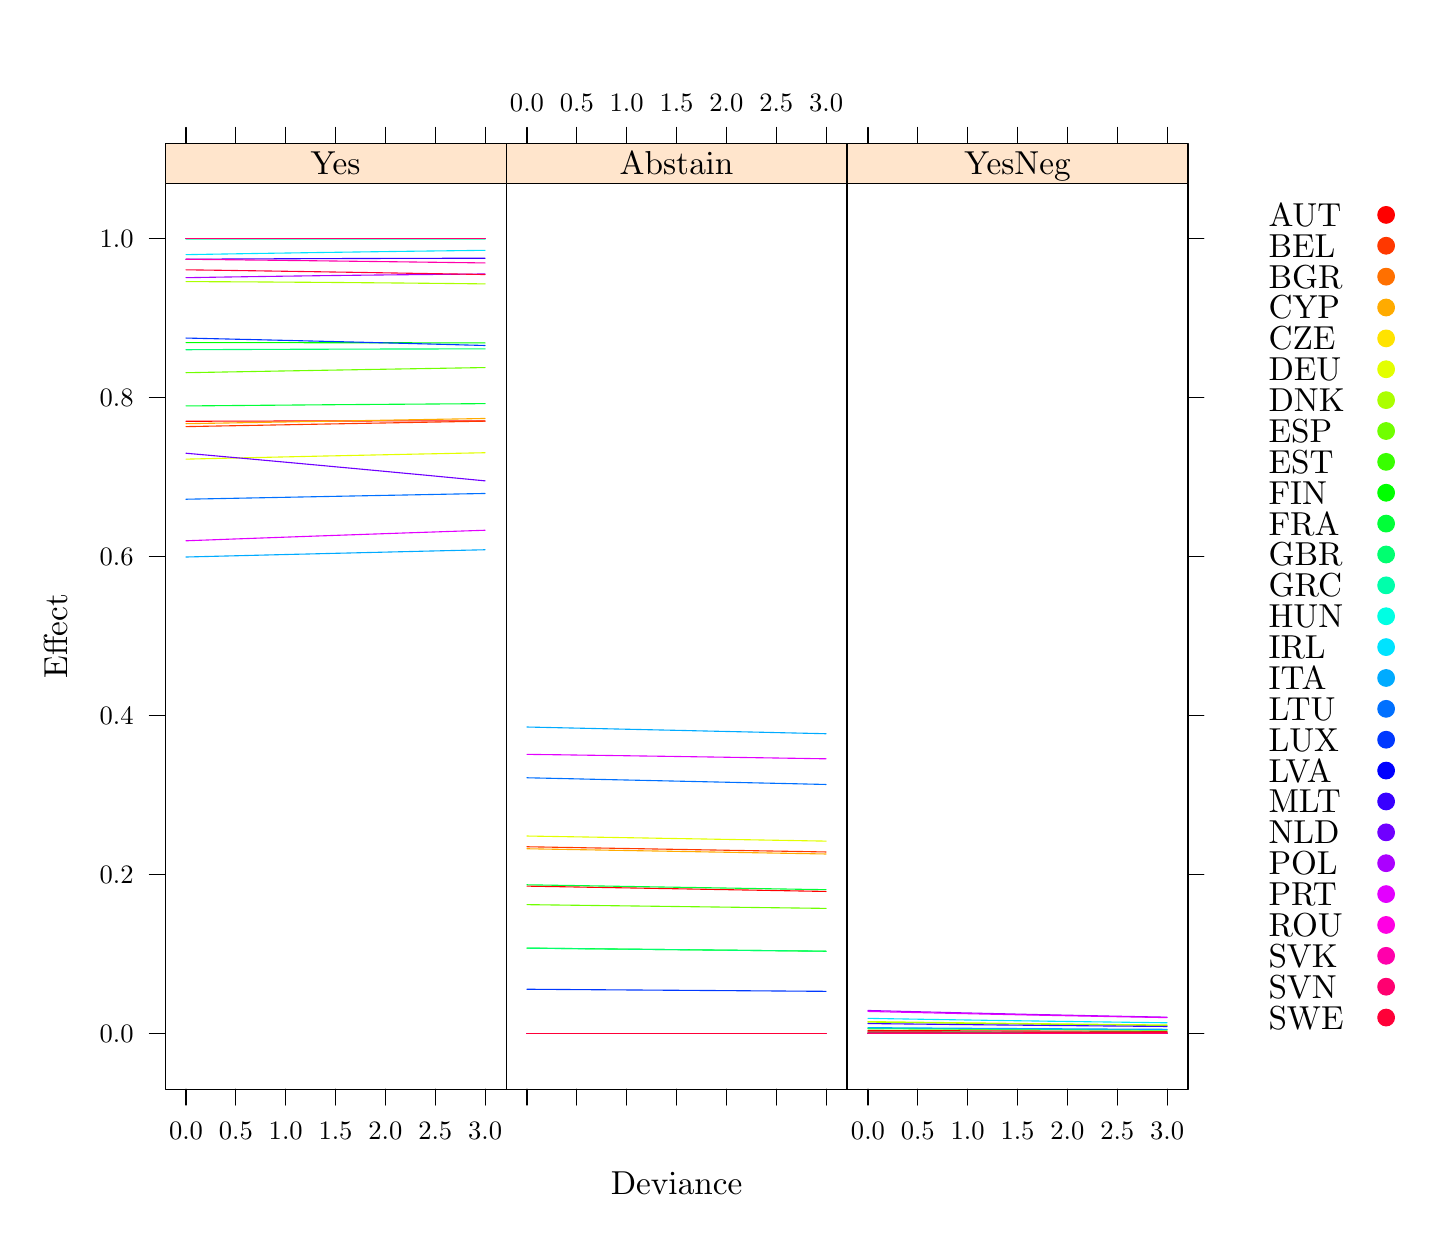
\begin{tikzpicture}[x=1pt,y=1pt]
\definecolor[named]{drawColor}{rgb}{0.00,0.00,0.00}
\definecolor[named]{fillColor}{rgb}{1.00,1.00,1.00}
\fill[color=fillColor,] (0,0) rectangle (505.89,433.62);
\begin{scope}
\path[clip] (  0.00,  0.00) rectangle (505.89,433.62);
\definecolor[named]{fillColor}{rgb}{0.00,0.00,0.00}
\end{scope}
\begin{scope}
\path[clip] (  0.00,  0.00) rectangle (505.89,433.62);
\definecolor[named]{fillColor}{rgb}{0.00,0.00,0.00}

\draw[fill opacity=0.00,draw opacity=0.00,] (  0.00,  0.00) rectangle (505.89,433.62);
\end{scope}
\begin{scope}
\path[clip] (  0.00,  0.00) rectangle (505.89,433.62);
\definecolor[named]{fillColor}{rgb}{0.00,0.00,0.00}
\end{scope}
\begin{scope}
\path[clip] (  0.00,  0.00) rectangle (505.89,433.62);
\definecolor[named]{fillColor}{rgb}{0.00,0.00,0.00}
\definecolor[named]{drawColor}{rgb}{0.00,0.00,0.00}

\node[color=drawColor,anchor=base,inner sep=0pt, outer sep=0pt, scale=  1.20] at (234.47, 12.04) {Deviance%
};
\end{scope}
\begin{scope}
\path[clip] (  0.00,  0.00) rectangle (505.89,433.62);
\definecolor[named]{fillColor}{rgb}{0.00,0.00,0.00}
\definecolor[named]{drawColor}{rgb}{0.00,0.00,0.00}

\node[rotate= 90.00,color=drawColor,anchor=base,inner sep=0pt, outer sep=0pt, scale=  1.20] at ( 14.29,213.72) {Effect%
};
\end{scope}
\begin{scope}
\path[clip] (  0.00,  0.00) rectangle (505.89,433.62);
\definecolor[named]{fillColor}{rgb}{0.00,0.00,0.00}
\end{scope}
\begin{scope}
\path[clip] (  0.00,  0.00) rectangle (505.89,433.62);
\definecolor[named]{fillColor}{rgb}{0.00,0.00,0.00}
\end{scope}
\begin{scope}
\path[clip] (  0.00,  0.00) rectangle (505.89,433.62);
\definecolor[named]{fillColor}{rgb}{0.00,0.00,0.00}
\end{scope}
\begin{scope}
\path[clip] ( 49.65, 50.02) rectangle (172.86,377.42);
\definecolor[named]{fillColor}{rgb}{0.00,0.00,0.00}
\end{scope}
\begin{scope}
\path[clip] (  0.00,  0.00) rectangle (505.89,433.62);
\definecolor[named]{fillColor}{rgb}{0.00,0.00,0.00}
\end{scope}
\begin{scope}
\path[clip] (  0.00,  0.00) rectangle (505.89,433.62);
\definecolor[named]{fillColor}{rgb}{0.00,0.00,0.00}
\definecolor[named]{drawColor}{rgb}{0.00,0.00,0.00}

\draw[color=drawColor,line cap=round,line join=round,fill opacity=0.00,] ( 57.21,391.87) -- ( 57.21,397.56);

\draw[color=drawColor,line cap=round,line join=round,fill opacity=0.00,] ( 75.22,391.87) -- ( 75.22,397.56);

\draw[color=drawColor,line cap=round,line join=round,fill opacity=0.00,] ( 93.24,391.87) -- ( 93.24,397.56);

\draw[color=drawColor,line cap=round,line join=round,fill opacity=0.00,] (111.25,391.87) -- (111.25,397.56);

\draw[color=drawColor,line cap=round,line join=round,fill opacity=0.00,] (129.27,391.87) -- (129.27,397.56);

\draw[color=drawColor,line cap=round,line join=round,fill opacity=0.00,] (147.28,391.87) -- (147.28,397.56);

\draw[color=drawColor,line cap=round,line join=round,fill opacity=0.00,] (165.29,391.87) -- (165.29,397.56);
\end{scope}
\begin{scope}
\path[clip] (  0.00,  0.00) rectangle (505.89,433.62);
\definecolor[named]{fillColor}{rgb}{0.00,0.00,0.00}
\end{scope}
\begin{scope}
\path[clip] (  0.00,  0.00) rectangle (505.89,433.62);
\definecolor[named]{fillColor}{rgb}{0.00,0.00,0.00}
\definecolor[named]{drawColor}{rgb}{0.00,0.00,0.00}

\draw[color=drawColor,line cap=round,line join=round,fill opacity=0.00,] ( 49.65, 70.12) -- ( 43.95, 70.12);

\draw[color=drawColor,line cap=round,line join=round,fill opacity=0.00,] ( 49.65,127.56) -- ( 43.95,127.56);

\draw[color=drawColor,line cap=round,line join=round,fill opacity=0.00,] ( 49.65,185.00) -- ( 43.95,185.00);

\draw[color=drawColor,line cap=round,line join=round,fill opacity=0.00,] ( 49.65,242.43) -- ( 43.95,242.43);

\draw[color=drawColor,line cap=round,line join=round,fill opacity=0.00,] ( 49.65,299.87) -- ( 43.95,299.87);

\draw[color=drawColor,line cap=round,line join=round,fill opacity=0.00,] ( 49.65,357.31) -- ( 43.95,357.31);

\node[color=drawColor,anchor=base east,inner sep=0pt, outer sep=0pt, scale=  0.96] at ( 38.26, 66.81) {0.0%
};

\node[color=drawColor,anchor=base east,inner sep=0pt, outer sep=0pt, scale=  0.96] at ( 38.26,124.25) {0.2%
};

\node[color=drawColor,anchor=base east,inner sep=0pt, outer sep=0pt, scale=  0.96] at ( 38.26,181.69) {0.4%
};

\node[color=drawColor,anchor=base east,inner sep=0pt, outer sep=0pt, scale=  0.96] at ( 38.26,239.13) {0.6%
};

\node[color=drawColor,anchor=base east,inner sep=0pt, outer sep=0pt, scale=  0.96] at ( 38.26,296.57) {0.8%
};

\node[color=drawColor,anchor=base east,inner sep=0pt, outer sep=0pt, scale=  0.96] at ( 38.26,354.01) {1.0%
};
\end{scope}
\begin{scope}
\path[clip] (  0.00,  0.00) rectangle (505.89,433.62);
\definecolor[named]{fillColor}{rgb}{0.00,0.00,0.00}
\end{scope}
\begin{scope}
\path[clip] (  0.00,  0.00) rectangle (505.89,433.62);
\definecolor[named]{fillColor}{rgb}{0.00,0.00,0.00}
\definecolor[named]{drawColor}{rgb}{0.00,0.00,0.00}

\draw[color=drawColor,line cap=round,line join=round,fill opacity=0.00,] ( 57.21, 50.02) -- ( 57.21, 44.32);

\draw[color=drawColor,line cap=round,line join=round,fill opacity=0.00,] ( 75.22, 50.02) -- ( 75.22, 44.32);

\draw[color=drawColor,line cap=round,line join=round,fill opacity=0.00,] ( 93.24, 50.02) -- ( 93.24, 44.32);

\draw[color=drawColor,line cap=round,line join=round,fill opacity=0.00,] (111.25, 50.02) -- (111.25, 44.32);

\draw[color=drawColor,line cap=round,line join=round,fill opacity=0.00,] (129.27, 50.02) -- (129.27, 44.32);

\draw[color=drawColor,line cap=round,line join=round,fill opacity=0.00,] (147.28, 50.02) -- (147.28, 44.32);

\draw[color=drawColor,line cap=round,line join=round,fill opacity=0.00,] (165.29, 50.02) -- (165.29, 44.32);

\node[color=drawColor,anchor=base,inner sep=0pt, outer sep=0pt, scale=  0.96] at ( 57.21, 32.02) {0.0%
};

\node[color=drawColor,anchor=base,inner sep=0pt, outer sep=0pt, scale=  0.96] at ( 75.22, 32.02) {0.5%
};

\node[color=drawColor,anchor=base,inner sep=0pt, outer sep=0pt, scale=  0.96] at ( 93.24, 32.02) {1.0%
};

\node[color=drawColor,anchor=base,inner sep=0pt, outer sep=0pt, scale=  0.96] at (111.25, 32.02) {1.5%
};

\node[color=drawColor,anchor=base,inner sep=0pt, outer sep=0pt, scale=  0.96] at (129.27, 32.02) {2.0%
};

\node[color=drawColor,anchor=base,inner sep=0pt, outer sep=0pt, scale=  0.96] at (147.28, 32.02) {2.5%
};

\node[color=drawColor,anchor=base,inner sep=0pt, outer sep=0pt, scale=  0.96] at (165.29, 32.02) {3.0%
};
\end{scope}
\begin{scope}
\path[clip] (  0.00,  0.00) rectangle (505.89,433.62);
\definecolor[named]{fillColor}{rgb}{0.00,0.00,0.00}
\end{scope}
\begin{scope}
\path[clip] ( 49.65, 50.02) rectangle (172.86,377.42);
\definecolor[named]{fillColor}{rgb}{0.00,0.00,0.00}
\definecolor[named]{drawColor}{rgb}{1.00,0.00,0.00}

\draw[color=drawColor,line cap=round,line join=round,fill opacity=0.00,] ( 57.21,291.39) --
	( 60.81,291.40) --
	( 64.42,291.41) --
	( 68.02,291.42) --
	( 71.62,291.43) --
	( 75.22,291.44) --
	( 78.83,291.45) --
	( 82.43,291.45) --
	( 86.03,291.46) --
	( 89.64,291.47) --
	( 93.24,291.47) --
	( 96.84,291.48) --
	(100.44,291.48) --
	(104.05,291.49) --
	(107.65,291.49) --
	(111.25,291.50) --
	(114.85,291.50) --
	(118.46,291.50) --
	(122.06,291.50) --
	(125.66,291.51) --
	(129.27,291.51) --
	(132.87,291.51) --
	(136.47,291.51) --
	(140.07,291.51) --
	(143.68,291.51) --
	(147.28,291.51) --
	(150.88,291.51) --
	(154.49,291.50) --
	(158.09,291.50) --
	(161.69,291.50) --
	(165.29,291.50);
\definecolor[named]{drawColor}{rgb}{1.00,0.22,0.00}

\draw[color=drawColor,line cap=round,line join=round,fill opacity=0.00,] ( 57.21,289.46) --
	( 60.81,289.52) --
	( 64.42,289.59) --
	( 68.02,289.66) --
	( 71.62,289.73) --
	( 75.22,289.79) --
	( 78.83,289.86) --
	( 82.43,289.92) --
	( 86.03,289.99) --
	( 89.64,290.06) --
	( 93.24,290.12) --
	( 96.84,290.19) --
	(100.44,290.26) --
	(104.05,290.32) --
	(107.65,290.39) --
	(111.25,290.45) --
	(114.85,290.52) --
	(118.46,290.59) --
	(122.06,290.65) --
	(125.66,290.72) --
	(129.27,290.78) --
	(132.87,290.85) --
	(136.47,290.91) --
	(140.07,290.98) --
	(143.68,291.04) --
	(147.28,291.11) --
	(150.88,291.17) --
	(154.49,291.24) --
	(158.09,291.30) --
	(161.69,291.37) --
	(165.29,291.43);
\definecolor[named]{drawColor}{rgb}{1.00,0.44,0.00}

\draw[color=drawColor,line cap=round,line join=round,fill opacity=0.00,] ( 57.21,357.31) --
	( 60.81,357.31) --
	( 64.42,357.31) --
	( 68.02,357.31) --
	( 71.62,357.31) --
	( 75.22,357.31) --
	( 78.83,357.31) --
	( 82.43,357.31) --
	( 86.03,357.31) --
	( 89.64,357.31) --
	( 93.24,357.31) --
	( 96.84,357.31) --
	(100.44,357.31) --
	(104.05,357.31) --
	(107.65,357.31) --
	(111.25,357.31) --
	(114.85,357.31) --
	(118.46,357.31) --
	(122.06,357.31) --
	(125.66,357.31) --
	(129.27,357.31) --
	(132.87,357.31) --
	(136.47,357.31) --
	(140.07,357.31) --
	(143.68,357.31) --
	(147.28,357.31) --
	(150.88,357.31) --
	(154.49,357.31) --
	(158.09,357.31) --
	(161.69,357.31) --
	(165.29,357.31);
\definecolor[named]{drawColor}{rgb}{1.00,0.67,0.00}

\draw[color=drawColor,line cap=round,line join=round,fill opacity=0.00,] ( 57.21,290.51) --
	( 60.81,290.57) --
	( 64.42,290.64) --
	( 68.02,290.70) --
	( 71.62,290.76) --
	( 75.22,290.83) --
	( 78.83,290.89) --
	( 82.43,290.95) --
	( 86.03,291.02) --
	( 89.64,291.08) --
	( 93.24,291.14) --
	( 96.84,291.21) --
	(100.44,291.27) --
	(104.05,291.33) --
	(107.65,291.40) --
	(111.25,291.46) --
	(114.85,291.52) --
	(118.46,291.58) --
	(122.06,291.65) --
	(125.66,291.71) --
	(129.27,291.77) --
	(132.87,291.84) --
	(136.47,291.90) --
	(140.07,291.96) --
	(143.68,292.02) --
	(147.28,292.09) --
	(150.88,292.15) --
	(154.49,292.21) --
	(158.09,292.27) --
	(161.69,292.34) --
	(165.29,292.40);
\definecolor[named]{drawColor}{rgb}{1.00,0.89,0.00}

\draw[color=drawColor,line cap=round,line join=round,fill opacity=0.00,] ( 57.21,357.31) --
	( 60.81,357.31) --
	( 64.42,357.31) --
	( 68.02,357.31) --
	( 71.62,357.31) --
	( 75.22,357.31) --
	( 78.83,357.31) --
	( 82.43,357.31) --
	( 86.03,357.31) --
	( 89.64,357.31) --
	( 93.24,357.31) --
	( 96.84,357.31) --
	(100.44,357.31) --
	(104.05,357.31) --
	(107.65,357.31) --
	(111.25,357.31) --
	(114.85,357.31) --
	(118.46,357.31) --
	(122.06,357.31) --
	(125.66,357.31) --
	(129.27,357.31) --
	(132.87,357.31) --
	(136.47,357.31) --
	(140.07,357.31) --
	(143.68,357.31) --
	(147.28,357.31) --
	(150.88,357.31) --
	(154.49,357.31) --
	(158.09,357.31) --
	(161.69,357.31) --
	(165.29,357.31);
\definecolor[named]{drawColor}{rgb}{0.89,1.00,0.00}

\draw[color=drawColor,line cap=round,line join=round,fill opacity=0.00,] ( 57.21,277.70) --
	( 60.81,277.79) --
	( 64.42,277.87) --
	( 68.02,277.95) --
	( 71.62,278.04) --
	( 75.22,278.12) --
	( 78.83,278.20) --
	( 82.43,278.28) --
	( 86.03,278.36) --
	( 89.64,278.44) --
	( 93.24,278.52) --
	( 96.84,278.60) --
	(100.44,278.68) --
	(104.05,278.76) --
	(107.65,278.84) --
	(111.25,278.91) --
	(114.85,278.99) --
	(118.46,279.07) --
	(122.06,279.14) --
	(125.66,279.22) --
	(129.27,279.29) --
	(132.87,279.37) --
	(136.47,279.44) --
	(140.07,279.52) --
	(143.68,279.59) --
	(147.28,279.66) --
	(150.88,279.73) --
	(154.49,279.81) --
	(158.09,279.88) --
	(161.69,279.95) --
	(165.29,280.02);
\definecolor[named]{drawColor}{rgb}{0.67,1.00,0.00}

\draw[color=drawColor,line cap=round,line join=round,fill opacity=0.00,] ( 57.21,341.86) --
	( 60.81,341.85) --
	( 64.42,341.83) --
	( 68.02,341.81) --
	( 71.62,341.79) --
	( 75.22,341.78) --
	( 78.83,341.76) --
	( 82.43,341.74) --
	( 86.03,341.71) --
	( 89.64,341.69) --
	( 93.24,341.67) --
	( 96.84,341.64) --
	(100.44,341.62) --
	(104.05,341.59) --
	(107.65,341.57) --
	(111.25,341.54) --
	(114.85,341.51) --
	(118.46,341.48) --
	(122.06,341.45) --
	(125.66,341.42) --
	(129.27,341.39) --
	(132.87,341.36) --
	(136.47,341.33) --
	(140.07,341.29) --
	(143.68,341.26) --
	(147.28,341.22) --
	(150.88,341.19) --
	(154.49,341.15) --
	(158.09,341.11) --
	(161.69,341.07) --
	(165.29,341.03);
\definecolor[named]{drawColor}{rgb}{0.44,1.00,0.00}

\draw[color=drawColor,line cap=round,line join=round,fill opacity=0.00,] ( 57.21,308.94) --
	( 60.81,309.00) --
	( 64.42,309.07) --
	( 68.02,309.13) --
	( 71.62,309.20) --
	( 75.22,309.26) --
	( 78.83,309.32) --
	( 82.43,309.39) --
	( 86.03,309.45) --
	( 89.64,309.52) --
	( 93.24,309.58) --
	( 96.84,309.64) --
	(100.44,309.70) --
	(104.05,309.77) --
	(107.65,309.83) --
	(111.25,309.89) --
	(114.85,309.95) --
	(118.46,310.01) --
	(122.06,310.08) --
	(125.66,310.14) --
	(129.27,310.20) --
	(132.87,310.26) --
	(136.47,310.32) --
	(140.07,310.38) --
	(143.68,310.44) --
	(147.28,310.50) --
	(150.88,310.56) --
	(154.49,310.62) --
	(158.09,310.68) --
	(161.69,310.74) --
	(165.29,310.80);
\definecolor[named]{drawColor}{rgb}{0.22,1.00,0.00}

\draw[color=drawColor,line cap=round,line join=round,fill opacity=0.00,] ( 57.21,357.31) --
	( 60.81,357.31) --
	( 64.42,357.31) --
	( 68.02,357.31) --
	( 71.62,357.31) --
	( 75.22,357.31) --
	( 78.83,357.31) --
	( 82.43,357.31) --
	( 86.03,357.31) --
	( 89.64,357.31) --
	( 93.24,357.31) --
	( 96.84,357.31) --
	(100.44,357.31) --
	(104.05,357.31) --
	(107.65,357.31) --
	(111.25,357.31) --
	(114.85,357.31) --
	(118.46,357.31) --
	(122.06,357.31) --
	(125.66,357.31) --
	(129.27,357.31) --
	(132.87,357.31) --
	(136.47,357.31) --
	(140.07,357.31) --
	(143.68,357.31) --
	(147.28,357.31) --
	(150.88,357.31) --
	(154.49,357.31) --
	(158.09,357.31) --
	(161.69,357.31) --
	(165.29,357.31);
\definecolor[named]{drawColor}{rgb}{0.00,1.00,0.00}

\draw[color=drawColor,line cap=round,line join=round,fill opacity=0.00,] ( 57.21,319.79) --
	( 60.81,319.79) --
	( 64.42,319.79) --
	( 68.02,319.79) --
	( 71.62,319.79) --
	( 75.22,319.79) --
	( 78.83,319.79) --
	( 82.43,319.79) --
	( 86.03,319.79) --
	( 89.64,319.79) --
	( 93.24,319.79) --
	( 96.84,319.79) --
	(100.44,319.78) --
	(104.05,319.78) --
	(107.65,319.78) --
	(111.25,319.78) --
	(114.85,319.77) --
	(118.46,319.77) --
	(122.06,319.77) --
	(125.66,319.76) --
	(129.27,319.76) --
	(132.87,319.75) --
	(136.47,319.75) --
	(140.07,319.74) --
	(143.68,319.74) --
	(147.28,319.73) --
	(150.88,319.73) --
	(154.49,319.72) --
	(158.09,319.72) --
	(161.69,319.71) --
	(165.29,319.70);
\definecolor[named]{drawColor}{rgb}{0.00,1.00,0.22}

\draw[color=drawColor,line cap=round,line join=round,fill opacity=0.00,] ( 57.21,296.93) --
	( 60.81,296.96) --
	( 64.42,296.99) --
	( 68.02,297.02) --
	( 71.62,297.05) --
	( 75.22,297.08) --
	( 78.83,297.11) --
	( 82.43,297.15) --
	( 86.03,297.17) --
	( 89.64,297.20) --
	( 93.24,297.23) --
	( 96.84,297.26) --
	(100.44,297.29) --
	(104.05,297.32) --
	(107.65,297.35) --
	(111.25,297.38) --
	(114.85,297.40) --
	(118.46,297.43) --
	(122.06,297.46) --
	(125.66,297.48) --
	(129.27,297.51) --
	(132.87,297.54) --
	(136.47,297.56) --
	(140.07,297.59) --
	(143.68,297.61) --
	(147.28,297.64) --
	(150.88,297.66) --
	(154.49,297.69) --
	(158.09,297.71) --
	(161.69,297.74) --
	(165.29,297.76);
\definecolor[named]{drawColor}{rgb}{0.00,1.00,0.44}

\draw[color=drawColor,line cap=round,line join=round,fill opacity=0.00,] ( 57.21,317.24) --
	( 60.81,317.26) --
	( 64.42,317.27) --
	( 68.02,317.29) --
	( 71.62,317.31) --
	( 75.22,317.32) --
	( 78.83,317.33) --
	( 82.43,317.35) --
	( 86.03,317.36) --
	( 89.64,317.37) --
	( 93.24,317.39) --
	( 96.84,317.40) --
	(100.44,317.41) --
	(104.05,317.42) --
	(107.65,317.43) --
	(111.25,317.44) --
	(114.85,317.45) --
	(118.46,317.46) --
	(122.06,317.47) --
	(125.66,317.48) --
	(129.27,317.49) --
	(132.87,317.49) --
	(136.47,317.50) --
	(140.07,317.51) --
	(143.68,317.51) --
	(147.28,317.52) --
	(150.88,317.53) --
	(154.49,317.53) --
	(158.09,317.53) --
	(161.69,317.54) --
	(165.29,317.54);
\definecolor[named]{drawColor}{rgb}{0.00,1.00,0.67}

\draw[color=drawColor,line cap=round,line join=round,fill opacity=0.00,] ( 57.21,357.23) --
	( 60.81,357.23) --
	( 64.42,357.23) --
	( 68.02,357.23) --
	( 71.62,357.23) --
	( 75.22,357.22) --
	( 78.83,357.22) --
	( 82.43,357.22) --
	( 86.03,357.22) --
	( 89.64,357.22) --
	( 93.24,357.22) --
	( 96.84,357.22) --
	(100.44,357.22) --
	(104.05,357.22) --
	(107.65,357.22) --
	(111.25,357.22) --
	(114.85,357.22) --
	(118.46,357.22) --
	(122.06,357.22) --
	(125.66,357.22) --
	(129.27,357.22) --
	(132.87,357.22) --
	(136.47,357.22) --
	(140.07,357.22) --
	(143.68,357.22) --
	(147.28,357.21) --
	(150.88,357.21) --
	(154.49,357.21) --
	(158.09,357.21) --
	(161.69,357.21) --
	(165.29,357.21);
\definecolor[named]{drawColor}{rgb}{0.00,1.00,0.89}

\draw[color=drawColor,line cap=round,line join=round,fill opacity=0.00,] ( 57.21,357.31) --
	( 60.81,357.31) --
	( 64.42,357.31) --
	( 68.02,357.31) --
	( 71.62,357.31) --
	( 75.22,357.31) --
	( 78.83,357.31) --
	( 82.43,357.31) --
	( 86.03,357.31) --
	( 89.64,357.31) --
	( 93.24,357.31) --
	( 96.84,357.31) --
	(100.44,357.31) --
	(104.05,357.31) --
	(107.65,357.31) --
	(111.25,357.31) --
	(114.85,357.31) --
	(118.46,357.31) --
	(122.06,357.31) --
	(125.66,357.31) --
	(129.27,357.31) --
	(132.87,357.31) --
	(136.47,357.31) --
	(140.07,357.31) --
	(143.68,357.31) --
	(147.28,357.31) --
	(150.88,357.31) --
	(154.49,357.31) --
	(158.09,357.31) --
	(161.69,357.31) --
	(165.29,357.31);
\definecolor[named]{drawColor}{rgb}{0.00,0.89,1.00}

\draw[color=drawColor,line cap=round,line join=round,fill opacity=0.00,] ( 57.21,351.60) --
	( 60.81,351.66) --
	( 64.42,351.72) --
	( 68.02,351.78) --
	( 71.62,351.84) --
	( 75.22,351.90) --
	( 78.83,351.96) --
	( 82.43,352.02) --
	( 86.03,352.07) --
	( 89.64,352.13) --
	( 93.24,352.18) --
	( 96.84,352.24) --
	(100.44,352.29) --
	(104.05,352.35) --
	(107.65,352.40) --
	(111.25,352.45) --
	(114.85,352.50) --
	(118.46,352.55) --
	(122.06,352.60) --
	(125.66,352.65) --
	(129.27,352.70) --
	(132.87,352.75) --
	(136.47,352.80) --
	(140.07,352.85) --
	(143.68,352.89) --
	(147.28,352.94) --
	(150.88,352.98) --
	(154.49,353.03) --
	(158.09,353.07) --
	(161.69,353.12) --
	(165.29,353.16);
\definecolor[named]{drawColor}{rgb}{0.00,0.67,1.00}

\draw[color=drawColor,line cap=round,line join=round,fill opacity=0.00,] ( 57.21,242.34) --
	( 60.81,242.43) --
	( 64.42,242.52) --
	( 68.02,242.61) --
	( 71.62,242.70) --
	( 75.22,242.79) --
	( 78.83,242.88) --
	( 82.43,242.97) --
	( 86.03,243.06) --
	( 89.64,243.15) --
	( 93.24,243.24) --
	( 96.84,243.33) --
	(100.44,243.41) --
	(104.05,243.50) --
	(107.65,243.59) --
	(111.25,243.68) --
	(114.85,243.76) --
	(118.46,243.85) --
	(122.06,243.94) --
	(125.66,244.02) --
	(129.27,244.11) --
	(132.87,244.20) --
	(136.47,244.28) --
	(140.07,244.37) --
	(143.68,244.46) --
	(147.28,244.54) --
	(150.88,244.63) --
	(154.49,244.71) --
	(158.09,244.80) --
	(161.69,244.88) --
	(165.29,244.96);
\definecolor[named]{drawColor}{rgb}{0.00,0.44,1.00}

\draw[color=drawColor,line cap=round,line join=round,fill opacity=0.00,] ( 57.21,263.22) --
	( 60.81,263.29) --
	( 64.42,263.36) --
	( 68.02,263.43) --
	( 71.62,263.50) --
	( 75.22,263.57) --
	( 78.83,263.64) --
	( 82.43,263.71) --
	( 86.03,263.78) --
	( 89.64,263.85) --
	( 93.24,263.92) --
	( 96.84,263.99) --
	(100.44,264.06) --
	(104.05,264.13) --
	(107.65,264.20) --
	(111.25,264.27) --
	(114.85,264.34) --
	(118.46,264.41) --
	(122.06,264.48) --
	(125.66,264.55) --
	(129.27,264.62) --
	(132.87,264.68) --
	(136.47,264.75) --
	(140.07,264.82) --
	(143.68,264.89) --
	(147.28,264.96) --
	(150.88,265.03) --
	(154.49,265.10) --
	(158.09,265.17) --
	(161.69,265.23) --
	(165.29,265.30);
\definecolor[named]{drawColor}{rgb}{0.00,0.22,1.00}

\draw[color=drawColor,line cap=round,line join=round,fill opacity=0.00,] ( 57.21,321.46) --
	( 60.81,321.38) --
	( 64.42,321.29) --
	( 68.02,321.21) --
	( 71.62,321.13) --
	( 75.22,321.04) --
	( 78.83,320.96) --
	( 82.43,320.88) --
	( 86.03,320.79) --
	( 89.64,320.70) --
	( 93.24,320.62) --
	( 96.84,320.53) --
	(100.44,320.44) --
	(104.05,320.35) --
	(107.65,320.27) --
	(111.25,320.18) --
	(114.85,320.09) --
	(118.46,320.00) --
	(122.06,319.91) --
	(125.66,319.81) --
	(129.27,319.72) --
	(132.87,319.63) --
	(136.47,319.54) --
	(140.07,319.44) --
	(143.68,319.35) --
	(147.28,319.25) --
	(150.88,319.16) --
	(154.49,319.06) --
	(158.09,318.96) --
	(161.69,318.87) --
	(165.29,318.77);
\definecolor[named]{drawColor}{rgb}{0.00,0.00,1.00}

\draw[color=drawColor,line cap=round,line join=round,fill opacity=0.00,] ( 57.21,357.31) --
	( 60.81,357.31) --
	( 64.42,357.31) --
	( 68.02,357.31) --
	( 71.62,357.31) --
	( 75.22,357.31) --
	( 78.83,357.31) --
	( 82.43,357.31) --
	( 86.03,357.31) --
	( 89.64,357.31) --
	( 93.24,357.31) --
	( 96.84,357.31) --
	(100.44,357.31) --
	(104.05,357.31) --
	(107.65,357.31) --
	(111.25,357.31) --
	(114.85,357.31) --
	(118.46,357.31) --
	(122.06,357.31) --
	(125.66,357.31) --
	(129.27,357.31) --
	(132.87,357.31) --
	(136.47,357.31) --
	(140.07,357.31) --
	(143.68,357.31) --
	(147.28,357.31) --
	(150.88,357.31) --
	(154.49,357.31) --
	(158.09,357.31) --
	(161.69,357.31) --
	(165.29,357.31);
\definecolor[named]{drawColor}{rgb}{0.22,0.00,1.00}

\draw[color=drawColor,line cap=round,line join=round,fill opacity=0.00,] ( 57.21,349.94) --
	( 60.81,349.96) --
	( 64.42,349.98) --
	( 68.02,350.00) --
	( 71.62,350.01) --
	( 75.22,350.03) --
	( 78.83,350.05) --
	( 82.43,350.07) --
	( 86.03,350.08) --
	( 89.64,350.10) --
	( 93.24,350.11) --
	( 96.84,350.13) --
	(100.44,350.14) --
	(104.05,350.15) --
	(107.65,350.17) --
	(111.25,350.18) --
	(114.85,350.19) --
	(118.46,350.20) --
	(122.06,350.21) --
	(125.66,350.22) --
	(129.27,350.23) --
	(132.87,350.24) --
	(136.47,350.25) --
	(140.07,350.26) --
	(143.68,350.27) --
	(147.28,350.27) --
	(150.88,350.28) --
	(154.49,350.29) --
	(158.09,350.29) --
	(161.69,350.30) --
	(165.29,350.30);
\definecolor[named]{drawColor}{rgb}{0.44,0.00,1.00}

\draw[color=drawColor,line cap=round,line join=round,fill opacity=0.00,] ( 57.21,279.84) --
	( 60.81,279.52) --
	( 64.42,279.20) --
	( 68.02,278.88) --
	( 71.62,278.55) --
	( 75.22,278.23) --
	( 78.83,277.91) --
	( 82.43,277.58) --
	( 86.03,277.25) --
	( 89.64,276.93) --
	( 93.24,276.60) --
	( 96.84,276.27) --
	(100.44,275.94) --
	(104.05,275.61) --
	(107.65,275.28) --
	(111.25,274.94) --
	(114.85,274.61) --
	(118.46,274.28) --
	(122.06,273.94) --
	(125.66,273.61) --
	(129.27,273.27) --
	(132.87,272.93) --
	(136.47,272.59) --
	(140.07,272.26) --
	(143.68,271.92) --
	(147.28,271.58) --
	(150.88,271.23) --
	(154.49,270.89) --
	(158.09,270.55) --
	(161.69,270.20) --
	(165.29,269.86);
\definecolor[named]{drawColor}{rgb}{0.67,0.00,1.00}

\draw[color=drawColor,line cap=round,line join=round,fill opacity=0.00,] ( 57.21,343.27) --
	( 60.81,343.33) --
	( 64.42,343.39) --
	( 68.02,343.45) --
	( 71.62,343.51) --
	( 75.22,343.56) --
	( 78.83,343.62) --
	( 82.43,343.67) --
	( 86.03,343.72) --
	( 89.64,343.77) --
	( 93.24,343.83) --
	( 96.84,343.87) --
	(100.44,343.92) --
	(104.05,343.97) --
	(107.65,344.02) --
	(111.25,344.06) --
	(114.85,344.10) --
	(118.46,344.15) --
	(122.06,344.19) --
	(125.66,344.23) --
	(129.27,344.27) --
	(132.87,344.31) --
	(136.47,344.34) --
	(140.07,344.38) --
	(143.68,344.42) --
	(147.28,344.45) --
	(150.88,344.48) --
	(154.49,344.52) --
	(158.09,344.55) --
	(161.69,344.58) --
	(165.29,344.61);
\definecolor[named]{drawColor}{rgb}{0.89,0.00,1.00}

\draw[color=drawColor,line cap=round,line join=round,fill opacity=0.00,] ( 57.21,248.20) --
	( 60.81,248.34) --
	( 64.42,248.47) --
	( 68.02,248.60) --
	( 71.62,248.74) --
	( 75.22,248.87) --
	( 78.83,249.00) --
	( 82.43,249.13) --
	( 86.03,249.26) --
	( 89.64,249.39) --
	( 93.24,249.52) --
	( 96.84,249.65) --
	(100.44,249.78) --
	(104.05,249.91) --
	(107.65,250.03) --
	(111.25,250.16) --
	(114.85,250.29) --
	(118.46,250.41) --
	(122.06,250.54) --
	(125.66,250.66) --
	(129.27,250.79) --
	(132.87,250.91) --
	(136.47,251.04) --
	(140.07,251.16) --
	(143.68,251.28) --
	(147.28,251.40) --
	(150.88,251.53) --
	(154.49,251.65) --
	(158.09,251.77) --
	(161.69,251.89) --
	(165.29,252.01);
\definecolor[named]{drawColor}{rgb}{1.00,0.00,0.89}

\draw[color=drawColor,line cap=round,line join=round,fill opacity=0.00,] ( 57.21,357.31) --
	( 60.81,357.31) --
	( 64.42,357.31) --
	( 68.02,357.31) --
	( 71.62,357.31) --
	( 75.22,357.31) --
	( 78.83,357.31) --
	( 82.43,357.31) --
	( 86.03,357.31) --
	( 89.64,357.31) --
	( 93.24,357.31) --
	( 96.84,357.31) --
	(100.44,357.31) --
	(104.05,357.31) --
	(107.65,357.31) --
	(111.25,357.31) --
	(114.85,357.31) --
	(118.46,357.31) --
	(122.06,357.31) --
	(125.66,357.31) --
	(129.27,357.31) --
	(132.87,357.31) --
	(136.47,357.31) --
	(140.07,357.31) --
	(143.68,357.31) --
	(147.28,357.31) --
	(150.88,357.31) --
	(154.49,357.31) --
	(158.09,357.31) --
	(161.69,357.31) --
	(165.29,357.31);
\definecolor[named]{drawColor}{rgb}{1.00,0.00,0.67}

\draw[color=drawColor,line cap=round,line join=round,fill opacity=0.00,] ( 57.21,349.93) --
	( 60.81,349.89) --
	( 64.42,349.85) --
	( 68.02,349.81) --
	( 71.62,349.77) --
	( 75.22,349.73) --
	( 78.83,349.68) --
	( 82.43,349.64) --
	( 86.03,349.60) --
	( 89.64,349.56) --
	( 93.24,349.51) --
	( 96.84,349.47) --
	(100.44,349.43) --
	(104.05,349.38) --
	(107.65,349.34) --
	(111.25,349.29) --
	(114.85,349.25) --
	(118.46,349.20) --
	(122.06,349.16) --
	(125.66,349.11) --
	(129.27,349.07) --
	(132.87,349.02) --
	(136.47,348.98) --
	(140.07,348.93) --
	(143.68,348.88) --
	(147.28,348.84) --
	(150.88,348.79) --
	(154.49,348.74) --
	(158.09,348.70) --
	(161.69,348.65) --
	(165.29,348.60);
\definecolor[named]{drawColor}{rgb}{1.00,0.00,0.44}

\draw[color=drawColor,line cap=round,line join=round,fill opacity=0.00,] ( 57.21,357.31) --
	( 60.81,357.31) --
	( 64.42,357.31) --
	( 68.02,357.31) --
	( 71.62,357.31) --
	( 75.22,357.31) --
	( 78.83,357.31) --
	( 82.43,357.31) --
	( 86.03,357.31) --
	( 89.64,357.31) --
	( 93.24,357.31) --
	( 96.84,357.31) --
	(100.44,357.31) --
	(104.05,357.31) --
	(107.65,357.31) --
	(111.25,357.31) --
	(114.85,357.31) --
	(118.46,357.31) --
	(122.06,357.31) --
	(125.66,357.31) --
	(129.27,357.31) --
	(132.87,357.31) --
	(136.47,357.31) --
	(140.07,357.31) --
	(143.68,357.31) --
	(147.28,357.31) --
	(150.88,357.31) --
	(154.49,357.31) --
	(158.09,357.31) --
	(161.69,357.31) --
	(165.29,357.31);
\definecolor[named]{drawColor}{rgb}{1.00,0.00,0.22}

\draw[color=drawColor,line cap=round,line join=round,fill opacity=0.00,] ( 57.21,346.12) --
	( 60.81,346.07) --
	( 64.42,346.02) --
	( 68.02,345.97) --
	( 71.62,345.92) --
	( 75.22,345.86) --
	( 78.83,345.81) --
	( 82.43,345.76) --
	( 86.03,345.70) --
	( 89.64,345.65) --
	( 93.24,345.59) --
	( 96.84,345.54) --
	(100.44,345.48) --
	(104.05,345.43) --
	(107.65,345.37) --
	(111.25,345.31) --
	(114.85,345.26) --
	(118.46,345.20) --
	(122.06,345.14) --
	(125.66,345.08) --
	(129.27,345.02) --
	(132.87,344.96) --
	(136.47,344.90) --
	(140.07,344.84) --
	(143.68,344.78) --
	(147.28,344.72) --
	(150.88,344.66) --
	(154.49,344.60) --
	(158.09,344.54) --
	(161.69,344.48) --
	(165.29,344.41);
\end{scope}
\begin{scope}
\path[clip] (  0.00,  0.00) rectangle (505.89,433.62);
\definecolor[named]{fillColor}{rgb}{0.00,0.00,0.00}
\end{scope}
\begin{scope}
\path[clip] (  0.00,  0.00) rectangle (505.89,433.62);
\definecolor[named]{fillColor}{rgb}{0.00,0.00,0.00}
\definecolor[named]{drawColor}{rgb}{0.00,0.00,0.00}

\draw[color=drawColor,line cap=round,line join=round,fill opacity=0.00,] ( 49.65, 50.02) rectangle (172.86,377.42);
\end{scope}
\begin{scope}
\path[clip] (  0.00,  0.00) rectangle (505.89,433.62);
\definecolor[named]{fillColor}{rgb}{0.00,0.00,0.00}
\end{scope}
\begin{scope}
\path[clip] (  0.00,  0.00) rectangle (505.89,433.62);
\definecolor[named]{fillColor}{rgb}{0.00,0.00,0.00}
\end{scope}
\begin{scope}
\path[clip] ( 49.65,377.42) rectangle (172.86,391.87);
\definecolor[named]{fillColor}{rgb}{0.00,0.00,0.00}
\definecolor[named]{drawColor}{rgb}{1.00,0.90,0.80}
\definecolor[named]{fillColor}{rgb}{1.00,0.90,0.80}

\draw[color=drawColor,line cap=round,line join=round,fill=fillColor,] ( 49.65,377.42) rectangle (172.86,391.87);
\definecolor[named]{drawColor}{rgb}{0.00,0.00,0.00}

\node[color=drawColor,anchor=base west,inner sep=0pt, outer sep=0pt, scale=  1.20] at (102.22,380.51) {Yes%
};
\end{scope}
\begin{scope}
\path[clip] (  0.00,  0.00) rectangle (505.89,433.62);
\definecolor[named]{fillColor}{rgb}{0.00,0.00,0.00}
\end{scope}
\begin{scope}
\path[clip] (  0.00,  0.00) rectangle (505.89,433.62);
\definecolor[named]{fillColor}{rgb}{0.00,0.00,0.00}
\definecolor[named]{drawColor}{rgb}{0.00,0.00,0.00}

\draw[color=drawColor,line cap=round,line join=round,fill opacity=0.00,] ( 49.65,377.42) rectangle (172.86,391.87);
\end{scope}
\begin{scope}
\path[clip] (  0.00,  0.00) rectangle (505.89,433.62);
\definecolor[named]{fillColor}{rgb}{0.00,0.00,0.00}
\end{scope}
\begin{scope}
\path[clip] (  0.00,  0.00) rectangle (505.89,433.62);
\definecolor[named]{fillColor}{rgb}{0.00,0.00,0.00}
\end{scope}
\begin{scope}
\path[clip] (172.86, 50.02) rectangle (296.07,377.42);
\definecolor[named]{fillColor}{rgb}{0.00,0.00,0.00}
\end{scope}
\begin{scope}
\path[clip] (  0.00,  0.00) rectangle (505.89,433.62);
\definecolor[named]{fillColor}{rgb}{0.00,0.00,0.00}
\end{scope}
\begin{scope}
\path[clip] (  0.00,  0.00) rectangle (505.89,433.62);
\definecolor[named]{fillColor}{rgb}{0.00,0.00,0.00}
\definecolor[named]{drawColor}{rgb}{0.00,0.00,0.00}

\draw[color=drawColor,line cap=round,line join=round,fill opacity=0.00,] (180.42,391.87) -- (180.42,397.56);

\draw[color=drawColor,line cap=round,line join=round,fill opacity=0.00,] (198.44,391.87) -- (198.44,397.56);

\draw[color=drawColor,line cap=round,line join=round,fill opacity=0.00,] (216.45,391.87) -- (216.45,397.56);

\draw[color=drawColor,line cap=round,line join=round,fill opacity=0.00,] (234.47,391.87) -- (234.47,397.56);

\draw[color=drawColor,line cap=round,line join=round,fill opacity=0.00,] (252.48,391.87) -- (252.48,397.56);

\draw[color=drawColor,line cap=round,line join=round,fill opacity=0.00,] (270.49,391.87) -- (270.49,397.56);

\draw[color=drawColor,line cap=round,line join=round,fill opacity=0.00,] (288.51,391.87) -- (288.51,397.56);

\node[color=drawColor,anchor=base,inner sep=0pt, outer sep=0pt, scale=  0.96] at (180.42,403.25) {0.0%
};

\node[color=drawColor,anchor=base,inner sep=0pt, outer sep=0pt, scale=  0.96] at (198.44,403.25) {0.5%
};

\node[color=drawColor,anchor=base,inner sep=0pt, outer sep=0pt, scale=  0.96] at (216.45,403.25) {1.0%
};

\node[color=drawColor,anchor=base,inner sep=0pt, outer sep=0pt, scale=  0.96] at (234.47,403.25) {1.5%
};

\node[color=drawColor,anchor=base,inner sep=0pt, outer sep=0pt, scale=  0.96] at (252.48,403.25) {2.0%
};

\node[color=drawColor,anchor=base,inner sep=0pt, outer sep=0pt, scale=  0.96] at (270.49,403.25) {2.5%
};

\node[color=drawColor,anchor=base,inner sep=0pt, outer sep=0pt, scale=  0.96] at (288.51,403.25) {3.0%
};
\end{scope}
\begin{scope}
\path[clip] (  0.00,  0.00) rectangle (505.89,433.62);
\definecolor[named]{fillColor}{rgb}{0.00,0.00,0.00}
\end{scope}
\begin{scope}
\path[clip] (  0.00,  0.00) rectangle (505.89,433.62);
\definecolor[named]{fillColor}{rgb}{0.00,0.00,0.00}
\end{scope}
\begin{scope}
\path[clip] (  0.00,  0.00) rectangle (505.89,433.62);
\definecolor[named]{fillColor}{rgb}{0.00,0.00,0.00}
\end{scope}
\begin{scope}
\path[clip] (  0.00,  0.00) rectangle (505.89,433.62);
\definecolor[named]{fillColor}{rgb}{0.00,0.00,0.00}
\definecolor[named]{drawColor}{rgb}{0.00,0.00,0.00}

\draw[color=drawColor,line cap=round,line join=round,fill opacity=0.00,] (180.42, 50.02) -- (180.42, 44.32);

\draw[color=drawColor,line cap=round,line join=round,fill opacity=0.00,] (198.44, 50.02) -- (198.44, 44.32);

\draw[color=drawColor,line cap=round,line join=round,fill opacity=0.00,] (216.45, 50.02) -- (216.45, 44.32);

\draw[color=drawColor,line cap=round,line join=round,fill opacity=0.00,] (234.47, 50.02) -- (234.47, 44.32);

\draw[color=drawColor,line cap=round,line join=round,fill opacity=0.00,] (252.48, 50.02) -- (252.48, 44.32);

\draw[color=drawColor,line cap=round,line join=round,fill opacity=0.00,] (270.49, 50.02) -- (270.49, 44.32);

\draw[color=drawColor,line cap=round,line join=round,fill opacity=0.00,] (288.51, 50.02) -- (288.51, 44.32);
\end{scope}
\begin{scope}
\path[clip] (  0.00,  0.00) rectangle (505.89,433.62);
\definecolor[named]{fillColor}{rgb}{0.00,0.00,0.00}
\end{scope}
\begin{scope}
\path[clip] (172.86, 50.02) rectangle (296.07,377.42);
\definecolor[named]{fillColor}{rgb}{0.00,0.00,0.00}
\definecolor[named]{drawColor}{rgb}{1.00,0.00,0.00}

\draw[color=drawColor,line cap=round,line join=round,fill opacity=0.00,] (180.42,123.42) --
	(184.03,123.35) --
	(187.63,123.29) --
	(191.23,123.23) --
	(194.84,123.16) --
	(198.44,123.10) --
	(202.04,123.03) --
	(205.64,122.97) --
	(209.25,122.91) --
	(212.85,122.84) --
	(216.45,122.78) --
	(220.06,122.72) --
	(223.66,122.65) --
	(227.26,122.59) --
	(230.86,122.52) --
	(234.47,122.46) --
	(238.07,122.40) --
	(241.67,122.33) --
	(245.27,122.27) --
	(248.88,122.20) --
	(252.48,122.14) --
	(256.08,122.07) --
	(259.69,122.01) --
	(263.29,121.95) --
	(266.89,121.88) --
	(270.49,121.82) --
	(274.10,121.75) --
	(277.70,121.69) --
	(281.30,121.62) --
	(284.90,121.56) --
	(288.51,121.49);
\definecolor[named]{drawColor}{rgb}{1.00,0.22,0.00}

\draw[color=drawColor,line cap=round,line join=round,fill opacity=0.00,] (180.42,137.64) --
	(184.03,137.58) --
	(187.63,137.52) --
	(191.23,137.45) --
	(194.84,137.39) --
	(198.44,137.33) --
	(202.04,137.26) --
	(205.64,137.20) --
	(209.25,137.14) --
	(212.85,137.07) --
	(216.45,137.01) --
	(220.06,136.95) --
	(223.66,136.89) --
	(227.26,136.82) --
	(230.86,136.76) --
	(234.47,136.70) --
	(238.07,136.64) --
	(241.67,136.57) --
	(245.27,136.51) --
	(248.88,136.45) --
	(252.48,136.38) --
	(256.08,136.32) --
	(259.69,136.26) --
	(263.29,136.20) --
	(266.89,136.13) --
	(270.49,136.07) --
	(274.10,136.01) --
	(277.70,135.95) --
	(281.30,135.89) --
	(284.90,135.82) --
	(288.51,135.76);
\definecolor[named]{drawColor}{rgb}{1.00,0.44,0.00}

\draw[color=drawColor,line cap=round,line join=round,fill opacity=0.00,] (180.42, 70.12) --
	(184.03, 70.12) --
	(187.63, 70.12) --
	(191.23, 70.12) --
	(194.84, 70.12) --
	(198.44, 70.12) --
	(202.04, 70.12) --
	(205.64, 70.12) --
	(209.25, 70.12) --
	(212.85, 70.12) --
	(216.45, 70.12) --
	(220.06, 70.12) --
	(223.66, 70.12) --
	(227.26, 70.12) --
	(230.86, 70.12) --
	(234.47, 70.12) --
	(238.07, 70.12) --
	(241.67, 70.12) --
	(245.27, 70.12) --
	(248.88, 70.12) --
	(252.48, 70.12) --
	(256.08, 70.12) --
	(259.69, 70.12) --
	(263.29, 70.12) --
	(266.89, 70.12) --
	(270.49, 70.12) --
	(274.10, 70.12) --
	(277.70, 70.12) --
	(281.30, 70.12) --
	(284.90, 70.12) --
	(288.51, 70.12);
\definecolor[named]{drawColor}{rgb}{1.00,0.67,0.00}

\draw[color=drawColor,line cap=round,line join=round,fill opacity=0.00,] (180.42,136.92) --
	(184.03,136.86) --
	(187.63,136.79) --
	(191.23,136.73) --
	(194.84,136.67) --
	(198.44,136.60) --
	(202.04,136.54) --
	(205.64,136.48) --
	(209.25,136.41) --
	(212.85,136.35) --
	(216.45,136.29) --
	(220.06,136.22) --
	(223.66,136.16) --
	(227.26,136.10) --
	(230.86,136.04) --
	(234.47,135.97) --
	(238.07,135.91) --
	(241.67,135.85) --
	(245.27,135.78) --
	(248.88,135.72) --
	(252.48,135.66) --
	(256.08,135.60) --
	(259.69,135.53) --
	(263.29,135.47) --
	(266.89,135.41) --
	(270.49,135.34) --
	(274.10,135.28) --
	(277.70,135.22) --
	(281.30,135.16) --
	(284.90,135.09) --
	(288.51,135.03);
\definecolor[named]{drawColor}{rgb}{1.00,0.89,0.00}

\draw[color=drawColor,line cap=round,line join=round,fill opacity=0.00,] (180.42, 70.12) --
	(184.03, 70.12) --
	(187.63, 70.12) --
	(191.23, 70.12) --
	(194.84, 70.12) --
	(198.44, 70.12) --
	(202.04, 70.12) --
	(205.64, 70.12) --
	(209.25, 70.12) --
	(212.85, 70.12) --
	(216.45, 70.12) --
	(220.06, 70.12) --
	(223.66, 70.12) --
	(227.26, 70.12) --
	(230.86, 70.12) --
	(234.47, 70.12) --
	(238.07, 70.12) --
	(241.67, 70.12) --
	(245.27, 70.12) --
	(248.88, 70.12) --
	(252.48, 70.12) --
	(256.08, 70.12) --
	(259.69, 70.12) --
	(263.29, 70.12) --
	(266.89, 70.12) --
	(270.49, 70.12) --
	(274.10, 70.12) --
	(277.70, 70.12) --
	(281.30, 70.12) --
	(284.90, 70.12) --
	(288.51, 70.12);
\definecolor[named]{drawColor}{rgb}{0.89,1.00,0.00}

\draw[color=drawColor,line cap=round,line join=round,fill opacity=0.00,] (180.42,141.52) --
	(184.03,141.46) --
	(187.63,141.40) --
	(191.23,141.34) --
	(194.84,141.28) --
	(198.44,141.22) --
	(202.04,141.16) --
	(205.64,141.10) --
	(209.25,141.04) --
	(212.85,140.98) --
	(216.45,140.92) --
	(220.06,140.86) --
	(223.66,140.80) --
	(227.26,140.73) --
	(230.86,140.67) --
	(234.47,140.61) --
	(238.07,140.55) --
	(241.67,140.49) --
	(245.27,140.43) --
	(248.88,140.36) --
	(252.48,140.30) --
	(256.08,140.24) --
	(259.69,140.18) --
	(263.29,140.12) --
	(266.89,140.05) --
	(270.49,139.99) --
	(274.10,139.93) --
	(277.70,139.87) --
	(281.30,139.80) --
	(284.90,139.74) --
	(288.51,139.68);
\definecolor[named]{drawColor}{rgb}{0.67,1.00,0.00}

\draw[color=drawColor,line cap=round,line join=round,fill opacity=0.00,] (180.42, 70.12) --
	(184.03, 70.12) --
	(187.63, 70.12) --
	(191.23, 70.12) --
	(194.84, 70.12) --
	(198.44, 70.12) --
	(202.04, 70.12) --
	(205.64, 70.12) --
	(209.25, 70.12) --
	(212.85, 70.12) --
	(216.45, 70.12) --
	(220.06, 70.12) --
	(223.66, 70.12) --
	(227.26, 70.12) --
	(230.86, 70.12) --
	(234.47, 70.12) --
	(238.07, 70.12) --
	(241.67, 70.12) --
	(245.27, 70.12) --
	(248.88, 70.12) --
	(252.48, 70.12) --
	(256.08, 70.12) --
	(259.69, 70.12) --
	(263.29, 70.12) --
	(266.89, 70.12) --
	(270.49, 70.12) --
	(274.10, 70.12) --
	(277.70, 70.12) --
	(281.30, 70.12) --
	(284.90, 70.12) --
	(288.51, 70.12);
\definecolor[named]{drawColor}{rgb}{0.44,1.00,0.00}

\draw[color=drawColor,line cap=round,line join=round,fill opacity=0.00,] (180.42,116.72) --
	(184.03,116.68) --
	(187.63,116.63) --
	(191.23,116.59) --
	(194.84,116.54) --
	(198.44,116.50) --
	(202.04,116.45) --
	(205.64,116.41) --
	(209.25,116.36) --
	(212.85,116.32) --
	(216.45,116.27) --
	(220.06,116.23) --
	(223.66,116.18) --
	(227.26,116.14) --
	(230.86,116.09) --
	(234.47,116.05) --
	(238.07,116.00) --
	(241.67,115.96) --
	(245.27,115.91) --
	(248.88,115.87) --
	(252.48,115.82) --
	(256.08,115.78) --
	(259.69,115.73) --
	(263.29,115.69) --
	(266.89,115.64) --
	(270.49,115.60) --
	(274.10,115.55) --
	(277.70,115.51) --
	(281.30,115.46) --
	(284.90,115.42) --
	(288.51,115.37);
\definecolor[named]{drawColor}{rgb}{0.22,1.00,0.00}

\draw[color=drawColor,line cap=round,line join=round,fill opacity=0.00,] (180.42, 70.12) --
	(184.03, 70.12) --
	(187.63, 70.12) --
	(191.23, 70.12) --
	(194.84, 70.12) --
	(198.44, 70.12) --
	(202.04, 70.12) --
	(205.64, 70.12) --
	(209.25, 70.12) --
	(212.85, 70.12) --
	(216.45, 70.12) --
	(220.06, 70.12) --
	(223.66, 70.12) --
	(227.26, 70.12) --
	(230.86, 70.12) --
	(234.47, 70.12) --
	(238.07, 70.12) --
	(241.67, 70.12) --
	(245.27, 70.12) --
	(248.88, 70.12) --
	(252.48, 70.12) --
	(256.08, 70.12) --
	(259.69, 70.12) --
	(263.29, 70.12) --
	(266.89, 70.12) --
	(270.49, 70.12) --
	(274.10, 70.12) --
	(277.70, 70.12) --
	(281.30, 70.12) --
	(284.90, 70.12) --
	(288.51, 70.12);
\definecolor[named]{drawColor}{rgb}{0.00,1.00,0.00}

\draw[color=drawColor,line cap=round,line join=round,fill opacity=0.00,] (180.42,101.03) --
	(184.03,100.99) --
	(187.63,100.95) --
	(191.23,100.91) --
	(194.84,100.88) --
	(198.44,100.84) --
	(202.04,100.80) --
	(205.64,100.76) --
	(209.25,100.72) --
	(212.85,100.68) --
	(216.45,100.65) --
	(220.06,100.61) --
	(223.66,100.57) --
	(227.26,100.53) --
	(230.86,100.49) --
	(234.47,100.46) --
	(238.07,100.42) --
	(241.67,100.38) --
	(245.27,100.34) --
	(248.88,100.30) --
	(252.48,100.27) --
	(256.08,100.23) --
	(259.69,100.19) --
	(263.29,100.15) --
	(266.89,100.12) --
	(270.49,100.08) --
	(274.10,100.04) --
	(277.70,100.00) --
	(281.30, 99.96) --
	(284.90, 99.93) --
	(288.51, 99.89);
\definecolor[named]{drawColor}{rgb}{0.00,1.00,0.22}

\draw[color=drawColor,line cap=round,line join=round,fill opacity=0.00,] (180.42,123.90) --
	(184.03,123.84) --
	(187.63,123.78) --
	(191.23,123.72) --
	(194.84,123.67) --
	(198.44,123.61) --
	(202.04,123.55) --
	(205.64,123.49) --
	(209.25,123.43) --
	(212.85,123.37) --
	(216.45,123.31) --
	(220.06,123.25) --
	(223.66,123.19) --
	(227.26,123.13) --
	(230.86,123.07) --
	(234.47,123.01) --
	(238.07,122.96) --
	(241.67,122.90) --
	(245.27,122.84) --
	(248.88,122.78) --
	(252.48,122.72) --
	(256.08,122.66) --
	(259.69,122.60) --
	(263.29,122.54) --
	(266.89,122.48) --
	(270.49,122.42) --
	(274.10,122.36) --
	(277.70,122.30) --
	(281.30,122.24) --
	(284.90,122.19) --
	(288.51,122.13);
\definecolor[named]{drawColor}{rgb}{0.00,1.00,0.44}

\draw[color=drawColor,line cap=round,line join=round,fill opacity=0.00,] (180.42,101.00) --
	(184.03,100.96) --
	(187.63,100.92) --
	(191.23,100.89) --
	(194.84,100.85) --
	(198.44,100.81) --
	(202.04,100.78) --
	(205.64,100.74) --
	(209.25,100.71) --
	(212.85,100.67) --
	(216.45,100.63) --
	(220.06,100.60) --
	(223.66,100.56) --
	(227.26,100.52) --
	(230.86,100.49) --
	(234.47,100.45) --
	(238.07,100.41) --
	(241.67,100.38) --
	(245.27,100.34) --
	(248.88,100.31) --
	(252.48,100.27) --
	(256.08,100.23) --
	(259.69,100.20) --
	(263.29,100.16) --
	(266.89,100.12) --
	(270.49,100.09) --
	(274.10,100.05) --
	(277.70,100.01) --
	(281.30, 99.98) --
	(284.90, 99.94) --
	(288.51, 99.90);
\definecolor[named]{drawColor}{rgb}{0.00,1.00,0.67}

\draw[color=drawColor,line cap=round,line join=round,fill opacity=0.00,] (180.42, 70.12) --
	(184.03, 70.12) --
	(187.63, 70.12) --
	(191.23, 70.12) --
	(194.84, 70.12) --
	(198.44, 70.12) --
	(202.04, 70.12) --
	(205.64, 70.12) --
	(209.25, 70.12) --
	(212.85, 70.12) --
	(216.45, 70.12) --
	(220.06, 70.12) --
	(223.66, 70.12) --
	(227.26, 70.12) --
	(230.86, 70.12) --
	(234.47, 70.12) --
	(238.07, 70.12) --
	(241.67, 70.12) --
	(245.27, 70.12) --
	(248.88, 70.12) --
	(252.48, 70.12) --
	(256.08, 70.12) --
	(259.69, 70.12) --
	(263.29, 70.12) --
	(266.89, 70.12) --
	(270.49, 70.12) --
	(274.10, 70.12) --
	(277.70, 70.12) --
	(281.30, 70.12) --
	(284.90, 70.12) --
	(288.51, 70.12);
\definecolor[named]{drawColor}{rgb}{0.00,1.00,0.89}

\draw[color=drawColor,line cap=round,line join=round,fill opacity=0.00,] (180.42, 70.12) --
	(184.03, 70.12) --
	(187.63, 70.12) --
	(191.23, 70.12) --
	(194.84, 70.12) --
	(198.44, 70.12) --
	(202.04, 70.12) --
	(205.64, 70.12) --
	(209.25, 70.12) --
	(212.85, 70.12) --
	(216.45, 70.12) --
	(220.06, 70.12) --
	(223.66, 70.12) --
	(227.26, 70.12) --
	(230.86, 70.12) --
	(234.47, 70.12) --
	(238.07, 70.12) --
	(241.67, 70.12) --
	(245.27, 70.12) --
	(248.88, 70.12) --
	(252.48, 70.12) --
	(256.08, 70.12) --
	(259.69, 70.12) --
	(263.29, 70.12) --
	(266.89, 70.12) --
	(270.49, 70.12) --
	(274.10, 70.12) --
	(277.70, 70.12) --
	(281.30, 70.12) --
	(284.90, 70.12) --
	(288.51, 70.12);
\definecolor[named]{drawColor}{rgb}{0.00,0.89,1.00}

\draw[color=drawColor,line cap=round,line join=round,fill opacity=0.00,] (180.42, 70.12) --
	(184.03, 70.12) --
	(187.63, 70.12) --
	(191.23, 70.12) --
	(194.84, 70.12) --
	(198.44, 70.12) --
	(202.04, 70.12) --
	(205.64, 70.12) --
	(209.25, 70.12) --
	(212.85, 70.12) --
	(216.45, 70.12) --
	(220.06, 70.12) --
	(223.66, 70.12) --
	(227.26, 70.12) --
	(230.86, 70.12) --
	(234.47, 70.12) --
	(238.07, 70.12) --
	(241.67, 70.12) --
	(245.27, 70.12) --
	(248.88, 70.12) --
	(252.48, 70.12) --
	(256.08, 70.12) --
	(259.69, 70.12) --
	(263.29, 70.12) --
	(266.89, 70.12) --
	(270.49, 70.12) --
	(274.10, 70.12) --
	(277.70, 70.12) --
	(281.30, 70.12) --
	(284.90, 70.12) --
	(288.51, 70.12);
\definecolor[named]{drawColor}{rgb}{0.00,0.67,1.00}

\draw[color=drawColor,line cap=round,line join=round,fill opacity=0.00,] (180.42,180.91) --
	(184.03,180.83) --
	(187.63,180.75) --
	(191.23,180.67) --
	(194.84,180.59) --
	(198.44,180.51) --
	(202.04,180.43) --
	(205.64,180.35) --
	(209.25,180.27) --
	(212.85,180.19) --
	(216.45,180.11) --
	(220.06,180.03) --
	(223.66,179.95) --
	(227.26,179.87) --
	(230.86,179.79) --
	(234.47,179.71) --
	(238.07,179.63) --
	(241.67,179.54) --
	(245.27,179.46) --
	(248.88,179.38) --
	(252.48,179.30) --
	(256.08,179.22) --
	(259.69,179.14) --
	(263.29,179.06) --
	(266.89,178.98) --
	(270.49,178.89) --
	(274.10,178.81) --
	(277.70,178.73) --
	(281.30,178.65) --
	(284.90,178.57) --
	(288.51,178.48);
\definecolor[named]{drawColor}{rgb}{0.00,0.44,1.00}

\draw[color=drawColor,line cap=round,line join=round,fill opacity=0.00,] (180.42,162.57) --
	(184.03,162.49) --
	(187.63,162.41) --
	(191.23,162.33) --
	(194.84,162.25) --
	(198.44,162.17) --
	(202.04,162.08) --
	(205.64,162.00) --
	(209.25,161.92) --
	(212.85,161.84) --
	(216.45,161.76) --
	(220.06,161.68) --
	(223.66,161.60) --
	(227.26,161.52) --
	(230.86,161.44) --
	(234.47,161.36) --
	(238.07,161.28) --
	(241.67,161.20) --
	(245.27,161.12) --
	(248.88,161.04) --
	(252.48,160.96) --
	(256.08,160.88) --
	(259.69,160.80) --
	(263.29,160.72) --
	(266.89,160.64) --
	(270.49,160.56) --
	(274.10,160.48) --
	(277.70,160.40) --
	(281.30,160.31) --
	(284.90,160.23) --
	(288.51,160.15);
\definecolor[named]{drawColor}{rgb}{0.00,0.22,1.00}

\draw[color=drawColor,line cap=round,line join=round,fill opacity=0.00,] (180.42, 86.15) --
	(184.03, 86.13) --
	(187.63, 86.10) --
	(191.23, 86.08) --
	(194.84, 86.05) --
	(198.44, 86.03) --
	(202.04, 86.00) --
	(205.64, 85.98) --
	(209.25, 85.95) --
	(212.85, 85.93) --
	(216.45, 85.90) --
	(220.06, 85.88) --
	(223.66, 85.85) --
	(227.26, 85.83) --
	(230.86, 85.80) --
	(234.47, 85.78) --
	(238.07, 85.75) --
	(241.67, 85.73) --
	(245.27, 85.70) --
	(248.88, 85.68) --
	(252.48, 85.65) --
	(256.08, 85.63) --
	(259.69, 85.60) --
	(263.29, 85.58) --
	(266.89, 85.55) --
	(270.49, 85.53) --
	(274.10, 85.50) --
	(277.70, 85.48) --
	(281.30, 85.45) --
	(284.90, 85.43) --
	(288.51, 85.40);
\definecolor[named]{drawColor}{rgb}{0.00,0.00,1.00}

\draw[color=drawColor,line cap=round,line join=round,fill opacity=0.00,] (180.42, 70.12) --
	(184.03, 70.12) --
	(187.63, 70.12) --
	(191.23, 70.12) --
	(194.84, 70.12) --
	(198.44, 70.12) --
	(202.04, 70.12) --
	(205.64, 70.12) --
	(209.25, 70.12) --
	(212.85, 70.12) --
	(216.45, 70.12) --
	(220.06, 70.12) --
	(223.66, 70.12) --
	(227.26, 70.12) --
	(230.86, 70.12) --
	(234.47, 70.12) --
	(238.07, 70.12) --
	(241.67, 70.12) --
	(245.27, 70.12) --
	(248.88, 70.12) --
	(252.48, 70.12) --
	(256.08, 70.12) --
	(259.69, 70.12) --
	(263.29, 70.12) --
	(266.89, 70.12) --
	(270.49, 70.12) --
	(274.10, 70.12) --
	(277.70, 70.12) --
	(281.30, 70.12) --
	(284.90, 70.12) --
	(288.51, 70.12);
\definecolor[named]{drawColor}{rgb}{0.22,0.00,1.00}

\draw[color=drawColor,line cap=round,line join=round,fill opacity=0.00,] (180.42, 70.12) --
	(184.03, 70.12) --
	(187.63, 70.12) --
	(191.23, 70.12) --
	(194.84, 70.12) --
	(198.44, 70.12) --
	(202.04, 70.12) --
	(205.64, 70.12) --
	(209.25, 70.12) --
	(212.85, 70.12) --
	(216.45, 70.12) --
	(220.06, 70.12) --
	(223.66, 70.12) --
	(227.26, 70.12) --
	(230.86, 70.12) --
	(234.47, 70.12) --
	(238.07, 70.12) --
	(241.67, 70.12) --
	(245.27, 70.12) --
	(248.88, 70.12) --
	(252.48, 70.12) --
	(256.08, 70.12) --
	(259.69, 70.12) --
	(263.29, 70.12) --
	(266.89, 70.12) --
	(270.49, 70.12) --
	(274.10, 70.12) --
	(277.70, 70.12) --
	(281.30, 70.12) --
	(284.90, 70.12) --
	(288.51, 70.12);
\definecolor[named]{drawColor}{rgb}{0.44,0.00,1.00}

\draw[color=drawColor,line cap=round,line join=round,fill opacity=0.00,] (180.42, 70.12) --
	(184.03, 70.12) --
	(187.63, 70.12) --
	(191.23, 70.12) --
	(194.84, 70.12) --
	(198.44, 70.12) --
	(202.04, 70.12) --
	(205.64, 70.12) --
	(209.25, 70.12) --
	(212.85, 70.12) --
	(216.45, 70.12) --
	(220.06, 70.12) --
	(223.66, 70.12) --
	(227.26, 70.12) --
	(230.86, 70.12) --
	(234.47, 70.12) --
	(238.07, 70.12) --
	(241.67, 70.12) --
	(245.27, 70.12) --
	(248.88, 70.12) --
	(252.48, 70.12) --
	(256.08, 70.12) --
	(259.69, 70.12) --
	(263.29, 70.12) --
	(266.89, 70.12) --
	(270.49, 70.12) --
	(274.10, 70.12) --
	(277.70, 70.12) --
	(281.30, 70.12) --
	(284.90, 70.12) --
	(288.51, 70.12);
\definecolor[named]{drawColor}{rgb}{0.67,0.00,1.00}

\draw[color=drawColor,line cap=round,line join=round,fill opacity=0.00,] (180.42, 70.12) --
	(184.03, 70.12) --
	(187.63, 70.12) --
	(191.23, 70.12) --
	(194.84, 70.12) --
	(198.44, 70.12) --
	(202.04, 70.12) --
	(205.64, 70.12) --
	(209.25, 70.12) --
	(212.85, 70.12) --
	(216.45, 70.12) --
	(220.06, 70.12) --
	(223.66, 70.12) --
	(227.26, 70.12) --
	(230.86, 70.12) --
	(234.47, 70.12) --
	(238.07, 70.12) --
	(241.67, 70.12) --
	(245.27, 70.12) --
	(248.88, 70.12) --
	(252.48, 70.12) --
	(256.08, 70.12) --
	(259.69, 70.12) --
	(263.29, 70.12) --
	(266.89, 70.12) --
	(270.49, 70.12) --
	(274.10, 70.12) --
	(277.70, 70.12) --
	(281.30, 70.12) --
	(284.90, 70.12) --
	(288.51, 70.12);
\definecolor[named]{drawColor}{rgb}{0.89,0.00,1.00}

\draw[color=drawColor,line cap=round,line join=round,fill opacity=0.00,] (180.42,171.03) --
	(184.03,170.98) --
	(187.63,170.93) --
	(191.23,170.89) --
	(194.84,170.84) --
	(198.44,170.78) --
	(202.04,170.73) --
	(205.64,170.68) --
	(209.25,170.63) --
	(212.85,170.58) --
	(216.45,170.53) --
	(220.06,170.47) --
	(223.66,170.42) --
	(227.26,170.37) --
	(230.86,170.32) --
	(234.47,170.26) --
	(238.07,170.21) --
	(241.67,170.15) --
	(245.27,170.10) --
	(248.88,170.04) --
	(252.48,169.99) --
	(256.08,169.93) --
	(259.69,169.88) --
	(263.29,169.82) --
	(266.89,169.77) --
	(270.49,169.71) --
	(274.10,169.65) --
	(277.70,169.60) --
	(281.30,169.54) --
	(284.90,169.48) --
	(288.51,169.42);
\definecolor[named]{drawColor}{rgb}{1.00,0.00,0.89}

\draw[color=drawColor,line cap=round,line join=round,fill opacity=0.00,] (180.42, 70.12) --
	(184.03, 70.12) --
	(187.63, 70.12) --
	(191.23, 70.12) --
	(194.84, 70.12) --
	(198.44, 70.12) --
	(202.04, 70.12) --
	(205.64, 70.12) --
	(209.25, 70.12) --
	(212.85, 70.12) --
	(216.45, 70.12) --
	(220.06, 70.12) --
	(223.66, 70.12) --
	(227.26, 70.12) --
	(230.86, 70.12) --
	(234.47, 70.12) --
	(238.07, 70.12) --
	(241.67, 70.12) --
	(245.27, 70.12) --
	(248.88, 70.12) --
	(252.48, 70.12) --
	(256.08, 70.12) --
	(259.69, 70.12) --
	(263.29, 70.12) --
	(266.89, 70.12) --
	(270.49, 70.12) --
	(274.10, 70.12) --
	(277.70, 70.12) --
	(281.30, 70.12) --
	(284.90, 70.12) --
	(288.51, 70.12);
\definecolor[named]{drawColor}{rgb}{1.00,0.00,0.67}

\draw[color=drawColor,line cap=round,line join=round,fill opacity=0.00,] (180.42, 70.12) --
	(184.03, 70.12) --
	(187.63, 70.12) --
	(191.23, 70.12) --
	(194.84, 70.12) --
	(198.44, 70.12) --
	(202.04, 70.12) --
	(205.64, 70.12) --
	(209.25, 70.12) --
	(212.85, 70.12) --
	(216.45, 70.12) --
	(220.06, 70.12) --
	(223.66, 70.12) --
	(227.26, 70.12) --
	(230.86, 70.12) --
	(234.47, 70.12) --
	(238.07, 70.12) --
	(241.67, 70.12) --
	(245.27, 70.12) --
	(248.88, 70.12) --
	(252.48, 70.12) --
	(256.08, 70.12) --
	(259.69, 70.12) --
	(263.29, 70.12) --
	(266.89, 70.12) --
	(270.49, 70.12) --
	(274.10, 70.12) --
	(277.70, 70.12) --
	(281.30, 70.12) --
	(284.90, 70.12) --
	(288.51, 70.12);
\definecolor[named]{drawColor}{rgb}{1.00,0.00,0.44}

\draw[color=drawColor,line cap=round,line join=round,fill opacity=0.00,] (180.42, 70.12) --
	(184.03, 70.12) --
	(187.63, 70.12) --
	(191.23, 70.12) --
	(194.84, 70.12) --
	(198.44, 70.12) --
	(202.04, 70.12) --
	(205.64, 70.12) --
	(209.25, 70.12) --
	(212.85, 70.12) --
	(216.45, 70.12) --
	(220.06, 70.12) --
	(223.66, 70.12) --
	(227.26, 70.12) --
	(230.86, 70.12) --
	(234.47, 70.12) --
	(238.07, 70.12) --
	(241.67, 70.12) --
	(245.27, 70.12) --
	(248.88, 70.12) --
	(252.48, 70.12) --
	(256.08, 70.12) --
	(259.69, 70.12) --
	(263.29, 70.12) --
	(266.89, 70.12) --
	(270.49, 70.12) --
	(274.10, 70.12) --
	(277.70, 70.12) --
	(281.30, 70.12) --
	(284.90, 70.12) --
	(288.51, 70.12);
\definecolor[named]{drawColor}{rgb}{1.00,0.00,0.22}

\draw[color=drawColor,line cap=round,line join=round,fill opacity=0.00,] (180.42, 70.12) --
	(184.03, 70.12) --
	(187.63, 70.12) --
	(191.23, 70.12) --
	(194.84, 70.12) --
	(198.44, 70.12) --
	(202.04, 70.12) --
	(205.64, 70.12) --
	(209.25, 70.12) --
	(212.85, 70.12) --
	(216.45, 70.12) --
	(220.06, 70.12) --
	(223.66, 70.12) --
	(227.26, 70.12) --
	(230.86, 70.12) --
	(234.47, 70.12) --
	(238.07, 70.12) --
	(241.67, 70.12) --
	(245.27, 70.12) --
	(248.88, 70.12) --
	(252.48, 70.12) --
	(256.08, 70.12) --
	(259.69, 70.12) --
	(263.29, 70.12) --
	(266.89, 70.12) --
	(270.49, 70.12) --
	(274.10, 70.12) --
	(277.70, 70.12) --
	(281.30, 70.12) --
	(284.90, 70.12) --
	(288.51, 70.12);
\end{scope}
\begin{scope}
\path[clip] (  0.00,  0.00) rectangle (505.89,433.62);
\definecolor[named]{fillColor}{rgb}{0.00,0.00,0.00}
\end{scope}
\begin{scope}
\path[clip] (  0.00,  0.00) rectangle (505.89,433.62);
\definecolor[named]{fillColor}{rgb}{0.00,0.00,0.00}
\definecolor[named]{drawColor}{rgb}{0.00,0.00,0.00}

\draw[color=drawColor,line cap=round,line join=round,fill opacity=0.00,] (172.86, 50.02) rectangle (296.07,377.42);
\end{scope}
\begin{scope}
\path[clip] (  0.00,  0.00) rectangle (505.89,433.62);
\definecolor[named]{fillColor}{rgb}{0.00,0.00,0.00}
\end{scope}
\begin{scope}
\path[clip] (  0.00,  0.00) rectangle (505.89,433.62);
\definecolor[named]{fillColor}{rgb}{0.00,0.00,0.00}
\end{scope}
\begin{scope}
\path[clip] (172.86,377.42) rectangle (296.07,391.87);
\definecolor[named]{fillColor}{rgb}{0.00,0.00,0.00}
\definecolor[named]{drawColor}{rgb}{1.00,0.90,0.80}
\definecolor[named]{fillColor}{rgb}{1.00,0.90,0.80}

\draw[color=drawColor,line cap=round,line join=round,fill=fillColor,] (172.86,377.42) rectangle (296.07,391.87);
\definecolor[named]{drawColor}{rgb}{0.00,0.00,0.00}

\node[color=drawColor,anchor=base west,inner sep=0pt, outer sep=0pt, scale=  1.20] at (213.94,380.51) {Abstain%
};
\end{scope}
\begin{scope}
\path[clip] (  0.00,  0.00) rectangle (505.89,433.62);
\definecolor[named]{fillColor}{rgb}{0.00,0.00,0.00}
\end{scope}
\begin{scope}
\path[clip] (  0.00,  0.00) rectangle (505.89,433.62);
\definecolor[named]{fillColor}{rgb}{0.00,0.00,0.00}
\definecolor[named]{drawColor}{rgb}{0.00,0.00,0.00}

\draw[color=drawColor,line cap=round,line join=round,fill opacity=0.00,] (172.86,377.42) rectangle (296.07,391.87);
\end{scope}
\begin{scope}
\path[clip] (  0.00,  0.00) rectangle (505.89,433.62);
\definecolor[named]{fillColor}{rgb}{0.00,0.00,0.00}
\end{scope}
\begin{scope}
\path[clip] (  0.00,  0.00) rectangle (505.89,433.62);
\definecolor[named]{fillColor}{rgb}{0.00,0.00,0.00}
\end{scope}
\begin{scope}
\path[clip] (296.07, 50.02) rectangle (419.29,377.42);
\definecolor[named]{fillColor}{rgb}{0.00,0.00,0.00}
\end{scope}
\begin{scope}
\path[clip] (  0.00,  0.00) rectangle (505.89,433.62);
\definecolor[named]{fillColor}{rgb}{0.00,0.00,0.00}
\end{scope}
\begin{scope}
\path[clip] (  0.00,  0.00) rectangle (505.89,433.62);
\definecolor[named]{fillColor}{rgb}{0.00,0.00,0.00}
\definecolor[named]{drawColor}{rgb}{0.00,0.00,0.00}

\draw[color=drawColor,line cap=round,line join=round,fill opacity=0.00,] (303.64,391.87) -- (303.64,397.56);

\draw[color=drawColor,line cap=round,line join=round,fill opacity=0.00,] (321.65,391.87) -- (321.65,397.56);

\draw[color=drawColor,line cap=round,line join=round,fill opacity=0.00,] (339.67,391.87) -- (339.67,397.56);

\draw[color=drawColor,line cap=round,line join=round,fill opacity=0.00,] (357.68,391.87) -- (357.68,397.56);

\draw[color=drawColor,line cap=round,line join=round,fill opacity=0.00,] (375.69,391.87) -- (375.69,397.56);

\draw[color=drawColor,line cap=round,line join=round,fill opacity=0.00,] (393.71,391.87) -- (393.71,397.56);

\draw[color=drawColor,line cap=round,line join=round,fill opacity=0.00,] (411.72,391.87) -- (411.72,397.56);
\end{scope}
\begin{scope}
\path[clip] (  0.00,  0.00) rectangle (505.89,433.62);
\definecolor[named]{fillColor}{rgb}{0.00,0.00,0.00}
\end{scope}
\begin{scope}
\path[clip] (  0.00,  0.00) rectangle (505.89,433.62);
\definecolor[named]{fillColor}{rgb}{0.00,0.00,0.00}
\end{scope}
\begin{scope}
\path[clip] (  0.00,  0.00) rectangle (505.89,433.62);
\definecolor[named]{fillColor}{rgb}{0.00,0.00,0.00}
\end{scope}
\begin{scope}
\path[clip] (  0.00,  0.00) rectangle (505.89,433.62);
\definecolor[named]{fillColor}{rgb}{0.00,0.00,0.00}
\definecolor[named]{drawColor}{rgb}{0.00,0.00,0.00}

\draw[color=drawColor,line cap=round,line join=round,fill opacity=0.00,] (303.64, 50.02) -- (303.64, 44.32);

\draw[color=drawColor,line cap=round,line join=round,fill opacity=0.00,] (321.65, 50.02) -- (321.65, 44.32);

\draw[color=drawColor,line cap=round,line join=round,fill opacity=0.00,] (339.67, 50.02) -- (339.67, 44.32);

\draw[color=drawColor,line cap=round,line join=round,fill opacity=0.00,] (357.68, 50.02) -- (357.68, 44.32);

\draw[color=drawColor,line cap=round,line join=round,fill opacity=0.00,] (375.69, 50.02) -- (375.69, 44.32);

\draw[color=drawColor,line cap=round,line join=round,fill opacity=0.00,] (393.71, 50.02) -- (393.71, 44.32);

\draw[color=drawColor,line cap=round,line join=round,fill opacity=0.00,] (411.72, 50.02) -- (411.72, 44.32);

\node[color=drawColor,anchor=base,inner sep=0pt, outer sep=0pt, scale=  0.96] at (303.64, 32.02) {0.0%
};

\node[color=drawColor,anchor=base,inner sep=0pt, outer sep=0pt, scale=  0.96] at (321.65, 32.02) {0.5%
};

\node[color=drawColor,anchor=base,inner sep=0pt, outer sep=0pt, scale=  0.96] at (339.67, 32.02) {1.0%
};

\node[color=drawColor,anchor=base,inner sep=0pt, outer sep=0pt, scale=  0.96] at (357.68, 32.02) {1.5%
};

\node[color=drawColor,anchor=base,inner sep=0pt, outer sep=0pt, scale=  0.96] at (375.69, 32.02) {2.0%
};

\node[color=drawColor,anchor=base,inner sep=0pt, outer sep=0pt, scale=  0.96] at (393.71, 32.02) {2.5%
};

\node[color=drawColor,anchor=base,inner sep=0pt, outer sep=0pt, scale=  0.96] at (411.72, 32.02) {3.0%
};

\draw[color=drawColor,line cap=round,line join=round,fill opacity=0.00,] (419.29, 70.12) -- (424.98, 70.12);

\draw[color=drawColor,line cap=round,line join=round,fill opacity=0.00,] (419.29,127.56) -- (424.98,127.56);

\draw[color=drawColor,line cap=round,line join=round,fill opacity=0.00,] (419.29,185.00) -- (424.98,185.00);

\draw[color=drawColor,line cap=round,line join=round,fill opacity=0.00,] (419.29,242.43) -- (424.98,242.43);

\draw[color=drawColor,line cap=round,line join=round,fill opacity=0.00,] (419.29,299.87) -- (424.98,299.87);

\draw[color=drawColor,line cap=round,line join=round,fill opacity=0.00,] (419.29,357.31) -- (424.98,357.31);
\end{scope}
\begin{scope}
\path[clip] (  0.00,  0.00) rectangle (505.89,433.62);
\definecolor[named]{fillColor}{rgb}{0.00,0.00,0.00}
\end{scope}
\begin{scope}
\path[clip] (296.07, 50.02) rectangle (419.29,377.42);
\definecolor[named]{fillColor}{rgb}{0.00,0.00,0.00}
\definecolor[named]{drawColor}{rgb}{1.00,0.00,0.00}

\draw[color=drawColor,line cap=round,line join=round,fill opacity=0.00,] (303.64, 71.25) --
	(307.24, 71.24) --
	(310.84, 71.22) --
	(314.45, 71.21) --
	(318.05, 71.20) --
	(321.65, 71.19) --
	(325.26, 71.17) --
	(328.86, 71.16) --
	(332.46, 71.15) --
	(336.06, 71.14) --
	(339.67, 71.13) --
	(343.27, 71.11) --
	(346.87, 71.10) --
	(350.47, 71.09) --
	(354.08, 71.08) --
	(357.68, 71.07) --
	(361.28, 71.06) --
	(364.89, 71.05) --
	(368.49, 71.04) --
	(372.09, 71.03) --
	(375.69, 71.02) --
	(379.30, 71.01) --
	(382.90, 71.00) --
	(386.50, 70.98) --
	(390.11, 70.97) --
	(393.71, 70.97) --
	(397.31, 70.96) --
	(400.91, 70.95) --
	(404.52, 70.94) --
	(408.12, 70.93) --
	(411.72, 70.92);
\definecolor[named]{drawColor}{rgb}{1.00,0.22,0.00}

\draw[color=drawColor,line cap=round,line join=round,fill opacity=0.00,] (303.64, 70.45) --
	(307.24, 70.45) --
	(310.84, 70.44) --
	(314.45, 70.44) --
	(318.05, 70.44) --
	(321.65, 70.43) --
	(325.26, 70.43) --
	(328.86, 70.42) --
	(332.46, 70.42) --
	(336.06, 70.42) --
	(339.67, 70.41) --
	(343.27, 70.41) --
	(346.87, 70.41) --
	(350.47, 70.40) --
	(354.08, 70.40) --
	(357.68, 70.40) --
	(361.28, 70.40) --
	(364.89, 70.39) --
	(368.49, 70.39) --
	(372.09, 70.39) --
	(375.69, 70.38) --
	(379.30, 70.38) --
	(382.90, 70.38) --
	(386.50, 70.37) --
	(390.11, 70.37) --
	(393.71, 70.37) --
	(397.31, 70.37) --
	(400.91, 70.36) --
	(404.52, 70.36) --
	(408.12, 70.36) --
	(411.72, 70.35);
\definecolor[named]{drawColor}{rgb}{1.00,0.44,0.00}

\draw[color=drawColor,line cap=round,line join=round,fill opacity=0.00,] (303.64, 70.12) --
	(307.24, 70.12) --
	(310.84, 70.12) --
	(314.45, 70.12) --
	(318.05, 70.12) --
	(321.65, 70.12) --
	(325.26, 70.12) --
	(328.86, 70.12) --
	(332.46, 70.12) --
	(336.06, 70.12) --
	(339.67, 70.12) --
	(343.27, 70.12) --
	(346.87, 70.12) --
	(350.47, 70.12) --
	(354.08, 70.12) --
	(357.68, 70.12) --
	(361.28, 70.12) --
	(364.89, 70.12) --
	(368.49, 70.12) --
	(372.09, 70.12) --
	(375.69, 70.12) --
	(379.30, 70.12) --
	(382.90, 70.12) --
	(386.50, 70.12) --
	(390.11, 70.12) --
	(393.71, 70.12) --
	(397.31, 70.12) --
	(400.91, 70.12) --
	(404.52, 70.12) --
	(408.12, 70.12) --
	(411.72, 70.12);
\definecolor[named]{drawColor}{rgb}{1.00,0.67,0.00}

\draw[color=drawColor,line cap=round,line join=round,fill opacity=0.00,] (303.64, 70.12) --
	(307.24, 70.12) --
	(310.84, 70.12) --
	(314.45, 70.12) --
	(318.05, 70.12) --
	(321.65, 70.12) --
	(325.26, 70.12) --
	(328.86, 70.12) --
	(332.46, 70.12) --
	(336.06, 70.12) --
	(339.67, 70.12) --
	(343.27, 70.12) --
	(346.87, 70.12) --
	(350.47, 70.12) --
	(354.08, 70.12) --
	(357.68, 70.12) --
	(361.28, 70.12) --
	(364.89, 70.12) --
	(368.49, 70.12) --
	(372.09, 70.12) --
	(375.69, 70.12) --
	(379.30, 70.12) --
	(382.90, 70.12) --
	(386.50, 70.12) --
	(390.11, 70.12) --
	(393.71, 70.12) --
	(397.31, 70.12) --
	(400.91, 70.12) --
	(404.52, 70.12) --
	(408.12, 70.12) --
	(411.72, 70.12);
\definecolor[named]{drawColor}{rgb}{1.00,0.89,0.00}

\draw[color=drawColor,line cap=round,line join=round,fill opacity=0.00,] (303.64, 70.12) --
	(307.24, 70.12) --
	(310.84, 70.12) --
	(314.45, 70.12) --
	(318.05, 70.12) --
	(321.65, 70.12) --
	(325.26, 70.12) --
	(328.86, 70.12) --
	(332.46, 70.12) --
	(336.06, 70.12) --
	(339.67, 70.12) --
	(343.27, 70.12) --
	(346.87, 70.12) --
	(350.47, 70.12) --
	(354.08, 70.12) --
	(357.68, 70.12) --
	(361.28, 70.12) --
	(364.89, 70.12) --
	(368.49, 70.12) --
	(372.09, 70.12) --
	(375.69, 70.12) --
	(379.30, 70.12) --
	(382.90, 70.12) --
	(386.50, 70.12) --
	(390.11, 70.12) --
	(393.71, 70.12) --
	(397.31, 70.12) --
	(400.91, 70.12) --
	(404.52, 70.12) --
	(408.12, 70.12) --
	(411.72, 70.12);
\definecolor[named]{drawColor}{rgb}{0.89,1.00,0.00}

\draw[color=drawColor,line cap=round,line join=round,fill opacity=0.00,] (303.64, 74.48) --
	(307.24, 74.43) --
	(310.84, 74.38) --
	(314.45, 74.33) --
	(318.05, 74.29) --
	(321.65, 74.24) --
	(325.26, 74.19) --
	(328.86, 74.15) --
	(332.46, 74.10) --
	(336.06, 74.06) --
	(339.67, 74.01) --
	(343.27, 73.97) --
	(346.87, 73.93) --
	(350.47, 73.89) --
	(354.08, 73.84) --
	(357.68, 73.80) --
	(361.28, 73.76) --
	(364.89, 73.72) --
	(368.49, 73.68) --
	(372.09, 73.64) --
	(375.69, 73.60) --
	(379.30, 73.56) --
	(382.90, 73.52) --
	(386.50, 73.49) --
	(390.11, 73.45) --
	(393.71, 73.41) --
	(397.31, 73.37) --
	(400.91, 73.34) --
	(404.52, 73.30) --
	(408.12, 73.27) --
	(411.72, 73.23);
\definecolor[named]{drawColor}{rgb}{0.67,1.00,0.00}

\draw[color=drawColor,line cap=round,line join=round,fill opacity=0.00,] (303.64, 74.29) --
	(307.24, 74.24) --
	(310.84, 74.20) --
	(314.45, 74.15) --
	(318.05, 74.10) --
	(321.65, 74.06) --
	(325.26, 74.01) --
	(328.86, 73.97) --
	(332.46, 73.92) --
	(336.06, 73.88) --
	(339.67, 73.83) --
	(343.27, 73.79) --
	(346.87, 73.75) --
	(350.47, 73.71) --
	(354.08, 73.66) --
	(357.68, 73.62) --
	(361.28, 73.58) --
	(364.89, 73.54) --
	(368.49, 73.50) --
	(372.09, 73.46) --
	(375.69, 73.42) --
	(379.30, 73.39) --
	(382.90, 73.35) --
	(386.50, 73.31) --
	(390.11, 73.27) --
	(393.71, 73.24) --
	(397.31, 73.20) --
	(400.91, 73.16) --
	(404.52, 73.13) --
	(408.12, 73.09) --
	(411.72, 73.06);
\definecolor[named]{drawColor}{rgb}{0.44,1.00,0.00}

\draw[color=drawColor,line cap=round,line join=round,fill opacity=0.00,] (303.64, 71.89) --
	(307.24, 71.87) --
	(310.84, 71.85) --
	(314.45, 71.83) --
	(318.05, 71.81) --
	(321.65, 71.79) --
	(325.26, 71.77) --
	(328.86, 71.75) --
	(332.46, 71.74) --
	(336.06, 71.72) --
	(339.67, 71.70) --
	(343.27, 71.68) --
	(346.87, 71.66) --
	(350.47, 71.65) --
	(354.08, 71.63) --
	(357.68, 71.61) --
	(361.28, 71.60) --
	(364.89, 71.58) --
	(368.49, 71.56) --
	(372.09, 71.55) --
	(375.69, 71.53) --
	(379.30, 71.51) --
	(382.90, 71.50) --
	(386.50, 71.48) --
	(390.11, 71.47) --
	(393.71, 71.45) --
	(397.31, 71.44) --
	(400.91, 71.42) --
	(404.52, 71.41) --
	(408.12, 71.39) --
	(411.72, 71.38);
\definecolor[named]{drawColor}{rgb}{0.22,1.00,0.00}

\draw[color=drawColor,line cap=round,line join=round,fill opacity=0.00,] (303.64, 70.12) --
	(307.24, 70.12) --
	(310.84, 70.12) --
	(314.45, 70.12) --
	(318.05, 70.12) --
	(321.65, 70.12) --
	(325.26, 70.12) --
	(328.86, 70.12) --
	(332.46, 70.12) --
	(336.06, 70.12) --
	(339.67, 70.12) --
	(343.27, 70.12) --
	(346.87, 70.12) --
	(350.47, 70.12) --
	(354.08, 70.12) --
	(357.68, 70.12) --
	(361.28, 70.12) --
	(364.89, 70.12) --
	(368.49, 70.12) --
	(372.09, 70.12) --
	(375.69, 70.12) --
	(379.30, 70.12) --
	(382.90, 70.12) --
	(386.50, 70.12) --
	(390.11, 70.12) --
	(393.71, 70.12) --
	(397.31, 70.12) --
	(400.91, 70.12) --
	(404.52, 70.12) --
	(408.12, 70.12) --
	(411.72, 70.12);
\definecolor[named]{drawColor}{rgb}{0.00,1.00,0.00}

\draw[color=drawColor,line cap=round,line join=round,fill opacity=0.00,] (303.64, 70.12) --
	(307.24, 70.12) --
	(310.84, 70.12) --
	(314.45, 70.12) --
	(318.05, 70.12) --
	(321.65, 70.12) --
	(325.26, 70.12) --
	(328.86, 70.12) --
	(332.46, 70.12) --
	(336.06, 70.12) --
	(339.67, 70.12) --
	(343.27, 70.12) --
	(346.87, 70.12) --
	(350.47, 70.12) --
	(354.08, 70.12) --
	(357.68, 70.12) --
	(361.28, 70.12) --
	(364.89, 70.12) --
	(368.49, 70.12) --
	(372.09, 70.12) --
	(375.69, 70.12) --
	(379.30, 70.12) --
	(382.90, 70.12) --
	(386.50, 70.12) --
	(390.11, 70.12) --
	(393.71, 70.12) --
	(397.31, 70.12) --
	(400.91, 70.12) --
	(404.52, 70.12) --
	(408.12, 70.12) --
	(411.72, 70.12);
\definecolor[named]{drawColor}{rgb}{0.00,1.00,0.22}

\draw[color=drawColor,line cap=round,line join=round,fill opacity=0.00,] (303.64, 70.77) --
	(307.24, 70.76) --
	(310.84, 70.76) --
	(314.45, 70.75) --
	(318.05, 70.74) --
	(321.65, 70.74) --
	(325.26, 70.73) --
	(328.86, 70.72) --
	(332.46, 70.71) --
	(336.06, 70.71) --
	(339.67, 70.70) --
	(343.27, 70.69) --
	(346.87, 70.69) --
	(350.47, 70.68) --
	(354.08, 70.68) --
	(357.68, 70.67) --
	(361.28, 70.66) --
	(364.89, 70.66) --
	(368.49, 70.65) --
	(372.09, 70.64) --
	(375.69, 70.64) --
	(379.30, 70.63) --
	(382.90, 70.63) --
	(386.50, 70.62) --
	(390.11, 70.62) --
	(393.71, 70.61) --
	(397.31, 70.60) --
	(400.91, 70.60) --
	(404.52, 70.59) --
	(408.12, 70.59) --
	(411.72, 70.58);
\definecolor[named]{drawColor}{rgb}{0.00,1.00,0.44}

\draw[color=drawColor,line cap=round,line join=round,fill opacity=0.00,] (303.64, 72.06) --
	(307.24, 72.04) --
	(310.84, 72.02) --
	(314.45, 72.00) --
	(318.05, 71.98) --
	(321.65, 71.95) --
	(325.26, 71.93) --
	(328.86, 71.91) --
	(332.46, 71.89) --
	(336.06, 71.87) --
	(339.67, 71.85) --
	(343.27, 71.83) --
	(346.87, 71.81) --
	(350.47, 71.79) --
	(354.08, 71.77) --
	(357.68, 71.75) --
	(361.28, 71.74) --
	(364.89, 71.72) --
	(368.49, 71.70) --
	(372.09, 71.68) --
	(375.69, 71.66) --
	(379.30, 71.65) --
	(382.90, 71.63) --
	(386.50, 71.61) --
	(390.11, 71.59) --
	(393.71, 71.58) --
	(397.31, 71.56) --
	(400.91, 71.54) --
	(404.52, 71.53) --
	(408.12, 71.51) --
	(411.72, 71.49);
\definecolor[named]{drawColor}{rgb}{0.00,1.00,0.67}

\draw[color=drawColor,line cap=round,line join=round,fill opacity=0.00,] (303.64, 70.12) --
	(307.24, 70.12) --
	(310.84, 70.12) --
	(314.45, 70.12) --
	(318.05, 70.12) --
	(321.65, 70.12) --
	(325.26, 70.12) --
	(328.86, 70.12) --
	(332.46, 70.12) --
	(336.06, 70.12) --
	(339.67, 70.12) --
	(343.27, 70.12) --
	(346.87, 70.12) --
	(350.47, 70.12) --
	(354.08, 70.12) --
	(357.68, 70.12) --
	(361.28, 70.12) --
	(364.89, 70.12) --
	(368.49, 70.12) --
	(372.09, 70.12) --
	(375.69, 70.12) --
	(379.30, 70.12) --
	(382.90, 70.12) --
	(386.50, 70.12) --
	(390.11, 70.12) --
	(393.71, 70.12) --
	(397.31, 70.12) --
	(400.91, 70.12) --
	(404.52, 70.12) --
	(408.12, 70.12) --
	(411.72, 70.12);
\definecolor[named]{drawColor}{rgb}{0.00,1.00,0.89}

\draw[color=drawColor,line cap=round,line join=round,fill opacity=0.00,] (303.64, 70.12) --
	(307.24, 70.12) --
	(310.84, 70.12) --
	(314.45, 70.12) --
	(318.05, 70.12) --
	(321.65, 70.12) --
	(325.26, 70.12) --
	(328.86, 70.12) --
	(332.46, 70.12) --
	(336.06, 70.12) --
	(339.67, 70.12) --
	(343.27, 70.12) --
	(346.87, 70.12) --
	(350.47, 70.12) --
	(354.08, 70.12) --
	(357.68, 70.12) --
	(361.28, 70.12) --
	(364.89, 70.12) --
	(368.49, 70.12) --
	(372.09, 70.12) --
	(375.69, 70.12) --
	(379.30, 70.12) --
	(382.90, 70.12) --
	(386.50, 70.12) --
	(390.11, 70.12) --
	(393.71, 70.12) --
	(397.31, 70.12) --
	(400.91, 70.12) --
	(404.52, 70.12) --
	(408.12, 70.12) --
	(411.72, 70.12);
\definecolor[named]{drawColor}{rgb}{0.00,0.89,1.00}

\draw[color=drawColor,line cap=round,line join=round,fill opacity=0.00,] (303.64, 75.64) --
	(307.24, 75.57) --
	(310.84, 75.51) --
	(314.45, 75.45) --
	(318.05, 75.39) --
	(321.65, 75.33) --
	(325.26, 75.27) --
	(328.86, 75.21) --
	(332.46, 75.16) --
	(336.06, 75.10) --
	(339.67, 75.04) --
	(343.27, 74.99) --
	(346.87, 74.93) --
	(350.47, 74.88) --
	(354.08, 74.82) --
	(357.68, 74.77) --
	(361.28, 74.72) --
	(364.89, 74.67) --
	(368.49, 74.61) --
	(372.09, 74.56) --
	(375.69, 74.51) --
	(379.30, 74.46) --
	(382.90, 74.41) --
	(386.50, 74.36) --
	(390.11, 74.32) --
	(393.71, 74.27) --
	(397.31, 74.22) --
	(400.91, 74.18) --
	(404.52, 74.13) --
	(408.12, 74.08) --
	(411.72, 74.04);
\definecolor[named]{drawColor}{rgb}{0.00,0.67,1.00}

\draw[color=drawColor,line cap=round,line join=round,fill opacity=0.00,] (303.64, 72.28) --
	(307.24, 72.25) --
	(310.84, 72.23) --
	(314.45, 72.21) --
	(318.05, 72.19) --
	(321.65, 72.16) --
	(325.26, 72.14) --
	(328.86, 72.12) --
	(332.46, 72.10) --
	(336.06, 72.07) --
	(339.67, 72.05) --
	(343.27, 72.03) --
	(346.87, 72.01) --
	(350.47, 71.99) --
	(354.08, 71.97) --
	(357.68, 71.95) --
	(361.28, 71.93) --
	(364.89, 71.91) --
	(368.49, 71.89) --
	(372.09, 71.87) --
	(375.69, 71.85) --
	(379.30, 71.83) --
	(382.90, 71.81) --
	(386.50, 71.79) --
	(390.11, 71.77) --
	(393.71, 71.76) --
	(397.31, 71.74) --
	(400.91, 71.72) --
	(404.52, 71.70) --
	(408.12, 71.69) --
	(411.72, 71.67);
\definecolor[named]{drawColor}{rgb}{0.00,0.44,1.00}

\draw[color=drawColor,line cap=round,line join=round,fill opacity=0.00,] (303.64, 70.12) --
	(307.24, 70.12) --
	(310.84, 70.12) --
	(314.45, 70.12) --
	(318.05, 70.12) --
	(321.65, 70.12) --
	(325.26, 70.12) --
	(328.86, 70.12) --
	(332.46, 70.12) --
	(336.06, 70.12) --
	(339.67, 70.12) --
	(343.27, 70.12) --
	(346.87, 70.12) --
	(350.47, 70.12) --
	(354.08, 70.12) --
	(357.68, 70.12) --
	(361.28, 70.12) --
	(364.89, 70.12) --
	(368.49, 70.12) --
	(372.09, 70.12) --
	(375.69, 70.12) --
	(379.30, 70.12) --
	(382.90, 70.12) --
	(386.50, 70.12) --
	(390.11, 70.12) --
	(393.71, 70.12) --
	(397.31, 70.12) --
	(400.91, 70.12) --
	(404.52, 70.12) --
	(408.12, 70.12) --
	(411.72, 70.12);
\definecolor[named]{drawColor}{rgb}{0.00,0.22,1.00}

\draw[color=drawColor,line cap=round,line join=round,fill opacity=0.00,] (303.64, 70.12) --
	(307.24, 70.12) --
	(310.84, 70.12) --
	(314.45, 70.12) --
	(318.05, 70.12) --
	(321.65, 70.12) --
	(325.26, 70.12) --
	(328.86, 70.12) --
	(332.46, 70.12) --
	(336.06, 70.12) --
	(339.67, 70.12) --
	(343.27, 70.12) --
	(346.87, 70.12) --
	(350.47, 70.12) --
	(354.08, 70.12) --
	(357.68, 70.12) --
	(361.28, 70.12) --
	(364.89, 70.12) --
	(368.49, 70.12) --
	(372.09, 70.12) --
	(375.69, 70.12) --
	(379.30, 70.12) --
	(382.90, 70.12) --
	(386.50, 70.12) --
	(390.11, 70.12) --
	(393.71, 70.12) --
	(397.31, 70.12) --
	(400.91, 70.12) --
	(404.52, 70.12) --
	(408.12, 70.12) --
	(411.72, 70.12);
\definecolor[named]{drawColor}{rgb}{0.00,0.00,1.00}

\draw[color=drawColor,line cap=round,line join=round,fill opacity=0.00,] (303.64, 70.12) --
	(307.24, 70.12) --
	(310.84, 70.12) --
	(314.45, 70.12) --
	(318.05, 70.12) --
	(321.65, 70.12) --
	(325.26, 70.12) --
	(328.86, 70.12) --
	(332.46, 70.12) --
	(336.06, 70.12) --
	(339.67, 70.12) --
	(343.27, 70.12) --
	(346.87, 70.12) --
	(350.47, 70.12) --
	(354.08, 70.12) --
	(357.68, 70.12) --
	(361.28, 70.12) --
	(364.89, 70.12) --
	(368.49, 70.12) --
	(372.09, 70.12) --
	(375.69, 70.12) --
	(379.30, 70.12) --
	(382.90, 70.12) --
	(386.50, 70.12) --
	(390.11, 70.12) --
	(393.71, 70.12) --
	(397.31, 70.12) --
	(400.91, 70.12) --
	(404.52, 70.12) --
	(408.12, 70.12) --
	(411.72, 70.12);
\definecolor[named]{drawColor}{rgb}{0.22,0.00,1.00}

\draw[color=drawColor,line cap=round,line join=round,fill opacity=0.00,] (303.64, 73.76) --
	(307.24, 73.72) --
	(310.84, 73.68) --
	(314.45, 73.64) --
	(318.05, 73.60) --
	(321.65, 73.56) --
	(325.26, 73.52) --
	(328.86, 73.48) --
	(332.46, 73.44) --
	(336.06, 73.40) --
	(339.67, 73.36) --
	(343.27, 73.33) --
	(346.87, 73.29) --
	(350.47, 73.25) --
	(354.08, 73.22) --
	(357.68, 73.18) --
	(361.28, 73.15) --
	(364.89, 73.11) --
	(368.49, 73.08) --
	(372.09, 73.04) --
	(375.69, 73.01) --
	(379.30, 72.98) --
	(382.90, 72.95) --
	(386.50, 72.91) --
	(390.11, 72.88) --
	(393.71, 72.85) --
	(397.31, 72.82) --
	(400.91, 72.79) --
	(404.52, 72.76) --
	(408.12, 72.73) --
	(411.72, 72.70);
\definecolor[named]{drawColor}{rgb}{0.44,0.00,1.00}

\draw[color=drawColor,line cap=round,line join=round,fill opacity=0.00,] (303.64, 70.30) --
	(307.24, 70.30) --
	(310.84, 70.30) --
	(314.45, 70.30) --
	(318.05, 70.29) --
	(321.65, 70.29) --
	(325.26, 70.29) --
	(328.86, 70.29) --
	(332.46, 70.29) --
	(336.06, 70.28) --
	(339.67, 70.28) --
	(343.27, 70.28) --
	(346.87, 70.28) --
	(350.47, 70.27) --
	(354.08, 70.27) --
	(357.68, 70.27) --
	(361.28, 70.27) --
	(364.89, 70.27) --
	(368.49, 70.26) --
	(372.09, 70.26) --
	(375.69, 70.26) --
	(379.30, 70.26) --
	(382.90, 70.26) --
	(386.50, 70.26) --
	(390.11, 70.25) --
	(393.71, 70.25) --
	(397.31, 70.25) --
	(400.91, 70.25) --
	(404.52, 70.25) --
	(408.12, 70.25) --
	(411.72, 70.24);
\definecolor[named]{drawColor}{rgb}{0.67,0.00,1.00}

\draw[color=drawColor,line cap=round,line join=round,fill opacity=0.00,] (303.64, 78.49) --
	(307.24, 78.39) --
	(310.84, 78.30) --
	(314.45, 78.21) --
	(318.05, 78.12) --
	(321.65, 78.03) --
	(325.26, 77.94) --
	(328.86, 77.85) --
	(332.46, 77.76) --
	(336.06, 77.67) --
	(339.67, 77.59) --
	(343.27, 77.50) --
	(346.87, 77.42) --
	(350.47, 77.34) --
	(354.08, 77.26) --
	(357.68, 77.17) --
	(361.28, 77.09) --
	(364.89, 77.01) --
	(368.49, 76.94) --
	(372.09, 76.86) --
	(375.69, 76.78) --
	(379.30, 76.71) --
	(382.90, 76.63) --
	(386.50, 76.56) --
	(390.11, 76.48) --
	(393.71, 76.41) --
	(397.31, 76.34) --
	(400.91, 76.27) --
	(404.52, 76.20) --
	(408.12, 76.13) --
	(411.72, 76.06);
\definecolor[named]{drawColor}{rgb}{0.89,0.00,1.00}

\draw[color=drawColor,line cap=round,line join=round,fill opacity=0.00,] (303.64, 78.14) --
	(307.24, 78.06) --
	(310.84, 77.97) --
	(314.45, 77.89) --
	(318.05, 77.80) --
	(321.65, 77.72) --
	(325.26, 77.64) --
	(328.86, 77.56) --
	(332.46, 77.48) --
	(336.06, 77.40) --
	(339.67, 77.32) --
	(343.27, 77.24) --
	(346.87, 77.16) --
	(350.47, 77.09) --
	(354.08, 77.01) --
	(357.68, 76.94) --
	(361.28, 76.86) --
	(364.89, 76.79) --
	(368.49, 76.72) --
	(372.09, 76.65) --
	(375.69, 76.58) --
	(379.30, 76.51) --
	(382.90, 76.44) --
	(386.50, 76.37) --
	(390.11, 76.30) --
	(393.71, 76.23) --
	(397.31, 76.17) --
	(400.91, 76.10) --
	(404.52, 76.04) --
	(408.12, 75.97) --
	(411.72, 75.91);
\definecolor[named]{drawColor}{rgb}{1.00,0.00,0.89}

\draw[color=drawColor,line cap=round,line join=round,fill opacity=0.00,] (303.64, 70.12) --
	(307.24, 70.12) --
	(310.84, 70.12) --
	(314.45, 70.12) --
	(318.05, 70.12) --
	(321.65, 70.12) --
	(325.26, 70.12) --
	(328.86, 70.12) --
	(332.46, 70.12) --
	(336.06, 70.12) --
	(339.67, 70.12) --
	(343.27, 70.12) --
	(346.87, 70.12) --
	(350.47, 70.12) --
	(354.08, 70.12) --
	(357.68, 70.12) --
	(361.28, 70.12) --
	(364.89, 70.12) --
	(368.49, 70.12) --
	(372.09, 70.12) --
	(375.69, 70.12) --
	(379.30, 70.12) --
	(382.90, 70.12) --
	(386.50, 70.12) --
	(390.11, 70.12) --
	(393.71, 70.12) --
	(397.31, 70.12) --
	(400.91, 70.12) --
	(404.52, 70.12) --
	(408.12, 70.12) --
	(411.72, 70.12);
\definecolor[named]{drawColor}{rgb}{1.00,0.00,0.67}

\draw[color=drawColor,line cap=round,line join=round,fill opacity=0.00,] (303.64, 70.12) --
	(307.24, 70.12) --
	(310.84, 70.12) --
	(314.45, 70.12) --
	(318.05, 70.12) --
	(321.65, 70.12) --
	(325.26, 70.12) --
	(328.86, 70.12) --
	(332.46, 70.12) --
	(336.06, 70.12) --
	(339.67, 70.12) --
	(343.27, 70.12) --
	(346.87, 70.12) --
	(350.47, 70.12) --
	(354.08, 70.12) --
	(357.68, 70.12) --
	(361.28, 70.12) --
	(364.89, 70.12) --
	(368.49, 70.12) --
	(372.09, 70.12) --
	(375.69, 70.12) --
	(379.30, 70.12) --
	(382.90, 70.12) --
	(386.50, 70.12) --
	(390.11, 70.12) --
	(393.71, 70.12) --
	(397.31, 70.12) --
	(400.91, 70.12) --
	(404.52, 70.12) --
	(408.12, 70.12) --
	(411.72, 70.12);
\definecolor[named]{drawColor}{rgb}{1.00,0.00,0.44}

\draw[color=drawColor,line cap=round,line join=round,fill opacity=0.00,] (303.64, 70.12) --
	(307.24, 70.12) --
	(310.84, 70.12) --
	(314.45, 70.12) --
	(318.05, 70.12) --
	(321.65, 70.12) --
	(325.26, 70.12) --
	(328.86, 70.12) --
	(332.46, 70.12) --
	(336.06, 70.12) --
	(339.67, 70.12) --
	(343.27, 70.12) --
	(346.87, 70.12) --
	(350.47, 70.12) --
	(354.08, 70.12) --
	(357.68, 70.12) --
	(361.28, 70.12) --
	(364.89, 70.12) --
	(368.49, 70.12) --
	(372.09, 70.12) --
	(375.69, 70.12) --
	(379.30, 70.12) --
	(382.90, 70.12) --
	(386.50, 70.12) --
	(390.11, 70.12) --
	(393.71, 70.12) --
	(397.31, 70.12) --
	(400.91, 70.12) --
	(404.52, 70.12) --
	(408.12, 70.12) --
	(411.72, 70.12);
\definecolor[named]{drawColor}{rgb}{1.00,0.00,0.22}

\draw[color=drawColor,line cap=round,line join=round,fill opacity=0.00,] (303.64, 70.73) --
	(307.24, 70.73) --
	(310.84, 70.72) --
	(314.45, 70.71) --
	(318.05, 70.71) --
	(321.65, 70.70) --
	(325.26, 70.69) --
	(328.86, 70.69) --
	(332.46, 70.68) --
	(336.06, 70.67) --
	(339.67, 70.67) --
	(343.27, 70.66) --
	(346.87, 70.65) --
	(350.47, 70.65) --
	(354.08, 70.64) --
	(357.68, 70.64) --
	(361.28, 70.63) --
	(364.89, 70.62) --
	(368.49, 70.62) --
	(372.09, 70.61) --
	(375.69, 70.61) --
	(379.30, 70.60) --
	(382.90, 70.59) --
	(386.50, 70.59) --
	(390.11, 70.58) --
	(393.71, 70.58) --
	(397.31, 70.57) --
	(400.91, 70.57) --
	(404.52, 70.56) --
	(408.12, 70.56) --
	(411.72, 70.55);
\end{scope}
\begin{scope}
\path[clip] (  0.00,  0.00) rectangle (505.89,433.62);
\definecolor[named]{fillColor}{rgb}{0.00,0.00,0.00}
\end{scope}
\begin{scope}
\path[clip] (  0.00,  0.00) rectangle (505.89,433.62);
\definecolor[named]{fillColor}{rgb}{0.00,0.00,0.00}
\definecolor[named]{drawColor}{rgb}{0.00,0.00,0.00}

\draw[color=drawColor,line cap=round,line join=round,fill opacity=0.00,] (296.07, 50.02) rectangle (419.29,377.42);
\end{scope}
\begin{scope}
\path[clip] (  0.00,  0.00) rectangle (505.89,433.62);
\definecolor[named]{fillColor}{rgb}{0.00,0.00,0.00}
\end{scope}
\begin{scope}
\path[clip] (  0.00,  0.00) rectangle (505.89,433.62);
\definecolor[named]{fillColor}{rgb}{0.00,0.00,0.00}
\end{scope}
\begin{scope}
\path[clip] (296.07,377.42) rectangle (419.29,391.87);
\definecolor[named]{fillColor}{rgb}{0.00,0.00,0.00}
\definecolor[named]{drawColor}{rgb}{1.00,0.90,0.80}
\definecolor[named]{fillColor}{rgb}{1.00,0.90,0.80}

\draw[color=drawColor,line cap=round,line join=round,fill=fillColor,] (296.07,377.42) rectangle (419.29,391.87);
\definecolor[named]{drawColor}{rgb}{0.00,0.00,0.00}

\node[color=drawColor,anchor=base west,inner sep=0pt, outer sep=0pt, scale=  1.20] at (338.49,380.51) {YesNeg%
};
\end{scope}
\begin{scope}
\path[clip] (  0.00,  0.00) rectangle (505.89,433.62);
\definecolor[named]{fillColor}{rgb}{0.00,0.00,0.00}
\end{scope}
\begin{scope}
\path[clip] (  0.00,  0.00) rectangle (505.89,433.62);
\definecolor[named]{fillColor}{rgb}{0.00,0.00,0.00}
\definecolor[named]{drawColor}{rgb}{0.00,0.00,0.00}

\draw[color=drawColor,line cap=round,line join=round,fill opacity=0.00,] (296.07,377.42) rectangle (419.29,391.87);
\end{scope}
\begin{scope}
\path[clip] (  0.00,  0.00) rectangle (505.89,433.62);
\definecolor[named]{fillColor}{rgb}{0.00,0.00,0.00}
\end{scope}
\begin{scope}
\path[clip] (  0.00,  0.00) rectangle (505.89,433.62);
\definecolor[named]{fillColor}{rgb}{0.00,0.00,0.00}

\draw[fill opacity=0.00,draw opacity=0.00,] (442.38, 70.34) rectangle (499.87,371.54);
\end{scope}
\begin{scope}
\path[clip] (  0.00,  0.00) rectangle (505.89,433.62);
\definecolor[named]{fillColor}{rgb}{0.00,0.00,0.00}
\definecolor[named]{drawColor}{rgb}{0.00,0.00,0.00}

\node[color=drawColor,anchor=base west,inner sep=0pt, outer sep=0pt, scale=  1.20] at (448.38,361.83) {AUT%
};
\end{scope}
\begin{scope}
\path[clip] (  0.00,  0.00) rectangle (505.89,433.62);
\definecolor[named]{fillColor}{rgb}{0.00,0.00,0.00}
\definecolor[named]{drawColor}{rgb}{0.00,0.00,0.00}

\node[color=drawColor,anchor=base west,inner sep=0pt, outer sep=0pt, scale=  1.20] at (448.38,350.68) {BEL%
};
\end{scope}
\begin{scope}
\path[clip] (  0.00,  0.00) rectangle (505.89,433.62);
\definecolor[named]{fillColor}{rgb}{0.00,0.00,0.00}
\definecolor[named]{drawColor}{rgb}{0.00,0.00,0.00}

\node[color=drawColor,anchor=base west,inner sep=0pt, outer sep=0pt, scale=  1.20] at (448.38,339.52) {BGR%
};
\end{scope}
\begin{scope}
\path[clip] (  0.00,  0.00) rectangle (505.89,433.62);
\definecolor[named]{fillColor}{rgb}{0.00,0.00,0.00}
\definecolor[named]{drawColor}{rgb}{0.00,0.00,0.00}

\node[color=drawColor,anchor=base west,inner sep=0pt, outer sep=0pt, scale=  1.20] at (448.38,328.36) {CYP%
};
\end{scope}
\begin{scope}
\path[clip] (  0.00,  0.00) rectangle (505.89,433.62);
\definecolor[named]{fillColor}{rgb}{0.00,0.00,0.00}
\definecolor[named]{drawColor}{rgb}{0.00,0.00,0.00}

\node[color=drawColor,anchor=base west,inner sep=0pt, outer sep=0pt, scale=  1.20] at (448.38,317.21) {CZE%
};
\end{scope}
\begin{scope}
\path[clip] (  0.00,  0.00) rectangle (505.89,433.62);
\definecolor[named]{fillColor}{rgb}{0.00,0.00,0.00}
\definecolor[named]{drawColor}{rgb}{0.00,0.00,0.00}

\node[color=drawColor,anchor=base west,inner sep=0pt, outer sep=0pt, scale=  1.20] at (448.38,306.05) {DEU%
};
\end{scope}
\begin{scope}
\path[clip] (  0.00,  0.00) rectangle (505.89,433.62);
\definecolor[named]{fillColor}{rgb}{0.00,0.00,0.00}
\definecolor[named]{drawColor}{rgb}{0.00,0.00,0.00}

\node[color=drawColor,anchor=base west,inner sep=0pt, outer sep=0pt, scale=  1.20] at (448.38,294.90) {DNK%
};
\end{scope}
\begin{scope}
\path[clip] (  0.00,  0.00) rectangle (505.89,433.62);
\definecolor[named]{fillColor}{rgb}{0.00,0.00,0.00}
\definecolor[named]{drawColor}{rgb}{0.00,0.00,0.00}

\node[color=drawColor,anchor=base west,inner sep=0pt, outer sep=0pt, scale=  1.20] at (448.38,283.74) {ESP%
};
\end{scope}
\begin{scope}
\path[clip] (  0.00,  0.00) rectangle (505.89,433.62);
\definecolor[named]{fillColor}{rgb}{0.00,0.00,0.00}
\definecolor[named]{drawColor}{rgb}{0.00,0.00,0.00}

\node[color=drawColor,anchor=base west,inner sep=0pt, outer sep=0pt, scale=  1.20] at (448.38,272.59) {EST%
};
\end{scope}
\begin{scope}
\path[clip] (  0.00,  0.00) rectangle (505.89,433.62);
\definecolor[named]{fillColor}{rgb}{0.00,0.00,0.00}
\definecolor[named]{drawColor}{rgb}{0.00,0.00,0.00}

\node[color=drawColor,anchor=base west,inner sep=0pt, outer sep=0pt, scale=  1.20] at (448.38,261.43) {FIN%
};
\end{scope}
\begin{scope}
\path[clip] (  0.00,  0.00) rectangle (505.89,433.62);
\definecolor[named]{fillColor}{rgb}{0.00,0.00,0.00}
\definecolor[named]{drawColor}{rgb}{0.00,0.00,0.00}

\node[color=drawColor,anchor=base west,inner sep=0pt, outer sep=0pt, scale=  1.20] at (448.38,250.28) {FRA%
};
\end{scope}
\begin{scope}
\path[clip] (  0.00,  0.00) rectangle (505.89,433.62);
\definecolor[named]{fillColor}{rgb}{0.00,0.00,0.00}
\definecolor[named]{drawColor}{rgb}{0.00,0.00,0.00}

\node[color=drawColor,anchor=base west,inner sep=0pt, outer sep=0pt, scale=  1.20] at (448.38,239.12) {GBR%
};
\end{scope}
\begin{scope}
\path[clip] (  0.00,  0.00) rectangle (505.89,433.62);
\definecolor[named]{fillColor}{rgb}{0.00,0.00,0.00}
\definecolor[named]{drawColor}{rgb}{0.00,0.00,0.00}

\node[color=drawColor,anchor=base west,inner sep=0pt, outer sep=0pt, scale=  1.20] at (448.38,227.97) {GRC%
};
\end{scope}
\begin{scope}
\path[clip] (  0.00,  0.00) rectangle (505.89,433.62);
\definecolor[named]{fillColor}{rgb}{0.00,0.00,0.00}
\definecolor[named]{drawColor}{rgb}{0.00,0.00,0.00}

\node[color=drawColor,anchor=base west,inner sep=0pt, outer sep=0pt, scale=  1.20] at (448.38,216.81) {HUN%
};
\end{scope}
\begin{scope}
\path[clip] (  0.00,  0.00) rectangle (505.89,433.62);
\definecolor[named]{fillColor}{rgb}{0.00,0.00,0.00}
\definecolor[named]{drawColor}{rgb}{0.00,0.00,0.00}

\node[color=drawColor,anchor=base west,inner sep=0pt, outer sep=0pt, scale=  1.20] at (448.38,205.65) {IRL%
};
\end{scope}
\begin{scope}
\path[clip] (  0.00,  0.00) rectangle (505.89,433.62);
\definecolor[named]{fillColor}{rgb}{0.00,0.00,0.00}
\definecolor[named]{drawColor}{rgb}{0.00,0.00,0.00}

\node[color=drawColor,anchor=base west,inner sep=0pt, outer sep=0pt, scale=  1.20] at (448.38,194.50) {ITA%
};
\end{scope}
\begin{scope}
\path[clip] (  0.00,  0.00) rectangle (505.89,433.62);
\definecolor[named]{fillColor}{rgb}{0.00,0.00,0.00}
\definecolor[named]{drawColor}{rgb}{0.00,0.00,0.00}

\node[color=drawColor,anchor=base west,inner sep=0pt, outer sep=0pt, scale=  1.20] at (448.38,183.34) {LTU%
};
\end{scope}
\begin{scope}
\path[clip] (  0.00,  0.00) rectangle (505.89,433.62);
\definecolor[named]{fillColor}{rgb}{0.00,0.00,0.00}
\definecolor[named]{drawColor}{rgb}{0.00,0.00,0.00}

\node[color=drawColor,anchor=base west,inner sep=0pt, outer sep=0pt, scale=  1.20] at (448.38,172.19) {LUX%
};
\end{scope}
\begin{scope}
\path[clip] (  0.00,  0.00) rectangle (505.89,433.62);
\definecolor[named]{fillColor}{rgb}{0.00,0.00,0.00}
\definecolor[named]{drawColor}{rgb}{0.00,0.00,0.00}

\node[color=drawColor,anchor=base west,inner sep=0pt, outer sep=0pt, scale=  1.20] at (448.38,161.03) {LVA%
};
\end{scope}
\begin{scope}
\path[clip] (  0.00,  0.00) rectangle (505.89,433.62);
\definecolor[named]{fillColor}{rgb}{0.00,0.00,0.00}
\definecolor[named]{drawColor}{rgb}{0.00,0.00,0.00}

\node[color=drawColor,anchor=base west,inner sep=0pt, outer sep=0pt, scale=  1.20] at (448.38,149.88) {MLT%
};
\end{scope}
\begin{scope}
\path[clip] (  0.00,  0.00) rectangle (505.89,433.62);
\definecolor[named]{fillColor}{rgb}{0.00,0.00,0.00}
\definecolor[named]{drawColor}{rgb}{0.00,0.00,0.00}

\node[color=drawColor,anchor=base west,inner sep=0pt, outer sep=0pt, scale=  1.20] at (448.38,138.72) {NLD%
};
\end{scope}
\begin{scope}
\path[clip] (  0.00,  0.00) rectangle (505.89,433.62);
\definecolor[named]{fillColor}{rgb}{0.00,0.00,0.00}
\definecolor[named]{drawColor}{rgb}{0.00,0.00,0.00}

\node[color=drawColor,anchor=base west,inner sep=0pt, outer sep=0pt, scale=  1.20] at (448.38,127.57) {POL%
};
\end{scope}
\begin{scope}
\path[clip] (  0.00,  0.00) rectangle (505.89,433.62);
\definecolor[named]{fillColor}{rgb}{0.00,0.00,0.00}
\definecolor[named]{drawColor}{rgb}{0.00,0.00,0.00}

\node[color=drawColor,anchor=base west,inner sep=0pt, outer sep=0pt, scale=  1.20] at (448.38,116.41) {PRT%
};
\end{scope}
\begin{scope}
\path[clip] (  0.00,  0.00) rectangle (505.89,433.62);
\definecolor[named]{fillColor}{rgb}{0.00,0.00,0.00}
\definecolor[named]{drawColor}{rgb}{0.00,0.00,0.00}

\node[color=drawColor,anchor=base west,inner sep=0pt, outer sep=0pt, scale=  1.20] at (448.38,105.26) {ROU%
};
\end{scope}
\begin{scope}
\path[clip] (  0.00,  0.00) rectangle (505.89,433.62);
\definecolor[named]{fillColor}{rgb}{0.00,0.00,0.00}
\definecolor[named]{drawColor}{rgb}{0.00,0.00,0.00}

\node[color=drawColor,anchor=base west,inner sep=0pt, outer sep=0pt, scale=  1.20] at (448.38, 94.10) {SVK%
};
\end{scope}
\begin{scope}
\path[clip] (  0.00,  0.00) rectangle (505.89,433.62);
\definecolor[named]{fillColor}{rgb}{0.00,0.00,0.00}
\definecolor[named]{drawColor}{rgb}{0.00,0.00,0.00}

\node[color=drawColor,anchor=base west,inner sep=0pt, outer sep=0pt, scale=  1.20] at (448.38, 82.94) {SVN%
};
\end{scope}
\begin{scope}
\path[clip] (  0.00,  0.00) rectangle (505.89,433.62);
\definecolor[named]{fillColor}{rgb}{0.00,0.00,0.00}
\definecolor[named]{drawColor}{rgb}{0.00,0.00,0.00}

\node[color=drawColor,anchor=base west,inner sep=0pt, outer sep=0pt, scale=  1.20] at (448.38, 71.79) {SWE%
};
\end{scope}
\begin{scope}
\path[clip] (  0.00,  0.00) rectangle (505.89,433.62);
\definecolor[named]{fillColor}{rgb}{0.00,0.00,0.00}
\definecolor[named]{drawColor}{rgb}{1.00,0.00,0.00}
\definecolor[named]{fillColor}{rgb}{1.00,0.00,0.00}

\draw[color=drawColor,line cap=round,line join=round,fill=fillColor,] (490.87,365.96) circle (  3.01);
\end{scope}
\begin{scope}
\path[clip] (  0.00,  0.00) rectangle (505.89,433.62);
\definecolor[named]{fillColor}{rgb}{0.00,0.00,0.00}
\definecolor[named]{drawColor}{rgb}{1.00,0.22,0.00}
\definecolor[named]{fillColor}{rgb}{1.00,0.22,0.00}

\draw[color=drawColor,line cap=round,line join=round,fill=fillColor,] (490.87,354.81) circle (  3.01);
\end{scope}
\begin{scope}
\path[clip] (  0.00,  0.00) rectangle (505.89,433.62);
\definecolor[named]{fillColor}{rgb}{0.00,0.00,0.00}
\definecolor[named]{drawColor}{rgb}{1.00,0.44,0.00}
\definecolor[named]{fillColor}{rgb}{1.00,0.44,0.00}

\draw[color=drawColor,line cap=round,line join=round,fill=fillColor,] (490.87,343.65) circle (  3.01);
\end{scope}
\begin{scope}
\path[clip] (  0.00,  0.00) rectangle (505.89,433.62);
\definecolor[named]{fillColor}{rgb}{0.00,0.00,0.00}
\definecolor[named]{drawColor}{rgb}{1.00,0.67,0.00}
\definecolor[named]{fillColor}{rgb}{1.00,0.67,0.00}

\draw[color=drawColor,line cap=round,line join=round,fill=fillColor,] (490.87,332.50) circle (  3.01);
\end{scope}
\begin{scope}
\path[clip] (  0.00,  0.00) rectangle (505.89,433.62);
\definecolor[named]{fillColor}{rgb}{0.00,0.00,0.00}
\definecolor[named]{drawColor}{rgb}{1.00,0.89,0.00}
\definecolor[named]{fillColor}{rgb}{1.00,0.89,0.00}

\draw[color=drawColor,line cap=round,line join=round,fill=fillColor,] (490.87,321.34) circle (  3.01);
\end{scope}
\begin{scope}
\path[clip] (  0.00,  0.00) rectangle (505.89,433.62);
\definecolor[named]{fillColor}{rgb}{0.00,0.00,0.00}
\definecolor[named]{drawColor}{rgb}{0.89,1.00,0.00}
\definecolor[named]{fillColor}{rgb}{0.89,1.00,0.00}

\draw[color=drawColor,line cap=round,line join=round,fill=fillColor,] (490.87,310.19) circle (  3.01);
\end{scope}
\begin{scope}
\path[clip] (  0.00,  0.00) rectangle (505.89,433.62);
\definecolor[named]{fillColor}{rgb}{0.00,0.00,0.00}
\definecolor[named]{drawColor}{rgb}{0.67,1.00,0.00}
\definecolor[named]{fillColor}{rgb}{0.67,1.00,0.00}

\draw[color=drawColor,line cap=round,line join=round,fill=fillColor,] (490.87,299.03) circle (  3.01);
\end{scope}
\begin{scope}
\path[clip] (  0.00,  0.00) rectangle (505.89,433.62);
\definecolor[named]{fillColor}{rgb}{0.00,0.00,0.00}
\definecolor[named]{drawColor}{rgb}{0.44,1.00,0.00}
\definecolor[named]{fillColor}{rgb}{0.44,1.00,0.00}

\draw[color=drawColor,line cap=round,line join=round,fill=fillColor,] (490.87,287.87) circle (  3.01);
\end{scope}
\begin{scope}
\path[clip] (  0.00,  0.00) rectangle (505.89,433.62);
\definecolor[named]{fillColor}{rgb}{0.00,0.00,0.00}
\definecolor[named]{drawColor}{rgb}{0.22,1.00,0.00}
\definecolor[named]{fillColor}{rgb}{0.22,1.00,0.00}

\draw[color=drawColor,line cap=round,line join=round,fill=fillColor,] (490.87,276.72) circle (  3.01);
\end{scope}
\begin{scope}
\path[clip] (  0.00,  0.00) rectangle (505.89,433.62);
\definecolor[named]{fillColor}{rgb}{0.00,0.00,0.00}
\definecolor[named]{drawColor}{rgb}{0.00,1.00,0.00}
\definecolor[named]{fillColor}{rgb}{0.00,1.00,0.00}

\draw[color=drawColor,line cap=round,line join=round,fill=fillColor,] (490.87,265.56) circle (  3.01);
\end{scope}
\begin{scope}
\path[clip] (  0.00,  0.00) rectangle (505.89,433.62);
\definecolor[named]{fillColor}{rgb}{0.00,0.00,0.00}
\definecolor[named]{drawColor}{rgb}{0.00,1.00,0.22}
\definecolor[named]{fillColor}{rgb}{0.00,1.00,0.22}

\draw[color=drawColor,line cap=round,line join=round,fill=fillColor,] (490.87,254.41) circle (  3.01);
\end{scope}
\begin{scope}
\path[clip] (  0.00,  0.00) rectangle (505.89,433.62);
\definecolor[named]{fillColor}{rgb}{0.00,0.00,0.00}
\definecolor[named]{drawColor}{rgb}{0.00,1.00,0.44}
\definecolor[named]{fillColor}{rgb}{0.00,1.00,0.44}

\draw[color=drawColor,line cap=round,line join=round,fill=fillColor,] (490.87,243.25) circle (  3.01);
\end{scope}
\begin{scope}
\path[clip] (  0.00,  0.00) rectangle (505.89,433.62);
\definecolor[named]{fillColor}{rgb}{0.00,0.00,0.00}
\definecolor[named]{drawColor}{rgb}{0.00,1.00,0.67}
\definecolor[named]{fillColor}{rgb}{0.00,1.00,0.67}

\draw[color=drawColor,line cap=round,line join=round,fill=fillColor,] (490.87,232.10) circle (  3.01);
\end{scope}
\begin{scope}
\path[clip] (  0.00,  0.00) rectangle (505.89,433.62);
\definecolor[named]{fillColor}{rgb}{0.00,0.00,0.00}
\definecolor[named]{drawColor}{rgb}{0.00,1.00,0.89}
\definecolor[named]{fillColor}{rgb}{0.00,1.00,0.89}

\draw[color=drawColor,line cap=round,line join=round,fill=fillColor,] (490.87,220.94) circle (  3.01);
\end{scope}
\begin{scope}
\path[clip] (  0.00,  0.00) rectangle (505.89,433.62);
\definecolor[named]{fillColor}{rgb}{0.00,0.00,0.00}
\definecolor[named]{drawColor}{rgb}{0.00,0.89,1.00}
\definecolor[named]{fillColor}{rgb}{0.00,0.89,1.00}

\draw[color=drawColor,line cap=round,line join=round,fill=fillColor,] (490.87,209.79) circle (  3.01);
\end{scope}
\begin{scope}
\path[clip] (  0.00,  0.00) rectangle (505.89,433.62);
\definecolor[named]{fillColor}{rgb}{0.00,0.00,0.00}
\definecolor[named]{drawColor}{rgb}{0.00,0.67,1.00}
\definecolor[named]{fillColor}{rgb}{0.00,0.67,1.00}

\draw[color=drawColor,line cap=round,line join=round,fill=fillColor,] (490.87,198.63) circle (  3.01);
\end{scope}
\begin{scope}
\path[clip] (  0.00,  0.00) rectangle (505.89,433.62);
\definecolor[named]{fillColor}{rgb}{0.00,0.00,0.00}
\definecolor[named]{drawColor}{rgb}{0.00,0.44,1.00}
\definecolor[named]{fillColor}{rgb}{0.00,0.44,1.00}

\draw[color=drawColor,line cap=round,line join=round,fill=fillColor,] (490.87,187.48) circle (  3.01);
\end{scope}
\begin{scope}
\path[clip] (  0.00,  0.00) rectangle (505.89,433.62);
\definecolor[named]{fillColor}{rgb}{0.00,0.00,0.00}
\definecolor[named]{drawColor}{rgb}{0.00,0.22,1.00}
\definecolor[named]{fillColor}{rgb}{0.00,0.22,1.00}

\draw[color=drawColor,line cap=round,line join=round,fill=fillColor,] (490.87,176.32) circle (  3.01);
\end{scope}
\begin{scope}
\path[clip] (  0.00,  0.00) rectangle (505.89,433.62);
\definecolor[named]{fillColor}{rgb}{0.00,0.00,0.00}
\definecolor[named]{drawColor}{rgb}{0.00,0.00,1.00}
\definecolor[named]{fillColor}{rgb}{0.00,0.00,1.00}

\draw[color=drawColor,line cap=round,line join=round,fill=fillColor,] (490.87,165.17) circle (  3.01);
\end{scope}
\begin{scope}
\path[clip] (  0.00,  0.00) rectangle (505.89,433.62);
\definecolor[named]{fillColor}{rgb}{0.00,0.00,0.00}
\definecolor[named]{drawColor}{rgb}{0.22,0.00,1.00}
\definecolor[named]{fillColor}{rgb}{0.22,0.00,1.00}

\draw[color=drawColor,line cap=round,line join=round,fill=fillColor,] (490.87,154.01) circle (  3.01);
\end{scope}
\begin{scope}
\path[clip] (  0.00,  0.00) rectangle (505.89,433.62);
\definecolor[named]{fillColor}{rgb}{0.00,0.00,0.00}
\definecolor[named]{drawColor}{rgb}{0.44,0.00,1.00}
\definecolor[named]{fillColor}{rgb}{0.44,0.00,1.00}

\draw[color=drawColor,line cap=round,line join=round,fill=fillColor,] (490.87,142.85) circle (  3.01);
\end{scope}
\begin{scope}
\path[clip] (  0.00,  0.00) rectangle (505.89,433.62);
\definecolor[named]{fillColor}{rgb}{0.00,0.00,0.00}
\definecolor[named]{drawColor}{rgb}{0.67,0.00,1.00}
\definecolor[named]{fillColor}{rgb}{0.67,0.00,1.00}

\draw[color=drawColor,line cap=round,line join=round,fill=fillColor,] (490.87,131.70) circle (  3.01);
\end{scope}
\begin{scope}
\path[clip] (  0.00,  0.00) rectangle (505.89,433.62);
\definecolor[named]{fillColor}{rgb}{0.00,0.00,0.00}
\definecolor[named]{drawColor}{rgb}{0.89,0.00,1.00}
\definecolor[named]{fillColor}{rgb}{0.89,0.00,1.00}

\draw[color=drawColor,line cap=round,line join=round,fill=fillColor,] (490.87,120.54) circle (  3.01);
\end{scope}
\begin{scope}
\path[clip] (  0.00,  0.00) rectangle (505.89,433.62);
\definecolor[named]{fillColor}{rgb}{0.00,0.00,0.00}
\definecolor[named]{drawColor}{rgb}{1.00,0.00,0.89}
\definecolor[named]{fillColor}{rgb}{1.00,0.00,0.89}

\draw[color=drawColor,line cap=round,line join=round,fill=fillColor,] (490.87,109.39) circle (  3.01);
\end{scope}
\begin{scope}
\path[clip] (  0.00,  0.00) rectangle (505.89,433.62);
\definecolor[named]{fillColor}{rgb}{0.00,0.00,0.00}
\definecolor[named]{drawColor}{rgb}{1.00,0.00,0.67}
\definecolor[named]{fillColor}{rgb}{1.00,0.00,0.67}

\draw[color=drawColor,line cap=round,line join=round,fill=fillColor,] (490.87, 98.23) circle (  3.01);
\end{scope}
\begin{scope}
\path[clip] (  0.00,  0.00) rectangle (505.89,433.62);
\definecolor[named]{fillColor}{rgb}{0.00,0.00,0.00}
\definecolor[named]{drawColor}{rgb}{1.00,0.00,0.44}
\definecolor[named]{fillColor}{rgb}{1.00,0.00,0.44}

\draw[color=drawColor,line cap=round,line join=round,fill=fillColor,] (490.87, 87.08) circle (  3.01);
\end{scope}
\begin{scope}
\path[clip] (  0.00,  0.00) rectangle (505.89,433.62);
\definecolor[named]{fillColor}{rgb}{0.00,0.00,0.00}
\definecolor[named]{drawColor}{rgb}{1.00,0.00,0.22}
\definecolor[named]{fillColor}{rgb}{1.00,0.00,0.22}

\draw[color=drawColor,line cap=round,line join=round,fill=fillColor,] (490.87, 75.92) circle (  3.01);
\end{scope}
\begin{scope}
\path[clip] (  0.00,  0.00) rectangle (505.89,433.62);
\definecolor[named]{fillColor}{rgb}{0.00,0.00,0.00}
\end{scope}
\begin{scope}
\path[clip] (  0.00,  0.00) rectangle (505.89,433.62);
\definecolor[named]{fillColor}{rgb}{0.00,0.00,0.00}
\end{scope}
\begin{scope}
\path[clip] (  0.00,  0.00) rectangle (505.89,433.62);
\definecolor[named]{fillColor}{rgb}{0.00,0.00,0.00}
\end{scope}
\begin{scope}
\path[clip] (  0.00,  0.00) rectangle (505.89,433.62);
\definecolor[named]{fillColor}{rgb}{0.00,0.00,0.00}
\end{scope}
\begin{scope}
\path[clip] (  0.00,  0.00) rectangle (505.89,433.62);
\definecolor[named]{fillColor}{rgb}{0.00,0.00,0.00}
\end{scope}
\end{tikzpicture}

  }
\caption{COMPETITION: The effect of deviance from the mean left-right position on voting either yes, abstain, or attach a dissenting statement to a yes vote, relativ to voting no, in the competition Council.}
\label{fig:devComp}
\end{figure}

\begin{figure}[htp]
  \centering
  \scalebox{.7}{
    % Created by tikzDevice version 0.6.1 on 2011-08-02 12:46:19
% !TEX encoding = UTF-8 Unicode
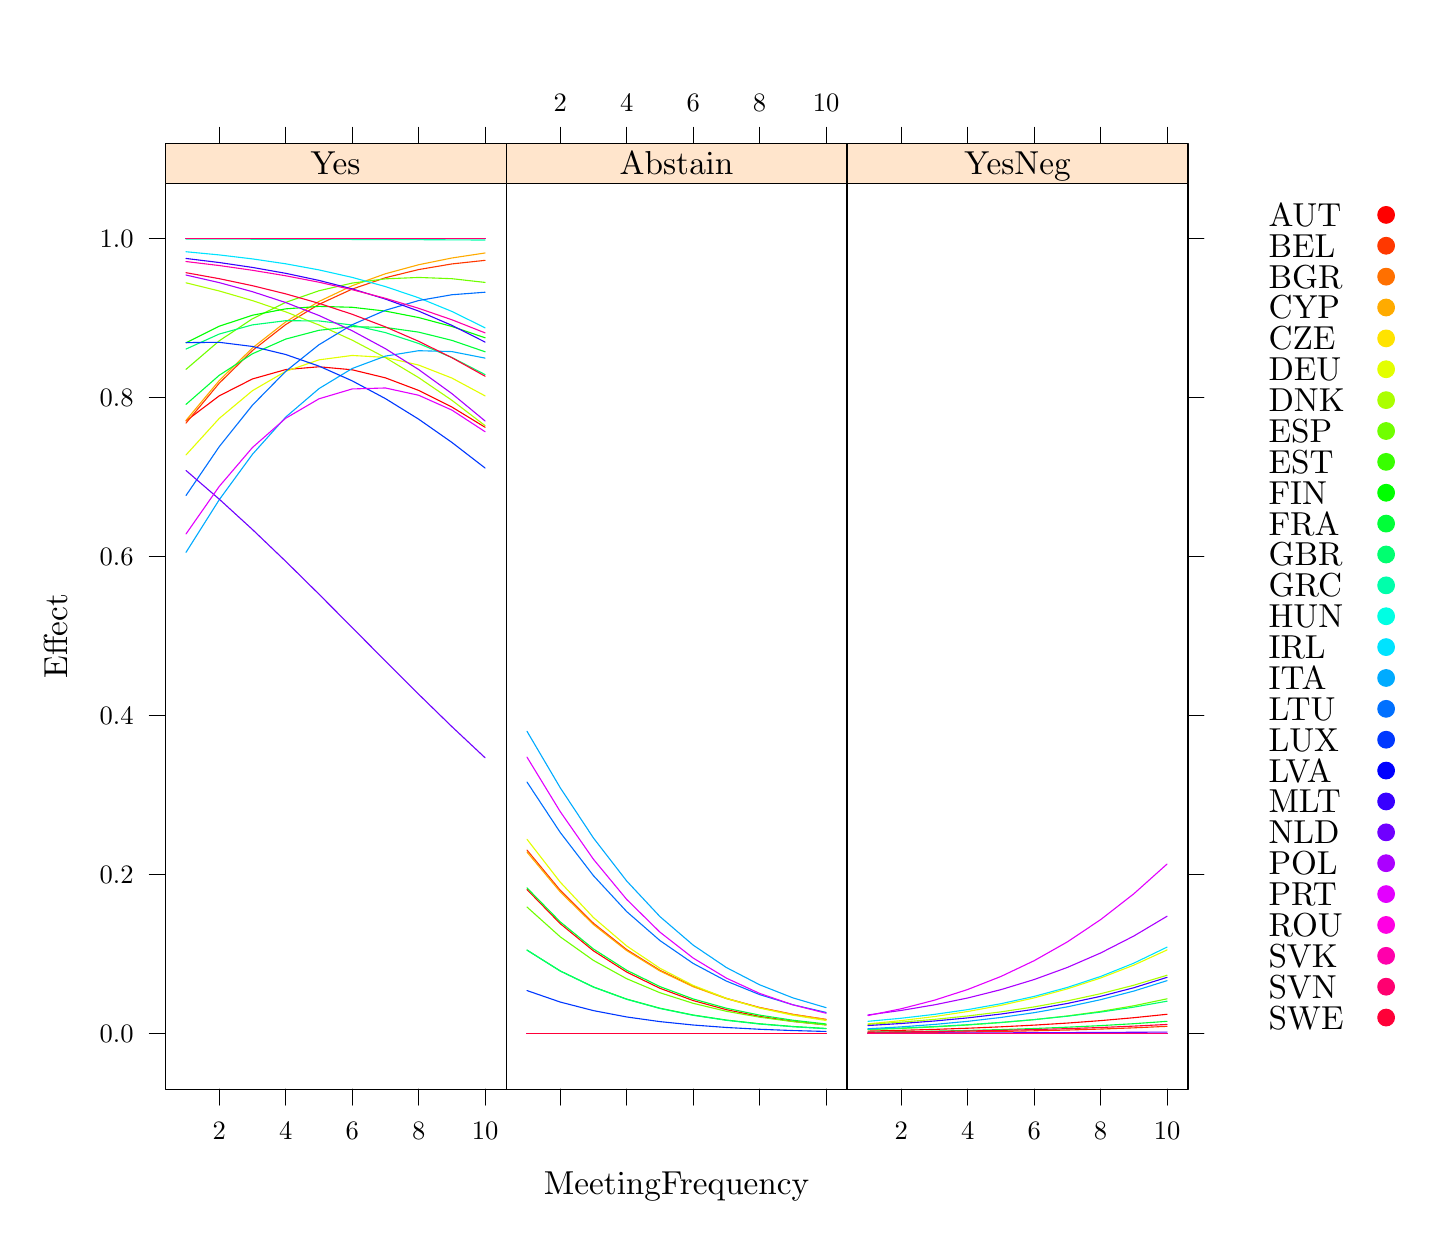
\begin{tikzpicture}[x=1pt,y=1pt]
\definecolor[named]{drawColor}{rgb}{0.00,0.00,0.00}
\definecolor[named]{fillColor}{rgb}{1.00,1.00,1.00}
\fill[color=fillColor,] (0,0) rectangle (505.89,433.62);
\begin{scope}
\path[clip] (  0.00,  0.00) rectangle (505.89,433.62);
\definecolor[named]{fillColor}{rgb}{0.00,0.00,0.00}
\end{scope}
\begin{scope}
\path[clip] (  0.00,  0.00) rectangle (505.89,433.62);
\definecolor[named]{fillColor}{rgb}{0.00,0.00,0.00}

\draw[fill opacity=0.00,draw opacity=0.00,] (  0.00,  0.00) rectangle (505.89,433.62);
\end{scope}
\begin{scope}
\path[clip] (  0.00,  0.00) rectangle (505.89,433.62);
\definecolor[named]{fillColor}{rgb}{0.00,0.00,0.00}
\end{scope}
\begin{scope}
\path[clip] (  0.00,  0.00) rectangle (505.89,433.62);
\definecolor[named]{fillColor}{rgb}{0.00,0.00,0.00}
\definecolor[named]{drawColor}{rgb}{0.00,0.00,0.00}

\node[color=drawColor,anchor=base,inner sep=0pt, outer sep=0pt, scale=  1.20] at (234.47, 12.04) {MeetingFrequency%
};
\end{scope}
\begin{scope}
\path[clip] (  0.00,  0.00) rectangle (505.89,433.62);
\definecolor[named]{fillColor}{rgb}{0.00,0.00,0.00}
\definecolor[named]{drawColor}{rgb}{0.00,0.00,0.00}

\node[rotate= 90.00,color=drawColor,anchor=base,inner sep=0pt, outer sep=0pt, scale=  1.20] at ( 14.29,213.72) {Effect%
};
\end{scope}
\begin{scope}
\path[clip] (  0.00,  0.00) rectangle (505.89,433.62);
\definecolor[named]{fillColor}{rgb}{0.00,0.00,0.00}
\end{scope}
\begin{scope}
\path[clip] (  0.00,  0.00) rectangle (505.89,433.62);
\definecolor[named]{fillColor}{rgb}{0.00,0.00,0.00}
\end{scope}
\begin{scope}
\path[clip] (  0.00,  0.00) rectangle (505.89,433.62);
\definecolor[named]{fillColor}{rgb}{0.00,0.00,0.00}
\end{scope}
\begin{scope}
\path[clip] ( 49.65, 50.02) rectangle (172.86,377.42);
\definecolor[named]{fillColor}{rgb}{0.00,0.00,0.00}
\end{scope}
\begin{scope}
\path[clip] (  0.00,  0.00) rectangle (505.89,433.62);
\definecolor[named]{fillColor}{rgb}{0.00,0.00,0.00}
\end{scope}
\begin{scope}
\path[clip] (  0.00,  0.00) rectangle (505.89,433.62);
\definecolor[named]{fillColor}{rgb}{0.00,0.00,0.00}
\definecolor[named]{drawColor}{rgb}{0.00,0.00,0.00}

\draw[color=drawColor,line cap=round,line join=round,fill opacity=0.00,] ( 69.22,391.87) -- ( 69.22,397.56);

\draw[color=drawColor,line cap=round,line join=round,fill opacity=0.00,] ( 93.24,391.87) -- ( 93.24,397.56);

\draw[color=drawColor,line cap=round,line join=round,fill opacity=0.00,] (117.26,391.87) -- (117.26,397.56);

\draw[color=drawColor,line cap=round,line join=round,fill opacity=0.00,] (141.28,391.87) -- (141.28,397.56);

\draw[color=drawColor,line cap=round,line join=round,fill opacity=0.00,] (165.29,391.87) -- (165.29,397.56);
\end{scope}
\begin{scope}
\path[clip] (  0.00,  0.00) rectangle (505.89,433.62);
\definecolor[named]{fillColor}{rgb}{0.00,0.00,0.00}
\end{scope}
\begin{scope}
\path[clip] (  0.00,  0.00) rectangle (505.89,433.62);
\definecolor[named]{fillColor}{rgb}{0.00,0.00,0.00}
\definecolor[named]{drawColor}{rgb}{0.00,0.00,0.00}

\draw[color=drawColor,line cap=round,line join=round,fill opacity=0.00,] ( 49.65, 70.12) -- ( 43.95, 70.12);

\draw[color=drawColor,line cap=round,line join=round,fill opacity=0.00,] ( 49.65,127.56) -- ( 43.95,127.56);

\draw[color=drawColor,line cap=round,line join=round,fill opacity=0.00,] ( 49.65,185.00) -- ( 43.95,185.00);

\draw[color=drawColor,line cap=round,line join=round,fill opacity=0.00,] ( 49.65,242.43) -- ( 43.95,242.43);

\draw[color=drawColor,line cap=round,line join=round,fill opacity=0.00,] ( 49.65,299.87) -- ( 43.95,299.87);

\draw[color=drawColor,line cap=round,line join=round,fill opacity=0.00,] ( 49.65,357.31) -- ( 43.95,357.31);

\node[color=drawColor,anchor=base east,inner sep=0pt, outer sep=0pt, scale=  0.96] at ( 38.26, 66.81) {0.0%
};

\node[color=drawColor,anchor=base east,inner sep=0pt, outer sep=0pt, scale=  0.96] at ( 38.26,124.25) {0.2%
};

\node[color=drawColor,anchor=base east,inner sep=0pt, outer sep=0pt, scale=  0.96] at ( 38.26,181.69) {0.4%
};

\node[color=drawColor,anchor=base east,inner sep=0pt, outer sep=0pt, scale=  0.96] at ( 38.26,239.13) {0.6%
};

\node[color=drawColor,anchor=base east,inner sep=0pt, outer sep=0pt, scale=  0.96] at ( 38.26,296.57) {0.8%
};

\node[color=drawColor,anchor=base east,inner sep=0pt, outer sep=0pt, scale=  0.96] at ( 38.26,354.01) {1.0%
};
\end{scope}
\begin{scope}
\path[clip] (  0.00,  0.00) rectangle (505.89,433.62);
\definecolor[named]{fillColor}{rgb}{0.00,0.00,0.00}
\end{scope}
\begin{scope}
\path[clip] (  0.00,  0.00) rectangle (505.89,433.62);
\definecolor[named]{fillColor}{rgb}{0.00,0.00,0.00}
\definecolor[named]{drawColor}{rgb}{0.00,0.00,0.00}

\draw[color=drawColor,line cap=round,line join=round,fill opacity=0.00,] ( 69.22, 50.02) -- ( 69.22, 44.32);

\draw[color=drawColor,line cap=round,line join=round,fill opacity=0.00,] ( 93.24, 50.02) -- ( 93.24, 44.32);

\draw[color=drawColor,line cap=round,line join=round,fill opacity=0.00,] (117.26, 50.02) -- (117.26, 44.32);

\draw[color=drawColor,line cap=round,line join=round,fill opacity=0.00,] (141.28, 50.02) -- (141.28, 44.32);

\draw[color=drawColor,line cap=round,line join=round,fill opacity=0.00,] (165.29, 50.02) -- (165.29, 44.32);

\node[color=drawColor,anchor=base,inner sep=0pt, outer sep=0pt, scale=  0.96] at ( 69.22, 32.02) {2%
};

\node[color=drawColor,anchor=base,inner sep=0pt, outer sep=0pt, scale=  0.96] at ( 93.24, 32.02) {4%
};

\node[color=drawColor,anchor=base,inner sep=0pt, outer sep=0pt, scale=  0.96] at (117.26, 32.02) {6%
};

\node[color=drawColor,anchor=base,inner sep=0pt, outer sep=0pt, scale=  0.96] at (141.28, 32.02) {8%
};

\node[color=drawColor,anchor=base,inner sep=0pt, outer sep=0pt, scale=  0.96] at (165.29, 32.02) {10%
};
\end{scope}
\begin{scope}
\path[clip] (  0.00,  0.00) rectangle (505.89,433.62);
\definecolor[named]{fillColor}{rgb}{0.00,0.00,0.00}
\end{scope}
\begin{scope}
\path[clip] ( 49.65, 50.02) rectangle (172.86,377.42);
\definecolor[named]{fillColor}{rgb}{0.00,0.00,0.00}
\definecolor[named]{drawColor}{rgb}{1.00,0.00,0.00}

\draw[color=drawColor,line cap=round,line join=round,fill opacity=0.00,] ( 57.21,291.51) --
	( 69.22,300.58) --
	( 81.23,306.68) --
	( 93.24,310.07) --
	(105.25,311.08) --
	(117.26,309.99) --
	(129.27,307.08) --
	(141.28,302.54) --
	(153.28,296.54) --
	(165.29,289.22);
\definecolor[named]{drawColor}{rgb}{1.00,0.22,0.00}

\draw[color=drawColor,line cap=round,line join=round,fill opacity=0.00,] ( 57.21,290.72) --
	( 69.22,305.15) --
	( 81.23,316.95) --
	( 93.24,326.34) --
	(105.25,333.63) --
	(117.26,339.16) --
	(129.27,343.26) --
	(141.28,346.21) --
	(153.28,348.24) --
	(165.29,349.54);
\definecolor[named]{drawColor}{rgb}{1.00,0.44,0.00}

\draw[color=drawColor,line cap=round,line join=round,fill opacity=0.00,] ( 57.21,357.31) --
	( 69.22,357.31) --
	( 81.23,357.31) --
	( 93.24,357.31) --
	(105.25,357.31) --
	(117.26,357.31) --
	(129.27,357.31) --
	(141.28,357.31) --
	(153.28,357.31) --
	(165.29,357.31);
\definecolor[named]{drawColor}{rgb}{1.00,0.67,0.00}

\draw[color=drawColor,line cap=round,line join=round,fill opacity=0.00,] ( 57.21,291.71) --
	( 69.22,306.09) --
	( 81.23,317.89) --
	( 93.24,327.31) --
	(105.25,334.68) --
	(117.26,340.37) --
	(129.27,344.69) --
	(141.28,347.95) --
	(153.28,350.39) --
	(165.29,352.20);
\definecolor[named]{drawColor}{rgb}{1.00,0.89,0.00}

\draw[color=drawColor,line cap=round,line join=round,fill opacity=0.00,] ( 57.21,357.31) --
	( 69.22,357.31) --
	( 81.23,357.31) --
	( 93.24,357.31) --
	(105.25,357.31) --
	(117.26,357.31) --
	(129.27,357.31) --
	(141.28,357.31) --
	(153.28,357.31) --
	(165.29,357.31);
\definecolor[named]{drawColor}{rgb}{0.89,1.00,0.00}

\draw[color=drawColor,line cap=round,line join=round,fill opacity=0.00,] ( 57.21,279.22) --
	( 69.22,292.42) --
	( 81.23,302.45) --
	( 93.24,309.43) --
	(105.25,313.58) --
	(117.26,315.17) --
	(129.27,314.47) --
	(141.28,311.70) --
	(153.28,307.01) --
	(165.29,300.56);
\definecolor[named]{drawColor}{rgb}{0.67,1.00,0.00}

\draw[color=drawColor,line cap=round,line join=round,fill opacity=0.00,] ( 57.21,341.42) --
	( 69.22,338.47) --
	( 81.23,334.99) --
	( 93.24,330.93) --
	(105.25,326.19) --
	(117.26,320.70) --
	(129.27,314.38) --
	(141.28,307.16) --
	(153.28,298.98) --
	(165.29,289.81);
\definecolor[named]{drawColor}{rgb}{0.44,1.00,0.00}

\draw[color=drawColor,line cap=round,line join=round,fill opacity=0.00,] ( 57.21,310.14) --
	( 69.22,320.46) --
	( 81.23,328.43) --
	( 93.24,334.35) --
	(105.25,338.55) --
	(117.26,341.32) --
	(129.27,342.86) --
	(141.28,343.36) --
	(153.28,342.91) --
	(165.29,341.56);
\definecolor[named]{drawColor}{rgb}{0.22,1.00,0.00}

\draw[color=drawColor,line cap=round,line join=round,fill opacity=0.00,] ( 57.21,357.31) --
	( 69.22,357.31) --
	( 81.23,357.31) --
	( 93.24,357.31) --
	(105.25,357.31) --
	(117.26,357.31) --
	(129.27,357.31) --
	(141.28,357.31) --
	(153.28,357.31) --
	(165.29,357.31);
\definecolor[named]{drawColor}{rgb}{0.00,1.00,0.00}

\draw[color=drawColor,line cap=round,line join=round,fill opacity=0.00,] ( 57.21,319.76) --
	( 69.22,325.73) --
	( 81.23,329.71) --
	( 93.24,332.01) --
	(105.25,332.90) --
	(117.26,332.58) --
	(129.27,331.20) --
	(141.28,328.87) --
	(153.28,325.65) --
	(165.29,321.56);
\definecolor[named]{drawColor}{rgb}{0.00,1.00,0.22}

\draw[color=drawColor,line cap=round,line join=round,fill opacity=0.00,] ( 57.21,297.48) --
	( 69.22,308.00) --
	( 81.23,315.78) --
	( 93.24,321.09) --
	(105.25,324.26) --
	(117.26,325.58) --
	(129.27,325.29) --
	(141.28,323.60) --
	(153.28,320.63) --
	(165.29,316.50);
\definecolor[named]{drawColor}{rgb}{0.00,1.00,0.44}

\draw[color=drawColor,line cap=round,line join=round,fill opacity=0.00,] ( 57.21,317.48) --
	( 69.22,322.91) --
	( 81.23,326.23) --
	( 93.24,327.73) --
	(105.25,327.65) --
	(117.26,326.17) --
	(129.27,323.43) --
	(141.28,319.50) --
	(153.28,314.44) --
	(165.29,308.26);
\definecolor[named]{drawColor}{rgb}{0.00,1.00,0.67}

\draw[color=drawColor,line cap=round,line join=round,fill opacity=0.00,] ( 57.21,357.22) --
	( 69.22,357.20) --
	( 81.23,357.18) --
	( 93.24,357.16) --
	(105.25,357.13) --
	(117.26,357.09) --
	(129.27,357.05) --
	(141.28,357.01) --
	(153.28,356.95) --
	(165.29,356.88);
\definecolor[named]{drawColor}{rgb}{0.00,1.00,0.89}

\draw[color=drawColor,line cap=round,line join=round,fill opacity=0.00,] ( 57.21,357.31) --
	( 69.22,357.31) --
	( 81.23,357.31) --
	( 93.24,357.31) --
	(105.25,357.31) --
	(117.26,357.31) --
	(129.27,357.31) --
	(141.28,357.31) --
	(153.28,357.31) --
	(165.29,357.31);
\definecolor[named]{drawColor}{rgb}{0.00,0.89,1.00}

\draw[color=drawColor,line cap=round,line join=round,fill opacity=0.00,] ( 57.21,352.65) --
	( 69.22,351.50) --
	( 81.23,350.06) --
	( 93.24,348.29) --
	(105.25,346.09) --
	(117.26,343.38) --
	(129.27,340.06) --
	(141.28,336.00) --
	(153.28,331.08) --
	(165.29,325.16);
\definecolor[named]{drawColor}{rgb}{0.00,0.67,1.00}

\draw[color=drawColor,line cap=round,line join=round,fill opacity=0.00,] ( 57.21,244.02) --
	( 69.22,263.03) --
	( 81.23,279.46) --
	( 93.24,292.89) --
	(105.25,303.18) --
	(117.26,310.46) --
	(129.27,314.94) --
	(141.28,316.89) --
	(153.28,316.57) --
	(165.29,314.21);
\definecolor[named]{drawColor}{rgb}{0.00,0.44,1.00}

\draw[color=drawColor,line cap=round,line join=round,fill opacity=0.00,] ( 57.21,264.55) --
	( 69.22,282.21) --
	( 81.23,297.21) --
	( 93.24,309.44) --
	(105.25,319.04) --
	(117.26,326.28) --
	(129.27,331.50) --
	(141.28,335.01) --
	(153.28,337.11) --
	(165.29,338.02);
\definecolor[named]{drawColor}{rgb}{0.00,0.22,1.00}

\draw[color=drawColor,line cap=round,line join=round,fill opacity=0.00,] ( 57.21,319.81) --
	( 69.22,319.92) --
	( 81.23,318.42) --
	( 93.24,315.51) --
	(105.25,311.33) --
	(117.26,306.00) --
	(129.27,299.58) --
	(141.28,292.15) --
	(153.28,283.76) --
	(165.29,274.49);
\definecolor[named]{drawColor}{rgb}{0.00,0.00,1.00}

\draw[color=drawColor,line cap=round,line join=round,fill opacity=0.00,] ( 57.21,357.31) --
	( 69.22,357.31) --
	( 81.23,357.31) --
	( 93.24,357.31) --
	(105.25,357.31) --
	(117.26,357.31) --
	(129.27,357.31) --
	(141.28,357.31) --
	(153.28,357.31) --
	(165.29,357.31);
\definecolor[named]{drawColor}{rgb}{0.22,0.00,1.00}

\draw[color=drawColor,line cap=round,line join=round,fill opacity=0.00,] ( 57.21,350.22) --
	( 69.22,348.75) --
	( 81.23,346.98) --
	( 93.24,344.85) --
	(105.25,342.29) --
	(117.26,339.22) --
	(129.27,335.55) --
	(141.28,331.20) --
	(153.28,326.05) --
	(165.29,320.01);
\definecolor[named]{drawColor}{rgb}{0.44,0.00,1.00}

\draw[color=drawColor,line cap=round,line join=round,fill opacity=0.00,] ( 57.21,273.61) --
	( 69.22,263.25) --
	( 81.23,252.27) --
	( 93.24,240.78) --
	(105.25,228.93) --
	(117.26,216.85) --
	(129.27,204.74) --
	(141.28,192.75) --
	(153.28,181.05) --
	(165.29,169.79);
\definecolor[named]{drawColor}{rgb}{0.67,0.00,1.00}

\draw[color=drawColor,line cap=round,line join=round,fill opacity=0.00,] ( 57.21,344.23) --
	( 69.22,341.49) --
	( 81.23,338.21) --
	( 93.24,334.29) --
	(105.25,329.62) --
	(117.26,324.10) --
	(129.27,317.62) --
	(141.28,310.08) --
	(153.28,301.39) --
	(165.29,291.49);
\definecolor[named]{drawColor}{rgb}{0.89,0.00,1.00}

\draw[color=drawColor,line cap=round,line join=round,fill opacity=0.00,] ( 57.21,250.66) --
	( 69.22,267.85) --
	( 81.23,281.91) --
	( 93.24,292.48) --
	(105.25,299.50) --
	(117.26,303.07) --
	(129.27,303.42) --
	(141.28,300.79) --
	(153.28,295.44) --
	(165.29,287.61);
\definecolor[named]{drawColor}{rgb}{1.00,0.00,0.89}

\draw[color=drawColor,line cap=round,line join=round,fill opacity=0.00,] ( 57.21,357.31) --
	( 69.22,357.31) --
	( 81.23,357.31) --
	( 93.24,357.31) --
	(105.25,357.31) --
	(117.26,357.31) --
	(129.27,357.31) --
	(141.28,357.31) --
	(153.28,357.31) --
	(165.29,357.31);
\definecolor[named]{drawColor}{rgb}{1.00,0.00,0.67}

\draw[color=drawColor,line cap=round,line join=round,fill opacity=0.00,] ( 57.21,349.11) --
	( 69.22,347.66) --
	( 81.23,345.95) --
	( 93.24,343.96) --
	(105.25,341.64) --
	(117.26,338.94) --
	(129.27,335.82) --
	(141.28,332.21) --
	(153.28,328.07) --
	(165.29,323.33);
\definecolor[named]{drawColor}{rgb}{1.00,0.00,0.44}

\draw[color=drawColor,line cap=round,line join=round,fill opacity=0.00,] ( 57.21,357.31) --
	( 69.22,357.31) --
	( 81.23,357.31) --
	( 93.24,357.31) --
	(105.25,357.31) --
	(117.26,357.31) --
	(129.27,357.31) --
	(141.28,357.31) --
	(153.28,357.31) --
	(165.29,357.31);
\definecolor[named]{drawColor}{rgb}{1.00,0.00,0.22}

\draw[color=drawColor,line cap=round,line join=round,fill opacity=0.00,] ( 57.21,345.08) --
	( 69.22,342.91) --
	( 81.23,340.38) --
	( 93.24,337.43) --
	(105.25,334.01) --
	(117.26,330.05) --
	(129.27,325.50) --
	(141.28,320.29) --
	(153.28,314.37) --
	(165.29,307.67);
\end{scope}
\begin{scope}
\path[clip] (  0.00,  0.00) rectangle (505.89,433.62);
\definecolor[named]{fillColor}{rgb}{0.00,0.00,0.00}
\end{scope}
\begin{scope}
\path[clip] (  0.00,  0.00) rectangle (505.89,433.62);
\definecolor[named]{fillColor}{rgb}{0.00,0.00,0.00}
\definecolor[named]{drawColor}{rgb}{0.00,0.00,0.00}

\draw[color=drawColor,line cap=round,line join=round,fill opacity=0.00,] ( 49.65, 50.02) rectangle (172.86,377.42);
\end{scope}
\begin{scope}
\path[clip] (  0.00,  0.00) rectangle (505.89,433.62);
\definecolor[named]{fillColor}{rgb}{0.00,0.00,0.00}
\end{scope}
\begin{scope}
\path[clip] (  0.00,  0.00) rectangle (505.89,433.62);
\definecolor[named]{fillColor}{rgb}{0.00,0.00,0.00}
\end{scope}
\begin{scope}
\path[clip] ( 49.65,377.42) rectangle (172.86,391.87);
\definecolor[named]{fillColor}{rgb}{0.00,0.00,0.00}
\definecolor[named]{drawColor}{rgb}{1.00,0.90,0.80}
\definecolor[named]{fillColor}{rgb}{1.00,0.90,0.80}

\draw[color=drawColor,line cap=round,line join=round,fill=fillColor,] ( 49.65,377.42) rectangle (172.86,391.87);
\definecolor[named]{drawColor}{rgb}{0.00,0.00,0.00}

\node[color=drawColor,anchor=base west,inner sep=0pt, outer sep=0pt, scale=  1.20] at (102.22,380.51) {Yes%
};
\end{scope}
\begin{scope}
\path[clip] (  0.00,  0.00) rectangle (505.89,433.62);
\definecolor[named]{fillColor}{rgb}{0.00,0.00,0.00}
\end{scope}
\begin{scope}
\path[clip] (  0.00,  0.00) rectangle (505.89,433.62);
\definecolor[named]{fillColor}{rgb}{0.00,0.00,0.00}
\definecolor[named]{drawColor}{rgb}{0.00,0.00,0.00}

\draw[color=drawColor,line cap=round,line join=round,fill opacity=0.00,] ( 49.65,377.42) rectangle (172.86,391.87);
\end{scope}
\begin{scope}
\path[clip] (  0.00,  0.00) rectangle (505.89,433.62);
\definecolor[named]{fillColor}{rgb}{0.00,0.00,0.00}
\end{scope}
\begin{scope}
\path[clip] (  0.00,  0.00) rectangle (505.89,433.62);
\definecolor[named]{fillColor}{rgb}{0.00,0.00,0.00}
\end{scope}
\begin{scope}
\path[clip] (172.86, 50.02) rectangle (296.07,377.42);
\definecolor[named]{fillColor}{rgb}{0.00,0.00,0.00}
\end{scope}
\begin{scope}
\path[clip] (  0.00,  0.00) rectangle (505.89,433.62);
\definecolor[named]{fillColor}{rgb}{0.00,0.00,0.00}
\end{scope}
\begin{scope}
\path[clip] (  0.00,  0.00) rectangle (505.89,433.62);
\definecolor[named]{fillColor}{rgb}{0.00,0.00,0.00}
\definecolor[named]{drawColor}{rgb}{0.00,0.00,0.00}

\draw[color=drawColor,line cap=round,line join=round,fill opacity=0.00,] (192.43,391.87) -- (192.43,397.56);

\draw[color=drawColor,line cap=round,line join=round,fill opacity=0.00,] (216.45,391.87) -- (216.45,397.56);

\draw[color=drawColor,line cap=round,line join=round,fill opacity=0.00,] (240.47,391.87) -- (240.47,397.56);

\draw[color=drawColor,line cap=round,line join=round,fill opacity=0.00,] (264.49,391.87) -- (264.49,397.56);

\draw[color=drawColor,line cap=round,line join=round,fill opacity=0.00,] (288.51,391.87) -- (288.51,397.56);

\node[color=drawColor,anchor=base,inner sep=0pt, outer sep=0pt, scale=  0.96] at (192.43,403.25) {2%
};

\node[color=drawColor,anchor=base,inner sep=0pt, outer sep=0pt, scale=  0.96] at (216.45,403.25) {4%
};

\node[color=drawColor,anchor=base,inner sep=0pt, outer sep=0pt, scale=  0.96] at (240.47,403.25) {6%
};

\node[color=drawColor,anchor=base,inner sep=0pt, outer sep=0pt, scale=  0.96] at (264.49,403.25) {8%
};

\node[color=drawColor,anchor=base,inner sep=0pt, outer sep=0pt, scale=  0.96] at (288.51,403.25) {10%
};
\end{scope}
\begin{scope}
\path[clip] (  0.00,  0.00) rectangle (505.89,433.62);
\definecolor[named]{fillColor}{rgb}{0.00,0.00,0.00}
\end{scope}
\begin{scope}
\path[clip] (  0.00,  0.00) rectangle (505.89,433.62);
\definecolor[named]{fillColor}{rgb}{0.00,0.00,0.00}
\end{scope}
\begin{scope}
\path[clip] (  0.00,  0.00) rectangle (505.89,433.62);
\definecolor[named]{fillColor}{rgb}{0.00,0.00,0.00}
\end{scope}
\begin{scope}
\path[clip] (  0.00,  0.00) rectangle (505.89,433.62);
\definecolor[named]{fillColor}{rgb}{0.00,0.00,0.00}
\definecolor[named]{drawColor}{rgb}{0.00,0.00,0.00}

\draw[color=drawColor,line cap=round,line join=round,fill opacity=0.00,] (192.43, 50.02) -- (192.43, 44.32);

\draw[color=drawColor,line cap=round,line join=round,fill opacity=0.00,] (216.45, 50.02) -- (216.45, 44.32);

\draw[color=drawColor,line cap=round,line join=round,fill opacity=0.00,] (240.47, 50.02) -- (240.47, 44.32);

\draw[color=drawColor,line cap=round,line join=round,fill opacity=0.00,] (264.49, 50.02) -- (264.49, 44.32);

\draw[color=drawColor,line cap=round,line join=round,fill opacity=0.00,] (288.51, 50.02) -- (288.51, 44.32);
\end{scope}
\begin{scope}
\path[clip] (  0.00,  0.00) rectangle (505.89,433.62);
\definecolor[named]{fillColor}{rgb}{0.00,0.00,0.00}
\end{scope}
\begin{scope}
\path[clip] (172.86, 50.02) rectangle (296.07,377.42);
\definecolor[named]{fillColor}{rgb}{0.00,0.00,0.00}
\definecolor[named]{drawColor}{rgb}{1.00,0.00,0.00}

\draw[color=drawColor,line cap=round,line join=round,fill opacity=0.00,] (180.42,122.20) --
	(192.43,109.87) --
	(204.44,100.03) --
	(216.45, 92.36) --
	(228.46, 86.50) --
	(240.47, 82.07) --
	(252.48, 78.77) --
	(264.49, 76.34) --
	(276.50, 74.56) --
	(288.51, 73.27);
\definecolor[named]{drawColor}{rgb}{1.00,0.22,0.00}

\draw[color=drawColor,line cap=round,line join=round,fill opacity=0.00,] (180.42,136.45) --
	(192.43,121.93) --
	(204.44,110.01) --
	(216.45,100.48) --
	(228.46, 93.01) --
	(240.47, 87.25) --
	(252.48, 82.87) --
	(264.49, 79.57) --
	(276.50, 77.10) --
	(288.51, 75.26);
\definecolor[named]{drawColor}{rgb}{1.00,0.44,0.00}

\draw[color=drawColor,line cap=round,line join=round,fill opacity=0.00,] (180.42, 70.12) --
	(192.43, 70.12) --
	(204.44, 70.12) --
	(216.45, 70.12) --
	(228.46, 70.12) --
	(240.47, 70.12) --
	(252.48, 70.12) --
	(264.49, 70.12) --
	(276.50, 70.12) --
	(288.51, 70.12);
\definecolor[named]{drawColor}{rgb}{1.00,0.67,0.00}

\draw[color=drawColor,line cap=round,line join=round,fill opacity=0.00,] (180.42,135.72) --
	(192.43,121.34) --
	(204.44,109.54) --
	(216.45,100.12) --
	(228.46, 92.75) --
	(240.47, 87.06) --
	(252.48, 82.74) --
	(264.49, 79.48) --
	(276.50, 77.04) --
	(288.51, 75.23);
\definecolor[named]{drawColor}{rgb}{1.00,0.89,0.00}

\draw[color=drawColor,line cap=round,line join=round,fill opacity=0.00,] (180.42, 70.12) --
	(192.43, 70.12) --
	(204.44, 70.12) --
	(216.45, 70.12) --
	(228.46, 70.12) --
	(240.47, 70.12) --
	(252.48, 70.12) --
	(264.49, 70.12) --
	(276.50, 70.12) --
	(288.51, 70.12);
\definecolor[named]{drawColor}{rgb}{0.89,1.00,0.00}

\draw[color=drawColor,line cap=round,line join=round,fill opacity=0.00,] (180.42,140.36) --
	(192.43,124.87) --
	(204.44,112.07) --
	(216.45,101.80) --
	(228.46, 93.75) --
	(240.47, 87.55) --
	(252.48, 82.87) --
	(264.49, 79.36) --
	(276.50, 76.76) --
	(288.51, 74.86);
\definecolor[named]{drawColor}{rgb}{0.67,1.00,0.00}

\draw[color=drawColor,line cap=round,line join=round,fill opacity=0.00,] (180.42, 70.12) --
	(192.43, 70.12) --
	(204.44, 70.12) --
	(216.45, 70.12) --
	(228.46, 70.12) --
	(240.47, 70.12) --
	(252.48, 70.12) --
	(264.49, 70.12) --
	(276.50, 70.12) --
	(288.51, 70.12);
\definecolor[named]{drawColor}{rgb}{0.44,1.00,0.00}

\draw[color=drawColor,line cap=round,line join=round,fill opacity=0.00,] (180.42,115.87) --
	(192.43,105.10) --
	(204.44, 96.58) --
	(216.45, 89.96) --
	(228.46, 84.90) --
	(240.47, 81.07) --
	(252.48, 78.19) --
	(264.49, 76.05) --
	(276.50, 74.46) --
	(288.51, 73.28);
\definecolor[named]{drawColor}{rgb}{0.22,1.00,0.00}

\draw[color=drawColor,line cap=round,line join=round,fill opacity=0.00,] (180.42, 70.12) --
	(192.43, 70.12) --
	(204.44, 70.12) --
	(216.45, 70.12) --
	(228.46, 70.12) --
	(240.47, 70.12) --
	(252.48, 70.12) --
	(264.49, 70.12) --
	(276.50, 70.12) --
	(288.51, 70.12);
\definecolor[named]{drawColor}{rgb}{0.00,1.00,0.00}

\draw[color=drawColor,line cap=round,line join=round,fill opacity=0.00,] (180.42,100.30) --
	(192.43, 92.78) --
	(204.44, 86.99) --
	(216.45, 82.60) --
	(228.46, 79.30) --
	(240.47, 76.84) --
	(252.48, 75.02) --
	(264.49, 73.68) --
	(276.50, 72.70) --
	(288.51, 71.98);
\definecolor[named]{drawColor}{rgb}{0.00,1.00,0.22}

\draw[color=drawColor,line cap=round,line join=round,fill opacity=0.00,] (180.42,122.78) --
	(192.43,110.51) --
	(204.44,100.70) --
	(216.45, 93.02) --
	(228.46, 87.12) --
	(240.47, 82.65) --
	(252.48, 79.30) --
	(264.49, 76.80) --
	(276.50, 74.96) --
	(288.51, 73.61);
\definecolor[named]{drawColor}{rgb}{0.00,1.00,0.44}

\draw[color=drawColor,line cap=round,line join=round,fill opacity=0.00,] (180.42,100.31) --
	(192.43, 92.74) --
	(204.44, 86.92) --
	(216.45, 82.51) --
	(228.46, 79.20) --
	(240.47, 76.74) --
	(252.48, 74.92) --
	(264.49, 73.58) --
	(276.50, 72.61) --
	(288.51, 71.90);
\definecolor[named]{drawColor}{rgb}{0.00,1.00,0.67}

\draw[color=drawColor,line cap=round,line join=round,fill opacity=0.00,] (180.42, 70.12) --
	(192.43, 70.12) --
	(204.44, 70.12) --
	(216.45, 70.12) --
	(228.46, 70.12) --
	(240.47, 70.12) --
	(252.48, 70.12) --
	(264.49, 70.12) --
	(276.50, 70.12) --
	(288.51, 70.12);
\definecolor[named]{drawColor}{rgb}{0.00,1.00,0.89}

\draw[color=drawColor,line cap=round,line join=round,fill opacity=0.00,] (180.42, 70.12) --
	(192.43, 70.12) --
	(204.44, 70.12) --
	(216.45, 70.12) --
	(228.46, 70.12) --
	(240.47, 70.12) --
	(252.48, 70.12) --
	(264.49, 70.12) --
	(276.50, 70.12) --
	(288.51, 70.12);
\definecolor[named]{drawColor}{rgb}{0.00,0.89,1.00}

\draw[color=drawColor,line cap=round,line join=round,fill opacity=0.00,] (180.42, 70.12) --
	(192.43, 70.12) --
	(204.44, 70.12) --
	(216.45, 70.12) --
	(228.46, 70.12) --
	(240.47, 70.12) --
	(252.48, 70.12) --
	(264.49, 70.12) --
	(276.50, 70.12) --
	(288.51, 70.12);
\definecolor[named]{drawColor}{rgb}{0.00,0.67,1.00}

\draw[color=drawColor,line cap=round,line join=round,fill opacity=0.00,] (180.42,179.38) --
	(192.43,158.98) --
	(204.44,140.81) --
	(216.45,125.27) --
	(228.46,112.42) --
	(240.47,102.10) --
	(252.48, 94.00) --
	(264.49, 87.77) --
	(276.50, 83.04) --
	(288.51, 79.50);
\definecolor[named]{drawColor}{rgb}{0.00,0.44,1.00}

\draw[color=drawColor,line cap=round,line join=round,fill opacity=0.00,] (180.42,161.04) --
	(192.43,142.83) --
	(204.44,127.20) --
	(216.45,114.22) --
	(228.46,103.75) --
	(240.47, 95.49) --
	(252.48, 89.10) --
	(264.49, 84.22) --
	(276.50, 80.54) --
	(288.51, 77.78);
\definecolor[named]{drawColor}{rgb}{0.00,0.22,1.00}

\draw[color=drawColor,line cap=round,line join=round,fill opacity=0.00,] (180.42, 85.68) --
	(192.43, 81.53) --
	(204.44, 78.43) --
	(216.45, 76.14) --
	(228.46, 74.46) --
	(240.47, 73.23) --
	(252.48, 72.34) --
	(264.49, 71.69) --
	(276.50, 71.23) --
	(288.51, 70.90);
\definecolor[named]{drawColor}{rgb}{0.00,0.00,1.00}

\draw[color=drawColor,line cap=round,line join=round,fill opacity=0.00,] (180.42, 70.12) --
	(192.43, 70.12) --
	(204.44, 70.12) --
	(216.45, 70.12) --
	(228.46, 70.12) --
	(240.47, 70.12) --
	(252.48, 70.12) --
	(264.49, 70.12) --
	(276.50, 70.12) --
	(288.51, 70.12);
\definecolor[named]{drawColor}{rgb}{0.22,0.00,1.00}

\draw[color=drawColor,line cap=round,line join=round,fill opacity=0.00,] (180.42, 70.12) --
	(192.43, 70.12) --
	(204.44, 70.12) --
	(216.45, 70.12) --
	(228.46, 70.12) --
	(240.47, 70.12) --
	(252.48, 70.12) --
	(264.49, 70.12) --
	(276.50, 70.12) --
	(288.51, 70.12);
\definecolor[named]{drawColor}{rgb}{0.44,0.00,1.00}

\draw[color=drawColor,line cap=round,line join=round,fill opacity=0.00,] (180.42, 70.12) --
	(192.43, 70.12) --
	(204.44, 70.12) --
	(216.45, 70.12) --
	(228.46, 70.12) --
	(240.47, 70.12) --
	(252.48, 70.12) --
	(264.49, 70.12) --
	(276.50, 70.12) --
	(288.51, 70.12);
\definecolor[named]{drawColor}{rgb}{0.67,0.00,1.00}

\draw[color=drawColor,line cap=round,line join=round,fill opacity=0.00,] (180.42, 70.12) --
	(192.43, 70.12) --
	(204.44, 70.12) --
	(216.45, 70.12) --
	(228.46, 70.12) --
	(240.47, 70.12) --
	(252.48, 70.12) --
	(264.49, 70.12) --
	(276.50, 70.12) --
	(288.51, 70.12);
\definecolor[named]{drawColor}{rgb}{0.89,0.00,1.00}

\draw[color=drawColor,line cap=round,line join=round,fill opacity=0.00,] (180.42,170.04) --
	(192.43,150.35) --
	(204.44,133.12) --
	(216.45,118.61) --
	(228.46,106.79) --
	(240.47, 97.43) --
	(252.48, 90.17) --
	(264.49, 84.65) --
	(276.50, 80.53) --
	(288.51, 77.48);
\definecolor[named]{drawColor}{rgb}{1.00,0.00,0.89}

\draw[color=drawColor,line cap=round,line join=round,fill opacity=0.00,] (180.42, 70.12) --
	(192.43, 70.12) --
	(204.44, 70.12) --
	(216.45, 70.12) --
	(228.46, 70.12) --
	(240.47, 70.12) --
	(252.48, 70.12) --
	(264.49, 70.12) --
	(276.50, 70.12) --
	(288.51, 70.12);
\definecolor[named]{drawColor}{rgb}{1.00,0.00,0.67}

\draw[color=drawColor,line cap=round,line join=round,fill opacity=0.00,] (180.42, 70.12) --
	(192.43, 70.12) --
	(204.44, 70.12) --
	(216.45, 70.12) --
	(228.46, 70.12) --
	(240.47, 70.12) --
	(252.48, 70.12) --
	(264.49, 70.12) --
	(276.50, 70.12) --
	(288.51, 70.12);
\definecolor[named]{drawColor}{rgb}{1.00,0.00,0.44}

\draw[color=drawColor,line cap=round,line join=round,fill opacity=0.00,] (180.42, 70.12) --
	(192.43, 70.12) --
	(204.44, 70.12) --
	(216.45, 70.12) --
	(228.46, 70.12) --
	(240.47, 70.12) --
	(252.48, 70.12) --
	(264.49, 70.12) --
	(276.50, 70.12) --
	(288.51, 70.12);
\definecolor[named]{drawColor}{rgb}{1.00,0.00,0.22}

\draw[color=drawColor,line cap=round,line join=round,fill opacity=0.00,] (180.42, 70.12) --
	(192.43, 70.12) --
	(204.44, 70.12) --
	(216.45, 70.12) --
	(228.46, 70.12) --
	(240.47, 70.12) --
	(252.48, 70.12) --
	(264.49, 70.12) --
	(276.50, 70.12) --
	(288.51, 70.12);
\end{scope}
\begin{scope}
\path[clip] (  0.00,  0.00) rectangle (505.89,433.62);
\definecolor[named]{fillColor}{rgb}{0.00,0.00,0.00}
\end{scope}
\begin{scope}
\path[clip] (  0.00,  0.00) rectangle (505.89,433.62);
\definecolor[named]{fillColor}{rgb}{0.00,0.00,0.00}
\definecolor[named]{drawColor}{rgb}{0.00,0.00,0.00}

\draw[color=drawColor,line cap=round,line join=round,fill opacity=0.00,] (172.86, 50.02) rectangle (296.07,377.42);
\end{scope}
\begin{scope}
\path[clip] (  0.00,  0.00) rectangle (505.89,433.62);
\definecolor[named]{fillColor}{rgb}{0.00,0.00,0.00}
\end{scope}
\begin{scope}
\path[clip] (  0.00,  0.00) rectangle (505.89,433.62);
\definecolor[named]{fillColor}{rgb}{0.00,0.00,0.00}
\end{scope}
\begin{scope}
\path[clip] (172.86,377.42) rectangle (296.07,391.87);
\definecolor[named]{fillColor}{rgb}{0.00,0.00,0.00}
\definecolor[named]{drawColor}{rgb}{1.00,0.90,0.80}
\definecolor[named]{fillColor}{rgb}{1.00,0.90,0.80}

\draw[color=drawColor,line cap=round,line join=round,fill=fillColor,] (172.86,377.42) rectangle (296.07,391.87);
\definecolor[named]{drawColor}{rgb}{0.00,0.00,0.00}

\node[color=drawColor,anchor=base west,inner sep=0pt, outer sep=0pt, scale=  1.20] at (213.94,380.51) {Abstain%
};
\end{scope}
\begin{scope}
\path[clip] (  0.00,  0.00) rectangle (505.89,433.62);
\definecolor[named]{fillColor}{rgb}{0.00,0.00,0.00}
\end{scope}
\begin{scope}
\path[clip] (  0.00,  0.00) rectangle (505.89,433.62);
\definecolor[named]{fillColor}{rgb}{0.00,0.00,0.00}
\definecolor[named]{drawColor}{rgb}{0.00,0.00,0.00}

\draw[color=drawColor,line cap=round,line join=round,fill opacity=0.00,] (172.86,377.42) rectangle (296.07,391.87);
\end{scope}
\begin{scope}
\path[clip] (  0.00,  0.00) rectangle (505.89,433.62);
\definecolor[named]{fillColor}{rgb}{0.00,0.00,0.00}
\end{scope}
\begin{scope}
\path[clip] (  0.00,  0.00) rectangle (505.89,433.62);
\definecolor[named]{fillColor}{rgb}{0.00,0.00,0.00}
\end{scope}
\begin{scope}
\path[clip] (296.07, 50.02) rectangle (419.29,377.42);
\definecolor[named]{fillColor}{rgb}{0.00,0.00,0.00}
\end{scope}
\begin{scope}
\path[clip] (  0.00,  0.00) rectangle (505.89,433.62);
\definecolor[named]{fillColor}{rgb}{0.00,0.00,0.00}
\end{scope}
\begin{scope}
\path[clip] (  0.00,  0.00) rectangle (505.89,433.62);
\definecolor[named]{fillColor}{rgb}{0.00,0.00,0.00}
\definecolor[named]{drawColor}{rgb}{0.00,0.00,0.00}

\draw[color=drawColor,line cap=round,line join=round,fill opacity=0.00,] (315.65,391.87) -- (315.65,397.56);

\draw[color=drawColor,line cap=round,line join=round,fill opacity=0.00,] (339.67,391.87) -- (339.67,397.56);

\draw[color=drawColor,line cap=round,line join=round,fill opacity=0.00,] (363.69,391.87) -- (363.69,397.56);

\draw[color=drawColor,line cap=round,line join=round,fill opacity=0.00,] (387.70,391.87) -- (387.70,397.56);

\draw[color=drawColor,line cap=round,line join=round,fill opacity=0.00,] (411.72,391.87) -- (411.72,397.56);
\end{scope}
\begin{scope}
\path[clip] (  0.00,  0.00) rectangle (505.89,433.62);
\definecolor[named]{fillColor}{rgb}{0.00,0.00,0.00}
\end{scope}
\begin{scope}
\path[clip] (  0.00,  0.00) rectangle (505.89,433.62);
\definecolor[named]{fillColor}{rgb}{0.00,0.00,0.00}
\end{scope}
\begin{scope}
\path[clip] (  0.00,  0.00) rectangle (505.89,433.62);
\definecolor[named]{fillColor}{rgb}{0.00,0.00,0.00}
\end{scope}
\begin{scope}
\path[clip] (  0.00,  0.00) rectangle (505.89,433.62);
\definecolor[named]{fillColor}{rgb}{0.00,0.00,0.00}
\definecolor[named]{drawColor}{rgb}{0.00,0.00,0.00}

\draw[color=drawColor,line cap=round,line join=round,fill opacity=0.00,] (315.65, 50.02) -- (315.65, 44.32);

\draw[color=drawColor,line cap=round,line join=round,fill opacity=0.00,] (339.67, 50.02) -- (339.67, 44.32);

\draw[color=drawColor,line cap=round,line join=round,fill opacity=0.00,] (363.69, 50.02) -- (363.69, 44.32);

\draw[color=drawColor,line cap=round,line join=round,fill opacity=0.00,] (387.70, 50.02) -- (387.70, 44.32);

\draw[color=drawColor,line cap=round,line join=round,fill opacity=0.00,] (411.72, 50.02) -- (411.72, 44.32);

\node[color=drawColor,anchor=base,inner sep=0pt, outer sep=0pt, scale=  0.96] at (315.65, 32.02) {2%
};

\node[color=drawColor,anchor=base,inner sep=0pt, outer sep=0pt, scale=  0.96] at (339.67, 32.02) {4%
};

\node[color=drawColor,anchor=base,inner sep=0pt, outer sep=0pt, scale=  0.96] at (363.69, 32.02) {6%
};

\node[color=drawColor,anchor=base,inner sep=0pt, outer sep=0pt, scale=  0.96] at (387.70, 32.02) {8%
};

\node[color=drawColor,anchor=base,inner sep=0pt, outer sep=0pt, scale=  0.96] at (411.72, 32.02) {10%
};

\draw[color=drawColor,line cap=round,line join=round,fill opacity=0.00,] (419.29, 70.12) -- (424.98, 70.12);

\draw[color=drawColor,line cap=round,line join=round,fill opacity=0.00,] (419.29,127.56) -- (424.98,127.56);

\draw[color=drawColor,line cap=round,line join=round,fill opacity=0.00,] (419.29,185.00) -- (424.98,185.00);

\draw[color=drawColor,line cap=round,line join=round,fill opacity=0.00,] (419.29,242.43) -- (424.98,242.43);

\draw[color=drawColor,line cap=round,line join=round,fill opacity=0.00,] (419.29,299.87) -- (424.98,299.87);

\draw[color=drawColor,line cap=round,line join=round,fill opacity=0.00,] (419.29,357.31) -- (424.98,357.31);
\end{scope}
\begin{scope}
\path[clip] (  0.00,  0.00) rectangle (505.89,433.62);
\definecolor[named]{fillColor}{rgb}{0.00,0.00,0.00}
\end{scope}
\begin{scope}
\path[clip] (296.07, 50.02) rectangle (419.29,377.42);
\definecolor[named]{fillColor}{rgb}{0.00,0.00,0.00}
\definecolor[named]{drawColor}{rgb}{1.00,0.00,0.00}

\draw[color=drawColor,line cap=round,line join=round,fill opacity=0.00,] (303.64, 71.03) --
	(315.65, 71.31) --
	(327.66, 71.65) --
	(339.67, 72.07) --
	(351.68, 72.58) --
	(363.69, 73.19) --
	(375.69, 73.93) --
	(387.70, 74.82) --
	(399.71, 75.87) --
	(411.72, 77.11);
\definecolor[named]{drawColor}{rgb}{1.00,0.22,0.00}

\draw[color=drawColor,line cap=round,line join=round,fill opacity=0.00,] (303.64, 70.39) --
	(315.65, 70.48) --
	(327.66, 70.59) --
	(339.67, 70.73) --
	(351.68, 70.91) --
	(363.69, 71.14) --
	(375.69, 71.42) --
	(387.70, 71.77) --
	(399.71, 72.21) --
	(411.72, 72.75);
\definecolor[named]{drawColor}{rgb}{1.00,0.44,0.00}

\draw[color=drawColor,line cap=round,line join=round,fill opacity=0.00,] (303.64, 70.12) --
	(315.65, 70.12) --
	(327.66, 70.12) --
	(339.67, 70.12) --
	(351.68, 70.12) --
	(363.69, 70.12) --
	(375.69, 70.12) --
	(387.70, 70.12) --
	(399.71, 70.12) --
	(411.72, 70.12);
\definecolor[named]{drawColor}{rgb}{1.00,0.67,0.00}

\draw[color=drawColor,line cap=round,line join=round,fill opacity=0.00,] (303.64, 70.12) --
	(315.65, 70.12) --
	(327.66, 70.12) --
	(339.67, 70.12) --
	(351.68, 70.12) --
	(363.69, 70.12) --
	(375.69, 70.12) --
	(387.70, 70.12) --
	(399.71, 70.12) --
	(411.72, 70.12);
\definecolor[named]{drawColor}{rgb}{1.00,0.89,0.00}

\draw[color=drawColor,line cap=round,line join=round,fill opacity=0.00,] (303.64, 70.12) --
	(315.65, 70.12) --
	(327.66, 70.12) --
	(339.67, 70.12) --
	(351.68, 70.12) --
	(363.69, 70.12) --
	(375.69, 70.12) --
	(387.70, 70.12) --
	(399.71, 70.12) --
	(411.72, 70.12);
\definecolor[named]{drawColor}{rgb}{0.89,1.00,0.00}

\draw[color=drawColor,line cap=round,line join=round,fill opacity=0.00,] (303.64, 73.64) --
	(315.65, 74.82) --
	(327.66, 76.29) --
	(339.67, 78.11) --
	(351.68, 80.33) --
	(363.69, 83.03) --
	(375.69, 86.30) --
	(387.70, 90.21) --
	(399.71, 94.87) --
	(411.72,100.36);
\definecolor[named]{drawColor}{rgb}{0.67,1.00,0.00}

\draw[color=drawColor,line cap=round,line join=round,fill opacity=0.00,] (303.64, 73.46) --
	(315.65, 74.27) --
	(327.66, 75.27) --
	(339.67, 76.49) --
	(351.68, 77.98) --
	(363.69, 79.78) --
	(375.69, 81.95) --
	(387.70, 84.54) --
	(399.71, 87.61) --
	(411.72, 91.22);
\definecolor[named]{drawColor}{rgb}{0.44,1.00,0.00}

\draw[color=drawColor,line cap=round,line join=round,fill opacity=0.00,] (303.64, 71.55) --
	(315.65, 71.99) --
	(327.66, 72.54) --
	(339.67, 73.23) --
	(351.68, 74.10) --
	(363.69, 75.17) --
	(375.69, 76.50) --
	(387.70, 78.14) --
	(399.71, 80.18) --
	(411.72, 82.70);
\definecolor[named]{drawColor}{rgb}{0.22,1.00,0.00}

\draw[color=drawColor,line cap=round,line join=round,fill opacity=0.00,] (303.64, 70.12) --
	(315.65, 70.12) --
	(327.66, 70.12) --
	(339.67, 70.12) --
	(351.68, 70.12) --
	(363.69, 70.12) --
	(375.69, 70.12) --
	(387.70, 70.12) --
	(399.71, 70.12) --
	(411.72, 70.12);
\definecolor[named]{drawColor}{rgb}{0.00,1.00,0.00}

\draw[color=drawColor,line cap=round,line join=round,fill opacity=0.00,] (303.64, 70.12) --
	(315.65, 70.12) --
	(327.66, 70.12) --
	(339.67, 70.12) --
	(351.68, 70.12) --
	(363.69, 70.12) --
	(375.69, 70.12) --
	(387.70, 70.12) --
	(399.71, 70.12) --
	(411.72, 70.12);
\definecolor[named]{drawColor}{rgb}{0.00,1.00,0.22}

\draw[color=drawColor,line cap=round,line join=round,fill opacity=0.00,] (303.64, 70.64) --
	(315.65, 70.81) --
	(327.66, 71.01) --
	(339.67, 71.27) --
	(351.68, 71.58) --
	(363.69, 71.97) --
	(375.69, 72.44) --
	(387.70, 73.01) --
	(399.71, 73.71) --
	(411.72, 74.56);
\definecolor[named]{drawColor}{rgb}{0.00,1.00,0.44}

\draw[color=drawColor,line cap=round,line join=round,fill opacity=0.00,] (303.64, 71.68) --
	(315.65, 72.12) --
	(327.66, 72.67) --
	(339.67, 73.34) --
	(351.68, 74.17) --
	(363.69, 75.18) --
	(375.69, 76.41) --
	(387.70, 77.90) --
	(399.71, 79.69) --
	(411.72, 81.84);
\definecolor[named]{drawColor}{rgb}{0.00,1.00,0.67}

\draw[color=drawColor,line cap=round,line join=round,fill opacity=0.00,] (303.64, 70.12) --
	(315.65, 70.12) --
	(327.66, 70.12) --
	(339.67, 70.12) --
	(351.68, 70.12) --
	(363.69, 70.12) --
	(375.69, 70.12) --
	(387.70, 70.12) --
	(399.71, 70.12) --
	(411.72, 70.12);
\definecolor[named]{drawColor}{rgb}{0.00,1.00,0.89}

\draw[color=drawColor,line cap=round,line join=round,fill opacity=0.00,] (303.64, 70.12) --
	(315.65, 70.12) --
	(327.66, 70.12) --
	(339.67, 70.12) --
	(351.68, 70.12) --
	(363.69, 70.12) --
	(375.69, 70.12) --
	(387.70, 70.12) --
	(399.71, 70.12) --
	(411.72, 70.12);
\definecolor[named]{drawColor}{rgb}{0.00,0.89,1.00}

\draw[color=drawColor,line cap=round,line join=round,fill opacity=0.00,] (303.64, 74.56) --
	(315.65, 75.68) --
	(327.66, 77.07) --
	(339.67, 78.79) --
	(351.68, 80.93) --
	(363.69, 83.57) --
	(375.69, 86.81) --
	(387.70, 90.77) --
	(399.71, 95.58) --
	(411.72,101.38);
\definecolor[named]{drawColor}{rgb}{0.00,0.67,1.00}

\draw[color=drawColor,line cap=round,line join=round,fill opacity=0.00,] (303.64, 71.87) --
	(315.65, 72.56) --
	(327.66, 73.44) --
	(339.67, 74.56) --
	(351.68, 75.96) --
	(363.69, 77.69) --
	(375.69, 79.80) --
	(387.70, 82.38) --
	(399.71, 85.50) --
	(411.72, 89.26);
\definecolor[named]{drawColor}{rgb}{0.00,0.44,1.00}

\draw[color=drawColor,line cap=round,line join=round,fill opacity=0.00,] (303.64, 70.12) --
	(315.65, 70.12) --
	(327.66, 70.12) --
	(339.67, 70.12) --
	(351.68, 70.12) --
	(363.69, 70.12) --
	(375.69, 70.12) --
	(387.70, 70.12) --
	(399.71, 70.12) --
	(411.72, 70.12);
\definecolor[named]{drawColor}{rgb}{0.00,0.22,1.00}

\draw[color=drawColor,line cap=round,line join=round,fill opacity=0.00,] (303.64, 70.12) --
	(315.65, 70.12) --
	(327.66, 70.12) --
	(339.67, 70.12) --
	(351.68, 70.12) --
	(363.69, 70.12) --
	(375.69, 70.12) --
	(387.70, 70.12) --
	(399.71, 70.12) --
	(411.72, 70.12);
\definecolor[named]{drawColor}{rgb}{0.00,0.00,1.00}

\draw[color=drawColor,line cap=round,line join=round,fill opacity=0.00,] (303.64, 70.12) --
	(315.65, 70.12) --
	(327.66, 70.12) --
	(339.67, 70.12) --
	(351.68, 70.12) --
	(363.69, 70.12) --
	(375.69, 70.12) --
	(387.70, 70.12) --
	(399.71, 70.12) --
	(411.72, 70.12);
\definecolor[named]{drawColor}{rgb}{0.22,0.00,1.00}

\draw[color=drawColor,line cap=round,line join=round,fill opacity=0.00,] (303.64, 73.04) --
	(315.65, 73.78) --
	(327.66, 74.68) --
	(339.67, 75.81) --
	(351.68, 77.20) --
	(363.69, 78.91) --
	(375.69, 81.02) --
	(387.70, 83.59) --
	(399.71, 86.70) --
	(411.72, 90.46);
\definecolor[named]{drawColor}{rgb}{0.44,0.00,1.00}

\draw[color=drawColor,line cap=round,line join=round,fill opacity=0.00,] (303.64, 70.26) --
	(315.65, 70.29) --
	(327.66, 70.32) --
	(339.67, 70.36) --
	(351.68, 70.40) --
	(363.69, 70.44) --
	(375.69, 70.49) --
	(387.70, 70.55) --
	(399.71, 70.61) --
	(411.72, 70.67);
\definecolor[named]{drawColor}{rgb}{0.67,0.00,1.00}

\draw[color=drawColor,line cap=round,line join=round,fill opacity=0.00,] (303.64, 76.86) --
	(315.65, 78.50) --
	(327.66, 80.52) --
	(339.67, 83.00) --
	(351.68, 86.01) --
	(363.69, 89.66) --
	(375.69, 94.04) --
	(387.70, 99.25) --
	(399.71,105.39) --
	(411.72,112.54);
\definecolor[named]{drawColor}{rgb}{0.89,0.00,1.00}

\draw[color=drawColor,line cap=round,line join=round,fill opacity=0.00,] (303.64, 76.65) --
	(315.65, 79.10) --
	(327.66, 82.20) --
	(339.67, 86.06) --
	(351.68, 90.77) --
	(363.69, 96.47) --
	(375.69,103.27) --
	(387.70,111.30) --
	(399.71,120.65) --
	(411.72,131.40);
\definecolor[named]{drawColor}{rgb}{1.00,0.00,0.89}

\draw[color=drawColor,line cap=round,line join=round,fill opacity=0.00,] (303.64, 70.12) --
	(315.65, 70.12) --
	(327.66, 70.12) --
	(339.67, 70.12) --
	(351.68, 70.12) --
	(363.69, 70.12) --
	(375.69, 70.12) --
	(387.70, 70.12) --
	(399.71, 70.12) --
	(411.72, 70.12);
\definecolor[named]{drawColor}{rgb}{1.00,0.00,0.67}

\draw[color=drawColor,line cap=round,line join=round,fill opacity=0.00,] (303.64, 70.12) --
	(315.65, 70.12) --
	(327.66, 70.12) --
	(339.67, 70.12) --
	(351.68, 70.12) --
	(363.69, 70.12) --
	(375.69, 70.12) --
	(387.70, 70.12) --
	(399.71, 70.12) --
	(411.72, 70.12);
\definecolor[named]{drawColor}{rgb}{1.00,0.00,0.44}

\draw[color=drawColor,line cap=round,line join=round,fill opacity=0.00,] (303.64, 70.12) --
	(315.65, 70.12) --
	(327.66, 70.12) --
	(339.67, 70.12) --
	(351.68, 70.12) --
	(363.69, 70.12) --
	(375.69, 70.12) --
	(387.70, 70.12) --
	(399.71, 70.12) --
	(411.72, 70.12);
\definecolor[named]{drawColor}{rgb}{1.00,0.00,0.22}

\draw[color=drawColor,line cap=round,line join=round,fill opacity=0.00,] (303.64, 70.61) --
	(315.65, 70.73) --
	(327.66, 70.88) --
	(339.67, 71.07) --
	(351.68, 71.30) --
	(363.69, 71.58) --
	(375.69, 71.92) --
	(387.70, 72.33) --
	(399.71, 72.83) --
	(411.72, 73.43);
\end{scope}
\begin{scope}
\path[clip] (  0.00,  0.00) rectangle (505.89,433.62);
\definecolor[named]{fillColor}{rgb}{0.00,0.00,0.00}
\end{scope}
\begin{scope}
\path[clip] (  0.00,  0.00) rectangle (505.89,433.62);
\definecolor[named]{fillColor}{rgb}{0.00,0.00,0.00}
\definecolor[named]{drawColor}{rgb}{0.00,0.00,0.00}

\draw[color=drawColor,line cap=round,line join=round,fill opacity=0.00,] (296.07, 50.02) rectangle (419.29,377.42);
\end{scope}
\begin{scope}
\path[clip] (  0.00,  0.00) rectangle (505.89,433.62);
\definecolor[named]{fillColor}{rgb}{0.00,0.00,0.00}
\end{scope}
\begin{scope}
\path[clip] (  0.00,  0.00) rectangle (505.89,433.62);
\definecolor[named]{fillColor}{rgb}{0.00,0.00,0.00}
\end{scope}
\begin{scope}
\path[clip] (296.07,377.42) rectangle (419.29,391.87);
\definecolor[named]{fillColor}{rgb}{0.00,0.00,0.00}
\definecolor[named]{drawColor}{rgb}{1.00,0.90,0.80}
\definecolor[named]{fillColor}{rgb}{1.00,0.90,0.80}

\draw[color=drawColor,line cap=round,line join=round,fill=fillColor,] (296.07,377.42) rectangle (419.29,391.87);
\definecolor[named]{drawColor}{rgb}{0.00,0.00,0.00}

\node[color=drawColor,anchor=base west,inner sep=0pt, outer sep=0pt, scale=  1.20] at (338.49,380.51) {YesNeg%
};
\end{scope}
\begin{scope}
\path[clip] (  0.00,  0.00) rectangle (505.89,433.62);
\definecolor[named]{fillColor}{rgb}{0.00,0.00,0.00}
\end{scope}
\begin{scope}
\path[clip] (  0.00,  0.00) rectangle (505.89,433.62);
\definecolor[named]{fillColor}{rgb}{0.00,0.00,0.00}
\definecolor[named]{drawColor}{rgb}{0.00,0.00,0.00}

\draw[color=drawColor,line cap=round,line join=round,fill opacity=0.00,] (296.07,377.42) rectangle (419.29,391.87);
\end{scope}
\begin{scope}
\path[clip] (  0.00,  0.00) rectangle (505.89,433.62);
\definecolor[named]{fillColor}{rgb}{0.00,0.00,0.00}
\end{scope}
\begin{scope}
\path[clip] (  0.00,  0.00) rectangle (505.89,433.62);
\definecolor[named]{fillColor}{rgb}{0.00,0.00,0.00}

\draw[fill opacity=0.00,draw opacity=0.00,] (442.38, 70.34) rectangle (499.87,371.54);
\end{scope}
\begin{scope}
\path[clip] (  0.00,  0.00) rectangle (505.89,433.62);
\definecolor[named]{fillColor}{rgb}{0.00,0.00,0.00}
\definecolor[named]{drawColor}{rgb}{0.00,0.00,0.00}

\node[color=drawColor,anchor=base west,inner sep=0pt, outer sep=0pt, scale=  1.20] at (448.38,361.83) {AUT%
};
\end{scope}
\begin{scope}
\path[clip] (  0.00,  0.00) rectangle (505.89,433.62);
\definecolor[named]{fillColor}{rgb}{0.00,0.00,0.00}
\definecolor[named]{drawColor}{rgb}{0.00,0.00,0.00}

\node[color=drawColor,anchor=base west,inner sep=0pt, outer sep=0pt, scale=  1.20] at (448.38,350.68) {BEL%
};
\end{scope}
\begin{scope}
\path[clip] (  0.00,  0.00) rectangle (505.89,433.62);
\definecolor[named]{fillColor}{rgb}{0.00,0.00,0.00}
\definecolor[named]{drawColor}{rgb}{0.00,0.00,0.00}

\node[color=drawColor,anchor=base west,inner sep=0pt, outer sep=0pt, scale=  1.20] at (448.38,339.52) {BGR%
};
\end{scope}
\begin{scope}
\path[clip] (  0.00,  0.00) rectangle (505.89,433.62);
\definecolor[named]{fillColor}{rgb}{0.00,0.00,0.00}
\definecolor[named]{drawColor}{rgb}{0.00,0.00,0.00}

\node[color=drawColor,anchor=base west,inner sep=0pt, outer sep=0pt, scale=  1.20] at (448.38,328.36) {CYP%
};
\end{scope}
\begin{scope}
\path[clip] (  0.00,  0.00) rectangle (505.89,433.62);
\definecolor[named]{fillColor}{rgb}{0.00,0.00,0.00}
\definecolor[named]{drawColor}{rgb}{0.00,0.00,0.00}

\node[color=drawColor,anchor=base west,inner sep=0pt, outer sep=0pt, scale=  1.20] at (448.38,317.21) {CZE%
};
\end{scope}
\begin{scope}
\path[clip] (  0.00,  0.00) rectangle (505.89,433.62);
\definecolor[named]{fillColor}{rgb}{0.00,0.00,0.00}
\definecolor[named]{drawColor}{rgb}{0.00,0.00,0.00}

\node[color=drawColor,anchor=base west,inner sep=0pt, outer sep=0pt, scale=  1.20] at (448.38,306.05) {DEU%
};
\end{scope}
\begin{scope}
\path[clip] (  0.00,  0.00) rectangle (505.89,433.62);
\definecolor[named]{fillColor}{rgb}{0.00,0.00,0.00}
\definecolor[named]{drawColor}{rgb}{0.00,0.00,0.00}

\node[color=drawColor,anchor=base west,inner sep=0pt, outer sep=0pt, scale=  1.20] at (448.38,294.90) {DNK%
};
\end{scope}
\begin{scope}
\path[clip] (  0.00,  0.00) rectangle (505.89,433.62);
\definecolor[named]{fillColor}{rgb}{0.00,0.00,0.00}
\definecolor[named]{drawColor}{rgb}{0.00,0.00,0.00}

\node[color=drawColor,anchor=base west,inner sep=0pt, outer sep=0pt, scale=  1.20] at (448.38,283.74) {ESP%
};
\end{scope}
\begin{scope}
\path[clip] (  0.00,  0.00) rectangle (505.89,433.62);
\definecolor[named]{fillColor}{rgb}{0.00,0.00,0.00}
\definecolor[named]{drawColor}{rgb}{0.00,0.00,0.00}

\node[color=drawColor,anchor=base west,inner sep=0pt, outer sep=0pt, scale=  1.20] at (448.38,272.59) {EST%
};
\end{scope}
\begin{scope}
\path[clip] (  0.00,  0.00) rectangle (505.89,433.62);
\definecolor[named]{fillColor}{rgb}{0.00,0.00,0.00}
\definecolor[named]{drawColor}{rgb}{0.00,0.00,0.00}

\node[color=drawColor,anchor=base west,inner sep=0pt, outer sep=0pt, scale=  1.20] at (448.38,261.43) {FIN%
};
\end{scope}
\begin{scope}
\path[clip] (  0.00,  0.00) rectangle (505.89,433.62);
\definecolor[named]{fillColor}{rgb}{0.00,0.00,0.00}
\definecolor[named]{drawColor}{rgb}{0.00,0.00,0.00}

\node[color=drawColor,anchor=base west,inner sep=0pt, outer sep=0pt, scale=  1.20] at (448.38,250.28) {FRA%
};
\end{scope}
\begin{scope}
\path[clip] (  0.00,  0.00) rectangle (505.89,433.62);
\definecolor[named]{fillColor}{rgb}{0.00,0.00,0.00}
\definecolor[named]{drawColor}{rgb}{0.00,0.00,0.00}

\node[color=drawColor,anchor=base west,inner sep=0pt, outer sep=0pt, scale=  1.20] at (448.38,239.12) {GBR%
};
\end{scope}
\begin{scope}
\path[clip] (  0.00,  0.00) rectangle (505.89,433.62);
\definecolor[named]{fillColor}{rgb}{0.00,0.00,0.00}
\definecolor[named]{drawColor}{rgb}{0.00,0.00,0.00}

\node[color=drawColor,anchor=base west,inner sep=0pt, outer sep=0pt, scale=  1.20] at (448.38,227.97) {GRC%
};
\end{scope}
\begin{scope}
\path[clip] (  0.00,  0.00) rectangle (505.89,433.62);
\definecolor[named]{fillColor}{rgb}{0.00,0.00,0.00}
\definecolor[named]{drawColor}{rgb}{0.00,0.00,0.00}

\node[color=drawColor,anchor=base west,inner sep=0pt, outer sep=0pt, scale=  1.20] at (448.38,216.81) {HUN%
};
\end{scope}
\begin{scope}
\path[clip] (  0.00,  0.00) rectangle (505.89,433.62);
\definecolor[named]{fillColor}{rgb}{0.00,0.00,0.00}
\definecolor[named]{drawColor}{rgb}{0.00,0.00,0.00}

\node[color=drawColor,anchor=base west,inner sep=0pt, outer sep=0pt, scale=  1.20] at (448.38,205.65) {IRL%
};
\end{scope}
\begin{scope}
\path[clip] (  0.00,  0.00) rectangle (505.89,433.62);
\definecolor[named]{fillColor}{rgb}{0.00,0.00,0.00}
\definecolor[named]{drawColor}{rgb}{0.00,0.00,0.00}

\node[color=drawColor,anchor=base west,inner sep=0pt, outer sep=0pt, scale=  1.20] at (448.38,194.50) {ITA%
};
\end{scope}
\begin{scope}
\path[clip] (  0.00,  0.00) rectangle (505.89,433.62);
\definecolor[named]{fillColor}{rgb}{0.00,0.00,0.00}
\definecolor[named]{drawColor}{rgb}{0.00,0.00,0.00}

\node[color=drawColor,anchor=base west,inner sep=0pt, outer sep=0pt, scale=  1.20] at (448.38,183.34) {LTU%
};
\end{scope}
\begin{scope}
\path[clip] (  0.00,  0.00) rectangle (505.89,433.62);
\definecolor[named]{fillColor}{rgb}{0.00,0.00,0.00}
\definecolor[named]{drawColor}{rgb}{0.00,0.00,0.00}

\node[color=drawColor,anchor=base west,inner sep=0pt, outer sep=0pt, scale=  1.20] at (448.38,172.19) {LUX%
};
\end{scope}
\begin{scope}
\path[clip] (  0.00,  0.00) rectangle (505.89,433.62);
\definecolor[named]{fillColor}{rgb}{0.00,0.00,0.00}
\definecolor[named]{drawColor}{rgb}{0.00,0.00,0.00}

\node[color=drawColor,anchor=base west,inner sep=0pt, outer sep=0pt, scale=  1.20] at (448.38,161.03) {LVA%
};
\end{scope}
\begin{scope}
\path[clip] (  0.00,  0.00) rectangle (505.89,433.62);
\definecolor[named]{fillColor}{rgb}{0.00,0.00,0.00}
\definecolor[named]{drawColor}{rgb}{0.00,0.00,0.00}

\node[color=drawColor,anchor=base west,inner sep=0pt, outer sep=0pt, scale=  1.20] at (448.38,149.88) {MLT%
};
\end{scope}
\begin{scope}
\path[clip] (  0.00,  0.00) rectangle (505.89,433.62);
\definecolor[named]{fillColor}{rgb}{0.00,0.00,0.00}
\definecolor[named]{drawColor}{rgb}{0.00,0.00,0.00}

\node[color=drawColor,anchor=base west,inner sep=0pt, outer sep=0pt, scale=  1.20] at (448.38,138.72) {NLD%
};
\end{scope}
\begin{scope}
\path[clip] (  0.00,  0.00) rectangle (505.89,433.62);
\definecolor[named]{fillColor}{rgb}{0.00,0.00,0.00}
\definecolor[named]{drawColor}{rgb}{0.00,0.00,0.00}

\node[color=drawColor,anchor=base west,inner sep=0pt, outer sep=0pt, scale=  1.20] at (448.38,127.57) {POL%
};
\end{scope}
\begin{scope}
\path[clip] (  0.00,  0.00) rectangle (505.89,433.62);
\definecolor[named]{fillColor}{rgb}{0.00,0.00,0.00}
\definecolor[named]{drawColor}{rgb}{0.00,0.00,0.00}

\node[color=drawColor,anchor=base west,inner sep=0pt, outer sep=0pt, scale=  1.20] at (448.38,116.41) {PRT%
};
\end{scope}
\begin{scope}
\path[clip] (  0.00,  0.00) rectangle (505.89,433.62);
\definecolor[named]{fillColor}{rgb}{0.00,0.00,0.00}
\definecolor[named]{drawColor}{rgb}{0.00,0.00,0.00}

\node[color=drawColor,anchor=base west,inner sep=0pt, outer sep=0pt, scale=  1.20] at (448.38,105.26) {ROU%
};
\end{scope}
\begin{scope}
\path[clip] (  0.00,  0.00) rectangle (505.89,433.62);
\definecolor[named]{fillColor}{rgb}{0.00,0.00,0.00}
\definecolor[named]{drawColor}{rgb}{0.00,0.00,0.00}

\node[color=drawColor,anchor=base west,inner sep=0pt, outer sep=0pt, scale=  1.20] at (448.38, 94.10) {SVK%
};
\end{scope}
\begin{scope}
\path[clip] (  0.00,  0.00) rectangle (505.89,433.62);
\definecolor[named]{fillColor}{rgb}{0.00,0.00,0.00}
\definecolor[named]{drawColor}{rgb}{0.00,0.00,0.00}

\node[color=drawColor,anchor=base west,inner sep=0pt, outer sep=0pt, scale=  1.20] at (448.38, 82.94) {SVN%
};
\end{scope}
\begin{scope}
\path[clip] (  0.00,  0.00) rectangle (505.89,433.62);
\definecolor[named]{fillColor}{rgb}{0.00,0.00,0.00}
\definecolor[named]{drawColor}{rgb}{0.00,0.00,0.00}

\node[color=drawColor,anchor=base west,inner sep=0pt, outer sep=0pt, scale=  1.20] at (448.38, 71.79) {SWE%
};
\end{scope}
\begin{scope}
\path[clip] (  0.00,  0.00) rectangle (505.89,433.62);
\definecolor[named]{fillColor}{rgb}{0.00,0.00,0.00}
\definecolor[named]{drawColor}{rgb}{1.00,0.00,0.00}
\definecolor[named]{fillColor}{rgb}{1.00,0.00,0.00}

\draw[color=drawColor,line cap=round,line join=round,fill=fillColor,] (490.87,365.96) circle (  3.01);
\end{scope}
\begin{scope}
\path[clip] (  0.00,  0.00) rectangle (505.89,433.62);
\definecolor[named]{fillColor}{rgb}{0.00,0.00,0.00}
\definecolor[named]{drawColor}{rgb}{1.00,0.22,0.00}
\definecolor[named]{fillColor}{rgb}{1.00,0.22,0.00}

\draw[color=drawColor,line cap=round,line join=round,fill=fillColor,] (490.87,354.81) circle (  3.01);
\end{scope}
\begin{scope}
\path[clip] (  0.00,  0.00) rectangle (505.89,433.62);
\definecolor[named]{fillColor}{rgb}{0.00,0.00,0.00}
\definecolor[named]{drawColor}{rgb}{1.00,0.44,0.00}
\definecolor[named]{fillColor}{rgb}{1.00,0.44,0.00}

\draw[color=drawColor,line cap=round,line join=round,fill=fillColor,] (490.87,343.65) circle (  3.01);
\end{scope}
\begin{scope}
\path[clip] (  0.00,  0.00) rectangle (505.89,433.62);
\definecolor[named]{fillColor}{rgb}{0.00,0.00,0.00}
\definecolor[named]{drawColor}{rgb}{1.00,0.67,0.00}
\definecolor[named]{fillColor}{rgb}{1.00,0.67,0.00}

\draw[color=drawColor,line cap=round,line join=round,fill=fillColor,] (490.87,332.50) circle (  3.01);
\end{scope}
\begin{scope}
\path[clip] (  0.00,  0.00) rectangle (505.89,433.62);
\definecolor[named]{fillColor}{rgb}{0.00,0.00,0.00}
\definecolor[named]{drawColor}{rgb}{1.00,0.89,0.00}
\definecolor[named]{fillColor}{rgb}{1.00,0.89,0.00}

\draw[color=drawColor,line cap=round,line join=round,fill=fillColor,] (490.87,321.34) circle (  3.01);
\end{scope}
\begin{scope}
\path[clip] (  0.00,  0.00) rectangle (505.89,433.62);
\definecolor[named]{fillColor}{rgb}{0.00,0.00,0.00}
\definecolor[named]{drawColor}{rgb}{0.89,1.00,0.00}
\definecolor[named]{fillColor}{rgb}{0.89,1.00,0.00}

\draw[color=drawColor,line cap=round,line join=round,fill=fillColor,] (490.87,310.19) circle (  3.01);
\end{scope}
\begin{scope}
\path[clip] (  0.00,  0.00) rectangle (505.89,433.62);
\definecolor[named]{fillColor}{rgb}{0.00,0.00,0.00}
\definecolor[named]{drawColor}{rgb}{0.67,1.00,0.00}
\definecolor[named]{fillColor}{rgb}{0.67,1.00,0.00}

\draw[color=drawColor,line cap=round,line join=round,fill=fillColor,] (490.87,299.03) circle (  3.01);
\end{scope}
\begin{scope}
\path[clip] (  0.00,  0.00) rectangle (505.89,433.62);
\definecolor[named]{fillColor}{rgb}{0.00,0.00,0.00}
\definecolor[named]{drawColor}{rgb}{0.44,1.00,0.00}
\definecolor[named]{fillColor}{rgb}{0.44,1.00,0.00}

\draw[color=drawColor,line cap=round,line join=round,fill=fillColor,] (490.87,287.87) circle (  3.01);
\end{scope}
\begin{scope}
\path[clip] (  0.00,  0.00) rectangle (505.89,433.62);
\definecolor[named]{fillColor}{rgb}{0.00,0.00,0.00}
\definecolor[named]{drawColor}{rgb}{0.22,1.00,0.00}
\definecolor[named]{fillColor}{rgb}{0.22,1.00,0.00}

\draw[color=drawColor,line cap=round,line join=round,fill=fillColor,] (490.87,276.72) circle (  3.01);
\end{scope}
\begin{scope}
\path[clip] (  0.00,  0.00) rectangle (505.89,433.62);
\definecolor[named]{fillColor}{rgb}{0.00,0.00,0.00}
\definecolor[named]{drawColor}{rgb}{0.00,1.00,0.00}
\definecolor[named]{fillColor}{rgb}{0.00,1.00,0.00}

\draw[color=drawColor,line cap=round,line join=round,fill=fillColor,] (490.87,265.56) circle (  3.01);
\end{scope}
\begin{scope}
\path[clip] (  0.00,  0.00) rectangle (505.89,433.62);
\definecolor[named]{fillColor}{rgb}{0.00,0.00,0.00}
\definecolor[named]{drawColor}{rgb}{0.00,1.00,0.22}
\definecolor[named]{fillColor}{rgb}{0.00,1.00,0.22}

\draw[color=drawColor,line cap=round,line join=round,fill=fillColor,] (490.87,254.41) circle (  3.01);
\end{scope}
\begin{scope}
\path[clip] (  0.00,  0.00) rectangle (505.89,433.62);
\definecolor[named]{fillColor}{rgb}{0.00,0.00,0.00}
\definecolor[named]{drawColor}{rgb}{0.00,1.00,0.44}
\definecolor[named]{fillColor}{rgb}{0.00,1.00,0.44}

\draw[color=drawColor,line cap=round,line join=round,fill=fillColor,] (490.87,243.25) circle (  3.01);
\end{scope}
\begin{scope}
\path[clip] (  0.00,  0.00) rectangle (505.89,433.62);
\definecolor[named]{fillColor}{rgb}{0.00,0.00,0.00}
\definecolor[named]{drawColor}{rgb}{0.00,1.00,0.67}
\definecolor[named]{fillColor}{rgb}{0.00,1.00,0.67}

\draw[color=drawColor,line cap=round,line join=round,fill=fillColor,] (490.87,232.10) circle (  3.01);
\end{scope}
\begin{scope}
\path[clip] (  0.00,  0.00) rectangle (505.89,433.62);
\definecolor[named]{fillColor}{rgb}{0.00,0.00,0.00}
\definecolor[named]{drawColor}{rgb}{0.00,1.00,0.89}
\definecolor[named]{fillColor}{rgb}{0.00,1.00,0.89}

\draw[color=drawColor,line cap=round,line join=round,fill=fillColor,] (490.87,220.94) circle (  3.01);
\end{scope}
\begin{scope}
\path[clip] (  0.00,  0.00) rectangle (505.89,433.62);
\definecolor[named]{fillColor}{rgb}{0.00,0.00,0.00}
\definecolor[named]{drawColor}{rgb}{0.00,0.89,1.00}
\definecolor[named]{fillColor}{rgb}{0.00,0.89,1.00}

\draw[color=drawColor,line cap=round,line join=round,fill=fillColor,] (490.87,209.79) circle (  3.01);
\end{scope}
\begin{scope}
\path[clip] (  0.00,  0.00) rectangle (505.89,433.62);
\definecolor[named]{fillColor}{rgb}{0.00,0.00,0.00}
\definecolor[named]{drawColor}{rgb}{0.00,0.67,1.00}
\definecolor[named]{fillColor}{rgb}{0.00,0.67,1.00}

\draw[color=drawColor,line cap=round,line join=round,fill=fillColor,] (490.87,198.63) circle (  3.01);
\end{scope}
\begin{scope}
\path[clip] (  0.00,  0.00) rectangle (505.89,433.62);
\definecolor[named]{fillColor}{rgb}{0.00,0.00,0.00}
\definecolor[named]{drawColor}{rgb}{0.00,0.44,1.00}
\definecolor[named]{fillColor}{rgb}{0.00,0.44,1.00}

\draw[color=drawColor,line cap=round,line join=round,fill=fillColor,] (490.87,187.48) circle (  3.01);
\end{scope}
\begin{scope}
\path[clip] (  0.00,  0.00) rectangle (505.89,433.62);
\definecolor[named]{fillColor}{rgb}{0.00,0.00,0.00}
\definecolor[named]{drawColor}{rgb}{0.00,0.22,1.00}
\definecolor[named]{fillColor}{rgb}{0.00,0.22,1.00}

\draw[color=drawColor,line cap=round,line join=round,fill=fillColor,] (490.87,176.32) circle (  3.01);
\end{scope}
\begin{scope}
\path[clip] (  0.00,  0.00) rectangle (505.89,433.62);
\definecolor[named]{fillColor}{rgb}{0.00,0.00,0.00}
\definecolor[named]{drawColor}{rgb}{0.00,0.00,1.00}
\definecolor[named]{fillColor}{rgb}{0.00,0.00,1.00}

\draw[color=drawColor,line cap=round,line join=round,fill=fillColor,] (490.87,165.17) circle (  3.01);
\end{scope}
\begin{scope}
\path[clip] (  0.00,  0.00) rectangle (505.89,433.62);
\definecolor[named]{fillColor}{rgb}{0.00,0.00,0.00}
\definecolor[named]{drawColor}{rgb}{0.22,0.00,1.00}
\definecolor[named]{fillColor}{rgb}{0.22,0.00,1.00}

\draw[color=drawColor,line cap=round,line join=round,fill=fillColor,] (490.87,154.01) circle (  3.01);
\end{scope}
\begin{scope}
\path[clip] (  0.00,  0.00) rectangle (505.89,433.62);
\definecolor[named]{fillColor}{rgb}{0.00,0.00,0.00}
\definecolor[named]{drawColor}{rgb}{0.44,0.00,1.00}
\definecolor[named]{fillColor}{rgb}{0.44,0.00,1.00}

\draw[color=drawColor,line cap=round,line join=round,fill=fillColor,] (490.87,142.85) circle (  3.01);
\end{scope}
\begin{scope}
\path[clip] (  0.00,  0.00) rectangle (505.89,433.62);
\definecolor[named]{fillColor}{rgb}{0.00,0.00,0.00}
\definecolor[named]{drawColor}{rgb}{0.67,0.00,1.00}
\definecolor[named]{fillColor}{rgb}{0.67,0.00,1.00}

\draw[color=drawColor,line cap=round,line join=round,fill=fillColor,] (490.87,131.70) circle (  3.01);
\end{scope}
\begin{scope}
\path[clip] (  0.00,  0.00) rectangle (505.89,433.62);
\definecolor[named]{fillColor}{rgb}{0.00,0.00,0.00}
\definecolor[named]{drawColor}{rgb}{0.89,0.00,1.00}
\definecolor[named]{fillColor}{rgb}{0.89,0.00,1.00}

\draw[color=drawColor,line cap=round,line join=round,fill=fillColor,] (490.87,120.54) circle (  3.01);
\end{scope}
\begin{scope}
\path[clip] (  0.00,  0.00) rectangle (505.89,433.62);
\definecolor[named]{fillColor}{rgb}{0.00,0.00,0.00}
\definecolor[named]{drawColor}{rgb}{1.00,0.00,0.89}
\definecolor[named]{fillColor}{rgb}{1.00,0.00,0.89}

\draw[color=drawColor,line cap=round,line join=round,fill=fillColor,] (490.87,109.39) circle (  3.01);
\end{scope}
\begin{scope}
\path[clip] (  0.00,  0.00) rectangle (505.89,433.62);
\definecolor[named]{fillColor}{rgb}{0.00,0.00,0.00}
\definecolor[named]{drawColor}{rgb}{1.00,0.00,0.67}
\definecolor[named]{fillColor}{rgb}{1.00,0.00,0.67}

\draw[color=drawColor,line cap=round,line join=round,fill=fillColor,] (490.87, 98.23) circle (  3.01);
\end{scope}
\begin{scope}
\path[clip] (  0.00,  0.00) rectangle (505.89,433.62);
\definecolor[named]{fillColor}{rgb}{0.00,0.00,0.00}
\definecolor[named]{drawColor}{rgb}{1.00,0.00,0.44}
\definecolor[named]{fillColor}{rgb}{1.00,0.00,0.44}

\draw[color=drawColor,line cap=round,line join=round,fill=fillColor,] (490.87, 87.08) circle (  3.01);
\end{scope}
\begin{scope}
\path[clip] (  0.00,  0.00) rectangle (505.89,433.62);
\definecolor[named]{fillColor}{rgb}{0.00,0.00,0.00}
\definecolor[named]{drawColor}{rgb}{1.00,0.00,0.22}
\definecolor[named]{fillColor}{rgb}{1.00,0.00,0.22}

\draw[color=drawColor,line cap=round,line join=round,fill=fillColor,] (490.87, 75.92) circle (  3.01);
\end{scope}
\begin{scope}
\path[clip] (  0.00,  0.00) rectangle (505.89,433.62);
\definecolor[named]{fillColor}{rgb}{0.00,0.00,0.00}
\end{scope}
\begin{scope}
\path[clip] (  0.00,  0.00) rectangle (505.89,433.62);
\definecolor[named]{fillColor}{rgb}{0.00,0.00,0.00}
\end{scope}
\begin{scope}
\path[clip] (  0.00,  0.00) rectangle (505.89,433.62);
\definecolor[named]{fillColor}{rgb}{0.00,0.00,0.00}
\end{scope}
\begin{scope}
\path[clip] (  0.00,  0.00) rectangle (505.89,433.62);
\definecolor[named]{fillColor}{rgb}{0.00,0.00,0.00}
\end{scope}
\begin{scope}
\path[clip] (  0.00,  0.00) rectangle (505.89,433.62);
\definecolor[named]{fillColor}{rgb}{0.00,0.00,0.00}
\end{scope}
\end{tikzpicture}

  }
\caption{COMPETITION: The effect of meeting frequency on voting either yes, abstain or attach a dissenting statement to a yes vote, relative to voting no,  in the competition Council}
\label{fig:meetComp}
\end{figure}

In the competition Council there is practically no effect of deviance from the left-right Council mean. There are differences between member states, however the rate of change for all member states is close to being zero. However, with regards to meeting frequency there are some very strong effects. Competition is the only policy area studied here were we see the hypothesized effect of an increase in yes votes with a negative statement as meeting frequency increases. This is corroborated by a dramatic drop in abstentions, which indicates that with an increase in meeting frequency, most governments get more involved in a system of exchanges, leading them to attach statements to votes on dossiers in which they are not happy with the outcome, rather than abstaining. This is strong corroborating evidence for hypothesis three. In opposition to the other policy areas modeled, the competition Council show very diverging effects on the probability of voting yes, as meeting frequency increases. For some member states we see a positive rate of change, whereas for others the rate of change is negative. A negative rate of change as meeting frequency increases, is indicative of some domestic issues for the member states exerting pressure on the voting behavior in the Council. The more time a government from member states with a negative rate spend in the Council, the more likely it is to vote no, thus indicating that competition is a very sensitive policy area in some member states. Hence we see some support for hypothesis one. 

From the above analysis it is clear that there are large differences between policy areas. Only in the fields of employment and consumer affairs, and agriculture and fisheries did the deviance variable have the expected effect. Although the effect might seem rather small, due to the large number of cases analyzed, a five percent increase of 100 to 150 votes in the chosen category, depending on the policy field. Given that in the data yes votes are the dominant category, a five percent increase in any other category represents a substantial effect. Hence, we find some evidence that abstentions are used as signaling devices internally in the Council, although the effect is policy area specific. With regards to the meeting frequency variable the hypothesized effect is only found in the competition Council, whereas in the other policy areas the tendency is to converge towards agreement as meeting frequency increases. Indeed the competition Council emerges as a special case in the analysis. Here we find support for hypothesis one and three, however hypothesis two is not supported. Furthermore in the competition Council we see the largest substantial differences between member states for the meeting frequency variables, whereas the deviance variable has practically no effect. In the other two policy areas roughly the same pattern was found, i.e. support for hypothesis two, while no support for hypothesis three. Hence the hypothesized effects are distributed unevenly across policy areas. Furthermore the large effects tend to be driven by old member states. These mixed effects demonstrate clearly that there is some support for the theory of diffuse reciprocity, but that the theory can only explain parts if what is going on in the Council. This lends credence to the statement by Elgstrom and Jonnson, that the council is made up of:

\begin{quote}
  ``[...] a predominant problem-solving approach with islands of conflictual bargaining.
\flushright{- \citealt[p. 697]{Jonsson2000}}
\end{quote}

\section{Conclusion}

In this chapter the implications of the theory of diffuse reciprocity on vote choice in the Council were tested. By combining data from PreLex and the Council monthly summaries it was possible to select cases that all had an element of conflict in them. This was necessary as non-controversial dossiers do not contain any meaningful information when studying decision making in the Council. The data was then disaggregated into each vote for each government in each member state of the EU. This allowed the use of a multinomial logit model to model the vote choice of the individual government. The implication being that studies who only focuses on member states risk biasing their analysis as governments change. The effects found here are, however, non-conclusive. Deviance from the mean left-right Council position tend to make member states use abstentions more, relative to voting no, and in the Council on employment and consumer affairs deviation will also lead to an increase of yes votes with a dissenting statement relative to voting no. In the  competition Council, though, this effect was not found. This type of voting behavior is difficult to reconcile with either a pure rational-institutionalist argument or a pure constructivist argument. In stead the answer is complex and lies between the two poles. Governments seem to engage in both direct and diffuse reciprocity.

Meeting frequency does play an important role in structuring the behavior of governments. In the fields of employment and consumer affairs and agriculture and fisheries, the more frequent the ministers meet, the more they tend to converge towards voting affirmative for dossiers. In the field of competition, however, we see the presence of strong national interests making the effect of the variable less uniform. The voting behavior observed in the competition Council with regards to meeting frequency is what we would expect to see when a system of exchanges has been established in a field where governments are exposed to strong domestic pressure. In the other policy fields the results point more towards a classic socialization mechanism. 

To summarize the findings in this chapter, there is some evidence for diffuse reciprocity in the Council. However, the evidence is not unanimously in agreement, there are differences between policy areas, and each policy area present different types of corroborative findings. Hence it is clear that there is more going on in structuring the vote choices of governments than is captured by the theory of diffuse reciprocity. But it is important to also notice that diffuse reciprocity does play a role when governments vote in the Council. 




